\documentclass[12pt,UTF8]{ctexart}
\usepackage{graphicx}
\usepackage{amsmath, amsfonts, amssymb}
\usepackage[a4paper, margin=1in]{geometry}
\usepackage{enumitem}
\usepackage{hyperref}
\hypersetup{colorlinks=true, linkcolor=blue, urlcolor=blue, citecolor=green}
\usepackage{array,longtable}
\title{毛泽东思想和中国特色社会主义理论体系概论(新版教材) - 课件题目汇总}
\author{优学院导出}
\date{2025-06-08}
\begin{document}
\maketitle


\section*{专题一 前言+如何学习这门课}
\hrulefill

\subsection*{练习题一}

\subsubsection*{1. (单选题) \small QID: 16843027 (ParentID: 6247929)}

\textbf{题干:}
党的十八大以来,以习近平同志为核心的党中央明确提出要不断推进(  )。



\textbf{选项:}
\begin{itemize}[leftmargin=*]

  \item A. 社会主义现代化

  \item B. 马克思主义中国化时代化

  \item C. “两个结合”

  \item D. 社会主义现代化强国

\end{itemize}

\textbf{正确答案:}
B

\vspace{0.3em}\hrulefill\vspace{0.7em}

\subsubsection*{2. (单选题) \small QID: 16843028 (ParentID: 6247929)}

\textbf{题干:}
(   )明确把“不断谱写马克思主义中国化时代化新篇章”作为当代中国共产党人的庄严历史责任,并提出了继续推进马克思主义中国化时代化的新要求。



\textbf{选项:}
\begin{itemize}[leftmargin=*]

  \item A. 党的十七大

  \item B. 党的十八大

  \item C. 党的十九大

  \item D. 党的二十大

\end{itemize}

\textbf{正确答案:}
D

\vspace{0.3em}\hrulefill\vspace{0.7em}

\subsubsection*{3. (单选题) \small QID: 16843029 (ParentID: 6247929)}

\textbf{题干:}
马克思主义中国化时代化的理论成果是一脉相承又(    )的关系。



\textbf{选项:}
\begin{itemize}[leftmargin=*]

  \item A. 实事求是

  \item B. 与时俱进

  \item C. 独立自主

  \item D. 精益求精

\end{itemize}

\textbf{正确答案:}
B

\vspace{0.3em}\hrulefill\vspace{0.7em}

\subsubsection*{4. (单选题) \small QID: 16843030 (ParentID: 6247929)}

\textbf{题干:}
中国特色社会主义理论体系不包括(  )。



\textbf{选项:}
\begin{itemize}[leftmargin=*]

  \item A. 邓小平理论

  \item B. 科学发展观

  \item C. 习近平新时代中国特色社会主义思想

  \item D. 毛泽东思想

\end{itemize}

\textbf{正确答案:}
D

\vspace{0.3em}\hrulefill\vspace{0.7em}

\subsubsection*{5. (单选题) \small QID: 16843031 (ParentID: 6247929)}

\textbf{题干:}
中国共产党一经诞生,就把为中国人民谋幸福、为中华民族谋复兴确立为自己的初心使命。一百年来,中国共产党团结带领中国人民进行的一切奋斗、一切牺牲、一切创造,归结起来就是一个主题 ( ) 。



\textbf{选项:}
\begin{itemize}[leftmargin=*]

  \item A. 实现共同富裕

  \item B. 实现全面建成小康社会

  \item C. 实现社会主义现代化

  \item D. 实现中华民族伟大复兴

\end{itemize}

\textbf{正确答案:}
D

\vspace{0.3em}\hrulefill\vspace{0.7em}

\subsubsection*{6. (单选题) \small QID: 16843032 (ParentID: 6247929)}

\textbf{题干:}
1917年(  )的胜利开辟了世界无产阶级社会主义革命的新时代,也给中国送来了马克思列宁主义……



\textbf{选项:}
\begin{itemize}[leftmargin=*]

  \item A. 俄国十月革命

  \item B. 五四运动

  \item C. 中国共产党建立

  \item D. 中华人民共和国建立

\end{itemize}

\textbf{正确答案:}
A

\vspace{0.3em}\hrulefill\vspace{0.7em}

\subsubsection*{7. (单选题) \small QID: 16843033 (ParentID: 6247929)}

\textbf{题干:}
毛泽东思想形成和发展的实践基础是:( )



\textbf{选项:}
\begin{itemize}[leftmargin=*]

  \item A. 中国共产党领导人民进行革命和建设的成功实践

  \item B. 中国共产党领导的工人运动

  \item C. 中国共产党领导的农民运动

  \item D. 中国共产党领导的学生运动

\end{itemize}

\textbf{正确答案:}
A

\vspace{0.3em}\hrulefill\vspace{0.7em}

\subsubsection*{8. (单选题) \small QID: 16843034 (ParentID: 6247929)}

\textbf{题干:}
(  )把毛泽东思想确立为党必须长期坚持的指导思想并写入党章。



\textbf{选项:}
\begin{itemize}[leftmargin=*]

  \item A. 遵义会议

  \item B. 党的六届六中全会

  \item C. 党的七大

  \item D. 党的七届二中全会

\end{itemize}

\textbf{正确答案:}
C

\vspace{0.3em}\hrulefill\vspace{0.7em}

\subsubsection*{9. (单选题) \small QID: 16843035 (ParentID: 6247929)}

\textbf{题干:}
( )指出:“全党已经空前一致地认识了毛泽东同志的路线的正确性,空前自觉地团结在毛泽东的旗帜下了。”



\textbf{选项:}
\begin{itemize}[leftmargin=*]

  \item A. 《九月来信》

  \item B. 《关于若干历史问题的决议》

  \item C. 《中国共产党党章》

  \item D. 《论人民民主专政》

\end{itemize}

\textbf{正确答案:}
B

\vspace{0.3em}\hrulefill\vspace{0.7em}

\subsubsection*{10. (单选题) \small QID: 16843026 (ParentID: 6247929)}

\textbf{题干:}
1938年, ( ) 在党的六届六中全会上作了《论新阶段》的报告,强调:“没有抽象的马克思主义,只有具体的马克思主义……”



\textbf{选项:}
\begin{itemize}[leftmargin=*]

  \item A. 毛泽东

  \item B. 任弼时

  \item C. 刘少奇

  \item D. 周恩来

\end{itemize}

\textbf{正确答案:}
A

\vspace{0.3em}\hrulefill\vspace{0.7em}

\subsubsection*{11. (多选题) \small QID: 16843079 (ParentID: 6247929)}

\textbf{题干:}
推进马克思主义中国化时代化,是(   )。



\textbf{选项:}
\begin{itemize}[leftmargin=*]

  \item A. 马克思主义唯物史观的要求

  \item B. 马克思主义理论本身发展的内在要求

  \item C. 解决中国实际问题的客观需要

  \item D. 社会主义经济社会发展的需要

\end{itemize}

\textbf{正确答案:}
B | C

\vspace{0.3em}\hrulefill\vspace{0.7em}

\subsubsection*{12. (多选题) \small QID: 16843080 (ParentID: 6247929)}

\textbf{题干:}
坚持和发展马克思主义,必须(  )。



\textbf{选项:}
\begin{itemize}[leftmargin=*]

  \item A. 同中国具体实际相结合

  \item B. 同中华优秀传统文化相结合

  \item C. 同社会主义现代化发展相结合

  \item D. 同中华民族伟大复兴相结合

\end{itemize}

\textbf{正确答案:}
A | B

\vspace{0.3em}\hrulefill\vspace{0.7em}

\subsubsection*{13. (多选题) \small QID: 16843081 (ParentID: 6247929)}

\textbf{题干:}
要坚持解放思想、实事求是、与时俱进、求真务实,一切从实际出发,着眼解决革命、建设、改革中的实际问题,不断回答(  ),作出符合中国实际和时代要求的正确回答,得出符合客观规律的科学认识,形成与时俱进的理论成果,更好指导中国实践。



\textbf{选项:}
\begin{itemize}[leftmargin=*]

  \item A. 中国之问

  \item B. 世界之问

  \item C. 人民之问

  \item D. 时代之问

\end{itemize}

\textbf{正确答案:}
A | B | C | D

\vspace{0.3em}\hrulefill\vspace{0.7em}

\subsubsection*{14. (多选题) \small QID: 16843082 (ParentID: 6247929)}

\textbf{题干:}
实践证明,中国共产党为什么能,中国特色社会主义为什么好,归根到底是(  )。



\textbf{选项:}
\begin{itemize}[leftmargin=*]

  \item A. 马克思主义经典作家行

  \item B. 科学社会主义行

  \item C. 马克思主义行

  \item D. 中国化时代化的马克思主义行

\end{itemize}

\textbf{正确答案:}
C | D

\vspace{0.3em}\hrulefill\vspace{0.7em}

\subsubsection*{15. (多选题) \small QID: 16843083 (ParentID: 6247929)}

\textbf{题干:}
准确把握马克思主义中国化时代化的科学内涵,要做到坚持(  )与(  )相统一。



\textbf{选项:}
\begin{itemize}[leftmargin=*]

  \item A. 马克思主义

  \item B. 发展马克思主义

  \item C. 社会主义

  \item D. 中国特色社会主义

\end{itemize}

\textbf{正确答案:}
A | B

\vspace{0.3em}\hrulefill\vspace{0.7em}

\subsection*{练习题二}

\subsubsection*{16. (单选题) \small QID: 16840633 (ParentID: 6247931)}

\textbf{题干:}
已经包含了毛泽东思想的活的灵魂的实事求是、君众路线、独立自主三个方面的基本因子的著作是:()



\textbf{选项:}
\begin{itemize}[leftmargin=*]

  \item A. 《星星之火,可以燎原》

  \item B. 《反对本本主义》

  \item C. 《矛盾论》、《实践论》

  \item D. 《新民主主义论》

\end{itemize}

\textbf{正确答案:}
B

\vspace{0.3em}\hrulefill\vspace{0.7em}

\subsubsection*{17. (单选题) \small QID: 16840618 (ParentID: 6247931)}

\textbf{题干:}
黄炎培说:我生六十多年,耳闻的不说,所亲眼看到的,真所谓“其兴也淳焉”"其亡也忽焉”,一人一家,一团体,一地方,乃至一国,不少单位都没有能跳出这周期率的支配力。毛泽东说:我们已经找至新路,我们能跳出这周期率。这条新路,就是()



\textbf{选项:}
\begin{itemize}[leftmargin=*]

  \item A. 革命

  \item B. 民主

  \item C. 统一战线

  \item D. 党的领导

\end{itemize}

\textbf{正确答案:}
B

\vspace{0.3em}\hrulefill\vspace{0.7em}

\subsubsection*{18. (单选题) \small QID: 16840617 (ParentID: 6247931)}

\textbf{题干:}
马克思主义中国化时代化第一次历史性飞跃的理论成果是:()



\textbf{选项:}
\begin{itemize}[leftmargin=*]

  \item A. 毛泽东思想

  \item B. 邓小平理论

  \item C. 科学发展观

  \item D. 习近平新时代中国特色社会主义思想

\end{itemize}

\textbf{正确答案:}
A

\vspace{0.3em}\hrulefill\vspace{0.7em}

\subsubsection*{19. (单选题) \small QID: 16840616 (ParentID: 6247931)}

\textbf{题干:}
毛泽东在《反对本本主义》一文中就指出:“中国革命斗争的胜利要靠中国同志了解中国情况。”这句活的意思是()



\textbf{选项:}
\begin{itemize}[leftmargin=*]

  \item A. 加强学习马克思主义理论

  \item B. 保持与共产国际的联系

  \item C. 坚持独立自主原则

  \item D. 必须走群众路线

\end{itemize}

\textbf{正确答案:}
C

\vspace{0.3em}\hrulefill\vspace{0.7em}

\subsubsection*{20. (单选题) \small QID: 16840615 (ParentID: 6247931)}

\textbf{题干:}
"人民,只有人民,才是创造世界历史的动力。这句话表达毛泽东思想活的灵魂是()



\textbf{选项:}
\begin{itemize}[leftmargin=*]

  \item A. 统一战线

  \item B. 实事求是

  \item C. 群众路线

  \item D. 独立自主

\end{itemize}

\textbf{正确答案:}
C

\vspace{0.3em}\hrulefill\vspace{0.7em}

\subsubsection*{21. (单选题) \small QID: 16840614 (ParentID: 6247931)}

\textbf{题干:}
( ),创造性地将支部建在连上,成立各级士兵委员会,实行民主制度,在政治上官兵平等。



\textbf{选项:}
\begin{itemize}[leftmargin=*]

  \item A. 南昌起义

  \item B. 秋收起义

  \item C. 三湾改编

  \item D. 古田会议

\end{itemize}

\textbf{正确答案:}
C

\vspace{0.3em}\hrulefill\vspace{0.7em}

\subsubsection*{22. (单选题) \small QID: 16840613 (ParentID: 6247931)}

\textbf{题干:}
中国共产党的根本工作路线是:()



\textbf{选项:}
\begin{itemize}[leftmargin=*]

  \item A. 实事求是

  \item B. 群众路线

  \item C. 独立自主

  \item D. 自力更生

\end{itemize}

\textbf{正确答案:}
B

\vspace{0.3em}\hrulefill\vspace{0.7em}

\subsubsection*{23. (单选题) \small QID: 16840611 (ParentID: 6247931)}

\textbf{题干:}
毛泽东思想的精髓是:()



\textbf{选项:}
\begin{itemize}[leftmargin=*]

  \item A. 实事求是

  \item B. 群众路线

  \item C. 独立自主

  \item D. 艰苦奋斗

\end{itemize}

\textbf{正确答案:}
A

\vspace{0.3em}\hrulefill\vspace{0.7em}

\subsubsection*{24. (单选题) \small QID: 16840610 (ParentID: 6247931)}

\textbf{题干:}
()开始形成以毛泽东同志为核心的党的第一代中央领导集体。



\textbf{选项:}
\begin{itemize}[leftmargin=*]

  \item A. 遵义会议

  \item B. 第一次政治协商会议

  \item C. 中共七大

  \item D. 新中国成立

\end{itemize}

\textbf{正确答案:}
A

\vspace{0.3em}\hrulefill\vspace{0.7em}

\subsubsection*{25. (单选题) \small QID: 16840609 (ParentID: 6247931)}

\textbf{题干:}
中国共产党历史上,第一次使用“毛泽东思想的活的灵魂”的表述是在:()



\textbf{选项:}
\begin{itemize}[leftmargin=*]

  \item A. 《反对本本主义》

  \item B. 《关于若干历史问题的决议》

  \item C. 《关于修改党章的报告》

  \item D. 《关于建国以来党的若干历史问题的决议》

\end{itemize}

\textbf{正确答案:}
D

\vspace{0.3em}\hrulefill\vspace{0.7em}

\subsubsection*{26. (单选题) \small QID: 16840607 (ParentID: 6247931)}

\textbf{题干:}
经济工作和其他一切工作的生命线是:()



\textbf{选项:}
\begin{itemize}[leftmargin=*]

  \item A. 思想政治工作

  \item B. 组织建设工作

  \item C. 作风建设工作

  \item D. 军队建设工作

\end{itemize}

\textbf{正确答案:}
A

\vspace{0.3em}\hrulefill\vspace{0.7em}

\subsubsection*{27. (单选题) \small QID: 16840606 (ParentID: 6247931)}

\textbf{题干:}
()指出:“全党已经空前一致地认识了毛泽东同志的路线的正确性,空前自觉地团结在毛泽东的旗帜下了。"



\textbf{选项:}
\begin{itemize}[leftmargin=*]

  \item A. 《九月来信》

  \item B. 《关于若干历史问题的决议》

  \item C. 《中国共产党党章》

  \item D. 《论人民民主专政》

\end{itemize}

\textbf{正确答案:}
B

\vspace{0.3em}\hrulefill\vspace{0.7em}

\subsubsection*{28. (单选题) \small QID: 16840576 (ParentID: 6247931)}

\textbf{题干:}
中国的武装斗争是无产阶级领导下的以()为主体的革命战争:



\textbf{选项:}
\begin{itemize}[leftmargin=*]

  \item A. 工人

  \item B. 农民

  \item C. 城市小资产阶级

  \item D. 知识分子

\end{itemize}

\textbf{正确答案:}
B

\vspace{0.3em}\hrulefill\vspace{0.7em}

\subsubsection*{29. (单选题) \small QID: 16840575 (ParentID: 6247931)}

\textbf{题干:}
( )把毛泽东思想确立为党必须长期坚持的指导照想并写入党章。



\textbf{选项:}
\begin{itemize}[leftmargin=*]

  \item A. 遵义会议

  \item B. 党的六届六中全会

  \item C. 党的七大

  \item D. 党的七届二中全会

\end{itemize}

\textbf{正确答案:}
C

\vspace{0.3em}\hrulefill\vspace{0.7em}

\subsubsection*{30. (单选题) \small QID: 16840574 (ParentID: 6247931)}

\textbf{题干:}
毛泽东思想得到系统总结和多方面展开而趋于成熟是在:()



\textbf{选项:}
\begin{itemize}[leftmargin=*]

  \item A. 国民革命战争时期

  \item B. 土地革命战争时期

  \item C. 抗日战争时期

  \item D. 解放战争时期

\end{itemize}

\textbf{正确答案:}
C

\vspace{0.3em}\hrulefill\vspace{0.7em}

\subsubsection*{31. (单选题) \small QID: 16840573 (ParentID: 6247931)}

\textbf{题干:}
以毛泽东为代表的中国共产党人初步开辟了农村包围城市、武装夺取政权革命道路是在:()



\textbf{选项:}
\begin{itemize}[leftmargin=*]

  \item A. 国民革命战争时期

  \item B. 土地革命战争时期

  \item C. 抗日战争时期

  \item D. 解放战争时期

\end{itemize}

\textbf{正确答案:}
B

\vspace{0.3em}\hrulefill\vspace{0.7em}

\subsubsection*{32. (单选题) \small QID: 16840522 (ParentID: 6247931)}

\textbf{题干:}
中国共产党提出新民主主义革命的基本思想是在:()



\textbf{选项:}
\begin{itemize}[leftmargin=*]

  \item A. 国民革命战争时期

  \item B. 土地革命战争时期

  \item C. 抗日战争时期

  \item D. 解放战争时期

\end{itemize}

\textbf{正确答案:}
C

\vspace{0.3em}\hrulefill\vspace{0.7em}

\subsubsection*{33. (单选题) \small QID: 16840521 (ParentID: 6247931)}

\textbf{题干:}
毛泽东思想形成和发展的实践基础是:()



\textbf{选项:}
\begin{itemize}[leftmargin=*]

  \item A. 中国共产党领导人民进行革命和建设的成功实践

  \item B. 中国共产党领导的工人运动中国共产党领导的农民运动

  \item C. 中国共产党领导的农民运动

  \item D. 中国共产党领导的学生运动

\end{itemize}

\textbf{正确答案:}
A

\vspace{0.3em}\hrulefill\vspace{0.7em}

\subsubsection*{34. (单选题) \small QID: 16840520 (ParentID: 6247931)}

\textbf{题干:}
1917年( )的胜利开辟了世界无产阶级社会主义革命的新时代,也给中国送来了马克思列宁主义....



\textbf{选项:}
\begin{itemize}[leftmargin=*]

  \item A. 俄国十月革命

  \item B. 五四运动

  \item C. 中国共产党建立

  \item D. 中华人民共和国建立

\end{itemize}

\textbf{正确答案:}
A

\vspace{0.3em}\hrulefill\vspace{0.7em}

\subsubsection*{35. (单选题) \small QID: 16840519 (ParentID: 6247931)}

\textbf{题干:}
毛泽东思想形成和发展的时代背景是:()



\textbf{选项:}
\begin{itemize}[leftmargin=*]

  \item A. 中国沦为半殖民地半封建社会

  \item B. 战争与革命成为时代主题

  \item C. 第一次世界大战的爆发

  \item D. 中国工人阶级的成长壮大

\end{itemize}

\textbf{正确答案:}
B

\vspace{0.3em}\hrulefill\vspace{0.7em}

\subsection*{练习题三}

\subsubsection*{36. (多选题) \small QID: 16840834 (ParentID: 6247932)}

\textbf{题干:}
毛泽东思想所确立的马克思主义中国化时代化的( ),指导着我们党不断推进马克思主义中国化时代化,不断开辟马克思主义中国化时代化新境界。



\textbf{选项:}
\begin{itemize}[leftmargin=*]

  \item A. 前进方向

  \item B. 基本原则

  \item C. 基本方法

  \item D. 主要内容

\end{itemize}

\textbf{正确答案:}
A | B | D

\vspace{0.3em}\hrulefill\vspace{0.7em}

\subsubsection*{37. (多选题) \small QID: 16840793 (ParentID: 6247932)}

\textbf{题干:}
毛泽东思想在( )。



\textbf{选项:}
\begin{itemize}[leftmargin=*]

  \item A. 国民革命战争时期形成

  \item B. 土地革命战争时期形成

  \item C. 抗日战争时期走向成熟

  \item D. 在解放战争时期和中华人民共和国成立后继续发

\end{itemize}

\textbf{正确答案:}
B | C | D

\vspace{0.3em}\hrulefill\vspace{0.7em}

\subsubsection*{38. (多选题) \small QID: 16840763 (ParentID: 6247932)}

\textbf{题干:}
毛泽东思想的历史地位主要表现为:()



\textbf{选项:}
\begin{itemize}[leftmargin=*]

  \item A. 是马克思主义中国化时代化的第一个重大理论成果

  \item B. 是中国革命和建设的科学指南

  \item C. 是中国共产党和中国人民宝贵的精神财富

  \item D. 是新时期全党全国各族人民团结奋斗的共同思想基

\end{itemize}

\textbf{正确答案:}
A | B | C

\vspace{0.3em}\hrulefill\vspace{0.7em}

\subsubsection*{39. (多选题) \small QID: 16840762 (ParentID: 6247932)}

\textbf{题干:}
毛泽东思想的活的灵魂之一一实事求是的基本要要是:()



\textbf{选项:}
\begin{itemize}[leftmargin=*]

  \item A. 理论联系实际

  \item B. 调查研究

  \item C. 坚持在实践中检验真理和发展真理

  \item D. 一切从实际出发

\end{itemize}

\textbf{正确答案:}
A | C | D

\vspace{0.3em}\hrulefill\vspace{0.7em}

\subsubsection*{40. (多选题) \small QID: 16840721 (ParentID: 6247932)}

\textbf{题干:}
毛泽东思想的活的灵魂是:()



\textbf{选项:}
\begin{itemize}[leftmargin=*]

  \item A. 实事求是

  \item B. 群众路线

  \item C. 独立自主

  \item D. 与时俱进

\end{itemize}

\textbf{正确答案:}
A | B | C

\vspace{0.3em}\hrulefill\vspace{0.7em}

\subsubsection*{41. (多选题) \small QID: 16840720 (ParentID: 6247932)}

\textbf{题干:}
无产阶级及其政党要实现自己对同盟者的领导,须具备的条件是:()



\textbf{选项:}
\begin{itemize}[leftmargin=*]

  \item A. 率领被领导者向着共同的敌人作坚决斗争并取得胜利

  \item B. 对同盟者采取“有理、有利、有节”的策略原则

  \item C. 坚持独立自主的原则,对同盟者实行又联合又斗争的政策

  \item D. 对被领导者给以物质利益,至少不损害其利益,同时给以政治教育

\end{itemize}

\textbf{正确答案:}
A | D

\vspace{0.3em}\hrulefill\vspace{0.7em}

\subsubsection*{42. (多选题) \small QID: 16840700 (ParentID: 6247932)}

\textbf{题干:}
毛泽东认为,中国资产阶级包括:()



\textbf{选项:}
\begin{itemize}[leftmargin=*]

  \item A. 大资产阶级(或买办资产阶级)

  \item B. 城市小资产阶级

  \item C. 民族资产阶级

  \item D. 知识分子

\end{itemize}

\textbf{正确答案:}
A | C

\vspace{0.3em}\hrulefill\vspace{0.7em}

\subsubsection*{43. (多选题) \small QID: 16840699 (ParentID: 6247932)}

\textbf{题干:}
毛泽东思想有多方面的丰富内容,除了关于新民主主义革命理论外,还包括:()



\textbf{选项:}
\begin{itemize}[leftmargin=*]

  \item A. 社会主义革命和社会主义建设的理论

  \item B. 革命军队建设和军事战略的理论

  \item C. 思想政治工作和文化工作的理论

  \item D. 政策和策略以及党的建设的理论

\end{itemize}

\textbf{正确答案:}
A | B | C | D

\vspace{0.3em}\hrulefill\vspace{0.7em}

\subsubsection*{44. (多选题) \small QID: 16840698 (ParentID: 6247932)}

\textbf{题干:}
下列各项中,体现毛泽东思想在解放战争时期和新中国成立以后继续得到发展的有:()



\textbf{选项:}
\begin{itemize}[leftmargin=*]

  \item A. 提出了人民民主专政理论

  \item B. 提出了社会主义改造理论

  \item C. 提出了两类矛盾的学说特别是正确处理人民内部矛盾的理论

  \item D. 提出了把马列主义的基本原理同中国革命和建设的具体实际“第二次结合

\end{itemize}

\textbf{正确答案:}
A | B | C | D

\vspace{0.3em}\hrulefill\vspace{0.7em}

\subsubsection*{45. (多选题) \small QID: 16840697 (ParentID: 6247932)}

\textbf{题干:}
毛泽东思想成熟的突出表现是:()



\textbf{选项:}
\begin{itemize}[leftmargin=*]

  \item A. 科学阐述了新民主主义革命的对象、动力、领导力量、性质和前途等基本问题

  \item B. 提出了新民主主义革命的总路线

  \item C. 制定了相应的经济、政治、文化纲领

  \item D. 指明了新民主主义革命的具体目标

\end{itemize}

\textbf{正确答案:}
A | B | C | D

\vspace{0.3em}\hrulefill\vspace{0.7em}

\subsubsection*{46. (多选题) \small QID: 16840696 (ParentID: 6247932)}

\textbf{题干:}
毛泽东思想继续得到发展是在:()



\textbf{选项:}
\begin{itemize}[leftmargin=*]

  \item A. 国民革命时期

  \item B. 土地革命时期

  \item C. 解放战争时期

  \item D. 中华人民共和国建立后

\end{itemize}

\textbf{正确答案:}
C | D

\vspace{0.3em}\hrulefill\vspace{0.7em}

\subsubsection*{47. (多选题) \small QID: 16840695 (ParentID: 6247932)}

\textbf{题干:}
体现毛泽东思想得到多方面展开而趋于成熟的著作主要有:()



\textbf{选项:}
\begin{itemize}[leftmargin=*]

  \item A. 《新民主主义论》

  \item B. 《矛盾论》、《实践论》

  \item C. 《中国革命和中国共产党》、《论联合政府》

  \item D. 《<共产党人>发刊词》

\end{itemize}

\textbf{正确答案:}
A | B | C | D

\vspace{0.3em}\hrulefill\vspace{0.7em}

\subsubsection*{48. (多选题) \small QID: 16840665 (ParentID: 6247932)}

\textbf{题干:}
标志着毛泽东思想初步形成的重要文章主要有:



\textbf{选项:}
\begin{itemize}[leftmargin=*]

  \item A. 《中国的红色政权为什么能够存在》

  \item B. 《井冈山的斗争》

  \item C. 《星星之火可以燎原》

  \item D. 《反对本本主义》

\end{itemize}

\textbf{正确答案:}
A | B | C | D

\vspace{0.3em}\hrulefill\vspace{0.7em}

\subsubsection*{49. (多选题) \small QID: 16840664 (ParentID: 6247932)}

\textbf{题干:}
第一次国内革命战争时期,毛泽东提出的新民主主义革命基本思想主要体现在以下著作中:()



\textbf{选项:}
\begin{itemize}[leftmargin=*]

  \item A. 《星星之火,可以燎原》

  \item B. 《中国社会各阶级的分析》

  \item C. 《反对本本主义》

  \item D. 《湖南农民运动考察报告》

\end{itemize}

\textbf{正确答案:}
B | D

\vspace{0.3em}\hrulefill\vspace{0.7em}

\subsubsection*{50. (多选题) \small QID: 16840635 (ParentID: 6247932)}

\textbf{题干:}
毛泽东思想的科学内涵是:()



\textbf{选项:}
\begin{itemize}[leftmargin=*]

  \item A. 马克思列宁主义在中国的运用和发展

  \item B. 中国共产党集体智慧的结晶

  \item C. 被实践证明了的关于中国革命和建设的正确的理论原则和经验总结

  \item D. 毛泽东的思想

\end{itemize}

\textbf{正确答案:}
A | B | C

\vspace{0.3em}\hrulefill\vspace{0.7em}

\subsection*{练习题四}

\subsubsection*{51. (单选题) \small QID: 16839739 (ParentID: 6247936)}

\textbf{题干:}
毛泽东思想的精髓是(  )



\textbf{选项:}
\begin{itemize}[leftmargin=*]

  \item A. 实事求是

  \item B. 群众路线

  \item C. 独立自主

  \item D. 艰苦奋斗

\end{itemize}

\textbf{正确答案:}
A

\vspace{0.3em}\hrulefill\vspace{0.7em}

\subsubsection*{52. (单选题) \small QID: 16839738 (ParentID: 6247936)}

\textbf{题干:}
中国共产党历史上,第一次使用“毛泽东思想的活的灵魂”的表述是在(   )



\textbf{选项:}
\begin{itemize}[leftmargin=*]

  \item A. 《反对本本主义》

  \item B. 《关于若干历史问题的决议》

  \item C. 《关于修改党章的报告》

  \item D. 《关于建国以来党的若干历史问题的决议》

\end{itemize}

\textbf{正确答案:}
D

\vspace{0.3em}\hrulefill\vspace{0.7em}

\subsubsection*{53. (单选题) \small QID: 16839737 (ParentID: 6247936)}

\textbf{题干:}
提出“没有调查,没有发言权“的著名论断是在(  )



\textbf{选项:}
\begin{itemize}[leftmargin=*]

  \item A. 《反对本本主义》

  \item B. 《实践论》

  \item C. 《<农村调查>的序言和跋》

  \item D. 《湖南农民运动考察报告》

\end{itemize}

\textbf{正确答案:}
A

\vspace{0.3em}\hrulefill\vspace{0.7em}

\subsubsection*{54. (单选题) \small QID: 16839732 (ParentID: 6247936)}

\textbf{题干:}
中国共产党历史上,第一次使用“毛泽东思想的活的灵魂”的表述是在(  )



\textbf{选项:}
\begin{itemize}[leftmargin=*]

  \item A. 《反对本本主义》

  \item B. 《关于若干历史问题的决议》

  \item C. 《关于修改党章的报告》

  \item D. 《关于建国以来党的若干历史问题的决议》

\end{itemize}

\textbf{正确答案:}
D

\vspace{0.3em}\hrulefill\vspace{0.7em}

\subsubsection*{55. (单选题) \small QID: 16839731 (ParentID: 6247936)}

\textbf{题干:}
标志着毛泽东思想的丰富和发展的是(  )



\textbf{选项:}
\begin{itemize}[leftmargin=*]

  \item A. 新民主主义革命基本思想的提出

  \item B. 农村包围城市、武装夺取政权的思想的提出并深入阐述

  \item C. 系统阐述新民主主义革命理论

  \item D. 形成社会主义革命和社会主义建设的重要思想

\end{itemize}

\textbf{正确答案:}
D

\vspace{0.3em}\hrulefill\vspace{0.7em}

\subsubsection*{56. (单选题) \small QID: 16837574 (ParentID: 6247936)}

\textbf{题干:}
标志着毛泽东思想得到多方面展开而趋于成熟的是(  )



\textbf{选项:}
\begin{itemize}[leftmargin=*]

  \item A. 新民主主义革命基本思想的提出

  \item B. 农村包围城市、武装夺取政权的思想的提出并深入阐述

  \item C. 系统阐述新民主主义革命理论

  \item D. 形成社会主义革命和社会主义建设的重要思想

\end{itemize}

\textbf{正确答案:}
C

\vspace{0.3em}\hrulefill\vspace{0.7em}

\subsubsection*{57. (单选题) \small QID: 16837573 (ParentID: 6247936)}

\textbf{题干:}
标志着毛泽东思想初步形成的是(  )



\textbf{选项:}
\begin{itemize}[leftmargin=*]

  \item A. 新民主主义革命基本思想的提出

  \item B. 农村包围城市、武装夺取政权的思想的提出并深入阐述

  \item C. 系统阐述新民主主义革命理论

  \item D. 形成社会主义革命和社会主义建设的重要思想

\end{itemize}

\textbf{正确答案:}
B

\vspace{0.3em}\hrulefill\vspace{0.7em}

\subsubsection*{58. (单选题) \small QID: 16837572 (ParentID: 6247936)}

\textbf{题干:}
标志着毛泽东思想开始萌芽的是(  )



\textbf{选项:}
\begin{itemize}[leftmargin=*]

  \item A. 新民主主义革命基本思想的提出

  \item B. 农村包围城市、武装夺取政权的思想的提出并深入阐述

  \item C. 系统阐述新民主主义革命理论

  \item D. 形成社会主义革命和社会主义建设的重要思想

\end{itemize}

\textbf{正确答案:}
A

\vspace{0.3em}\hrulefill\vspace{0.7em}

\subsubsection*{59. (单选题) \small QID: 16837571 (ParentID: 6247936)}

\textbf{题干:}
正式把毛泽东思想写入党章,并确立为党必须长期坚持的指导思想的是在(  )



\textbf{选项:}
\begin{itemize}[leftmargin=*]

  \item A. 遵义会议

  \item B. 党的六届六中全会

  \item C. 党的七大

  \item D. 党的七届二中全会

\end{itemize}

\textbf{正确答案:}
C

\vspace{0.3em}\hrulefill\vspace{0.7em}

\subsubsection*{60. (单选题) \small QID: 16837287 (ParentID: 6247936)}

\textbf{题干:}
开始形成了以毛泽东同志为核心的党的第一代中央领导集体的会议是:



\textbf{选项:}
\begin{itemize}[leftmargin=*]

  \item A. 遵义会议

  \item B. 洛川会议

  \item C. 六届六中全会

  \item D. 中共七大

\end{itemize}

\textbf{正确答案:}
A

\vspace{0.3em}\hrulefill\vspace{0.7em}

\subsubsection*{61. (多选题) \small QID: 16839749 (ParentID: 6247936)}

\textbf{题干:}
毛泽东思想的活的灵魂是(  )



\textbf{选项:}
\begin{itemize}[leftmargin=*]

  \item A. 实事求是

  \item B. 群众路线

  \item C. 独立自主

  \item D. 与时俱进

\end{itemize}

\textbf{正确答案:}
A | B | C

\vspace{0.3em}\hrulefill\vspace{0.7em}

\subsubsection*{62. (多选题) \small QID: 16839748 (ParentID: 6247936)}

\textbf{题干:}
体现毛泽东思想得到多方面展开而趋于成熟的著作主要有( )



\textbf{选项:}
\begin{itemize}[leftmargin=*]

  \item A. 《新民主主义论》

  \item B. 《矛盾论》、《实践论》

  \item C. 《中国革命和中国共产党》、《论联合政府》

  \item D. 《<共产党人>发刊词》

\end{itemize}

\textbf{正确答案:}
A | B | C | D

\vspace{0.3em}\hrulefill\vspace{0.7em}

\subsubsection*{63. (多选题) \small QID: 16839747 (ParentID: 6247936)}

\textbf{题干:}
标志着毛泽东思想初步形成的重要文章主要有( )



\textbf{选项:}
\begin{itemize}[leftmargin=*]

  \item A. 《中国的红色政权为什么能够存在?》

  \item B. 《井冈山的斗争》

  \item C. 《星星之火可以燎原》

  \item D. 《反对本本主义》

\end{itemize}

\textbf{正确答案:}
A | B | C | D

\vspace{0.3em}\hrulefill\vspace{0.7em}

\subsubsection*{64. (多选题) \small QID: 16839742 (ParentID: 6247936)}

\textbf{题干:}
第一次国内革命战争时期,毛泽东提出的新民主主义革命基本思想主要体现在以下著作中:



\textbf{选项:}
\begin{itemize}[leftmargin=*]

  \item A. 《星星之火,可以燎原》

  \item B. 《中国社会各阶级的分析》

  \item C. 《反对本本主义》

  \item D. 《湖南农民运动考察报告》

\end{itemize}

\textbf{正确答案:}
B | D

\vspace{0.3em}\hrulefill\vspace{0.7em}

\subsubsection*{65. (多选题) \small QID: 16839741 (ParentID: 6247936)}

\textbf{题干:}
毛泽东提出并深入阐述的农村包围城市、武装夺取政权的思想的代表性著作包括(    )



\textbf{选项:}
\begin{itemize}[leftmargin=*]

  \item A. 《中国的红色政权为什么能够存在?》

  \item B. 《井冈山的斗争》

  \item C. 《星星之火,可以燎原》

  \item D. 《反对本本主义》

\end{itemize}

\textbf{正确答案:}
A | B | C | D

\vspace{0.3em}\hrulefill\vspace{0.7em}

\subsubsection*{66. (判断题) \small QID: 16839751 (ParentID: 6247936)}

\textbf{题干:}
毛泽东思想是马克思主义中国化第一次历史性飞跃的理论成果(  )



\textbf{正确答案:}
false

\vspace{0.3em}\hrulefill\vspace{0.7em}

\section*{专题二 毛泽东思想及其历史地位}
\hrulefill

\subsection*{练习题一}

\subsubsection*{1. (单选题) \small QID: 16843089 (ParentID: 6247941)}

\textbf{题干:}
中国共产党的根本工作路线是:( )



\textbf{选项:}
\begin{itemize}[leftmargin=*]

  \item A. 实事求是

  \item B. 独立自主

  \item C. 群众路线

  \item D. 自力更生

\end{itemize}

\textbf{正确答案:}
C

\vspace{0.3em}\hrulefill\vspace{0.7em}

\subsubsection*{2. (单选题) \small QID: 16843090 (ParentID: 6247941)}

\textbf{题干:}
“人民,只有人民,才是创造世界历史的动力。”这句话表达毛泽东思想活的灵魂是( )



\textbf{选项:}
\begin{itemize}[leftmargin=*]

  \item A. 统一战线

  \item B. 群众路线

  \item C. 实事求是

  \item D. 独立自主

\end{itemize}

\textbf{正确答案:}
B

\vspace{0.3em}\hrulefill\vspace{0.7em}

\subsubsection*{3. (单选题) \small QID: 16843093 (ParentID: 6247941)}

\textbf{题干:}
近代中国革命以()为开端,进入新民主主义革命阶段:



\textbf{选项:}
\begin{itemize}[leftmargin=*]

  \item A. 戊戌变法

  \item B. 五四运动

  \item C. 辛亥革命

  \item D. 中国共产党的成立

\end{itemize}

\textbf{正确答案:}
B

\vspace{0.3em}\hrulefill\vspace{0.7em}

\subsubsection*{4. (单选题) \small QID: 16843095 (ParentID: 6247941)}

\textbf{题干:}
新民主主义革命的主力军是:( )



\textbf{选项:}
\begin{itemize}[leftmargin=*]

  \item A. 工人阶级

  \item B. 民族资产阶级

  \item C. 农民阶级

  \item D. 小资产阶级

\end{itemize}

\textbf{正确答案:}
C

\vspace{0.3em}\hrulefill\vspace{0.7em}

\subsubsection*{5. (单选题) \small QID: 16843096 (ParentID: 6247941)}

\textbf{题干:}
区别新民主主义革命与旧民主主义革命的根本标志是:(  )



\textbf{选项:}
\begin{itemize}[leftmargin=*]

  \item A. 革命指导思想不同

  \item B. 革命前途不同

  \item C. 革命领导权不同

  \item D. 革命对象不同

\end{itemize}

\textbf{正确答案:}
C

\vspace{0.3em}\hrulefill\vspace{0.7em}

\subsubsection*{6. (单选题) \small QID: 16843097 (ParentID: 6247941)}

\textbf{题干:}
新民主主义的政体是:( )



\textbf{选项:}
\begin{itemize}[leftmargin=*]

  \item A. 各革命阶级的联合专政

  \item B. 民主集中制的人民代表大会制度

  \item C. 多党合作的政治协商制度

  \item D. 无产阶级专政

\end{itemize}

\textbf{正确答案:}
B

\vspace{0.3em}\hrulefill\vspace{0.7em}

\subsubsection*{7. (单选题) \small QID: 16843088 (ParentID: 6247941)}

\textbf{题干:}
以毛泽东为代表的中国共产党人初步开辟了农村包围城市、武装夺取政权革命道路是在:( )



\textbf{选项:}
\begin{itemize}[leftmargin=*]

  \item A. 国民革命战争时期

  \item B. 抗日战争时期

  \item C. 土地革命战争时期

  \item D. 解放战争时期

\end{itemize}

\textbf{正确答案:}
C

\vspace{0.3em}\hrulefill\vspace{0.7em}

\subsubsection*{8. (多选题) \small QID: 16843099 (ParentID: 6247941)}

\textbf{题干:}
标志着毛泽东思想初步形成的重要文章主要有:( )



\textbf{选项:}
\begin{itemize}[leftmargin=*]

  \item A. 《中国的红色政权为什么能够存在?》

  \item B. 《星星之火,可以燎原》

  \item C. 《井冈山的斗争》

  \item D. 《反对本本主义》

\end{itemize}

\textbf{正确答案:}
A | B | C | D

\vspace{0.3em}\hrulefill\vspace{0.7em}

\subsubsection*{9. (多选题) \small QID: 16843101 (ParentID: 6247941)}

\textbf{题干:}
毛泽东思想的活的灵魂是:( )



\textbf{选项:}
\begin{itemize}[leftmargin=*]

  \item A. 实事求是

  \item B. 独立自主

  \item C. 群众路线

  \item D. 与时俱进

\end{itemize}

\textbf{正确答案:}
A | B | C

\vspace{0.3em}\hrulefill\vspace{0.7em}

\subsubsection*{10. (多选题) \small QID: 16843102 (ParentID: 6247941)}

\textbf{题干:}
毛泽东思想的历史地位主要表现为:( )



\textbf{选项:}
\begin{itemize}[leftmargin=*]

  \item A. 是马克思主义中国化时代化的第一个重大理论成果

  \item B. 是中国共产党和中国人民宝贵的精神财富

  \item C. 是中国革命和建设的科学指南

  \item D. 是新时期全党全国各族人民团结奋斗的共同思想基础

\end{itemize}

\textbf{正确答案:}
A | B | C

\vspace{0.3em}\hrulefill\vspace{0.7em}

\subsection*{练习题二}

\subsubsection*{11. (单选题) \small QID: 16841187 (ParentID: 6247944)}

\textbf{题干:}
中国革命的首要对象是: ( )



\textbf{选项:}
\begin{itemize}[leftmargin=*]

  \item A. 资产阶级

  \item B. 官僚资本主义

  \item C. 帝国主义

  \item D. 封建主义

\end{itemize}

\textbf{正确答案:}
C

\vspace{0.3em}\hrulefill\vspace{0.7em}

\subsubsection*{12. (单选题) \small QID: 16841188 (ParentID: 6247944)}

\textbf{题干:}
新民主主义革命最基本的动力是: ( )



\textbf{选项:}
\begin{itemize}[leftmargin=*]

  \item A. 无产阶级

  \item B. 农民阶级

  \item C. 贫农

  \item D. 工人和农民

\end{itemize}

\textbf{正确答案:}
A

\vspace{0.3em}\hrulefill\vspace{0.7em}

\subsubsection*{13. (单选题) \small QID: 16841189 (ParentID: 6247944)}

\textbf{题干:}
新民主主义革命的主力军是: ( )



\textbf{选项:}
\begin{itemize}[leftmargin=*]

  \item A. 工人阶级

  \item B. 农民阶级

  \item C. 民族资产阶级

  \item D. 小资产阶级

\end{itemize}

\textbf{正确答案:}
B

\vspace{0.3em}\hrulefill\vspace{0.7em}

\subsubsection*{14. (单选题) \small QID: 16841190 (ParentID: 6247944)}

\textbf{题干:}
新民主主义革命的基本问题是: ( )



\textbf{选项:}
\begin{itemize}[leftmargin=*]

  \item A. 无产阶级领导权问题

  \item B. 农民问题

  \item C. 武装斗争问题

  \item D. 工农联盟问题

\end{itemize}

\textbf{正确答案:}
B

\vspace{0.3em}\hrulefill\vspace{0.7em}

\subsubsection*{15. (单选题) \small QID: 16841191 (ParentID: 6247944)}

\textbf{题干:}
新民主主义革命的中心问题是: ( )



\textbf{选项:}
\begin{itemize}[leftmargin=*]

  \item A. 无产阶级的领导权

  \item B. 农民阶级的主力军地位

  \item C. 民族资产阶级的领导权

  \item D. 无产阶级同资产阶级的联盟

\end{itemize}

\textbf{正确答案:}
A

\vspace{0.3em}\hrulefill\vspace{0.7em}

\subsubsection*{16. (单选题) \small QID: 16841192 (ParentID: 6247944)}

\textbf{题干:}
毛泽东所说的中国民族资产阶级“从娘肚子里带出来的老毛病”是指: ( )



\textbf{选项:}
\begin{itemize}[leftmargin=*]

  \item A. 软弱性

  \item B. 妥协性

  \item C. 动摇性

  \item D. 两面性

\end{itemize}

\textbf{正确答案:}
A

\vspace{0.3em}\hrulefill\vspace{0.7em}

\subsubsection*{17. (单选题) \small QID: 16841193 (ParentID: 6247944)}

\textbf{题干:}
区别新民主主义革命与旧民主主义革命的根本标志是: ( )



\textbf{选项:}
\begin{itemize}[leftmargin=*]

  \item A. 革命指导思想不同

  \item B. 革命领导权不同

  \item C. 革命前途不同

  \item D. 革命对象不同

\end{itemize}

\textbf{正确答案:}
B

\vspace{0.3em}\hrulefill\vspace{0.7em}

\subsubsection*{18. (单选题) \small QID: 16841194 (ParentID: 6247944)}

\textbf{题干:}
中国民主主义革命经历了旧民主主义革命和新民主主义革命两个阶段,“旧”阶段转变到“新”阶段的根本标志是: ( )



\textbf{选项:}
\begin{itemize}[leftmargin=*]

  \item A. 中国革命领导阶级的变化

  \item B. 中国革命主要对象的变化

  \item C. 中国革命基本性质的变化

  \item D. 中国社会主要矛盾的变化

\end{itemize}

\textbf{正确答案:}
A

\vspace{0.3em}\hrulefill\vspace{0.7em}

\subsubsection*{19. (单选题) \small QID: 16841195 (ParentID: 6247944)}

\textbf{题干:}
“统帅革命的资产阶级,联合革命的无产阶级,实行资产阶级民主革命。”这一观点的错误实质在于: ( )



\textbf{选项:}
\begin{itemize}[leftmargin=*]

  \item A. 抹杀农民阶级的革命性

  \item B. 夸大资产阶级的作用

  \item C. 放弃无产阶级的领导权

  \item D. 忽视武装斗争的重要性

\end{itemize}

\textbf{正确答案:}
C

\vspace{0.3em}\hrulefill\vspace{0.7em}

\subsubsection*{20. (单选题) \small QID: 16841196 (ParentID: 6247944)}

\textbf{题干:}
新民主主义革命的性质是: ( )



\textbf{选项:}
\begin{itemize}[leftmargin=*]

  \item A. 无产阶级革命

  \item B. 农民阶级革命

  \item C. 新式的特殊的资产阶级民主主义革命

  \item D. 旧式资产阶级民主主义革命

\end{itemize}

\textbf{正确答案:}
C

\vspace{0.3em}\hrulefill\vspace{0.7em}

\subsubsection*{21. (单选题) \small QID: 16841197 (ParentID: 6247944)}

\textbf{题干:}
新民主主义的政体是: ( )



\textbf{选项:}
\begin{itemize}[leftmargin=*]

  \item A. 各革命阶级的联合专政

  \item B. 多党合作的政治协商制度

  \item C. 民主集中制的人民代表大会制度

  \item D. 无产阶级专政

\end{itemize}

\textbf{正确答案:}
C

\vspace{0.3em}\hrulefill\vspace{0.7em}

\subsubsection*{22. (单选题) \small QID: 16841198 (ParentID: 6247944)}

\textbf{题干:}
抗日战争时期,中国共产党在敌后抗日根据地实行的土地政策是: ( )



\textbf{选项:}
\begin{itemize}[leftmargin=*]

  \item A. 没收地主土地分配给农民

  \item B. 保持原有的土地状态

  \item C. 没收一切土地平均分配

  \item D. 减租减息

\end{itemize}

\textbf{正确答案:}
D

\vspace{0.3em}\hrulefill\vspace{0.7em}

\subsubsection*{23. (单选题) \small QID: 16841199 (ParentID: 6247944)}

\textbf{题干:}
包含着新民主主义革命和社会主义革命双重性质的经济政策是: ( )



\textbf{选项:}
\begin{itemize}[leftmargin=*]

  \item A. 没收封建地主阶级的土地

  \item B. 保护民族工商业

  \item C. 没收官僚垄断资本

  \item D. 没收民族资本

\end{itemize}

\textbf{正确答案:}
C

\vspace{0.3em}\hrulefill\vspace{0.7em}

\subsubsection*{24. (单选题) \small QID: 16841200 (ParentID: 6247944)}

\textbf{题干:}
新民主主义经济纲领中极具特色的一项内容是: ( )



\textbf{选项:}
\begin{itemize}[leftmargin=*]

  \item A. 没收封建地主阶级的土地归农民所有

  \item B. 保护民族工商业

  \item C. 没收官僚垄断资本归新民主主义国家所有

  \item D. 没收民族资本归新民主主义国家所有

\end{itemize}

\textbf{正确答案:}
B

\vspace{0.3em}\hrulefill\vspace{0.7em}

\subsubsection*{25. (单选题) \small QID: 16841201 (ParentID: 6247944)}

\textbf{题干:}
新民主主义文化的特征是无产阶级领导的()文化: ( )



\textbf{选项:}
\begin{itemize}[leftmargin=*]

  \item A. 民族的科学的大众的

  \item B. 新民主主义

  \item C. 社会主义

  \item D. 共产主义

\end{itemize}

\textbf{正确答案:}
A

\vspace{0.3em}\hrulefill\vspace{0.7em}

\subsubsection*{26. (单选题) \small QID: 16841202 (ParentID: 6247944)}

\textbf{题干:}
秋收起义失败后,毛泽东创建的()革命根据地,把武装斗争的主攻方向首先指向农村: ( )



\textbf{选项:}
\begin{itemize}[leftmargin=*]

  \item A. 井冈山

  \item B. 中央

  \item C. 湘鄂西

  \item D. 百色

\end{itemize}

\textbf{正确答案:}
A

\vspace{0.3em}\hrulefill\vspace{0.7em}

\subsubsection*{27. (单选题) \small QID: 16841203 (ParentID: 6247944)}

\textbf{题干:}
党成立初期,首先把工作重心放在: ( )



\textbf{选项:}
\begin{itemize}[leftmargin=*]

  \item A. 郊区

  \item B. 国外

  \item C. 农村

  \item D. 城市

\end{itemize}

\textbf{正确答案:}
D

\vspace{0.3em}\hrulefill\vspace{0.7em}

\subsubsection*{28. (单选题) \small QID: 16841204 (ParentID: 6247944)}

\textbf{题干:}
毛泽东系统阐述中国革命三大法宝的文章是: ( )



\textbf{选项:}
\begin{itemize}[leftmargin=*]

  \item A. 《井冈山的斗争》

  \item B. 《<共产党人>发刊词》

  \item C. 《星星之火,可以燎原》

  \item D. 《战争和战略问题》

\end{itemize}

\textbf{正确答案:}
B

\vspace{0.3em}\hrulefill\vspace{0.7em}

\subsubsection*{29. (单选题) \small QID: 16841205 (ParentID: 6247944)}

\textbf{题干:}
中国革命建立最广泛的统一战线不仅是必要的,而且是可能的,这种可能是由: ( )



\textbf{选项:}
\begin{itemize}[leftmargin=*]

  \item A. 中国半殖民地半封建社会的阶级状况决定的

  \item B. 半殖民地半封建的中国社会交织在一起的诸多矛盾决定的

  \item C. 中国革命的长期性、残酷性及其发展的不平衡性所决定的

  \item D. 战争与革命的时代主题决定的

\end{itemize}

\textbf{正确答案:}
B

\vspace{0.3em}\hrulefill\vspace{0.7em}

\subsubsection*{30. (单选题) \small QID: 16841206 (ParentID: 6247944)}

\textbf{题干:}
在同资产阶级的联盟中必须实行的方针是: ( )



\textbf{选项:}
\begin{itemize}[leftmargin=*]

  \item A. 既联合又斗争

  \item B. 一切经过统一战线

  \item C. 一切服从统一战线

  \item D. 团结一批评一团结

\end{itemize}

\textbf{正确答案:}
A

\vspace{0.3em}\hrulefill\vspace{0.7em}

\subsection*{练习题三}

\subsubsection*{31. (单选题) \small QID: 16841207 (ParentID: 6247945)}

\textbf{题干:}
无产阶级及其政党在统一战线中必须坚持的原则是: ( )



\textbf{选项:}
\begin{itemize}[leftmargin=*]

  \item A. 一切经过统一战线

  \item B. 一切服从统一战线

  \item C. 坚决斗争

  \item D. 独立自主

\end{itemize}

\textbf{正确答案:}
D

\vspace{0.3em}\hrulefill\vspace{0.7em}

\subsubsection*{32. (单选题) \small QID: 16841208 (ParentID: 6247945)}

\textbf{题干:}
中国新民主主义革命时期的统一战线包含着两个联盟。其中基本的、主要的联盟是: ( )



\textbf{选项:}
\begin{itemize}[leftmargin=*]

  \item A. 工人阶级同城市小资产阶级的联盟

  \item B. 工人阶级同农民、小资产阶级等其他劳动人民的联盟

  \item C. 工人阶级同农民、小资产阶级和民族资产阶级的联盟

  \item D. 工人阶级同可以合作的非劳动人民的联盟

\end{itemize}

\textbf{正确答案:}
B

\vspace{0.3em}\hrulefill\vspace{0.7em}

\subsubsection*{33. (单选题) \small QID: 16841209 (ParentID: 6247945)}

\textbf{题干:}
中国革命的特点和优点是: ( )



\textbf{选项:}
\begin{itemize}[leftmargin=*]

  \item A. 由中国共产党领导的人民战争

  \item B. 目标是争取民族独立、人民解放,最终实现国家繁荣富强

  \item C. 以反帝反封建作为两大革命任务

  \item D. 以武装的革命反对武装的反革命

\end{itemize}

\textbf{正确答案:}
D

\vspace{0.3em}\hrulefill\vspace{0.7em}

\subsubsection*{34. (单选题) \small QID: 16841210 (ParentID: 6247945)}

\textbf{题干:}
人民军队的宗旨是: ( )



\textbf{选项:}
\begin{itemize}[leftmargin=*]

  \item A. 把政治工作放在一切工作的首位

  \item B. 坚持中国共产党对军队的绝对领导

  \item C. 全心全意为人民服务

  \item D. 坚持以马克思主义为指导

\end{itemize}

\textbf{正确答案:}
C

\vspace{0.3em}\hrulefill\vspace{0.7em}

\subsubsection*{35. (单选题) \small QID: 16841211 (ParentID: 6247945)}

\textbf{题干:}
建设新型人民军队的根本原则是: ( )



\textbf{选项:}
\begin{itemize}[leftmargin=*]

  \item A. 全心全意为人民服务

  \item B. 坚持党对军队的绝对领导

  \item C. 广泛的思想政治工作

  \item D. 官兵平等

\end{itemize}

\textbf{正确答案:}
B

\vspace{0.3em}\hrulefill\vspace{0.7em}

\subsubsection*{36. (单选题) \small QID: 16841212 (ParentID: 6247945)}

\textbf{题干:}
1949年,毛泽东在(  )一文中,对新民主主义革命的基本经验作了集中概括,丰富和发展了马克思主义关于无产阶级领导人民革命的理论。



\textbf{选项:}
\begin{itemize}[leftmargin=*]

  \item A. 《论人民民主专政》

  \item B. 《<共产党人>发刊词》

  \item C. 《中国革命和中国共产党》

  \item D. 《改造我们的学习》

\end{itemize}

\textbf{正确答案:}
A

\vspace{0.3em}\hrulefill\vspace{0.7em}

\subsubsection*{37. (单选题) \small QID: 16840990 (ParentID: 6247945)}

\textbf{题干:}
中国革命的首要问题是:



\textbf{选项:}
\begin{itemize}[leftmargin=*]

  \item A. 认清革命的性质

  \item B. 认清革命发展前途

  \item C. 认清革命的敌人和朋友

  \item D. 认清革命的发展阶段

\end{itemize}

\textbf{正确答案:}
C

\vspace{0.3em}\hrulefill\vspace{0.7em}

\subsubsection*{38. (单选题) \small QID: 16840989 (ParentID: 6247945)}

\textbf{题干:}
近代中国革命以()为开端,进入新民主主义革命阶段:



\textbf{选项:}
\begin{itemize}[leftmargin=*]

  \item A. 戊戌变法

  \item B. 辛亥革命

  \item C. 五四运动

  \item D. 中国共产党的成立

\end{itemize}

\textbf{正确答案:}
C

\vspace{0.3em}\hrulefill\vspace{0.7em}

\subsubsection*{39. (单选题) \small QID: 16840988 (ParentID: 6247945)}

\textbf{题干:}
近代中国的社会性质是:



\textbf{选项:}
\begin{itemize}[leftmargin=*]

  \item A. 封建社会

  \item B. 殖民地

  \item C. 资本主义社会

  \item D. 半殖民地半封建社会

\end{itemize}

\textbf{正确答案:}
D

\vspace{0.3em}\hrulefill\vspace{0.7em}

\subsubsection*{40. (单选题) \small QID: 16840987 (ParentID: 6247945)}

\textbf{题干:}
解决中国革命问题的基本前提是:



\textbf{选项:}
\begin{itemize}[leftmargin=*]

  \item A. 分清敌人和朋友

  \item B. 认清中国国情

  \item C. 坚持无产阶级领导权

  \item D. 建立工农联盟

\end{itemize}

\textbf{正确答案:}
B

\vspace{0.3em}\hrulefill\vspace{0.7em}

\subsubsection*{41. (多选题) \small QID: 16841240 (ParentID: 6247945)}

\textbf{题干:}
近代中国社会的主要矛盾是: ( )



\textbf{选项:}
\begin{itemize}[leftmargin=*]

  \item A. 帝国主义和中华民族的矛盾

  \item B. 地主阶级和农民阶级的矛盾

  \item C. 封建主义和人民大众的矛盾

  \item D. 帝国主义和中华民族的矛盾是各种矛盾中最主要的矛盾

\end{itemize}

\textbf{正确答案:}
A | C | D

\vspace{0.3em}\hrulefill\vspace{0.7em}

\subsubsection*{42. (多选题) \small QID: 16841241 (ParentID: 6247945)}

\textbf{题干:}
毛泽东指出,新民主主义革命对象包括: ( )



\textbf{选项:}
\begin{itemize}[leftmargin=*]

  \item A. 资产阶级

  \item B. 官僚资本主义

  \item C. 帝国主义

  \item D. 封建主义

\end{itemize}

\textbf{正确答案:}
B | C | D

\vspace{0.3em}\hrulefill\vspace{0.7em}

\subsubsection*{43. (多选题) \small QID: 16841242 (ParentID: 6247945)}

\textbf{题干:}
新民主主义革命的动力包括: ( )



\textbf{选项:}
\begin{itemize}[leftmargin=*]

  \item A. 工人阶级

  \item B. 农民阶级

  \item C. 城市小资产阶级

  \item D. 民族资产阶级

\end{itemize}

\textbf{正确答案:}
A | B | C | D

\vspace{0.3em}\hrulefill\vspace{0.7em}

\subsubsection*{44. (多选题) \small QID: 16841243 (ParentID: 6247945)}

\textbf{题干:}
近代中国无产阶级具有的自身特点和优点包括: ( )



\textbf{选项:}
\begin{itemize}[leftmargin=*]

  \item A. 深受帝国主义、封建主义和资本主义的三重压迫,革命坚决彻底

  \item B. 与农民有着天然的联系,便于结成工农联盟

  \item C. 人数虽少,但很集中,便于组织

  \item D. 没有任何生产资料

\end{itemize}

\textbf{正确答案:}
A | B | C

\vspace{0.3em}\hrulefill\vspace{0.7em}

\subsubsection*{45. (多选题) \small QID: 16841244 (ParentID: 6247945)}

\textbf{题干:}
新民主主义革命时期无产阶级实现领导权的历史经验是: ( )



\textbf{选项:}
\begin{itemize}[leftmargin=*]

  \item A. 必须建立以工农联盟为基础的广泛的统一战线

  \item B. 无产阶级在同资产阶级建立统一战线时,必须坚持独立自主的原则

  \item C. 必须建立和发展人民的革命武装力量

  \item D. 加强无产阶级政党的建设

\end{itemize}

\textbf{正确答案:}
A | B | C | D

\vspace{0.3em}\hrulefill\vspace{0.7em}

\subsubsection*{46. (多选题) \small QID: 16841245 (ParentID: 6247945)}

\textbf{题干:}
新民主主义革命就是“新式的特殊的资产阶级民主主义革命”,它的基本特点是: ( )



\textbf{选项:}
\begin{itemize}[leftmargin=*]

  \item A. 它有新的领导阶级即无产阶级

  \item B. 它有新的指导思想即马克恩主义

  \item C. 它属于世界无产阶级革命性质

  \item D. 它有了新的前途,经过新民主主义革命进而达到社会主义的目标

\end{itemize}

\textbf{正确答案:}
A | B | D

\vspace{0.3em}\hrulefill\vspace{0.7em}

\subsubsection*{47. (多选题) \small QID: 16841246 (ParentID: 6247945)}

\textbf{题干:}
民主主义革命和社会主义革命的关系是: ( )



\textbf{选项:}
\begin{itemize}[leftmargin=*]

  \item A. 两个革命可以“毕其功于一役”

  \item B. 新民主主义革命是社会主义革命的必要准备

  \item C. 两个革命之间需要有一个资本主义的过渡阶段

  \item D. 社会主义革命是新民主主义革命的必然趋势

\end{itemize}

\textbf{正确答案:}
B | D

\vspace{0.3em}\hrulefill\vspace{0.7em}

\subsubsection*{48. (多选题) \small QID: 16841247 (ParentID: 6247945)}

\textbf{题干:}
新民主主义政治纲领规定的新民主主义国家: ( )



\textbf{选项:}
\begin{itemize}[leftmargin=*]

  \item A. 国体是各革命阶级的联合专政

  \item B. 政体是民主集中制的人民代表大会制度

  \item C. 各革命阶级的联合专政就是工农民主专政

  \item D. 人民当家作主是国家制度的核心内容和基本准则

\end{itemize}

\textbf{正确答案:}
A | B | D

\vspace{0.3em}\hrulefill\vspace{0.7em}

\subsubsection*{49. (多选题) \small QID: 16841248 (ParentID: 6247945)}

\textbf{题干:}
新民主主义经济纲领的主要内容是: ( )



\textbf{选项:}
\begin{itemize}[leftmargin=*]

  \item A. 没收封建地主阶级的土地归农民所有

  \item B. 没收外国在华资本归新民主主义的国家所有

  \item C. 没收官僚资产阶级的垄断资本归新民主主义的国家所有

  \item D. 保护民族工商业

\end{itemize}

\textbf{正确答案:}
A | C | D

\vspace{0.3em}\hrulefill\vspace{0.7em}

\subsubsection*{50. (多选题) \small QID: 16841249 (ParentID: 6247945)}

\textbf{题干:}
新民主主义的文化,是民族的科学的大众的文化。其中“民族的”是指: ( )



\textbf{选项:}
\begin{itemize}[leftmargin=*]

  \item A. 反对外来的资本主义文化

  \item B. 反对帝国主义压迫,主张中华民族的尊严和独立

  \item C. 在形式和内容上有中国作风和中国气派

  \item D. 为全民族90\%以上的工农大众服务

\end{itemize}

\textbf{正确答案:}
B | C

\vspace{0.3em}\hrulefill\vspace{0.7em}

\subsection*{练习题四}

\subsubsection*{51. (多选题) \small QID: 16841250 (ParentID: 6247949)}

\textbf{题干:}
1938年11月,毛泽东在《战争和战略问题》中明确指出:“共产党的任务,基本地不是经过长期合法斗争以进入起义和战争,也不是先占城市后取乡村,而是走相反的道路。”其依据是: ( )



\textbf{选项:}
\begin{itemize}[leftmargin=*]

  \item A. 无产阶级是革命的领导阶级

  \item B. 农民占人口绝大多数,是民主革命的主力军

  \item C. 敌人长期占据着中心城市,农村是其统治的薄弱环节

  \item D. 中国内无民主制度,外无民族独立

\end{itemize}

\textbf{正确答案:}
B | C | D

\vspace{0.3em}\hrulefill\vspace{0.7em}

\subsubsection*{52. (多选题) \small QID: 16841251 (ParentID: 6247949)}

\textbf{题干:}
中国共产党领导的武装斗争,实质上是在无产阶级领导下的农民战争,这是因为: ( )



\textbf{选项:}
\begin{itemize}[leftmargin=*]

  \item A. 农民阶级是中国最为集中的、最为革命的先进阶级

  \item B. 中国革命不同时期人民武装力量的主要成分是农民

  \item C. 中国革命最广大的动力和革命队伍的主力军是农民

  \item D. 革命的领导者中国共产党是农民阶级的先锋队组织

\end{itemize}

\textbf{正确答案:}
B | C

\vspace{0.3em}\hrulefill\vspace{0.7em}

\subsubsection*{53. (多选题) \small QID: 16841252 (ParentID: 6247949)}

\textbf{题干:}
土地革命战争时期,毛泽东指出:“一国之内,在四周白色政权的包围中,有一小块或若干小块红色政权的区域长期地存在,这是世界各国从来没有的事。这种奇事的发生,有其独特的原因。”这些原因是: ( )



\textbf{选项:}
\begin{itemize}[leftmargin=*]

  \item A. 中国是多个帝国主义国家间接统治的经济政治发展极端不平衡的半殖民地半封建大国

  \item B. 国民革命的政治影响及良好的群众基础

  \item C. 全国革命形势的继续发展和相当力量的正式红军的存在

  \item D. 党的领导的有力量及其政策的不错误

\end{itemize}

\textbf{正确答案:}
A | B | C | D

\vspace{0.3em}\hrulefill\vspace{0.7em}

\subsubsection*{54. (多选题) \small QID: 16841253 (ParentID: 6247949)}

\textbf{题干:}
土地革命战争时期,中国红色政权能够存在与发展的主观条件有: ( )



\textbf{选项:}
\begin{itemize}[leftmargin=*]

  \item A. 多个帝国主义国家间接统治的政治经济发展不平衡的半殖民地半封建的大国

  \item B. 良好的群众基础

  \item C. 相当力量的正式红军的存在

  \item D. 党的领导的有力量及其政策的不错误

\end{itemize}

\textbf{正确答案:}
C | D

\vspace{0.3em}\hrulefill\vspace{0.7em}

\subsubsection*{55. (多选题) \small QID: 16841254 (ParentID: 6247949)}

\textbf{题干:}
中国革命走农村包围城市、武装夺取政权的道路,必须处理好()三者之间的关系,在中国共产党的领导下,实现三者的密切结合和有机统一: ( )



\textbf{选项:}
\begin{itemize}[leftmargin=*]

  \item A. 土地革命

  \item B. 党的建设

  \item C. 武装斗争

  \item D. 农村根据地建设

\end{itemize}

\textbf{正确答案:}
A | C | D

\vspace{0.3em}\hrulefill\vspace{0.7em}

\subsubsection*{56. (多选题) \small QID: 16841255 (ParentID: 6247949)}

\textbf{题干:}
中国共产党在中国革命中战胜敌人的三个法宝是: ( )



\textbf{选项:}
\begin{itemize}[leftmargin=*]

  \item A. 统一战线

  \item B. 武装斗争

  \item C. 党的建设

  \item D. 土地革命

\end{itemize}

\textbf{正确答案:}
A | B | C

\vspace{0.3em}\hrulefill\vspace{0.7em}

\subsubsection*{57. (多选题) \small QID: 16841256 (ParentID: 6247949)}

\textbf{题干:}
近代中国社会的阶级结构是“两头小中间大”,“两头”是指: ( )



\textbf{选项:}
\begin{itemize}[leftmargin=*]

  \item A. 无产阶级

  \item B. 农民阶级

  \item C. 地主大资产阶级

  \item D. 城市小资产阶级

\end{itemize}

\textbf{正确答案:}
A | C

\vspace{0.3em}\hrulefill\vspace{0.7em}

\subsubsection*{58. (多选题) \small QID: 16841257 (ParentID: 6247949)}

\textbf{题干:}
近代中国社会的阶级结构是“两头小中间大”,“中间”是指: ( )



\textbf{选项:}
\begin{itemize}[leftmargin=*]

  \item A. 无产阶级

  \item B. 农民阶级

  \item C. 民族资产阶级

  \item D. 城市小资产阶级

\end{itemize}

\textbf{正确答案:}
B | C | D

\vspace{0.3em}\hrulefill\vspace{0.7em}

\subsubsection*{59. (多选题) \small QID: 16841258 (ParentID: 6247949)}

\textbf{题干:}
中国革命统一战线中的两个联盟是: ( )



\textbf{选项:}
\begin{itemize}[leftmargin=*]

  \item A. 工人阶级和农民阶级的联盟

  \item B. 工人阶级同农民、小资产阶级等其他劳动者之间的联盟

  \item C. 工人阶级和小资产阶级的联盟

  \item D. 工人阶级同可以合作的非劳动者之间的联盟

\end{itemize}

\textbf{正确答案:}
B | D

\vspace{0.3em}\hrulefill\vspace{0.7em}

\subsubsection*{60. (多选题) \small QID: 16841259 (ParentID: 6247949)}

\textbf{题干:}
正确处理统一战线中两个联盟的关系,必须做到: ( )



\textbf{选项:}
\begin{itemize}[leftmargin=*]

  \item A. 放手发展和加强工农联盟

  \item B. 尽可能扩大第二个联盟,团结一切可以团结的力量

  \item C. 孤立大地主大资产阶级

  \item D. 正确发挥两个联盟之间的相互作用,使它们相互促进

\end{itemize}

\textbf{正确答案:}
A | B | D

\vspace{0.3em}\hrulefill\vspace{0.7em}

\subsection*{练习题五}

\subsubsection*{61. (单选题) \small QID: 16839776 (ParentID: 6247951)}

\textbf{题干:}
新民主主义革命的道路是()



\textbf{选项:}
\begin{itemize}[leftmargin=*]

  \item A. 城市暴动和起义

  \item B. 农村包围城市,武装夺取政权

  \item C. 经过长期的合法斗争以进入起义和战争

  \item D. 先占城市后取乡村

\end{itemize}

\textbf{正确答案:}
B

\vspace{0.3em}\hrulefill\vspace{0.7em}

\subsubsection*{62. (单选题) \small QID: 16839775 (ParentID: 6247951)}

\textbf{题干:}
毛泽东系统阐述中国革命三大法宝的文章是()



\textbf{选项:}
\begin{itemize}[leftmargin=*]

  \item A. 《井冈山的斗争》

  \item B. 《<共产党人>发刊词》

  \item C. 《星星之火,可以燎原》

  \item D. 《战争和战略问题》

\end{itemize}

\textbf{正确答案:}
B

\vspace{0.3em}\hrulefill\vspace{0.7em}

\subsubsection*{63. (单选题) \small QID: 16839774 (ParentID: 6247951)}

\textbf{题干:}
新民主主义革命的经济纲领中,包含着新民主主义革命和社会主义革命双重性质的是()



\textbf{选项:}
\begin{itemize}[leftmargin=*]

  \item A. 没收封建地主阶级的土地

  \item B. 保护民族工商业

  \item C. 没收官僚资本

  \item D. 没收民族资本

\end{itemize}

\textbf{正确答案:}
C

\vspace{0.3em}\hrulefill\vspace{0.7em}

\subsubsection*{64. (单选题) \small QID: 16839773 (ParentID: 6247951)}

\textbf{题干:}
新民主主义国家的国体是



\textbf{选项:}
\begin{itemize}[leftmargin=*]

  \item A. 无产阶级专政

  \item B. 各革命阶级联合专政

  \item C. 民主集中制的人民代表大会制度

  \item D. 人民民主专政

\end{itemize}

\textbf{正确答案:}
B

\vspace{0.3em}\hrulefill\vspace{0.7em}

\subsubsection*{65. (单选题) \small QID: 16839772 (ParentID: 6247951)}

\textbf{题干:}
新民主主义革命的前途是()



\textbf{选项:}
\begin{itemize}[leftmargin=*]

  \item A. 新民主主义

  \item B. 社会主义

  \item C. 资本主义

  \item D. 民主主义

\end{itemize}

\textbf{正确答案:}
B

\vspace{0.3em}\hrulefill\vspace{0.7em}

\subsubsection*{66. (单选题) \small QID: 16839771 (ParentID: 6247951)}

\textbf{题干:}
新民主主义革命的性质是()



\textbf{选项:}
\begin{itemize}[leftmargin=*]

  \item A. 无产阶级革命

  \item B. 农民阶级革命

  \item C. 新式的特殊的资产阶级民主主义革命

  \item D. 旧式资产阶级民主主义革命

\end{itemize}

\textbf{正确答案:}
C

\vspace{0.3em}\hrulefill\vspace{0.7em}

\subsubsection*{67. (单选题) \small QID: 16839770 (ParentID: 6247951)}

\textbf{题干:}
区别新民主主义革命与旧民主主义革命的根本标志是()



\textbf{选项:}
\begin{itemize}[leftmargin=*]

  \item A. 革命指导思想不同

  \item B. 革命领导权不同

  \item C. 革命前途不同

  \item D. 革命对象不同

\end{itemize}

\textbf{正确答案:}
B

\vspace{0.3em}\hrulefill\vspace{0.7em}

\subsubsection*{68. (单选题) \small QID: 16839769 (ParentID: 6247951)}

\textbf{题干:}
中国革命的中心问题,也是新民主主义革命理论的核心问题是()



\textbf{选项:}
\begin{itemize}[leftmargin=*]

  \item A. 认清中国国情

  \item B. 分清敌友

  \item C. 无产阶级的领导权问题

  \item D. 农民问题

\end{itemize}

\textbf{正确答案:}
C

\vspace{0.3em}\hrulefill\vspace{0.7em}

\subsubsection*{69. (单选题) \small QID: 16839768 (ParentID: 6247951)}

\textbf{题干:}
新民主主义革命最基本的动力是()



\textbf{选项:}
\begin{itemize}[leftmargin=*]

  \item A. 无产阶级

  \item B. 农民阶级

  \item C. 贫农

  \item D. 工人和农民

\end{itemize}

\textbf{正确答案:}
A

\vspace{0.3em}\hrulefill\vspace{0.7em}

\subsubsection*{70. (单选题) \small QID: 16839767 (ParentID: 6247951)}

\textbf{题干:}
中国革命的首要对象是()



\textbf{选项:}
\begin{itemize}[leftmargin=*]

  \item A. 资产阶级

  \item B. 官僚资本主义

  \item C. 帝国主义

  \item D. 封建主义

\end{itemize}

\textbf{正确答案:}
C

\vspace{0.3em}\hrulefill\vspace{0.7em}

\subsubsection*{71. (单选题) \small QID: 16839766 (ParentID: 6247951)}

\textbf{题干:}
中国革命进入新民主主义革命阶段的标志是()



\textbf{选项:}
\begin{itemize}[leftmargin=*]

  \item A. 辛亥革命

  \item B. 马克思主义在中国的传播

  \item C. 中国共产党的成立

  \item D. 五四运动

\end{itemize}

\textbf{正确答案:}
D

\vspace{0.3em}\hrulefill\vspace{0.7em}

\subsubsection*{72. (单选题) \small QID: 16839765 (ParentID: 6247951)}

\textbf{题干:}
近代中国最基本的国情是()



\textbf{选项:}
\begin{itemize}[leftmargin=*]

  \item A. 殖民地半殖民地社会

  \item B. 自给自足的自然经济解体

  \item C. 半殖民地半封建社会

  \item D. 资本主义得到一定的发展

\end{itemize}

\textbf{正确答案:}
C

\vspace{0.3em}\hrulefill\vspace{0.7em}

\subsubsection*{73. (单选题) \small QID: 16839758 (ParentID: 6247951)}

\textbf{题干:}
解决中国革命问题的基本前提是(  )



\textbf{选项:}
\begin{itemize}[leftmargin=*]

  \item A. 分清敌友

  \item B. 认清中国国情

  \item C. 成立无产阶级政党

  \item D. 以马克思列宁主义为指导

\end{itemize}

\textbf{正确答案:}
B

\vspace{0.3em}\hrulefill\vspace{0.7em}

\subsubsection*{74. (多选题) \small QID: 16839793 (ParentID: 6247951)}

\textbf{题干:}
中国革命走农村包围城市、武装夺取政权的道路,必须处理好()三者之间的关系。



\textbf{选项:}
\begin{itemize}[leftmargin=*]

  \item A. 土地革命

  \item B. 党的建设

  \item C. 武装斗争

  \item D. 农村根据地建设

\end{itemize}

\textbf{正确答案:}
A | C | D

\vspace{0.3em}\hrulefill\vspace{0.7em}

\subsubsection*{75. (多选题) \small QID: 16839788 (ParentID: 6247951)}

\textbf{题干:}
中国共产党在中国革命中战胜敌人的三个法宝是()



\textbf{选项:}
\begin{itemize}[leftmargin=*]

  \item A. 统一战线

  \item B. 武装斗争

  \item C. 党的建设

  \item D. 土地革命

\end{itemize}

\textbf{正确答案:}
A | B | C

\vspace{0.3em}\hrulefill\vspace{0.7em}

\subsubsection*{76. (多选题) \small QID: 16839787 (ParentID: 6247951)}

\textbf{题干:}
新民主主义革命时期,中国共产党在加强自身建设中积累了丰富的经验,归纳起来主要有()



\textbf{选项:}
\begin{itemize}[leftmargin=*]

  \item A. 必须把思想建设始终放在党的建设的首位

  \item B. 必须在任何时候都重视党的组织建设

  \item C. 必须重视党的作风建设

  \item D. 必须联系党的政治路线加强党的建设

\end{itemize}

\textbf{正确答案:}
A | B | C | D

\vspace{0.3em}\hrulefill\vspace{0.7em}

\subsubsection*{77. (多选题) \small QID: 16839786 (ParentID: 6247951)}

\textbf{题干:}
总结党在新民主主义革命时期开展武装斗争的革命经验,建设人民军队()



\textbf{选项:}
\begin{itemize}[leftmargin=*]

  \item A. 要坚持党对军队的绝对领导

  \item B. 要建设全心全意为人民服务的人民军队

  \item C. 开展革命的政治工作

  \item D. 要坚持正确的战略战术原则

\end{itemize}

\textbf{正确答案:}
A | B | C | D

\vspace{0.3em}\hrulefill\vspace{0.7em}

\subsubsection*{78. (多选题) \small QID: 16839785 (ParentID: 6247951)}

\textbf{题干:}
总结新民主主义革命时期党建立、巩固和发展统一战线的实践经验,主要是()



\textbf{选项:}
\begin{itemize}[leftmargin=*]

  \item A. 要建立巩固的工农联盟

  \item B. 要正确对待资产阶级,尤其是民族资产阶级

  \item C. 一切经过统一战线,一切服从统一战线

  \item D. 采取区别对待的方针

\end{itemize}

\textbf{正确答案:}
A | B | D

\vspace{0.3em}\hrulefill\vspace{0.7em}

\subsubsection*{79. (多选题) \small QID: 16839784 (ParentID: 6247951)}

\textbf{题干:}
新民主主义革命时期,中国共产党领导的统一战线,先后经历了()



\textbf{选项:}
\begin{itemize}[leftmargin=*]

  \item A. 国共合作的统一战线

  \item B. 工农民主统一战线

  \item C. 抗日民族统一战线

  \item D. 人民民主统一战线

\end{itemize}

\textbf{正确答案:}
A | B | C | D

\vspace{0.3em}\hrulefill\vspace{0.7em}

\subsubsection*{80. (多选题) \small QID: 16839783 (ParentID: 6247951)}

\textbf{题干:}
新民主主义经济纲领的主要内容是:



\textbf{选项:}
\begin{itemize}[leftmargin=*]

  \item A. 没收封建地主阶级的土地归农民所有

  \item B. 没收外国在华资本归新民主主义的国家所有

  \item C. 没收官僚资产阶级的垄断资本归新民主主义的国家所有

  \item D. 保护民族工商业

\end{itemize}

\textbf{正确答案:}
A | C | D

\vspace{0.3em}\hrulefill\vspace{0.7em}

\subsection*{练习题六}

\subsubsection*{81. (多选题) \small QID: 16839780 (ParentID: 6247957)}

\textbf{题干:}
中国革命的主要敌人是()



\textbf{选项:}
\begin{itemize}[leftmargin=*]

  \item A. 资产阶级

  \item B. 官僚资本主义

  \item C. 帝国主义

  \item D. 封建主义

\end{itemize}

\textbf{正确答案:}
B | C | D

\vspace{0.3em}\hrulefill\vspace{0.7em}

\subsubsection*{82. (多选题) \small QID: 16839781 (ParentID: 6247957)}

\textbf{题干:}
新民主主义革命的动力包括()



\textbf{选项:}
\begin{itemize}[leftmargin=*]

  \item A. 无产阶级

  \item B. 农民阶级

  \item C. 城市小资产阶级

  \item D. 民族资产阶级

\end{itemize}

\textbf{正确答案:}
A | B | C | D

\vspace{0.3em}\hrulefill\vspace{0.7em}

\subsubsection*{83. (多选题) \small QID: 16839782 (ParentID: 6247957)}

\textbf{题干:}
新民主主义的基本纲领包括()



\textbf{选项:}
\begin{itemize}[leftmargin=*]

  \item A. 新民主主义的政治纲领

  \item B. 新民主主义的经济纲领

  \item C. 新民主主义的文化纲领

  \item D. 新民主主义的社会纲领

\end{itemize}

\textbf{正确答案:}
A | B | C

\vspace{0.3em}\hrulefill\vspace{0.7em}

\subsubsection*{84. (多选题) \small QID: 16839779 (ParentID: 6247957)}

\textbf{题干:}
新民主主义革命理论的实践基础是()



\textbf{选项:}
\begin{itemize}[leftmargin=*]

  \item A. 旧民主主义革命的失败呼唤新的革命理论

  \item B. 新民主主义的艰辛探索奠定了革命理论形成的实践基础

  \item C. 世界进入帝国主义和无产阶级革命时代

  \item D. 中国共产党领导人民进行革命和建设的成功实践。

\end{itemize}

\textbf{正确答案:}
A | B

\vspace{0.3em}\hrulefill\vspace{0.7em}

\subsubsection*{85. (多选题) \small QID: 16839778 (ParentID: 6247957)}

\textbf{题干:}
近代中国社会诸多矛盾中,占支配地位的主要矛盾是()



\textbf{选项:}
\begin{itemize}[leftmargin=*]

  \item A. 帝国主义和中华民族的矛盾

  \item B. 地主阶级和农民阶级的矛盾

  \item C. 资产阶级和工人阶级的矛盾

  \item D. 封建主义和人民大众的矛盾

\end{itemize}

\textbf{正确答案:}
A | D

\vspace{0.3em}\hrulefill\vspace{0.7em}

\subsubsection*{86. (判断题) \small QID: 16839795 (ParentID: 6247957)}

\textbf{题干:}
新民主主义国家的国体是各革命阶级的联合专政,政体是政治协商制度。



\textbf{正确答案:}
false

\vspace{0.3em}\hrulefill\vspace{0.7em}

\subsection*{练习题二}

\subsubsection*{87. (单选题) \small QID: 16840618 (ParentID: 6273445)}

\textbf{题干:}
黄炎培说:我生六十多年,耳闻的不说,所亲眼看到的,真所谓“其兴也淳焉”"其亡也忽焉”,一人一家,一团体,一地方,乃至一国,不少单位都没有能跳出这周期率的支配力。毛泽东说:我们已经找至新路,我们能跳出这周期率。这条新路,就是()



\textbf{选项:}
\begin{itemize}[leftmargin=*]

  \item A. 革命

  \item B. 民主

  \item C. 统一战线

  \item D. 党的领导

\end{itemize}

\textbf{正确答案:}
B

\vspace{0.3em}\hrulefill\vspace{0.7em}

\subsubsection*{88. (单选题) \small QID: 16840617 (ParentID: 6273445)}

\textbf{题干:}
马克思主义中国化时代化第一次历史性飞跃的理论成果是:()



\textbf{选项:}
\begin{itemize}[leftmargin=*]

  \item A. 毛泽东思想

  \item B. 邓小平理论

  \item C. 科学发展观

  \item D. 习近平新时代中国特色社会主义思想

\end{itemize}

\textbf{正确答案:}
A

\vspace{0.3em}\hrulefill\vspace{0.7em}

\subsubsection*{89. (单选题) \small QID: 16840616 (ParentID: 6273445)}

\textbf{题干:}
毛泽东在《反对本本主义》一文中就指出:“中国革命斗争的胜利要靠中国同志了解中国情况。”这句活的意思是()



\textbf{选项:}
\begin{itemize}[leftmargin=*]

  \item A. 加强学习马克思主义理论

  \item B. 保持与共产国际的联系

  \item C. 坚持独立自主原则

  \item D. 必须走群众路线

\end{itemize}

\textbf{正确答案:}
C

\vspace{0.3em}\hrulefill\vspace{0.7em}

\subsubsection*{90. (单选题) \small QID: 16840615 (ParentID: 6273445)}

\textbf{题干:}
"人民,只有人民,才是创造世界历史的动力。这句话表达毛泽东思想活的灵魂是()



\textbf{选项:}
\begin{itemize}[leftmargin=*]

  \item A. 统一战线

  \item B. 实事求是

  \item C. 群众路线

  \item D. 独立自主

\end{itemize}

\textbf{正确答案:}
C

\vspace{0.3em}\hrulefill\vspace{0.7em}

\subsubsection*{91. (单选题) \small QID: 16840614 (ParentID: 6273445)}

\textbf{题干:}
( ),创造性地将支部建在连上,成立各级士兵委员会,实行民主制度,在政治上官兵平等。



\textbf{选项:}
\begin{itemize}[leftmargin=*]

  \item A. 南昌起义

  \item B. 秋收起义

  \item C. 三湾改编

  \item D. 古田会议

\end{itemize}

\textbf{正确答案:}
C

\vspace{0.3em}\hrulefill\vspace{0.7em}

\subsubsection*{92. (单选题) \small QID: 16840613 (ParentID: 6273445)}

\textbf{题干:}
中国共产党的根本工作路线是:()



\textbf{选项:}
\begin{itemize}[leftmargin=*]

  \item A. 实事求是

  \item B. 群众路线

  \item C. 独立自主

  \item D. 自力更生

\end{itemize}

\textbf{正确答案:}
B

\vspace{0.3em}\hrulefill\vspace{0.7em}

\subsubsection*{93. (单选题) \small QID: 16840611 (ParentID: 6273445)}

\textbf{题干:}
毛泽东思想的精髓是:()



\textbf{选项:}
\begin{itemize}[leftmargin=*]

  \item A. 实事求是

  \item B. 群众路线

  \item C. 独立自主

  \item D. 艰苦奋斗

\end{itemize}

\textbf{正确答案:}
A

\vspace{0.3em}\hrulefill\vspace{0.7em}

\subsubsection*{94. (单选题) \small QID: 16840610 (ParentID: 6273445)}

\textbf{题干:}
()开始形成以毛泽东同志为核心的党的第一代中央领导集体。



\textbf{选项:}
\begin{itemize}[leftmargin=*]

  \item A. 遵义会议

  \item B. 第一次政治协商会议

  \item C. 中共七大

  \item D. 新中国成立

\end{itemize}

\textbf{正确答案:}
A

\vspace{0.3em}\hrulefill\vspace{0.7em}

\subsubsection*{95. (单选题) \small QID: 16840609 (ParentID: 6273445)}

\textbf{题干:}
中国共产党历史上,第一次使用“毛泽东思想的活的灵魂”的表述是在:()



\textbf{选项:}
\begin{itemize}[leftmargin=*]

  \item A. 《反对本本主义》

  \item B. 《关于若干历史问题的决议》

  \item C. 《关于修改党章的报告》

  \item D. 《关于建国以来党的若干历史问题的决议》

\end{itemize}

\textbf{正确答案:}
D

\vspace{0.3em}\hrulefill\vspace{0.7em}

\subsubsection*{96. (单选题) \small QID: 16840607 (ParentID: 6273445)}

\textbf{题干:}
经济工作和其他一切工作的生命线是:()



\textbf{选项:}
\begin{itemize}[leftmargin=*]

  \item A. 思想政治工作

  \item B. 组织建设工作

  \item C. 作风建设工作

  \item D. 军队建设工作

\end{itemize}

\textbf{正确答案:}
A

\vspace{0.3em}\hrulefill\vspace{0.7em}

\subsubsection*{97. (单选题) \small QID: 16840606 (ParentID: 6273445)}

\textbf{题干:}
()指出:“全党已经空前一致地认识了毛泽东同志的路线的正确性,空前自觉地团结在毛泽东的旗帜下了。"



\textbf{选项:}
\begin{itemize}[leftmargin=*]

  \item A. 《九月来信》

  \item B. 《关于若干历史问题的决议》

  \item C. 《中国共产党党章》

  \item D. 《论人民民主专政》

\end{itemize}

\textbf{正确答案:}
B

\vspace{0.3em}\hrulefill\vspace{0.7em}

\subsubsection*{98. (单选题) \small QID: 16840576 (ParentID: 6273445)}

\textbf{题干:}
中国的武装斗争是无产阶级领导下的以()为主体的革命战争:



\textbf{选项:}
\begin{itemize}[leftmargin=*]

  \item A. 工人

  \item B. 农民

  \item C. 城市小资产阶级

  \item D. 知识分子

\end{itemize}

\textbf{正确答案:}
B

\vspace{0.3em}\hrulefill\vspace{0.7em}

\subsubsection*{99. (单选题) \small QID: 16840575 (ParentID: 6273445)}

\textbf{题干:}
( )把毛泽东思想确立为党必须长期坚持的指导照想并写入党章。



\textbf{选项:}
\begin{itemize}[leftmargin=*]

  \item A. 遵义会议

  \item B. 党的六届六中全会

  \item C. 党的七大

  \item D. 党的七届二中全会

\end{itemize}

\textbf{正确答案:}
C

\vspace{0.3em}\hrulefill\vspace{0.7em}

\subsubsection*{100. (单选题) \small QID: 16840574 (ParentID: 6273445)}

\textbf{题干:}
毛泽东思想得到系统总结和多方面展开而趋于成熟是在:()



\textbf{选项:}
\begin{itemize}[leftmargin=*]

  \item A. 国民革命战争时期

  \item B. 土地革命战争时期

  \item C. 抗日战争时期

  \item D. 解放战争时期

\end{itemize}

\textbf{正确答案:}
C

\vspace{0.3em}\hrulefill\vspace{0.7em}

\subsubsection*{101. (单选题) \small QID: 16840573 (ParentID: 6273445)}

\textbf{题干:}
以毛泽东为代表的中国共产党人初步开辟了农村包围城市、武装夺取政权革命道路是在:()



\textbf{选项:}
\begin{itemize}[leftmargin=*]

  \item A. 国民革命战争时期

  \item B. 土地革命战争时期

  \item C. 抗日战争时期

  \item D. 解放战争时期

\end{itemize}

\textbf{正确答案:}
B

\vspace{0.3em}\hrulefill\vspace{0.7em}

\subsubsection*{102. (单选题) \small QID: 16840522 (ParentID: 6273445)}

\textbf{题干:}
中国共产党提出新民主主义革命的基本思想是在:()



\textbf{选项:}
\begin{itemize}[leftmargin=*]

  \item A. 国民革命战争时期

  \item B. 土地革命战争时期

  \item C. 抗日战争时期

  \item D. 解放战争时期

\end{itemize}

\textbf{正确答案:}
C

\vspace{0.3em}\hrulefill\vspace{0.7em}

\subsubsection*{103. (单选题) \small QID: 16840521 (ParentID: 6273445)}

\textbf{题干:}
毛泽东思想形成和发展的实践基础是:()



\textbf{选项:}
\begin{itemize}[leftmargin=*]

  \item A. 中国共产党领导人民进行革命和建设的成功实践

  \item B. 中国共产党领导的工人运动中国共产党领导的农民运动

  \item C. 中国共产党领导的农民运动

  \item D. 中国共产党领导的学生运动

\end{itemize}

\textbf{正确答案:}
A

\vspace{0.3em}\hrulefill\vspace{0.7em}

\subsubsection*{104. (单选题) \small QID: 16840520 (ParentID: 6273445)}

\textbf{题干:}
1917年( )的胜利开辟了世界无产阶级社会主义革命的新时代,也给中国送来了马克思列宁主义....



\textbf{选项:}
\begin{itemize}[leftmargin=*]

  \item A. 俄国十月革命

  \item B. 五四运动

  \item C. 中国共产党建立

  \item D. 中华人民共和国建立

\end{itemize}

\textbf{正确答案:}
A

\vspace{0.3em}\hrulefill\vspace{0.7em}

\subsubsection*{105. (单选题) \small QID: 16840519 (ParentID: 6273445)}

\textbf{题干:}
毛泽东思想形成和发展的时代背景是:()



\textbf{选项:}
\begin{itemize}[leftmargin=*]

  \item A. 中国沦为半殖民地半封建社会

  \item B. 战争与革命成为时代主题

  \item C. 第一次世界大战的爆发

  \item D. 中国工人阶级的成长壮大

\end{itemize}

\textbf{正确答案:}
B

\vspace{0.3em}\hrulefill\vspace{0.7em}

\subsection*{练习题三}

\subsubsection*{106. (多选题) \small QID: 16840793 (ParentID: 6273466)}

\textbf{题干:}
毛泽东思想在( )。



\textbf{选项:}
\begin{itemize}[leftmargin=*]

  \item A. 国民革命战争时期形成

  \item B. 土地革命战争时期形成

  \item C. 抗日战争时期走向成熟

  \item D. 在解放战争时期和中华人民共和国成立后继续发

\end{itemize}

\textbf{正确答案:}
B | C | D

\vspace{0.3em}\hrulefill\vspace{0.7em}

\subsubsection*{107. (多选题) \small QID: 16840763 (ParentID: 6273466)}

\textbf{题干:}
毛泽东思想的历史地位主要表现为:()



\textbf{选项:}
\begin{itemize}[leftmargin=*]

  \item A. 是马克思主义中国化时代化的第一个重大理论成果

  \item B. 是中国革命和建设的科学指南

  \item C. 是中国共产党和中国人民宝贵的精神财富

  \item D. 是新时期全党全国各族人民团结奋斗的共同思想基

\end{itemize}

\textbf{正确答案:}
A | B | C

\vspace{0.3em}\hrulefill\vspace{0.7em}

\subsubsection*{108. (多选题) \small QID: 16840762 (ParentID: 6273466)}

\textbf{题干:}
毛泽东思想的活的灵魂之一一实事求是的基本要要是:()



\textbf{选项:}
\begin{itemize}[leftmargin=*]

  \item A. 理论联系实际

  \item B. 调查研究

  \item C. 坚持在实践中检验真理和发展真理

  \item D. 一切从实际出发

\end{itemize}

\textbf{正确答案:}
A | C | D

\vspace{0.3em}\hrulefill\vspace{0.7em}

\subsubsection*{109. (多选题) \small QID: 16840721 (ParentID: 6273466)}

\textbf{题干:}
毛泽东思想的活的灵魂是:()



\textbf{选项:}
\begin{itemize}[leftmargin=*]

  \item A. 实事求是

  \item B. 群众路线

  \item C. 独立自主

  \item D. 与时俱进

\end{itemize}

\textbf{正确答案:}
A | B | C

\vspace{0.3em}\hrulefill\vspace{0.7em}

\subsubsection*{110. (多选题) \small QID: 16840720 (ParentID: 6273466)}

\textbf{题干:}
无产阶级及其政党要实现自己对同盟者的领导,须具备的条件是:()



\textbf{选项:}
\begin{itemize}[leftmargin=*]

  \item A. 率领被领导者向着共同的敌人作坚决斗争并取得胜利

  \item B. 对同盟者采取“有理、有利、有节”的策略原则

  \item C. 坚持独立自主的原则,对同盟者实行又联合又斗争的政策

  \item D. 对被领导者给以物质利益,至少不损害其利益,同时给以政治教育

\end{itemize}

\textbf{正确答案:}
A | D

\vspace{0.3em}\hrulefill\vspace{0.7em}

\subsubsection*{111. (多选题) \small QID: 16840700 (ParentID: 6273466)}

\textbf{题干:}
毛泽东认为,中国资产阶级包括:()



\textbf{选项:}
\begin{itemize}[leftmargin=*]

  \item A. 大资产阶级(或买办资产阶级)

  \item B. 城市小资产阶级

  \item C. 民族资产阶级

  \item D. 知识分子

\end{itemize}

\textbf{正确答案:}
A | C

\vspace{0.3em}\hrulefill\vspace{0.7em}

\subsubsection*{112. (多选题) \small QID: 16840699 (ParentID: 6273466)}

\textbf{题干:}
毛泽东思想有多方面的丰富内容,除了关于新民主主义革命理论外,还包括:()



\textbf{选项:}
\begin{itemize}[leftmargin=*]

  \item A. 社会主义革命和社会主义建设的理论

  \item B. 革命军队建设和军事战略的理论

  \item C. 思想政治工作和文化工作的理论

  \item D. 政策和策略以及党的建设的理论

\end{itemize}

\textbf{正确答案:}
A | B | C | D

\vspace{0.3em}\hrulefill\vspace{0.7em}

\subsubsection*{113. (多选题) \small QID: 16840698 (ParentID: 6273466)}

\textbf{题干:}
下列各项中,体现毛泽东思想在解放战争时期和新中国成立以后继续得到发展的有:()



\textbf{选项:}
\begin{itemize}[leftmargin=*]

  \item A. 提出了人民民主专政理论

  \item B. 提出了社会主义改造理论

  \item C. 提出了两类矛盾的学说特别是正确处理人民内部矛盾的理论

  \item D. 提出了把马列主义的基本原理同中国革命和建设的具体实际“第二次结合

\end{itemize}

\textbf{正确答案:}
A | B | C | D

\vspace{0.3em}\hrulefill\vspace{0.7em}

\subsubsection*{114. (多选题) \small QID: 16840697 (ParentID: 6273466)}

\textbf{题干:}
毛泽东思想成熟的突出表现是:()



\textbf{选项:}
\begin{itemize}[leftmargin=*]

  \item A. 科学阐述了新民主主义革命的对象、动力、领导力量、性质和前途等基本问题

  \item B. 提出了新民主主义革命的总路线

  \item C. 制定了相应的经济、政治、文化纲领

  \item D. 指明了新民主主义革命的具体目标

\end{itemize}

\textbf{正确答案:}
A | B | C | D

\vspace{0.3em}\hrulefill\vspace{0.7em}

\subsubsection*{115. (多选题) \small QID: 16840696 (ParentID: 6273466)}

\textbf{题干:}
毛泽东思想继续得到发展是在:()



\textbf{选项:}
\begin{itemize}[leftmargin=*]

  \item A. 国民革命时期

  \item B. 土地革命时期

  \item C. 解放战争时期

  \item D. 中华人民共和国建立后

\end{itemize}

\textbf{正确答案:}
C | D

\vspace{0.3em}\hrulefill\vspace{0.7em}

\subsubsection*{116. (多选题) \small QID: 16840695 (ParentID: 6273466)}

\textbf{题干:}
体现毛泽东思想得到多方面展开而趋于成熟的著作主要有:()



\textbf{选项:}
\begin{itemize}[leftmargin=*]

  \item A. 《新民主主义论》

  \item B. 《矛盾论》、《实践论》

  \item C. 《中国革命和中国共产党》、《论联合政府》

  \item D. 《<共产党人>发刊词》

\end{itemize}

\textbf{正确答案:}
A | B | C | D

\vspace{0.3em}\hrulefill\vspace{0.7em}

\subsubsection*{117. (多选题) \small QID: 16840665 (ParentID: 6273466)}

\textbf{题干:}
标志着毛泽东思想初步形成的重要文章主要有:



\textbf{选项:}
\begin{itemize}[leftmargin=*]

  \item A. 《中国的红色政权为什么能够存在》

  \item B. 《井冈山的斗争》

  \item C. 《星星之火可以燎原》

  \item D. 《反对本本主义》

\end{itemize}

\textbf{正确答案:}
A | B | C | D

\vspace{0.3em}\hrulefill\vspace{0.7em}

\subsubsection*{118. (多选题) \small QID: 16840664 (ParentID: 6273466)}

\textbf{题干:}
第一次国内革命战争时期,毛泽东提出的新民主主义革命基本思想主要体现在以下著作中:()



\textbf{选项:}
\begin{itemize}[leftmargin=*]

  \item A. 《星星之火,可以燎原》

  \item B. 《中国社会各阶级的分析》

  \item C. 《反对本本主义》

  \item D. 《湖南农民运动考察报告》

\end{itemize}

\textbf{正确答案:}
B | D

\vspace{0.3em}\hrulefill\vspace{0.7em}

\subsubsection*{119. (多选题) \small QID: 16840635 (ParentID: 6273466)}

\textbf{题干:}
毛泽东思想的科学内涵是:()



\textbf{选项:}
\begin{itemize}[leftmargin=*]

  \item A. 马克思列宁主义在中国的运用和发展

  \item B. 中国共产党集体智慧的结晶

  \item C. 被实践证明了的关于中国革命和建设的正确的理论原则和经验总结

  \item D. 毛泽东的思想

\end{itemize}

\textbf{正确答案:}
A | B | C

\vspace{0.3em}\hrulefill\vspace{0.7em}

\subsection*{练习题四}

\subsubsection*{120. (单选题) \small QID: 16839739 (ParentID: 6273458)}

\textbf{题干:}
毛泽东思想的精髓是(  )



\textbf{选项:}
\begin{itemize}[leftmargin=*]

  \item A. 实事求是

  \item B. 群众路线

  \item C. 独立自主

  \item D. 艰苦奋斗

\end{itemize}

\textbf{正确答案:}
A

\vspace{0.3em}\hrulefill\vspace{0.7em}

\subsubsection*{121. (单选题) \small QID: 16839738 (ParentID: 6273458)}

\textbf{题干:}
中国共产党历史上,第一次使用“毛泽东思想的活的灵魂”的表述是在(   )



\textbf{选项:}
\begin{itemize}[leftmargin=*]

  \item A. 《反对本本主义》

  \item B. 《关于若干历史问题的决议》

  \item C. 《关于修改党章的报告》

  \item D. 《关于建国以来党的若干历史问题的决议》

\end{itemize}

\textbf{正确答案:}
D

\vspace{0.3em}\hrulefill\vspace{0.7em}

\subsubsection*{122. (单选题) \small QID: 16839737 (ParentID: 6273458)}

\textbf{题干:}
提出“没有调查,没有发言权“的著名论断是在(  )



\textbf{选项:}
\begin{itemize}[leftmargin=*]

  \item A. 《反对本本主义》

  \item B. 《实践论》

  \item C. 《<农村调查>的序言和跋》

  \item D. 《湖南农民运动考察报告》

\end{itemize}

\textbf{正确答案:}
A

\vspace{0.3em}\hrulefill\vspace{0.7em}

\subsubsection*{123. (单选题) \small QID: 16839731 (ParentID: 6273458)}

\textbf{题干:}
标志着毛泽东思想的丰富和发展的是(  )



\textbf{选项:}
\begin{itemize}[leftmargin=*]

  \item A. 新民主主义革命基本思想的提出

  \item B. 农村包围城市、武装夺取政权的思想的提出并深入阐述

  \item C. 系统阐述新民主主义革命理论

  \item D. 形成社会主义革命和社会主义建设的重要思想

\end{itemize}

\textbf{正确答案:}
D

\vspace{0.3em}\hrulefill\vspace{0.7em}

\subsubsection*{124. (单选题) \small QID: 16837574 (ParentID: 6273458)}

\textbf{题干:}
标志着毛泽东思想得到多方面展开而趋于成熟的是(  )



\textbf{选项:}
\begin{itemize}[leftmargin=*]

  \item A. 新民主主义革命基本思想的提出

  \item B. 农村包围城市、武装夺取政权的思想的提出并深入阐述

  \item C. 系统阐述新民主主义革命理论

  \item D. 形成社会主义革命和社会主义建设的重要思想

\end{itemize}

\textbf{正确答案:}
C

\vspace{0.3em}\hrulefill\vspace{0.7em}

\subsubsection*{125. (单选题) \small QID: 16837573 (ParentID: 6273458)}

\textbf{题干:}
标志着毛泽东思想初步形成的是(  )



\textbf{选项:}
\begin{itemize}[leftmargin=*]

  \item A. 新民主主义革命基本思想的提出

  \item B. 农村包围城市、武装夺取政权的思想的提出并深入阐述

  \item C. 系统阐述新民主主义革命理论

  \item D. 形成社会主义革命和社会主义建设的重要思想

\end{itemize}

\textbf{正确答案:}
B

\vspace{0.3em}\hrulefill\vspace{0.7em}

\subsubsection*{126. (单选题) \small QID: 16837572 (ParentID: 6273458)}

\textbf{题干:}
标志着毛泽东思想开始萌芽的是(  )



\textbf{选项:}
\begin{itemize}[leftmargin=*]

  \item A. 新民主主义革命基本思想的提出

  \item B. 农村包围城市、武装夺取政权的思想的提出并深入阐述

  \item C. 系统阐述新民主主义革命理论

  \item D. 形成社会主义革命和社会主义建设的重要思想

\end{itemize}

\textbf{正确答案:}
A

\vspace{0.3em}\hrulefill\vspace{0.7em}

\subsubsection*{127. (单选题) \small QID: 16837571 (ParentID: 6273458)}

\textbf{题干:}
正式把毛泽东思想写入党章,并确立为党必须长期坚持的指导思想的是在(  )



\textbf{选项:}
\begin{itemize}[leftmargin=*]

  \item A. 遵义会议

  \item B. 党的六届六中全会

  \item C. 党的七大

  \item D. 党的七届二中全会

\end{itemize}

\textbf{正确答案:}
C

\vspace{0.3em}\hrulefill\vspace{0.7em}

\subsubsection*{128. (单选题) \small QID: 16837287 (ParentID: 6273458)}

\textbf{题干:}
开始形成了以毛泽东同志为核心的党的第一代中央领导集体的会议是:



\textbf{选项:}
\begin{itemize}[leftmargin=*]

  \item A. 遵义会议

  \item B. 洛川会议

  \item C. 六届六中全会

  \item D. 中共七大

\end{itemize}

\textbf{正确答案:}
A

\vspace{0.3em}\hrulefill\vspace{0.7em}

\subsubsection*{129. (多选题) \small QID: 16839749 (ParentID: 6273458)}

\textbf{题干:}
毛泽东思想的活的灵魂是(  )



\textbf{选项:}
\begin{itemize}[leftmargin=*]

  \item A. 实事求是

  \item B. 群众路线

  \item C. 独立自主

  \item D. 与时俱进

\end{itemize}

\textbf{正确答案:}
A | B | C

\vspace{0.3em}\hrulefill\vspace{0.7em}

\subsubsection*{130. (多选题) \small QID: 16839748 (ParentID: 6273458)}

\textbf{题干:}
体现毛泽东思想得到多方面展开而趋于成熟的著作主要有( )



\textbf{选项:}
\begin{itemize}[leftmargin=*]

  \item A. 《新民主主义论》

  \item B. 《矛盾论》、《实践论》

  \item C. 《中国革命和中国共产党》、《论联合政府》

  \item D. 《<共产党人>发刊词》

\end{itemize}

\textbf{正确答案:}
A | B | C | D

\vspace{0.3em}\hrulefill\vspace{0.7em}

\subsubsection*{131. (多选题) \small QID: 16839747 (ParentID: 6273458)}

\textbf{题干:}
标志着毛泽东思想初步形成的重要文章主要有( )



\textbf{选项:}
\begin{itemize}[leftmargin=*]

  \item A. 《中国的红色政权为什么能够存在?》

  \item B. 《井冈山的斗争》

  \item C. 《星星之火可以燎原》

  \item D. 《反对本本主义》

\end{itemize}

\textbf{正确答案:}
A | B | C | D

\vspace{0.3em}\hrulefill\vspace{0.7em}

\subsubsection*{132. (多选题) \small QID: 16839742 (ParentID: 6273458)}

\textbf{题干:}
第一次国内革命战争时期,毛泽东提出的新民主主义革命基本思想主要体现在以下著作中:



\textbf{选项:}
\begin{itemize}[leftmargin=*]

  \item A. 《星星之火,可以燎原》

  \item B. 《中国社会各阶级的分析》

  \item C. 《反对本本主义》

  \item D. 《湖南农民运动考察报告》

\end{itemize}

\textbf{正确答案:}
B | D

\vspace{0.3em}\hrulefill\vspace{0.7em}

\subsubsection*{133. (多选题) \small QID: 16839741 (ParentID: 6273458)}

\textbf{题干:}
毛泽东提出并深入阐述的农村包围城市、武装夺取政权的思想的代表性著作包括(    )



\textbf{选项:}
\begin{itemize}[leftmargin=*]

  \item A. 《中国的红色政权为什么能够存在?》

  \item B. 《井冈山的斗争》

  \item C. 《星星之火,可以燎原》

  \item D. 《反对本本主义》

\end{itemize}

\textbf{正确答案:}
A | B | C | D

\vspace{0.3em}\hrulefill\vspace{0.7em}

\section*{专题三 新民主主义革命理论}
\hrulefill

\subsection*{练习题一}

\subsubsection*{1. (单选题) \small QID: 16843137 (ParentID: 6247960)}

\textbf{题干:}
新民主主义文化的特征是无产阶级领导的()文化:



\textbf{选项:}
\begin{itemize}[leftmargin=*]

  \item A. 民族的科学的大众的

  \item B. 新民主主义

  \item C. 社会主义

  \item D. 共产主义

\end{itemize}

\textbf{正确答案:}
A

\vspace{0.3em}\hrulefill\vspace{0.7em}

\subsubsection*{2. (单选题) \small QID: 16843138 (ParentID: 6247960)}

\textbf{题干:}
党成立初期,首先把工作重心放在:( )



\textbf{选项:}
\begin{itemize}[leftmargin=*]

  \item A. 郊区

  \item B. 国外

  \item C. 农村

  \item D. 城市

\end{itemize}

\textbf{正确答案:}
D

\vspace{0.3em}\hrulefill\vspace{0.7em}

\subsubsection*{3. (单选题) \small QID: 16843139 (ParentID: 6247960)}

\textbf{题干:}
毛泽东系统阐述中国革命三大法宝的文章是:( )



\textbf{选项:}
\begin{itemize}[leftmargin=*]

  \item A. 《井冈山的斗争》

  \item B. 《<共产党人>发刊词》

  \item C. 《星星之火,可以燎原》

  \item D. 《战争和战略问题》

\end{itemize}

\textbf{正确答案:}
B

\vspace{0.3em}\hrulefill\vspace{0.7em}

\subsubsection*{4. (单选题) \small QID: 16843140 (ParentID: 6247960)}

\textbf{题干:}
无产阶级及其政党在统一战线中必须坚持的原则是:( )



\textbf{选项:}
\begin{itemize}[leftmargin=*]

  \item A. 一切经过统一战线

  \item B. 一切服从统一战线

  \item C. 坚决斗争

  \item D. 独立自主

\end{itemize}

\textbf{正确答案:}
D

\vspace{0.3em}\hrulefill\vspace{0.7em}

\subsubsection*{5. (单选题) \small QID: 16843141 (ParentID: 6247960)}

\textbf{题干:}
建设新型人民军队的根本原则是:( )



\textbf{选项:}
\begin{itemize}[leftmargin=*]

  \item A. 全心全意为人民服务

  \item B. 坚持党对军队的绝对领导

  \item C. 广泛的思想政治工作

  \item D. 官兵平等

\end{itemize}

\textbf{正确答案:}
B

\vspace{0.3em}\hrulefill\vspace{0.7em}

\subsubsection*{6. (单选题) \small QID: 16843143 (ParentID: 6247960)}

\textbf{题干:}
人民军队的宗旨是:(  )



\textbf{选项:}
\begin{itemize}[leftmargin=*]

  \item A. 把政治工作放在一切工作的首位

  \item B. 坚持中国共产党对军队的绝对领导

  \item C. 全心全意为人民服务

  \item D. 坚持以马克思主义为指导

\end{itemize}

\textbf{正确答案:}
C

\vspace{0.3em}\hrulefill\vspace{0.7em}

\subsubsection*{7. (单选题) \small QID: 16843144 (ParentID: 6247960)}

\textbf{题干:}
抗日战争时期,中国共产党在敌后抗日根据地实行的土地政策是:( )



\textbf{选项:}
\begin{itemize}[leftmargin=*]

  \item A. 没收地主土地分配给农民

  \item B. 保持原有的土地状态

  \item C. 没收一切土地平均分配

  \item D. 减租减息

\end{itemize}

\textbf{正确答案:}
D

\vspace{0.3em}\hrulefill\vspace{0.7em}

\subsubsection*{8. (单选题) \small QID: 16843145 (ParentID: 6247960)}

\textbf{题干:}
秋收起义失败后,毛泽东创建的()革命根据地,把武装斗争的主攻方向首先指向农村:(  )



\textbf{选项:}
\begin{itemize}[leftmargin=*]

  \item A. 井冈山

  \item B. 中央

  \item C. 湘鄂西

  \item D. 百色

\end{itemize}

\textbf{正确答案:}
A

\vspace{0.3em}\hrulefill\vspace{0.7em}

\subsubsection*{9. (单选题) \small QID: 16843146 (ParentID: 6247960)}

\textbf{题干:}
新民主主义革命的中心问题是:( )



\textbf{选项:}
\begin{itemize}[leftmargin=*]

  \item A. 无产阶级的领导权

  \item B. 农民阶级的主力军地位

  \item C. 民族资产阶级的领导权

  \item D. 无产阶级同资产阶级的联盟

\end{itemize}

\textbf{正确答案:}
A

\vspace{0.3em}\hrulefill\vspace{0.7em}

\subsubsection*{10. (多选题) \small QID: 16843148 (ParentID: 6247960)}

\textbf{题干:}
第一次国内革命战争时期,毛泽东提出的新民主主义革命基本思想主要体现在以下著作中:( )



\textbf{选项:}
\begin{itemize}[leftmargin=*]

  \item A. 《星星之火,可以燎原》

  \item B. 《中国社会各阶级的分析》

  \item C. 《反对本本主义》

  \item D. 《湖南农民运动考察报告》

\end{itemize}

\textbf{正确答案:}
B | D

\vspace{0.3em}\hrulefill\vspace{0.7em}

\subsubsection*{11. (多选题) \small QID: 16843149 (ParentID: 6247960)}

\textbf{题干:}
毛泽东指出,新民主主义革命对象包括:( )



\textbf{选项:}
\begin{itemize}[leftmargin=*]

  \item A. 资产阶级

  \item B. 官僚资本主义

  \item C. 帝国主义

  \item D. 封建主义

\end{itemize}

\textbf{正确答案:}
B | C | D

\vspace{0.3em}\hrulefill\vspace{0.7em}

\subsubsection*{12. (多选题) \small QID: 16843150 (ParentID: 6247960)}

\textbf{题干:}
中国共产党在中国革命中战胜敌人的三个法宝是:( )



\textbf{选项:}
\begin{itemize}[leftmargin=*]

  \item A. 统一战线

  \item B. 武装斗争

  \item C. 党的建设

  \item D. 土地革命

\end{itemize}

\textbf{正确答案:}
A | B | C

\vspace{0.3em}\hrulefill\vspace{0.7em}

\subsubsection*{13. (多选题) \small QID: 16843151 (ParentID: 6247960)}

\textbf{题干:}
近代中国社会的阶级结构是“两头小中间大”,“两头”是指:( )



\textbf{选项:}
\begin{itemize}[leftmargin=*]

  \item A. 无产阶级

  \item B. 农民阶级

  \item C. 地主大资产阶级

  \item D. 城市小资产阶级

\end{itemize}

\textbf{正确答案:}
A | C

\vspace{0.3em}\hrulefill\vspace{0.7em}

\subsubsection*{14. (多选题) \small QID: 16843152 (ParentID: 6247960)}

\textbf{题干:}
中国革命统一战线中的两个联盟是:(  )



\textbf{选项:}
\begin{itemize}[leftmargin=*]

  \item A. 工人阶级和农民阶级的联盟

  \item B. 工人阶级同农民、小资产阶级等其他劳动者之间的联盟

  \item C. 工人阶级和小资产阶级的联盟

  \item D. 工人阶级同可以合作的非劳动者之间的联盟

\end{itemize}

\textbf{正确答案:}
B | D

\vspace{0.3em}\hrulefill\vspace{0.7em}

\subsection*{练习题二}

\subsubsection*{15. (单选题) \small QID: 16841355 (ParentID: 6247963)}

\textbf{题干:}
中国共产党提出由新民主主义社会和平过渡到社会主义社会的最初设想是 ( )



\textbf{选项:}
\begin{itemize}[leftmargin=*]

  \item A. 民主革命时期

  \item B. 中华人民共和国成立后

  \item C. 社会主义改造完成后

  \item D. “文化大革命”时期

\end{itemize}

\textbf{正确答案:}
A

\vspace{0.3em}\hrulefill\vspace{0.7em}

\subsubsection*{16. (单选题) \small QID: 16841356 (ParentID: 6247963)}

\textbf{题干:}
1952年底,随着土地改革的基本完成,我国社会的主要矛盾已转变成 ( )



\textbf{选项:}
\begin{itemize}[leftmargin=*]

  \item A. 人民大众同帝国主义、封建主义及其走狗国民党反动派残余的矛盾

  \item B. 帝国主义和中华民族的矛盾、封建主义和人民大众的矛盾

  \item C. 工人阶级同资产阶级的矛盾、社会主义道路同资本主义道路的矛盾

  \item D. 人民日益增长的物质文化需要同落后的社会生产之间的矛盾

\end{itemize}

\textbf{正确答案:}
C

\vspace{0.3em}\hrulefill\vspace{0.7em}

\subsubsection*{17. (单选题) \small QID: 16841357 (ParentID: 6247963)}

\textbf{题干:}
新民主主义社会中,处于领导地位的经济成分是 ( )



\textbf{选项:}
\begin{itemize}[leftmargin=*]

  \item A. 个体经济

  \item B. 私人和国家资本主义经济

  \item C. 国营经济

  \item D. 合作社经济

\end{itemize}

\textbf{正确答案:}
C

\vspace{0.3em}\hrulefill\vspace{0.7em}

\subsubsection*{18. (单选题) \small QID: 16841358 (ParentID: 6247963)}

\textbf{题干:}
建国初期,我国社会主义国营经济建立的最主要途径和手段是 ( )



\textbf{选项:}
\begin{itemize}[leftmargin=*]

  \item A. 没收帝国主义在华企业

  \item B. 没收官僚资本

  \item C. 没收民族资本

  \item D. 没收地主阶级的土地和财产

\end{itemize}

\textbf{正确答案:}
B

\vspace{0.3em}\hrulefill\vspace{0.7em}

\subsubsection*{19. (单选题) \small QID: 16841359 (ParentID: 6247963)}

\textbf{题干:}
从中华人民共和国成立到社会主义改造基本完成,是我国从新民主主义到社会主义的过渡时期,这一时期,个体经济向社会主义集体经济过渡的形式是 ( )



\textbf{选项:}
\begin{itemize}[leftmargin=*]

  \item A. 国营经济

  \item B. 私人资本主义经济

  \item C. 国家资本主义经济

  \item D. 合作社经济

\end{itemize}

\textbf{正确答案:}
D

\vspace{0.3em}\hrulefill\vspace{0.7em}

\subsubsection*{20. (单选题) \small QID: 16841360 (ParentID: 6247963)}

\textbf{题干:}
毛泽东关于农业社会主义改造理论来源是 ( )



\textbf{选项:}
\begin{itemize}[leftmargin=*]

  \item A. 马克思的合作化理论

  \item B. 恩格斯的合作化理论

  \item C. 列宁的合作化理论

  \item D. 斯大林的合作化理论

\end{itemize}

\textbf{正确答案:}
C

\vspace{0.3em}\hrulefill\vspace{0.7em}

\subsubsection*{21. (单选题) \small QID: 16841361 (ParentID: 6247963)}

\textbf{题干:}
标志着资本主义工商业的社会主义改造已经基本完成是实现了 ( )



\textbf{选项:}
\begin{itemize}[leftmargin=*]

  \item A. 手工业合作社的建立

  \item B. 农业合作化

  \item C. 全行业公私合营

  \item D. 生产责任制

\end{itemize}

\textbf{正确答案:}
C

\vspace{0.3em}\hrulefill\vspace{0.7em}

\subsubsection*{22. (单选题) \small QID: 16841362 (ParentID: 6247963)}

\textbf{题干:}
过渡时期总路线的主体是 ( )



\textbf{选项:}
\begin{itemize}[leftmargin=*]

  \item A. 国家的社会主义工业化

  \item B. 私营经济的国有化

  \item C. 个体农业的集体化

  \item D. 对个体农业、手工业和资本主义工商业的改造

\end{itemize}

\textbf{正确答案:}
A

\vspace{0.3em}\hrulefill\vspace{0.7em}

\subsubsection*{23. (单选题) \small QID: 16841363 (ParentID: 6247963)}

\textbf{题干:}
关于社会主义过渡时期总路线错误的说法是 ( )



\textbf{选项:}
\begin{itemize}[leftmargin=*]

  \item A. 实现社会主义工业化,农业、手工业和资本主义工商业的社会主义改造

  \item B. 过渡时期结束的标志是社会主义改造结束

  \item C. 以单一的社会主义公有制和计划经济体制为目标

  \item D. 以中国特色社会主义为目标

\end{itemize}

\textbf{正确答案:}
D

\vspace{0.3em}\hrulefill\vspace{0.7em}

\subsubsection*{24. (单选题) \small QID: 16841364 (ParentID: 6247963)}

\textbf{题干:}
党在过渡时期总路线的实质是 ( )



\textbf{选项:}
\begin{itemize}[leftmargin=*]

  \item A. 改变生产资料的私有制

  \item B. 发展生产力

  \item C. 消灭剥削阶级

  \item D. 改造个体农民和手工业者

\end{itemize}

\textbf{正确答案:}
A

\vspace{0.3em}\hrulefill\vspace{0.7em}

\subsubsection*{25. (单选题) \small QID: 16841365 (ParentID: 6247963)}

\textbf{题干:}
中国社会主义改造和社会主义建设道路中一个十分突出的特殊问题是 ( )



\textbf{选项:}
\begin{itemize}[leftmargin=*]

  \item A. 一个落后的农业国的工业化问题

  \item B. 农业的社会主义改造问题

  \item C. 农业的机械化问题

  \item D. 民族资本主义工商业的社会主义改造问题

\end{itemize}

\textbf{正确答案:}
A

\vspace{0.3em}\hrulefill\vspace{0.7em}

\subsubsection*{26. (单选题) \small QID: 16841366 (ParentID: 6247963)}

\textbf{题干:}
制定我国第一个五年计划的依据是 ( )



\textbf{选项:}
\begin{itemize}[leftmargin=*]

  \item A. 国民经济的恢复和发展

  \item B. 土地改革的完成

  \item C. 实现国家工业化

  \item D. 过渡时期的总路线

\end{itemize}

\textbf{正确答案:}
D

\vspace{0.3em}\hrulefill\vspace{0.7em}

\subsubsection*{27. (单选题) \small QID: 16841367 (ParentID: 6247963)}

\textbf{题干:}
中国共产党对个体农业和手工业实行社会主义改造的方针是 ( )



\textbf{选项:}
\begin{itemize}[leftmargin=*]

  \item A. 趁热打铁,积极领导

  \item B. 自愿互利,国家帮助

  \item C. 积极领导,稳步前进

  \item D. 国家帮助,典型示范

\end{itemize}

\textbf{正确答案:}
C

\vspace{0.3em}\hrulefill\vspace{0.7em}

\subsubsection*{28. (单选题) \small QID: 16841368 (ParentID: 6247963)}

\textbf{题干:}
我国在手工业的社会主义改造过程中所办的手工业生产合作社属于 ( )



\textbf{选项:}
\begin{itemize}[leftmargin=*]

  \item A. 社会主义性质

  \item B. 半社会主义性质

  \item C. 社会主义萌芽性质

  \item D. 非社会主义性质

\end{itemize}

\textbf{正确答案:}
A

\vspace{0.3em}\hrulefill\vspace{0.7em}

\subsubsection*{29. (单选题) \small QID: 16841369 (ParentID: 6247963)}

\textbf{题干:}
中国共产党对资本主义工商业进行社会主义改造的主要方式是 ( )



\textbf{选项:}
\begin{itemize}[leftmargin=*]

  \item A. 和平赎买

  \item B. 统购统销

  \item C. 公私合营

  \item D. 合作化

\end{itemize}

\textbf{正确答案:}
A

\vspace{0.3em}\hrulefill\vspace{0.7em}

\subsubsection*{30. (单选题) \small QID: 16841370 (ParentID: 6247963)}

\textbf{题干:}
我国对资本主义工商业改造创造了国家资本主义的各种形式,其高级形式是 ( )



\textbf{选项:}
\begin{itemize}[leftmargin=*]

  \item A. 统购包销

  \item B. 委托加工,计划订货

  \item C. 经销、代销

  \item D. 公私合营

\end{itemize}

\textbf{正确答案:}
D

\vspace{0.3em}\hrulefill\vspace{0.7em}

\subsubsection*{31. (单选题) \small QID: 16841371 (ParentID: 6247963)}

\textbf{题干:}
我国在对资产阶级工商业实行社会主义改造的过程中,国家向私营企业投资入股,企业生产资料由国家和资本家共同所有,利润分配仍然实行“四马分肥”,国家向企业派出公方代表,与工人、资本家共同管理和改造企业,公方代表居领导地位。这时的企业性质 ( )



\textbf{选项:}
\begin{itemize}[leftmargin=*]

  \item A. 仍然属于私营企业

  \item B. 属于半社会主义性质

  \item C. 具有了社会主义因素

  \item D. 基本上属于社会主义国营性质

\end{itemize}

\textbf{正确答案:}
B

\vspace{0.3em}\hrulefill\vspace{0.7em}

\subsubsection*{32. (单选题) \small QID: 16841372 (ParentID: 6247963)}

\textbf{题干:}
在我国的过渡性质时期,民族资产阶级与工人阶级的矛盾性质是 ( )



\textbf{选项:}
\begin{itemize}[leftmargin=*]

  \item A. 对抗性的

  \item B. 非对抗性的

  \item C. 既有对抗性一面又有非对抗性的一面

  \item D. 没有矛盾

\end{itemize}

\textbf{正确答案:}
C

\vspace{0.3em}\hrulefill\vspace{0.7em}

\subsubsection*{33. (单选题) \small QID: 16841373 (ParentID: 6247963)}

\textbf{题干:}
我国进入社会主义初级阶段的起点及剥削阶级和剥削制度被消灭的标志是 ( )



\textbf{选项:}
\begin{itemize}[leftmargin=*]

  \item A. 社会主义改造的完成

  \item B. 国民经济恢复任务的完成

  \item C. 中华人民共和国的成立

  \item D. 中共十三大的召开

\end{itemize}

\textbf{正确答案:}
A

\vspace{0.3em}\hrulefill\vspace{0.7em}

\subsubsection*{34. (单选题) \small QID: 16841374 (ParentID: 6247963)}

\textbf{题干:}
1956年,社会主义改造基本完成以后,我国社会的主要矛盾是 ( )



\textbf{选项:}
\begin{itemize}[leftmargin=*]

  \item A. 工人阶级和资产阶级的矛盾

  \item B. 社会主义道路和资本主义道路之间的矛盾

  \item C. 人民日益增长的物质文化生活需要同落后的社会生产之间的矛盾

  \item D. 坚持思想基本原则和资产阶级自由化之间的矛盾

\end{itemize}

\textbf{正确答案:}
C

\vspace{0.3em}\hrulefill\vspace{0.7em}

\subsection*{练习题三}

\subsubsection*{35. (多选题) \small QID: 16841376 (ParentID: 6247967)}

\textbf{题干:}
关于中国新民主主义社会,下列说法正确的是 ( )



\textbf{选项:}
\begin{itemize}[leftmargin=*]

  \item A. 就全国范围来讲,它是指从1949年中华人民共和国的成立到1956年社会主义改造的基本完成

  \item B. 它是一个过渡性质的社会,类似于马克思列宁所说的过渡时期

  \item C. 它从属于社会主义范畴

  \item D. 它与社会主义初级阶段本质上是相同的

\end{itemize}

\textbf{正确答案:}
A | B | C

\vspace{0.3em}\hrulefill\vspace{0.7em}

\subsubsection*{36. (多选题) \small QID: 16841377 (ParentID: 6247967)}

\textbf{题干:}
从中华人民共和国成立到社会主义改造基本完成,是我国从新民主主义到社会主义的过渡时期。这一时期中国社会的阶级构成主要包括 ( )



\textbf{选项:}
\begin{itemize}[leftmargin=*]

  \item A. 工人阶级

  \item B. 农民阶级

  \item C. 民族资产阶级

  \item D. 城市小资产阶级

\end{itemize}

\textbf{正确答案:}
A | B | C | D

\vspace{0.3em}\hrulefill\vspace{0.7em}

\subsubsection*{37. (多选题) \small QID: 16841378 (ParentID: 6247967)}

\textbf{题干:}
在新民主主义社会中,主要的经济成分有哪几种 ( )



\textbf{选项:}
\begin{itemize}[leftmargin=*]

  \item A. 合作社经济

  \item B. 个体经济

  \item C. 社会主义经济

  \item D. 资本主义经济

\end{itemize}

\textbf{正确答案:}
B | C | D

\vspace{0.3em}\hrulefill\vspace{0.7em}

\subsubsection*{38. (多选题) \small QID: 16841379 (ParentID: 6247967)}

\textbf{题干:}
1952年党中央在酝酿过渡时期总路线时,毛泽东把实现向社会主义转变的设想,由建国之初的“先搞工业化建设”再一举过渡,改变为“建设和改造同时并举,逐步过渡”,这一改变原因和条件是: ( )



\textbf{选项:}
\begin{itemize}[leftmargin=*]

  \item A. 我国社会主义经济因素的不断增长和对资本主义经济的限制

  \item B. 为了确定我国工业化建设的社会主义方向

  \item C. 我国工业化建设取得了重大成就

  \item D. 民主革命的遗留任务已经完成

\end{itemize}

\textbf{正确答案:}
A | B | D

\vspace{0.3em}\hrulefill\vspace{0.7em}

\subsubsection*{39. (多选题) \small QID: 16841380 (ParentID: 6247967)}

\textbf{题干:}
新中国对个体手工业社会主义改造的主要形式有 ( )



\textbf{选项:}
\begin{itemize}[leftmargin=*]

  \item A. 供销组

  \item B. 供销合作社

  \item C. 生产合作社

  \item D. 公私合营

\end{itemize}

\textbf{正确答案:}
A | B | C

\vspace{0.3em}\hrulefill\vspace{0.7em}

\subsubsection*{40. (多选题) \small QID: 16841381 (ParentID: 6247967)}

\textbf{题干:}
中国共产党根据马克思列宁主义关于农业社会主义改造的思想,从我国的实际出发,开创了一条有中国特点的农业合作化道路,成功实现了对个体农业的社会主义改造,其成功经验主要有 ( )



\textbf{选项:}
\begin{itemize}[leftmargin=*]

  \item A. 在土地改革基础上,不失时机地引导个体农民走互助合作道路

  \item B. 遵循自愿互利、典型示范、国家帮助的原则

  \item C. 实行“三级所有、队为基础”的农村集体经济体制

  \item D. 采取从互助组到初级合作社到高级合作社的逐步过渡形式

\end{itemize}

\textbf{正确答案:}
A | B | D

\vspace{0.3em}\hrulefill\vspace{0.7em}

\subsubsection*{41. (多选题) \small QID: 16841382 (ParentID: 6247967)}

\textbf{题干:}
上世纪50年代,我国在对资本主义工商业进行社会主义改造过程中创造的国家资本主义的具体形式有 ( )



\textbf{选项:}
\begin{itemize}[leftmargin=*]

  \item A. 加工订货

  \item B. 统购包销

  \item C. 经销代销

  \item D. 公私合营

\end{itemize}

\textbf{正确答案:}
A | B | C | D

\vspace{0.3em}\hrulefill\vspace{0.7em}

\subsubsection*{42. (多选题) \small QID: 16841383 (ParentID: 6247967)}

\textbf{题干:}
我国对资本主义工商业进行社会主义改造的经验有 ( )



\textbf{选项:}
\begin{itemize}[leftmargin=*]

  \item A. 严格区别官僚资本和民族资本的界限,实行了和平赎买,和平地实现了和平关系的深刻变革

  \item B. 创造了国家资本主义的多种形式,采取了由低级到高级逐步过渡的形势

  \item C. 把对企业的改造和对资本家的改造结合起来,把资本家改造成自食其力的劳动者

  \item D. 对私人资本主义的赎买政策应始终坚持“四马分肥”

\end{itemize}

\textbf{正确答案:}
A | B | C

\vspace{0.3em}\hrulefill\vspace{0.7em}

\subsubsection*{43. (多选题) \small QID: 16841384 (ParentID: 6247967)}

\textbf{题干:}
新中国对民族资产阶级实行和平赎买的必要性在于 ( )



\textbf{选项:}
\begin{itemize}[leftmargin=*]

  \item A. 民族资产阶级经济实力雄厚,掌握国家经济命脉

  \item B. 民族资产阶级有一定的技术专长和管理经验

  \item C. 民族资产阶级经济构成整个国民经济的基础

  \item D. 中国经济落后,需要利用民族资本主义经济有利于国计民生的一面

\end{itemize}

\textbf{正确答案:}
B | C | D

\vspace{0.3em}\hrulefill\vspace{0.7em}

\subsubsection*{44. (多选题) \small QID: 16841385 (ParentID: 6247967)}

\textbf{题干:}
我国社会主义改造是一场伟大的社会变革,但是在改造过程中也出现了一些偏差,遗留了一些问题,具体表现在 ( )



\textbf{选项:}
\begin{itemize}[leftmargin=*]

  \item A. 所有制结构过于单一,在社会主义公有制已居于绝对统治地位的条件下,没有限度地保留一部分有益于国计民生的个体经济和私营经济

  \item B. 高度集中的计划经济体制也随之扩大到整个社会经济生活

  \item C. 在一定程度上排斥了商品经济和市场经济的正常运行

  \item D. 要求过急,发展过快,工作过粗,改造形式过于简单

\end{itemize}

\textbf{正确答案:}
A | B | C | D

\vspace{0.3em}\hrulefill\vspace{0.7em}

\subsection*{练习题四}

\subsubsection*{45. (单选题) \small QID: 16840004 (ParentID: 6247969)}

\textbf{题干:}
对资本主义工商业的社会主义改造经历的步骤,按顺序为()
\par
①主要实行初级形势的国家资本主义。②实行全行业的公私合营。③主要实行个别企业的公私合营。④用和平赎买的方法改造资本主义工商业。



\textbf{选项:}
\begin{itemize}[leftmargin=*]

  \item A. ④①③②

  \item B. ④③②

  \item C. ①③②

  \item D. ①③④②

\end{itemize}

\textbf{正确答案:}
C

\vspace{0.3em}\hrulefill\vspace{0.7em}

\subsubsection*{46. (单选题) \small QID: 16840003 (ParentID: 6247969)}

\textbf{题干:}
手工业的社会主义改造经历了由小到大、由低级到高级的三个步骤,这三个步骤是()
\par
①办手工业供销小组。②成立互助组。③办手工业供销合作社。④建立初级农业生产合作社。⑤建立手工业生产合作社。⑥发展高级社。



\textbf{选项:}
\begin{itemize}[leftmargin=*]

  \item A. ②④⑥

  \item B. ①③⑤

  \item C. ②③⑤

  \item D. ②③⑥

\end{itemize}

\textbf{正确答案:}
B

\vspace{0.3em}\hrulefill\vspace{0.7em}

\subsubsection*{47. (单选题) \small QID: 16840002 (ParentID: 6247969)}

\textbf{题干:}
对资本主义工商业进行社会主义改造的主要方法是( )



\textbf{选项:}
\begin{itemize}[leftmargin=*]

  \item A. 和平赎买

  \item B. 统购统销

  \item C. 公私合营

  \item D. 合作化

\end{itemize}

\textbf{正确答案:}
A

\vspace{0.3em}\hrulefill\vspace{0.7em}

\subsubsection*{48. (单选题) \small QID: 16840001 (ParentID: 6247969)}

\textbf{题干:}
对个体农业和手工业实行社会主义改造的方针是( )



\textbf{选项:}
\begin{itemize}[leftmargin=*]

  \item A. 趁热打铁,积极领导

  \item B. 自愿互利,国家帮助

  \item C. 积极领导,稳步前进

  \item D. 国家帮助,典型示范

\end{itemize}

\textbf{正确答案:}
C

\vspace{0.3em}\hrulefill\vspace{0.7em}

\subsubsection*{49. (单选题) \small QID: 16840000 (ParentID: 6247969)}

\textbf{题干:}
过渡时期总路线的主体是(  )



\textbf{选项:}
\begin{itemize}[leftmargin=*]

  \item A. 国家的社会主义工业化

  \item B. 私营经济的国有化

  \item C. 个体农业的集体化

  \item D. 对个体农业、手工业和资本主义工商业的改造

\end{itemize}

\textbf{正确答案:}
A

\vspace{0.3em}\hrulefill\vspace{0.7em}

\subsubsection*{50. (单选题) \small QID: 16839999 (ParentID: 6247969)}

\textbf{题干:}
正式批准过渡时期的总路线是在()



\textbf{选项:}
\begin{itemize}[leftmargin=*]

  \item A. 1953年6月,中央政治局会议

  \item B. 1953年6月,党的七届四中全会

  \item C. 1954年2月,中央政治局会议

  \item D. 1954年2月,党的七届四中全会

\end{itemize}

\textbf{正确答案:}
D

\vspace{0.3em}\hrulefill\vspace{0.7em}

\subsubsection*{51. (单选题) \small QID: 16839998 (ParentID: 6247969)}

\textbf{题干:}
随着土地改革的基本完成,我国社会的主要矛盾已转变成(  )



\textbf{选项:}
\begin{itemize}[leftmargin=*]

  \item A. 社会主义道路同资本主义道路的矛盾

  \item B. 帝国主义和中华民族的矛盾、封建主义和人民大众的矛盾

  \item C. 工人阶级同资产阶级的矛盾

  \item D. 人民日益增长的物质文化需要同落后的社会生产之间的矛盾

\end{itemize}

\textbf{正确答案:}
C

\vspace{0.3em}\hrulefill\vspace{0.7em}

\subsubsection*{52. (单选题) \small QID: 16839997 (ParentID: 6247969)}

\textbf{题干:}
从中华人民共和国成立到社会主义改造基本完成,是我国从新民主主义社会到社会主义的过渡时期,这一时期,我国社会的性质是()



\textbf{选项:}
\begin{itemize}[leftmargin=*]

  \item A. 资本主义社会

  \item B. 社会主义社会

  \item C. 民主主义社会

  \item D. 新民主主义社会

\end{itemize}

\textbf{正确答案:}
D

\vspace{0.3em}\hrulefill\vspace{0.7em}

\subsubsection*{53. (多选题) \small QID: 16840011 (ParentID: 6247969)}

\textbf{题干:}
对资本主义工商业实行和平赎买,有利于()



\textbf{选项:}
\begin{itemize}[leftmargin=*]

  \item A. 发挥私营工商业在国计民生方面的积极作用,促进国民经济发展

  \item B. 争取和团结民族资产阶级,有利于团结各民主党派和各界爱国民主人士,巩固和发展统一战线

  \item C. 发挥民族资产阶级中大多数人的知识、才能、技术专长和管理经验

  \item D. 争取和团结那些原来同资产阶级相联系的知识分子为社会主义建设服务。

\end{itemize}

\textbf{正确答案:}
A | B | C | D

\vspace{0.3em}\hrulefill\vspace{0.7em}

\subsubsection*{54. (多选题) \small QID: 16840010 (ParentID: 6247969)}

\textbf{题干:}
在进行社会主义改造、向社会主义过渡的进程中,中国共产党积累了丰富的历史经验,包括()



\textbf{选项:}
\begin{itemize}[leftmargin=*]

  \item A. 坚持社会主义工业化建设与社会主义改造同时并举。

  \item B. 采取积极引导、逐步过渡的方式。

  \item C. 用和平方法进行改造。

  \item D. 采用从低级到高级的国家资本主义的过渡形式。

\end{itemize}

\textbf{正确答案:}
A | B | C

\vspace{0.3em}\hrulefill\vspace{0.7em}

\subsubsection*{55. (多选题) \small QID: 16840009 (ParentID: 6247969)}

\textbf{题干:}
农业社会主义改造大体上经历了()发展阶段



\textbf{选项:}
\begin{itemize}[leftmargin=*]

  \item A. 互助组

  \item B. 初级社

  \item C. 中级社

  \item D. 高级社

\end{itemize}

\textbf{正确答案:}
A | B | D

\vspace{0.3em}\hrulefill\vspace{0.7em}

\subsubsection*{56. (多选题) \small QID: 16840008 (ParentID: 6247969)}

\textbf{题干:}
在新民主主义社会中,主要的经济成分有哪几种(  )



\textbf{选项:}
\begin{itemize}[leftmargin=*]

  \item A. 合作社经济

  \item B. 个体经济

  \item C. 社会主义经济

  \item D. 资本主义经济

\end{itemize}

\textbf{正确答案:}
B | C | D

\vspace{0.3em}\hrulefill\vspace{0.7em}

\subsubsection*{57. (多选题) \small QID: 16840007 (ParentID: 6247969)}

\textbf{题干:}
从中华人民共和国成立到社会主义改造基本完成,是我国从新民主主义到社会主义的过渡时期。这一时期中国社会的阶级构成主要包括(  )



\textbf{选项:}
\begin{itemize}[leftmargin=*]

  \item A. 工人阶级

  \item B. 农民阶级

  \item C. 民族资产阶级

  \item D. 城市小资产阶级

\end{itemize}

\textbf{正确答案:}
A | B | C | D

\vspace{0.3em}\hrulefill\vspace{0.7em}

\subsubsection*{58. (多选题) \small QID: 16840006 (ParentID: 6247969)}

\textbf{题干:}
关于中国新民主主义社会,下列说法正确的是( )



\textbf{选项:}
\begin{itemize}[leftmargin=*]

  \item A. 就时间来讲,它是指从1949年中华人民共和国的成立到1956年社会主义改造的基本完成

  \item B. 它是一个过渡性社会形态

  \item C. 它是一个独立的社会形态

  \item D. 它与社会主义初级阶段本质上是相同的

\end{itemize}

\textbf{正确答案:}
A | B

\vspace{0.3em}\hrulefill\vspace{0.7em}

\subsubsection*{59. (判断题) \small QID: 16840013 (ParentID: 6247969)}

\textbf{题干:}
我国的社会主义改造取得了历史性的胜利,没有出现失误和偏差。



\textbf{正确答案:}
false

\vspace{0.3em}\hrulefill\vspace{0.7em}

\subsection*{练习题二}

\subsubsection*{60. (单选题) \small QID: 16841187 (ParentID: 6273481)}

\textbf{题干:}
中国革命的首要对象是: ( )



\textbf{选项:}
\begin{itemize}[leftmargin=*]

  \item A. 资产阶级

  \item B. 官僚资本主义

  \item C. 帝国主义

  \item D. 封建主义

\end{itemize}

\textbf{正确答案:}
C

\vspace{0.3em}\hrulefill\vspace{0.7em}

\subsubsection*{61. (单选题) \small QID: 16841188 (ParentID: 6273481)}

\textbf{题干:}
新民主主义革命最基本的动力是: ( )



\textbf{选项:}
\begin{itemize}[leftmargin=*]

  \item A. 无产阶级

  \item B. 农民阶级

  \item C. 贫农

  \item D. 工人和农民

\end{itemize}

\textbf{正确答案:}
A

\vspace{0.3em}\hrulefill\vspace{0.7em}

\subsubsection*{62. (单选题) \small QID: 16841189 (ParentID: 6273481)}

\textbf{题干:}
新民主主义革命的主力军是: ( )



\textbf{选项:}
\begin{itemize}[leftmargin=*]

  \item A. 工人阶级

  \item B. 农民阶级

  \item C. 民族资产阶级

  \item D. 小资产阶级

\end{itemize}

\textbf{正确答案:}
B

\vspace{0.3em}\hrulefill\vspace{0.7em}

\subsubsection*{63. (单选题) \small QID: 16841190 (ParentID: 6273481)}

\textbf{题干:}
新民主主义革命的基本问题是: ( )



\textbf{选项:}
\begin{itemize}[leftmargin=*]

  \item A. 无产阶级领导权问题

  \item B. 农民问题

  \item C. 武装斗争问题

  \item D. 工农联盟问题

\end{itemize}

\textbf{正确答案:}
B

\vspace{0.3em}\hrulefill\vspace{0.7em}

\subsubsection*{64. (单选题) \small QID: 16841191 (ParentID: 6273481)}

\textbf{题干:}
新民主主义革命的中心问题是: ( )



\textbf{选项:}
\begin{itemize}[leftmargin=*]

  \item A. 无产阶级的领导权

  \item B. 农民阶级的主力军地位

  \item C. 民族资产阶级的领导权

  \item D. 无产阶级同资产阶级的联盟

\end{itemize}

\textbf{正确答案:}
A

\vspace{0.3em}\hrulefill\vspace{0.7em}

\subsubsection*{65. (单选题) \small QID: 16841192 (ParentID: 6273481)}

\textbf{题干:}
毛泽东所说的中国民族资产阶级“从娘肚子里带出来的老毛病”是指: ( )



\textbf{选项:}
\begin{itemize}[leftmargin=*]

  \item A. 软弱性

  \item B. 妥协性

  \item C. 动摇性

  \item D. 两面性

\end{itemize}

\textbf{正确答案:}
A

\vspace{0.3em}\hrulefill\vspace{0.7em}

\subsubsection*{66. (单选题) \small QID: 16841193 (ParentID: 6273481)}

\textbf{题干:}
区别新民主主义革命与旧民主主义革命的根本标志是: ( )



\textbf{选项:}
\begin{itemize}[leftmargin=*]

  \item A. 革命指导思想不同

  \item B. 革命领导权不同

  \item C. 革命前途不同

  \item D. 革命对象不同

\end{itemize}

\textbf{正确答案:}
B

\vspace{0.3em}\hrulefill\vspace{0.7em}

\subsubsection*{67. (单选题) \small QID: 16841194 (ParentID: 6273481)}

\textbf{题干:}
中国民主主义革命经历了旧民主主义革命和新民主主义革命两个阶段,“旧”阶段转变到“新”阶段的根本标志是: ( )



\textbf{选项:}
\begin{itemize}[leftmargin=*]

  \item A. 中国革命领导阶级的变化

  \item B. 中国革命主要对象的变化

  \item C. 中国革命基本性质的变化

  \item D. 中国社会主要矛盾的变化

\end{itemize}

\textbf{正确答案:}
A

\vspace{0.3em}\hrulefill\vspace{0.7em}

\subsubsection*{68. (单选题) \small QID: 16841195 (ParentID: 6273481)}

\textbf{题干:}
“统帅革命的资产阶级,联合革命的无产阶级,实行资产阶级民主革命。”这一观点的错误实质在于: ( )



\textbf{选项:}
\begin{itemize}[leftmargin=*]

  \item A. 抹杀农民阶级的革命性

  \item B. 夸大资产阶级的作用

  \item C. 放弃无产阶级的领导权

  \item D. 忽视武装斗争的重要性

\end{itemize}

\textbf{正确答案:}
C

\vspace{0.3em}\hrulefill\vspace{0.7em}

\subsubsection*{69. (单选题) \small QID: 16841196 (ParentID: 6273481)}

\textbf{题干:}
新民主主义革命的性质是: ( )



\textbf{选项:}
\begin{itemize}[leftmargin=*]

  \item A. 无产阶级革命

  \item B. 农民阶级革命

  \item C. 新式的特殊的资产阶级民主主义革命

  \item D. 旧式资产阶级民主主义革命

\end{itemize}

\textbf{正确答案:}
C

\vspace{0.3em}\hrulefill\vspace{0.7em}

\subsubsection*{70. (单选题) \small QID: 16841197 (ParentID: 6273481)}

\textbf{题干:}
新民主主义的政体是: ( )



\textbf{选项:}
\begin{itemize}[leftmargin=*]

  \item A. 各革命阶级的联合专政

  \item B. 多党合作的政治协商制度

  \item C. 民主集中制的人民代表大会制度

  \item D. 无产阶级专政

\end{itemize}

\textbf{正确答案:}
C

\vspace{0.3em}\hrulefill\vspace{0.7em}

\subsubsection*{71. (单选题) \small QID: 16841198 (ParentID: 6273481)}

\textbf{题干:}
抗日战争时期,中国共产党在敌后抗日根据地实行的土地政策是: ( )



\textbf{选项:}
\begin{itemize}[leftmargin=*]

  \item A. 没收地主土地分配给农民

  \item B. 保持原有的土地状态

  \item C. 没收一切土地平均分配

  \item D. 减租减息

\end{itemize}

\textbf{正确答案:}
D

\vspace{0.3em}\hrulefill\vspace{0.7em}

\subsubsection*{72. (单选题) \small QID: 16841199 (ParentID: 6273481)}

\textbf{题干:}
包含着新民主主义革命和社会主义革命双重性质的经济政策是: ( )



\textbf{选项:}
\begin{itemize}[leftmargin=*]

  \item A. 没收封建地主阶级的土地

  \item B. 保护民族工商业

  \item C. 没收官僚垄断资本

  \item D. 没收民族资本

\end{itemize}

\textbf{正确答案:}
C

\vspace{0.3em}\hrulefill\vspace{0.7em}

\subsubsection*{73. (单选题) \small QID: 16841200 (ParentID: 6273481)}

\textbf{题干:}
新民主主义经济纲领中极具特色的一项内容是: ( )



\textbf{选项:}
\begin{itemize}[leftmargin=*]

  \item A. 没收封建地主阶级的土地归农民所有

  \item B. 保护民族工商业

  \item C. 没收官僚垄断资本归新民主主义国家所有

  \item D. 没收民族资本归新民主主义国家所有

\end{itemize}

\textbf{正确答案:}
B

\vspace{0.3em}\hrulefill\vspace{0.7em}

\subsubsection*{74. (单选题) \small QID: 16841201 (ParentID: 6273481)}

\textbf{题干:}
新民主主义文化的特征是无产阶级领导的()文化: ( )



\textbf{选项:}
\begin{itemize}[leftmargin=*]

  \item A. 民族的科学的大众的

  \item B. 新民主主义

  \item C. 社会主义

  \item D. 共产主义

\end{itemize}

\textbf{正确答案:}
A

\vspace{0.3em}\hrulefill\vspace{0.7em}

\subsubsection*{75. (单选题) \small QID: 16841202 (ParentID: 6273481)}

\textbf{题干:}
秋收起义失败后,毛泽东创建的()革命根据地,把武装斗争的主攻方向首先指向农村: ( )



\textbf{选项:}
\begin{itemize}[leftmargin=*]

  \item A. 井冈山

  \item B. 中央

  \item C. 湘鄂西

  \item D. 百色

\end{itemize}

\textbf{正确答案:}
A

\vspace{0.3em}\hrulefill\vspace{0.7em}

\subsubsection*{76. (单选题) \small QID: 16841203 (ParentID: 6273481)}

\textbf{题干:}
党成立初期,首先把工作重心放在: ( )



\textbf{选项:}
\begin{itemize}[leftmargin=*]

  \item A. 郊区

  \item B. 国外

  \item C. 农村

  \item D. 城市

\end{itemize}

\textbf{正确答案:}
D

\vspace{0.3em}\hrulefill\vspace{0.7em}

\subsubsection*{77. (单选题) \small QID: 16841204 (ParentID: 6273481)}

\textbf{题干:}
毛泽东系统阐述中国革命三大法宝的文章是: ( )



\textbf{选项:}
\begin{itemize}[leftmargin=*]

  \item A. 《井冈山的斗争》

  \item B. 《<共产党人>发刊词》

  \item C. 《星星之火,可以燎原》

  \item D. 《战争和战略问题》

\end{itemize}

\textbf{正确答案:}
B

\vspace{0.3em}\hrulefill\vspace{0.7em}

\subsubsection*{78. (单选题) \small QID: 16841205 (ParentID: 6273481)}

\textbf{题干:}
中国革命建立最广泛的统一战线不仅是必要的,而且是可能的,这种可能是由: ( )



\textbf{选项:}
\begin{itemize}[leftmargin=*]

  \item A. 中国半殖民地半封建社会的阶级状况决定的

  \item B. 半殖民地半封建的中国社会交织在一起的诸多矛盾决定的

  \item C. 中国革命的长期性、残酷性及其发展的不平衡性所决定的

  \item D. 战争与革命的时代主题决定的

\end{itemize}

\textbf{正确答案:}
B

\vspace{0.3em}\hrulefill\vspace{0.7em}

\subsubsection*{79. (单选题) \small QID: 16841206 (ParentID: 6273481)}

\textbf{题干:}
在同资产阶级的联盟中必须实行的方针是: ( )



\textbf{选项:}
\begin{itemize}[leftmargin=*]

  \item A. 既联合又斗争

  \item B. 一切经过统一战线

  \item C. 一切服从统一战线

  \item D. 团结一批评一团结

\end{itemize}

\textbf{正确答案:}
A

\vspace{0.3em}\hrulefill\vspace{0.7em}

\subsection*{练习题三}

\subsubsection*{80. (单选题) \small QID: 16841207 (ParentID: 6273483)}

\textbf{题干:}
无产阶级及其政党在统一战线中必须坚持的原则是: ( )



\textbf{选项:}
\begin{itemize}[leftmargin=*]

  \item A. 一切经过统一战线

  \item B. 一切服从统一战线

  \item C. 坚决斗争

  \item D. 独立自主

\end{itemize}

\textbf{正确答案:}
D

\vspace{0.3em}\hrulefill\vspace{0.7em}

\subsubsection*{81. (单选题) \small QID: 16841208 (ParentID: 6273483)}

\textbf{题干:}
中国新民主主义革命时期的统一战线包含着两个联盟。其中基本的、主要的联盟是: ( )



\textbf{选项:}
\begin{itemize}[leftmargin=*]

  \item A. 工人阶级同城市小资产阶级的联盟

  \item B. 工人阶级同农民、小资产阶级等其他劳动人民的联盟

  \item C. 工人阶级同农民、小资产阶级和民族资产阶级的联盟

  \item D. 工人阶级同可以合作的非劳动人民的联盟

\end{itemize}

\textbf{正确答案:}
B

\vspace{0.3em}\hrulefill\vspace{0.7em}

\subsubsection*{82. (单选题) \small QID: 16841209 (ParentID: 6273483)}

\textbf{题干:}
中国革命的特点和优点是: ( )



\textbf{选项:}
\begin{itemize}[leftmargin=*]

  \item A. 由中国共产党领导的人民战争

  \item B. 目标是争取民族独立、人民解放,最终实现国家繁荣富强

  \item C. 以反帝反封建作为两大革命任务

  \item D. 以武装的革命反对武装的反革命

\end{itemize}

\textbf{正确答案:}
D

\vspace{0.3em}\hrulefill\vspace{0.7em}

\subsubsection*{83. (单选题) \small QID: 16841210 (ParentID: 6273483)}

\textbf{题干:}
人民军队的宗旨是: ( )



\textbf{选项:}
\begin{itemize}[leftmargin=*]

  \item A. 把政治工作放在一切工作的首位

  \item B. 坚持中国共产党对军队的绝对领导

  \item C. 全心全意为人民服务

  \item D. 坚持以马克思主义为指导

\end{itemize}

\textbf{正确答案:}
C

\vspace{0.3em}\hrulefill\vspace{0.7em}

\subsubsection*{84. (单选题) \small QID: 16841211 (ParentID: 6273483)}

\textbf{题干:}
建设新型人民军队的根本原则是: ( )



\textbf{选项:}
\begin{itemize}[leftmargin=*]

  \item A. 全心全意为人民服务

  \item B. 坚持党对军队的绝对领导

  \item C. 广泛的思想政治工作

  \item D. 官兵平等

\end{itemize}

\textbf{正确答案:}
B

\vspace{0.3em}\hrulefill\vspace{0.7em}

\subsubsection*{85. (单选题) \small QID: 16841212 (ParentID: 6273483)}

\textbf{题干:}
1949年,毛泽东在(  )一文中,对新民主主义革命的基本经验作了集中概括,丰富和发展了马克思主义关于无产阶级领导人民革命的理论。



\textbf{选项:}
\begin{itemize}[leftmargin=*]

  \item A. 《论人民民主专政》

  \item B. 《<共产党人>发刊词》

  \item C. 《中国革命和中国共产党》

  \item D. 《改造我们的学习》

\end{itemize}

\textbf{正确答案:}
A

\vspace{0.3em}\hrulefill\vspace{0.7em}

\subsubsection*{86. (单选题) \small QID: 16840990 (ParentID: 6273483)}

\textbf{题干:}
中国革命的首要问题是:



\textbf{选项:}
\begin{itemize}[leftmargin=*]

  \item A. 认清革命的性质

  \item B. 认清革命发展前途

  \item C. 认清革命的敌人和朋友

  \item D. 认清革命的发展阶段

\end{itemize}

\textbf{正确答案:}
C

\vspace{0.3em}\hrulefill\vspace{0.7em}

\subsubsection*{87. (单选题) \small QID: 16840989 (ParentID: 6273483)}

\textbf{题干:}
近代中国革命以()为开端,进入新民主主义革命阶段:



\textbf{选项:}
\begin{itemize}[leftmargin=*]

  \item A. 戊戌变法

  \item B. 辛亥革命

  \item C. 五四运动

  \item D. 中国共产党的成立

\end{itemize}

\textbf{正确答案:}
C

\vspace{0.3em}\hrulefill\vspace{0.7em}

\subsubsection*{88. (单选题) \small QID: 16840988 (ParentID: 6273483)}

\textbf{题干:}
近代中国的社会性质是:



\textbf{选项:}
\begin{itemize}[leftmargin=*]

  \item A. 封建社会

  \item B. 殖民地

  \item C. 资本主义社会

  \item D. 半殖民地半封建社会

\end{itemize}

\textbf{正确答案:}
D

\vspace{0.3em}\hrulefill\vspace{0.7em}

\subsubsection*{89. (单选题) \small QID: 16840987 (ParentID: 6273483)}

\textbf{题干:}
解决中国革命问题的基本前提是:



\textbf{选项:}
\begin{itemize}[leftmargin=*]

  \item A. 分清敌人和朋友

  \item B. 认清中国国情

  \item C. 坚持无产阶级领导权

  \item D. 建立工农联盟

\end{itemize}

\textbf{正确答案:}
B

\vspace{0.3em}\hrulefill\vspace{0.7em}

\subsubsection*{90. (多选题) \small QID: 16841240 (ParentID: 6273483)}

\textbf{题干:}
近代中国社会的主要矛盾是: ( )



\textbf{选项:}
\begin{itemize}[leftmargin=*]

  \item A. 帝国主义和中华民族的矛盾

  \item B. 地主阶级和农民阶级的矛盾

  \item C. 封建主义和人民大众的矛盾

  \item D. 帝国主义和中华民族的矛盾是各种矛盾中最主要的矛盾

\end{itemize}

\textbf{正确答案:}
A | C | D

\vspace{0.3em}\hrulefill\vspace{0.7em}

\subsubsection*{91. (多选题) \small QID: 16841241 (ParentID: 6273483)}

\textbf{题干:}
毛泽东指出,新民主主义革命对象包括: ( )



\textbf{选项:}
\begin{itemize}[leftmargin=*]

  \item A. 资产阶级

  \item B. 官僚资本主义

  \item C. 帝国主义

  \item D. 封建主义

\end{itemize}

\textbf{正确答案:}
B | C | D

\vspace{0.3em}\hrulefill\vspace{0.7em}

\subsubsection*{92. (多选题) \small QID: 16841242 (ParentID: 6273483)}

\textbf{题干:}
新民主主义革命的动力包括: ( )



\textbf{选项:}
\begin{itemize}[leftmargin=*]

  \item A. 工人阶级

  \item B. 农民阶级

  \item C. 城市小资产阶级

  \item D. 民族资产阶级

\end{itemize}

\textbf{正确答案:}
A | B | C | D

\vspace{0.3em}\hrulefill\vspace{0.7em}

\subsubsection*{93. (多选题) \small QID: 16841243 (ParentID: 6273483)}

\textbf{题干:}
近代中国无产阶级具有的自身特点和优点包括: ( )



\textbf{选项:}
\begin{itemize}[leftmargin=*]

  \item A. 深受帝国主义、封建主义和资本主义的三重压迫,革命坚决彻底

  \item B. 与农民有着天然的联系,便于结成工农联盟

  \item C. 人数虽少,但很集中,便于组织

  \item D. 没有任何生产资料

\end{itemize}

\textbf{正确答案:}
A | B | C

\vspace{0.3em}\hrulefill\vspace{0.7em}

\subsubsection*{94. (多选题) \small QID: 16841244 (ParentID: 6273483)}

\textbf{题干:}
新民主主义革命时期无产阶级实现领导权的历史经验是: ( )



\textbf{选项:}
\begin{itemize}[leftmargin=*]

  \item A. 必须建立以工农联盟为基础的广泛的统一战线

  \item B. 无产阶级在同资产阶级建立统一战线时,必须坚持独立自主的原则

  \item C. 必须建立和发展人民的革命武装力量

  \item D. 加强无产阶级政党的建设

\end{itemize}

\textbf{正确答案:}
A | B | C | D

\vspace{0.3em}\hrulefill\vspace{0.7em}

\subsubsection*{95. (多选题) \small QID: 16841245 (ParentID: 6273483)}

\textbf{题干:}
新民主主义革命就是“新式的特殊的资产阶级民主主义革命”,它的基本特点是: ( )



\textbf{选项:}
\begin{itemize}[leftmargin=*]

  \item A. 它有新的领导阶级即无产阶级

  \item B. 它有新的指导思想即马克恩主义

  \item C. 它属于世界无产阶级革命性质

  \item D. 它有了新的前途,经过新民主主义革命进而达到社会主义的目标

\end{itemize}

\textbf{正确答案:}
A | B | D

\vspace{0.3em}\hrulefill\vspace{0.7em}

\subsubsection*{96. (多选题) \small QID: 16841246 (ParentID: 6273483)}

\textbf{题干:}
民主主义革命和社会主义革命的关系是: ( )



\textbf{选项:}
\begin{itemize}[leftmargin=*]

  \item A. 两个革命可以“毕其功于一役”

  \item B. 新民主主义革命是社会主义革命的必要准备

  \item C. 两个革命之间需要有一个资本主义的过渡阶段

  \item D. 社会主义革命是新民主主义革命的必然趋势

\end{itemize}

\textbf{正确答案:}
B | D

\vspace{0.3em}\hrulefill\vspace{0.7em}

\subsubsection*{97. (多选题) \small QID: 16841247 (ParentID: 6273483)}

\textbf{题干:}
新民主主义政治纲领规定的新民主主义国家: ( )



\textbf{选项:}
\begin{itemize}[leftmargin=*]

  \item A. 国体是各革命阶级的联合专政

  \item B. 政体是民主集中制的人民代表大会制度

  \item C. 各革命阶级的联合专政就是工农民主专政

  \item D. 人民当家作主是国家制度的核心内容和基本准则

\end{itemize}

\textbf{正确答案:}
A | B | D

\vspace{0.3em}\hrulefill\vspace{0.7em}

\subsubsection*{98. (多选题) \small QID: 16841248 (ParentID: 6273483)}

\textbf{题干:}
新民主主义经济纲领的主要内容是: ( )



\textbf{选项:}
\begin{itemize}[leftmargin=*]

  \item A. 没收封建地主阶级的土地归农民所有

  \item B. 没收外国在华资本归新民主主义的国家所有

  \item C. 没收官僚资产阶级的垄断资本归新民主主义的国家所有

  \item D. 保护民族工商业

\end{itemize}

\textbf{正确答案:}
A | C | D

\vspace{0.3em}\hrulefill\vspace{0.7em}

\subsubsection*{99. (多选题) \small QID: 16841249 (ParentID: 6273483)}

\textbf{题干:}
新民主主义的文化,是民族的科学的大众的文化。其中“民族的”是指: ( )



\textbf{选项:}
\begin{itemize}[leftmargin=*]

  \item A. 反对外来的资本主义文化

  \item B. 反对帝国主义压迫,主张中华民族的尊严和独立

  \item C. 在形式和内容上有中国作风和中国气派

  \item D. 为全民族90\%以上的工农大众服务

\end{itemize}

\textbf{正确答案:}
B | C

\vspace{0.3em}\hrulefill\vspace{0.7em}

\subsection*{练习题四}

\subsubsection*{100. (多选题) \small QID: 16841250 (ParentID: 6273488)}

\textbf{题干:}
1938年11月,毛泽东在《战争和战略问题》中明确指出:“共产党的任务,基本地不是经过长期合法斗争以进入起义和战争,也不是先占城市后取乡村,而是走相反的道路。”其依据是: ( )



\textbf{选项:}
\begin{itemize}[leftmargin=*]

  \item A. 无产阶级是革命的领导阶级

  \item B. 农民占人口绝大多数,是民主革命的主力军

  \item C. 敌人长期占据着中心城市,农村是其统治的薄弱环节

  \item D. 中国内无民主制度,外无民族独立

\end{itemize}

\textbf{正确答案:}
B | C | D

\vspace{0.3em}\hrulefill\vspace{0.7em}

\subsubsection*{101. (多选题) \small QID: 16841251 (ParentID: 6273488)}

\textbf{题干:}
中国共产党领导的武装斗争,实质上是在无产阶级领导下的农民战争,这是因为: ( )



\textbf{选项:}
\begin{itemize}[leftmargin=*]

  \item A. 农民阶级是中国最为集中的、最为革命的先进阶级

  \item B. 中国革命不同时期人民武装力量的主要成分是农民

  \item C. 中国革命最广大的动力和革命队伍的主力军是农民

  \item D. 革命的领导者中国共产党是农民阶级的先锋队组织

\end{itemize}

\textbf{正确答案:}
B | C

\vspace{0.3em}\hrulefill\vspace{0.7em}

\subsubsection*{102. (多选题) \small QID: 16841252 (ParentID: 6273488)}

\textbf{题干:}
土地革命战争时期,毛泽东指出:“一国之内,在四周白色政权的包围中,有一小块或若干小块红色政权的区域长期地存在,这是世界各国从来没有的事。这种奇事的发生,有其独特的原因。”这些原因是: ( )



\textbf{选项:}
\begin{itemize}[leftmargin=*]

  \item A. 中国是多个帝国主义国家间接统治的经济政治发展极端不平衡的半殖民地半封建大国

  \item B. 国民革命的政治影响及良好的群众基础

  \item C. 全国革命形势的继续发展和相当力量的正式红军的存在

  \item D. 党的领导的有力量及其政策的不错误

\end{itemize}

\textbf{正确答案:}
A | B | C | D

\vspace{0.3em}\hrulefill\vspace{0.7em}

\subsubsection*{103. (多选题) \small QID: 16841253 (ParentID: 6273488)}

\textbf{题干:}
土地革命战争时期,中国红色政权能够存在与发展的主观条件有: ( )



\textbf{选项:}
\begin{itemize}[leftmargin=*]

  \item A. 多个帝国主义国家间接统治的政治经济发展不平衡的半殖民地半封建的大国

  \item B. 良好的群众基础

  \item C. 相当力量的正式红军的存在

  \item D. 党的领导的有力量及其政策的不错误

\end{itemize}

\textbf{正确答案:}
C | D

\vspace{0.3em}\hrulefill\vspace{0.7em}

\subsubsection*{104. (多选题) \small QID: 16841254 (ParentID: 6273488)}

\textbf{题干:}
中国革命走农村包围城市、武装夺取政权的道路,必须处理好()三者之间的关系,在中国共产党的领导下,实现三者的密切结合和有机统一: ( )



\textbf{选项:}
\begin{itemize}[leftmargin=*]

  \item A. 土地革命

  \item B. 党的建设

  \item C. 武装斗争

  \item D. 农村根据地建设

\end{itemize}

\textbf{正确答案:}
A | C | D

\vspace{0.3em}\hrulefill\vspace{0.7em}

\subsubsection*{105. (多选题) \small QID: 16841255 (ParentID: 6273488)}

\textbf{题干:}
中国共产党在中国革命中战胜敌人的三个法宝是: ( )



\textbf{选项:}
\begin{itemize}[leftmargin=*]

  \item A. 统一战线

  \item B. 武装斗争

  \item C. 党的建设

  \item D. 土地革命

\end{itemize}

\textbf{正确答案:}
A | B | C

\vspace{0.3em}\hrulefill\vspace{0.7em}

\subsubsection*{106. (多选题) \small QID: 16841256 (ParentID: 6273488)}

\textbf{题干:}
近代中国社会的阶级结构是“两头小中间大”,“两头”是指: ( )



\textbf{选项:}
\begin{itemize}[leftmargin=*]

  \item A. 无产阶级

  \item B. 农民阶级

  \item C. 地主大资产阶级

  \item D. 城市小资产阶级

\end{itemize}

\textbf{正确答案:}
A | C

\vspace{0.3em}\hrulefill\vspace{0.7em}

\subsubsection*{107. (多选题) \small QID: 16841257 (ParentID: 6273488)}

\textbf{题干:}
近代中国社会的阶级结构是“两头小中间大”,“中间”是指: ( )



\textbf{选项:}
\begin{itemize}[leftmargin=*]

  \item A. 无产阶级

  \item B. 农民阶级

  \item C. 民族资产阶级

  \item D. 城市小资产阶级

\end{itemize}

\textbf{正确答案:}
B | C | D

\vspace{0.3em}\hrulefill\vspace{0.7em}

\subsubsection*{108. (多选题) \small QID: 16841258 (ParentID: 6273488)}

\textbf{题干:}
中国革命统一战线中的两个联盟是: ( )



\textbf{选项:}
\begin{itemize}[leftmargin=*]

  \item A. 工人阶级和农民阶级的联盟

  \item B. 工人阶级同农民、小资产阶级等其他劳动者之间的联盟

  \item C. 工人阶级和小资产阶级的联盟

  \item D. 工人阶级同可以合作的非劳动者之间的联盟

\end{itemize}

\textbf{正确答案:}
B | D

\vspace{0.3em}\hrulefill\vspace{0.7em}

\subsubsection*{109. (多选题) \small QID: 16841259 (ParentID: 6273488)}

\textbf{题干:}
正确处理统一战线中两个联盟的关系,必须做到: ( )



\textbf{选项:}
\begin{itemize}[leftmargin=*]

  \item A. 放手发展和加强工农联盟

  \item B. 尽可能扩大第二个联盟,团结一切可以团结的力量

  \item C. 孤立大地主大资产阶级

  \item D. 正确发挥两个联盟之间的相互作用,使它们相互促进

\end{itemize}

\textbf{正确答案:}
A | B | D

\vspace{0.3em}\hrulefill\vspace{0.7em}

\subsection*{练习题五}

\subsubsection*{110. (单选题) \small QID: 16839776 (ParentID: 6273491)}

\textbf{题干:}
新民主主义革命的道路是()



\textbf{选项:}
\begin{itemize}[leftmargin=*]

  \item A. 城市暴动和起义

  \item B. 农村包围城市,武装夺取政权

  \item C. 经过长期的合法斗争以进入起义和战争

  \item D. 先占城市后取乡村

\end{itemize}

\textbf{正确答案:}
B

\vspace{0.3em}\hrulefill\vspace{0.7em}

\subsubsection*{111. (单选题) \small QID: 16839775 (ParentID: 6273491)}

\textbf{题干:}
毛泽东系统阐述中国革命三大法宝的文章是()



\textbf{选项:}
\begin{itemize}[leftmargin=*]

  \item A. 《井冈山的斗争》

  \item B. 《<共产党人>发刊词》

  \item C. 《星星之火,可以燎原》

  \item D. 《战争和战略问题》

\end{itemize}

\textbf{正确答案:}
B

\vspace{0.3em}\hrulefill\vspace{0.7em}

\subsubsection*{112. (单选题) \small QID: 16839774 (ParentID: 6273491)}

\textbf{题干:}
新民主主义革命的经济纲领中,包含着新民主主义革命和社会主义革命双重性质的是()



\textbf{选项:}
\begin{itemize}[leftmargin=*]

  \item A. 没收封建地主阶级的土地

  \item B. 保护民族工商业

  \item C. 没收官僚资本

  \item D. 没收民族资本

\end{itemize}

\textbf{正确答案:}
C

\vspace{0.3em}\hrulefill\vspace{0.7em}

\subsubsection*{113. (单选题) \small QID: 16839773 (ParentID: 6273491)}

\textbf{题干:}
新民主主义国家的国体是



\textbf{选项:}
\begin{itemize}[leftmargin=*]

  \item A. 无产阶级专政

  \item B. 各革命阶级联合专政

  \item C. 民主集中制的人民代表大会制度

  \item D. 人民民主专政

\end{itemize}

\textbf{正确答案:}
B

\vspace{0.3em}\hrulefill\vspace{0.7em}

\subsubsection*{114. (单选题) \small QID: 16839772 (ParentID: 6273491)}

\textbf{题干:}
新民主主义革命的前途是()



\textbf{选项:}
\begin{itemize}[leftmargin=*]

  \item A. 新民主主义

  \item B. 社会主义

  \item C. 资本主义

  \item D. 民主主义

\end{itemize}

\textbf{正确答案:}
B

\vspace{0.3em}\hrulefill\vspace{0.7em}

\subsubsection*{115. (单选题) \small QID: 16839771 (ParentID: 6273491)}

\textbf{题干:}
新民主主义革命的性质是()



\textbf{选项:}
\begin{itemize}[leftmargin=*]

  \item A. 无产阶级革命

  \item B. 农民阶级革命

  \item C. 新式的特殊的资产阶级民主主义革命

  \item D. 旧式资产阶级民主主义革命

\end{itemize}

\textbf{正确答案:}
C

\vspace{0.3em}\hrulefill\vspace{0.7em}

\subsubsection*{116. (单选题) \small QID: 16839770 (ParentID: 6273491)}

\textbf{题干:}
区别新民主主义革命与旧民主主义革命的根本标志是()



\textbf{选项:}
\begin{itemize}[leftmargin=*]

  \item A. 革命指导思想不同

  \item B. 革命领导权不同

  \item C. 革命前途不同

  \item D. 革命对象不同

\end{itemize}

\textbf{正确答案:}
B

\vspace{0.3em}\hrulefill\vspace{0.7em}

\subsubsection*{117. (单选题) \small QID: 16839769 (ParentID: 6273491)}

\textbf{题干:}
中国革命的中心问题,也是新民主主义革命理论的核心问题是()



\textbf{选项:}
\begin{itemize}[leftmargin=*]

  \item A. 认清中国国情

  \item B. 分清敌友

  \item C. 无产阶级的领导权问题

  \item D. 农民问题

\end{itemize}

\textbf{正确答案:}
C

\vspace{0.3em}\hrulefill\vspace{0.7em}

\subsubsection*{118. (单选题) \small QID: 16839768 (ParentID: 6273491)}

\textbf{题干:}
新民主主义革命最基本的动力是()



\textbf{选项:}
\begin{itemize}[leftmargin=*]

  \item A. 无产阶级

  \item B. 农民阶级

  \item C. 贫农

  \item D. 工人和农民

\end{itemize}

\textbf{正确答案:}
A

\vspace{0.3em}\hrulefill\vspace{0.7em}

\subsubsection*{119. (单选题) \small QID: 16839767 (ParentID: 6273491)}

\textbf{题干:}
中国革命的首要对象是()



\textbf{选项:}
\begin{itemize}[leftmargin=*]

  \item A. 资产阶级

  \item B. 官僚资本主义

  \item C. 帝国主义

  \item D. 封建主义

\end{itemize}

\textbf{正确答案:}
C

\vspace{0.3em}\hrulefill\vspace{0.7em}

\subsubsection*{120. (单选题) \small QID: 16839766 (ParentID: 6273491)}

\textbf{题干:}
中国革命进入新民主主义革命阶段的标志是()



\textbf{选项:}
\begin{itemize}[leftmargin=*]

  \item A. 辛亥革命

  \item B. 马克思主义在中国的传播

  \item C. 中国共产党的成立

  \item D. 五四运动

\end{itemize}

\textbf{正确答案:}
D

\vspace{0.3em}\hrulefill\vspace{0.7em}

\subsubsection*{121. (单选题) \small QID: 16839765 (ParentID: 6273491)}

\textbf{题干:}
近代中国最基本的国情是()



\textbf{选项:}
\begin{itemize}[leftmargin=*]

  \item A. 殖民地半殖民地社会

  \item B. 自给自足的自然经济解体

  \item C. 半殖民地半封建社会

  \item D. 资本主义得到一定的发展

\end{itemize}

\textbf{正确答案:}
C

\vspace{0.3em}\hrulefill\vspace{0.7em}

\subsubsection*{122. (单选题) \small QID: 16839758 (ParentID: 6273491)}

\textbf{题干:}
解决中国革命问题的基本前提是(  )



\textbf{选项:}
\begin{itemize}[leftmargin=*]

  \item A. 分清敌友

  \item B. 认清中国国情

  \item C. 成立无产阶级政党

  \item D. 以马克思列宁主义为指导

\end{itemize}

\textbf{正确答案:}
B

\vspace{0.3em}\hrulefill\vspace{0.7em}

\subsubsection*{123. (多选题) \small QID: 16839793 (ParentID: 6273491)}

\textbf{题干:}
中国革命走农村包围城市、武装夺取政权的道路,必须处理好()三者之间的关系。



\textbf{选项:}
\begin{itemize}[leftmargin=*]

  \item A. 土地革命

  \item B. 党的建设

  \item C. 武装斗争

  \item D. 农村根据地建设

\end{itemize}

\textbf{正确答案:}
A | C | D

\vspace{0.3em}\hrulefill\vspace{0.7em}

\subsubsection*{124. (多选题) \small QID: 16839788 (ParentID: 6273491)}

\textbf{题干:}
中国共产党在中国革命中战胜敌人的三个法宝是()



\textbf{选项:}
\begin{itemize}[leftmargin=*]

  \item A. 统一战线

  \item B. 武装斗争

  \item C. 党的建设

  \item D. 土地革命

\end{itemize}

\textbf{正确答案:}
A | B | C

\vspace{0.3em}\hrulefill\vspace{0.7em}

\subsubsection*{125. (多选题) \small QID: 16839787 (ParentID: 6273491)}

\textbf{题干:}
新民主主义革命时期,中国共产党在加强自身建设中积累了丰富的经验,归纳起来主要有()



\textbf{选项:}
\begin{itemize}[leftmargin=*]

  \item A. 必须把思想建设始终放在党的建设的首位

  \item B. 必须在任何时候都重视党的组织建设

  \item C. 必须重视党的作风建设

  \item D. 必须联系党的政治路线加强党的建设

\end{itemize}

\textbf{正确答案:}
A | B | C | D

\vspace{0.3em}\hrulefill\vspace{0.7em}

\subsubsection*{126. (多选题) \small QID: 16839786 (ParentID: 6273491)}

\textbf{题干:}
总结党在新民主主义革命时期开展武装斗争的革命经验,建设人民军队()



\textbf{选项:}
\begin{itemize}[leftmargin=*]

  \item A. 要坚持党对军队的绝对领导

  \item B. 要建设全心全意为人民服务的人民军队

  \item C. 开展革命的政治工作

  \item D. 要坚持正确的战略战术原则

\end{itemize}

\textbf{正确答案:}
A | B | C | D

\vspace{0.3em}\hrulefill\vspace{0.7em}

\subsubsection*{127. (多选题) \small QID: 16839785 (ParentID: 6273491)}

\textbf{题干:}
总结新民主主义革命时期党建立、巩固和发展统一战线的实践经验,主要是()



\textbf{选项:}
\begin{itemize}[leftmargin=*]

  \item A. 要建立巩固的工农联盟

  \item B. 要正确对待资产阶级,尤其是民族资产阶级

  \item C. 一切经过统一战线,一切服从统一战线

  \item D. 采取区别对待的方针

\end{itemize}

\textbf{正确答案:}
A | B | D

\vspace{0.3em}\hrulefill\vspace{0.7em}

\subsubsection*{128. (多选题) \small QID: 16839784 (ParentID: 6273491)}

\textbf{题干:}
新民主主义革命时期,中国共产党领导的统一战线,先后经历了()



\textbf{选项:}
\begin{itemize}[leftmargin=*]

  \item A. 国共合作的统一战线

  \item B. 工农民主统一战线

  \item C. 抗日民族统一战线

  \item D. 人民民主统一战线

\end{itemize}

\textbf{正确答案:}
A | B | C | D

\vspace{0.3em}\hrulefill\vspace{0.7em}

\subsubsection*{129. (多选题) \small QID: 16839783 (ParentID: 6273491)}

\textbf{题干:}
新民主主义经济纲领的主要内容是:



\textbf{选项:}
\begin{itemize}[leftmargin=*]

  \item A. 没收封建地主阶级的土地归农民所有

  \item B. 没收外国在华资本归新民主主义的国家所有

  \item C. 没收官僚资产阶级的垄断资本归新民主主义的国家所有

  \item D. 保护民族工商业

\end{itemize}

\textbf{正确答案:}
A | C | D

\vspace{0.3em}\hrulefill\vspace{0.7em}

\subsection*{练习题六}

\subsubsection*{130. (多选题) \small QID: 16839780 (ParentID: 6273518)}

\textbf{题干:}
中国革命的主要敌人是()



\textbf{选项:}
\begin{itemize}[leftmargin=*]

  \item A. 资产阶级

  \item B. 官僚资本主义

  \item C. 帝国主义

  \item D. 封建主义

\end{itemize}

\textbf{正确答案:}
B | C | D

\vspace{0.3em}\hrulefill\vspace{0.7em}

\subsubsection*{131. (多选题) \small QID: 16839781 (ParentID: 6273518)}

\textbf{题干:}
新民主主义革命的动力包括()



\textbf{选项:}
\begin{itemize}[leftmargin=*]

  \item A. 无产阶级

  \item B. 农民阶级

  \item C. 城市小资产阶级

  \item D. 民族资产阶级

\end{itemize}

\textbf{正确答案:}
A | B | C | D

\vspace{0.3em}\hrulefill\vspace{0.7em}

\subsubsection*{132. (多选题) \small QID: 16839782 (ParentID: 6273518)}

\textbf{题干:}
新民主主义的基本纲领包括()



\textbf{选项:}
\begin{itemize}[leftmargin=*]

  \item A. 新民主主义的政治纲领

  \item B. 新民主主义的经济纲领

  \item C. 新民主主义的文化纲领

  \item D. 新民主主义的社会纲领

\end{itemize}

\textbf{正确答案:}
A | B | C

\vspace{0.3em}\hrulefill\vspace{0.7em}

\subsubsection*{133. (多选题) \small QID: 16839779 (ParentID: 6273518)}

\textbf{题干:}
新民主主义革命理论的实践基础是()



\textbf{选项:}
\begin{itemize}[leftmargin=*]

  \item A. 旧民主主义革命的失败呼唤新的革命理论

  \item B. 新民主主义的艰辛探索奠定了革命理论形成的实践基础

  \item C. 世界进入帝国主义和无产阶级革命时代

  \item D. 中国共产党领导人民进行革命和建设的成功实践。

\end{itemize}

\textbf{正确答案:}
A | B

\vspace{0.3em}\hrulefill\vspace{0.7em}

\subsubsection*{134. (多选题) \small QID: 16839778 (ParentID: 6273518)}

\textbf{题干:}
近代中国社会诸多矛盾中,占支配地位的主要矛盾是()



\textbf{选项:}
\begin{itemize}[leftmargin=*]

  \item A. 帝国主义和中华民族的矛盾

  \item B. 地主阶级和农民阶级的矛盾

  \item C. 资产阶级和工人阶级的矛盾

  \item D. 封建主义和人民大众的矛盾

\end{itemize}

\textbf{正确答案:}
A | D

\vspace{0.3em}\hrulefill\vspace{0.7em}

\subsubsection*{135. (判断题) \small QID: 16839795 (ParentID: 6273518)}

\textbf{题干:}
新民主主义国家的国体是各革命阶级的联合专政,政体是政治协商制度。



\textbf{正确答案:}
false

\vspace{0.3em}\hrulefill\vspace{0.7em}

\section*{专题四 社会主义改造理论}
\hrulefill

\subsection*{练习题一}

\subsubsection*{1. (单选题) \small QID: 16843179 (ParentID: 6247973)}

\textbf{题干:}
1952年底,随着土地改革的基本完成,我国社会的主要矛盾已转变成(  )



\textbf{选项:}
\begin{itemize}[leftmargin=*]

  \item A. 人民大众同帝国主义、封建主义及其走狗国民党反动派残余的矛盾

  \item B. 帝国主义和中华民族的矛盾、封建主义和人民大众的矛盾

  \item C. 工人阶级同资产阶级的矛盾、社会主义道路同资本主义道路的矛盾

  \item D. 人民日益增长的物质文化需要同落后的社会生产之间的矛盾

\end{itemize}

\textbf{正确答案:}
C

\vspace{0.3em}\hrulefill\vspace{0.7em}

\subsubsection*{2. (单选题) \small QID: 16843180 (ParentID: 6247973)}

\textbf{题干:}
从中华人民共和国成立到社会主义改造基本完成,是我国从新民主主义到社会主义的过渡时期,这一时期,个体经济向社会主义集体经济过渡的形式是( )



\textbf{选项:}
\begin{itemize}[leftmargin=*]

  \item A. 国营经济

  \item B. 私人资本主义经济

  \item C. 国家资本主义经济

  \item D. 合作社经济

\end{itemize}

\textbf{正确答案:}
D

\vspace{0.3em}\hrulefill\vspace{0.7em}

\subsubsection*{3. (单选题) \small QID: 16843181 (ParentID: 6247973)}

\textbf{题干:}
过渡时期总路线的主体是(  )



\textbf{选项:}
\begin{itemize}[leftmargin=*]

  \item A. 国家的社会主义工业化

  \item B. 私营经济的国有化

  \item C. 个体农业的集体化

  \item D. 对个体农业、手工业和资本主义工商业的改造

\end{itemize}

\textbf{正确答案:}
A

\vspace{0.3em}\hrulefill\vspace{0.7em}

\subsubsection*{4. (单选题) \small QID: 16843182 (ParentID: 6247973)}

\textbf{题干:}
关于社会主义过渡时期总路线错误的说法是(  )



\textbf{选项:}
\begin{itemize}[leftmargin=*]

  \item A. 实现社会主义工业化,农业、手工业和资本主义工商业的社会主义改造

  \item B. 过渡时期结束的标志是社会主义改造结束

  \item C. 以单一的社会主义公有制和计划经济体制为目标

  \item D. 以中国特色社会主义为目标

\end{itemize}

\textbf{正确答案:}
D

\vspace{0.3em}\hrulefill\vspace{0.7em}

\subsubsection*{5. (单选题) \small QID: 16843183 (ParentID: 6247973)}

\textbf{题干:}
中国共产党对个体农业和手工业实行社会主义改造的方针是( )



\textbf{选项:}
\begin{itemize}[leftmargin=*]

  \item A. 趁热打铁,积极领导

  \item B. 自愿互利,国家帮助

  \item C. 积极领导,稳步前进

  \item D. 国家帮助,典型示范

\end{itemize}

\textbf{正确答案:}
C

\vspace{0.3em}\hrulefill\vspace{0.7em}

\subsubsection*{6. (单选题) \small QID: 16843184 (ParentID: 6247973)}

\textbf{题干:}
我国在手工业的社会主义改造过程中所办的手工业生产合作社属于(  )



\textbf{选项:}
\begin{itemize}[leftmargin=*]

  \item A. 社会主义性质

  \item B. 半社会主义性质

  \item C. 社会主义萌芽性质

  \item D. 非社会主义性质

\end{itemize}

\textbf{正确答案:}
A

\vspace{0.3em}\hrulefill\vspace{0.7em}

\subsubsection*{7. (单选题) \small QID: 16843185 (ParentID: 6247973)}

\textbf{题干:}
中国共产党对资本主义工商业进行社会主义改造的主要方式是( )



\textbf{选项:}
\begin{itemize}[leftmargin=*]

  \item A. 和平赎买

  \item B. 统购统销

  \item C. 公私合营

  \item D. 合作化

\end{itemize}

\textbf{正确答案:}
A

\vspace{0.3em}\hrulefill\vspace{0.7em}

\subsubsection*{8. (单选题) \small QID: 16843186 (ParentID: 6247973)}

\textbf{题干:}
在我国的过渡性质时期,民族资产阶级与工人阶级的矛盾性质是( )



\textbf{选项:}
\begin{itemize}[leftmargin=*]

  \item A. 对抗性的

  \item B. 非对抗性的

  \item C. 既有对抗性一面又有非对抗性的一面

  \item D. 没有矛盾

\end{itemize}

\textbf{正确答案:}
C

\vspace{0.3em}\hrulefill\vspace{0.7em}

\subsubsection*{9. (单选题) \small QID: 16843187 (ParentID: 6247973)}

\textbf{题干:}
我国在对资产阶级工商业实行社会主义改造的过程中,国家向私营企业投资入股,企业生产资料由国家和资本家共同所有,利润分配仍然实行“四马分肥”,国家向企业派出公方代表,与工人、资本家共同管理和改造企业,公方代表居领导地位。这时的企业性质(  )



\textbf{选项:}
\begin{itemize}[leftmargin=*]

  \item A. 仍然属于私营企业

  \item B. 属于半社会主义性质

  \item C. 具有了社会主义因素

  \item D. 基本上属于社会主义国营性质

\end{itemize}

\textbf{正确答案:}
B

\vspace{0.3em}\hrulefill\vspace{0.7em}

\subsubsection*{10. (单选题) \small QID: 16843188 (ParentID: 6247973)}

\textbf{题干:}
1956年,社会主义改造基本完成以后,我国社会的主要矛盾是(  )



\textbf{选项:}
\begin{itemize}[leftmargin=*]

  \item A. 工人阶级和资产阶级的矛盾

  \item B. 社会主义道路和资本主义道路之间的矛盾

  \item C. 人民日益增长的物质文化生活需要同落后的社会生产之间的矛盾

  \item D. 坚持思想基本原则和资产阶级自由化之间的矛盾

\end{itemize}

\textbf{正确答案:}
C

\vspace{0.3em}\hrulefill\vspace{0.7em}

\subsubsection*{11. (多选题) \small QID: 16843194 (ParentID: 6247973)}

\textbf{题干:}
从中华人民共和国成立到社会主义改造基本完成,是我国从新民主主义到社会主义的过渡时期。这一时期中国社会的阶级构成主要包括(  )



\textbf{选项:}
\begin{itemize}[leftmargin=*]

  \item A. 工人阶级

  \item B. 农民阶级

  \item C. 民族资产阶级

  \item D. 城市小资产阶级

\end{itemize}

\textbf{正确答案:}
A | B | C | D

\vspace{0.3em}\hrulefill\vspace{0.7em}

\subsubsection*{12. (多选题) \small QID: 16843195 (ParentID: 6247973)}

\textbf{题干:}
新中国对个体手工业社会主义改造的主要形式有(  )



\textbf{选项:}
\begin{itemize}[leftmargin=*]

  \item A. 供销组

  \item B. 供销合作社

  \item C. 生产合作社

  \item D. 公私合营

\end{itemize}

\textbf{正确答案:}
A | B | C

\vspace{0.3em}\hrulefill\vspace{0.7em}

\subsubsection*{13. (多选题) \small QID: 16843196 (ParentID: 6247973)}

\textbf{题干:}
上世纪50年代,我国在对资本主义工商业进行社会主义改造过程中创造的国家资本主义的具体形式有(   )



\textbf{选项:}
\begin{itemize}[leftmargin=*]

  \item A. 加工订货

  \item B. 统购包销

  \item C. 经销代销

  \item D. 公私合营

\end{itemize}

\textbf{正确答案:}
A | B | C | D

\vspace{0.3em}\hrulefill\vspace{0.7em}

\subsubsection*{14. (多选题) \small QID: 16843197 (ParentID: 6247973)}

\textbf{题干:}
新中国对民族资产阶级实行和平赎买的必要性在于( )



\textbf{选项:}
\begin{itemize}[leftmargin=*]

  \item A. 民族资产阶级经济实力雄厚,掌握国家经济命脉

  \item B. 民族资产阶级有一定的技术专长和管理经验

  \item C. 民族资产阶级经济构成整个国民经济的基础

  \item D. 中国经济落后,需要利用民族资本主义经济有利于国计民生的一面

\end{itemize}

\textbf{正确答案:}
B | C | D

\vspace{0.3em}\hrulefill\vspace{0.7em}

\subsubsection*{15. (多选题) \small QID: 16843198 (ParentID: 6247973)}

\textbf{题干:}
我国社会主义改造是一场伟大的社会变革,但是在改造过程中也出现了一些偏差,遗留了一些问题,具体表现在(  )



\textbf{选项:}
\begin{itemize}[leftmargin=*]

  \item A. 所有制结构过于单一,在社会主义公有制已居于绝对统治地位的条件下,没有限度地保留一部分有益于国计民生的个体经济和私营经济

  \item B. 高度集中的计划经济体制也随之扩大到整个社会经济生活

  \item C. 在一定程度上排斥了商品经济和市场经济的正常运行

  \item D. 要求过急,发展过快,工作过粗,改造形式过于简单

\end{itemize}

\textbf{正确答案:}
A | B | C | D

\vspace{0.3em}\hrulefill\vspace{0.7em}

\subsection*{练习题二}

\subsubsection*{16. (未知题型(24)) \small QID: 16841953 (ParentID: 6247975)}

\textbf{题干:}
资料:“《七律·孙悟空三打白骨精》是郭沫若1961年10月18日在北京民族文化宫看了浙江绍兴剧团演出《孙悟空三打白骨精》后有感而写。毛泽东看了这首诗,认为诗中把唐僧看作敌人:要"千刀万剐",这样是不恰当的。于是他便给郭沫若写了和诗,告诫人们既要敢于斗争,又要善于斗争,正确区分两类不同性质的矛盾,团结大多数群众,最大限度地孤立敌人。”

\begin{center}\includegraphics[width=0.8\textwidth,keepaspectratio]{chapter_2551632_专题四_社会主义改造理论/unit_6247975_练习题二/question_16841953/title_img_1.png}\end{center}

\begin{center}\includegraphics[width=0.8\textwidth,keepaspectratio]{chapter_2551632_专题四_社会主义改造理论/unit_6247975_练习题二/question_16841953/title_img_2.png}\end{center}



\textbf{正确答案:}
[]

\vspace{0.3em}\hrulefill\vspace{0.7em}

\subsubsection*{17. (单选题) \small QID: 16841548 (ParentID: 6247975)}

\textbf{题干:}
成为党探索中国社会主义建设道路良好开端的文章,是毛泽东发表的: ( )



\textbf{选项:}
\begin{itemize}[leftmargin=*]

  \item A. 《论人民民主专政》

  \item B. 《论十大关系》

  \item C. 《纪念孙中山先生》

  \item D. 《关于正确处理人艮内部矛盾的问题》

\end{itemize}

\textbf{正确答案:}
B

\vspace{0.3em}\hrulefill\vspace{0.7em}

\subsubsection*{18. (单选题) \small QID: 16841549 (ParentID: 6247975)}

\textbf{题干:}
《论十大关系》的报告围绕的基本方针是: ( )



\textbf{选项:}
\begin{itemize}[leftmargin=*]

  \item A. 独立自主

  \item B. 自力更生为主,争取外援为辅

  \item C. 调动一切积极因素,为社会主义事业服务

  \item D. 走中国特色社会主义道路

\end{itemize}

\textbf{正确答案:}
C

\vspace{0.3em}\hrulefill\vspace{0.7em}

\subsubsection*{19. (单选题) \small QID: 16841550 (ParentID: 6247975)}

\textbf{题干:}
《论十大关系》的前五条主要讨论经济问题,其中前三条讲重工业和轻工业、农业的关系,沿海工业和内地工业的关系,经济建设和国防建设的关系。这实际上明确提出了:  ( )



\textbf{选项:}
\begin{itemize}[leftmargin=*]

  \item A. 中国的工业化道路问题

  \item B. 中国的经济建设问题

  \item C. 中国的工业发展问题

  \item D. 工业发展的平衡问题

\end{itemize}

\textbf{正确答案:}
A

\vspace{0.3em}\hrulefill\vspace{0.7em}

\subsubsection*{20. (单选题) \small QID: 16841551 (ParentID: 6247975)}

\textbf{题干:}
不属于《论十大关系》讨论范畴的是: ( )



\textbf{选项:}
\begin{itemize}[leftmargin=*]

  \item A. 社会主义市场经济和计划经济的关系

  \item B. 重工业和轻工业、农业的关系

  \item C. 国家、生产单位和生产者个人的关系

  \item D. 革命和反革命的关系

\end{itemize}

\textbf{正确答案:}
A

\vspace{0.3em}\hrulefill\vspace{0.7em}

\subsubsection*{21. (单选题) \small QID: 16841552 (ParentID: 6247975)}

\textbf{题干:}
党的八大正确分析了社会主义改造完成后我国社会主要矛盾的变化,提出今后党和国家的工作重点是: ( )



\textbf{选项:}
\begin{itemize}[leftmargin=*]

  \item A. 调动一切积极因素,为社会主义事业服务

  \item B. 正确处理人民内部矛盾,巩固社会主义制度

  \item C. 集中力量发展生产力,建设社会主义现代化强国

  \item D. 技术革命和社会主义建设

\end{itemize}

\textbf{正确答案:}
C

\vspace{0.3em}\hrulefill\vspace{0.7em}

\subsubsection*{22. (单选题) \small QID: 16841553 (ParentID: 6247975)}

\textbf{题干:}
毛泽东系统论述社会主义社会矛盾理论的著作是: ( )



\textbf{选项:}
\begin{itemize}[leftmargin=*]

  \item A. 《关于正确处理人民内部矛盾的问题》

  \item B. 《新民主主义论》

  \item C. 《论十大关系》

  \item D. 《中国社会各阶级的分析》

\end{itemize}

\textbf{正确答案:}
A

\vspace{0.3em}\hrulefill\vspace{0.7em}

\subsubsection*{23. (单选题) \small QID: 16841554 (ParentID: 6247975)}

\textbf{题干:}
毛泽东在《关于正确处理人民内部矛盾的问题》的报告中指出,社会主义社会的基本矛盾是:   ( )



\textbf{选项:}
\begin{itemize}[leftmargin=*]

  \item A. 人民内部的非对抗性的矛盾

  \item B. 生产关系和生产力之间、上层建筑和经济基础之间的矛盾

  \item C. 无产阶级和资产阶级之间、社会主义和资本主义之间的矛盾

  \item D. 人民日益增长的物质文化需要同落后的社会生产之间的矛盾

\end{itemize}

\textbf{正确答案:}
B

\vspace{0.3em}\hrulefill\vspace{0.7em}

\subsubsection*{24. (单选题) \small QID: 16841555 (ParentID: 6247975)}

\textbf{题干:}
毛泽东认为社会主义社会基本矛盾的特点是:  ( )



\textbf{选项:}
\begin{itemize}[leftmargin=*]

  \item A. 相适应

  \item B. 相矛盾

  \item C. 又相适应又相矛盾

  \item D. 不相适应又不相矛盾

\end{itemize}

\textbf{正确答案:}
C

\vspace{0.3em}\hrulefill\vspace{0.7em}

\subsubsection*{25. (单选题) \small QID: 16841455 (ParentID: 6247975)}

\textbf{题干:}
毛泽东明确提出以苏为鉴,独立自主地探索适合中国情况的社会主义建设道路的著作是:

\begin{center}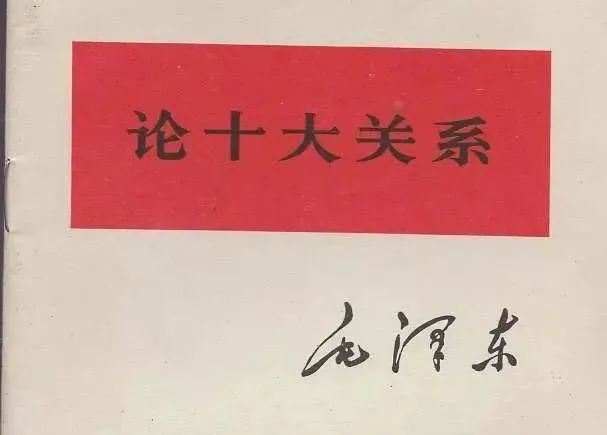
\includegraphics[width=0.8\textwidth,keepaspectratio]{chapter_2551632_专题四_社会主义改造理论/unit_6247975_练习题二/question_16841455/title_img_1.png}\end{center}



\textbf{选项:}
\begin{itemize}[leftmargin=*]

  \item A. 《论十大关系》

  \item B. 《新民主主义论》

  \item C. 《关于正确处理人民内部矛盾的问题》

  \item D. 《中国革命和中国共产党》

\end{itemize}

\textbf{正确答案:}
A

\vspace{0.3em}\hrulefill\vspace{0.7em}

\subsubsection*{26. (多选题) \small QID: 16842190 (ParentID: 6247975)}

\textbf{题干:}
1956年起,毛泽东开始探索适合中国特点的社会主义建设道路。与此相联系,毛泽东提出了一系列新思想,主要有: ( )



\textbf{选项:}
\begin{itemize}[leftmargin=*]

  \item A. 强调独立自主地探索适合中国情况的社会主义建设道路

  \item B. 提出以苏联为鉴

  \item C. 提出马克思主义同中国实际的“第二次结合”

  \item D. 强调改革开放

\end{itemize}

\textbf{正确答案:}
A | B | C

\vspace{0.3em}\hrulefill\vspace{0.7em}

\subsubsection*{27. (多选题) \small QID: 16842191 (ParentID: 6247975)}

\textbf{题干:}
关于社会主义现代化建设的积极因素表述正确的是: ( )



\textbf{选项:}
\begin{itemize}[leftmargin=*]

  \item A. 积极因素处于主导、统治地位

  \item B. 是社会主义事业必定胜利的可靠保证

  \item C. 积极因素与消极因素在一定条件下是可以互相转化的

  \item D. 积极因素和消极因素是对立统一的关系

\end{itemize}

\textbf{正确答案:}
A | B | C | D

\vspace{0.3em}\hrulefill\vspace{0.7em}

\subsubsection*{28. (多选题) \small QID: 16842192 (ParentID: 6247975)}

\textbf{题干:}
中国共产党在探索中国建设道路过程中的理论成果有: ( )



\textbf{选项:}
\begin{itemize}[leftmargin=*]

  \item A. 毛泽东《论十大关系》的发表

  \item B. 党在过渡时期总路线的制定

  \item C. 中共“八大”制定的路线

  \item D. 毛泽东《关于正确处理人民内部矛盾的问题》的重要讲话

\end{itemize}

\textbf{正确答案:}
A | C | D

\vspace{0.3em}\hrulefill\vspace{0.7em}

\subsubsection*{29. (多选题) \small QID: 16842193 (ParentID: 6247975)}

\textbf{题干:}
关于《论十大关系》的表述正确的有: ( )



\textbf{选项:}
\begin{itemize}[leftmargin=*]

  \item A. 它是新中国成立以来中央领导集体深入调查研究的成果

  \item B. 它为中共八大的召开作了理论准备

  \item C. 探讨了中央与地方的关系

  \item D. 探讨了沿海工业和内地工业的关系

\end{itemize}

\textbf{正确答案:}
A | B | C | D

\vspace{0.3em}\hrulefill\vspace{0.7em}

\subsubsection*{30. (多选题) \small QID: 16842194 (ParentID: 6247975)}

\textbf{题干:}
1957年2月,毛泽东作了《关于正确处理人民内部矛盾的问题》的讲话,系统论述了社会主义社会矛盾的理论。毛泽东指出: ( )



\textbf{选项:}
\begin{itemize}[leftmargin=*]

  \item A. 矛盾是普遍存在的,社会主义社会同样充满矛盾

  \item B. 社会主义社会的基本矛盾仍然是生产关系和生产力之间、上层建筑和经济基础之间的矛盾,它同旧社会的基本矛盾性质是—样的

  \item C. 社会主义社会的矛盾反映在政治上可以划分为敌我矛盾和人民内部矛盾这两类性质完全不同的矛盾,正确处理人民内部矛盾的问题是社会主义国家政治生活的主题

  \item D. 社会主义社会的矛盾可以通过社会主义制度本身的自我调整和自我完善得到解决

\end{itemize}

\textbf{正确答案:}
A | C | D

\vspace{0.3em}\hrulefill\vspace{0.7em}

\subsubsection*{31. (多选题) \small QID: 16842195 (ParentID: 6247975)}

\textbf{题干:}
社会主义改造的任务完成以后,我国社会的基本矛盾是: ( )



\textbf{选项:}
\begin{itemize}[leftmargin=*]

  \item A. 敌我矛盾

  \item B. 人民内部矛盾

  \item C. 生产力和生产关系的矛盾

  \item D. 经济基础和上层建筑的矛盾

\end{itemize}

\textbf{正确答案:}
C | D

\vspace{0.3em}\hrulefill\vspace{0.7em}

\subsubsection*{32. (多选题) \small QID: 16842196 (ParentID: 6247975)}

\textbf{题干:}
党的八大正确分析了社会主义改造完成后我国社会主要矛盾的变化,指出,社会主义制度在我国已经基本上建立起来了。我们国内的主要矛盾,已经是: ( )



\textbf{选项:}
\begin{itemize}[leftmargin=*]

  \item A. 人民日益增长的物质文化需要同落后的社会生产之间的矛盾

  \item B. 人民对于建立先进的工业国的要求同落后的农业国的现实之间的矛盾

  \item C. 人民对于经济文化迅速发展的需要同当前经济文化不能满足人民需要的状况之间的矛盾

  \item D. 无产阶级和资产阶级的矛盾

\end{itemize}

\textbf{正确答案:}
B | C

\vspace{0.3em}\hrulefill\vspace{0.7em}

\subsubsection*{33. (多选题) \small QID: 16842197 (ParentID: 6247975)}

\textbf{题干:}
关于社会主义两类不同性质的矛盾表述正确的有: ( )



\textbf{选项:}
\begin{itemize}[leftmargin=*]

  \item A. 反映在政治上可以划分为敌我矛盾和人民内部矛盾

  \item B. 人民内部矛盾是非对抗性的矛盾,处理不当就转化为对抗性的矛盾

  \item C. 用专政、说服教育的方法解决敌我矛盾

  \item D. 人民同反抗社会主义主义革命的社会势力和社会集团的矛盾属于人民内部矛盾

\end{itemize}

\textbf{正确答案:}
A | B

\vspace{0.3em}\hrulefill\vspace{0.7em}

\subsubsection*{34. (多选题) \small QID: 16842198 (ParentID: 6247975)}

\textbf{题干:}
毛泽东在《论十大关系》中指出,正确处理人民内部矛盾的方针、原则包括: ( )



\textbf{选项:}
\begin{itemize}[leftmargin=*]

  \item A. “团结—批评—团结”

  \item B. 实行统筹兼顾、适当安排的方针

  \item C. “百花齐放、百家争鸣”

  \item D. “长期共存,互相监督”

\end{itemize}

\textbf{正确答案:}
A | B | C | D

\vspace{0.3em}\hrulefill\vspace{0.7em}

\subsubsection*{35. (多选题) \small QID: 16842199 (ParentID: 6247975)}

\textbf{题干:}
毛泽东提出的社会主义现代化建设“两步走”的发展战略是: ( )



\textbf{选项:}
\begin{itemize}[leftmargin=*]

  \item A. 第一步建成一个独立的比较完整的工业体系和国民经济体系

  \item B. 第一步使中国逐步由农业国转变为工业国

  \item C. 第二步全面实现工业、农业、国防和科学技术现代化,使中国走在世界前列

  \item D. 第二步到本世纪末全面实现现代化,人民生活达到小康水平

\end{itemize}

\textbf{正确答案:}
A | C

\vspace{0.3em}\hrulefill\vspace{0.7em}

\subsection*{练习题三}

\subsubsection*{36. (多选题) \small QID: 16842200 (ParentID: 6247978)}

\textbf{题干:}
我党在社会主义建设道路初步探索中提出的重要思想理论观点包括: ( )



\textbf{选项:}
\begin{itemize}[leftmargin=*]

  \item A. 社会主义发展两阶段理论

  \item B. 社会主义现代化建设“两步走”发展战略

  \item C. 资本主义经济是社会主义经济的有益补充

  \item D. 要建立适合我国情况和人民需要的社会主义的市场

\end{itemize}

\textbf{正确答案:}
A | B | C | D

\vspace{0.3em}\hrulefill\vspace{0.7em}

\subsubsection*{37. (多选题) \small QID: 16842201 (ParentID: 6247978)}

\textbf{题干:}
20世纪50年代末60,我党关于经济体制的认识表述正确的包括: ( )



\textbf{选项:}
\begin{itemize}[leftmargin=*]

  \item A. 发展商品生产,利用价值规律

  \item B. 社会主义经济应既有计划又有多样性和灵活性

  \item C. 初步建立社会主义市场经济体制

  \item D. 建立适合我国情况和人民需要的社会主义的市场

\end{itemize}

\textbf{正确答案:}
A | B | D

\vspace{0.3em}\hrulefill\vspace{0.7em}

\subsubsection*{38. (多选题) \small QID: 16842202 (ParentID: 6247978)}

\textbf{题干:}
中共八大指出进一步加强社会主义民主政治建设必须做到: ( )



\textbf{选项:}
\begin{itemize}[leftmargin=*]

  \item A. 加强党对国家机关的领导和监督

  \item B. 系统地制定比较完备的法律,健全发展

  \item C. 团结一切可以团结的力量,把当前的注意力转到社会主义建设上来

  \item D. 加强民主集中制

\end{itemize}

\textbf{正确答案:}
A | B | D

\vspace{0.3em}\hrulefill\vspace{0.7em}

\subsubsection*{39. (多选题) \small QID: 16842203 (ParentID: 6247978)}

\textbf{题干:}
毛泽东关于社会主义发展阶段的观点表述正确的是: ( )



\textbf{选项:}
\begin{itemize}[leftmargin=*]

  \item A. 第一个阶段是不发达的社会主义

  \item B. 第二个阶段是比较发达的社会主义

  \item C. 不发达的社会主义比比较发达的社会主义需要更长的时间

  \item D. 第二个阶段是相对发达的社会主义

\end{itemize}

\textbf{正确答案:}
A | B

\vspace{0.3em}\hrulefill\vspace{0.7em}

\subsubsection*{40. (多选题) \small QID: 16842204 (ParentID: 6247978)}

\textbf{题干:}
党领导人民探索社会主义建设道路,历经艰辛和曲折,在理论和实践上取得了一系列重要成果。这些成果具有重要意义: ( )



\textbf{选项:}
\begin{itemize}[leftmargin=*]

  \item A. 巩固和发展了我国的社会主义制度

  \item B. 为开创中国特色社会主义提供了宝贵经验、理论准备、物质基础

  \item C. 丰富了科学社会主义的理论和实践

  \item D. 为其他国家的社会主义建设提供了经验和借鉴

\end{itemize}

\textbf{正确答案:}
A | B | C | D

\vspace{0.3em}\hrulefill\vspace{0.7em}

\subsection*{练习题四}

\subsubsection*{41. (单选题) \small QID: 16840044 (ParentID: 6247982)}

\textbf{题干:}
19世纪60年代初,周恩来将我们党提出的一系列和平解决台湾问题的思想、政策和主张归纳为()



\textbf{选项:}
\begin{itemize}[leftmargin=*]

  \item A. “和为贵”

  \item B. “爱国一家”

  \item C. “爱国不分先后”

  \item D. “一纲四目”

\end{itemize}

\textbf{正确答案:}
D

\vspace{0.3em}\hrulefill\vspace{0.7em}

\subsubsection*{42. (单选题) \small QID: 16840043 (ParentID: 6247982)}

\textbf{题干:}
下列理论成果,不属于社会主义建设道路初步探索时期提出的是()



\textbf{选项:}
\begin{itemize}[leftmargin=*]

  \item A. “四个现代化”战略目标

  \item B. 社会主义初级阶段

  \item C. 祖国统一和外交工作

  \item D. 走中国工业化道路

\end{itemize}

\textbf{正确答案:}
B

\vspace{0.3em}\hrulefill\vspace{0.7em}

\subsubsection*{43. (单选题) \small QID: 16840042 (ParentID: 6247982)}

\textbf{题干:}
社会主义建设道路初步探索时期,提出发展商品生产、利用价值规律的思想的是()



\textbf{选项:}
\begin{itemize}[leftmargin=*]

  \item A. 毛泽东

  \item B. 刘少奇

  \item C. 陈云

  \item D. 邓小平

\end{itemize}

\textbf{正确答案:}
A

\vspace{0.3em}\hrulefill\vspace{0.7em}

\subsubsection*{44. (单选题) \small QID: 16840041 (ParentID: 6247982)}

\textbf{题干:}
社会主义建设道路初步探索时期,提出要建立“适合于我国情况和人民需要的社会主义的市场”的思想的是()



\textbf{选项:}
\begin{itemize}[leftmargin=*]

  \item A. 毛泽东

  \item B. 刘少奇

  \item C. 陈云

  \item D. 邓小平

\end{itemize}

\textbf{正确答案:}
C

\vspace{0.3em}\hrulefill\vspace{0.7em}

\subsubsection*{45. (单选题) \small QID: 16840040 (ParentID: 6247982)}

\textbf{题干:}
在《关于正确处理人民内部矛盾的问题》中,毛泽东明确提出了走中国工业化道路的问题,主要是指()



\textbf{选项:}
\begin{itemize}[leftmargin=*]

  \item A. “以苏为师”还是“以苏为鉴”的问题

  \item B. 重工业和轻工业、农业的发展关系问题

  \item C. 正确处理敌我矛盾和人民内部矛盾

  \item D. 在自力更生的基础上积极争取外援

\end{itemize}

\textbf{正确答案:}
B

\vspace{0.3em}\hrulefill\vspace{0.7em}

\subsubsection*{46. (单选题) \small QID: 16840039 (ParentID: 6247982)}

\textbf{题干:}
为我国实现工业化提供了根本的政治前提是()



\textbf{选项:}
\begin{itemize}[leftmargin=*]

  \item A. 中国共产党的成立

  \item B. 新中国的成立

  \item C. 改革开放

  \item D. 中国特色社会主义道路

\end{itemize}

\textbf{正确答案:}
B

\vspace{0.3em}\hrulefill\vspace{0.7em}

\subsubsection*{47. (单选题) \small QID: 16840038 (ParentID: 6247982)}

\textbf{题干:}
社会主义建设道路初步探索时期,毛泽东强调,()是社会主义国家政治生活的主题。



\textbf{选项:}
\begin{itemize}[leftmargin=*]

  \item A. 调动一切积极因素为社会主义事业服务

  \item B. 关于正确处理人民内部矛盾的问题

  \item C. 走中国工业化道路

  \item D. 实现祖国完全统一

\end{itemize}

\textbf{正确答案:}
B

\vspace{0.3em}\hrulefill\vspace{0.7em}

\subsubsection*{48. (单选题) \small QID: 16840037 (ParentID: 6247982)}

\textbf{题干:}
社会主义建设道路初步探索时期,针对人民内部矛盾在具体实践中的不同情况,毛泽东提出了一系列具体方针、原则。对于政治思想领域的人民内部矛盾()



\textbf{选项:}
\begin{itemize}[leftmargin=*]

  \item A. 实行“百花齐放、百家争鸣”的方针,通过自由讨论和科学实践、艺术实践去解决

  \item B. 实行统筹兼顾、适当安排的方针,兼顾国家、集体和个人三方面的利益

  \item C. 要坚持民主集中制原则,努力克服政府机关的官僚主义,也要加强对群众的思想教育

  \item D. 实行“团结—批评一团结”的方针,坚持说服教育、讨论的方法

\end{itemize}

\textbf{正确答案:}
D

\vspace{0.3em}\hrulefill\vspace{0.7em}

\subsubsection*{49. (单选题) \small QID: 16840036 (ParentID: 6247982)}

\textbf{题干:}
社会主义建设道路初步探索时期,解决人民内部矛盾的总方针是()



\textbf{选项:}
\begin{itemize}[leftmargin=*]

  \item A. 采用专政和民主两种方法

  \item B. “团结—批评—团结”

  \item C. 用民主的方法

  \item D. 用专政的方法

\end{itemize}

\textbf{正确答案:}
C

\vspace{0.3em}\hrulefill\vspace{0.7em}

\subsubsection*{50. (单选题) \small QID: 16840035 (ParentID: 6247982)}

\textbf{题干:}
党的八大正确分析了社会主义改造完成后我国社会主要矛盾的变化,指出,社会主义制度在我国已经基本上建立起来了。我们国内的主要矛盾,已经是()



\textbf{选项:}
\begin{itemize}[leftmargin=*]

  \item A. 人民日益增长的物质文化需要同落后的社会生产之间的矛盾

  \item B. 人民对于建立先进的农业国的要求同落后的工业国的现实之间的矛盾

  \item C. 人民对于经济文化迅速发展的需要同当前经济文化不能满足人民需要的状况之间的矛盾

  \item D. 无产阶级和资产阶级的矛盾

\end{itemize}

\textbf{正确答案:}
C

\vspace{0.3em}\hrulefill\vspace{0.7em}

\subsubsection*{51. (单选题) \small QID: 16840034 (ParentID: 6247982)}

\textbf{题干:}
毛泽东在《关于正确处理人民内部矛盾的问题》的报告中指出,社会主义社会的基本矛盾是()



\textbf{选项:}
\begin{itemize}[leftmargin=*]

  \item A. 人民内部的非对抗性的矛盾

  \item B. 生产关系和生产力之间、上层建筑和经济基础之间的矛盾

  \item C. 无产阶级和资产阶级之间、社会主义和资本主义之间的矛盾

  \item D. 人民日益增长的物质文化需要同落后的社会生产之间的矛盾

\end{itemize}

\textbf{正确答案:}
B

\vspace{0.3em}\hrulefill\vspace{0.7em}

\subsubsection*{52. (单选题) \small QID: 16840033 (ParentID: 6247982)}

\textbf{题干:}
毛泽东系统论述社会主义社会矛盾理论的著作是:



\textbf{选项:}
\begin{itemize}[leftmargin=*]

  \item A. 《关于正确处理人民内部矛盾的问题》

  \item B. 《新民主主义论》

  \item C. 《论十大关系》

  \item D. 《中国社会各阶级的分析》

\end{itemize}

\textbf{正确答案:}
A

\vspace{0.3em}\hrulefill\vspace{0.7em}

\subsubsection*{53. (单选题) \small QID: 16840032 (ParentID: 6247982)}

\textbf{题干:}
《论十大关系》的前五条主要讨论经济问题,其中前三条讲重工业和轻工业、农业的关系,沿海工业和内地工业的关系,经济建设和国防建设的关系。这实际上明确提出了()



\textbf{选项:}
\begin{itemize}[leftmargin=*]

  \item A. 中国的工业化道路问题

  \item B. 中国的经济建设问题

  \item C. 中国的工业发展问题

  \item D. 工业发展的平衡问题

\end{itemize}

\textbf{正确答案:}
A

\vspace{0.3em}\hrulefill\vspace{0.7em}

\subsubsection*{54. (单选题) \small QID: 16840031 (ParentID: 6247982)}

\textbf{题干:}
《论十大关系》第一条主要讨论()



\textbf{选项:}
\begin{itemize}[leftmargin=*]

  \item A. 重工业和轻工业的关系

  \item B. 重工业和轻工业、农业的关系

  \item C. 沿海工业和内地工业的关系

  \item D. 经济建设和国防建设的关系

\end{itemize}

\textbf{正确答案:}
B

\vspace{0.3em}\hrulefill\vspace{0.7em}

\subsubsection*{55. (单选题) \small QID: 16840029 (ParentID: 6247982)}

\textbf{题干:}
《论十大关系》的报告围绕的基本方针是()



\textbf{选项:}
\begin{itemize}[leftmargin=*]

  \item A. 独立自主

  \item B. 自力更生为主,争取外援为辅

  \item C. 调动一切积极因素,为社会主义事业服务

  \item D. 走中国特色社会主义道路

\end{itemize}

\textbf{正确答案:}
C

\vspace{0.3em}\hrulefill\vspace{0.7em}

\subsubsection*{56. (单选题) \small QID: 16840028 (ParentID: 6247982)}

\textbf{题干:}
毛泽东明确提出以苏为鉴,独立自主地探索适合中国情况的社会主义建设道路的著作是()



\textbf{选项:}
\begin{itemize}[leftmargin=*]

  \item A. 《论十大关系》

  \item B. 《新民主主义论》

  \item C. 《关于正确处理人民内部矛盾的问题》

  \item D. 《中国革命和中国共产党》

\end{itemize}

\textbf{正确答案:}
A

\vspace{0.3em}\hrulefill\vspace{0.7em}

\subsubsection*{57. (多选题) \small QID: 16840080 (ParentID: 6247982)}

\textbf{题干:}
根据形势的发展,毛泽东提出两个“中间地带”战略思想,下列说法正确的是()



\textbf{选项:}
\begin{itemize}[leftmargin=*]

  \item A. 亚洲、非洲、拉丁美洲是第一个中间地带

  \item B. 欧洲、北美加拿大、大洋洲加上日本是第二个中间地带

  \item C. 争取“中间地带”,发展同亚非拉国家的关系,成为当时中国对外政策的一个重要组成部分。

  \item D. 两个“中间地带”都反对美国的控制,在东欧各国则发生反对苏联控制的问题。

\end{itemize}

\textbf{正确答案:}
A | B | C | D

\vspace{0.3em}\hrulefill\vspace{0.7em}

\subsubsection*{58. (多选题) \small QID: 16840069 (ParentID: 6247982)}

\textbf{题干:}
20世纪70年代前期,毛泽东针对当时国际形势的变化逐渐形成了关于“三个世界划分”的战略思想。他认为()



\textbf{选项:}
\begin{itemize}[leftmargin=*]

  \item A. 以美国为首的西方发达资本主义国家属于第一世界

  \item B. 苏美两个超级大国属于第一世界

  \item C. 亚洲、非洲、拉丁美洲的广大发展中国家属于第三世界

  \item D. 我们的主要任务是反对超级大国的霸权主义和战争威胁

\end{itemize}

\textbf{正确答案:}
B | C | D

\vspace{0.3em}\hrulefill\vspace{0.7em}

\subsubsection*{59. (多选题) \small QID: 16840060 (ParentID: 6247982)}

\textbf{题干:}
下列关于“三线建设”,说法正确的有()



\textbf{选项:}
\begin{itemize}[leftmargin=*]

  \item A. “三线建设”是20世纪60-70年代我国以加强国防为中心的战略大后方建设。

  \item B. 表明我国经济建设的战略重点发生了向备战倾斜的重大转变。

  \item C. 总目标是采取多快好省的方法,在纵深地区建立起一个工农业结合的、为国防和农业服务的比较完整的战略后方基地。

  \item D. 目的是为了实现祖国完全统一。

\end{itemize}

\textbf{正确答案:}
A | B | C

\vspace{0.3em}\hrulefill\vspace{0.7em}

\subsubsection*{60. (多选题) \small QID: 16840059 (ParentID: 6247982)}

\textbf{题干:}
毛泽东关于社会主义发展阶段的思想,正确的有()



\textbf{选项:}
\begin{itemize}[leftmargin=*]

  \item A. 可能分为两个阶段,第一个阶段是社会主义初级阶段,第二个阶段是社会主义高级阶段

  \item B. 可能分为两个阶段,第一个阶段是不发达的社会主义,第二个阶段是比较发达的社会主义

  \item C. 后一阶段可能比前一阶段需要更长的时间

  \item D. 经过后一阶段,到了物质产品、精神财富都极为丰富和人们的共产主义觉悟极大提高的时候,就可以进入共产主义社会了。

\end{itemize}

\textbf{正确答案:}
B | C | D

\vspace{0.3em}\hrulefill\vspace{0.7em}

\subsection*{练习题五}

\subsubsection*{61. (多选题) \small QID: 16840051 (ParentID: 6247984)}

\textbf{题干:}
我国社会主义改造完成后,根据毛泽东社会主义矛盾学说,属于人民内部矛盾的是()



\textbf{选项:}
\begin{itemize}[leftmargin=*]

  \item A. 工人、农民同知识分子之间的矛盾

  \item B. 工人阶级和其他劳动者同民族资产阶级之间的矛盾

  \item C. 人民同反抗社会主义主义革命的社会势力和社会集团的矛盾

  \item D. 工农两个阶级之间的矛盾

\end{itemize}

\textbf{正确答案:}
A | B | D

\vspace{0.3em}\hrulefill\vspace{0.7em}

\subsubsection*{62. (多选题) \small QID: 16840050 (ParentID: 6247984)}

\textbf{题干:}
社会主义建设道路初步探索时期,毛泽东关于社会主义两类不同性质的矛盾表述,正确的有()



\textbf{选项:}
\begin{itemize}[leftmargin=*]

  \item A. 可以划分为敌我矛盾和人民内部矛盾

  \item B. 人民内部矛盾是非对抗性的矛盾,如果处理不当,也可能发生对抗

  \item C. 用专政的方法解决敌我矛盾

  \item D. 工人阶级和其他劳动者同民族资产阶级之间的矛盾属于敌我矛盾

\end{itemize}

\textbf{正确答案:}
A | B | C

\vspace{0.3em}\hrulefill\vspace{0.7em}

\subsubsection*{63. (多选题) \small QID: 16840049 (ParentID: 6247984)}

\textbf{题干:}
社会主义改造的任务完成以后,我国社会的基本矛盾是:



\textbf{选项:}
\begin{itemize}[leftmargin=*]

  \item A. 敌我矛盾

  \item B. 人民内部矛盾

  \item C. 生产力和生产关系的矛盾

  \item D. 经济基础和上层建筑的矛盾

\end{itemize}

\textbf{正确答案:}
C | D

\vspace{0.3em}\hrulefill\vspace{0.7em}

\subsubsection*{64. (多选题) \small QID: 16840048 (ParentID: 6247984)}

\textbf{题干:}
1957年2月,毛泽东作了《关于正确处理人民内部矛盾的问题》的讲话,系统论述了社会主义社会矛盾的理论。毛泽东指出()



\textbf{选项:}
\begin{itemize}[leftmargin=*]

  \item A. 矛盾是普遍存在的,社会主义社会同样充满矛盾

  \item B. 社会主义社会的基本矛盾仍然是生产关系和生产力之间、上层建筑和经济基础之间的矛盾,它同旧社会的基本矛盾性质是一样的

  \item C. 社会主义社会的矛盾反映在政治上可以划分为敌我矛盾和人民内部矛盾这两类性质完全不同的矛盾,正确处理人民内部矛盾的问题是社会主义国家政治生活的主题

  \item D. 社会主义社会的矛盾可以通过社会主义制度本身的自我调整和自我完善得到解决

\end{itemize}

\textbf{正确答案:}
A | C | D

\vspace{0.3em}\hrulefill\vspace{0.7em}

\subsubsection*{65. (多选题) \small QID: 16840047 (ParentID: 6247984)}

\textbf{题干:}
调动一切积极因素为社会主义事业服务,必须()



\textbf{选项:}
\begin{itemize}[leftmargin=*]

  \item A. 坚持中国共产党的领导

  \item B. 发展社会主义民主政治

  \item C. 确保积极因素和消极因素不发生转化

  \item D. 完全消灭社会矛盾

\end{itemize}

\textbf{正确答案:}
A | B

\vspace{0.3em}\hrulefill\vspace{0.7em}

\subsubsection*{66. (多选题) \small QID: 16840046 (ParentID: 6247984)}

\textbf{题干:}
党在社会主义建设道路的初步探索中取得的重要理论成果包括()



\textbf{选项:}
\begin{itemize}[leftmargin=*]

  \item A. 调动一切积极因素为社会主义事业服务

  \item B. 正确认识和处理社会主义社会矛盾

  \item C. 走中国工业化道路

  \item D. 走中国特色社会主义道路

\end{itemize}

\textbf{正确答案:}
A | B | C

\vspace{0.3em}\hrulefill\vspace{0.7em}

\subsubsection*{67. (判断题) \small QID: 16840082 (ParentID: 6247984)}

\textbf{题干:}
社会主义建设道路初步探索时期,毛泽东提出了发展商品生产、利用价值规律的思想,认为商品生产在社会主义条件下,还是一个不可缺少的、有利的工具,要有计划地大大地发展社会主义的商品生产。



\textbf{正确答案:}
true

\vspace{0.3em}\hrulefill\vspace{0.7em}

\subsection*{练习题二}

\subsubsection*{68. (单选题) \small QID: 16841355 (ParentID: 6273520)}

\textbf{题干:}
中国共产党提出由新民主主义社会和平过渡到社会主义社会的最初设想是 ( )



\textbf{选项:}
\begin{itemize}[leftmargin=*]

  \item A. 民主革命时期

  \item B. 中华人民共和国成立后

  \item C. 社会主义改造完成后

  \item D. “文化大革命”时期

\end{itemize}

\textbf{正确答案:}
A

\vspace{0.3em}\hrulefill\vspace{0.7em}

\subsubsection*{69. (单选题) \small QID: 16841356 (ParentID: 6273520)}

\textbf{题干:}
1952年底,随着土地改革的基本完成,我国社会的主要矛盾已转变成 ( )



\textbf{选项:}
\begin{itemize}[leftmargin=*]

  \item A. 人民大众同帝国主义、封建主义及其走狗国民党反动派残余的矛盾

  \item B. 帝国主义和中华民族的矛盾、封建主义和人民大众的矛盾

  \item C. 工人阶级同资产阶级的矛盾、社会主义道路同资本主义道路的矛盾

  \item D. 人民日益增长的物质文化需要同落后的社会生产之间的矛盾

\end{itemize}

\textbf{正确答案:}
C

\vspace{0.3em}\hrulefill\vspace{0.7em}

\subsubsection*{70. (单选题) \small QID: 16841357 (ParentID: 6273520)}

\textbf{题干:}
新民主主义社会中,处于领导地位的经济成分是 ( )



\textbf{选项:}
\begin{itemize}[leftmargin=*]

  \item A. 个体经济

  \item B. 私人和国家资本主义经济

  \item C. 国营经济

  \item D. 合作社经济

\end{itemize}

\textbf{正确答案:}
C

\vspace{0.3em}\hrulefill\vspace{0.7em}

\subsubsection*{71. (单选题) \small QID: 16841358 (ParentID: 6273520)}

\textbf{题干:}
建国初期,我国社会主义国营经济建立的最主要途径和手段是 ( )



\textbf{选项:}
\begin{itemize}[leftmargin=*]

  \item A. 没收帝国主义在华企业

  \item B. 没收官僚资本

  \item C. 没收民族资本

  \item D. 没收地主阶级的土地和财产

\end{itemize}

\textbf{正确答案:}
B

\vspace{0.3em}\hrulefill\vspace{0.7em}

\subsubsection*{72. (单选题) \small QID: 16841359 (ParentID: 6273520)}

\textbf{题干:}
从中华人民共和国成立到社会主义改造基本完成,是我国从新民主主义到社会主义的过渡时期,这一时期,个体经济向社会主义集体经济过渡的形式是 ( )



\textbf{选项:}
\begin{itemize}[leftmargin=*]

  \item A. 国营经济

  \item B. 私人资本主义经济

  \item C. 国家资本主义经济

  \item D. 合作社经济

\end{itemize}

\textbf{正确答案:}
D

\vspace{0.3em}\hrulefill\vspace{0.7em}

\subsubsection*{73. (单选题) \small QID: 16841360 (ParentID: 6273520)}

\textbf{题干:}
毛泽东关于农业社会主义改造理论来源是 ( )



\textbf{选项:}
\begin{itemize}[leftmargin=*]

  \item A. 马克思的合作化理论

  \item B. 恩格斯的合作化理论

  \item C. 列宁的合作化理论

  \item D. 斯大林的合作化理论

\end{itemize}

\textbf{正确答案:}
C

\vspace{0.3em}\hrulefill\vspace{0.7em}

\subsubsection*{74. (单选题) \small QID: 16841361 (ParentID: 6273520)}

\textbf{题干:}
标志着资本主义工商业的社会主义改造已经基本完成是实现了 ( )



\textbf{选项:}
\begin{itemize}[leftmargin=*]

  \item A. 手工业合作社的建立

  \item B. 农业合作化

  \item C. 全行业公私合营

  \item D. 生产责任制

\end{itemize}

\textbf{正确答案:}
C

\vspace{0.3em}\hrulefill\vspace{0.7em}

\subsubsection*{75. (单选题) \small QID: 16841362 (ParentID: 6273520)}

\textbf{题干:}
过渡时期总路线的主体是 ( )



\textbf{选项:}
\begin{itemize}[leftmargin=*]

  \item A. 国家的社会主义工业化

  \item B. 私营经济的国有化

  \item C. 个体农业的集体化

  \item D. 对个体农业、手工业和资本主义工商业的改造

\end{itemize}

\textbf{正确答案:}
A

\vspace{0.3em}\hrulefill\vspace{0.7em}

\subsubsection*{76. (单选题) \small QID: 16841363 (ParentID: 6273520)}

\textbf{题干:}
关于社会主义过渡时期总路线错误的说法是 ( )



\textbf{选项:}
\begin{itemize}[leftmargin=*]

  \item A. 实现社会主义工业化,农业、手工业和资本主义工商业的社会主义改造

  \item B. 过渡时期结束的标志是社会主义改造结束

  \item C. 以单一的社会主义公有制和计划经济体制为目标

  \item D. 以中国特色社会主义为目标

\end{itemize}

\textbf{正确答案:}
D

\vspace{0.3em}\hrulefill\vspace{0.7em}

\subsubsection*{77. (单选题) \small QID: 16841364 (ParentID: 6273520)}

\textbf{题干:}
党在过渡时期总路线的实质是 ( )



\textbf{选项:}
\begin{itemize}[leftmargin=*]

  \item A. 改变生产资料的私有制

  \item B. 发展生产力

  \item C. 消灭剥削阶级

  \item D. 改造个体农民和手工业者

\end{itemize}

\textbf{正确答案:}
A

\vspace{0.3em}\hrulefill\vspace{0.7em}

\subsubsection*{78. (单选题) \small QID: 16841365 (ParentID: 6273520)}

\textbf{题干:}
中国社会主义改造和社会主义建设道路中一个十分突出的特殊问题是 ( )



\textbf{选项:}
\begin{itemize}[leftmargin=*]

  \item A. 一个落后的农业国的工业化问题

  \item B. 农业的社会主义改造问题

  \item C. 农业的机械化问题

  \item D. 民族资本主义工商业的社会主义改造问题

\end{itemize}

\textbf{正确答案:}
A

\vspace{0.3em}\hrulefill\vspace{0.7em}

\subsubsection*{79. (单选题) \small QID: 16841366 (ParentID: 6273520)}

\textbf{题干:}
制定我国第一个五年计划的依据是 ( )



\textbf{选项:}
\begin{itemize}[leftmargin=*]

  \item A. 国民经济的恢复和发展

  \item B. 土地改革的完成

  \item C. 实现国家工业化

  \item D. 过渡时期的总路线

\end{itemize}

\textbf{正确答案:}
D

\vspace{0.3em}\hrulefill\vspace{0.7em}

\subsubsection*{80. (单选题) \small QID: 16841367 (ParentID: 6273520)}

\textbf{题干:}
中国共产党对个体农业和手工业实行社会主义改造的方针是 ( )



\textbf{选项:}
\begin{itemize}[leftmargin=*]

  \item A. 趁热打铁,积极领导

  \item B. 自愿互利,国家帮助

  \item C. 积极领导,稳步前进

  \item D. 国家帮助,典型示范

\end{itemize}

\textbf{正确答案:}
C

\vspace{0.3em}\hrulefill\vspace{0.7em}

\subsubsection*{81. (单选题) \small QID: 16841368 (ParentID: 6273520)}

\textbf{题干:}
我国在手工业的社会主义改造过程中所办的手工业生产合作社属于 ( )



\textbf{选项:}
\begin{itemize}[leftmargin=*]

  \item A. 社会主义性质

  \item B. 半社会主义性质

  \item C. 社会主义萌芽性质

  \item D. 非社会主义性质

\end{itemize}

\textbf{正确答案:}
A

\vspace{0.3em}\hrulefill\vspace{0.7em}

\subsubsection*{82. (单选题) \small QID: 16841369 (ParentID: 6273520)}

\textbf{题干:}
中国共产党对资本主义工商业进行社会主义改造的主要方式是 ( )



\textbf{选项:}
\begin{itemize}[leftmargin=*]

  \item A. 和平赎买

  \item B. 统购统销

  \item C. 公私合营

  \item D. 合作化

\end{itemize}

\textbf{正确答案:}
A

\vspace{0.3em}\hrulefill\vspace{0.7em}

\subsubsection*{83. (单选题) \small QID: 16841370 (ParentID: 6273520)}

\textbf{题干:}
我国对资本主义工商业改造创造了国家资本主义的各种形式,其高级形式是 ( )



\textbf{选项:}
\begin{itemize}[leftmargin=*]

  \item A. 统购包销

  \item B. 委托加工,计划订货

  \item C. 经销、代销

  \item D. 公私合营

\end{itemize}

\textbf{正确答案:}
D

\vspace{0.3em}\hrulefill\vspace{0.7em}

\subsubsection*{84. (单选题) \small QID: 16841371 (ParentID: 6273520)}

\textbf{题干:}
我国在对资产阶级工商业实行社会主义改造的过程中,国家向私营企业投资入股,企业生产资料由国家和资本家共同所有,利润分配仍然实行“四马分肥”,国家向企业派出公方代表,与工人、资本家共同管理和改造企业,公方代表居领导地位。这时的企业性质 ( )



\textbf{选项:}
\begin{itemize}[leftmargin=*]

  \item A. 仍然属于私营企业

  \item B. 属于半社会主义性质

  \item C. 具有了社会主义因素

  \item D. 基本上属于社会主义国营性质

\end{itemize}

\textbf{正确答案:}
B

\vspace{0.3em}\hrulefill\vspace{0.7em}

\subsubsection*{85. (单选题) \small QID: 16841372 (ParentID: 6273520)}

\textbf{题干:}
在我国的过渡性质时期,民族资产阶级与工人阶级的矛盾性质是 ( )



\textbf{选项:}
\begin{itemize}[leftmargin=*]

  \item A. 对抗性的

  \item B. 非对抗性的

  \item C. 既有对抗性一面又有非对抗性的一面

  \item D. 没有矛盾

\end{itemize}

\textbf{正确答案:}
C

\vspace{0.3em}\hrulefill\vspace{0.7em}

\subsubsection*{86. (单选题) \small QID: 16841373 (ParentID: 6273520)}

\textbf{题干:}
我国进入社会主义初级阶段的起点及剥削阶级和剥削制度被消灭的标志是 ( )



\textbf{选项:}
\begin{itemize}[leftmargin=*]

  \item A. 社会主义改造的完成

  \item B. 国民经济恢复任务的完成

  \item C. 中华人民共和国的成立

  \item D. 中共十三大的召开

\end{itemize}

\textbf{正确答案:}
A

\vspace{0.3em}\hrulefill\vspace{0.7em}

\subsubsection*{87. (单选题) \small QID: 16841374 (ParentID: 6273520)}

\textbf{题干:}
1956年,社会主义改造基本完成以后,我国社会的主要矛盾是 ( )



\textbf{选项:}
\begin{itemize}[leftmargin=*]

  \item A. 工人阶级和资产阶级的矛盾

  \item B. 社会主义道路和资本主义道路之间的矛盾

  \item C. 人民日益增长的物质文化生活需要同落后的社会生产之间的矛盾

  \item D. 坚持思想基本原则和资产阶级自由化之间的矛盾

\end{itemize}

\textbf{正确答案:}
C

\vspace{0.3em}\hrulefill\vspace{0.7em}

\subsection*{练习题三}

\subsubsection*{88. (多选题) \small QID: 16841376 (ParentID: 6273521)}

\textbf{题干:}
关于中国新民主主义社会,下列说法正确的是 ( )



\textbf{选项:}
\begin{itemize}[leftmargin=*]

  \item A. 就全国范围来讲,它是指从1949年中华人民共和国的成立到1956年社会主义改造的基本完成

  \item B. 它是一个过渡性质的社会,类似于马克思列宁所说的过渡时期

  \item C. 它从属于社会主义范畴

  \item D. 它与社会主义初级阶段本质上是相同的

\end{itemize}

\textbf{正确答案:}
A | B | C

\vspace{0.3em}\hrulefill\vspace{0.7em}

\subsubsection*{89. (多选题) \small QID: 16841377 (ParentID: 6273521)}

\textbf{题干:}
从中华人民共和国成立到社会主义改造基本完成,是我国从新民主主义到社会主义的过渡时期。这一时期中国社会的阶级构成主要包括 ( )



\textbf{选项:}
\begin{itemize}[leftmargin=*]

  \item A. 工人阶级

  \item B. 农民阶级

  \item C. 民族资产阶级

  \item D. 城市小资产阶级

\end{itemize}

\textbf{正确答案:}
A | B | C | D

\vspace{0.3em}\hrulefill\vspace{0.7em}

\subsubsection*{90. (多选题) \small QID: 16841378 (ParentID: 6273521)}

\textbf{题干:}
在新民主主义社会中,主要的经济成分有哪几种 ( )



\textbf{选项:}
\begin{itemize}[leftmargin=*]

  \item A. 合作社经济

  \item B. 个体经济

  \item C. 社会主义经济

  \item D. 资本主义经济

\end{itemize}

\textbf{正确答案:}
B | C | D

\vspace{0.3em}\hrulefill\vspace{0.7em}

\subsubsection*{91. (多选题) \small QID: 16841379 (ParentID: 6273521)}

\textbf{题干:}
1952年党中央在酝酿过渡时期总路线时,毛泽东把实现向社会主义转变的设想,由建国之初的“先搞工业化建设”再一举过渡,改变为“建设和改造同时并举,逐步过渡”,这一改变原因和条件是: ( )



\textbf{选项:}
\begin{itemize}[leftmargin=*]

  \item A. 我国社会主义经济因素的不断增长和对资本主义经济的限制

  \item B. 为了确定我国工业化建设的社会主义方向

  \item C. 我国工业化建设取得了重大成就

  \item D. 民主革命的遗留任务已经完成

\end{itemize}

\textbf{正确答案:}
A | B | D

\vspace{0.3em}\hrulefill\vspace{0.7em}

\subsubsection*{92. (多选题) \small QID: 16841380 (ParentID: 6273521)}

\textbf{题干:}
新中国对个体手工业社会主义改造的主要形式有 ( )



\textbf{选项:}
\begin{itemize}[leftmargin=*]

  \item A. 供销组

  \item B. 供销合作社

  \item C. 生产合作社

  \item D. 公私合营

\end{itemize}

\textbf{正确答案:}
A | B | C

\vspace{0.3em}\hrulefill\vspace{0.7em}

\subsubsection*{93. (多选题) \small QID: 16841381 (ParentID: 6273521)}

\textbf{题干:}
中国共产党根据马克思列宁主义关于农业社会主义改造的思想,从我国的实际出发,开创了一条有中国特点的农业合作化道路,成功实现了对个体农业的社会主义改造,其成功经验主要有 ( )



\textbf{选项:}
\begin{itemize}[leftmargin=*]

  \item A. 在土地改革基础上,不失时机地引导个体农民走互助合作道路

  \item B. 遵循自愿互利、典型示范、国家帮助的原则

  \item C. 实行“三级所有、队为基础”的农村集体经济体制

  \item D. 采取从互助组到初级合作社到高级合作社的逐步过渡形式

\end{itemize}

\textbf{正确答案:}
A | B | D

\vspace{0.3em}\hrulefill\vspace{0.7em}

\subsubsection*{94. (多选题) \small QID: 16841382 (ParentID: 6273521)}

\textbf{题干:}
上世纪50年代,我国在对资本主义工商业进行社会主义改造过程中创造的国家资本主义的具体形式有 ( )



\textbf{选项:}
\begin{itemize}[leftmargin=*]

  \item A. 加工订货

  \item B. 统购包销

  \item C. 经销代销

  \item D. 公私合营

\end{itemize}

\textbf{正确答案:}
A | B | C | D

\vspace{0.3em}\hrulefill\vspace{0.7em}

\subsubsection*{95. (多选题) \small QID: 16841383 (ParentID: 6273521)}

\textbf{题干:}
我国对资本主义工商业进行社会主义改造的经验有 ( )



\textbf{选项:}
\begin{itemize}[leftmargin=*]

  \item A. 严格区别官僚资本和民族资本的界限,实行了和平赎买,和平地实现了和平关系的深刻变革

  \item B. 创造了国家资本主义的多种形式,采取了由低级到高级逐步过渡的形势

  \item C. 把对企业的改造和对资本家的改造结合起来,把资本家改造成自食其力的劳动者

  \item D. 对私人资本主义的赎买政策应始终坚持“四马分肥”

\end{itemize}

\textbf{正确答案:}
A | B | C

\vspace{0.3em}\hrulefill\vspace{0.7em}

\subsubsection*{96. (多选题) \small QID: 16841384 (ParentID: 6273521)}

\textbf{题干:}
新中国对民族资产阶级实行和平赎买的必要性在于 ( )



\textbf{选项:}
\begin{itemize}[leftmargin=*]

  \item A. 民族资产阶级经济实力雄厚,掌握国家经济命脉

  \item B. 民族资产阶级有一定的技术专长和管理经验

  \item C. 民族资产阶级经济构成整个国民经济的基础

  \item D. 中国经济落后,需要利用民族资本主义经济有利于国计民生的一面

\end{itemize}

\textbf{正确答案:}
B | C | D

\vspace{0.3em}\hrulefill\vspace{0.7em}

\subsubsection*{97. (多选题) \small QID: 16841385 (ParentID: 6273521)}

\textbf{题干:}
我国社会主义改造是一场伟大的社会变革,但是在改造过程中也出现了一些偏差,遗留了一些问题,具体表现在 ( )



\textbf{选项:}
\begin{itemize}[leftmargin=*]

  \item A. 所有制结构过于单一,在社会主义公有制已居于绝对统治地位的条件下,没有限度地保留一部分有益于国计民生的个体经济和私营经济

  \item B. 高度集中的计划经济体制也随之扩大到整个社会经济生活

  \item C. 在一定程度上排斥了商品经济和市场经济的正常运行

  \item D. 要求过急,发展过快,工作过粗,改造形式过于简单

\end{itemize}

\textbf{正确答案:}
A | B | C | D

\vspace{0.3em}\hrulefill\vspace{0.7em}

\subsection*{练习题四}

\subsubsection*{98. (单选题) \small QID: 16840004 (ParentID: 6273522)}

\textbf{题干:}
对资本主义工商业的社会主义改造经历的步骤,按顺序为()
\par
①主要实行初级形势的国家资本主义。②实行全行业的公私合营。③主要实行个别企业的公私合营。④用和平赎买的方法改造资本主义工商业。



\textbf{选项:}
\begin{itemize}[leftmargin=*]

  \item A. ④①③②

  \item B. ④③②

  \item C. ①③②

  \item D. ①③④②

\end{itemize}

\textbf{正确答案:}
C

\vspace{0.3em}\hrulefill\vspace{0.7em}

\subsubsection*{99. (单选题) \small QID: 16840003 (ParentID: 6273522)}

\textbf{题干:}
手工业的社会主义改造经历了由小到大、由低级到高级的三个步骤,这三个步骤是()
\par
①办手工业供销小组。②成立互助组。③办手工业供销合作社。④建立初级农业生产合作社。⑤建立手工业生产合作社。⑥发展高级社。



\textbf{选项:}
\begin{itemize}[leftmargin=*]

  \item A. ②④⑥

  \item B. ①③⑤

  \item C. ②③⑤

  \item D. ②③⑥

\end{itemize}

\textbf{正确答案:}
B

\vspace{0.3em}\hrulefill\vspace{0.7em}

\subsubsection*{100. (单选题) \small QID: 16840002 (ParentID: 6273522)}

\textbf{题干:}
对资本主义工商业进行社会主义改造的主要方法是( )



\textbf{选项:}
\begin{itemize}[leftmargin=*]

  \item A. 和平赎买

  \item B. 统购统销

  \item C. 公私合营

  \item D. 合作化

\end{itemize}

\textbf{正确答案:}
A

\vspace{0.3em}\hrulefill\vspace{0.7em}

\subsubsection*{101. (单选题) \small QID: 16840001 (ParentID: 6273522)}

\textbf{题干:}
对个体农业和手工业实行社会主义改造的方针是( )



\textbf{选项:}
\begin{itemize}[leftmargin=*]

  \item A. 趁热打铁,积极领导

  \item B. 自愿互利,国家帮助

  \item C. 积极领导,稳步前进

  \item D. 国家帮助,典型示范

\end{itemize}

\textbf{正确答案:}
C

\vspace{0.3em}\hrulefill\vspace{0.7em}

\subsubsection*{102. (单选题) \small QID: 16840000 (ParentID: 6273522)}

\textbf{题干:}
过渡时期总路线的主体是(  )



\textbf{选项:}
\begin{itemize}[leftmargin=*]

  \item A. 国家的社会主义工业化

  \item B. 私营经济的国有化

  \item C. 个体农业的集体化

  \item D. 对个体农业、手工业和资本主义工商业的改造

\end{itemize}

\textbf{正确答案:}
A

\vspace{0.3em}\hrulefill\vspace{0.7em}

\subsubsection*{103. (单选题) \small QID: 16839999 (ParentID: 6273522)}

\textbf{题干:}
正式批准过渡时期的总路线是在()



\textbf{选项:}
\begin{itemize}[leftmargin=*]

  \item A. 1953年6月,中央政治局会议

  \item B. 1953年6月,党的七届四中全会

  \item C. 1954年2月,中央政治局会议

  \item D. 1954年2月,党的七届四中全会

\end{itemize}

\textbf{正确答案:}
D

\vspace{0.3em}\hrulefill\vspace{0.7em}

\subsubsection*{104. (单选题) \small QID: 16839998 (ParentID: 6273522)}

\textbf{题干:}
随着土地改革的基本完成,我国社会的主要矛盾已转变成(  )



\textbf{选项:}
\begin{itemize}[leftmargin=*]

  \item A. 社会主义道路同资本主义道路的矛盾

  \item B. 帝国主义和中华民族的矛盾、封建主义和人民大众的矛盾

  \item C. 工人阶级同资产阶级的矛盾

  \item D. 人民日益增长的物质文化需要同落后的社会生产之间的矛盾

\end{itemize}

\textbf{正确答案:}
C

\vspace{0.3em}\hrulefill\vspace{0.7em}

\subsubsection*{105. (单选题) \small QID: 16839997 (ParentID: 6273522)}

\textbf{题干:}
从中华人民共和国成立到社会主义改造基本完成,是我国从新民主主义社会到社会主义的过渡时期,这一时期,我国社会的性质是()



\textbf{选项:}
\begin{itemize}[leftmargin=*]

  \item A. 资本主义社会

  \item B. 社会主义社会

  \item C. 民主主义社会

  \item D. 新民主主义社会

\end{itemize}

\textbf{正确答案:}
D

\vspace{0.3em}\hrulefill\vspace{0.7em}

\subsubsection*{106. (多选题) \small QID: 16840011 (ParentID: 6273522)}

\textbf{题干:}
对资本主义工商业实行和平赎买,有利于()



\textbf{选项:}
\begin{itemize}[leftmargin=*]

  \item A. 发挥私营工商业在国计民生方面的积极作用,促进国民经济发展

  \item B. 争取和团结民族资产阶级,有利于团结各民主党派和各界爱国民主人士,巩固和发展统一战线

  \item C. 发挥民族资产阶级中大多数人的知识、才能、技术专长和管理经验

  \item D. 争取和团结那些原来同资产阶级相联系的知识分子为社会主义建设服务。

\end{itemize}

\textbf{正确答案:}
A | B | C | D

\vspace{0.3em}\hrulefill\vspace{0.7em}

\subsubsection*{107. (多选题) \small QID: 16840010 (ParentID: 6273522)}

\textbf{题干:}
在进行社会主义改造、向社会主义过渡的进程中,中国共产党积累了丰富的历史经验,包括()



\textbf{选项:}
\begin{itemize}[leftmargin=*]

  \item A. 坚持社会主义工业化建设与社会主义改造同时并举。

  \item B. 采取积极引导、逐步过渡的方式。

  \item C. 用和平方法进行改造。

  \item D. 采用从低级到高级的国家资本主义的过渡形式。

\end{itemize}

\textbf{正确答案:}
A | B | C

\vspace{0.3em}\hrulefill\vspace{0.7em}

\subsubsection*{108. (多选题) \small QID: 16840009 (ParentID: 6273522)}

\textbf{题干:}
农业社会主义改造大体上经历了()发展阶段



\textbf{选项:}
\begin{itemize}[leftmargin=*]

  \item A. 互助组

  \item B. 初级社

  \item C. 中级社

  \item D. 高级社

\end{itemize}

\textbf{正确答案:}
A | B | D

\vspace{0.3em}\hrulefill\vspace{0.7em}

\subsubsection*{109. (多选题) \small QID: 16840008 (ParentID: 6273522)}

\textbf{题干:}
在新民主主义社会中,主要的经济成分有哪几种(  )



\textbf{选项:}
\begin{itemize}[leftmargin=*]

  \item A. 合作社经济

  \item B. 个体经济

  \item C. 社会主义经济

  \item D. 资本主义经济

\end{itemize}

\textbf{正确答案:}
B | C | D

\vspace{0.3em}\hrulefill\vspace{0.7em}

\subsubsection*{110. (多选题) \small QID: 16840007 (ParentID: 6273522)}

\textbf{题干:}
从中华人民共和国成立到社会主义改造基本完成,是我国从新民主主义到社会主义的过渡时期。这一时期中国社会的阶级构成主要包括(  )



\textbf{选项:}
\begin{itemize}[leftmargin=*]

  \item A. 工人阶级

  \item B. 农民阶级

  \item C. 民族资产阶级

  \item D. 城市小资产阶级

\end{itemize}

\textbf{正确答案:}
A | B | C | D

\vspace{0.3em}\hrulefill\vspace{0.7em}

\subsubsection*{111. (多选题) \small QID: 16840006 (ParentID: 6273522)}

\textbf{题干:}
关于中国新民主主义社会,下列说法正确的是( )



\textbf{选项:}
\begin{itemize}[leftmargin=*]

  \item A. 就时间来讲,它是指从1949年中华人民共和国的成立到1956年社会主义改造的基本完成

  \item B. 它是一个过渡性社会形态

  \item C. 它是一个独立的社会形态

  \item D. 它与社会主义初级阶段本质上是相同的

\end{itemize}

\textbf{正确答案:}
A | B

\vspace{0.3em}\hrulefill\vspace{0.7em}

\subsubsection*{112. (判断题) \small QID: 16840013 (ParentID: 6273522)}

\textbf{题干:}
我国的社会主义改造取得了历史性的胜利,没有出现失误和偏差。



\textbf{正确答案:}
false

\vspace{0.3em}\hrulefill\vspace{0.7em}

\section*{专题五 社会主义建设道路初步探索的理论成果}
\hrulefill

\subsection*{练习题一}

\subsubsection*{1. (单选题) \small QID: 16843213 (ParentID: 6247989)}

\textbf{题干:}
在社会主义建设道路初步探索过程中,关于生产资料所有制调整方面,提出了“三个主体,三个补充”设想的是:



\textbf{选项:}
\begin{itemize}[leftmargin=*]

  \item A. 刘少奇

  \item B. 毛泽东

  \item C. 陈云

  \item D. 邓小平

\end{itemize}

\textbf{正确答案:}
C

\vspace{0.3em}\hrulefill\vspace{0.7em}

\subsubsection*{2. (单选题) \small QID: 16843204 (ParentID: 6247989)}

\textbf{题干:}
成为党探索中国社会主义建设道路良好开端的文章,是毛泽东发表的:



\textbf{选项:}
\begin{itemize}[leftmargin=*]

  \item A. 《论人民民主专政》

  \item B. 《纪念孙中山先生》

  \item C. 《论十大关系》

  \item D. 《关于正确处理人艮内部矛盾的问题》

\end{itemize}

\textbf{正确答案:}
C

\vspace{0.3em}\hrulefill\vspace{0.7em}

\subsubsection*{3. (单选题) \small QID: 16843205 (ParentID: 6247989)}

\textbf{题干:}
《论十大关系》的前五条主要讨论经济问题,其中前三条讲重工业和轻工业、农业的关系,沿海工业和内地工业的关系,经济建设和国防建设的关系。这实际上明确提出了:



\textbf{选项:}
\begin{itemize}[leftmargin=*]

  \item A. 中国的工业化道路问题

  \item B. 中国的工业发展问题

  \item C. 中国的经济建设问题

  \item D. 工业发展的平衡问题

\end{itemize}

\textbf{正确答案:}
A

\vspace{0.3em}\hrulefill\vspace{0.7em}

\subsubsection*{4. (单选题) \small QID: 16843206 (ParentID: 6247989)}

\textbf{题干:}
毛泽东系统论述社会主义社会矛盾理论的著作是:



\textbf{选项:}
\begin{itemize}[leftmargin=*]

  \item A. 《关于正确处理人民内部矛盾的问题》

  \item B. 《新民主主义论》

  \item C. 《论十大关系》

  \item D. 《中国社会各阶级的分析》

\end{itemize}

\textbf{正确答案:}
A

\vspace{0.3em}\hrulefill\vspace{0.7em}

\subsubsection*{5. (单选题) \small QID: 16843207 (ParentID: 6247989)}

\textbf{题干:}
毛泽东在《关于正确处理人民内部矛盾的问题》的报告中指出,社会主义社会的基本矛盾是:



\textbf{选项:}
\begin{itemize}[leftmargin=*]

  \item A. 人民内部的非对抗性的矛盾

  \item B. 生产关系和生产力之间、上层建筑和经济基础之间的矛盾

  \item C. 无产阶级和资产阶级之间、社会主义和资本主义之间的矛盾

  \item D. 人民日益增长的物质文化需要同落后的社会生产之间的矛盾

\end{itemize}

\textbf{正确答案:}
B

\vspace{0.3em}\hrulefill\vspace{0.7em}

\subsubsection*{6. (单选题) \small QID: 16843208 (ParentID: 6247989)}

\textbf{题干:}
毛泽东认为社会主义社会基本矛盾的特点是:



\textbf{选项:}
\begin{itemize}[leftmargin=*]

  \item A. 相适应

  \item B. 相矛盾

  \item C. 又相适应又相矛盾

  \item D. 不相适应又不相矛盾

\end{itemize}

\textbf{正确答案:}
C

\vspace{0.3em}\hrulefill\vspace{0.7em}

\subsubsection*{7. (单选题) \small QID: 16843209 (ParentID: 6247989)}

\textbf{题干:}
下列不属于人民内部矛盾的是:



\textbf{选项:}
\begin{itemize}[leftmargin=*]

  \item A. 工人阶级和农民阶级的矛盾

  \item B. 工人、农民同知识分子之间的矛盾

  \item C. 敌对分子、敌对势力与人民的矛盾

  \item D. 民主同集中的矛盾

\end{itemize}

\textbf{正确答案:}
C

\vspace{0.3em}\hrulefill\vspace{0.7em}

\subsubsection*{8. (单选题) \small QID: 16843210 (ParentID: 6247989)}

\textbf{题干:}
解决敌我矛盾应采用:



\textbf{选项:}
\begin{itemize}[leftmargin=*]

  \item A. 说服的方法

  \item B. 专政的方法

  \item C. 民主的方法

  \item D. 教育的方法

\end{itemize}

\textbf{正确答案:}
B

\vspace{0.3em}\hrulefill\vspace{0.7em}

\subsubsection*{9. (单选题) \small QID: 16843211 (ParentID: 6247989)}

\textbf{题干:}
毛泽东明确提出要走一条有别于苏联的中国工业化道路的著述是:



\textbf{选项:}
\begin{itemize}[leftmargin=*]

  \item A. 《论十大关系》

  \item B. 《关于正确处理人民内部矛盾的问题》

  \item C. 《为争取国家财政经济状况基本好转而斗争》

  \item D. 《在扩大的中央工作会议上的讲话》

\end{itemize}

\textbf{正确答案:}
A

\vspace{0.3em}\hrulefill\vspace{0.7em}

\subsubsection*{10. (单选题) \small QID: 16843212 (ParentID: 6247989)}

\textbf{题干:}
实现我国工业化应坚持的方针不包括:



\textbf{选项:}
\begin{itemize}[leftmargin=*]

  \item A. “两条腿走路”

  \item B. 农业为基础,工业为主导,以农轻重为序

  \item C. 中央工业和地方工业并举

  \item D. 国家、生产单位和生产者个人利益兼顾

\end{itemize}

\textbf{正确答案:}
D

\vspace{0.3em}\hrulefill\vspace{0.7em}

\subsubsection*{11. (多选题) \small QID: 16843215 (ParentID: 6247989)}

\textbf{题干:}
1956年起,毛泽东开始探索适合中国特点的社会主义建设道路。与此相联系,毛泽东提出了一系列新思想,主要有:



\textbf{选项:}
\begin{itemize}[leftmargin=*]

  \item A. 强调独立自主地探索适合中国情况的社会主义建设道路

  \item B. 提出以苏联为鉴

  \item C. 提出马克思主义同中国实际的“第二次结合”

  \item D. 强调改革开放

\end{itemize}

\textbf{正确答案:}
A | B | C

\vspace{0.3em}\hrulefill\vspace{0.7em}

\subsubsection*{12. (多选题) \small QID: 16843216 (ParentID: 6247989)}

\textbf{题干:}
关于《论十大关系》的表述正确的有:



\textbf{选项:}
\begin{itemize}[leftmargin=*]

  \item A. 它是新中国成立以来中央领导集体深入调查研究的成果

  \item B. 它为中共八大的召开作了理论准备

  \item C. 探讨了中央与地方的关系

  \item D. 探讨了沿海工业和内地工业的关系

\end{itemize}

\textbf{正确答案:}
A | B | C | D

\vspace{0.3em}\hrulefill\vspace{0.7em}

\subsubsection*{13. (多选题) \small QID: 16843217 (ParentID: 6247989)}

\textbf{题干:}
社会主义改造的任务完成以后,我国社会的基本矛盾是:



\textbf{选项:}
\begin{itemize}[leftmargin=*]

  \item A. 敌我矛盾

  \item B. 人民内部矛盾

  \item C. 生产力和生产关系的矛盾

  \item D. 经济基础和上层建筑的矛盾

\end{itemize}

\textbf{正确答案:}
C | D

\vspace{0.3em}\hrulefill\vspace{0.7em}

\subsubsection*{14. (多选题) \small QID: 16843218 (ParentID: 6247989)}

\textbf{题干:}
关于社会主义两类不同性质的矛盾表述正确的有:



\textbf{选项:}
\begin{itemize}[leftmargin=*]

  \item A. 反映在政治上可以划分为敌我矛盾和人民内部矛盾

  \item B. 人民内部矛盾是非对抗性的矛盾,处理不当就转化为对抗性的矛盾

  \item C. 用专政、说服教育的方法解决敌我矛盾

  \item D. 人民同反抗社会主义主义革命的社会势力和社会集团的矛盾属于人民内部矛盾

\end{itemize}

\textbf{正确答案:}
A | B

\vspace{0.3em}\hrulefill\vspace{0.7em}

\subsubsection*{15. (多选题) \small QID: 16843219 (ParentID: 6247989)}

\textbf{题干:}
毛泽东关于社会主义发展阶段的观点表述正确的是:



\textbf{选项:}
\begin{itemize}[leftmargin=*]

  \item A. 第一个阶段是不发达的社会主义

  \item B. 第二个阶段是比较发达的社会主义

  \item C. 不发达的社会主义比比较发达的社会主义需要更长的时间

  \item D. 第二个阶段是相对发达的社会主义

\end{itemize}

\textbf{正确答案:}
A | B

\vspace{0.3em}\hrulefill\vspace{0.7em}

\subsection*{练习题二}

\subsubsection*{16. (单选题) \small QID: 16842225 (ParentID: 6247992)}

\textbf{题干:}
我们党的文件中第一次提出科学发展观是在 ( ) 。



\textbf{选项:}
\begin{itemize}[leftmargin=*]

  \item A. 党的十六大

  \item B. 党的十六届三中全会

  \item C. 党的十六届四中全会

  \item D. 党的十七大

\end{itemize}

\textbf{正确答案:}
B

\vspace{0.3em}\hrulefill\vspace{0.7em}

\subsubsection*{17. (单选题) \small QID: 16842226 (ParentID: 6247992)}

\textbf{题干:}
党的 ( ) 把科学发展观写入党章,科学发展观进一步走向成熟。



\textbf{选项:}
\begin{itemize}[leftmargin=*]

  \item A. 十六大

  \item B. 十七大

  \item C. 十八大

  \item D. 十九大

\end{itemize}

\textbf{正确答案:}
B

\vspace{0.3em}\hrulefill\vspace{0.7em}

\subsubsection*{18. (单选题) \small QID: 16842227 (ParentID: 6247992)}

\textbf{题干:}
2017年,党的 ( ) 把习近平新时代中国特色社会主义思想确立为党必须长期坚持的指导思想并庄严地写入党章,实现了党的指导思想的与时俱进。



\textbf{选项:}
\begin{itemize}[leftmargin=*]

  \item A. 十七大

  \item B. 十八大

  \item C. 十九大

  \item D. 二十大

\end{itemize}

\textbf{正确答案:}
C

\vspace{0.3em}\hrulefill\vspace{0.7em}

\subsubsection*{19. (单选题) \small QID: 16842228 (ParentID: 6247992)}

\textbf{题干:}
2018年, ( ) 通过的宪法修正案,郑重地把习近平新时代中国特色社会主义思想载入宪法,实现了国家指导思想的与时俱进。



\textbf{选项:}
\begin{itemize}[leftmargin=*]

  \item A. 十三届全国人大一次会议

  \item B. 十三届全国人大二次会议

  \item C. 十四届全国人大一次会议

  \item D. 十四届全国人大二次会议

\end{itemize}

\textbf{正确答案:}
A

\vspace{0.3em}\hrulefill\vspace{0.7em}

\subsubsection*{20. (单选题) \small QID: 16842229 (ParentID: 6247992)}

\textbf{题干:}
2008年12月,中央召开经济工作会议,强调科学发展观第一要义是 ( ) ,越是在经济发展面临较大困难的时候,我们越是要坚定不移地贯彻发展是硬道理的战略思想。



\textbf{选项:}
\begin{itemize}[leftmargin=*]

  \item A. 发展

  \item B. 开放

  \item C. 改革

  \item D. 以人为本

\end{itemize}

\textbf{正确答案:}
A

\vspace{0.3em}\hrulefill\vspace{0.7em}

\subsubsection*{21. (单选题) \small QID: 16842210 (ParentID: 6247992)}

\textbf{题干:}
20世纪70年代,整个世界发生着大变动大调整,时代主题是 ( )



\textbf{选项:}
\begin{itemize}[leftmargin=*]

  \item A. 革命与战争

  \item B. 和平与发展

  \item C. 合作与共赢

  \item D. 开放与融通

\end{itemize}

\textbf{正确答案:}
B

\vspace{0.3em}\hrulefill\vspace{0.7em}

\subsubsection*{22. (单选题) \small QID: 16842211 (ParentID: 6247992)}

\textbf{题干:}
科技进步日新月异,以 ( ) 为核心的高新技术的发展,极大地改变了人们的生产、生活方式和国际经济、政治关系……



\textbf{选项:}
\begin{itemize}[leftmargin=*]

  \item A. 经济革命

  \item B. 信息技术

  \item C. 全球化

  \item D. 多极化

\end{itemize}

\textbf{正确答案:}
B

\vspace{0.3em}\hrulefill\vspace{0.7em}

\subsubsection*{23. (单选题) \small QID: 16842212 (ParentID: 6247992)}

\textbf{题干:}
1956年,随着苏共二十大的召开和波匈加件的发生, ( ) 的弊端初步暴露出来……



\textbf{选项:}
\begin{itemize}[leftmargin=*]

  \item A. 社会主义

  \item B. 大跃进

  \item C. 苏联模式

  \item D. 人民公社化

\end{itemize}

\textbf{正确答案:}
C

\vspace{0.3em}\hrulefill\vspace{0.7em}

\subsubsection*{24. (单选题) \small QID: 16842213 (ParentID: 6247992)}

\textbf{题干:}
党的十一届三中全会以后,以 ( ) 同志为主要代表的中国共产党人,领导全党和全国人民果断地纠正了这些错误,深刻地分析了错误出现的原因,同时又坚决地维护和继承了过去在理论上和实践上所取得的一切积极成果。



\textbf{选项:}
\begin{itemize}[leftmargin=*]

  \item A. 邓小平

  \item B. 陈云

  \item C. 叶剑英

  \item D. 胡耀邦

\end{itemize}

\textbf{正确答案:}
A

\vspace{0.3em}\hrulefill\vspace{0.7em}

\subsubsection*{25. (单选题) \small QID: 16842214 (ParentID: 6247992)}

\textbf{题干:}
以胡锦涛同志为主要代表的中国共产党人,创造性地回答了 ( ) 这一重大问题。



\textbf{选项:}
\begin{itemize}[leftmargin=*]

  \item A. 什么是社会主义,怎样建设社会主义

  \item B. 建设什么样的党,怎样建设党

  \item C. 实现什么样的发展、怎样发展

  \item D. 什么是马克思主义,怎样发展马克思主义

\end{itemize}

\textbf{正确答案:}
C

\vspace{0.3em}\hrulefill\vspace{0.7em}

\subsubsection*{26. (单选题) \small QID: 16842215 (ParentID: 6247992)}

\textbf{题干:}
我国改革从 ( ) 率先突破,逐步转向城市经济体制改革并全面铺开,确立社会主义市场经济的改革方向……



\textbf{选项:}
\begin{itemize}[leftmargin=*]

  \item A. 计划经济为主,市场经济为辅

  \item B. 计划少一点,市场多一点

  \item C. 包干到户

  \item D. 农村实行家庭联产承包责任制

\end{itemize}

\textbf{正确答案:}
D

\vspace{0.3em}\hrulefill\vspace{0.7em}

\subsubsection*{27. (单选题) \small QID: 16842216 (ParentID: 6247992)}

\textbf{题干:}
1978年12月召开的党的十一届三中全会,重新确立了 ( ) 的思想路线,彻底否定了 “以阶级斗争为纲”的错误理论和实践。



\textbf{选项:}
\begin{itemize}[leftmargin=*]

  \item A. 实事求是

  \item B. 群众路线

  \item C. 独立自主

  \item D. 解放思想

\end{itemize}

\textbf{正确答案:}
A

\vspace{0.3em}\hrulefill\vspace{0.7em}

\subsubsection*{28. (单选题) \small QID: 16842217 (ParentID: 6247992)}

\textbf{题干:}
1982年邓小平在党的十二大开幕词中明确提出:走自己的道路, ( ) 。



\textbf{选项:}
\begin{itemize}[leftmargin=*]

  \item A. 建设社会主义市场经济

  \item B. 建设有中国特色的社会主 义

  \item C. 实现马克思主义中国化时代化

  \item D. 建设社会主义初级阶段

\end{itemize}

\textbf{正确答案:}
B

\vspace{0.3em}\hrulefill\vspace{0.7em}

\subsubsection*{29. (单选题) \small QID: 16842218 (ParentID: 6247992)}

\textbf{题干:}
1987年召开的党的十三大,第一次比较系统地论述了我国社会主义初级阶段理论,明确概括和全面阐发了党的 ( ) 的基本路线。



\textbf{选项:}
\begin{itemize}[leftmargin=*]

  \item A. 社会主义全面发展

  \item B. “三步走”

  \item C. “一个中心、两个基本点”

  \item D. “四项基本原则”

\end{itemize}

\textbf{正确答案:}
C

\vspace{0.3em}\hrulefill\vspace{0.7em}

\subsubsection*{30. (单选题) \small QID: 16842219 (ParentID: 6247992)}

\textbf{题干:}
南方谈话是 ( ) 的集大成之作,从理论上深刻地回答了当时困扰和束缚人们思想的一系列重大问题,推动改革开放和社会主义现代化建设进入新阶段,邓小平理论也逐步走向成熟。



\textbf{选项:}
\begin{itemize}[leftmargin=*]

  \item A. 毛泽东思想

  \item B. 邓小平理论

  \item C. “三个代表”重要思想

  \item D. 科学发展观

\end{itemize}

\textbf{正确答案:}
B

\vspace{0.3em}\hrulefill\vspace{0.7em}

\subsubsection*{31. (单选题) \small QID: 16842220 (ParentID: 6247992)}

\textbf{题干:}
我们党所以能够取得这样的胜利,根本原因是在十四年的伟大实践中,坚持把 ( ) 同中国具体实际相结合,逐步形成和发展了建设有中国特色社会主义的理论。



\textbf{选项:}
\begin{itemize}[leftmargin=*]

  \item A. 马克思列宁主义

  \item B. 毛泽东思想

  \item C. 马克思主义基本原理

  \item D. 科学社会主义

\end{itemize}

\textbf{正确答案:}
C

\vspace{0.3em}\hrulefill\vspace{0.7em}

\subsubsection*{32. (单选题) \small QID: 16842221 (ParentID: 6247992)}

\textbf{题干:}
1997年召开的党的 ( ) 正式提出“邓小平理论”这一概念,深刻阐述了邓小平理论的历史地位和指导意义,进一步论述了邓小平对这一理论的创立作出的独创性贡献。



\textbf{选项:}
\begin{itemize}[leftmargin=*]

  \item A. 十四大

  \item B. 十五大

  \item C. 十六大

  \item D. 十七大

\end{itemize}

\textbf{正确答案:}
B

\vspace{0.3em}\hrulefill\vspace{0.7em}

\subsubsection*{33. (单选题) \small QID: 16842222 (ParentID: 6247992)}

\textbf{题干:}
( ) 的宪法修正案正式将邓小平理论载入宪法。



\textbf{选项:}
\begin{itemize}[leftmargin=*]

  \item A. 1998年

  \item B. 1999年

  \item C. 2000年

  \item D. 2001年

\end{itemize}

\textbf{正确答案:}
B

\vspace{0.3em}\hrulefill\vspace{0.7em}

\subsubsection*{34. (单选题) \small QID: 16842223 (ParentID: 6247992)}

\textbf{题干:}
首次对“三个代表”进行了比较全面的阐述是: ( )



\textbf{选项:}
\begin{itemize}[leftmargin=*]

  \item A. 1989年党十四届三中全会

  \item B. 1997年党十五大

  \item C. 2000年,江泽民在广东考察工作时

  \item D. 2001年7月1日,江泽民在庆祝中国共产党成立80周年大会上的讲话

\end{itemize}

\textbf{正确答案:}
C

\vspace{0.3em}\hrulefill\vspace{0.7em}

\subsubsection*{35. (单选题) \small QID: 16842224 (ParentID: 6247992)}

\textbf{题干:}
2002年11月,党的 ( ) 将“三个代表”重要思想同马克思列宁主义、毛泽东思想和邓小平理论一道确立为党必须长期坚持的指导思想,并写入党章,实现了我们党指导思想的又一次与时俱进。



\textbf{选项:}
\begin{itemize}[leftmargin=*]

  \item A. 十五大

  \item B. 十六大

  \item C. 十七大

  \item D. 十八大

\end{itemize}

\textbf{正确答案:}
B

\vspace{0.3em}\hrulefill\vspace{0.7em}

\subsection*{练习题三}

\subsubsection*{36. (多选题) \small QID: 16842240 (ParentID: 6247996)}

\textbf{题干:}
中国特色社会主义进入新时代,意味着中国特色社会主义 ( ) 不断发展,拓展了发展中国家走向现代化的途径,给世界上那些既希望加快发展又希望保持自身独立性的国家和民族提供了全新选择,为解决人类问题贡献了中国智慧和中国方案。



\textbf{选项:}
\begin{itemize}[leftmargin=*]

  \item A. 道路

  \item B. 理论

  \item C. 制度

  \item D. 文化

\end{itemize}

\textbf{正确答案:}
A | B | C | D

\vspace{0.3em}\hrulefill\vspace{0.7em}

\subsubsection*{37. (多选题) \small QID: 16842241 (ParentID: 6247996)}

\textbf{题干:}
以习近平同志为核心的党中央以伟大的历史主动精神、巨大的政治勇气、强烈的责任担当,统筹国内国际两个大局,统揽 ( ) ,创立习近平新时代中国特色社会主义思想,明确坚持和发展中国特色社会主义的基本方略,提出一系列治国理政新理念新思想新战略,实现了马克思主义中国化时代化新的飞跃……



\textbf{选项:}
\begin{itemize}[leftmargin=*]

  \item A. 伟大斗争

  \item B. 伟大工程

  \item C. 伟大事业

  \item D. 伟大梦想

\end{itemize}

\textbf{正确答案:}
A | B | C | D

\vspace{0.3em}\hrulefill\vspace{0.7em}

\subsubsection*{38. (多选题) \small QID: 16842242 (ParentID: 6247996)}

\textbf{题干:}
2002年5月,江泽民在中共中央党校省部级干部进修班毕业典礼上深刻阐述了 “三个代表”重要思想的内在联系,提出“贯彻’三个代表’重要思想, ( ) 。



\textbf{选项:}
\begin{itemize}[leftmargin=*]

  \item A. 关键在坚持与时俱进

  \item B. 核心在坚持党的先进性

  \item C. 本质在坚持执政为民

  \item D. 目标在坚持党的宗旨

\end{itemize}

\textbf{正确答案:}
A | B | C

\vspace{0.3em}\hrulefill\vspace{0.7em}

\subsubsection*{39. (多选题) \small QID: 16842243 (ParentID: 6247996)}

\textbf{题干:}
以习近平同志为核心的党中央统筹把握 ( ) ,坚持把马克思主义基本原理同中国具体实际相结合、同中华优秀传统文化相结合……



\textbf{选项:}
\begin{itemize}[leftmargin=*]

  \item A. 中华民族伟大复兴战略全局

  \item B. 世界百年未有之大变局

  \item C. 中华民族伟大复兴

  \item D. 中国特色社会主义的前进方向

\end{itemize}

\textbf{正确答案:}
A | B

\vspace{0.3em}\hrulefill\vspace{0.7em}

\subsubsection*{40. (多选题) \small QID: 16842245 (ParentID: 6247996)}

\textbf{题干:}
习近平新时代中国特色社会主义思想是 ( ) 。



\textbf{选项:}
\begin{itemize}[leftmargin=*]

  \item A. 当代中国马克思主义

  \item B. 21世纪马克思主义

  \item C. 创新的马克思主义

  \item D. 时代的马克思主义

\end{itemize}

\textbf{正确答案:}
A | B

\vspace{0.3em}\hrulefill\vspace{0.7em}

\subsubsection*{41. (多选题) \small QID: 16842246 (ParentID: 6247996)}

\textbf{题干:}
中国特色社会主义理论体系是中国共产党长期探索的伟大理论创造,同 ( ) 一脉相承又与时俱进,是马克思主义中国化时代化的重大理论成果。



\textbf{选项:}
\begin{itemize}[leftmargin=*]

  \item A. 空想社会主义

  \item B. 科学社会主义

  \item C. 马克思列宁主义

  \item D. 毛泽东思想

\end{itemize}

\textbf{正确答案:}
C | D

\vspace{0.3em}\hrulefill\vspace{0.7em}

\subsubsection*{42. (多选题) \small QID: 16842237 (ParentID: 6247996)}

\textbf{题干:}
我国在社会主义建设初期走了不少弯路、犯了不少错误,其深层原因是: ( )



\textbf{选项:}
\begin{itemize}[leftmargin=*]

  \item A. 经济上急于求成、盲目求纯和急于过渡

  \item B. 在政治上坚持以阶级斗争为纲

  \item C. 偏离了党的实事求是的思想路线

  \item D. 对什么是社会主义和如何建设社会主义的问题没有完全搞清楚

\end{itemize}

\textbf{正确答案:}
C | D

\vspace{0.3em}\hrulefill\vspace{0.7em}

\subsubsection*{43. (多选题) \small QID: 16842238 (ParentID: 6247996)}

\textbf{题干:}
党的十八大以来, ( ) 正以前所未有的方式展开,世界百年未有之大变局加速演进。



\textbf{选项:}
\begin{itemize}[leftmargin=*]

  \item A. 世界之变

  \item B. 时代之变

  \item C. 历史之变

  \item D. 人类之变

\end{itemize}

\textbf{正确答案:}
A | B | C

\vspace{0.3em}\hrulefill\vspace{0.7em}

\subsubsection*{44. (多选题) \small QID: 16842239 (ParentID: 6247996)}

\textbf{题干:}
新世纪新阶段,我国进入 ( ) ,经济社会发展呈现一系列新的阶段性特征。



\textbf{选项:}
\begin{itemize}[leftmargin=*]

  \item A. 发展关键期

  \item B. 改革攻坚期

  \item C. 开放活跃期

  \item D. 矛盾凸显期

\end{itemize}

\textbf{正确答案:}
A | C | D

\vspace{0.3em}\hrulefill\vspace{0.7em}

\subsection*{练习题四}

\subsubsection*{45. (单选题) \small QID: 16840124 (ParentID: 6247998)}

\textbf{题干:}
在党的重要文件中首次提出“中国特色社会主义理论体系”的科学概念是在()



\textbf{选项:}
\begin{itemize}[leftmargin=*]

  \item A. 2002年党的十六大

  \item B. 2007年党的十七大

  \item C. 2012年党的十八大

  \item D. 2017年党的十九大

\end{itemize}

\textbf{正确答案:}
B

\vspace{0.3em}\hrulefill\vspace{0.7em}

\subsubsection*{46. (单选题) \small QID: 16840121 (ParentID: 6247998)}

\textbf{题干:}
我们党第一次对中国特色社会主义理论进行系统概括是在()



\textbf{选项:}
\begin{itemize}[leftmargin=*]

  \item A. 1987年党的十三大报告

  \item B. 1992年党的十四大报告

  \item C. 1997年党的十五大报告

  \item D. 2002年党的十六大报告

\end{itemize}

\textbf{正确答案:}
A

\vspace{0.3em}\hrulefill\vspace{0.7em}

\subsubsection*{47. (单选题) \small QID: 16840120 (ParentID: 6247998)}

\textbf{题干:}
郑重地把习近平新时代中国特色社会主义思想载入宪法是在()



\textbf{选项:}
\begin{itemize}[leftmargin=*]

  \item A. 2017年党的十九大

  \item B. 2018年宪法修正案

  \item C. 2021年党的十九届六中全会

  \item D. 2022年党的二十大

\end{itemize}

\textbf{正确答案:}
B

\vspace{0.3em}\hrulefill\vspace{0.7em}

\subsubsection*{48. (单选题) \small QID: 16840119 (ParentID: 6247998)}

\textbf{题干:}
把习近平新时代中国特色社会主义思想确立为党必须长期坚持的指导思想并庄严地写入党章,实现了党的指导思想的与时俱进是在()



\textbf{选项:}
\begin{itemize}[leftmargin=*]

  \item A. 2012年党的十八大

  \item B. 2017年党的十九大

  \item C. 2021年党的十九届六中全会

  \item D. 2022年党的二十大

\end{itemize}

\textbf{正确答案:}
B

\vspace{0.3em}\hrulefill\vspace{0.7em}

\subsubsection*{49. (单选题) \small QID: 16840117 (ParentID: 6247998)}

\textbf{题干:}
把科学发展观写入党章是在()



\textbf{选项:}
\begin{itemize}[leftmargin=*]

  \item A. 2002年党的十六大

  \item B. 2007年党的十七大

  \item C. 2012年党的十八大

  \item D. 2017年党的十九大

\end{itemize}

\textbf{正确答案:}
B

\vspace{0.3em}\hrulefill\vspace{0.7em}

\subsubsection*{50. (单选题) \small QID: 16840116 (ParentID: 6247998)}

\textbf{题干:}
党的文件中第一次提出科学发展观是在()



\textbf{选项:}
\begin{itemize}[leftmargin=*]

  \item A. 2003年7月胡锦涛在全国防治非典工作会议上的讲话

  \item B. 2003年10月党的十六届三中全会通过的《中共中央关于完善社会主义市场经济体制若干问题的决定》

  \item C. 2004年3月胡锦涛在中央人口资源环境座谈会上发表重要讲话

  \item D. 2007年党的十七大报告

\end{itemize}

\textbf{正确答案:}
B

\vspace{0.3em}\hrulefill\vspace{0.7em}

\subsubsection*{51. (单选题) \small QID: 16840115 (ParentID: 6247998)}

\textbf{题干:}
将“三个代表”重要思想确立为党必须长期坚持的指导思想,并写入党章是在()



\textbf{选项:}
\begin{itemize}[leftmargin=*]

  \item A. 1997年党的十五大

  \item B. 2002年党的十六大

  \item C. 2007年党的十七大

  \item D. 2012年党的十八大

\end{itemize}

\textbf{正确答案:}
B

\vspace{0.3em}\hrulefill\vspace{0.7em}

\subsubsection*{52. (单选题) \small QID: 16840114 (ParentID: 6247998)}

\textbf{题干:}
江泽民全面阐述“三个代表”重要思想的科学内涵和基本内容是在()



\textbf{选项:}
\begin{itemize}[leftmargin=*]

  \item A. 2000年10月党的十五届五中全会上

  \item B. 2001年7月1日庆祝中国共产党成立八十周年大会上

  \item C. 2002年5月在中共中央党校省部级干部进修班毕业典礼上

  \item D. 2002年11月党的十六大上

\end{itemize}

\textbf{正确答案:}
B

\vspace{0.3em}\hrulefill\vspace{0.7em}

\subsubsection*{53. (单选题) \small QID: 16840113 (ParentID: 6247998)}

\textbf{题干:}
江泽民首次对“三个代表”进行了比较全面的阐述是在()



\textbf{选项:}
\begin{itemize}[leftmargin=*]

  \item A. 2000年2月25日在广东考察工作时

  \item B. 2000年5月14日在江苏、浙江、上海党建工作座谈会上

  \item C. 2000年6月9日在全国党校工作会议上

  \item D. 2000年6月28日在中央思想政治工作会议上

\end{itemize}

\textbf{正确答案:}
A

\vspace{0.3em}\hrulefill\vspace{0.7em}

\subsubsection*{54. (单选题) \small QID: 16840112 (ParentID: 6247998)}

\textbf{题干:}
正式将邓小平理论载入宪法是在()



\textbf{选项:}
\begin{itemize}[leftmargin=*]

  \item A. 1993年宪法修正案

  \item B. 1999年宪法修正案

  \item C. 1992年召开的党的十四大

  \item D. 1997年召开的党的十五大

\end{itemize}

\textbf{正确答案:}
B

\vspace{0.3em}\hrulefill\vspace{0.7em}

\subsubsection*{55. (单选题) \small QID: 16840111 (ParentID: 6247998)}

\textbf{题干:}
把邓小平理论同马克思列宁主义、毛泽东思想一起,确立为党的指导思想并写入党章是在()



\textbf{选项:}
\begin{itemize}[leftmargin=*]

  \item A. 1987年召开的党的十三大

  \item B. 1992年召开的党的十四大

  \item C. 1997年召开的党的十五大

  \item D. 2002年召开的党的十六大

\end{itemize}

\textbf{正确答案:}
C

\vspace{0.3em}\hrulefill\vspace{0.7em}

\subsubsection*{56. (单选题) \small QID: 16840110 (ParentID: 6247998)}

\textbf{题干:}
正式提出“邓小平理论”这一概念是在()



\textbf{选项:}
\begin{itemize}[leftmargin=*]

  \item A. 1987年召开的党的十三大

  \item B. 1992年召开的党的十四大

  \item C. 1997年召开的党的十五大

  \item D. 2002年召开的党的十六大

\end{itemize}

\textbf{正确答案:}
C

\vspace{0.3em}\hrulefill\vspace{0.7em}

\subsubsection*{57. (单选题) \small QID: 16840097 (ParentID: 6247998)}

\textbf{题干:}
邓小平理论的集大成之作是()



\textbf{选项:}
\begin{itemize}[leftmargin=*]

  \item A. 1982年党的十二大上邓小平致开幕词

  \item B. 党的十三大报告

  \item C. 党的十四大报告

  \item D. 邓小平南方谈话

\end{itemize}

\textbf{正确答案:}
D

\vspace{0.3em}\hrulefill\vspace{0.7em}

\subsubsection*{58. (单选题) \small QID: 16840096 (ParentID: 6247998)}

\textbf{题干:}
“三个代表”重要思想创造性地回答了()



\textbf{选项:}
\begin{itemize}[leftmargin=*]

  \item A. 什么是社会主义、怎样建设社会主义

  \item B. 建设什么样的党、怎样建设党

  \item C. 实现什么样的发展、怎样发展

  \item D. 新时代坚持和发展什么样的中国特色社会主义、怎样坚持和发展什么样的中国特色社会主义

\end{itemize}

\textbf{正确答案:}
B

\vspace{0.3em}\hrulefill\vspace{0.7em}

\subsubsection*{59. (单选题) \small QID: 16840094 (ParentID: 6247998)}

\textbf{题干:}
中国特色社会主义理论体系不包括()



\textbf{选项:}
\begin{itemize}[leftmargin=*]

  \item A. 毛泽东思想

  \item B. 邓小平理论

  \item C. “三个代表”重要思想

  \item D. 习近平新时代中国特色社会主义思想

\end{itemize}

\textbf{正确答案:}
A

\vspace{0.3em}\hrulefill\vspace{0.7em}

\subsubsection*{60. (多选题) \small QID: 16840131 (ParentID: 6247998)}

\textbf{题干:}
下列属于邓小平南方谈话中提出的重要论断的有()



\textbf{选项:}
\begin{itemize}[leftmargin=*]

  \item A. 关于社会主义经济上有计划商品经济的观点

  \item B. 革命是解放生产力、改革也是解放生产力

  \item C. “三个有利于”标准

  \item D. 社会主义可以搞市场经济

\end{itemize}

\textbf{正确答案:}
B | C | D

\vspace{0.3em}\hrulefill\vspace{0.7em}

\subsubsection*{61. (多选题) \small QID: 16840129 (ParentID: 6247998)}

\textbf{题干:}
习近平新时代中国特色社会主义思想科学回答的重大时代课题包括()



\textbf{选项:}
\begin{itemize}[leftmargin=*]

  \item A. 新时代坚持和发展什么样的中国特色社会主义、怎样坚持和发展什么样的中国特色社会主义

  \item B. 建设什么样的社会主义现代化强国、怎样建设社会主义现代化强国

  \item C. 实现什么样的发展、怎样发展

  \item D. 建设什么样的长期执政的马克思主义政党、怎样建设长期执政的马克思主义政党

\end{itemize}

\textbf{正确答案:}
A | B | D

\vspace{0.3em}\hrulefill\vspace{0.7em}

\subsubsection*{62. (多选题) \small QID: 16840128 (ParentID: 6247998)}

\textbf{题干:}
20世纪80年代末90年代初,中国特色社会主义理论体系形成发展面临的国际背景包括()



\textbf{选项:}
\begin{itemize}[leftmargin=*]

  \item A. 美苏两极依旧长期持久地进行激烈对抗

  \item B. 和平与发展仍然是时代的主题,世界多极化仍然在曲折中获得发展

  \item C. 经济全球化浪潮正在蓬勃发展

  \item D. 科技进步日新月异

\end{itemize}

\textbf{正确答案:}
B | C | D

\vspace{0.3em}\hrulefill\vspace{0.7em}

\subsubsection*{63. (多选题) \small QID: 16840127 (ParentID: 6247998)}

\textbf{题干:}
20世纪70年代,整个世界发生着大变动大调整,这种变动调整的剧烈和深刻程度远远超出了人们的预料。最显著的变化,就是()



\textbf{选项:}
\begin{itemize}[leftmargin=*]

  \item A. 和平与发展成为时代主题

  \item B. 世界多极化和经济全球化深入发展

  \item C. 战争与革命仍然是时代主题

  \item D. 综合国力竞争日趋激烈

\end{itemize}

\textbf{正确答案:}
A | B | D

\vspace{0.3em}\hrulefill\vspace{0.7em}

\subsubsection*{64. (多选题) \small QID: 16840126 (ParentID: 6247998)}

\textbf{题干:}
中国特色社会主义理论体系包括()



\textbf{选项:}
\begin{itemize}[leftmargin=*]

  \item A. 邓小平理论

  \item B. “三个代表”重要思想

  \item C. 科学发展观

  \item D. 习近平新时代中国特色社会主义思想

\end{itemize}

\textbf{正确答案:}
A | B | C | D

\vspace{0.3em}\hrulefill\vspace{0.7em}

\subsection*{练习题五}

\subsubsection*{65. (判断题) \small QID: 16840136 (ParentID: 6248001)}

\textbf{题干:}
毛泽东思想是中国特色社会主义理论体系重要组成部分。



\textbf{正确答案:}
false

\vspace{0.3em}\hrulefill\vspace{0.7em}

\subsubsection*{66. (判断题) \small QID: 16840134 (ParentID: 6248001)}

\textbf{题干:}
改革开放和社会主义现代化建设新时期,党面临的主要任务是,继续探索中国建设社会主义的正确道路, 解放和发展社会生产力,使人民摆脱贫困、尽快富裕起来,为实现中华民族伟大复兴提供充满新的活力的体制保证和快速发展的物质条件.



\textbf{正确答案:}
true

\vspace{0.3em}\hrulefill\vspace{0.7em}

\subsubsection*{67. (判断题) \small QID: 16840133 (ParentID: 6248001)}

\textbf{题干:}
1982年邓小平在党的十二大开幕词中明确提出:走自己的路,建设有中国特色的社会主义。



\textbf{正确答案:}
true

\vspace{0.3em}\hrulefill\vspace{0.7em}

\subsection*{练习题二}

\subsubsection*{68. (未知题型(24)) \small QID: 16841953 (ParentID: 6273526)}

\textbf{题干:}
资料:“《七律·孙悟空三打白骨精》是郭沫若1961年10月18日在北京民族文化宫看了浙江绍兴剧团演出《孙悟空三打白骨精》后有感而写。毛泽东看了这首诗,认为诗中把唐僧看作敌人:要"千刀万剐",这样是不恰当的。于是他便给郭沫若写了和诗,告诫人们既要敢于斗争,又要善于斗争,正确区分两类不同性质的矛盾,团结大多数群众,最大限度地孤立敌人。”

\begin{center}\includegraphics[width=0.8\textwidth,keepaspectratio]{chapter_2551633_专题五_社会主义建设道路初步探索的理论成果/unit_6273526_练习题二/question_16841953/title_img_1.png}\end{center}

\begin{center}\includegraphics[width=0.8\textwidth,keepaspectratio]{chapter_2551633_专题五_社会主义建设道路初步探索的理论成果/unit_6273526_练习题二/question_16841953/title_img_2.png}\end{center}



\textbf{正确答案:}
[]

\vspace{0.3em}\hrulefill\vspace{0.7em}

\subsubsection*{69. (单选题) \small QID: 16841548 (ParentID: 6273526)}

\textbf{题干:}
成为党探索中国社会主义建设道路良好开端的文章,是毛泽东发表的: ( )



\textbf{选项:}
\begin{itemize}[leftmargin=*]

  \item A. 《论人民民主专政》

  \item B. 《论十大关系》

  \item C. 《纪念孙中山先生》

  \item D. 《关于正确处理人艮内部矛盾的问题》

\end{itemize}

\textbf{正确答案:}
B

\vspace{0.3em}\hrulefill\vspace{0.7em}

\subsubsection*{70. (单选题) \small QID: 16841549 (ParentID: 6273526)}

\textbf{题干:}
《论十大关系》的报告围绕的基本方针是: ( )



\textbf{选项:}
\begin{itemize}[leftmargin=*]

  \item A. 独立自主

  \item B. 自力更生为主,争取外援为辅

  \item C. 调动一切积极因素,为社会主义事业服务

  \item D. 走中国特色社会主义道路

\end{itemize}

\textbf{正确答案:}
C

\vspace{0.3em}\hrulefill\vspace{0.7em}

\subsubsection*{71. (单选题) \small QID: 16841550 (ParentID: 6273526)}

\textbf{题干:}
《论十大关系》的前五条主要讨论经济问题,其中前三条讲重工业和轻工业、农业的关系,沿海工业和内地工业的关系,经济建设和国防建设的关系。这实际上明确提出了:  ( )



\textbf{选项:}
\begin{itemize}[leftmargin=*]

  \item A. 中国的工业化道路问题

  \item B. 中国的经济建设问题

  \item C. 中国的工业发展问题

  \item D. 工业发展的平衡问题

\end{itemize}

\textbf{正确答案:}
A

\vspace{0.3em}\hrulefill\vspace{0.7em}

\subsubsection*{72. (单选题) \small QID: 16841551 (ParentID: 6273526)}

\textbf{题干:}
不属于《论十大关系》讨论范畴的是: ( )



\textbf{选项:}
\begin{itemize}[leftmargin=*]

  \item A. 社会主义市场经济和计划经济的关系

  \item B. 重工业和轻工业、农业的关系

  \item C. 国家、生产单位和生产者个人的关系

  \item D. 革命和反革命的关系

\end{itemize}

\textbf{正确答案:}
A

\vspace{0.3em}\hrulefill\vspace{0.7em}

\subsubsection*{73. (单选题) \small QID: 16841552 (ParentID: 6273526)}

\textbf{题干:}
党的八大正确分析了社会主义改造完成后我国社会主要矛盾的变化,提出今后党和国家的工作重点是: ( )



\textbf{选项:}
\begin{itemize}[leftmargin=*]

  \item A. 调动一切积极因素,为社会主义事业服务

  \item B. 正确处理人民内部矛盾,巩固社会主义制度

  \item C. 集中力量发展生产力,建设社会主义现代化强国

  \item D. 技术革命和社会主义建设

\end{itemize}

\textbf{正确答案:}
C

\vspace{0.3em}\hrulefill\vspace{0.7em}

\subsubsection*{74. (单选题) \small QID: 16841553 (ParentID: 6273526)}

\textbf{题干:}
毛泽东系统论述社会主义社会矛盾理论的著作是: ( )



\textbf{选项:}
\begin{itemize}[leftmargin=*]

  \item A. 《关于正确处理人民内部矛盾的问题》

  \item B. 《新民主主义论》

  \item C. 《论十大关系》

  \item D. 《中国社会各阶级的分析》

\end{itemize}

\textbf{正确答案:}
A

\vspace{0.3em}\hrulefill\vspace{0.7em}

\subsubsection*{75. (多选题) \small QID: 16842190 (ParentID: 6273526)}

\textbf{题干:}
1956年起,毛泽东开始探索适合中国特点的社会主义建设道路。与此相联系,毛泽东提出了一系列新思想,主要有: ( )



\textbf{选项:}
\begin{itemize}[leftmargin=*]

  \item A. 强调独立自主地探索适合中国情况的社会主义建设道路

  \item B. 提出以苏联为鉴

  \item C. 提出马克思主义同中国实际的“第二次结合”

  \item D. 强调改革开放

\end{itemize}

\textbf{正确答案:}
A | B | C

\vspace{0.3em}\hrulefill\vspace{0.7em}

\subsubsection*{76. (多选题) \small QID: 16842191 (ParentID: 6273526)}

\textbf{题干:}
关于社会主义现代化建设的积极因素表述正确的是: ( )



\textbf{选项:}
\begin{itemize}[leftmargin=*]

  \item A. 积极因素处于主导、统治地位

  \item B. 是社会主义事业必定胜利的可靠保证

  \item C. 积极因素与消极因素在一定条件下是可以互相转化的

  \item D. 积极因素和消极因素是对立统一的关系

\end{itemize}

\textbf{正确答案:}
A | B | C | D

\vspace{0.3em}\hrulefill\vspace{0.7em}

\subsubsection*{77. (多选题) \small QID: 16842192 (ParentID: 6273526)}

\textbf{题干:}
中国共产党在探索中国建设道路过程中的理论成果有: ( )



\textbf{选项:}
\begin{itemize}[leftmargin=*]

  \item A. 毛泽东《论十大关系》的发表

  \item B. 党在过渡时期总路线的制定

  \item C. 中共“八大”制定的路线

  \item D. 毛泽东《关于正确处理人民内部矛盾的问题》的重要讲话

\end{itemize}

\textbf{正确答案:}
A | C | D

\vspace{0.3em}\hrulefill\vspace{0.7em}

\subsubsection*{78. (多选题) \small QID: 16842193 (ParentID: 6273526)}

\textbf{题干:}
关于《论十大关系》的表述正确的有: ( )



\textbf{选项:}
\begin{itemize}[leftmargin=*]

  \item A. 它是新中国成立以来中央领导集体深入调查研究的成果

  \item B. 它为中共八大的召开作了理论准备

  \item C. 探讨了中央与地方的关系

  \item D. 探讨了沿海工业和内地工业的关系

\end{itemize}

\textbf{正确答案:}
A | B | C | D

\vspace{0.3em}\hrulefill\vspace{0.7em}

\subsubsection*{79. (多选题) \small QID: 16842194 (ParentID: 6273526)}

\textbf{题干:}
1957年2月,毛泽东作了《关于正确处理人民内部矛盾的问题》的讲话,系统论述了社会主义社会矛盾的理论。毛泽东指出: ( )



\textbf{选项:}
\begin{itemize}[leftmargin=*]

  \item A. 矛盾是普遍存在的,社会主义社会同样充满矛盾

  \item B. 社会主义社会的基本矛盾仍然是生产关系和生产力之间、上层建筑和经济基础之间的矛盾,它同旧社会的基本矛盾性质是—样的

  \item C. 社会主义社会的矛盾反映在政治上可以划分为敌我矛盾和人民内部矛盾这两类性质完全不同的矛盾,正确处理人民内部矛盾的问题是社会主义国家政治生活的主题

  \item D. 社会主义社会的矛盾可以通过社会主义制度本身的自我调整和自我完善得到解决

\end{itemize}

\textbf{正确答案:}
A | C | D

\vspace{0.3em}\hrulefill\vspace{0.7em}

\subsubsection*{80. (多选题) \small QID: 16842195 (ParentID: 6273526)}

\textbf{题干:}
社会主义改造的任务完成以后,我国社会的基本矛盾是: ( )



\textbf{选项:}
\begin{itemize}[leftmargin=*]

  \item A. 敌我矛盾

  \item B. 人民内部矛盾

  \item C. 生产力和生产关系的矛盾

  \item D. 经济基础和上层建筑的矛盾

\end{itemize}

\textbf{正确答案:}
C | D

\vspace{0.3em}\hrulefill\vspace{0.7em}

\subsubsection*{81. (多选题) \small QID: 16842196 (ParentID: 6273526)}

\textbf{题干:}
党的八大正确分析了社会主义改造完成后我国社会主要矛盾的变化,指出,社会主义制度在我国已经基本上建立起来了。我们国内的主要矛盾,已经是: ( )



\textbf{选项:}
\begin{itemize}[leftmargin=*]

  \item A. 人民日益增长的物质文化需要同落后的社会生产之间的矛盾

  \item B. 人民对于建立先进的工业国的要求同落后的农业国的现实之间的矛盾

  \item C. 人民对于经济文化迅速发展的需要同当前经济文化不能满足人民需要的状况之间的矛盾

  \item D. 无产阶级和资产阶级的矛盾

\end{itemize}

\textbf{正确答案:}
B | C

\vspace{0.3em}\hrulefill\vspace{0.7em}

\subsubsection*{82. (多选题) \small QID: 16842197 (ParentID: 6273526)}

\textbf{题干:}
关于社会主义两类不同性质的矛盾表述正确的有: ( )



\textbf{选项:}
\begin{itemize}[leftmargin=*]

  \item A. 反映在政治上可以划分为敌我矛盾和人民内部矛盾

  \item B. 人民内部矛盾是非对抗性的矛盾,处理不当就转化为对抗性的矛盾

  \item C. 用专政、说服教育的方法解决敌我矛盾

  \item D. 人民同反抗社会主义主义革命的社会势力和社会集团的矛盾属于人民内部矛盾

\end{itemize}

\textbf{正确答案:}
A | B

\vspace{0.3em}\hrulefill\vspace{0.7em}

\subsubsection*{83. (多选题) \small QID: 16842198 (ParentID: 6273526)}

\textbf{题干:}
毛泽东在《论十大关系》中指出,正确处理人民内部矛盾的方针、原则包括: ( )



\textbf{选项:}
\begin{itemize}[leftmargin=*]

  \item A. “团结—批评—团结”

  \item B. 实行统筹兼顾、适当安排的方针

  \item C. “百花齐放、百家争鸣”

  \item D. “长期共存,互相监督”

\end{itemize}

\textbf{正确答案:}
A | B | C | D

\vspace{0.3em}\hrulefill\vspace{0.7em}

\subsubsection*{84. (多选题) \small QID: 16842199 (ParentID: 6273526)}

\textbf{题干:}
毛泽东提出的社会主义现代化建设“两步走”的发展战略是: ( )



\textbf{选项:}
\begin{itemize}[leftmargin=*]

  \item A. 第一步建成一个独立的比较完整的工业体系和国民经济体系

  \item B. 第一步使中国逐步由农业国转变为工业国

  \item C. 第二步全面实现工业、农业、国防和科学技术现代化,使中国走在世界前列

  \item D. 第二步到本世纪末全面实现现代化,人民生活达到小康水平

\end{itemize}

\textbf{正确答案:}
A | C

\vspace{0.3em}\hrulefill\vspace{0.7em}

\subsection*{练习题三}

\subsubsection*{85. (多选题) \small QID: 16842200 (ParentID: 6273527)}

\textbf{题干:}
我党在社会主义建设道路初步探索中提出的重要思想理论观点包括: ( )



\textbf{选项:}
\begin{itemize}[leftmargin=*]

  \item A. 社会主义发展两阶段理论

  \item B. 社会主义现代化建设“两步走”发展战略

  \item C. 资本主义经济是社会主义经济的有益补充

  \item D. 要建立适合我国情况和人民需要的社会主义的市场

\end{itemize}

\textbf{正确答案:}
A | B | C | D

\vspace{0.3em}\hrulefill\vspace{0.7em}

\subsubsection*{86. (多选题) \small QID: 16842201 (ParentID: 6273527)}

\textbf{题干:}
20世纪50年代末60,我党关于经济体制的认识表述正确的包括: ( )



\textbf{选项:}
\begin{itemize}[leftmargin=*]

  \item A. 发展商品生产,利用价值规律

  \item B. 社会主义经济应既有计划又有多样性和灵活性

  \item C. 初步建立社会主义市场经济体制

  \item D. 建立适合我国情况和人民需要的社会主义的市场

\end{itemize}

\textbf{正确答案:}
A | B | D

\vspace{0.3em}\hrulefill\vspace{0.7em}

\subsubsection*{87. (多选题) \small QID: 16842202 (ParentID: 6273527)}

\textbf{题干:}
中共八大指出进一步加强社会主义民主政治建设必须做到: ( )



\textbf{选项:}
\begin{itemize}[leftmargin=*]

  \item A. 加强党对国家机关的领导和监督

  \item B. 系统地制定比较完备的法律,健全发展

  \item C. 团结一切可以团结的力量,把当前的注意力转到社会主义建设上来

  \item D. 加强民主集中制

\end{itemize}

\textbf{正确答案:}
A | B | D

\vspace{0.3em}\hrulefill\vspace{0.7em}

\subsubsection*{88. (多选题) \small QID: 16842204 (ParentID: 6273527)}

\textbf{题干:}
党领导人民探索社会主义建设道路,历经艰辛和曲折,在理论和实践上取得了一系列重要成果。这些成果具有重要意义: ( )



\textbf{选项:}
\begin{itemize}[leftmargin=*]

  \item A. 巩固和发展了我国的社会主义制度

  \item B. 为开创中国特色社会主义提供了宝贵经验、理论准备、物质基础

  \item C. 丰富了科学社会主义的理论和实践

  \item D. 为其他国家的社会主义建设提供了经验和借鉴

\end{itemize}

\textbf{正确答案:}
A | B | C | D

\vspace{0.3em}\hrulefill\vspace{0.7em}

\subsection*{练习题四}

\subsubsection*{89. (单选题) \small QID: 16840044 (ParentID: 6273528)}

\textbf{题干:}
19世纪60年代初,周恩来将我们党提出的一系列和平解决台湾问题的思想、政策和主张归纳为()



\textbf{选项:}
\begin{itemize}[leftmargin=*]

  \item A. “和为贵”

  \item B. “爱国一家”

  \item C. “爱国不分先后”

  \item D. “一纲四目”

\end{itemize}

\textbf{正确答案:}
D

\vspace{0.3em}\hrulefill\vspace{0.7em}

\subsubsection*{90. (单选题) \small QID: 16840043 (ParentID: 6273528)}

\textbf{题干:}
下列理论成果,不属于社会主义建设道路初步探索时期提出的是()



\textbf{选项:}
\begin{itemize}[leftmargin=*]

  \item A. “四个现代化”战略目标

  \item B. 社会主义初级阶段

  \item C. 祖国统一和外交工作

  \item D. 走中国工业化道路

\end{itemize}

\textbf{正确答案:}
B

\vspace{0.3em}\hrulefill\vspace{0.7em}

\subsubsection*{91. (单选题) \small QID: 16840042 (ParentID: 6273528)}

\textbf{题干:}
社会主义建设道路初步探索时期,提出发展商品生产、利用价值规律的思想的是()



\textbf{选项:}
\begin{itemize}[leftmargin=*]

  \item A. 毛泽东

  \item B. 刘少奇

  \item C. 陈云

  \item D. 邓小平

\end{itemize}

\textbf{正确答案:}
A

\vspace{0.3em}\hrulefill\vspace{0.7em}

\subsubsection*{92. (单选题) \small QID: 16840041 (ParentID: 6273528)}

\textbf{题干:}
社会主义建设道路初步探索时期,提出要建立“适合于我国情况和人民需要的社会主义的市场”的思想的是()



\textbf{选项:}
\begin{itemize}[leftmargin=*]

  \item A. 毛泽东

  \item B. 刘少奇

  \item C. 陈云

  \item D. 邓小平

\end{itemize}

\textbf{正确答案:}
C

\vspace{0.3em}\hrulefill\vspace{0.7em}

\subsubsection*{93. (单选题) \small QID: 16840040 (ParentID: 6273528)}

\textbf{题干:}
在《关于正确处理人民内部矛盾的问题》中,毛泽东明确提出了走中国工业化道路的问题,主要是指()



\textbf{选项:}
\begin{itemize}[leftmargin=*]

  \item A. “以苏为师”还是“以苏为鉴”的问题

  \item B. 重工业和轻工业、农业的发展关系问题

  \item C. 正确处理敌我矛盾和人民内部矛盾

  \item D. 在自力更生的基础上积极争取外援

\end{itemize}

\textbf{正确答案:}
B

\vspace{0.3em}\hrulefill\vspace{0.7em}

\subsubsection*{94. (单选题) \small QID: 16840039 (ParentID: 6273528)}

\textbf{题干:}
为我国实现工业化提供了根本的政治前提是()



\textbf{选项:}
\begin{itemize}[leftmargin=*]

  \item A. 中国共产党的成立

  \item B. 新中国的成立

  \item C. 改革开放

  \item D. 中国特色社会主义道路

\end{itemize}

\textbf{正确答案:}
B

\vspace{0.3em}\hrulefill\vspace{0.7em}

\subsubsection*{95. (单选题) \small QID: 16840038 (ParentID: 6273528)}

\textbf{题干:}
社会主义建设道路初步探索时期,毛泽东强调,()是社会主义国家政治生活的主题。



\textbf{选项:}
\begin{itemize}[leftmargin=*]

  \item A. 调动一切积极因素为社会主义事业服务

  \item B. 关于正确处理人民内部矛盾的问题

  \item C. 走中国工业化道路

  \item D. 实现祖国完全统一

\end{itemize}

\textbf{正确答案:}
B

\vspace{0.3em}\hrulefill\vspace{0.7em}

\subsubsection*{96. (单选题) \small QID: 16840037 (ParentID: 6273528)}

\textbf{题干:}
社会主义建设道路初步探索时期,针对人民内部矛盾在具体实践中的不同情况,毛泽东提出了一系列具体方针、原则。对于政治思想领域的人民内部矛盾()



\textbf{选项:}
\begin{itemize}[leftmargin=*]

  \item A. 实行“百花齐放、百家争鸣”的方针,通过自由讨论和科学实践、艺术实践去解决

  \item B. 实行统筹兼顾、适当安排的方针,兼顾国家、集体和个人三方面的利益

  \item C. 要坚持民主集中制原则,努力克服政府机关的官僚主义,也要加强对群众的思想教育

  \item D. 实行“团结—批评一团结”的方针,坚持说服教育、讨论的方法

\end{itemize}

\textbf{正确答案:}
D

\vspace{0.3em}\hrulefill\vspace{0.7em}

\subsubsection*{97. (单选题) \small QID: 16840036 (ParentID: 6273528)}

\textbf{题干:}
社会主义建设道路初步探索时期,解决人民内部矛盾的总方针是()



\textbf{选项:}
\begin{itemize}[leftmargin=*]

  \item A. 采用专政和民主两种方法

  \item B. “团结—批评—团结”

  \item C. 用民主的方法

  \item D. 用专政的方法

\end{itemize}

\textbf{正确答案:}
C

\vspace{0.3em}\hrulefill\vspace{0.7em}

\subsubsection*{98. (单选题) \small QID: 16840035 (ParentID: 6273528)}

\textbf{题干:}
党的八大正确分析了社会主义改造完成后我国社会主要矛盾的变化,指出,社会主义制度在我国已经基本上建立起来了。我们国内的主要矛盾,已经是()



\textbf{选项:}
\begin{itemize}[leftmargin=*]

  \item A. 人民日益增长的物质文化需要同落后的社会生产之间的矛盾

  \item B. 人民对于建立先进的农业国的要求同落后的工业国的现实之间的矛盾

  \item C. 人民对于经济文化迅速发展的需要同当前经济文化不能满足人民需要的状况之间的矛盾

  \item D. 无产阶级和资产阶级的矛盾

\end{itemize}

\textbf{正确答案:}
C

\vspace{0.3em}\hrulefill\vspace{0.7em}

\subsubsection*{99. (单选题) \small QID: 16840031 (ParentID: 6273528)}

\textbf{题干:}
《论十大关系》第一条主要讨论()



\textbf{选项:}
\begin{itemize}[leftmargin=*]

  \item A. 重工业和轻工业的关系

  \item B. 重工业和轻工业、农业的关系

  \item C. 沿海工业和内地工业的关系

  \item D. 经济建设和国防建设的关系

\end{itemize}

\textbf{正确答案:}
B

\vspace{0.3em}\hrulefill\vspace{0.7em}

\subsubsection*{100. (单选题) \small QID: 16840029 (ParentID: 6273528)}

\textbf{题干:}
《论十大关系》的报告围绕的基本方针是()



\textbf{选项:}
\begin{itemize}[leftmargin=*]

  \item A. 独立自主

  \item B. 自力更生为主,争取外援为辅

  \item C. 调动一切积极因素,为社会主义事业服务

  \item D. 走中国特色社会主义道路

\end{itemize}

\textbf{正确答案:}
C

\vspace{0.3em}\hrulefill\vspace{0.7em}

\subsubsection*{101. (单选题) \small QID: 16840028 (ParentID: 6273528)}

\textbf{题干:}
毛泽东明确提出以苏为鉴,独立自主地探索适合中国情况的社会主义建设道路的著作是()



\textbf{选项:}
\begin{itemize}[leftmargin=*]

  \item A. 《论十大关系》

  \item B. 《新民主主义论》

  \item C. 《关于正确处理人民内部矛盾的问题》

  \item D. 《中国革命和中国共产党》

\end{itemize}

\textbf{正确答案:}
A

\vspace{0.3em}\hrulefill\vspace{0.7em}

\subsubsection*{102. (多选题) \small QID: 16840080 (ParentID: 6273528)}

\textbf{题干:}
根据形势的发展,毛泽东提出两个“中间地带”战略思想,下列说法正确的是()



\textbf{选项:}
\begin{itemize}[leftmargin=*]

  \item A. 亚洲、非洲、拉丁美洲是第一个中间地带

  \item B. 欧洲、北美加拿大、大洋洲加上日本是第二个中间地带

  \item C. 争取“中间地带”,发展同亚非拉国家的关系,成为当时中国对外政策的一个重要组成部分。

  \item D. 两个“中间地带”都反对美国的控制,在东欧各国则发生反对苏联控制的问题。

\end{itemize}

\textbf{正确答案:}
A | B | C | D

\vspace{0.3em}\hrulefill\vspace{0.7em}

\subsubsection*{103. (多选题) \small QID: 16840069 (ParentID: 6273528)}

\textbf{题干:}
20世纪70年代前期,毛泽东针对当时国际形势的变化逐渐形成了关于“三个世界划分”的战略思想。他认为()



\textbf{选项:}
\begin{itemize}[leftmargin=*]

  \item A. 以美国为首的西方发达资本主义国家属于第一世界

  \item B. 苏美两个超级大国属于第一世界

  \item C. 亚洲、非洲、拉丁美洲的广大发展中国家属于第三世界

  \item D. 我们的主要任务是反对超级大国的霸权主义和战争威胁

\end{itemize}

\textbf{正确答案:}
B | C | D

\vspace{0.3em}\hrulefill\vspace{0.7em}

\subsubsection*{104. (多选题) \small QID: 16840060 (ParentID: 6273528)}

\textbf{题干:}
下列关于“三线建设”,说法正确的有()



\textbf{选项:}
\begin{itemize}[leftmargin=*]

  \item A. “三线建设”是20世纪60-70年代我国以加强国防为中心的战略大后方建设。

  \item B. 表明我国经济建设的战略重点发生了向备战倾斜的重大转变。

  \item C. 总目标是采取多快好省的方法,在纵深地区建立起一个工农业结合的、为国防和农业服务的比较完整的战略后方基地。

  \item D. 目的是为了实现祖国完全统一。

\end{itemize}

\textbf{正确答案:}
A | B | C

\vspace{0.3em}\hrulefill\vspace{0.7em}

\subsubsection*{105. (多选题) \small QID: 16840059 (ParentID: 6273528)}

\textbf{题干:}
毛泽东关于社会主义发展阶段的思想,正确的有()



\textbf{选项:}
\begin{itemize}[leftmargin=*]

  \item A. 可能分为两个阶段,第一个阶段是社会主义初级阶段,第二个阶段是社会主义高级阶段

  \item B. 可能分为两个阶段,第一个阶段是不发达的社会主义,第二个阶段是比较发达的社会主义

  \item C. 后一阶段可能比前一阶段需要更长的时间

  \item D. 经过后一阶段,到了物质产品、精神财富都极为丰富和人们的共产主义觉悟极大提高的时候,就可以进入共产主义社会了。

\end{itemize}

\textbf{正确答案:}
B | C | D

\vspace{0.3em}\hrulefill\vspace{0.7em}

\subsection*{练习题五}

\subsubsection*{106. (多选题) \small QID: 16840051 (ParentID: 6273529)}

\textbf{题干:}
我国社会主义改造完成后,根据毛泽东社会主义矛盾学说,属于人民内部矛盾的是()



\textbf{选项:}
\begin{itemize}[leftmargin=*]

  \item A. 工人、农民同知识分子之间的矛盾

  \item B. 工人阶级和其他劳动者同民族资产阶级之间的矛盾

  \item C. 人民同反抗社会主义主义革命的社会势力和社会集团的矛盾

  \item D. 工农两个阶级之间的矛盾

\end{itemize}

\textbf{正确答案:}
A | B | D

\vspace{0.3em}\hrulefill\vspace{0.7em}

\subsubsection*{107. (多选题) \small QID: 16840050 (ParentID: 6273529)}

\textbf{题干:}
社会主义建设道路初步探索时期,毛泽东关于社会主义两类不同性质的矛盾表述,正确的有()



\textbf{选项:}
\begin{itemize}[leftmargin=*]

  \item A. 可以划分为敌我矛盾和人民内部矛盾

  \item B. 人民内部矛盾是非对抗性的矛盾,如果处理不当,也可能发生对抗

  \item C. 用专政的方法解决敌我矛盾

  \item D. 工人阶级和其他劳动者同民族资产阶级之间的矛盾属于敌我矛盾

\end{itemize}

\textbf{正确答案:}
A | B | C

\vspace{0.3em}\hrulefill\vspace{0.7em}

\subsubsection*{108. (多选题) \small QID: 16840048 (ParentID: 6273529)}

\textbf{题干:}
1957年2月,毛泽东作了《关于正确处理人民内部矛盾的问题》的讲话,系统论述了社会主义社会矛盾的理论。毛泽东指出()



\textbf{选项:}
\begin{itemize}[leftmargin=*]

  \item A. 矛盾是普遍存在的,社会主义社会同样充满矛盾

  \item B. 社会主义社会的基本矛盾仍然是生产关系和生产力之间、上层建筑和经济基础之间的矛盾,它同旧社会的基本矛盾性质是一样的

  \item C. 社会主义社会的矛盾反映在政治上可以划分为敌我矛盾和人民内部矛盾这两类性质完全不同的矛盾,正确处理人民内部矛盾的问题是社会主义国家政治生活的主题

  \item D. 社会主义社会的矛盾可以通过社会主义制度本身的自我调整和自我完善得到解决

\end{itemize}

\textbf{正确答案:}
A | C | D

\vspace{0.3em}\hrulefill\vspace{0.7em}

\subsubsection*{109. (多选题) \small QID: 16840047 (ParentID: 6273529)}

\textbf{题干:}
调动一切积极因素为社会主义事业服务,必须()



\textbf{选项:}
\begin{itemize}[leftmargin=*]

  \item A. 坚持中国共产党的领导

  \item B. 发展社会主义民主政治

  \item C. 确保积极因素和消极因素不发生转化

  \item D. 完全消灭社会矛盾

\end{itemize}

\textbf{正确答案:}
A | B

\vspace{0.3em}\hrulefill\vspace{0.7em}

\subsubsection*{110. (多选题) \small QID: 16840046 (ParentID: 6273529)}

\textbf{题干:}
党在社会主义建设道路的初步探索中取得的重要理论成果包括()



\textbf{选项:}
\begin{itemize}[leftmargin=*]

  \item A. 调动一切积极因素为社会主义事业服务

  \item B. 正确认识和处理社会主义社会矛盾

  \item C. 走中国工业化道路

  \item D. 走中国特色社会主义道路

\end{itemize}

\textbf{正确答案:}
A | B | C

\vspace{0.3em}\hrulefill\vspace{0.7em}

\subsubsection*{111. (判断题) \small QID: 16840082 (ParentID: 6273529)}

\textbf{题干:}
社会主义建设道路初步探索时期,毛泽东提出了发展商品生产、利用价值规律的思想,认为商品生产在社会主义条件下,还是一个不可缺少的、有利的工具,要有计划地大大地发展社会主义的商品生产。



\textbf{正确答案:}
true

\vspace{0.3em}\hrulefill\vspace{0.7em}

\section*{专题六 中国特色社会主义理论体系的形成发展}
\hrulefill

\subsection*{练习题一}

\subsubsection*{1. (单选题) \small QID: 16843264 (ParentID: 6248006)}

\textbf{题干:}
1982年邓小平在党的十二大开幕词中明确提出:走自己的道路,(  )。



\textbf{选项:}
\begin{itemize}[leftmargin=*]

  \item A. 建设社会主义市场经济

  \item B. 建设有中国特色的社会主义

  \item C. 实现马克思主义中国化时代化

  \item D. 建设社会主义初级阶段

\end{itemize}

\textbf{正确答案:}
B

\vspace{0.3em}\hrulefill\vspace{0.7em}

\subsubsection*{2. (单选题) \small QID: 16843265 (ParentID: 6248006)}

\textbf{题干:}
1997年召开的党的(  )正式提出“邓小平理论”这一概念,深刻阐述了邓小平理论的历史地位和指导意义,进一步论述了邓小平对这一理论的创立作出的独创性贡献。



\textbf{选项:}
\begin{itemize}[leftmargin=*]

  \item A. 十四大

  \item B. 十五大

  \item C. 十六大

  \item D. 十七大

\end{itemize}

\textbf{正确答案:}
B

\vspace{0.3em}\hrulefill\vspace{0.7em}

\subsubsection*{3. (单选题) \small QID: 16843266 (ParentID: 6248006)}

\textbf{题干:}
首次对“三个代表”进行了比较全面的阐述是:(  )



\textbf{选项:}
\begin{itemize}[leftmargin=*]

  \item A. 1989年党十四届三中全会

  \item B. 1997年党十五大

  \item C. 2000年,江泽民在广东考察工作时

  \item D. 2001年7月1日,江泽民在庆祝中国共产党成立80周年大会上的讲话

\end{itemize}

\textbf{正确答案:}
C

\vspace{0.3em}\hrulefill\vspace{0.7em}

\subsubsection*{4. (单选题) \small QID: 16843267 (ParentID: 6248006)}

\textbf{题干:}
2018年,(  )通过的宪法修正案,郑重地把习近平新时代中国特色社会主义思想载入宪法,实现了国家指导思想的与时俱进。



\textbf{选项:}
\begin{itemize}[leftmargin=*]

  \item A. 十三届全国人大一次会议

  \item B. 十三届全国人大二次会议

  \item C. 十四届全国人大一次会议

  \item D. 十四届全国人大二次会议

\end{itemize}

\textbf{正确答案:}
A

\vspace{0.3em}\hrulefill\vspace{0.7em}

\subsubsection*{5. (单选题) \small QID: 16843268 (ParentID: 6248006)}

\textbf{题干:}
党的(  )把科学发展观写入党章,科学发展观进一步走向成熟。



\textbf{选项:}
\begin{itemize}[leftmargin=*]

  \item A. 十六大

  \item B. 十七大

  \item C. 十八大

  \item D. 十九大

\end{itemize}

\textbf{正确答案:}
B

\vspace{0.3em}\hrulefill\vspace{0.7em}

\subsubsection*{6. (单选题) \small QID: 16843269 (ParentID: 6248006)}

\textbf{题干:}
2008年12月,中央召开经济工作会议,强调科学发展观第一要义是(  ),越是在经济发展面临较大困难的时候,我们越是要坚定不移地贯彻发展是硬道理的战略思想。



\textbf{选项:}
\begin{itemize}[leftmargin=*]

  \item A. 发展

  \item B. 开放

  \item C. 改革

  \item D. 以人为本

\end{itemize}

\textbf{正确答案:}
A

\vspace{0.3em}\hrulefill\vspace{0.7em}

\subsubsection*{7. (单选题) \small QID: 16843260 (ParentID: 6248006)}

\textbf{题干:}
科技进步日新月异,以(  )为核心的高新技术的发展,极大地改变了人们的生产、生活方式和国际经济、政治关系……



\textbf{选项:}
\begin{itemize}[leftmargin=*]

  \item A. 经济革命

  \item B. 信息技术

  \item C. 全球化

  \item D. 多极化

\end{itemize}

\textbf{正确答案:}
B

\vspace{0.3em}\hrulefill\vspace{0.7em}

\subsubsection*{8. (单选题) \small QID: 16843261 (ParentID: 6248006)}

\textbf{题干:}
1956年,随着苏共二十大的召开和波匈事件的发生,(  )的弊端初步暴露出来……



\textbf{选项:}
\begin{itemize}[leftmargin=*]

  \item A. 社会主义

  \item B. 大跃进

  \item C. 苏联模式

  \item D. 人民公社化

\end{itemize}

\textbf{正确答案:}
C

\vspace{0.3em}\hrulefill\vspace{0.7em}

\subsubsection*{9. (单选题) \small QID: 16843262 (ParentID: 6248006)}

\textbf{题干:}
以胡锦涛同志为主要代表的中国共产党人,创造性地回答了(  )这一重大问题。



\textbf{选项:}
\begin{itemize}[leftmargin=*]

  \item A. 什么是社会主义,怎样建设社会主义

  \item B. 建设什么样的党,怎样建设党

  \item C. 实现什么样的发展、怎样发展

  \item D. 什么是马克思主义,怎样发展马克思主义

\end{itemize}

\textbf{正确答案:}
C

\vspace{0.3em}\hrulefill\vspace{0.7em}

\subsubsection*{10. (单选题) \small QID: 16843263 (ParentID: 6248006)}

\textbf{题干:}
1978年12月召开的党的十一届三中全会,重新确立了(  )的思想路线,彻底否定了 “以阶级斗争为纲”的错误理论和实践。



\textbf{选项:}
\begin{itemize}[leftmargin=*]

  \item A. 实事求是

  \item B. 群众路线

  \item C. 独立自主

  \item D. 解放思想

\end{itemize}

\textbf{正确答案:}
A

\vspace{0.3em}\hrulefill\vspace{0.7em}

\subsubsection*{11. (多选题) \small QID: 16843271 (ParentID: 6248006)}

\textbf{题干:}
党的十八大以来,(  )正以前所未有的方式展开,世界百年未有之大变局加速演进。



\textbf{选项:}
\begin{itemize}[leftmargin=*]

  \item A. 世界之变

  \item B. 时代之变

  \item C. 历史之变

  \item D. 人类之变

\end{itemize}

\textbf{正确答案:}
A | B | C

\vspace{0.3em}\hrulefill\vspace{0.7em}

\subsubsection*{12. (多选题) \small QID: 16843272 (ParentID: 6248006)}

\textbf{题干:}
新世纪新阶段,我国进入(  ),经济社会发展呈现一系列新的阶段性特征。



\textbf{选项:}
\begin{itemize}[leftmargin=*]

  \item A. 发展关键期

  \item B. 改革攻坚期

  \item C. 开放活跃期

  \item D. 矛盾凸显期

\end{itemize}

\textbf{正确答案:}
A | B | D

\vspace{0.3em}\hrulefill\vspace{0.7em}

\subsubsection*{13. (多选题) \small QID: 16843273 (ParentID: 6248006)}

\textbf{题干:}
以习近平同志为核心的党中央以伟大的历史主动精神、巨大的政治勇气、强烈的责任担当,统筹国内国际两个大局,统揽(  ),创立习近平新时代中国特色社会主义思想,明确坚持和发展中国特色社会主义的基本方略,提出一系列治国理政新理念新思想新战略,实现了马克思主义中国化时代化新的飞跃……



\textbf{选项:}
\begin{itemize}[leftmargin=*]

  \item A. 伟大斗争

  \item B. 伟大工程

  \item C. 伟大事业

  \item D. 伟大梦想

\end{itemize}

\textbf{正确答案:}
A | B | C | D

\vspace{0.3em}\hrulefill\vspace{0.7em}

\subsubsection*{14. (多选题) \small QID: 16843274 (ParentID: 6248006)}

\textbf{题干:}
以习近平同志为核心的党中央统筹把握(  ),坚持把马克思主义基本原理同中国具体实际相结合、同中华优秀传统文化相结合……



\textbf{选项:}
\begin{itemize}[leftmargin=*]

  \item A. 中华民族伟大复兴战略全局

  \item B. 世界百年未有之大变局

  \item C. 中华民族伟大复兴

  \item D. 中国特色社会主义的前进方向

\end{itemize}

\textbf{正确答案:}
A | B

\vspace{0.3em}\hrulefill\vspace{0.7em}

\subsubsection*{15. (多选题) \small QID: 16843275 (ParentID: 6248006)}

\textbf{题干:}
习近平新时代中国特色社会主义思想是(  )。



\textbf{选项:}
\begin{itemize}[leftmargin=*]

  \item A. 当代中国马克思主义

  \item B. 21世纪马克思主义

  \item C. 创新的马克思主义

  \item D. 时代的马克思主义

\end{itemize}

\textbf{正确答案:}
A | B

\vspace{0.3em}\hrulefill\vspace{0.7em}

\subsection*{练习题二}

\subsubsection*{16. (单选题) \small QID: 16842388 (ParentID: 6248010)}

\textbf{题干:}
中国的发展离不开科学,邓小平深刻地概括为: ( )



\textbf{选项:}
\begin{itemize}[leftmargin=*]

  \item A. “三个有利于”的标准

  \item B. 科学兴国战略和人才强国战略

  \item C. 科学技术是第一生产力

  \item D. 创新驱动发展战略

\end{itemize}

\textbf{正确答案:}
C

\vspace{0.3em}\hrulefill\vspace{0.7em}

\subsubsection*{17. (单选题) \small QID: 16842389 (ParentID: 6248010)}

\textbf{题干:}
“一个党,一个国家,一个民族,如果一切从本本出发,思想僵化,迷信盛行,那它就不能前进,它的生机就停止了,就要亡党亡国。”这句话要表达的是 ( )



\textbf{选项:}
\begin{itemize}[leftmargin=*]

  \item A. 坚持走社会主义道路

  \item B. 坚持解放思想、实事求是

  \item C. 坚持改革开放

  \item D. 中国还处在社会主义初级阶段

\end{itemize}

\textbf{正确答案:}
B

\vspace{0.3em}\hrulefill\vspace{0.7em}

\subsubsection*{18. (单选题) \small QID: 16842390 (ParentID: 6248010)}

\textbf{题干:}
建设中国特色社会主义,关键在于坚持、加强和改善 ( )



\textbf{选项:}
\begin{itemize}[leftmargin=*]

  \item A. 党的领导

  \item B. 基层群众自治

  \item C. 社会主义市场经济

  \item D. 国家发展战略

\end{itemize}

\textbf{正确答案:}
A

\vspace{0.3em}\hrulefill\vspace{0.7em}

\subsubsection*{19. (单选题) \small QID: 16842391 (ParentID: 6248010)}

\textbf{题干:}
1981年, ( ) 提出了 “计划经济为主、市场调节为辅”的方针,允许市场调节存在和发挥作用,这为形成社会主义市场经济理论开辟了道路。



\textbf{选项:}
\begin{itemize}[leftmargin=*]

  \item A. 党的十一届六中全会

  \item B. 党的十二大

  \item C. 党的十二届三中全会

  \item D. 党的十三

\end{itemize}

\textbf{正确答案:}
A

\vspace{0.3em}\hrulefill\vspace{0.7em}

\subsubsection*{20. (单选题) \small QID: 16842380 (ParentID: 6248010)}

\textbf{题干:}
邓小平理论走向成熟的标志是: ( )



\textbf{选项:}
\begin{itemize}[leftmargin=*]

  \item A. 党十三大报告

  \item B. 南方谈话

  \item C. 党十五大报告

  \item D. 《邓小平文选》的出版发行

\end{itemize}

\textbf{正确答案:}
B

\vspace{0.3em}\hrulefill\vspace{0.7em}

\subsubsection*{21. (单选题) \small QID: 16842381 (ParentID: 6248010)}

\textbf{题干:}
邓小平理论活的灵魂是: ( )



\textbf{选项:}
\begin{itemize}[leftmargin=*]

  \item A. “三个有利于”标准

  \item B. 四项基本原则

  \item C. 解放思想,实事求是

  \item D. 改革开放

\end{itemize}

\textbf{正确答案:}
C

\vspace{0.3em}\hrulefill\vspace{0.7em}

\subsubsection*{22. (单选题) \small QID: 16842382 (ParentID: 6248010)}

\textbf{题干:}
全面改革进程中思想解放的科学总结是指: ( )



\textbf{选项:}
\begin{itemize}[leftmargin=*]

  \item A. 《坚持四项基本原则》

  \item B. 《解放思想,实事求,团结一致向前看》

  \item C. 《邓小平文选》二卷

  \item D. 《在武昌、深圳、珠海、上海等地的谈话要点》

\end{itemize}

\textbf{正确答案:}
D

\vspace{0.3em}\hrulefill\vspace{0.7em}

\subsubsection*{23. (单选题) \small QID: 16842383 (ParentID: 6248010)}

\textbf{题干:}
邓小平和我们党对当代中国基本国情的科学判断是: ( )



\textbf{选项:}
\begin{itemize}[leftmargin=*]

  \item A. 我国是最大的发展中国家

  \item B. 我国正处于社会主义初级阶段

  \item C. 中国特色社会主义进入新时代

  \item D. 我国已经是发达社会主义

\end{itemize}

\textbf{正确答案:}
B

\vspace{0.3em}\hrulefill\vspace{0.7em}

\subsubsection*{24. (单选题) \small QID: 16842384 (ParentID: 6248010)}

\textbf{题干:}
系统论述社会主义初级阶段理论的是: ( )



\textbf{选项:}
\begin{itemize}[leftmargin=*]

  \item A. 党十二大

  \item B. 党十三大

  \item C. 党十四大

  \item D. 党十五大

\end{itemize}

\textbf{正确答案:}
B

\vspace{0.3em}\hrulefill\vspace{0.7em}

\subsubsection*{25. (单选题) \small QID: 16842385 (ParentID: 6248010)}

\textbf{题干:}
党和国家的生命线,人民的幸福线指是: ( )



\textbf{选项:}
\begin{itemize}[leftmargin=*]

  \item A. 党的基本纲领

  \item B. 党的基本经验

  \item C. 党的基本方略

  \item D. 党的基本路线

\end{itemize}

\textbf{正确答案:}
D

\vspace{0.3em}\hrulefill\vspace{0.7em}

\subsubsection*{26. (单选题) \small QID: 16842386 (ParentID: 6248010)}

\textbf{题干:}
建设中国特色社会主义的总依据是: ( )



\textbf{选项:}
\begin{itemize}[leftmargin=*]

  \item A. 社会主义本质理论

  \item B. 社会主义初级阶段理论

  \item C. 社会主义改革开放理论

  \item D. 社会主义根本任务理论

\end{itemize}

\textbf{正确答案:}
B

\vspace{0.3em}\hrulefill\vspace{0.7em}

\subsubsection*{27. (单选题) \small QID: 16842387 (ParentID: 6248010)}

\textbf{题干:}
社会主义的根本任务是: ( )



\textbf{选项:}
\begin{itemize}[leftmargin=*]

  \item A. 群众运动

  \item B. 阶级斗争

  \item C. 发展生产力

  \item D. 掌控意识形态领导权

\end{itemize}

\textbf{正确答案:}
C

\vspace{0.3em}\hrulefill\vspace{0.7em}

\subsubsection*{28. (单选题) \small QID: 16842374 (ParentID: 6248010)}

\textbf{题干:}
党的十二届三中全会提出了社会主义经济是: ( )



\textbf{选项:}
\begin{itemize}[leftmargin=*]

  \item A. 社会主义计划经济

  \item B. 有计划的商品经济

  \item C. 社会主义市场经济

  \item D. 自由市场经济

\end{itemize}

\textbf{正确答案:}
B

\vspace{0.3em}\hrulefill\vspace{0.7em}

\subsubsection*{29. (单选题) \small QID: 16842375 (ParentID: 6248010)}

\textbf{题干:}
邓小平理论轮廓的形成标志是: ( )



\textbf{选项:}
\begin{itemize}[leftmargin=*]

  \item A. 党的十一届三中全会公报

  \item B. 党的十三大报告

  \item C. 党的十五大报告

  \item D. 南方谈话

\end{itemize}

\textbf{正确答案:}
B

\vspace{0.3em}\hrulefill\vspace{0.7em}

\subsubsection*{30. (单选题) \small QID: 16842376 (ParentID: 6248010)}

\textbf{题干:}
邓小平正式提出“建设有中国特色的社会主义”科学命题是在: ( )



\textbf{选项:}
\begin{itemize}[leftmargin=*]

  \item A. 党的十一届三中全会上

  \item B. 党的十一届六中全会上

  \item C. 党的十二大上

  \item D. 党的十三大上

\end{itemize}

\textbf{正确答案:}
C

\vspace{0.3em}\hrulefill\vspace{0.7em}

\subsubsection*{31. (单选题) \small QID: 16842377 (ParentID: 6248010)}

\textbf{题干:}
把邓小平理论确立为党的指导思想是在: ( )



\textbf{选项:}
\begin{itemize}[leftmargin=*]

  \item A. 党的十三大上

  \item B. 党的十四大上

  \item C. 党的十五大上

  \item D. 党的十六大上

\end{itemize}

\textbf{正确答案:}
C

\vspace{0.3em}\hrulefill\vspace{0.7em}

\subsubsection*{32. (单选题) \small QID: 16842378 (ParentID: 6248010)}

\textbf{题干:}
邓小平理论首要的基本理论问题是: ( )



\textbf{选项:}
\begin{itemize}[leftmargin=*]

  \item A. 社会主义的根本任务问题

  \item B. 社会主义的发展阶段问题

  \item C. 社会主义的发展动力问题

  \item D. 什么是社会主义,怎样建设社会主义的问题

\end{itemize}

\textbf{正确答案:}
D

\vspace{0.3em}\hrulefill\vspace{0.7em}

\subsubsection*{33. (单选题) \small QID: 16842379 (ParentID: 6248010)}

\textbf{题干:}
1997年9月, ( ) 又进一步概括了社会主义初级阶段的特征,强调现在处于并将长口寸期处于社会主义初级阶段是中国最大的实际。



\textbf{选项:}
\begin{itemize}[leftmargin=*]

  \item A. 党的十三大

  \item B. 党的十四大

  \item C. 党的十五大

  \item D. 党的十六大

\end{itemize}

\textbf{正确答案:}
C

\vspace{0.3em}\hrulefill\vspace{0.7em}

\subsubsection*{34. (单选题) \small QID: 16842369 (ParentID: 6248010)}

\textbf{题干:}
1980年5月, ( ) 第一次提出了 “社会主义的本质”这个概念。



\textbf{选项:}
\begin{itemize}[leftmargin=*]

  \item A. 毛泽东

  \item B. 邓小平

  \item C. 江泽民

  \item D. 胡锦涛

\end{itemize}

\textbf{正确答案:}
B

\vspace{0.3em}\hrulefill\vspace{0.7em}

\subsubsection*{35. (单选题) \small QID: 16842370 (ParentID: 6248010)}

\textbf{题干:}
社会主义的本质,是解放生产力,发展生产力,消灭剥削,消除两极分化,最终达到 ( ) 。



\textbf{选项:}
\begin{itemize}[leftmargin=*]

  \item A. 小康社会

  \item B. 共同富裕

  \item C. 现代化国家

  \item D. 现代化强国

\end{itemize}

\textbf{正确答案:}
B

\vspace{0.3em}\hrulefill\vspace{0.7em}

\subsection*{练习题三}

\subsubsection*{36. (单选题) \small QID: 16842371 (ParentID: 6248011)}

\textbf{题干:}
( ) 邓小平第一次把社会主义初级阶段作为事关全局的基本国情加以把握,明确了这一基本国情是制定路线方针政策的出发点和根本依据。



\textbf{选项:}
\begin{itemize}[leftmargin=*]

  \item A. 党的十一届三中全会

  \item B. 党的十二大开幕词

  \item C. 党的十三大召开前夕

  \item D. 党的十四大

\end{itemize}

\textbf{正确答案:}
C

\vspace{0.3em}\hrulefill\vspace{0.7em}

\subsubsection*{37. (单选题) \small QID: 16842372 (ParentID: 6248011)}

\textbf{题干:}
1979年3月,邓小平在党的理论工作务虚会上发表 ( ) 的讲话。



\textbf{选项:}
\begin{itemize}[leftmargin=*]

  \item A. 《坚持四项基本原则》

  \item B. 《解放思想实事求是,团结一致向前看》

  \item C. 《社会主义本质》

  \item D. 《社会主义计划经济与市场经济》

\end{itemize}

\textbf{正确答案:}
A

\vspace{0.3em}\hrulefill\vspace{0.7em}

\subsubsection*{38. (单选题) \small QID: 16842373 (ParentID: 6248011)}

\textbf{题干:}
邓小平在南方谈话中再次明确了 ( ) 的观点。



\textbf{选项:}
\begin{itemize}[leftmargin=*]

  \item A. “解放思想”

  \item B. “社会主义初级阶段”

  \item C. “科学技术是第一生产力”

  \item D. “党的基本路线”

\end{itemize}

\textbf{正确答案:}
未获取到

\vspace{0.3em}\hrulefill\vspace{0.7em}

\subsubsection*{39. (多选题) \small QID: 16842483 (ParentID: 6248011)}

\textbf{题干:}
( ) ,是邓小平理论的精髓。



\textbf{选项:}
\begin{itemize}[leftmargin=*]

  \item A. 独立自主

  \item B. 与时俱进

  \item C. 解放思想

  \item D. 实事求是

\end{itemize}

\textbf{正确答案:}
C | D

\vspace{0.3em}\hrulefill\vspace{0.7em}

\subsubsection*{40. (多选题) \small QID: 16842484 (ParentID: 6248011)}

\textbf{题干:}
在改革中,我们始终坚持两条根本原则,一是 ( ) ,一是( )。”



\textbf{选项:}
\begin{itemize}[leftmargin=*]

  \item A. 以社会主义公有制经济为主体

  \item B. 共同富裕

  \item C. 社会主义公有制

  \item D. 市场经济

\end{itemize}

\textbf{正确答案:}
A | B

\vspace{0.3em}\hrulefill\vspace{0.7em}

\subsubsection*{41. (多选题) \small QID: 16842485 (ParentID: 6248011)}

\textbf{题干:}
在拨乱反正和改革开放中,以邓小平同志为主要代表的中国共产党人始终坚持 ( ) 相统一。



\textbf{选项:}
\begin{itemize}[leftmargin=*]

  \item A. 计划经济

  \item B. 市场经济

  \item C. 解放思想

  \item D. 实事求是

\end{itemize}

\textbf{正确答案:}
C | D

\vspace{0.3em}\hrulefill\vspace{0.7em}

\subsubsection*{42. (多选题) \small QID: 16842486 (ParentID: 6248011)}

\textbf{题干:}
1978年12月召开的党的十一届三中全会,实现了党的历史上具有深远意义的伟大转折: ( )



\textbf{选项:}
\begin{itemize}[leftmargin=*]

  \item A. 重新确立了解放思想、实事求是的思想路线

  \item B. 停止使用“以阶级斗争为纲”的错误提法

  \item C. 确定把全党工作的着重点转移到社会主义现代化建设上来

  \item D. 作出实行改革开放的重大决策

\end{itemize}

\textbf{正确答案:}
A | B | C | D

\vspace{0.3em}\hrulefill\vspace{0.7em}

\subsubsection*{43. (多选题) \small QID: 16842487 (ParentID: 6248011)}

\textbf{题干:}
邓小平南方谈话中提出“三个有利于”标准: ( )



\textbf{选项:}
\begin{itemize}[leftmargin=*]

  \item A. 是否有利于发展社会主义社会的生产力

  \item B. 是否有利于增强社会主义国家的综合国力

  \item C. 是否有利于提高人民的生活水平

  \item D. 是否有利于融入全球体制

\end{itemize}

\textbf{正确答案:}
A | B | C

\vspace{0.3em}\hrulefill\vspace{0.7em}

\subsubsection*{44. (多选题) \small QID: 16842488 (ParentID: 6248011)}

\textbf{题干:}
邓小平在南方谈话中指出:“社会主义本质是: ( ) ”



\textbf{选项:}
\begin{itemize}[leftmargin=*]

  \item A. 解放生产力,发展生产力

  \item B. 消灭剥削,消除两极分化

  \item C. 最终达到共同富裕

  \item D. 实现现代化

\end{itemize}

\textbf{正确答案:}
A | B | C

\vspace{0.3em}\hrulefill\vspace{0.7em}

\subsubsection*{45. (多选题) \small QID: 16842489 (ParentID: 6248011)}

\textbf{题干:}
邓小平关于社会主义本质的概括: ( )



\textbf{选项:}
\begin{itemize}[leftmargin=*]

  \item A. 遵循了科学社会主义的基本原则,反映了人民的利益和时代的要求

  \item B. 廓清了不合乎时代进步和社会发展规律的模糊观念

  \item C. 摆脱了长期以来拘泥于具体模式而忽略社会主义本质的错误倾向

  \item D. 深化了对科学社会主义的认识

\end{itemize}

\textbf{正确答案:}
A | B | C | D

\vspace{0.3em}\hrulefill\vspace{0.7em}

\subsubsection*{46. (多选题) \small QID: 16842490 (ParentID: 6248011)}

\textbf{题干:}
邓小平关于社会主义本质的概括,具有重大的政治意义、理论意义和实践意义,促进 ( )



\textbf{选项:}
\begin{itemize}[leftmargin=*]

  \item A. 在坚持社会主义基本制度的基础上推进改革

  \item B. 社会主义的市场化、自由化和私有化改革

  \item C. 改革沿着合乎社会主义本质要求的方向发展

  \item D. 建设中国特色的社会主义

\end{itemize}

\textbf{正确答案:}
A | C | D

\vspace{0.3em}\hrulefill\vspace{0.7em}

\subsubsection*{47. (多选题) \small QID: 16842491 (ParentID: 6248011)}

\textbf{题干:}
邓小平理论的主要内容包括: ( )



\textbf{选项:}
\begin{itemize}[leftmargin=*]

  \item A. 社会主义初级阶段理论和社会主义根本任务的理论

  \item B. 改革开放理论和社会主义市场经济理论

  \item C. 党的基本路线和“三步走”战略

  \item D. “两手抓,两手都要硬”和“一国两制”

\end{itemize}

\textbf{正确答案:}
A | B | C | D

\vspace{0.3em}\hrulefill\vspace{0.7em}

\subsubsection*{48. (多选题) \small QID: 16842492 (ParentID: 6248011)}

\textbf{题干:}
“以经济建设为中心”: ( )



\textbf{选项:}
\begin{itemize}[leftmargin=*]

  \item A. 回答了社会主义的根本任务问题

  \item B. 体现了发展生产力的本质要求

  \item C. 是兴国之要

  \item D. 是党和国家兴旺发达、长治久安的根本要求

\end{itemize}

\textbf{正确答案:}
A | B | C | D

\vspace{0.3em}\hrulefill\vspace{0.7em}

\subsection*{练习题四}

\subsubsection*{49. (单选题) \small QID: 16840311 (ParentID: 6248015)}

\textbf{题干:}
邓小平理论中分三步走基本实现现代化的发展战略,第三步战略目标是()



\textbf{选项:}
\begin{itemize}[leftmargin=*]

  \item A. 到21世纪中叶,人均国民生产总值达到中等发达国家水平,人民生活比较富裕,基本实现现代化。然后,在这个基础上继续前进

  \item B. 把我国建设成为富强、民主、文明的社会主义现代化国家

  \item C. 把我国建设成为富强、民主、文明、和谐的社会主义现代化国家

  \item D. 把我国建设成为富强、民主、文明、和谐、美丽的社会主义现代化强国

\end{itemize}

\textbf{正确答案:}
A

\vspace{0.3em}\hrulefill\vspace{0.7em}

\subsubsection*{50. (单选题) \small QID: 16840310 (ParentID: 6248015)}

\textbf{题干:}
党把邓小平提出的“小康社会”思想和“三步走”的发展战略构想确定下来的是()



\textbf{选项:}
\begin{itemize}[leftmargin=*]

  \item A. 党的十一届三中全会

  \item B. 党的十二大

  \item C. 党的十三大

  \item D. 党的十四大

\end{itemize}

\textbf{正确答案:}
C

\vspace{0.3em}\hrulefill\vspace{0.7em}

\subsubsection*{51. (单选题) \small QID: 16840309 (ParentID: 6248015)}

\textbf{题干:}
根据邓小平理论,社会主义的根本任务是()



\textbf{选项:}
\begin{itemize}[leftmargin=*]

  \item A. 解放生产力

  \item B. 发展生产力

  \item C. 消灭剥削,消除两极分化

  \item D. 最终实现共同富裕

\end{itemize}

\textbf{正确答案:}
B

\vspace{0.3em}\hrulefill\vspace{0.7em}

\subsubsection*{52. (单选题) \small QID: 16840308 (ParentID: 6248015)}

\textbf{题干:}
提出党在社会主义初级阶段的基本路线是在()



\textbf{选项:}
\begin{itemize}[leftmargin=*]

  \item A. 党的十一届三中全会

  \item B. 党的十二大

  \item C. 党的十三大

  \item D. 党的十四大

\end{itemize}

\textbf{正确答案:}
C

\vspace{0.3em}\hrulefill\vspace{0.7em}

\subsubsection*{53. (单选题) \small QID: 16840307 (ParentID: 6248015)}

\textbf{题干:}
邓小平对社会主义本质的概括中,属于从生产关系角度认识和把握社会主义本质的是()



\textbf{选项:}
\begin{itemize}[leftmargin=*]

  \item A. 解放生产力

  \item B. 发展生产力

  \item C. 消灭剥削,消除两级分化

  \item D. 最终达到共同富裕

\end{itemize}

\textbf{正确答案:}
C

\vspace{0.3em}\hrulefill\vspace{0.7em}

\subsubsection*{54. (单选题) \small QID: 16840306 (ParentID: 6248015)}

\textbf{题干:}
系统地阐述了社会主义初级阶段的科学内涵是在()



\textbf{选项:}
\begin{itemize}[leftmargin=*]

  \item A. 党的十一届三中全会

  \item B. 党的十二大

  \item C. 党的十三大

  \item D. 党的十四大

\end{itemize}

\textbf{正确答案:}
C

\vspace{0.3em}\hrulefill\vspace{0.7em}

\subsubsection*{55. (单选题) \small QID: 16840305 (ParentID: 6248015)}

\textbf{题干:}
下列()是开辟新时期新道路的宣言书,标志着党重新确立了马克思主义的思想路线、政治路线和组织路线。



\textbf{选项:}
\begin{itemize}[leftmargin=*]

  \item A. 《实践是检验真理的唯一标准》的发表

  \item B. 邓小平发表《解放思想,实事求是,团结一致向前看》的重要讲话

  \item C. 《中国共产党第十一届中央委员会第三次全体会议公报》

  \item D. 邓小平南方谈话

\end{itemize}

\textbf{正确答案:}
B

\vspace{0.3em}\hrulefill\vspace{0.7em}

\subsubsection*{56. (单选题) \small QID: 16840304 (ParentID: 6248015)}

\textbf{题干:}
邓小平理论的精髓是()



\textbf{选项:}
\begin{itemize}[leftmargin=*]

  \item A. 实事求是

  \item B. 解放思想、实事求是

  \item C. 解放思想、实事求是、与时俱进

  \item D. 解放思想、实事求是、与时俱进、求真务实

\end{itemize}

\textbf{正确答案:}
B

\vspace{0.3em}\hrulefill\vspace{0.7em}

\subsubsection*{57. (单选题) \small QID: 16840276 (ParentID: 6248015)}

\textbf{题干:}
邓小平理论首要的基本的理论问题是()



\textbf{选项:}
\begin{itemize}[leftmargin=*]

  \item A. 什么是社会主义,怎样建设社会主义

  \item B. 建设什么样的党、怎样建设党

  \item C. 实现什么样的发展、怎样发展

  \item D. 新时代坚持和发展什么样的中国特色社会主义、怎样坚持和发展什么样的中国特色社会主义

\end{itemize}

\textbf{正确答案:}
A

\vspace{0.3em}\hrulefill\vspace{0.7em}

\subsubsection*{58. (多选题) \small QID: 16840322 (ParentID: 6248015)}

\textbf{题干:}
1989年以后,国际局势风云变幻,世界社会主义事业出现严重曲折。 邓小平纵观全局,高瞻远瞩,对错综复杂的国际形势作出了精辟的判断,对我国对外关系提出了重要的指导方针。邓小平指出:“对于国际局势,概括起来就是三句话()



\textbf{选项:}
\begin{itemize}[leftmargin=*]

  \item A. 冷静观察

  \item B. 稳住阵脚

  \item C. 韬光养晦

  \item D. 沉着应付

\end{itemize}

\textbf{正确答案:}
A | B | D

\vspace{0.3em}\hrulefill\vspace{0.7em}

\subsubsection*{59. (多选题) \small QID: 16840321 (ParentID: 6248015)}

\textbf{题干:}
邓小平对时代主题的判断,其基本点包括()



\textbf{选项:}
\begin{itemize}[leftmargin=*]

  \item A. 世界大战在一个相当长的时期内可以避免,我们有可能争取较长时期的和平环境

  \item B. 从经济角度来说,和平与发展是当今世界两大带有全球性的战略问题,是东西方之间、发达国家与发展中国家之间矛盾全局的集中体现

  \item C. 和平与发展是相辅相成的,世界和平是促进各国共同发展的前提条件,各国的共同发展则是保持世界和平的重要基础

  \item D. 和平与发展成为时代主题,并不意味着这两个问题已经解决。

\end{itemize}

\textbf{正确答案:}
A | B | C | D

\vspace{0.3em}\hrulefill\vspace{0.7em}

\subsubsection*{60. (多选题) \small QID: 16840320 (ParentID: 6248015)}

\textbf{题干:}
邓小平“一国两制”的构想提出后,中国政府成功解决了历史遗留的()



\textbf{选项:}
\begin{itemize}[leftmargin=*]

  \item A. 台湾问题

  \item B. 香港问题

  \item C. 澳门问题

  \item D. 南海问题

\end{itemize}

\textbf{正确答案:}
B | C

\vspace{0.3em}\hrulefill\vspace{0.7em}

\subsubsection*{61. (多选题) \small QID: 16840319 (ParentID: 6248015)}

\textbf{题干:}
下列属于邓小平“两手抓,两手都要硬”理论的有()



\textbf{选项:}
\begin{itemize}[leftmargin=*]

  \item A. 一手抓物质文明,一手抓精神文明

  \item B. 一手抓建设,一手抓法制

  \item C. 一手抓市场经济,一手抓计划经济

  \item D. 一手抓改革开放,一手抓惩治腐败

\end{itemize}

\textbf{正确答案:}
A | B | D

\vspace{0.3em}\hrulefill\vspace{0.7em}

\subsubsection*{62. (多选题) \small QID: 16840318 (ParentID: 6248015)}

\textbf{题干:}
邓小平的社会主义市场经济理论具有丰富的内涵,包括()



\textbf{选项:}
\begin{itemize}[leftmargin=*]

  \item A. 计划经济和市场经济不是划分社会制度的标志,计划经济不等于社会主义,市场经济也不等于资本主义

  \item B. 计划和市场都是经济手段,对经济活动的调节各有优劣,社会主义实行市场经济是要把两者优势结合起来

  \item C. 市场经济作为资源配置手段本身不具有制度属性,可以和不同的社会制度结合,从而表现出不同的性质

  \item D. 社会主义市场经济是以私有制为根本特征的经济

\end{itemize}

\textbf{正确答案:}
A | B | C

\vspace{0.3em}\hrulefill\vspace{0.7em}

\subsubsection*{63. (多选题) \small QID: 16840317 (ParentID: 6248015)}

\textbf{题干:}
关于中国农业的长远发展战略,邓小平提出了两个飞跃的思想,具体是指()



\textbf{选项:}
\begin{itemize}[leftmargin=*]

  \item A. 第一个飞跃是由传统农业转变为现代农业

  \item B. 第一个飞跃,是废除人民公社,实行家庭联产承包为主的责任制

  \item C. 第二个飞跃是由现代农业转变为智慧农业

  \item D. 第二个飞跃,是适应科学种田和生产社会化的需要,发展适度规模经营,发展集体经济

\end{itemize}

\textbf{正确答案:}
B | D

\vspace{0.3em}\hrulefill\vspace{0.7em}

\subsubsection*{64. (多选题) \small QID: 16840316 (ParentID: 6248015)}

\textbf{题干:}
党在社会主义初级阶段的基本路线中,()是实现奋斗目标的基本途径。



\textbf{选项:}
\begin{itemize}[leftmargin=*]

  \item A. 领导和团结全国各族人民

  \item B. 以经济建设为中心

  \item C. 坚持四项基本原则

  \item D. 坚持改革开放

\end{itemize}

\textbf{正确答案:}
B | C | D

\vspace{0.3em}\hrulefill\vspace{0.7em}

\subsubsection*{65. (多选题) \small QID: 16840315 (ParentID: 6248015)}

\textbf{题干:}
根据邓小平对社会主义本质的概括,实现共同富裕要()



\textbf{选项:}
\begin{itemize}[leftmargin=*]

  \item A. 以社会主义公有制为根本保证,坚持公有制为主体

  \item B. 以社会主义市场经济为根本保证,坚持私有制为根本

  \item C. 以消灭剥削、消除两极分化为前提条件

  \item D. 以一手抓物质文明、一手抓精神文明为前提条件

\end{itemize}

\textbf{正确答案:}
A | C

\vspace{0.3em}\hrulefill\vspace{0.7em}

\subsubsection*{66. (多选题) \small QID: 16840314 (ParentID: 6248015)}

\textbf{题干:}
党的十三大系统地阐述了社会主义初级阶段的科学内涵,阐明了社会主义初级阶段这个论断,包括两层含义()



\textbf{选项:}
\begin{itemize}[leftmargin=*]

  \item A. 我国社会已经是社会主义社会。我们必须坚持而不能离开社会主义

  \item B. 我国的社会主义社会还处在初级阶段

  \item C. 社会主义初级阶段是任何社会主义国家都不可逾越的必经阶段

  \item D. 社会主义初级阶段和共产主义的初级阶段是同一个阶段

\end{itemize}

\textbf{正确答案:}
A | B

\vspace{0.3em}\hrulefill\vspace{0.7em}

\subsubsection*{67. (多选题) \small QID: 16840313 (ParentID: 6248015)}

\textbf{题干:}
邓小平理论的精髓中,解放思想通常包括两种情况()



\textbf{选项:}
\begin{itemize}[leftmargin=*]

  \item A. 对原先的认识进行再认识,这其中既有对原先认识中那些正确部分的坚持,也有对原先认识中那些错误部分的纠正

  \item B. 解放思想、实事求是,一切从社会主义初级阶段的实际出发

  \item C. 解放思想、实事求是,破除了僵化的社会主义模式观念,坚持走自己的路。

  \item D. 在研究新情况、解决新问题、总结新经验的基础上,形成新的正确认识

\end{itemize}

\textbf{正确答案:}
A | D

\vspace{0.3em}\hrulefill\vspace{0.7em}

\subsubsection*{68. (判断题) \small QID: 16840324 (ParentID: 6248015)}

\textbf{题干:}
社会主义的根本任务是解放生产力()



\textbf{正确答案:}
false

\vspace{0.3em}\hrulefill\vspace{0.7em}

\subsection*{练习题二}

\subsubsection*{69. (单选题) \small QID: 16842225 (ParentID: 6273547)}

\textbf{题干:}
我们党的文件中第一次提出科学发展观是在 ( ) 。



\textbf{选项:}
\begin{itemize}[leftmargin=*]

  \item A. 党的十六大

  \item B. 党的十六届三中全会

  \item C. 党的十六届四中全会

  \item D. 党的十七大

\end{itemize}

\textbf{正确答案:}
B

\vspace{0.3em}\hrulefill\vspace{0.7em}

\subsubsection*{70. (单选题) \small QID: 16842226 (ParentID: 6273547)}

\textbf{题干:}
党的 ( ) 把科学发展观写入党章,科学发展观进一步走向成熟。



\textbf{选项:}
\begin{itemize}[leftmargin=*]

  \item A. 十六大

  \item B. 十七大

  \item C. 十八大

  \item D. 十九大

\end{itemize}

\textbf{正确答案:}
B

\vspace{0.3em}\hrulefill\vspace{0.7em}

\subsubsection*{71. (单选题) \small QID: 16842227 (ParentID: 6273547)}

\textbf{题干:}
2017年,党的 ( ) 把习近平新时代中国特色社会主义思想确立为党必须长期坚持的指导思想并庄严地写入党章,实现了党的指导思想的与时俱进。



\textbf{选项:}
\begin{itemize}[leftmargin=*]

  \item A. 十七大

  \item B. 十八大

  \item C. 十九大

  \item D. 二十大

\end{itemize}

\textbf{正确答案:}
C

\vspace{0.3em}\hrulefill\vspace{0.7em}

\subsubsection*{72. (单选题) \small QID: 16842228 (ParentID: 6273547)}

\textbf{题干:}
2018年, ( ) 通过的宪法修正案,郑重地把习近平新时代中国特色社会主义思想载入宪法,实现了国家指导思想的与时俱进。



\textbf{选项:}
\begin{itemize}[leftmargin=*]

  \item A. 十三届全国人大一次会议

  \item B. 十三届全国人大二次会议

  \item C. 十四届全国人大一次会议

  \item D. 十四届全国人大二次会议

\end{itemize}

\textbf{正确答案:}
A

\vspace{0.3em}\hrulefill\vspace{0.7em}

\subsubsection*{73. (单选题) \small QID: 16842229 (ParentID: 6273547)}

\textbf{题干:}
2008年12月,中央召开经济工作会议,强调科学发展观第一要义是 ( ) ,越是在经济发展面临较大困难的时候,我们越是要坚定不移地贯彻发展是硬道理的战略思想。



\textbf{选项:}
\begin{itemize}[leftmargin=*]

  \item A. 发展

  \item B. 开放

  \item C. 改革

  \item D. 以人为本

\end{itemize}

\textbf{正确答案:}
A

\vspace{0.3em}\hrulefill\vspace{0.7em}

\subsubsection*{74. (单选题) \small QID: 16842210 (ParentID: 6273547)}

\textbf{题干:}
20世纪70年代,整个世界发生着大变动大调整,时代主题是 ( )



\textbf{选项:}
\begin{itemize}[leftmargin=*]

  \item A. 革命与战争

  \item B. 和平与发展

  \item C. 合作与共赢

  \item D. 开放与融通

\end{itemize}

\textbf{正确答案:}
B

\vspace{0.3em}\hrulefill\vspace{0.7em}

\subsubsection*{75. (单选题) \small QID: 16842211 (ParentID: 6273547)}

\textbf{题干:}
科技进步日新月异,以 ( ) 为核心的高新技术的发展,极大地改变了人们的生产、生活方式和国际经济、政治关系……



\textbf{选项:}
\begin{itemize}[leftmargin=*]

  \item A. 经济革命

  \item B. 信息技术

  \item C. 全球化

  \item D. 多极化

\end{itemize}

\textbf{正确答案:}
B

\vspace{0.3em}\hrulefill\vspace{0.7em}

\subsubsection*{76. (单选题) \small QID: 16842213 (ParentID: 6273547)}

\textbf{题干:}
党的十一届三中全会以后,以 ( ) 同志为主要代表的中国共产党人,领导全党和全国人民果断地纠正了这些错误,深刻地分析了错误出现的原因,同时又坚决地维护和继承了过去在理论上和实践上所取得的一切积极成果。



\textbf{选项:}
\begin{itemize}[leftmargin=*]

  \item A. 邓小平

  \item B. 陈云

  \item C. 叶剑英

  \item D. 胡耀邦

\end{itemize}

\textbf{正确答案:}
A

\vspace{0.3em}\hrulefill\vspace{0.7em}

\subsubsection*{77. (单选题) \small QID: 16842214 (ParentID: 6273547)}

\textbf{题干:}
以胡锦涛同志为主要代表的中国共产党人,创造性地回答了 ( ) 这一重大问题。



\textbf{选项:}
\begin{itemize}[leftmargin=*]

  \item A. 什么是社会主义,怎样建设社会主义

  \item B. 建设什么样的党,怎样建设党

  \item C. 实现什么样的发展、怎样发展

  \item D. 什么是马克思主义,怎样发展马克思主义

\end{itemize}

\textbf{正确答案:}
C

\vspace{0.3em}\hrulefill\vspace{0.7em}

\subsubsection*{78. (单选题) \small QID: 16842215 (ParentID: 6273547)}

\textbf{题干:}
我国改革从 ( ) 率先突破,逐步转向城市经济体制改革并全面铺开,确立社会主义市场经济的改革方向……



\textbf{选项:}
\begin{itemize}[leftmargin=*]

  \item A. 计划经济为主,市场经济为辅

  \item B. 计划少一点,市场多一点

  \item C. 包干到户

  \item D. 农村实行家庭联产承包责任制

\end{itemize}

\textbf{正确答案:}
D

\vspace{0.3em}\hrulefill\vspace{0.7em}

\subsubsection*{79. (单选题) \small QID: 16842216 (ParentID: 6273547)}

\textbf{题干:}
1978年12月召开的党的十一届三中全会,重新确立了 ( ) 的思想路线,彻底否定了 “以阶级斗争为纲”的错误理论和实践。



\textbf{选项:}
\begin{itemize}[leftmargin=*]

  \item A. 实事求是

  \item B. 群众路线

  \item C. 独立自主

  \item D. 解放思想

\end{itemize}

\textbf{正确答案:}
A

\vspace{0.3em}\hrulefill\vspace{0.7em}

\subsubsection*{80. (单选题) \small QID: 16842217 (ParentID: 6273547)}

\textbf{题干:}
1982年邓小平在党的十二大开幕词中明确提出:走自己的道路, ( ) 。



\textbf{选项:}
\begin{itemize}[leftmargin=*]

  \item A. 建设社会主义市场经济

  \item B. 建设有中国特色的社会主 义

  \item C. 实现马克思主义中国化时代化

  \item D. 建设社会主义初级阶段

\end{itemize}

\textbf{正确答案:}
B

\vspace{0.3em}\hrulefill\vspace{0.7em}

\subsubsection*{81. (单选题) \small QID: 16842218 (ParentID: 6273547)}

\textbf{题干:}
1987年召开的党的十三大,第一次比较系统地论述了我国社会主义初级阶段理论,明确概括和全面阐发了党的 ( ) 的基本路线。



\textbf{选项:}
\begin{itemize}[leftmargin=*]

  \item A. 社会主义全面发展

  \item B. “三步走”

  \item C. “一个中心、两个基本点”

  \item D. “四项基本原则”

\end{itemize}

\textbf{正确答案:}
C

\vspace{0.3em}\hrulefill\vspace{0.7em}

\subsubsection*{82. (单选题) \small QID: 16842219 (ParentID: 6273547)}

\textbf{题干:}
南方谈话是 ( ) 的集大成之作,从理论上深刻地回答了当时困扰和束缚人们思想的一系列重大问题,推动改革开放和社会主义现代化建设进入新阶段,邓小平理论也逐步走向成熟。



\textbf{选项:}
\begin{itemize}[leftmargin=*]

  \item A. 毛泽东思想

  \item B. 邓小平理论

  \item C. “三个代表”重要思想

  \item D. 科学发展观

\end{itemize}

\textbf{正确答案:}
B

\vspace{0.3em}\hrulefill\vspace{0.7em}

\subsubsection*{83. (单选题) \small QID: 16842220 (ParentID: 6273547)}

\textbf{题干:}
我们党所以能够取得这样的胜利,根本原因是在十四年的伟大实践中,坚持把 ( ) 同中国具体实际相结合,逐步形成和发展了建设有中国特色社会主义的理论。



\textbf{选项:}
\begin{itemize}[leftmargin=*]

  \item A. 马克思列宁主义

  \item B. 毛泽东思想

  \item C. 马克思主义基本原理

  \item D. 科学社会主义

\end{itemize}

\textbf{正确答案:}
C

\vspace{0.3em}\hrulefill\vspace{0.7em}

\subsubsection*{84. (单选题) \small QID: 16842221 (ParentID: 6273547)}

\textbf{题干:}
1997年召开的党的 ( ) 正式提出“邓小平理论”这一概念,深刻阐述了邓小平理论的历史地位和指导意义,进一步论述了邓小平对这一理论的创立作出的独创性贡献。



\textbf{选项:}
\begin{itemize}[leftmargin=*]

  \item A. 十四大

  \item B. 十五大

  \item C. 十六大

  \item D. 十七大

\end{itemize}

\textbf{正确答案:}
B

\vspace{0.3em}\hrulefill\vspace{0.7em}

\subsubsection*{85. (单选题) \small QID: 16842222 (ParentID: 6273547)}

\textbf{题干:}
( ) 的宪法修正案正式将邓小平理论载入宪法。



\textbf{选项:}
\begin{itemize}[leftmargin=*]

  \item A. 1998年

  \item B. 1999年

  \item C. 2000年

  \item D. 2001年

\end{itemize}

\textbf{正确答案:}
B

\vspace{0.3em}\hrulefill\vspace{0.7em}

\subsubsection*{86. (单选题) \small QID: 16842223 (ParentID: 6273547)}

\textbf{题干:}
首次对“三个代表”进行了比较全面的阐述是: ( )



\textbf{选项:}
\begin{itemize}[leftmargin=*]

  \item A. 1989年党十四届三中全会

  \item B. 1997年党十五大

  \item C. 2000年,江泽民在广东考察工作时

  \item D. 2001年7月1日,江泽民在庆祝中国共产党成立80周年大会上的讲话

\end{itemize}

\textbf{正确答案:}
C

\vspace{0.3em}\hrulefill\vspace{0.7em}

\subsubsection*{87. (单选题) \small QID: 16842224 (ParentID: 6273547)}

\textbf{题干:}
2002年11月,党的 ( ) 将“三个代表”重要思想同马克思列宁主义、毛泽东思想和邓小平理论一道确立为党必须长期坚持的指导思想,并写入党章,实现了我们党指导思想的又一次与时俱进。



\textbf{选项:}
\begin{itemize}[leftmargin=*]

  \item A. 十五大

  \item B. 十六大

  \item C. 十七大

  \item D. 十八大

\end{itemize}

\textbf{正确答案:}
B

\vspace{0.3em}\hrulefill\vspace{0.7em}

\subsection*{练习题三}

\subsubsection*{88. (多选题) \small QID: 16842240 (ParentID: 6273548)}

\textbf{题干:}
中国特色社会主义进入新时代,意味着中国特色社会主义 ( ) 不断发展,拓展了发展中国家走向现代化的途径,给世界上那些既希望加快发展又希望保持自身独立性的国家和民族提供了全新选择,为解决人类问题贡献了中国智慧和中国方案。



\textbf{选项:}
\begin{itemize}[leftmargin=*]

  \item A. 道路

  \item B. 理论

  \item C. 制度

  \item D. 文化

\end{itemize}

\textbf{正确答案:}
A | B | C | D

\vspace{0.3em}\hrulefill\vspace{0.7em}

\subsubsection*{89. (多选题) \small QID: 16842241 (ParentID: 6273548)}

\textbf{题干:}
以习近平同志为核心的党中央以伟大的历史主动精神、巨大的政治勇气、强烈的责任担当,统筹国内国际两个大局,统揽 ( ) ,创立习近平新时代中国特色社会主义思想,明确坚持和发展中国特色社会主义的基本方略,提出一系列治国理政新理念新思想新战略,实现了马克思主义中国化时代化新的飞跃……



\textbf{选项:}
\begin{itemize}[leftmargin=*]

  \item A. 伟大斗争

  \item B. 伟大工程

  \item C. 伟大事业

  \item D. 伟大梦想

\end{itemize}

\textbf{正确答案:}
A | B | C | D

\vspace{0.3em}\hrulefill\vspace{0.7em}

\subsubsection*{90. (多选题) \small QID: 16842242 (ParentID: 6273548)}

\textbf{题干:}
2002年5月,江泽民在中共中央党校省部级干部进修班毕业典礼上深刻阐述了 “三个代表”重要思想的内在联系,提出“贯彻’三个代表’重要思想, ( ) 。



\textbf{选项:}
\begin{itemize}[leftmargin=*]

  \item A. 关键在坚持与时俱进

  \item B. 核心在坚持党的先进性

  \item C. 本质在坚持执政为民

  \item D. 目标在坚持党的宗旨

\end{itemize}

\textbf{正确答案:}
A | B | C

\vspace{0.3em}\hrulefill\vspace{0.7em}

\subsubsection*{91. (多选题) \small QID: 16842243 (ParentID: 6273548)}

\textbf{题干:}
以习近平同志为核心的党中央统筹把握 ( ) ,坚持把马克思主义基本原理同中国具体实际相结合、同中华优秀传统文化相结合……



\textbf{选项:}
\begin{itemize}[leftmargin=*]

  \item A. 中华民族伟大复兴战略全局

  \item B. 世界百年未有之大变局

  \item C. 中华民族伟大复兴

  \item D. 中国特色社会主义的前进方向

\end{itemize}

\textbf{正确答案:}
A | B

\vspace{0.3em}\hrulefill\vspace{0.7em}

\subsubsection*{92. (多选题) \small QID: 16842244 (ParentID: 6273548)}

\textbf{题干:}
习近平新时代中国特色社会主义思想科学回答了 ( ) 等重大时代课题。



\textbf{选项:}
\begin{itemize}[leftmargin=*]

  \item A. 新时代坚持和发展什么样的中国特色社会主义,怎样坚持和发展中国特色社会主义

  \item B. 建设什么样的社会主义现代化强国、怎样建设社会主义现代化强国

  \item C. 建设什么样的长期执政的马克思主义政党、怎样建设长期执政的马克思主义政党

  \item D. 实现什么样的人类发展、怎样实现人类发展

\end{itemize}

\textbf{正确答案:}
A | B

\vspace{0.3em}\hrulefill\vspace{0.7em}

\subsubsection*{93. (多选题) \small QID: 16842245 (ParentID: 6273548)}

\textbf{题干:}
习近平新时代中国特色社会主义思想是 ( ) 。



\textbf{选项:}
\begin{itemize}[leftmargin=*]

  \item A. 当代中国马克思主义

  \item B. 21世纪马克思主义

  \item C. 创新的马克思主义

  \item D. 时代的马克思主义

\end{itemize}

\textbf{正确答案:}
A | B

\vspace{0.3em}\hrulefill\vspace{0.7em}

\subsubsection*{94. (多选题) \small QID: 16842246 (ParentID: 6273548)}

\textbf{题干:}
中国特色社会主义理论体系是中国共产党长期探索的伟大理论创造,同 ( ) 一脉相承又与时俱进,是马克思主义中国化时代化的重大理论成果。



\textbf{选项:}
\begin{itemize}[leftmargin=*]

  \item A. 空想社会主义

  \item B. 科学社会主义

  \item C. 马克思列宁主义

  \item D. 毛泽东思想

\end{itemize}

\textbf{正确答案:}
C | D

\vspace{0.3em}\hrulefill\vspace{0.7em}

\subsubsection*{95. (多选题) \small QID: 16842237 (ParentID: 6273548)}

\textbf{题干:}
我国在社会主义建设初期走了不少弯路、犯了不少错误,其深层原因是: ( )



\textbf{选项:}
\begin{itemize}[leftmargin=*]

  \item A. 经济上急于求成、盲目求纯和急于过渡

  \item B. 在政治上坚持以阶级斗争为纲

  \item C. 偏离了党的实事求是的思想路线

  \item D. 对什么是社会主义和如何建设社会主义的问题没有完全搞清楚

\end{itemize}

\textbf{正确答案:}
C | D

\vspace{0.3em}\hrulefill\vspace{0.7em}

\subsubsection*{96. (多选题) \small QID: 16842238 (ParentID: 6273548)}

\textbf{题干:}
党的十八大以来, ( ) 正以前所未有的方式展开,世界百年未有之大变局加速演进。



\textbf{选项:}
\begin{itemize}[leftmargin=*]

  \item A. 世界之变

  \item B. 时代之变

  \item C. 历史之变

  \item D. 人类之变

\end{itemize}

\textbf{正确答案:}
A | B | C

\vspace{0.3em}\hrulefill\vspace{0.7em}

\subsection*{练习题四}

\subsubsection*{97. (单选题) \small QID: 16840124 (ParentID: 6273549)}

\textbf{题干:}
在党的重要文件中首次提出“中国特色社会主义理论体系”的科学概念是在()



\textbf{选项:}
\begin{itemize}[leftmargin=*]

  \item A. 2002年党的十六大

  \item B. 2007年党的十七大

  \item C. 2012年党的十八大

  \item D. 2017年党的十九大

\end{itemize}

\textbf{正确答案:}
B

\vspace{0.3em}\hrulefill\vspace{0.7em}

\subsubsection*{98. (单选题) \small QID: 16840121 (ParentID: 6273549)}

\textbf{题干:}
我们党第一次对中国特色社会主义理论进行系统概括是在()



\textbf{选项:}
\begin{itemize}[leftmargin=*]

  \item A. 1987年党的十三大报告

  \item B. 1992年党的十四大报告

  \item C. 1997年党的十五大报告

  \item D. 2002年党的十六大报告

\end{itemize}

\textbf{正确答案:}
A

\vspace{0.3em}\hrulefill\vspace{0.7em}

\subsubsection*{99. (单选题) \small QID: 16840120 (ParentID: 6273549)}

\textbf{题干:}
郑重地把习近平新时代中国特色社会主义思想载入宪法是在()



\textbf{选项:}
\begin{itemize}[leftmargin=*]

  \item A. 2017年党的十九大

  \item B. 2018年宪法修正案

  \item C. 2021年党的十九届六中全会

  \item D. 2022年党的二十大

\end{itemize}

\textbf{正确答案:}
B

\vspace{0.3em}\hrulefill\vspace{0.7em}

\subsubsection*{100. (单选题) \small QID: 16840119 (ParentID: 6273549)}

\textbf{题干:}
把习近平新时代中国特色社会主义思想确立为党必须长期坚持的指导思想并庄严地写入党章,实现了党的指导思想的与时俱进是在()



\textbf{选项:}
\begin{itemize}[leftmargin=*]

  \item A. 2012年党的十八大

  \item B. 2017年党的十九大

  \item C. 2021年党的十九届六中全会

  \item D. 2022年党的二十大

\end{itemize}

\textbf{正确答案:}
B

\vspace{0.3em}\hrulefill\vspace{0.7em}

\subsubsection*{101. (单选题) \small QID: 16840117 (ParentID: 6273549)}

\textbf{题干:}
把科学发展观写入党章是在()



\textbf{选项:}
\begin{itemize}[leftmargin=*]

  \item A. 2002年党的十六大

  \item B. 2007年党的十七大

  \item C. 2012年党的十八大

  \item D. 2017年党的十九大

\end{itemize}

\textbf{正确答案:}
B

\vspace{0.3em}\hrulefill\vspace{0.7em}

\subsubsection*{102. (单选题) \small QID: 16840116 (ParentID: 6273549)}

\textbf{题干:}
党的文件中第一次提出科学发展观是在()



\textbf{选项:}
\begin{itemize}[leftmargin=*]

  \item A. 2003年7月胡锦涛在全国防治非典工作会议上的讲话

  \item B. 2003年10月党的十六届三中全会通过的《中共中央关于完善社会主义市场经济体制若干问题的决定》

  \item C. 2004年3月胡锦涛在中央人口资源环境座谈会上发表重要讲话

  \item D. 2007年党的十七大报告

\end{itemize}

\textbf{正确答案:}
未获取到

\vspace{0.3em}\hrulefill\vspace{0.7em}

\subsubsection*{103. (单选题) \small QID: 16840115 (ParentID: 6273549)}

\textbf{题干:}
将“三个代表”重要思想确立为党必须长期坚持的指导思想,并写入党章是在()



\textbf{选项:}
\begin{itemize}[leftmargin=*]

  \item A. 1997年党的十五大

  \item B. 2002年党的十六大

  \item C. 2007年党的十七大

  \item D. 2012年党的十八大

\end{itemize}

\textbf{正确答案:}
B

\vspace{0.3em}\hrulefill\vspace{0.7em}

\subsubsection*{104. (单选题) \small QID: 16840114 (ParentID: 6273549)}

\textbf{题干:}
江泽民全面阐述“三个代表”重要思想的科学内涵和基本内容是在()



\textbf{选项:}
\begin{itemize}[leftmargin=*]

  \item A. 2000年10月党的十五届五中全会上

  \item B. 2001年7月1日庆祝中国共产党成立八十周年大会上

  \item C. 2002年5月在中共中央党校省部级干部进修班毕业典礼上

  \item D. 2002年11月党的十六大上

\end{itemize}

\textbf{正确答案:}
B

\vspace{0.3em}\hrulefill\vspace{0.7em}

\subsubsection*{105. (单选题) \small QID: 16840113 (ParentID: 6273549)}

\textbf{题干:}
江泽民首次对“三个代表”进行了比较全面的阐述是在()



\textbf{选项:}
\begin{itemize}[leftmargin=*]

  \item A. 2000年2月25日在广东考察工作时

  \item B. 2000年5月14日在江苏、浙江、上海党建工作座谈会上

  \item C. 2000年6月9日在全国党校工作会议上

  \item D. 2000年6月28日在中央思想政治工作会议上

\end{itemize}

\textbf{正确答案:}
A

\vspace{0.3em}\hrulefill\vspace{0.7em}

\subsubsection*{106. (单选题) \small QID: 16840112 (ParentID: 6273549)}

\textbf{题干:}
正式将邓小平理论载入宪法是在()



\textbf{选项:}
\begin{itemize}[leftmargin=*]

  \item A. 1993年宪法修正案

  \item B. 1999年宪法修正案

  \item C. 1992年召开的党的十四大

  \item D. 1997年召开的党的十五大

\end{itemize}

\textbf{正确答案:}
B

\vspace{0.3em}\hrulefill\vspace{0.7em}

\subsubsection*{107. (单选题) \small QID: 16840111 (ParentID: 6273549)}

\textbf{题干:}
把邓小平理论同马克思列宁主义、毛泽东思想一起,确立为党的指导思想并写入党章是在()



\textbf{选项:}
\begin{itemize}[leftmargin=*]

  \item A. 1987年召开的党的十三大

  \item B. 1992年召开的党的十四大

  \item C. 1997年召开的党的十五大

  \item D. 2002年召开的党的十六大

\end{itemize}

\textbf{正确答案:}
C

\vspace{0.3em}\hrulefill\vspace{0.7em}

\subsubsection*{108. (单选题) \small QID: 16840110 (ParentID: 6273549)}

\textbf{题干:}
正式提出“邓小平理论”这一概念是在()



\textbf{选项:}
\begin{itemize}[leftmargin=*]

  \item A. 1987年召开的党的十三大

  \item B. 1992年召开的党的十四大

  \item C. 1997年召开的党的十五大

  \item D. 2002年召开的党的十六大

\end{itemize}

\textbf{正确答案:}
C

\vspace{0.3em}\hrulefill\vspace{0.7em}

\subsubsection*{109. (单选题) \small QID: 16840097 (ParentID: 6273549)}

\textbf{题干:}
邓小平理论的集大成之作是()



\textbf{选项:}
\begin{itemize}[leftmargin=*]

  \item A. 1982年党的十二大上邓小平致开幕词

  \item B. 党的十三大报告

  \item C. 党的十四大报告

  \item D. 邓小平南方谈话

\end{itemize}

\textbf{正确答案:}
D

\vspace{0.3em}\hrulefill\vspace{0.7em}

\subsubsection*{110. (单选题) \small QID: 16840096 (ParentID: 6273549)}

\textbf{题干:}
“三个代表”重要思想创造性地回答了()



\textbf{选项:}
\begin{itemize}[leftmargin=*]

  \item A. 什么是社会主义、怎样建设社会主义

  \item B. 建设什么样的党、怎样建设党

  \item C. 实现什么样的发展、怎样发展

  \item D. 新时代坚持和发展什么样的中国特色社会主义、怎样坚持和发展什么样的中国特色社会主义

\end{itemize}

\textbf{正确答案:}
B

\vspace{0.3em}\hrulefill\vspace{0.7em}

\subsubsection*{111. (单选题) \small QID: 16840094 (ParentID: 6273549)}

\textbf{题干:}
中国特色社会主义理论体系不包括()



\textbf{选项:}
\begin{itemize}[leftmargin=*]

  \item A. 毛泽东思想

  \item B. 邓小平理论

  \item C. “三个代表”重要思想

  \item D. 习近平新时代中国特色社会主义思想

\end{itemize}

\textbf{正确答案:}
A

\vspace{0.3em}\hrulefill\vspace{0.7em}

\subsubsection*{112. (多选题) \small QID: 16840131 (ParentID: 6273549)}

\textbf{题干:}
下列属于邓小平南方谈话中提出的重要论断的有()



\textbf{选项:}
\begin{itemize}[leftmargin=*]

  \item A. 关于社会主义经济上有计划商品经济的观点

  \item B. 革命是解放生产力、改革也是解放生产力

  \item C. “三个有利于”标准

  \item D. 社会主义可以搞市场经济

\end{itemize}

\textbf{正确答案:}
B | C | D

\vspace{0.3em}\hrulefill\vspace{0.7em}

\subsubsection*{113. (多选题) \small QID: 16840128 (ParentID: 6273549)}

\textbf{题干:}
20世纪80年代末90年代初,中国特色社会主义理论体系形成发展面临的国际背景包括()



\textbf{选项:}
\begin{itemize}[leftmargin=*]

  \item A. 美苏两极依旧长期持久地进行激烈对抗

  \item B. 和平与发展仍然是时代的主题,世界多极化仍然在曲折中获得发展

  \item C. 经济全球化浪潮正在蓬勃发展

  \item D. 科技进步日新月异

\end{itemize}

\textbf{正确答案:}
B | C | D

\vspace{0.3em}\hrulefill\vspace{0.7em}

\subsubsection*{114. (多选题) \small QID: 16840127 (ParentID: 6273549)}

\textbf{题干:}
20世纪70年代,整个世界发生着大变动大调整,这种变动调整的剧烈和深刻程度远远超出了人们的预料。最显著的变化,就是()



\textbf{选项:}
\begin{itemize}[leftmargin=*]

  \item A. 和平与发展成为时代主题

  \item B. 世界多极化和经济全球化深入发展

  \item C. 战争与革命仍然是时代主题

  \item D. 综合国力竞争日趋激烈

\end{itemize}

\textbf{正确答案:}
A | B | D

\vspace{0.3em}\hrulefill\vspace{0.7em}

\subsubsection*{115. (多选题) \small QID: 16840126 (ParentID: 6273549)}

\textbf{题干:}
中国特色社会主义理论体系包括()



\textbf{选项:}
\begin{itemize}[leftmargin=*]

  \item A. 邓小平理论

  \item B. “三个代表”重要思想

  \item C. 科学发展观

  \item D. 习近平新时代中国特色社会主义思想

\end{itemize}

\textbf{正确答案:}
A | B | C | D

\vspace{0.3em}\hrulefill\vspace{0.7em}

\subsection*{练习题五}

\subsubsection*{116. (判断题) \small QID: 16840136 (ParentID: 6273550)}

\textbf{题干:}
毛泽东思想是中国特色社会主义理论体系重要组成部分。



\textbf{正确答案:}
false

\vspace{0.3em}\hrulefill\vspace{0.7em}

\subsubsection*{117. (判断题) \small QID: 16840134 (ParentID: 6273550)}

\textbf{题干:}
改革开放和社会主义现代化建设新时期,党面临的主要任务是,继续探索中国建设社会主义的正确道路, 解放和发展社会生产力,使人民摆脱贫困、尽快富裕起来,为实现中华民族伟大复兴提供充满新的活力的体制保证和快速发展的物质条件.



\textbf{正确答案:}
true

\vspace{0.3em}\hrulefill\vspace{0.7em}

\subsubsection*{118. (判断题) \small QID: 16840133 (ParentID: 6273550)}

\textbf{题干:}
1982年邓小平在党的十二大开幕词中明确提出:走自己的路,建设有中国特色的社会主义。



\textbf{正确答案:}
true

\vspace{0.3em}\hrulefill\vspace{0.7em}

\section*{专题七 邓小平理论}
\hrulefill

\subsection*{练习题一}

\subsubsection*{1. (单选题) \small QID: 16843316 (ParentID: 6248021)}

\textbf{题干:}
1980年5月,(  )第一次提出了 “社会主义的本质”这个概念。



\textbf{选项:}
\begin{itemize}[leftmargin=*]

  \item A. 毛泽东

  \item B. 江泽民

  \item C. 邓小平

  \item D. 胡锦涛

\end{itemize}

\textbf{正确答案:}
C

\vspace{0.3em}\hrulefill\vspace{0.7em}

\subsubsection*{2. (单选题) \small QID: 16843317 (ParentID: 6248021)}

\textbf{题干:}
(  )邓小平第一次把社会主义初级阶段作为事关全局的基本国情加以把握,明确了这一基本国情是制定路线方针政策的出发点和根本依据。



\textbf{选项:}
\begin{itemize}[leftmargin=*]

  \item A. 党的十一届三中全会

  \item B. 党的十三大召开前夕

  \item C. 党的十二大开幕词

  \item D. 党的十四大

\end{itemize}

\textbf{正确答案:}
B

\vspace{0.3em}\hrulefill\vspace{0.7em}

\subsubsection*{3. (单选题) \small QID: 16843318 (ParentID: 6248021)}

\textbf{题干:}
邓小平在南方谈话中再次明确了( )的观点。



\textbf{选项:}
\begin{itemize}[leftmargin=*]

  \item A. “解放思想”

  \item B. “社会主义初级阶段”

  \item C. “科学技术是第一生产力”

  \item D. “党的基本路线”

\end{itemize}

\textbf{正确答案:}
C

\vspace{0.3em}\hrulefill\vspace{0.7em}

\subsubsection*{4. (单选题) \small QID: 16843319 (ParentID: 6248021)}

\textbf{题干:}
邓小平理论首要的基本理论问题是:()



\textbf{选项:}
\begin{itemize}[leftmargin=*]

  \item A. 社会主义的根本任务问题

  \item B. 社会主义的发展阶段问题

  \item C. 社会主义的发展动力问题

  \item D. 什么是社会主义,怎样建设社会主义的问题

\end{itemize}

\textbf{正确答案:}
D

\vspace{0.3em}\hrulefill\vspace{0.7em}

\subsubsection*{5. (单选题) \small QID: 16843320 (ParentID: 6248021)}

\textbf{题干:}
邓小平理论走向成熟的标志是:(  )



\textbf{选项:}
\begin{itemize}[leftmargin=*]

  \item A. 党十三大报告

  \item B. 南方谈话

  \item C. 党十五大报告

  \item D. 《邓小平文选》的出版发行

\end{itemize}

\textbf{正确答案:}
B

\vspace{0.3em}\hrulefill\vspace{0.7em}

\subsubsection*{6. (单选题) \small QID: 16843321 (ParentID: 6248021)}

\textbf{题干:}
系统论述社会主义初级阶段理论的是:(  )



\textbf{选项:}
\begin{itemize}[leftmargin=*]

  \item A. 党十二大

  \item B. 党十三大

  \item C. 党十四大

  \item D. 党十五大

\end{itemize}

\textbf{正确答案:}
B

\vspace{0.3em}\hrulefill\vspace{0.7em}

\subsubsection*{7. (单选题) \small QID: 16843322 (ParentID: 6248021)}

\textbf{题干:}
建设中国特色社会主义的总依据是:()



\textbf{选项:}
\begin{itemize}[leftmargin=*]

  \item A. 社会主义本质理论

  \item B. 社会主义初级阶段理论

  \item C. 社会主义改革开放理论

  \item D. 社会主义根本任务理论

\end{itemize}

\textbf{正确答案:}
B

\vspace{0.3em}\hrulefill\vspace{0.7em}

\subsubsection*{8. (单选题) \small QID: 16843323 (ParentID: 6248021)}

\textbf{题干:}
中国的发展离不开科学,邓小平深刻地概括为:



\textbf{选项:}
\begin{itemize}[leftmargin=*]

  \item A. “三个有利于”的标准

  \item B. 科学兴国战略和人才强国战略

  \item C. 科学技术是第一生产力

  \item D. 创新驱动发展战略

\end{itemize}

\textbf{正确答案:}
C

\vspace{0.3em}\hrulefill\vspace{0.7em}

\subsubsection*{9. (单选题) \small QID: 16843324 (ParentID: 6248021)}

\textbf{题干:}
“一个党,一个国家,一个民族,如果一切从本本出发,思想僵化,迷信盛行,那它就不能前进,它的生机就停止了,就要亡党亡国。”这句话要表达的是( )



\textbf{选项:}
\begin{itemize}[leftmargin=*]

  \item A. 坚持走社会主义道路

  \item B. 坚持解放思想、实事求是

  \item C. 坚持改革开放

  \item D. 中国还处在社会主义初级阶段

\end{itemize}

\textbf{正确答案:}
B

\vspace{0.3em}\hrulefill\vspace{0.7em}

\subsubsection*{10. (单选题) \small QID: 16843325 (ParentID: 6248021)}

\textbf{题干:}
1981年,(  )提出了 “计划经济为主、市场调节为辅”的方针,允许市场调节存在和发挥作用,这为形成社会主义市场经济理论开辟了道路。



\textbf{选项:}
\begin{itemize}[leftmargin=*]

  \item A. 党的十一届六中全会

  \item B. 党的十二大

  \item C. 党的十二届三中全会

  \item D. 党的十三大

\end{itemize}

\textbf{正确答案:}
A

\vspace{0.3em}\hrulefill\vspace{0.7em}

\subsubsection*{11. (多选题) \small QID: 16843327 (ParentID: 6248021)}

\textbf{题干:}
(  ),是邓小平理论的精髓。



\textbf{选项:}
\begin{itemize}[leftmargin=*]

  \item A. 独立自主

  \item B. 与时俱进

  \item C. 解放思想

  \item D. 实事求是

\end{itemize}

\textbf{正确答案:}
C | D

\vspace{0.3em}\hrulefill\vspace{0.7em}

\subsubsection*{12. (多选题) \small QID: 16843328 (ParentID: 6248021)}

\textbf{题干:}
在拨乱反正和改革开放中,以邓小平同志为主要代表的中国共产党人始终坚持(  )相统一。



\textbf{选项:}
\begin{itemize}[leftmargin=*]

  \item A. 计划经济

  \item B. 市场经济

  \item C. 解放思想

  \item D. 实事求是

\end{itemize}

\textbf{正确答案:}
C | D

\vspace{0.3em}\hrulefill\vspace{0.7em}

\subsubsection*{13. (多选题) \small QID: 16843329 (ParentID: 6248021)}

\textbf{题干:}
邓小平在南方谈话中指出:“社会主义本质是:(  )



\textbf{选项:}
\begin{itemize}[leftmargin=*]

  \item A. 解放生产力,发展生产力

  \item B. 消灭剥削,消除两极分化

  \item C. 最终达到共同富裕

  \item D. 实现现代化

\end{itemize}

\textbf{正确答案:}
A | B | C

\vspace{0.3em}\hrulefill\vspace{0.7em}

\subsubsection*{14. (多选题) \small QID: 16843330 (ParentID: 6248021)}

\textbf{题干:}
邓小平关于社会主义本质的概括,具有重大的政治意义、理论意义和实践意义,促进(  )



\textbf{选项:}
\begin{itemize}[leftmargin=*]

  \item A. 在坚持社会主义基本制度的基础上推进改革

  \item B. 社会主义的市场化、自由化和私有化改革

  \item C. 改革沿着合乎社会主义本质要求的方向发展

  \item D. 建设中国特色的社会主义

\end{itemize}

\textbf{正确答案:}
A | C | D

\vspace{0.3em}\hrulefill\vspace{0.7em}

\subsubsection*{15. (多选题) \small QID: 16843331 (ParentID: 6248021)}

\textbf{题干:}
“以经济建设为中心”:(  )



\textbf{选项:}
\begin{itemize}[leftmargin=*]

  \item A. 回答了社会主义的根本任务问题

  \item B. 体现了发展生产力的本质要求

  \item C. 是兴国之要

  \item D. 是党和国家兴旺发达、长治久安的根本要求

\end{itemize}

\textbf{正确答案:}
A | B | C | D

\vspace{0.3em}\hrulefill\vspace{0.7em}

\subsection*{练习题二}

\subsubsection*{16. (单选题) \small QID: 16842781 (ParentID: 6248024)}

\textbf{题干:}
全面阐述了“三个代表”重要思想的科学内涵和基本内容是: ( )



\textbf{选项:}
\begin{itemize}[leftmargin=*]

  \item A. 1989年党十四届三中全会

  \item B. 1997年党十五大

  \item C. 2000年,江泽民在广东考察工作时

  \item D. 2001年7月1日,江泽民在庆祝中国共产党成立80周年大会上的讲话

\end{itemize}

\textbf{正确答案:}
D

\vspace{0.3em}\hrulefill\vspace{0.7em}

\subsubsection*{17. (单选题) \small QID: 16842782 (ParentID: 6248024)}

\textbf{题干:}
“三个代表”重要思想产生的历史起点和逻辑起点:  ( )



\textbf{选项:}
\begin{itemize}[leftmargin=*]

  \item A. 四项基本原则

  \item B. “四个如何认识”

  \item C. 四个全面

  \item D. 四个伟大

\end{itemize}

\textbf{正确答案:}
B

\vspace{0.3em}\hrulefill\vspace{0.7em}

\subsubsection*{18. (单选题) \small QID: 16842783 (ParentID: 6248024)}

\textbf{题干:}
勾画建立社会主义市场经济体制的蓝图和基本框架是: ( )



\textbf{选项:}
\begin{itemize}[leftmargin=*]

  \item A. 党十四大

  \item B. 党十四届三中全会

  \item C. 党十八届三中全会

  \item D. 党十六大

\end{itemize}

\textbf{正确答案:}
B

\vspace{0.3em}\hrulefill\vspace{0.7em}

\subsubsection*{19. (单选题) \small QID: 16842784 (ParentID: 6248024)}

\textbf{题干:}
“三个代表”重要思想是有机联系科学体系,“贯彻‘三个代表’要求 ,关键在: ( )



\textbf{选项:}
\begin{itemize}[leftmargin=*]

  \item A. 坚持与时俱进

  \item B. 保持党的先进性

  \item C. 坚持执政为民

  \item D. 以人为本的立场

\end{itemize}

\textbf{正确答案:}
A

\vspace{0.3em}\hrulefill\vspace{0.7em}

\subsubsection*{20. (单选题) \small QID: 16842785 (ParentID: 6248024)}

\textbf{题干:}
“三个代表”重要思想是有机联系科学体系,“贯彻‘三个代表’要求 ,核心在: ( )



\textbf{选项:}
\begin{itemize}[leftmargin=*]

  \item A. 坚持与时俱进

  \item B. 保持党的先进性

  \item C. 坚持执政为民

  \item D. 以人为本的立场

\end{itemize}

\textbf{正确答案:}
B

\vspace{0.3em}\hrulefill\vspace{0.7em}

\subsubsection*{21. (单选题) \small QID: 16842786 (ParentID: 6248024)}

\textbf{题干:}
“三个代表”重要思想是有机联系科学体系,“贯彻‘三个代表’要求 ,本质在: ( )



\textbf{选项:}
\begin{itemize}[leftmargin=*]

  \item A. 坚持与时俱进

  \item B. 保持党的先进性

  \item C. 坚持执政为民

  \item D. 以人为本的立场

\end{itemize}

\textbf{正确答案:}
C

\vspace{0.3em}\hrulefill\vspace{0.7em}

\subsubsection*{22. (单选题) \small QID: 16842787 (ParentID: 6248024)}

\textbf{题干:}
江泽民曾强调指出,马克思主义最重要的理论品质是: ( )



\textbf{选项:}
\begin{itemize}[leftmargin=*]

  \item A. 批评与自我批评

  \item B. 敢讲真话,做实事

  \item C. 与时俱进

  \item D. 尊重实践、尊重群众

\end{itemize}

\textbf{正确答案:}
C

\vspace{0.3em}\hrulefill\vspace{0.7em}

\subsubsection*{23. (单选题) \small QID: 16842788 (ParentID: 6248024)}

\textbf{题干:}
生产力最革命、最活跃的因素是: ( )



\textbf{选项:}
\begin{itemize}[leftmargin=*]

  \item A. 生产资料

  \item B. 科学技术

  \item C. 人

  \item D. 劳动对象

\end{itemize}

\textbf{正确答案:}
C

\vspace{0.3em}\hrulefill\vspace{0.7em}

\subsubsection*{24. (单选题) \small QID: 16842789 (ParentID: 6248024)}

\textbf{题干:}
江泽民指出,第一资源是: ( )



\textbf{选项:}
\begin{itemize}[leftmargin=*]

  \item A. 石油资源

  \item B. 生态资源

  \item C. 人才资源

  \item D. 劳动力资源

\end{itemize}

\textbf{正确答案:}
C

\vspace{0.3em}\hrulefill\vspace{0.7em}

\subsubsection*{25. (单选题) \small QID: 16842790 (ParentID: 6248024)}

\textbf{题干:}
我们党站在时代前列,保持先进性的根本体现和根本要求是: ( )



\textbf{选项:}
\begin{itemize}[leftmargin=*]

  \item A. 必须牢牢把握先进文化的前进方向,建设社会主义精神文明

  \item B. 不断实现好维护好发展好最广大人民的根本利益

  \item C. 满足人民群众日益增长的物质文化需要

  \item D. 始终代表中国先进生产力的发展要求,大力促进先进生产力的发展

\end{itemize}

\textbf{正确答案:}
D

\vspace{0.3em}\hrulefill\vspace{0.7em}

\subsubsection*{26. (单选题) \small QID: 16842791 (ParentID: 6248024)}

\textbf{题干:}
江泽民同志强调,我们全部工作的出发点和落脚点,就是: ( )



\textbf{选项:}
\begin{itemize}[leftmargin=*]

  \item A. 构建人类命运共同体

  \item B. 建设社会主义精神文明

  \item C. 不断实现好维护好发展好最广大人民的根本利益

  \item D. 建立和谐世界

\end{itemize}

\textbf{正确答案:}
C

\vspace{0.3em}\hrulefill\vspace{0.7em}

\subsubsection*{27. (单选题) \small QID: 16842792 (ParentID: 6248024)}

\textbf{题干:}
党要承担起推动中国社会进步的历史责任,必须始终紧紧抓住: ( )



\textbf{选项:}
\begin{itemize}[leftmargin=*]

  \item A. 战略机遇期

  \item B. 科教兴国战略

  \item C. 发展这个执政兴国的第一要务

  \item D. 社会主义政治文明建设

\end{itemize}

\textbf{正确答案:}
C

\vspace{0.3em}\hrulefill\vspace{0.7em}

\subsubsection*{28. (单选题) \small QID: 16842793 (ParentID: 6248024)}

\textbf{题干:}
明确提出使用“社会主义市场经体制”这个提法的是:  ( )



\textbf{选项:}
\begin{itemize}[leftmargin=*]

  \item A. 邓小平

  \item B. 江泽民

  \item C. 胡锦涛

  \item D. 习近平

\end{itemize}

\textbf{正确答案:}
B

\vspace{0.3em}\hrulefill\vspace{0.7em}

\subsubsection*{29. (单选题) \small QID: 16842794 (ParentID: 6248024)}

\textbf{题干:}
在建设社会主义市场经济体制过程中,进一步探索公有制特别是国有制的多种有效实现形式,积极推行 ( )



\textbf{选项:}
\begin{itemize}[leftmargin=*]

  \item A. 股份制

  \item B. 股份合作制

  \item C. 承包制

  \item D. 租赁制

\end{itemize}

\textbf{正确答案:}
A

\vspace{0.3em}\hrulefill\vspace{0.7em}

\subsubsection*{30. (单选题) \small QID: 16842795 (ParentID: 6248024)}

\textbf{题干:}
社会主义(初级阶段)基本经济制度是: ( )



\textbf{选项:}
\begin{itemize}[leftmargin=*]

  \item A. 公有制为主体、多种所有制经济共同发展

  \item B. 各类市场主体自由竞争

  \item C. 建立健全社会主义分配制度

  \item D. 国家保护一切财产安全和利益

\end{itemize}

\textbf{正确答案:}
A

\vspace{0.3em}\hrulefill\vspace{0.7em}

\subsubsection*{31. (单选题) \small QID: 16842796 (ParentID: 6248024)}

\textbf{题干:}
江泽民在 ( ) 把社会主义物质文明、政治文明、精神文明一起确立为社会主义现代化全面发展的三大基本目标。



\textbf{选项:}
\begin{itemize}[leftmargin=*]

  \item A. 党十五大报告中

  \item B. 党十六大报告中

  \item C. 建党八十周年讲话中

  \item D. 党十四届三中全会的讲话中

\end{itemize}

\textbf{正确答案:}
B

\vspace{0.3em}\hrulefill\vspace{0.7em}

\subsubsection*{32. (单选题) \small QID: 16842797 (ParentID: 6248024)}

\textbf{题干:}
建设社会主义政治文明,最根本的就是要: ( )



\textbf{选项:}
\begin{itemize}[leftmargin=*]

  \item A. 坚持党的领导、人民当家作主和依法治国的有机统一

  \item B. 全面进行政治体制改革,建立宪政国家

  \item C. 全面建成小康社会,实现经济高速增长扩张

  \item D. 坚持改革开放,建设法制国家

\end{itemize}

\textbf{正确答案:}
A

\vspace{0.3em}\hrulefill\vspace{0.7em}

\subsubsection*{33. (单选题) \small QID: 16842798 (ParentID: 6248024)}

\textbf{题干:}
坚持党的领导,核心是: ( )



\textbf{选项:}
\begin{itemize}[leftmargin=*]

  \item A. 坚持党要管党

  \item B. 坚持党的先进性

  \item C. 坚持党的优良传统

  \item D. 坚持党的阶级基础

\end{itemize}

\textbf{正确答案:}
B

\vspace{0.3em}\hrulefill\vspace{0.7em}

\subsubsection*{34. (单选题) \small QID: 16842799 (ParentID: 6248024)}

\textbf{题干:}
江泽民强调推进党的建设新的伟大工程,重点是加强: ( )



\textbf{选项:}
\begin{itemize}[leftmargin=*]

  \item A. 党的群众基础

  \item B. 党的执政能力建设

  \item C. 党的阶级基础

  \item D. 党的组织建设

\end{itemize}

\textbf{正确答案:}
B

\vspace{0.3em}\hrulefill\vspace{0.7em}

\subsubsection*{35. (单选题) \small QID: 16842800 (ParentID: 6248024)}

\textbf{题干:}
江泽民强调,领导干部要讲学习、讲政治、讲正气,其中前提是: ( )



\textbf{选项:}
\begin{itemize}[leftmargin=*]

  \item A. 讲学习

  \item B. 讲政治

  \item C. 讲正气

  \item D. 讲原则

\end{itemize}

\textbf{正确答案:}
A

\vspace{0.3em}\hrulefill\vspace{0.7em}

\subsection*{练习题三}

\subsubsection*{36. (单选题) \small QID: 16842801 (ParentID: 6248028)}

\textbf{题干:}
江泽民强调,领导干部要讲学习、讲政治、讲正气,其中核心是: ( )



\textbf{选项:}
\begin{itemize}[leftmargin=*]

  \item A. 讲学习

  \item B. 讲政治

  \item C. 讲正气

  \item D. 讲原则

\end{itemize}

\textbf{正确答案:}
B

\vspace{0.3em}\hrulefill\vspace{0.7em}

\subsubsection*{37. (单选题) \small QID: 16842802 (ParentID: 6248028)}

\textbf{题干:}
江泽民强调,加强和改进党的作风建设,核心问题是: ( )



\textbf{选项:}
\begin{itemize}[leftmargin=*]

  \item A. 保持党的执政地位

  \item B. 坚持党的领导地位

  \item C. 保持党的利益不受影响与损害

  \item D. 保持党同人民群众的血肉联系

\end{itemize}

\textbf{正确答案:}
D

\vspace{0.3em}\hrulefill\vspace{0.7em}

\subsubsection*{38. (单选题) \small QID: 16842803 (ParentID: 6248028)}

\textbf{题干:}
江泽民强调,我们党的最大的政治优势是: ( )



\textbf{选项:}
\begin{itemize}[leftmargin=*]

  \item A. 党员数量众多,是世界第一大党

  \item B. 当今中国的执政党、领导党

  \item C. 从小到大,从弱变强,走过近百年的历程

  \item D. 密切联系群众

\end{itemize}

\textbf{正确答案:}
D

\vspace{0.3em}\hrulefill\vspace{0.7em}

\subsubsection*{39. (单选题) \small QID: 16842804 (ParentID: 6248028)}

\textbf{题干:}
江泽民强调,我们党执政后最大的危险是: ( )



\textbf{选项:}
\begin{itemize}[leftmargin=*]

  \item A. 能力不足

  \item B. 精神懈怠

  \item C. 脱离群众

\end{itemize}

\textbf{正确答案:}
C

\vspace{0.3em}\hrulefill\vspace{0.7em}

\subsubsection*{40. (单选题) \small QID: 16842805 (ParentID: 6248028)}

\textbf{题干:}
我们党的立党之本、执政之基、力量之源是: ( )



\textbf{选项:}
\begin{itemize}[leftmargin=*]

  \item A. 始终进行理论创新

  \item B. 始终与时代同进步,与世界同发展

  \item C. 始终做到“三个代表”

  \item D. 始终做到独立自主、自力更生

\end{itemize}

\textbf{正确答案:}
C

\vspace{0.3em}\hrulefill\vspace{0.7em}

\subsubsection*{41. (单选题) \small QID: 16842806 (ParentID: 6248028)}

\textbf{题干:}
“三个代表”重要思想在邓小平理论的基础上,进一步,创造性地回答了, ( )



\textbf{选项:}
\begin{itemize}[leftmargin=*]

  \item A. 什么是社会主义、怎样建设社会主义的问题

  \item B. 进行什么样的革命,怎样进行革命的问题

  \item C. 实现什么样的发展,怎样发展的问题

  \item D. 建设什么样的党、怎样建设党的问题

\end{itemize}

\textbf{正确答案:}
D

\vspace{0.3em}\hrulefill\vspace{0.7em}

\subsubsection*{42. (单选题) \small QID: 16842807 (ParentID: 6248028)}

\textbf{题干:}
江泽民在党的十五大报告中明确指出:依法治国,是党领导人民治理国家的 ( )



\textbf{选项:}
\begin{itemize}[leftmargin=*]

  \item A. 基本方略

  \item B. 基本路线

  \item C. 基本纲领

  \item D. 基本经验

\end{itemize}

\textbf{正确答案:}
A

\vspace{0.3em}\hrulefill\vspace{0.7em}

\subsubsection*{43. (多选题) \small QID: 16842876 (ParentID: 6248028)}

\textbf{题干:}
江泽民同志认为,中国共产党必须解决好的两大历史性课题是 ( ) 。



\textbf{选项:}
\begin{itemize}[leftmargin=*]

  \item A. 纠正党的不良作风

  \item B. 进一步提高党的领导水平和执政水平

  \item C. 防范“四大危险”

  \item D. 提高拒腐防变和抵御风险的能力

\end{itemize}

\textbf{正确答案:}
B | D

\vspace{0.3em}\hrulefill\vspace{0.7em}

\subsubsection*{44. (多选题) \small QID: 16842877 (ParentID: 6248028)}

\textbf{题干:}
2000年5月,江泽民在上海主持党建工作座谈会,强调:“三个代表”重要思想是 ( ) 。



\textbf{选项:}
\begin{itemize}[leftmargin=*]

  \item A. 立党之本

  \item B. 执政之基

  \item C. 强国之路

  \item D. 力量之源

\end{itemize}

\textbf{正确答案:}
A | B | D

\vspace{0.3em}\hrulefill\vspace{0.7em}

\subsubsection*{45. (多选题) \small QID: 16842878 (ParentID: 6248028)}

\textbf{题干:}
江泽民强调,我们想事情,做工作,想得对不对,做得好不好,根本的衡量尺度,就是 ( ) 。



\textbf{选项:}
\begin{itemize}[leftmargin=*]

  \item A. 人民拥护不拥护,

  \item B. 人民赞成不赞成

  \item C. 人民高兴不高兴

  \item D. 人民答应不答应

\end{itemize}

\textbf{正确答案:}
A | B | C | D

\vspace{0.3em}\hrulefill\vspace{0.7em}

\subsubsection*{46. (多选题) \small QID: 16842879 (ParentID: 6248028)}

\textbf{题干:}
“三个代表”的相互关系是 ( ) 。



\textbf{选项:}
\begin{itemize}[leftmargin=*]

  \item A. 发展先进生产力,是发展先进文化的、实现最广大人民根本利益的基础和前提

  \item B. 发展先进文化,是发展先进生产力和实现最广大人民根本利益的重要思想保证

  \item C. 发展先进生产力和先进文化,归根到底都是为了实现最广大人民的根本利益

  \item D. 三者是统一的整体,相互联系,相互促进

\end{itemize}

\textbf{正确答案:}
A | B | C | D

\vspace{0.3em}\hrulefill\vspace{0.7em}

\subsubsection*{47. (多选题) \small QID: 16842880 (ParentID: 6248028)}

\textbf{题干:}
在十六大报告中,江泽民把社会主义 ( ) 一起确立为社会主义现代化建设的目标。



\textbf{选项:}
\begin{itemize}[leftmargin=*]

  \item A. 物质文明

  \item B. 政治文明

  \item C. 生态文明

  \item D. 精神文明

\end{itemize}

\textbf{正确答案:}
A | B | D

\vspace{0.3em}\hrulefill\vspace{0.7em}

\subsubsection*{48. (多选题) \small QID: 16842881 (ParentID: 6248028)}

\textbf{题干:}
江泽民要求领导干部一定要 ( ) 。



\textbf{选项:}
\begin{itemize}[leftmargin=*]

  \item A. 讲公正

  \item B. 讲学习

  \item C. 讲政治

  \item D. 讲正气

\end{itemize}

\textbf{正确答案:}
B | C | D

\vspace{0.3em}\hrulefill\vspace{0.7em}

\subsubsection*{49. (多选题) \small QID: 16842882 (ParentID: 6248028)}

\textbf{题干:}
“三个代表”重要思想是 ( ) 。



\textbf{选项:}
\begin{itemize}[leftmargin=*]

  \item A. 马克思列宁主义、毛泽东思想和邓小平理论的继承和发展

  \item B. 中国特色社会主义理论体系的重要组成部分

  \item C. 中国特色社会主义理论体系的接续发展

  \item D. 推进中国特色社会主义事业的强大理论武器

\end{itemize}

\textbf{正确答案:}
A | B | C | D

\vspace{0.3em}\hrulefill\vspace{0.7em}

\subsubsection*{50. (多选题) \small QID: 16842883 (ParentID: 6248028)}

\textbf{题干:}
坚持中国共产党的领导,就是要 ( ) 。



\textbf{选项:}
\begin{itemize}[leftmargin=*]

  \item A. 坚持党在建设中国特色社会主义事业中的领导核心地位,发挥党总揽全局、协调各方的作用

  \item B. 坚持党对国家大政方针和全局工作的政治领导

  \item C. 坚持党管干部的原则

  \item D. 坚持党对意识形态领域的领导

\end{itemize}

\textbf{正确答案:}
A | B | C | D

\vspace{0.3em}\hrulefill\vspace{0.7em}

\subsubsection*{51. (多选题) \small QID: 16842884 (ParentID: 6248028)}

\textbf{题干:}
“三个代表”重要思想从 ( ) 方面,揭示了社会主义制度自我完善和发展的途径,



\textbf{选项:}
\begin{itemize}[leftmargin=*]

  \item A. 物质基础

  \item B. 文化支撑

  \item C. 政治保证

  \item D. 社会基础

\end{itemize}

\textbf{正确答案:}
A | B | D

\vspace{0.3em}\hrulefill\vspace{0.7em}

\subsubsection*{52. (多选题) \small QID: 16842885 (ParentID: 6248028)}

\textbf{题干:}
之所以要全面建设小康社会,是因为 ( ) 。



\textbf{选项:}
\begin{itemize}[leftmargin=*]

  \item A. 总体小康社会是低水平的、不全面的、不平衡的

  \item B. 我国人均生产的物质产品和物质财富较少,劳动生产率较低

  \item C. 总体小康社会偏重于满足物质消费,而文化消费还得不到有效满足

  \item D. 存在地区之间、城乡之间的发展不协调、不平衡问题

\end{itemize}

\textbf{正确答案:}
A | B | C | D

\vspace{0.3em}\hrulefill\vspace{0.7em}

\subsection*{练习题四}

\subsubsection*{53. (单选题) \small QID: 16840341 (ParentID: 6248029)}

\textbf{题干:}
“三个代表”重要思想在邓小平理论的基础上,()



\textbf{选项:}
\begin{itemize}[leftmargin=*]

  \item A. 创造性地回答了什么是社会主义、怎样建设社会主义的问题

  \item B. 创造性地回答了建设什么样的党、怎样建设党的问题

  \item C. 进一步回答了建设什么样的党、怎样建设党的问题

  \item D. 创造性地回答了新形势下实现什么样的发展、怎样发展

\end{itemize}

\textbf{正确答案:}
B

\vspace{0.3em}\hrulefill\vspace{0.7em}

\subsubsection*{54. (单选题) \small QID: 16840340 (ParentID: 6248029)}

\textbf{题干:}
根据“三个代表“重要思想,领导干部一定要讲学习、讲政治、讲正气。其中()是前提。



\textbf{选项:}
\begin{itemize}[leftmargin=*]

  \item A. 讲学习

  \item B. 讲政治

  \item C. 讲正气

  \item D. 讲纪律

\end{itemize}

\textbf{正确答案:}
A

\vspace{0.3em}\hrulefill\vspace{0.7em}

\subsubsection*{55. (单选题) \small QID: 16840339 (ParentID: 6248029)}

\textbf{题干:}
根据”三个代表“重要思想,坚持中国共产党的领导,核心是()



\textbf{选项:}
\begin{itemize}[leftmargin=*]

  \item A. 加强党的执政能力建设

  \item B. 坚持用马克思主义武装全党

  \item C. 坚持党的先进性

  \item D. 坚持正确的用人导向

\end{itemize}

\textbf{正确答案:}
C

\vspace{0.3em}\hrulefill\vspace{0.7em}

\subsubsection*{56. (单选题) \small QID: 16840338 (ParentID: 6248029)}

\textbf{题干:}
()我国正式加入世界贸易组织,标志着我国对外开放进入一个新的阶段



\textbf{选项:}
\begin{itemize}[leftmargin=*]

  \item A. 2001年11月

  \item B. 2001年12月

  \item C. 2002年11月

  \item D. 2002年12月

\end{itemize}

\textbf{正确答案:}
B

\vspace{0.3em}\hrulefill\vspace{0.7em}

\subsubsection*{57. (单选题) \small QID: 16840337 (ParentID: 6248029)}

\textbf{题干:}
根据“三个代表”重要思想,要在更大程度上发挥市场在资源配置中的()



\textbf{选项:}
\begin{itemize}[leftmargin=*]

  \item A. 决定性作用

  \item B. 主导性作用

  \item C. 关键性作用

  \item D. 基础性作用

\end{itemize}

\textbf{正确答案:}
D

\vspace{0.3em}\hrulefill\vspace{0.7em}

\subsubsection*{58. (单选题) \small QID: 16840336 (ParentID: 6248029)}

\textbf{题干:}
正式把建立社会主义市场经济体制确立为我国经济体制改革的目标是在()



\textbf{选项:}
\begin{itemize}[leftmargin=*]

  \item A. 党的十三大

  \item B. 党的十四大

  \item C. 党的十四届三中全会

  \item D. 党的十五大

\end{itemize}

\textbf{正确答案:}
B

\vspace{0.3em}\hrulefill\vspace{0.7em}

\subsubsection*{59. (单选题) \small QID: 16840335 (ParentID: 6248029)}

\textbf{题干:}
根据“三个代表”重要思想,中国特色社会主义是靠()来不断巩固和推进的。社会主义要强大,体现优越性,关键在()



\textbf{选项:}
\begin{itemize}[leftmargin=*]

  \item A. 发展,改革

  \item B. 改革,发展

  \item C. 发展,发展

  \item D. 改革,改革

\end{itemize}

\textbf{正确答案:}
C

\vspace{0.3em}\hrulefill\vspace{0.7em}

\subsubsection*{60. (单选题) \small QID: 16840334 (ParentID: 6248029)}

\textbf{题干:}
()是经济工作和其它一切工作的生命线,是我们党和社会主义国家的重要政治优势。



\textbf{选项:}
\begin{itemize}[leftmargin=*]

  \item A. 经济工作

  \item B. 意识形态工作

  \item C. 思想政治工作

  \item D. 群众路线

\end{itemize}

\textbf{正确答案:}
C

\vspace{0.3em}\hrulefill\vspace{0.7em}

\subsubsection*{61. (单选题) \small QID: 16840333 (ParentID: 6248029)}

\textbf{题干:}
发展先进文化的重要内容和中心环节是()



\textbf{选项:}
\begin{itemize}[leftmargin=*]

  \item A. 弘扬民族精神

  \item B. 加强社会主义思想道德建设

  \item C. 做好思想政治工作

  \item D. 教育

\end{itemize}

\textbf{正确答案:}
B

\vspace{0.3em}\hrulefill\vspace{0.7em}

\subsubsection*{62. (单选题) \small QID: 16840332 (ParentID: 6248029)}

\textbf{题干:}
发展生产力的决定因素是()



\textbf{选项:}
\begin{itemize}[leftmargin=*]

  \item A. 劳动资料

  \item B. 劳动对象

  \item C. 科技进步和创新

  \item D. 劳动者

\end{itemize}

\textbf{正确答案:}
C

\vspace{0.3em}\hrulefill\vspace{0.7em}

\subsubsection*{63. (单选题) \small QID: 16840331 (ParentID: 6248029)}

\textbf{题干:}
根据“三个代表”重要思想,生产力各要素中,最活跃的因素是()



\textbf{选项:}
\begin{itemize}[leftmargin=*]

  \item A. 劳动资料

  \item B. 劳动对象

  \item 人. 

  \item D. 人与人之间结成的社会关系

\end{itemize}

\textbf{正确答案:}
C

\vspace{0.3em}\hrulefill\vspace{0.7em}

\subsubsection*{64. (多选题) \small QID: 16840346 (ParentID: 6248029)}

\textbf{题干:}
在加入世界贸易组织谈判过程中,江泽民阐明了我国加入世界贸易组织的原则,包括()



\textbf{选项:}
\begin{itemize}[leftmargin=*]

  \item A. 中国加入世界贸易组织是中国经济发展和改革开放的需要,同样世界贸易组织也需要中国。没有中国参加,世界贸易组织是不完整的,也不利于世界经济的发展

  \item B. 中国已经是发达国家,只能以发达国家的条件加入世界贸易组织。

  \item C. 中国是一个发展中国家,社会生产力还不发达,只能以发展中国家的条件加入世界贸易组织

  \item D. 中国加入世界贸易组织,权利和义务一定要平衡,中国不会接受过高的、超出中国承受能力的要价。

\end{itemize}

\textbf{正确答案:}
A | C | D

\vspace{0.3em}\hrulefill\vspace{0.7em}

\subsubsection*{65. (多选题) \small QID: 16840345 (ParentID: 6248029)}

\textbf{题干:}
根据“三个代表”重要思想,建立社会主义市场经济体制,必须坚持和完善公有制为主体、多种所有制经济共同发展的社会主义基本经济制度。公有制的主体地位主要体现在()



\textbf{选项:}
\begin{itemize}[leftmargin=*]

  \item A. 公有资产在社会总资产中占优势地位

  \item B. 国有企业在社会企业中占优势地位

  \item C. 国有经济控制国民经济命脉,对经济发展起决定性作用

  \item D. 国有经济控制国民经济命脉,对经济发展起主导作用

\end{itemize}

\textbf{正确答案:}
A | D

\vspace{0.3em}\hrulefill\vspace{0.7em}

\subsubsection*{66. (多选题) \small QID: 16840344 (ParentID: 6248029)}

\textbf{题干:}
建立社会主义市场经济体制,必须坚持和完善公有制为主体、多种所有制经济共同发展的社会主义基本经济制度。根据这一要求,()



\textbf{选项:}
\begin{itemize}[leftmargin=*]

  \item A. 必须毫不动摇地巩固和发展公有制经济

  \item B. 必须毫不动摇地巩固和发展私有制经济

  \item C. 必须毫不动摇地鼓励、支持和引导非公有制经济发展

  \item D. 必须毫不动摇地鼓励、支持和引导公有制经济发展

\end{itemize}

\textbf{正确答案:}
A | C

\vspace{0.3em}\hrulefill\vspace{0.7em}

\subsubsection*{67. (多选题) \small QID: 16840343 (ParentID: 6248029)}

\textbf{题干:}
根据“三个代表”重要思想,()始终是推动我国先进生产力发展和社会全面进步的根本力量。



\textbf{选项:}
\begin{itemize}[leftmargin=*]

  \item A. 科技

  \item B. 工人

  \item C. 农民

  \item D. 知识分子

\end{itemize}

\textbf{正确答案:}
B | C | D

\vspace{0.3em}\hrulefill\vspace{0.7em}

\subsubsection*{68. (判断题) \small QID: 16840348 (ParentID: 6248029)}

\textbf{题干:}
发挥市场机制的作用和国家宏观调控,是社会主义市场经济的本质要求。



\textbf{正确答案:}
true

\vspace{0.3em}\hrulefill\vspace{0.7em}

\subsection*{练习题二}

\subsubsection*{69. (单选题) \small QID: 16842388 (ParentID: 6273617)}

\textbf{题干:}
中国的发展离不开科学,邓小平深刻地概括为: ( )



\textbf{选项:}
\begin{itemize}[leftmargin=*]

  \item A. “三个有利于”的标准

  \item B. 科学兴国战略和人才强国战略

  \item C. 科学技术是第一生产力

  \item D. 创新驱动发展战略

\end{itemize}

\textbf{正确答案:}
C

\vspace{0.3em}\hrulefill\vspace{0.7em}

\subsubsection*{70. (单选题) \small QID: 16842389 (ParentID: 6273617)}

\textbf{题干:}
“一个党,一个国家,一个民族,如果一切从本本出发,思想僵化,迷信盛行,那它就不能前进,它的生机就停止了,就要亡党亡国。”这句话要表达的是 ( )



\textbf{选项:}
\begin{itemize}[leftmargin=*]

  \item A. 坚持走社会主义道路

  \item B. 坚持解放思想、实事求是

  \item C. 坚持改革开放

  \item D. 中国还处在社会主义初级阶段

\end{itemize}

\textbf{正确答案:}
B

\vspace{0.3em}\hrulefill\vspace{0.7em}

\subsubsection*{71. (单选题) \small QID: 16842390 (ParentID: 6273617)}

\textbf{题干:}
建设中国特色社会主义,关键在于坚持、加强和改善 ( )



\textbf{选项:}
\begin{itemize}[leftmargin=*]

  \item A. 党的领导

  \item B. 基层群众自治

  \item C. 社会主义市场经济

  \item D. 国家发展战略

\end{itemize}

\textbf{正确答案:}
A

\vspace{0.3em}\hrulefill\vspace{0.7em}

\subsubsection*{72. (单选题) \small QID: 16842391 (ParentID: 6273617)}

\textbf{题干:}
1981年, ( ) 提出了 “计划经济为主、市场调节为辅”的方针,允许市场调节存在和发挥作用,这为形成社会主义市场经济理论开辟了道路。



\textbf{选项:}
\begin{itemize}[leftmargin=*]

  \item A. 党的十一届六中全会

  \item B. 党的十二大

  \item C. 党的十二届三中全会

  \item D. 党的十三

\end{itemize}

\textbf{正确答案:}
A

\vspace{0.3em}\hrulefill\vspace{0.7em}

\subsubsection*{73. (单选题) \small QID: 16842380 (ParentID: 6273617)}

\textbf{题干:}
邓小平理论走向成熟的标志是: ( )



\textbf{选项:}
\begin{itemize}[leftmargin=*]

  \item A. 党十三大报告

  \item B. 南方谈话

  \item C. 党十五大报告

  \item D. 《邓小平文选》的出版发行

\end{itemize}

\textbf{正确答案:}
B

\vspace{0.3em}\hrulefill\vspace{0.7em}

\subsubsection*{74. (单选题) \small QID: 16842381 (ParentID: 6273617)}

\textbf{题干:}
邓小平理论活的灵魂是: ( )



\textbf{选项:}
\begin{itemize}[leftmargin=*]

  \item A. “三个有利于”标准

  \item B. 四项基本原则

  \item C. 解放思想,实事求是

  \item D. 改革开放

\end{itemize}

\textbf{正确答案:}
C

\vspace{0.3em}\hrulefill\vspace{0.7em}

\subsubsection*{75. (单选题) \small QID: 16842382 (ParentID: 6273617)}

\textbf{题干:}
全面改革进程中思想解放的科学总结是指: ( )



\textbf{选项:}
\begin{itemize}[leftmargin=*]

  \item A. 《坚持四项基本原则》

  \item B. 《解放思想,实事求,团结一致向前看》

  \item C. 《邓小平文选》二卷

  \item D. 《在武昌、深圳、珠海、上海等地的谈话要点》

\end{itemize}

\textbf{正确答案:}
D

\vspace{0.3em}\hrulefill\vspace{0.7em}

\subsubsection*{76. (单选题) \small QID: 16842383 (ParentID: 6273617)}

\textbf{题干:}
邓小平和我们党对当代中国基本国情的科学判断是: ( )



\textbf{选项:}
\begin{itemize}[leftmargin=*]

  \item A. 我国是最大的发展中国家

  \item B. 我国正处于社会主义初级阶段

  \item C. 中国特色社会主义进入新时代

  \item D. 我国已经是发达社会主义

\end{itemize}

\textbf{正确答案:}
B

\vspace{0.3em}\hrulefill\vspace{0.7em}

\subsubsection*{77. (单选题) \small QID: 16842384 (ParentID: 6273617)}

\textbf{题干:}
系统论述社会主义初级阶段理论的是: ( )



\textbf{选项:}
\begin{itemize}[leftmargin=*]

  \item A. 党十二大

  \item B. 党十三大

  \item C. 党十四大

  \item D. 党十五大

\end{itemize}

\textbf{正确答案:}
B

\vspace{0.3em}\hrulefill\vspace{0.7em}

\subsubsection*{78. (单选题) \small QID: 16842385 (ParentID: 6273617)}

\textbf{题干:}
党和国家的生命线,人民的幸福线指是: ( )



\textbf{选项:}
\begin{itemize}[leftmargin=*]

  \item A. 党的基本纲领

  \item B. 党的基本经验

  \item C. 党的基本方略

  \item D. 党的基本路线

\end{itemize}

\textbf{正确答案:}
D

\vspace{0.3em}\hrulefill\vspace{0.7em}

\subsubsection*{79. (单选题) \small QID: 16842386 (ParentID: 6273617)}

\textbf{题干:}
建设中国特色社会主义的总依据是: ( )



\textbf{选项:}
\begin{itemize}[leftmargin=*]

  \item A. 社会主义本质理论

  \item B. 社会主义初级阶段理论

  \item C. 社会主义改革开放理论

  \item D. 社会主义根本任务理论

\end{itemize}

\textbf{正确答案:}
B

\vspace{0.3em}\hrulefill\vspace{0.7em}

\subsubsection*{80. (单选题) \small QID: 16842387 (ParentID: 6273617)}

\textbf{题干:}
社会主义的根本任务是: ( )



\textbf{选项:}
\begin{itemize}[leftmargin=*]

  \item A. 群众运动

  \item B. 阶级斗争

  \item C. 发展生产力

  \item D. 掌控意识形态领导权

\end{itemize}

\textbf{正确答案:}
C

\vspace{0.3em}\hrulefill\vspace{0.7em}

\subsubsection*{81. (单选题) \small QID: 16842374 (ParentID: 6273617)}

\textbf{题干:}
党的十二届三中全会提出了社会主义经济是: ( )



\textbf{选项:}
\begin{itemize}[leftmargin=*]

  \item A. 社会主义计划经济

  \item B. 有计划的商品经济

  \item C. 社会主义市场经济

  \item D. 自由市场经济

\end{itemize}

\textbf{正确答案:}
B

\vspace{0.3em}\hrulefill\vspace{0.7em}

\subsubsection*{82. (单选题) \small QID: 16842375 (ParentID: 6273617)}

\textbf{题干:}
邓小平理论轮廓的形成标志是: ( )



\textbf{选项:}
\begin{itemize}[leftmargin=*]

  \item A. 党的十一届三中全会公报

  \item B. 党的十三大报告

  \item C. 党的十五大报告

  \item D. 南方谈话

\end{itemize}

\textbf{正确答案:}
B

\vspace{0.3em}\hrulefill\vspace{0.7em}

\subsubsection*{83. (单选题) \small QID: 16842376 (ParentID: 6273617)}

\textbf{题干:}
邓小平正式提出“建设有中国特色的社会主义”科学命题是在: ( )



\textbf{选项:}
\begin{itemize}[leftmargin=*]

  \item A. 党的十一届三中全会上

  \item B. 党的十一届六中全会上

  \item C. 党的十二大上

  \item D. 党的十三大上

\end{itemize}

\textbf{正确答案:}
C

\vspace{0.3em}\hrulefill\vspace{0.7em}

\subsubsection*{84. (单选题) \small QID: 16842377 (ParentID: 6273617)}

\textbf{题干:}
把邓小平理论确立为党的指导思想是在: ( )



\textbf{选项:}
\begin{itemize}[leftmargin=*]

  \item A. 党的十三大上

  \item B. 党的十四大上

  \item C. 党的十五大上

  \item D. 党的十六大上

\end{itemize}

\textbf{正确答案:}
C

\vspace{0.3em}\hrulefill\vspace{0.7em}

\subsubsection*{85. (单选题) \small QID: 16842378 (ParentID: 6273617)}

\textbf{题干:}
邓小平理论首要的基本理论问题是: ( )



\textbf{选项:}
\begin{itemize}[leftmargin=*]

  \item A. 社会主义的根本任务问题

  \item B. 社会主义的发展阶段问题

  \item C. 社会主义的发展动力问题

  \item D. 什么是社会主义,怎样建设社会主义的问题

\end{itemize}

\textbf{正确答案:}
D

\vspace{0.3em}\hrulefill\vspace{0.7em}

\subsubsection*{86. (单选题) \small QID: 16842379 (ParentID: 6273617)}

\textbf{题干:}
1997年9月, ( ) 又进一步概括了社会主义初级阶段的特征,强调现在处于并将长口寸期处于社会主义初级阶段是中国最大的实际。



\textbf{选项:}
\begin{itemize}[leftmargin=*]

  \item A. 党的十三大

  \item B. 党的十四大

  \item C. 党的十五大

  \item D. 党的十六大

\end{itemize}

\textbf{正确答案:}
C

\vspace{0.3em}\hrulefill\vspace{0.7em}

\subsubsection*{87. (单选题) \small QID: 16842369 (ParentID: 6273617)}

\textbf{题干:}
1980年5月, ( ) 第一次提出了 “社会主义的本质”这个概念。



\textbf{选项:}
\begin{itemize}[leftmargin=*]

  \item A. 毛泽东

  \item B. 邓小平

  \item C. 江泽民

  \item D. 胡锦涛

\end{itemize}

\textbf{正确答案:}
B

\vspace{0.3em}\hrulefill\vspace{0.7em}

\subsubsection*{88. (单选题) \small QID: 16842370 (ParentID: 6273617)}

\textbf{题干:}
社会主义的本质,是解放生产力,发展生产力,消灭剥削,消除两极分化,最终达到 ( ) 。



\textbf{选项:}
\begin{itemize}[leftmargin=*]

  \item A. 小康社会

  \item B. 共同富裕

  \item C. 现代化国家

  \item D. 现代化强国

\end{itemize}

\textbf{正确答案:}
B

\vspace{0.3em}\hrulefill\vspace{0.7em}

\subsection*{练习题三}

\subsubsection*{89. (单选题) \small QID: 16842371 (ParentID: 6273618)}

\textbf{题干:}
( ) 邓小平第一次把社会主义初级阶段作为事关全局的基本国情加以把握,明确了这一基本国情是制定路线方针政策的出发点和根本依据。



\textbf{选项:}
\begin{itemize}[leftmargin=*]

  \item A. 党的十一届三中全会

  \item B. 党的十二大开幕词

  \item C. 党的十三大召开前夕

  \item D. 党的十四大

\end{itemize}

\textbf{正确答案:}
C

\vspace{0.3em}\hrulefill\vspace{0.7em}

\subsubsection*{90. (单选题) \small QID: 16842372 (ParentID: 6273618)}

\textbf{题干:}
1979年3月,邓小平在党的理论工作务虚会上发表 ( ) 的讲话。



\textbf{选项:}
\begin{itemize}[leftmargin=*]

  \item A. 《坚持四项基本原则》

  \item B. 《解放思想实事求是,团结一致向前看》

  \item C. 《社会主义本质》

  \item D. 《社会主义计划经济与市场经济》

\end{itemize}

\textbf{正确答案:}
A

\vspace{0.3em}\hrulefill\vspace{0.7em}

\subsubsection*{91. (多选题) \small QID: 16842483 (ParentID: 6273618)}

\textbf{题干:}
( ) ,是邓小平理论的精髓。



\textbf{选项:}
\begin{itemize}[leftmargin=*]

  \item A. 独立自主

  \item B. 与时俱进

  \item C. 解放思想

  \item D. 实事求是

\end{itemize}

\textbf{正确答案:}
C | D

\vspace{0.3em}\hrulefill\vspace{0.7em}

\subsubsection*{92. (多选题) \small QID: 16842484 (ParentID: 6273618)}

\textbf{题干:}
在改革中,我们始终坚持两条根本原则,一是 ( ) ,一是( )。”



\textbf{选项:}
\begin{itemize}[leftmargin=*]

  \item A. 以社会主义公有制经济为主体

  \item B. 共同富裕

  \item C. 社会主义公有制

  \item D. 市场经济

\end{itemize}

\textbf{正确答案:}
A | B

\vspace{0.3em}\hrulefill\vspace{0.7em}

\subsubsection*{93. (多选题) \small QID: 16842485 (ParentID: 6273618)}

\textbf{题干:}
在拨乱反正和改革开放中,以邓小平同志为主要代表的中国共产党人始终坚持 ( ) 相统一。



\textbf{选项:}
\begin{itemize}[leftmargin=*]

  \item A. 计划经济

  \item B. 市场经济

  \item C. 解放思想

  \item D. 实事求是

\end{itemize}

\textbf{正确答案:}
C | D

\vspace{0.3em}\hrulefill\vspace{0.7em}

\subsubsection*{94. (多选题) \small QID: 16842486 (ParentID: 6273618)}

\textbf{题干:}
1978年12月召开的党的十一届三中全会,实现了党的历史上具有深远意义的伟大转折: ( )



\textbf{选项:}
\begin{itemize}[leftmargin=*]

  \item A. 重新确立了解放思想、实事求是的思想路线

  \item B. 停止使用“以阶级斗争为纲”的错误提法

  \item C. 确定把全党工作的着重点转移到社会主义现代化建设上来

  \item D. 作出实行改革开放的重大决策

\end{itemize}

\textbf{正确答案:}
A | B | C | D

\vspace{0.3em}\hrulefill\vspace{0.7em}

\subsubsection*{95. (多选题) \small QID: 16842487 (ParentID: 6273618)}

\textbf{题干:}
邓小平南方谈话中提出“三个有利于”标准: ( )



\textbf{选项:}
\begin{itemize}[leftmargin=*]

  \item A. 是否有利于发展社会主义社会的生产力

  \item B. 是否有利于增强社会主义国家的综合国力

  \item C. 是否有利于提高人民的生活水平

  \item D. 是否有利于融入全球体制

\end{itemize}

\textbf{正确答案:}
A | B | C

\vspace{0.3em}\hrulefill\vspace{0.7em}

\subsubsection*{96. (多选题) \small QID: 16842488 (ParentID: 6273618)}

\textbf{题干:}
邓小平在南方谈话中指出:“社会主义本质是: ( ) ”



\textbf{选项:}
\begin{itemize}[leftmargin=*]

  \item A. 解放生产力,发展生产力

  \item B. 消灭剥削,消除两极分化

  \item C. 最终达到共同富裕

  \item D. 实现现代化

\end{itemize}

\textbf{正确答案:}
A | B | C

\vspace{0.3em}\hrulefill\vspace{0.7em}

\subsubsection*{97. (多选题) \small QID: 16842489 (ParentID: 6273618)}

\textbf{题干:}
邓小平关于社会主义本质的概括: ( )



\textbf{选项:}
\begin{itemize}[leftmargin=*]

  \item A. 遵循了科学社会主义的基本原则,反映了人民的利益和时代的要求

  \item B. 廓清了不合乎时代进步和社会发展规律的模糊观念

  \item C. 摆脱了长期以来拘泥于具体模式而忽略社会主义本质的错误倾向

  \item D. 深化了对科学社会主义的认识

\end{itemize}

\textbf{正确答案:}
A | B | C | D

\vspace{0.3em}\hrulefill\vspace{0.7em}

\subsubsection*{98. (多选题) \small QID: 16842490 (ParentID: 6273618)}

\textbf{题干:}
邓小平关于社会主义本质的概括,具有重大的政治意义、理论意义和实践意义,促进 ( )



\textbf{选项:}
\begin{itemize}[leftmargin=*]

  \item A. 在坚持社会主义基本制度的基础上推进改革

  \item B. 社会主义的市场化、自由化和私有化改革

  \item C. 改革沿着合乎社会主义本质要求的方向发展

  \item D. 建设中国特色的社会主义

\end{itemize}

\textbf{正确答案:}
A | C | D

\vspace{0.3em}\hrulefill\vspace{0.7em}

\subsubsection*{99. (多选题) \small QID: 16842491 (ParentID: 6273618)}

\textbf{题干:}
邓小平理论的主要内容包括: ( )



\textbf{选项:}
\begin{itemize}[leftmargin=*]

  \item A. 社会主义初级阶段理论和社会主义根本任务的理论

  \item B. 改革开放理论和社会主义市场经济理论

  \item C. 党的基本路线和“三步走”战略

  \item D. “两手抓,两手都要硬”和“一国两制”

\end{itemize}

\textbf{正确答案:}
A | B | C | D

\vspace{0.3em}\hrulefill\vspace{0.7em}

\subsubsection*{100. (多选题) \small QID: 16842492 (ParentID: 6273618)}

\textbf{题干:}
“以经济建设为中心”: ( )



\textbf{选项:}
\begin{itemize}[leftmargin=*]

  \item A. 回答了社会主义的根本任务问题

  \item B. 体现了发展生产力的本质要求

  \item C. 是兴国之要

  \item D. 是党和国家兴旺发达、长治久安的根本要求

\end{itemize}

\textbf{正确答案:}
A | B | C | D

\vspace{0.3em}\hrulefill\vspace{0.7em}

\subsection*{练习题四}

\subsubsection*{101. (单选题) \small QID: 16840311 (ParentID: 6273619)}

\textbf{题干:}
邓小平理论中分三步走基本实现现代化的发展战略,第三步战略目标是()



\textbf{选项:}
\begin{itemize}[leftmargin=*]

  \item A. 到21世纪中叶,人均国民生产总值达到中等发达国家水平,人民生活比较富裕,基本实现现代化。然后,在这个基础上继续前进

  \item B. 把我国建设成为富强、民主、文明的社会主义现代化国家

  \item C. 把我国建设成为富强、民主、文明、和谐的社会主义现代化国家

  \item D. 把我国建设成为富强、民主、文明、和谐、美丽的社会主义现代化强国

\end{itemize}

\textbf{正确答案:}
A

\vspace{0.3em}\hrulefill\vspace{0.7em}

\subsubsection*{102. (单选题) \small QID: 16840310 (ParentID: 6273619)}

\textbf{题干:}
党把邓小平提出的“小康社会”思想和“三步走”的发展战略构想确定下来的是()



\textbf{选项:}
\begin{itemize}[leftmargin=*]

  \item A. 党的十一届三中全会

  \item B. 党的十二大

  \item C. 党的十三大

  \item D. 党的十四大

\end{itemize}

\textbf{正确答案:}
C

\vspace{0.3em}\hrulefill\vspace{0.7em}

\subsubsection*{103. (单选题) \small QID: 16840309 (ParentID: 6273619)}

\textbf{题干:}
根据邓小平理论,社会主义的根本任务是()



\textbf{选项:}
\begin{itemize}[leftmargin=*]

  \item A. 解放生产力

  \item B. 发展生产力

  \item C. 消灭剥削,消除两极分化

  \item D. 最终实现共同富裕

\end{itemize}

\textbf{正确答案:}
B

\vspace{0.3em}\hrulefill\vspace{0.7em}

\subsubsection*{104. (单选题) \small QID: 16840308 (ParentID: 6273619)}

\textbf{题干:}
提出党在社会主义初级阶段的基本路线是在()



\textbf{选项:}
\begin{itemize}[leftmargin=*]

  \item A. 党的十一届三中全会

  \item B. 党的十二大

  \item C. 党的十三大

  \item D. 党的十四大

\end{itemize}

\textbf{正确答案:}
C

\vspace{0.3em}\hrulefill\vspace{0.7em}

\subsubsection*{105. (单选题) \small QID: 16840307 (ParentID: 6273619)}

\textbf{题干:}
邓小平对社会主义本质的概括中,属于从生产关系角度认识和把握社会主义本质的是()



\textbf{选项:}
\begin{itemize}[leftmargin=*]

  \item A. 解放生产力

  \item B. 发展生产力

  \item C. 消灭剥削,消除两级分化

  \item D. 最终达到共同富裕

\end{itemize}

\textbf{正确答案:}
C

\vspace{0.3em}\hrulefill\vspace{0.7em}

\subsubsection*{106. (单选题) \small QID: 16840306 (ParentID: 6273619)}

\textbf{题干:}
系统地阐述了社会主义初级阶段的科学内涵是在()



\textbf{选项:}
\begin{itemize}[leftmargin=*]

  \item A. 党的十一届三中全会

  \item B. 党的十二大

  \item C. 党的十三大

  \item D. 党的十四大

\end{itemize}

\textbf{正确答案:}
C

\vspace{0.3em}\hrulefill\vspace{0.7em}

\subsubsection*{107. (单选题) \small QID: 16840305 (ParentID: 6273619)}

\textbf{题干:}
下列()是开辟新时期新道路的宣言书,标志着党重新确立了马克思主义的思想路线、政治路线和组织路线。



\textbf{选项:}
\begin{itemize}[leftmargin=*]

  \item A. 《实践是检验真理的唯一标准》的发表

  \item B. 邓小平发表《解放思想,实事求是,团结一致向前看》的重要讲话

  \item C. 《中国共产党第十一届中央委员会第三次全体会议公报》

  \item D. 邓小平南方谈话

\end{itemize}

\textbf{正确答案:}
B

\vspace{0.3em}\hrulefill\vspace{0.7em}

\subsubsection*{108. (单选题) \small QID: 16840304 (ParentID: 6273619)}

\textbf{题干:}
邓小平理论的精髓是()



\textbf{选项:}
\begin{itemize}[leftmargin=*]

  \item A. 实事求是

  \item B. 解放思想、实事求是

  \item C. 解放思想、实事求是、与时俱进

  \item D. 解放思想、实事求是、与时俱进、求真务实

\end{itemize}

\textbf{正确答案:}
B

\vspace{0.3em}\hrulefill\vspace{0.7em}

\subsubsection*{109. (单选题) \small QID: 16840276 (ParentID: 6273619)}

\textbf{题干:}
邓小平理论首要的基本的理论问题是()



\textbf{选项:}
\begin{itemize}[leftmargin=*]

  \item A. 什么是社会主义,怎样建设社会主义

  \item B. 建设什么样的党、怎样建设党

  \item C. 实现什么样的发展、怎样发展

  \item D. 新时代坚持和发展什么样的中国特色社会主义、怎样坚持和发展什么样的中国特色社会主义

\end{itemize}

\textbf{正确答案:}
A

\vspace{0.3em}\hrulefill\vspace{0.7em}

\subsubsection*{110. (多选题) \small QID: 16840322 (ParentID: 6273619)}

\textbf{题干:}
1989年以后,国际局势风云变幻,世界社会主义事业出现严重曲折。 邓小平纵观全局,高瞻远瞩,对错综复杂的国际形势作出了精辟的判断,对我国对外关系提出了重要的指导方针。邓小平指出:“对于国际局势,概括起来就是三句话()



\textbf{选项:}
\begin{itemize}[leftmargin=*]

  \item A. 冷静观察

  \item B. 稳住阵脚

  \item C. 韬光养晦

  \item D. 沉着应付

\end{itemize}

\textbf{正确答案:}
A | B | D

\vspace{0.3em}\hrulefill\vspace{0.7em}

\subsubsection*{111. (多选题) \small QID: 16840321 (ParentID: 6273619)}

\textbf{题干:}
邓小平对时代主题的判断,其基本点包括()



\textbf{选项:}
\begin{itemize}[leftmargin=*]

  \item A. 世界大战在一个相当长的时期内可以避免,我们有可能争取较长时期的和平环境

  \item B. 从经济角度来说,和平与发展是当今世界两大带有全球性的战略问题,是东西方之间、发达国家与发展中国家之间矛盾全局的集中体现

  \item C. 和平与发展是相辅相成的,世界和平是促进各国共同发展的前提条件,各国的共同发展则是保持世界和平的重要基础

  \item D. 和平与发展成为时代主题,并不意味着这两个问题已经解决。

\end{itemize}

\textbf{正确答案:}
A | B | C | D

\vspace{0.3em}\hrulefill\vspace{0.7em}

\subsubsection*{112. (多选题) \small QID: 16840320 (ParentID: 6273619)}

\textbf{题干:}
邓小平“一国两制”的构想提出后,中国政府成功解决了历史遗留的()



\textbf{选项:}
\begin{itemize}[leftmargin=*]

  \item A. 台湾问题

  \item B. 香港问题

  \item C. 澳门问题

  \item D. 南海问题

\end{itemize}

\textbf{正确答案:}
B | C

\vspace{0.3em}\hrulefill\vspace{0.7em}

\subsubsection*{113. (多选题) \small QID: 16840319 (ParentID: 6273619)}

\textbf{题干:}
下列属于邓小平“两手抓,两手都要硬”理论的有()



\textbf{选项:}
\begin{itemize}[leftmargin=*]

  \item A. 一手抓物质文明,一手抓精神文明

  \item B. 一手抓建设,一手抓法制

  \item C. 一手抓市场经济,一手抓计划经济

  \item D. 一手抓改革开放,一手抓惩治腐败

\end{itemize}

\textbf{正确答案:}
A | B | D

\vspace{0.3em}\hrulefill\vspace{0.7em}

\subsubsection*{114. (多选题) \small QID: 16840318 (ParentID: 6273619)}

\textbf{题干:}
邓小平的社会主义市场经济理论具有丰富的内涵,包括()



\textbf{选项:}
\begin{itemize}[leftmargin=*]

  \item A. 计划经济和市场经济不是划分社会制度的标志,计划经济不等于社会主义,市场经济也不等于资本主义

  \item B. 计划和市场都是经济手段,对经济活动的调节各有优劣,社会主义实行市场经济是要把两者优势结合起来

  \item C. 市场经济作为资源配置手段本身不具有制度属性,可以和不同的社会制度结合,从而表现出不同的性质

  \item D. 社会主义市场经济是以私有制为根本特征的经济

\end{itemize}

\textbf{正确答案:}
A | B | C

\vspace{0.3em}\hrulefill\vspace{0.7em}

\subsubsection*{115. (多选题) \small QID: 16840317 (ParentID: 6273619)}

\textbf{题干:}
关于中国农业的长远发展战略,邓小平提出了两个飞跃的思想,具体是指()



\textbf{选项:}
\begin{itemize}[leftmargin=*]

  \item A. 第一个飞跃是由传统农业转变为现代农业

  \item B. 第一个飞跃,是废除人民公社,实行家庭联产承包为主的责任制

  \item C. 第二个飞跃是由现代农业转变为智慧农业

  \item D. 第二个飞跃,是适应科学种田和生产社会化的需要,发展适度规模经营,发展集体经济

\end{itemize}

\textbf{正确答案:}
B | D

\vspace{0.3em}\hrulefill\vspace{0.7em}

\subsubsection*{116. (多选题) \small QID: 16840316 (ParentID: 6273619)}

\textbf{题干:}
党在社会主义初级阶段的基本路线中,()是实现奋斗目标的基本途径。



\textbf{选项:}
\begin{itemize}[leftmargin=*]

  \item A. 领导和团结全国各族人民

  \item B. 以经济建设为中心

  \item C. 坚持四项基本原则

  \item D. 坚持改革开放

\end{itemize}

\textbf{正确答案:}
B | C | D

\vspace{0.3em}\hrulefill\vspace{0.7em}

\subsubsection*{117. (多选题) \small QID: 16840315 (ParentID: 6273619)}

\textbf{题干:}
根据邓小平对社会主义本质的概括,实现共同富裕要()



\textbf{选项:}
\begin{itemize}[leftmargin=*]

  \item A. 以社会主义公有制为根本保证,坚持公有制为主体

  \item B. 以社会主义市场经济为根本保证,坚持私有制为根本

  \item C. 以消灭剥削、消除两极分化为前提条件

  \item D. 以一手抓物质文明、一手抓精神文明为前提条件

\end{itemize}

\textbf{正确答案:}
A | C

\vspace{0.3em}\hrulefill\vspace{0.7em}

\subsubsection*{118. (多选题) \small QID: 16840314 (ParentID: 6273619)}

\textbf{题干:}
党的十三大系统地阐述了社会主义初级阶段的科学内涵,阐明了社会主义初级阶段这个论断,包括两层含义()



\textbf{选项:}
\begin{itemize}[leftmargin=*]

  \item A. 我国社会已经是社会主义社会。我们必须坚持而不能离开社会主义

  \item B. 我国的社会主义社会还处在初级阶段

  \item C. 社会主义初级阶段是任何社会主义国家都不可逾越的必经阶段

  \item D. 社会主义初级阶段和共产主义的初级阶段是同一个阶段

\end{itemize}

\textbf{正确答案:}
A | B

\vspace{0.3em}\hrulefill\vspace{0.7em}

\subsubsection*{119. (多选题) \small QID: 16840313 (ParentID: 6273619)}

\textbf{题干:}
邓小平理论的精髓中,解放思想通常包括两种情况()



\textbf{选项:}
\begin{itemize}[leftmargin=*]

  \item A. 对原先的认识进行再认识,这其中既有对原先认识中那些正确部分的坚持,也有对原先认识中那些错误部分的纠正

  \item B. 解放思想、实事求是,一切从社会主义初级阶段的实际出发

  \item C. 解放思想、实事求是,破除了僵化的社会主义模式观念,坚持走自己的路。

  \item D. 在研究新情况、解决新问题、总结新经验的基础上,形成新的正确认识

\end{itemize}

\textbf{正确答案:}
A | D

\vspace{0.3em}\hrulefill\vspace{0.7em}

\subsubsection*{120. (判断题) \small QID: 16840324 (ParentID: 6273619)}

\textbf{题干:}
社会主义的根本任务是解放生产力()



\textbf{正确答案:}
false

\vspace{0.3em}\hrulefill\vspace{0.7em}

\section*{专题八 “三个代表”重要思想}
\hrulefill

\subsection*{练习题一}

\subsubsection*{1. (单选题) \small QID: 16843341 (ParentID: 6248034)}

\textbf{题干:}
勾画建立社会主义市场经济体制的蓝图和基本框架是:( )



\textbf{选项:}
\begin{itemize}[leftmargin=*]

  \item A. 党十四大

  \item B. 党十四届三中全会

  \item C. 党十八届三中全会

  \item D. 党十六大

\end{itemize}

\textbf{正确答案:}
B

\vspace{0.3em}\hrulefill\vspace{0.7em}

\subsubsection*{2. (单选题) \small QID: 16843342 (ParentID: 6248034)}

\textbf{题干:}
“三个代表”重要思想是有机联系科学体系,“贯彻‘三个代表’要求 ,本质在:( )



\textbf{选项:}
\begin{itemize}[leftmargin=*]

  \item A. 坚持与时俱进

  \item B. 保持党的先进性

  \item C. 坚持执政为民

  \item D. 以人为本的立场

\end{itemize}

\textbf{正确答案:}
C

\vspace{0.3em}\hrulefill\vspace{0.7em}

\subsubsection*{3. (单选题) \small QID: 16843343 (ParentID: 6248034)}

\textbf{题干:}
江泽民指出,第一资源是:( )



\textbf{选项:}
\begin{itemize}[leftmargin=*]

  \item A. 石油资源

  \item B. 生态资源

  \item C. 人才资源

  \item D. 劳动力资源

\end{itemize}

\textbf{正确答案:}
C

\vspace{0.3em}\hrulefill\vspace{0.7em}

\subsubsection*{4. (单选题) \small QID: 16843344 (ParentID: 6248034)}

\textbf{题干:}
明确提出使用“社会主义市场经体制”这个提法的是: ( )



\textbf{选项:}
\begin{itemize}[leftmargin=*]

  \item A. 邓小平

  \item B. 江泽民

  \item C. 胡锦涛

  \item D. 习近平

\end{itemize}

\textbf{正确答案:}
B

\vspace{0.3em}\hrulefill\vspace{0.7em}

\subsubsection*{5. (单选题) \small QID: 16843345 (ParentID: 6248034)}

\textbf{题干:}
江泽民在党的十五大报告中明确指出:依法治国,是党领导人民治理国家的(  )



\textbf{选项:}
\begin{itemize}[leftmargin=*]

  \item A. 基本方略

  \item B. 基本路线

  \item C. 基本纲领

  \item D. 基本经验

\end{itemize}

\textbf{正确答案:}
A

\vspace{0.3em}\hrulefill\vspace{0.7em}

\subsubsection*{6. (单选题) \small QID: 16843346 (ParentID: 6248034)}

\textbf{题干:}
科学发展观强调,社会主义民主政治的本质和核心是:( )



\textbf{选项:}
\begin{itemize}[leftmargin=*]

  \item A. 人民当家作主

  \item B. 发展社会主义社会生产力

  \item C. 建立现代经济体系

  \item D. 实现人民愿望、满足人民需要、维护人民利益

\end{itemize}

\textbf{正确答案:}
A

\vspace{0.3em}\hrulefill\vspace{0.7em}

\subsubsection*{7. (单选题) \small QID: 16843347 (ParentID: 6248034)}

\textbf{题干:}
科学发展观的第一要义是:( )



\textbf{选项:}
\begin{itemize}[leftmargin=*]

  \item A. 以人为本

  \item B. 稳定

  \item C. 改革

  \item D. 发展

\end{itemize}

\textbf{正确答案:}
D

\vspace{0.3em}\hrulefill\vspace{0.7em}

\subsubsection*{8. (单选题) \small QID: 16843348 (ParentID: 6248034)}

\textbf{题干:}
在当代中国,坚持发展是硬道理的本质要求就是:(  )



\textbf{选项:}
\begin{itemize}[leftmargin=*]

  \item A. 以人为本

  \item B. 全面协调可持续

  \item C. 统筹兼顾

  \item D. 坚持科学发展

\end{itemize}

\textbf{正确答案:}
D

\vspace{0.3em}\hrulefill\vspace{0.7em}

\subsubsection*{9. (单选题) \small QID: 16843349 (ParentID: 6248034)}

\textbf{题干:}
(     )是马克思主义政党的本质属性,是马克思主义政党的生命所系、力量所在。



\textbf{选项:}
\begin{itemize}[leftmargin=*]

  \item A. 先进性

  \item B. 阶级性

  \item C. 全民性

  \item D. 群众性

\end{itemize}

\textbf{正确答案:}
A

\vspace{0.3em}\hrulefill\vspace{0.7em}

\subsubsection*{10. (单选题) \small QID: 16843350 (ParentID: 6248034)}

\textbf{题干:}
胡锦涛强调,决定着中国特色社会主义发展方向是:(  )



\textbf{选项:}
\begin{itemize}[leftmargin=*]

  \item A. 社会主义核心价值体系

  \item B. 社会主义市场经济体制

  \item C. 中国共产党的领导和执政

  \item D. 发展社会主义生产力,特别是先进生产力

\end{itemize}

\textbf{正确答案:}
A

\vspace{0.3em}\hrulefill\vspace{0.7em}

\subsubsection*{11. (多选题) \small QID: 16843352 (ParentID: 6248034)}

\textbf{题干:}
江泽民同志认为,中国共产党必须解决好的两大历史性课题是(     )。



\textbf{选项:}
\begin{itemize}[leftmargin=*]

  \item A. 纠正党的不良作风

  \item B. 进一步提高党的领导水平和执政水平

  \item C. 防范“四大危险”

  \item D. 提高拒腐防变和抵御风险的能力

\end{itemize}

\textbf{正确答案:}
B | D

\vspace{0.3em}\hrulefill\vspace{0.7em}

\subsubsection*{12. (多选题) \small QID: 16843353 (ParentID: 6248034)}

\textbf{题干:}
在十六大报告中,江泽民把社会主义(    )一起确立为社会主义现代化建设的目标。



\textbf{选项:}
\begin{itemize}[leftmargin=*]

  \item A. 物质文明

  \item B. 政治文明

  \item C. 生态文明

  \item D. 精神文明

\end{itemize}

\textbf{正确答案:}
A | B | D

\vspace{0.3em}\hrulefill\vspace{0.7em}

\subsubsection*{13. (多选题) \small QID: 16843354 (ParentID: 6248034)}

\textbf{题干:}
“三个代表”重要思想从(     )方面,揭示了社会主义制度自我完善和发展的途径。



\textbf{选项:}
\begin{itemize}[leftmargin=*]

  \item A. 物质基础

  \item B. 文化支撑

  \item C. 政治保证

  \item D. 社会基础

\end{itemize}

\textbf{正确答案:}
A | B | D

\vspace{0.3em}\hrulefill\vspace{0.7em}

\subsubsection*{14. (多选题) \small QID: 16843355 (ParentID: 6248034)}

\textbf{题干:}
以人为本是科学发展观的核心立场,集中体现了:( )



\textbf{选项:}
\begin{itemize}[leftmargin=*]

  \item A. 马克思主义历史唯物论的基本原理

  \item B. 体现了我们党全心全意为人民服务的根本宗旨

  \item C. 推动经济社会发展的根本目的

  \item D. 马克思主义中国化的独创性内容

\end{itemize}

\textbf{正确答案:}
A | B | C

\vspace{0.3em}\hrulefill\vspace{0.7em}

\subsubsection*{15. (多选题) \small QID: 16843356 (ParentID: 6248034)}

\textbf{题干:}
构建和谐社会的总要求中“人与自然和谐相处”就是:( )



\textbf{选项:}
\begin{itemize}[leftmargin=*]

  \item A. 生产发展

  \item B. 生活富裕

  \item C. 生态良好

  \item D. 生物多样

\end{itemize}

\textbf{正确答案:}
A | B | C

\vspace{0.3em}\hrulefill\vspace{0.7em}

\subsection*{练习题二}

\subsubsection*{16. (单选题) \small QID: 16842900 (ParentID: 6248037)}

\textbf{题干:}
科学发展观所说的以人为本是: ( )



\textbf{选项:}
\begin{itemize}[leftmargin=*]

  \item A. 以全体中国公民利益为本

  \item B. 以中国最广大人民的根本利益为本

  \item C. 以中国人民的所有利益和自由为本

  \item D. 以中华民族的利益为本

\end{itemize}

\textbf{正确答案:}
B

\vspace{0.3em}\hrulefill\vspace{0.7em}

\subsubsection*{17. (单选题) \small QID: 16842901 (ParentID: 6248037)}

\textbf{题干:}
胡锦涛指出,我们推进发展的根本目的就是: ( )



\textbf{选项:}
\begin{itemize}[leftmargin=*]

  \item A. 社会秩序稳定

  \item B. 保证党的执政地位

  \item C. 建立和谐世界

  \item D. 造福人民

\end{itemize}

\textbf{正确答案:}
D

\vspace{0.3em}\hrulefill\vspace{0.7em}

\subsubsection*{18. (单选题) \small QID: 16842902 (ParentID: 6248037)}

\textbf{题干:}
全面协调可持续中的“全面”是指: ( )



\textbf{选项:}
\begin{itemize}[leftmargin=*]

  \item A. 发展要有协调性、均衡性,各个方面、各个环节的发展要相互适应、相互促进

  \item B. 发展要有全面性、整体性,不仅经济发展,而且各个方面都要发展

  \item C. 发展要有持久性、连续性,不仅当前要发展,而且要保证长远发展

  \item D. 发展要有速度、效率、时间,不仅追求公平、正义、平衡

\end{itemize}

\textbf{正确答案:}
B

\vspace{0.3em}\hrulefill\vspace{0.7em}

\subsubsection*{19. (单选题) \small QID: 16842903 (ParentID: 6248037)}

\textbf{题干:}
全面协调可持续中的 “协调”是指: ( )



\textbf{选项:}
\begin{itemize}[leftmargin=*]

  \item A. 发展要有协调性、均衡性,各个方面、各个环节的发展要相互适应、相互促进

  \item B. 发展要有全面性、整体性,不仅经济发展,而且各个方面都要发展

  \item C. 发展要有持久性、连续性,不仅当前要发展,而且要保证长远发展

  \item D. 发展要有速度、效率、时间,不仅追求公平、正义、平衡

\end{itemize}

\textbf{正确答案:}
A

\vspace{0.3em}\hrulefill\vspace{0.7em}

\subsubsection*{20. (单选题) \small QID: 16842904 (ParentID: 6248037)}

\textbf{题干:}
全面协调可持续中的“可持续”是指: ( )



\textbf{选项:}
\begin{itemize}[leftmargin=*]

  \item A. 发展要有协调性、均衡性,各个方面、各个环节的发展要相互适应、相互促进

  \item B. 发展要有全面性、整体性,不仅经济发展,而且各个方面都要发展

  \item C. 发展要有持久性、连续性,不仅当前要发展,而且要保证长远发展

  \item D. 发展要有速度、效率、时间,不仅追求公平、正义、平衡

\end{itemize}

\textbf{正确答案:}
C

\vspace{0.3em}\hrulefill\vspace{0.7em}

\subsubsection*{21. (单选题) \small QID: 16842905 (ParentID: 6248037)}

\textbf{题干:}
科学发展观强调,社会主义民主政治的本质和核心是: ( )



\textbf{选项:}
\begin{itemize}[leftmargin=*]

  \item A. 人民当家作主

  \item B. 发展社会主义社会生产力

  \item C. 建立现代经济体系

  \item D. 实现人民愿望、满足人民需要、维护人民利益

\end{itemize}

\textbf{正确答案:}
A

\vspace{0.3em}\hrulefill\vspace{0.7em}

\subsubsection*{22. (单选题) \small QID: 16842906 (ParentID: 6248037)}

\textbf{题干:}
胡锦涛强调,决定着中国特色社会主义发展方向是: ( )



\textbf{选项:}
\begin{itemize}[leftmargin=*]

  \item A. 社会主义核心价值体系

  \item B. 社会主义市场经济体制

  \item C. 中国共产党的领导和执政

  \item D. 发展社会主义生产力,特别是先进生产力

\end{itemize}

\textbf{正确答案:}
A

\vspace{0.3em}\hrulefill\vspace{0.7em}

\subsubsection*{23. (单选题) \small QID: 16842907 (ParentID: 6248037)}

\textbf{题干:}
胡锦涛这个重大判断,深刻总结了国内外社会主义建设的历史经验,深化了对社会主义本质的认识。 ( )



\textbf{选项:}
\begin{itemize}[leftmargin=*]

  \item A. “社会和谐是中国特色社会主义的本质属性。”

  \item B. “社会主义核心价值体系是根源于民族优秀文化和社会主义先进文化并吸收人类文明成果发展起来的”

  \item C. “每一个共产党员都要把人民放在心中最高位置,尊重人民主体地位,尊重人民首创精神,拜人民为师,”

  \item D. “物质贫乏不是社会主义,精神空虚也不是社会主义。没有社会主义文化繁荣发展,就没有社会主义现代化”

\end{itemize}

\textbf{正确答案:}
A

\vspace{0.3em}\hrulefill\vspace{0.7em}

\subsubsection*{24. (单选题) \small QID: 16842908 (ParentID: 6248037)}

\textbf{题干:}
(     )是马克思主义政党的本质属性,是马克思主义政党的生命所系、力量所在。



\textbf{选项:}
\begin{itemize}[leftmargin=*]

  \item A. 先进性

  \item B. 阶级性

  \item C. 全民性

  \item D. 群众性

\end{itemize}

\textbf{正确答案:}
A

\vspace{0.3em}\hrulefill\vspace{0.7em}

\subsubsection*{25. (单选题) \small QID: 16842909 (ParentID: 6248037)}

\textbf{题干:}
科学发展观最鲜明的精神实质是: ( )



\textbf{选项:}
\begin{itemize}[leftmargin=*]

  \item A. 解放思想、实事求是、与时俱进、求真务实坚持党的先进性

  \item B. 立党为公,执政为民

  \item C. 实事求是、群众路线、独立自主

  \item D. 真理性与实践性、科学性与开放性和历史性与时代性的统一

\end{itemize}

\textbf{正确答案:}
A

\vspace{0.3em}\hrulefill\vspace{0.7em}

\subsubsection*{26. (单选题) \small QID: 16842910 (ParentID: 6248037)}

\textbf{题干:}
科学发展观: ( )



\textbf{选项:}
\begin{itemize}[leftmargin=*]

  \item A. 创造性地回答了什么是社会主义、怎样建设社会主义

  \item B. 创造性地建设什么样的党、怎样建设党的问题

  \item C. 创造性地回答了新形势下实现什么样的发展、怎样发展等重大问题

  \item D. 创造性地回答了新时代进行什么样的伟大革命、怎样进行伟大革命的问题

\end{itemize}

\textbf{正确答案:}
C

\vspace{0.3em}\hrulefill\vspace{0.7em}

\subsubsection*{27. (单选题) \small QID: 16842911 (ParentID: 6248037)}

\textbf{题干:}
我们党的文件中第一次提出科学发展观是在: ( )



\textbf{选项:}
\begin{itemize}[leftmargin=*]

  \item A. 《中共中央关于完善社会主义市场经济体制若干问题的决定》中

  \item B. 《中共中央关于加强党的执政能力建设的决定》中

  \item C. 《中共中央关于构建社会主义和谐社会若干重大问题的决定》中

  \item D. 《中共中央关于制定国民经济和社会发展第十一个五年规划的建议》中

\end{itemize}

\textbf{正确答案:}
A

\vspace{0.3em}\hrulefill\vspace{0.7em}

\subsubsection*{28. (单选题) \small QID: 16842912 (ParentID: 6248037)}

\textbf{题干:}
科学发展观的核心立场是: ( )



\textbf{选项:}
\begin{itemize}[leftmargin=*]

  \item A. 全面发展

  \item B. 协调发展

  \item C. 以人为本

  \item D. 可持续发展

\end{itemize}

\textbf{正确答案:}
C

\vspace{0.3em}\hrulefill\vspace{0.7em}

\subsubsection*{29. (单选题) \small QID: 16842913 (ParentID: 6248037)}

\textbf{题干:}
科学发展观的第一要义是: ( )



\textbf{选项:}
\begin{itemize}[leftmargin=*]

  \item A. 以人为本

  \item B. 稳定

  \item C. 改革

  \item D. 发展

\end{itemize}

\textbf{正确答案:}
D

\vspace{0.3em}\hrulefill\vspace{0.7em}

\subsubsection*{30. (单选题) \small QID: 16842914 (ParentID: 6248037)}

\textbf{题干:}
科学发展观的基本要求是: ( )



\textbf{选项:}
\begin{itemize}[leftmargin=*]

  \item A. 以人为本

  \item B. 全面协调可持续

  \item C. 统筹兼顾

  \item D. 发展

\end{itemize}

\textbf{正确答案:}
B

\vspace{0.3em}\hrulefill\vspace{0.7em}

\subsubsection*{31. (单选题) \small QID: 16842915 (ParentID: 6248037)}

\textbf{题干:}
科学发展观的根本方法是: ( )



\textbf{选项:}
\begin{itemize}[leftmargin=*]

  \item A. 以人为本

  \item B. 全面协调可持续

  \item C. 统筹兼顾

  \item D. 发展

\end{itemize}

\textbf{正确答案:}
C

\vspace{0.3em}\hrulefill\vspace{0.7em}

\subsubsection*{32. (单选题) \small QID: 16842916 (ParentID: 6248037)}

\textbf{题干:}
坚持以人为本,最终是为了 ( )



\textbf{选项:}
\begin{itemize}[leftmargin=*]

  \item A. 实现社会主义现代化

  \item B. 实现人的全面发展

  \item C. 实现中华民族伟大复兴的中国梦

  \item D. 实现持久和平、共同繁荣的和谐世界

\end{itemize}

\textbf{正确答案:}
B

\vspace{0.3em}\hrulefill\vspace{0.7em}

\subsubsection*{33. (单选题) \small QID: 16842917 (ParentID: 6248037)}

\textbf{题干:}
科学发展观强调,推动经济持续健康发展,必须坚持的主题: ( )



\textbf{选项:}
\begin{itemize}[leftmargin=*]

  \item A. 以人为本

  \item B. 科学发展

  \item C. 中国特色社会主义现代经济体系

  \item D. 人的全面发展

\end{itemize}

\textbf{正确答案:}
B

\vspace{0.3em}\hrulefill\vspace{0.7em}

\subsubsection*{34. (单选题) \small QID: 16842918 (ParentID: 6248037)}

\textbf{题干:}
科学发展观强调,推动经济持续健康发展,必须坚持的主线: ( )



\textbf{选项:}
\begin{itemize}[leftmargin=*]

  \item A. 以人为本

  \item B. 科学发展

  \item C. 加快转变经济发展方式

  \item D. 人的全面发展

\end{itemize}

\textbf{正确答案:}
C

\vspace{0.3em}\hrulefill\vspace{0.7em}

\subsubsection*{35. (单选题) \small QID: 16842919 (ParentID: 6248037)}

\textbf{题干:}
在当代中国,坚持发展是硬道理的本质要求就是: ( )



\textbf{选项:}
\begin{itemize}[leftmargin=*]

  \item A. 以人为本

  \item B. 全面协调可持续

  \item C. 统筹兼顾

  \item D. 坚持科学发展

\end{itemize}

\textbf{正确答案:}
D

\vspace{0.3em}\hrulefill\vspace{0.7em}

\subsection*{练习题三}

\subsubsection*{36. (多选题) \small QID: 16842988 (ParentID: 6248041)}

\textbf{题干:}
科学发展观形成的条件有: ( )



\textbf{选项:}
\begin{itemize}[leftmargin=*]

  \item A. 党带领人民战胜各种风险挑战、坚持和发展中国特色社会主义的成功探索

  \item B. 社会主义初级阶段基本国情和新的阶段性特征

  \item C. 当今世界发展大势、国外发展的经验教训

  \item D. 科学判断党的历史方位和总结历史经验

\end{itemize}

\textbf{正确答案:}
A | B | C

\vspace{0.3em}\hrulefill\vspace{0.7em}

\subsubsection*{37. (多选题) \small QID: 16842989 (ParentID: 6248041)}

\textbf{题干:}
科学发展观是 ( )



\textbf{选项:}
\begin{itemize}[leftmargin=*]

  \item A. 马克思主义关于发展的世界观和方法论的集中体现

  \item B. 中国特色社会主义理论体系的重要组成部分

  \item C. 发展中国特色社会主义必须长期坚持的指导思想

  \item D. 初步构建了中国特色社会主义理论框架

\end{itemize}

\textbf{正确答案:}
A | B | C

\vspace{0.3em}\hrulefill\vspace{0.7em}

\subsubsection*{38. (多选题) \small QID: 16842990 (ParentID: 6248041)}

\textbf{题干:}
科学发展观同邓小平理论、“三个代表”重要思想,面对着共同的时代课题,面临着共同的历史任务,都 ( )



\textbf{选项:}
\begin{itemize}[leftmargin=*]

  \item A. 贯穿了中国特色社会主义这个主题

  \item B. 坚持辩证唯物主义和历史唯物主义的世界观方法论

  \item C. 坚持党的最高纲领和最低纲领的统一

  \item D. 坚持代表最广大人民根本利益

\end{itemize}

\textbf{正确答案:}
A | B | C | D

\vspace{0.3em}\hrulefill\vspace{0.7em}

\subsubsection*{39. (多选题) \small QID: 16842991 (ParentID: 6248041)}

\textbf{题干:}
构建和谐社会的总要求中“人与自然和谐相处”就是: ( )



\textbf{选项:}
\begin{itemize}[leftmargin=*]

  \item A. 生产发展

  \item B. 生活富裕

  \item C. 生态良好

  \item D. 生物多样

\end{itemize}

\textbf{正确答案:}
A | B | C

\vspace{0.3em}\hrulefill\vspace{0.7em}

\subsubsection*{40. (多选题) \small QID: 16842972 (ParentID: 6248041)}

\textbf{题干:}
科学发展观的集中概括为: ( )



\textbf{选项:}
\begin{itemize}[leftmargin=*]

  \item A. 第一要义是发展

  \item B. 核心立场是以人为本

  \item C. 基本要求是全面协调可持续

  \item D. 根本方法是统筹兼顾

\end{itemize}

\textbf{正确答案:}
A | B | C | D

\vspace{0.3em}\hrulefill\vspace{0.7em}

\subsubsection*{41. (多选题) \small QID: 16842973 (ParentID: 6248041)}

\textbf{题干:}
以人为本是科学发展观的核心立场,集中体现了: ( )



\textbf{选项:}
\begin{itemize}[leftmargin=*]

  \item A. 马克思主义历史唯物论的基本原理

  \item B. 体现了我们党全心全意为人民服务的根本宗旨

  \item C. 推动经济社会发展的根本目的

  \item D. 马克思主义中国化的独创性内容

\end{itemize}

\textbf{正确答案:}
A | B | C

\vspace{0.3em}\hrulefill\vspace{0.7em}

\subsubsection*{42. (多选题) \small QID: 16842974 (ParentID: 6248041)}

\textbf{题干:}
坚持科学发展,必须加快转变经济发展方式,促进经济增长: ( )



\textbf{选项:}
\begin{itemize}[leftmargin=*]

  \item A. 由主要依靠投资、出口拉动向依靠消费、投资、出口协调拉动转变

  \item B. 由主要依靠第二产业带动向依靠第一、第二、第三产业协同带动转变

  \item C. 由主要依靠增加物质资源消耗向主要依靠科技进步、劳动者素质提高、管理创新转变

  \item D. 不断提高发展的全面性、协调性、可持续性

\end{itemize}

\textbf{正确答案:}
A | B | C | D

\vspace{0.3em}\hrulefill\vspace{0.7em}

\subsubsection*{43. (多选题) \small QID: 16842975 (ParentID: 6248041)}

\textbf{题干:}
胡锦涛指出:“我们提出以人为本的根本含义,就是坚持全心全意为人民服务……” ( )



\textbf{选项:}
\begin{itemize}[leftmargin=*]

  \item A. 坚持尊重社会发展规律与尊重人民历史主体地位的一致性

  \item B. 坚持为崇高理想奋斗与为最广大人民谋利益的一致性

  \item C. 坚持完成党的各项工作与实现人民利益的一致性

  \item D. 坚持发展为了人民、发展依靠人民、发展成果由人民共享

\end{itemize}

\textbf{正确答案:}
A | B | C | D

\vspace{0.3em}\hrulefill\vspace{0.7em}

\subsubsection*{44. (多选题) \small QID: 16842976 (ParentID: 6248041)}

\textbf{题干:}
统筹兼顾是科学发展观的根本方法 ( )



\textbf{选项:}
\begin{itemize}[leftmargin=*]

  \item A. 深刻体现了唯物辩证法在发展问题上的科学运用

  \item B. 深刻揭示了实现科学发展、促进社会和谐的基本途径

  \item C. 是正确处理经济社会发展中重大关系的方针原则

  \item D. 是正确处理党际、国际问题的方针原则

\end{itemize}

\textbf{正确答案:}
A | B | C

\vspace{0.3em}\hrulefill\vspace{0.7em}

\subsubsection*{45. (多选题) \small QID: 16842977 (ParentID: 6248041)}

\textbf{题干:}
社会主义协商民主,充分体现了社会主义民主的: ( )



\textbf{选项:}
\begin{itemize}[leftmargin=*]

  \item A. 真实性

  \item B. 广泛性

  \item C. 包容性

  \item D. 开放性

\end{itemize}

\textbf{正确答案:}
A | B | C

\vspace{0.3em}\hrulefill\vspace{0.7em}

\subsubsection*{46. (多选题) \small QID: 16842978 (ParentID: 6248041)}

\textbf{题干:}
科学发展观强调,建设社会主义文化强国。要坚定不移走中国特色社会主义文化发展道路: ( )



\textbf{选项:}
\begin{itemize}[leftmargin=*]

  \item A. 坚持为人民服务、为社会主义服务的方向

  \item B. 坚持百花齐放、百家争鸣的方针,坚持贴近实际、贴近生活、贴近群众的原则

  \item C. 推动社会主义精神文明和物质文明全面发展

  \item D. 建设面向现代化、面向世界、面向未来的,民族的科学的大众的社会主义文化

\end{itemize}

\textbf{正确答案:}
A | B | C | D

\vspace{0.3em}\hrulefill\vspace{0.7em}

\subsubsection*{47. (多选题) \small QID: 16842979 (ParentID: 6248041)}

\textbf{题干:}
社会主义核心价值体系的基本内容: ( )



\textbf{选项:}
\begin{itemize}[leftmargin=*]

  \item A. 马克思主义指导思想

  \item B. 中国特色社会主义共同理想

  \item C. 以爱国主义为核心的民族精神和以改革创新为核心的时代精神

  \item D. 社会主义荣辱观

\end{itemize}

\textbf{正确答案:}
A | B | C | D

\vspace{0.3em}\hrulefill\vspace{0.7em}

\subsubsection*{48. (多选题) \small QID: 16842980 (ParentID: 6248041)}

\textbf{题干:}
构建社会主义和谐社会的总要求: ( )



\textbf{选项:}
\begin{itemize}[leftmargin=*]

  \item A. 民主法治、公平正义

  \item B. 诚信友爱、充满活力

  \item C. 尊重自然、顺应自然、保护自然

  \item D. 安定有序、人与自然和谐相处

\end{itemize}

\textbf{正确答案:}
A | B | D

\vspace{0.3em}\hrulefill\vspace{0.7em}

\subsubsection*{49. (多选题) \small QID: 16842981 (ParentID: 6248041)}

\textbf{题干:}
科学发展观强调,要倡导 ( ) 、倡导(),倡导(),积极培育和践行社会主义核心价值观。



\textbf{选项:}
\begin{itemize}[leftmargin=*]

  \item A. 富强、民主、文明、和谐

  \item B. 自由、平等、公正、法治

  \item C. 爱国、敬业、诚信、友善

  \item D. 共商、共建、共治、共享

\end{itemize}

\textbf{正确答案:}
A | B | C

\vspace{0.3em}\hrulefill\vspace{0.7em}

\subsubsection*{50. (多选题) \small QID: 16842982 (ParentID: 6248041)}

\textbf{题干:}
科学发展观强调,推进生态文明建设,必须树立的生态文明理念有: ( )



\textbf{选项:}
\begin{itemize}[leftmargin=*]

  \item A. 尊重自然

  \item B. 顺应自然

  \item C. 保护自然

  \item D. 征服自然

\end{itemize}

\textbf{正确答案:}
A | B | C

\vspace{0.3em}\hrulefill\vspace{0.7em}

\subsubsection*{51. (多选题) \small QID: 16842983 (ParentID: 6248041)}

\textbf{题干:}
科学发展观强调,建设生态文明,实质上就是要建设 ( ) 的资源节约型、环境友好型社会。



\textbf{选项:}
\begin{itemize}[leftmargin=*]

  \item A. 以资源环境承载力为基础

  \item B. 以自然规律为准则

  \item C. 以可持续发展为目标

  \item D. 以消费改造为主导

\end{itemize}

\textbf{正确答案:}
A | B | C

\vspace{0.3em}\hrulefill\vspace{0.7em}

\subsubsection*{52. (多选题) \small QID: 16842984 (ParentID: 6248041)}

\textbf{题干:}
胡锦涛指出:“新形势下,党面临 ( ) 的是长期的、复杂的、严峻的”



\textbf{选项:}
\begin{itemize}[leftmargin=*]

  \item A. 执政考验

  \item B. 改革开放考验

  \item C. 外部环境考验

  \item D. 市场经济考验

\end{itemize}

\textbf{正确答案:}
A | B | C | D

\vspace{0.3em}\hrulefill\vspace{0.7em}

\subsubsection*{53. (多选题) \small QID: 16842985 (ParentID: 6248041)}

\textbf{题干:}
胡锦涛指出:“新形势下……  ( ) 更加尖锐地摆在全党面前。”:



\textbf{选项:}
\begin{itemize}[leftmargin=*]

  \item A. 精神懈怠危险

  \item B. 能力不足危险

  \item C. 脱离群众危险

  \item D. 消极腐败危险

\end{itemize}

\textbf{正确答案:}
A | B | C | D

\vspace{0.3em}\hrulefill\vspace{0.7em}

\subsubsection*{54. (多选题) \small QID: 16842986 (ParentID: 6248041)}

\textbf{题干:}
科学发展观强调,执政能力建设是党执政后的一项根本建设。党要不断提高: ( )



\textbf{选项:}
\begin{itemize}[leftmargin=*]

  \item A. 驾驭社会主义市场经济的能力

  \item B. 发展社会主义民主政治的能力

  \item C. 建设社会主义先进文化的能力、构建社会主义和谐社会的能力

  \item D. 推进社会主义生态文明建设的能力、应对国际局势和处理国际事务的能力

\end{itemize}

\textbf{正确答案:}
A | B | C | D

\vspace{0.3em}\hrulefill\vspace{0.7em}

\subsubsection*{55. (多选题) \small QID: 16842987 (ParentID: 6248041)}

\textbf{题干:}
科学发展观的历史地位是指: ( )



\textbf{选项:}
\begin{itemize}[leftmargin=*]

  \item A. 中国特色社会主义理论体系的接续发展

  \item B. 发展中国特色社会主义必须长期坚持的指导思想

  \item C. 科学发展观仅是指导经济建设的理论

  \item D. 政党执政规律的总体认识

\end{itemize}

\textbf{正确答案:}
A | B

\vspace{0.3em}\hrulefill\vspace{0.7em}

\subsection*{练习题四}

\subsubsection*{56. (单选题) \small QID: 16840368 (ParentID: 6248046)}

\textbf{题干:}
胡锦涛指出:“()是马克思主义政党的本质属性,是马克思主义政党的生命所系、力量所在。”



\textbf{选项:}
\begin{itemize}[leftmargin=*]

  \item A. 先进性

  \item B. 纯洁性

  \item C. 革命性

  \item D. 无产阶级属性

\end{itemize}

\textbf{正确答案:}
A

\vspace{0.3em}\hrulefill\vspace{0.7em}

\subsubsection*{57. (单选题) \small QID: 16840367 (ParentID: 6248046)}

\textbf{题干:}
构建社会主义和谐社会的总要求包括()
\par
①富强文明②民主法治③公平正义④诚信友爱⑤充满活力⑥安定有序⑦人与自然和谐相处



\textbf{选项:}
\begin{itemize}[leftmargin=*]

  \item A. ①②③④⑤⑥⑦

  \item B. ①②③④⑤⑥

  \item C. ②③④⑤⑥⑦

  \item D. ①②③⑤⑥⑦

\end{itemize}

\textbf{正确答案:}
C

\vspace{0.3em}\hrulefill\vspace{0.7em}

\subsubsection*{58. (单选题) \small QID: 16840366 (ParentID: 6248046)}

\textbf{题干:}
根据科学发展观,坚持中国特色社会主义政治发展道路,最根本的是要()



\textbf{选项:}
\begin{itemize}[leftmargin=*]

  \item A. 坚持党的领导

  \item B. 坚持人民当家作主

  \item C. 坚持依法治国

  \item D. 坚持党的领导、人民当家作主和依法治国的有机统一

\end{itemize}

\textbf{正确答案:}
D

\vspace{0.3em}\hrulefill\vspace{0.7em}

\subsubsection*{59. (单选题) \small QID: 16840364 (ParentID: 6248046)}

\textbf{题干:}
根据科学发展观,()是加快转变经济发展方式的关键。



\textbf{选项:}
\begin{itemize}[leftmargin=*]

  \item A. 全面深化经济体制改革

  \item B. 实施创新驱动发展战略

  \item C. 推动经济结构战略性调整

  \item D. 促进区域协调发展

\end{itemize}

\textbf{正确答案:}
A

\vspace{0.3em}\hrulefill\vspace{0.7em}

\subsubsection*{60. (单选题) \small QID: 16840363 (ParentID: 6248046)}

\textbf{题干:}
全面协调可持续中的“可持续”是指:



\textbf{选项:}
\begin{itemize}[leftmargin=*]

  \item A. 发展要有协调性、均衡性,各个方面、各个环节的发展要相互适应、相互促进

  \item B. 发展要有全面性、整体性,不仅经济发展,而且各个方面都要发展

  \item C. 发展要有持久性、连续性,不仅当前要发展,而且要保证长远发展

  \item D. 发展要有速度、效率、时间,不仅追求公平、正义、平衡

\end{itemize}

\textbf{正确答案:}
C

\vspace{0.3em}\hrulefill\vspace{0.7em}

\subsubsection*{61. (单选题) \small QID: 16840362 (ParentID: 6248046)}

\textbf{题干:}
全面协调可持续中的 “协调”是指:



\textbf{选项:}
\begin{itemize}[leftmargin=*]

  \item A. 发展要有协调性、均衡性,各个方面、各个环节的发展要相互适应、相互促进

  \item B. 发展要有全面性、整体性,不仅经济发展,而且各个方面都要发展

  \item C. 发展要有持久性、连续性,不仅当前要发展,而且要保证长远发展

  \item D. 发展要有速度、效率、时间,不仅追求公平、正义、平衡

\end{itemize}

\textbf{正确答案:}
A

\vspace{0.3em}\hrulefill\vspace{0.7em}

\subsubsection*{62. (单选题) \small QID: 16840360 (ParentID: 6248046)}

\textbf{题干:}
全面协调可持续中的“全面”是指:



\textbf{选项:}
\begin{itemize}[leftmargin=*]

  \item A. 发展要有协调性、均衡性,各个方面、各个环节的发展要相互适应、相互促进

  \item B. 发展要有全面性、整体性,不仅经济发展,而且各个方面都要发展

  \item C. 发展要有持久性、连续性,不仅当前要发展,而且要保证长远发展

  \item D. 发展要有速度、效率、时间,不仅追求公平、正义、平衡

\end{itemize}

\textbf{正确答案:}
B

\vspace{0.3em}\hrulefill\vspace{0.7em}

\subsubsection*{63. (单选题) \small QID: 16840359 (ParentID: 6248046)}

\textbf{题干:}
作出了21世纪头二十年对我国来说是一个必须紧紧抓住并且可以大有作为的重要战略机遇期的重大判断是在()



\textbf{选项:}
\begin{itemize}[leftmargin=*]

  \item A. 党的十五大

  \item B. 党的十六大

  \item C. 党的十七大

  \item D. 党的十八大

\end{itemize}

\textbf{正确答案:}
B

\vspace{0.3em}\hrulefill\vspace{0.7em}

\subsubsection*{64. (单选题) \small QID: 16840358 (ParentID: 6248046)}

\textbf{题干:}
科学发展观的根本方法是()



\textbf{选项:}
\begin{itemize}[leftmargin=*]

  \item A. 推动经济社会发展

  \item B. 以人为本

  \item C. 全面协调可持续

  \item D. 统筹兼顾

\end{itemize}

\textbf{正确答案:}
D

\vspace{0.3em}\hrulefill\vspace{0.7em}

\subsubsection*{65. (单选题) \small QID: 16840357 (ParentID: 6248046)}

\textbf{题干:}
科学发展观的基本要求是()



\textbf{选项:}
\begin{itemize}[leftmargin=*]

  \item A. 推动经济社会发展

  \item B. 以人为本

  \item C. 全面协调可持续

  \item D. 统筹兼顾

\end{itemize}

\textbf{正确答案:}
C

\vspace{0.3em}\hrulefill\vspace{0.7em}

\subsubsection*{66. (单选题) \small QID: 16840356 (ParentID: 6248046)}

\textbf{题干:}
科学发展观的核心立场是()



\textbf{选项:}
\begin{itemize}[leftmargin=*]

  \item A. 科学发展观的核心立场是()

  \item B. 以人为本

  \item C. 全面协调可持续

  \item D. 统筹兼顾

\end{itemize}

\textbf{正确答案:}
B

\vspace{0.3em}\hrulefill\vspace{0.7em}

\subsubsection*{67. (单选题) \small QID: 16840355 (ParentID: 6248046)}

\textbf{题干:}
科学发展观的第一要义是()



\textbf{选项:}
\begin{itemize}[leftmargin=*]

  \item A. 推动经济社会发展

  \item B. 以人为本

  \item C. 全面协调可持续

  \item D. 统筹兼顾

\end{itemize}

\textbf{正确答案:}
A

\vspace{0.3em}\hrulefill\vspace{0.7em}

\subsubsection*{68. (多选题) \small QID: 16840380 (ParentID: 6248046)}

\textbf{题干:}
科学发展观的历史地位包括()



\textbf{选项:}
\begin{itemize}[leftmargin=*]

  \item A. 是中国特色社会主义理论体系的开篇之作

  \item B. 是21世纪马克思主义

  \item C. 是中国特色社会主义理论体系在新世纪新阶段的接续发展

  \item D. 是全面建设小康社会、加快推进社会主义现代化的根本指针

\end{itemize}

\textbf{正确答案:}
C | D

\vspace{0.3em}\hrulefill\vspace{0.7em}

\subsubsection*{69. (多选题) \small QID: 16840379 (ParentID: 6248046)}

\textbf{题干:}
胡锦涛指出:新形势下,以下哪些(     )更加尖锐地摆在全党面前。



\textbf{选项:}
\begin{itemize}[leftmargin=*]

  \item A. 精神懈怠危险

  \item B. 能力不足危险

  \item C. 脱离群众危险

  \item D. 消极腐败危险

\end{itemize}

\textbf{正确答案:}
A | B | C | D

\vspace{0.3em}\hrulefill\vspace{0.7em}

\subsubsection*{70. (多选题) \small QID: 16840378 (ParentID: 6248046)}

\textbf{题干:}
胡锦涛指出:“新形势下,党面临(     )的是长期的、复杂的、严峻的”



\textbf{选项:}
\begin{itemize}[leftmargin=*]

  \item A. 执政考验

  \item B. 改革开放考验

  \item C. 外部环境考验

  \item D. 市场经济考验

\end{itemize}

\textbf{正确答案:}
A | B | C | D

\vspace{0.3em}\hrulefill\vspace{0.7em}

\subsubsection*{71. (多选题) \small QID: 16840377 (ParentID: 6248046)}

\textbf{题干:}
推动形成人与自然和谐发展现代化建设新格局,要()



\textbf{选项:}
\begin{itemize}[leftmargin=*]

  \item A. 珍惜每一寸国土

  \item B. 全面促进资源节约

  \item C. 加大生态环境保护力度

  \item D. 加快建立生态文明制度

\end{itemize}

\textbf{正确答案:}
A | B | C | D

\vspace{0.3em}\hrulefill\vspace{0.7em}

\subsubsection*{72. (多选题) \small QID: 16840376 (ParentID: 6248046)}

\textbf{题干:}
2012年11月,中共十八大报告明确提出“三个倡导”,是对社会主义核心价值观的最新概括。这“三个倡导”包括()



\textbf{选项:}
\begin{itemize}[leftmargin=*]

  \item A. 倡导富强、民主、文明、和谐

  \item B. 倡导自由、平等、公正、法治

  \item C. 倡导富强、文明、和谐、美丽

  \item D. 倡导爱国、敬业、诚信、友善

\end{itemize}

\textbf{正确答案:}
A | B | D

\vspace{0.3em}\hrulefill\vspace{0.7em}

\subsubsection*{73. (多选题) \small QID: 16840375 (ParentID: 6248046)}

\textbf{题干:}
社会主义核心价值体系的基本内容包括()



\textbf{选项:}
\begin{itemize}[leftmargin=*]

  \item A. 马克思主义指导思想

  \item B. 中国特色社会主义共同理想

  \item C. 以爱国主义为核心的民族精神和以改革创新为核心的时代精神

  \item D. 社会主义荣辱观

\end{itemize}

\textbf{正确答案:}
A | B | C | D

\vspace{0.3em}\hrulefill\vspace{0.7em}

\subsubsection*{74. (多选题) \small QID: 16840374 (ParentID: 6248046)}

\textbf{题干:}
我们党领导人民在长期革命、建设、改革实践中,经过反复探索、不断总结,逐步建立起一套适合中国国情的社会主义政治制度。下列说法正确的有()



\textbf{选项:}
\begin{itemize}[leftmargin=*]

  \item A. 人民代表大会制度是我国的根本政治制度,是全国各族人民当家作主的根本途径和最高实现形式,是中国社会主义民主政治最鲜明的特点。

  \item B. 中国共产党领导的多党合作和政治协商制度是符合我国国情、具有鲜明中国特色的社会主义新型政党制度。

  \item C. 民族区域自治制度是我们党解决民族问题的一个重大创造

  \item D. 完善基层群众自治制度,发展基层民主,是社会主义民主政治建设的基础

\end{itemize}

\textbf{正确答案:}
A | B | C | D

\vspace{0.3em}\hrulefill\vspace{0.7em}

\subsubsection*{75. (多选题) \small QID: 16840373 (ParentID: 6248046)}

\textbf{题干:}
实现(),是我国社会主义现代化建设的战略任务,也是加快形成新的经济发展方式、 促进经济持续健康发展的重要动力。



\textbf{选项:}
\begin{itemize}[leftmargin=*]

  \item A. 工业化

  \item B. 信息化

  \item C. 城镇化

  \item D. 农业现代化

\end{itemize}

\textbf{正确答案:}
A | B | C | D

\vspace{0.3em}\hrulefill\vspace{0.7em}

\subsection*{练习题五}

\subsubsection*{76. (多选题) \small QID: 16840371 (ParentID: 6249372)}

\textbf{题干:}
关于以人为本,下列说法正确的是()



\textbf{选项:}
\begin{itemize}[leftmargin=*]

  \item A. 以人为本,继承了中国的民本思想,但又与它存在着实质上的区别

  \item B. 以人为本也不同于西方的人本主义

  \item C. 以人为本是科学发展观的核心立场

  \item D. 以人为本坚持了唯心主义的立场

\end{itemize}

\textbf{正确答案:}
A | B | C

\vspace{0.3em}\hrulefill\vspace{0.7em}

\subsubsection*{77. (多选题) \small QID: 16840372 (ParentID: 6249372)}

\textbf{题干:}
坚持以人为本,就要()



\textbf{选项:}
\begin{itemize}[leftmargin=*]

  \item A. 坚持发展为了人民,始终把最广人民的根本利益放在第一位

  \item B. 坚持发展依靠人民,从人民的伟大创造中汲取智慧和力量

  \item C. 坚持发展成果由人民共享,着力提高人民物质文化生活水平

  \item D. 坚持必须培养高素质创新型人才

\end{itemize}

\textbf{正确答案:}
A | B | C

\vspace{0.3em}\hrulefill\vspace{0.7em}

\subsubsection*{78. (判断题) \small QID: 16840383 (ParentID: 6249372)}

\textbf{题干:}
建设生态文明,实质上就是要建设以资源环境承载力为基础、以自然规律为准则、以可持续发展为目标的资源节约型、 环境友好型社会。



\textbf{正确答案:}
true

\vspace{0.3em}\hrulefill\vspace{0.7em}

\subsubsection*{79. (判断题) \small QID: 16840382 (ParentID: 6249372)}

\textbf{题干:}
以人为本,实质上就是中国古代的民本思想。()



\textbf{正确答案:}
false

\vspace{0.3em}\hrulefill\vspace{0.7em}

\subsection*{练习题二}

\subsubsection*{80. (单选题) \small QID: 16842781 (ParentID: 6273641)}

\textbf{题干:}
全面阐述了“三个代表”重要思想的科学内涵和基本内容是: ( )



\textbf{选项:}
\begin{itemize}[leftmargin=*]

  \item A. 1989年党十四届三中全会

  \item B. 1997年党十五大

  \item C. 2000年,江泽民在广东考察工作时

  \item D. 2001年7月1日,江泽民在庆祝中国共产党成立80周年大会上的讲话

\end{itemize}

\textbf{正确答案:}
D

\vspace{0.3em}\hrulefill\vspace{0.7em}

\subsubsection*{81. (单选题) \small QID: 16842782 (ParentID: 6273641)}

\textbf{题干:}
“三个代表”重要思想产生的历史起点和逻辑起点:  ( )



\textbf{选项:}
\begin{itemize}[leftmargin=*]

  \item A. 四项基本原则

  \item B. “四个如何认识”

  \item C. 四个全面

  \item D. 四个伟大

\end{itemize}

\textbf{正确答案:}
B

\vspace{0.3em}\hrulefill\vspace{0.7em}

\subsubsection*{82. (单选题) \small QID: 16842783 (ParentID: 6273641)}

\textbf{题干:}
勾画建立社会主义市场经济体制的蓝图和基本框架是: ( )



\textbf{选项:}
\begin{itemize}[leftmargin=*]

  \item A. 党十四大

  \item B. 党十四届三中全会

  \item C. 党十八届三中全会

  \item D. 党十六大

\end{itemize}

\textbf{正确答案:}
B

\vspace{0.3em}\hrulefill\vspace{0.7em}

\subsubsection*{83. (单选题) \small QID: 16842784 (ParentID: 6273641)}

\textbf{题干:}
“三个代表”重要思想是有机联系科学体系,“贯彻‘三个代表’要求 ,关键在: ( )



\textbf{选项:}
\begin{itemize}[leftmargin=*]

  \item A. 坚持与时俱进

  \item B. 保持党的先进性

  \item C. 坚持执政为民

  \item D. 以人为本的立场

\end{itemize}

\textbf{正确答案:}
A

\vspace{0.3em}\hrulefill\vspace{0.7em}

\subsubsection*{84. (单选题) \small QID: 16842785 (ParentID: 6273641)}

\textbf{题干:}
“三个代表”重要思想是有机联系科学体系,“贯彻‘三个代表’要求 ,核心在: ( )



\textbf{选项:}
\begin{itemize}[leftmargin=*]

  \item A. 坚持与时俱进

  \item B. 保持党的先进性

  \item C. 坚持执政为民

  \item D. 以人为本的立场

\end{itemize}

\textbf{正确答案:}
B

\vspace{0.3em}\hrulefill\vspace{0.7em}

\subsubsection*{85. (单选题) \small QID: 16842786 (ParentID: 6273641)}

\textbf{题干:}
“三个代表”重要思想是有机联系科学体系,“贯彻‘三个代表’要求 ,本质在: ( )



\textbf{选项:}
\begin{itemize}[leftmargin=*]

  \item A. 坚持与时俱进

  \item B. 保持党的先进性

  \item C. 坚持执政为民

  \item D. 以人为本的立场

\end{itemize}

\textbf{正确答案:}
C

\vspace{0.3em}\hrulefill\vspace{0.7em}

\subsubsection*{86. (单选题) \small QID: 16842787 (ParentID: 6273641)}

\textbf{题干:}
江泽民曾强调指出,马克思主义最重要的理论品质是: ( )



\textbf{选项:}
\begin{itemize}[leftmargin=*]

  \item A. 批评与自我批评

  \item B. 敢讲真话,做实事

  \item C. 与时俱进

  \item D. 尊重实践、尊重群众

\end{itemize}

\textbf{正确答案:}
C

\vspace{0.3em}\hrulefill\vspace{0.7em}

\subsubsection*{87. (单选题) \small QID: 16842788 (ParentID: 6273641)}

\textbf{题干:}
生产力最革命、最活跃的因素是: ( )



\textbf{选项:}
\begin{itemize}[leftmargin=*]

  \item A. 生产资料

  \item B. 科学技术

  \item C. 人

  \item D. 劳动对象

\end{itemize}

\textbf{正确答案:}
C

\vspace{0.3em}\hrulefill\vspace{0.7em}

\subsubsection*{88. (单选题) \small QID: 16842789 (ParentID: 6273641)}

\textbf{题干:}
江泽民指出,第一资源是: ( )



\textbf{选项:}
\begin{itemize}[leftmargin=*]

  \item A. 石油资源

  \item B. 生态资源

  \item C. 人才资源

  \item D. 劳动力资源

\end{itemize}

\textbf{正确答案:}
C

\vspace{0.3em}\hrulefill\vspace{0.7em}

\subsubsection*{89. (单选题) \small QID: 16842790 (ParentID: 6273641)}

\textbf{题干:}
我们党站在时代前列,保持先进性的根本体现和根本要求是: ( )



\textbf{选项:}
\begin{itemize}[leftmargin=*]

  \item A. 必须牢牢把握先进文化的前进方向,建设社会主义精神文明

  \item B. 不断实现好维护好发展好最广大人民的根本利益

  \item C. 满足人民群众日益增长的物质文化需要

  \item D. 始终代表中国先进生产力的发展要求,大力促进先进生产力的发展

\end{itemize}

\textbf{正确答案:}
D

\vspace{0.3em}\hrulefill\vspace{0.7em}

\subsubsection*{90. (单选题) \small QID: 16842791 (ParentID: 6273641)}

\textbf{题干:}
江泽民同志强调,我们全部工作的出发点和落脚点,就是: ( )



\textbf{选项:}
\begin{itemize}[leftmargin=*]

  \item A. 构建人类命运共同体

  \item B. 建设社会主义精神文明

  \item C. 不断实现好维护好发展好最广大人民的根本利益

  \item D. 建立和谐世界

\end{itemize}

\textbf{正确答案:}
C

\vspace{0.3em}\hrulefill\vspace{0.7em}

\subsubsection*{91. (单选题) \small QID: 16842792 (ParentID: 6273641)}

\textbf{题干:}
党要承担起推动中国社会进步的历史责任,必须始终紧紧抓住: ( )



\textbf{选项:}
\begin{itemize}[leftmargin=*]

  \item A. 战略机遇期

  \item B. 科教兴国战略

  \item C. 发展这个执政兴国的第一要务

  \item D. 社会主义政治文明建设

\end{itemize}

\textbf{正确答案:}
C

\vspace{0.3em}\hrulefill\vspace{0.7em}

\subsubsection*{92. (单选题) \small QID: 16842793 (ParentID: 6273641)}

\textbf{题干:}
明确提出使用“社会主义市场经体制”这个提法的是:  ( )



\textbf{选项:}
\begin{itemize}[leftmargin=*]

  \item A. 邓小平

  \item B. 江泽民

  \item C. 胡锦涛

  \item D. 习近平

\end{itemize}

\textbf{正确答案:}
B

\vspace{0.3em}\hrulefill\vspace{0.7em}

\subsubsection*{93. (单选题) \small QID: 16842794 (ParentID: 6273641)}

\textbf{题干:}
在建设社会主义市场经济体制过程中,进一步探索公有制特别是国有制的多种有效实现形式,积极推行 ( )



\textbf{选项:}
\begin{itemize}[leftmargin=*]

  \item A. 股份制

  \item B. 股份合作制

  \item C. 承包制

  \item D. 租赁制

\end{itemize}

\textbf{正确答案:}
A

\vspace{0.3em}\hrulefill\vspace{0.7em}

\subsubsection*{94. (单选题) \small QID: 16842795 (ParentID: 6273641)}

\textbf{题干:}
社会主义(初级阶段)基本经济制度是: ( )



\textbf{选项:}
\begin{itemize}[leftmargin=*]

  \item A. 公有制为主体、多种所有制经济共同发展

  \item B. 各类市场主体自由竞争

  \item C. 建立健全社会主义分配制度

  \item D. 国家保护一切财产安全和利益

\end{itemize}

\textbf{正确答案:}
A

\vspace{0.3em}\hrulefill\vspace{0.7em}

\subsubsection*{95. (单选题) \small QID: 16842796 (ParentID: 6273641)}

\textbf{题干:}
江泽民在 ( ) 把社会主义物质文明、政治文明、精神文明一起确立为社会主义现代化全面发展的三大基本目标。



\textbf{选项:}
\begin{itemize}[leftmargin=*]

  \item A. 党十五大报告中

  \item B. 党十六大报告中

  \item C. 建党八十周年讲话中

  \item D. 党十四届三中全会的讲话中

\end{itemize}

\textbf{正确答案:}
B

\vspace{0.3em}\hrulefill\vspace{0.7em}

\subsubsection*{96. (单选题) \small QID: 16842797 (ParentID: 6273641)}

\textbf{题干:}
建设社会主义政治文明,最根本的就是要: ( )



\textbf{选项:}
\begin{itemize}[leftmargin=*]

  \item A. 坚持党的领导、人民当家作主和依法治国的有机统一

  \item B. 全面进行政治体制改革,建立宪政国家

  \item C. 全面建成小康社会,实现经济高速增长扩张

  \item D. 坚持改革开放,建设法制国家

\end{itemize}

\textbf{正确答案:}
A

\vspace{0.3em}\hrulefill\vspace{0.7em}

\subsubsection*{97. (单选题) \small QID: 16842798 (ParentID: 6273641)}

\textbf{题干:}
坚持党的领导,核心是: ( )



\textbf{选项:}
\begin{itemize}[leftmargin=*]

  \item A. 坚持党要管党

  \item B. 坚持党的先进性

  \item C. 坚持党的优良传统

  \item D. 坚持党的阶级基础

\end{itemize}

\textbf{正确答案:}
B

\vspace{0.3em}\hrulefill\vspace{0.7em}

\subsubsection*{98. (单选题) \small QID: 16842799 (ParentID: 6273641)}

\textbf{题干:}
江泽民强调推进党的建设新的伟大工程,重点是加强: ( )



\textbf{选项:}
\begin{itemize}[leftmargin=*]

  \item A. 党的群众基础

  \item B. 党的执政能力建设

  \item C. 党的阶级基础

  \item D. 党的组织建设

\end{itemize}

\textbf{正确答案:}
B

\vspace{0.3em}\hrulefill\vspace{0.7em}

\subsubsection*{99. (单选题) \small QID: 16842800 (ParentID: 6273641)}

\textbf{题干:}
江泽民强调,领导干部要讲学习、讲政治、讲正气,其中前提是: ( )



\textbf{选项:}
\begin{itemize}[leftmargin=*]

  \item A. 讲学习

  \item B. 讲政治

  \item C. 讲正气

  \item D. 讲原则

\end{itemize}

\textbf{正确答案:}
A

\vspace{0.3em}\hrulefill\vspace{0.7em}

\subsection*{练习题三}

\subsubsection*{100. (单选题) \small QID: 16842801 (ParentID: 6273642)}

\textbf{题干:}
江泽民强调,领导干部要讲学习、讲政治、讲正气,其中核心是: ( )



\textbf{选项:}
\begin{itemize}[leftmargin=*]

  \item A. 讲学习

  \item B. 讲政治

  \item C. 讲正气

  \item D. 讲原则

\end{itemize}

\textbf{正确答案:}
B

\vspace{0.3em}\hrulefill\vspace{0.7em}

\subsubsection*{101. (单选题) \small QID: 16842802 (ParentID: 6273642)}

\textbf{题干:}
江泽民强调,加强和改进党的作风建设,核心问题是: ( )



\textbf{选项:}
\begin{itemize}[leftmargin=*]

  \item A. 保持党的执政地位

  \item B. 坚持党的领导地位

  \item C. 保持党的利益不受影响与损害

  \item D. 保持党同人民群众的血肉联系

\end{itemize}

\textbf{正确答案:}
D

\vspace{0.3em}\hrulefill\vspace{0.7em}

\subsubsection*{102. (单选题) \small QID: 16842803 (ParentID: 6273642)}

\textbf{题干:}
江泽民强调,我们党的最大的政治优势是: ( )



\textbf{选项:}
\begin{itemize}[leftmargin=*]

  \item A. 党员数量众多,是世界第一大党

  \item B. 当今中国的执政党、领导党

  \item C. 从小到大,从弱变强,走过近百年的历程

  \item D. 密切联系群众

\end{itemize}

\textbf{正确答案:}
D

\vspace{0.3em}\hrulefill\vspace{0.7em}

\subsubsection*{103. (单选题) \small QID: 16842804 (ParentID: 6273642)}

\textbf{题干:}
江泽民强调,我们党执政后最大的危险是: ( )



\textbf{选项:}
\begin{itemize}[leftmargin=*]

  \item A. 能力不足

  \item B. 精神懈怠

  \item C. 脱离群众

\end{itemize}

\textbf{正确答案:}
C

\vspace{0.3em}\hrulefill\vspace{0.7em}

\subsubsection*{104. (单选题) \small QID: 16842805 (ParentID: 6273642)}

\textbf{题干:}
我们党的立党之本、执政之基、力量之源是: ( )



\textbf{选项:}
\begin{itemize}[leftmargin=*]

  \item A. 始终进行理论创新

  \item B. 始终与时代同进步,与世界同发展

  \item C. 始终做到“三个代表”

  \item D. 始终做到独立自主、自力更生

\end{itemize}

\textbf{正确答案:}
C

\vspace{0.3em}\hrulefill\vspace{0.7em}

\subsubsection*{105. (单选题) \small QID: 16842806 (ParentID: 6273642)}

\textbf{题干:}
“三个代表”重要思想在邓小平理论的基础上,进一步,创造性地回答了, ( )



\textbf{选项:}
\begin{itemize}[leftmargin=*]

  \item A. 什么是社会主义、怎样建设社会主义的问题

  \item B. 进行什么样的革命,怎样进行革命的问题

  \item C. 实现什么样的发展,怎样发展的问题

  \item D. 建设什么样的党、怎样建设党的问题

\end{itemize}

\textbf{正确答案:}
D

\vspace{0.3em}\hrulefill\vspace{0.7em}

\subsubsection*{106. (单选题) \small QID: 16842807 (ParentID: 6273642)}

\textbf{题干:}
江泽民在党的十五大报告中明确指出:依法治国,是党领导人民治理国家的 ( )



\textbf{选项:}
\begin{itemize}[leftmargin=*]

  \item A. 基本方略

  \item B. 基本路线

  \item C. 基本纲领

  \item D. 基本经验

\end{itemize}

\textbf{正确答案:}
A

\vspace{0.3em}\hrulefill\vspace{0.7em}

\subsubsection*{107. (多选题) \small QID: 16842876 (ParentID: 6273642)}

\textbf{题干:}
江泽民同志认为,中国共产党必须解决好的两大历史性课题是 ( ) 。



\textbf{选项:}
\begin{itemize}[leftmargin=*]

  \item A. 纠正党的不良作风

  \item B. 进一步提高党的领导水平和执政水平

  \item C. 防范“四大危险”

  \item D. 提高拒腐防变和抵御风险的能力

\end{itemize}

\textbf{正确答案:}
B | D

\vspace{0.3em}\hrulefill\vspace{0.7em}

\subsubsection*{108. (多选题) \small QID: 16842877 (ParentID: 6273642)}

\textbf{题干:}
2000年5月,江泽民在上海主持党建工作座谈会,强调:“三个代表”重要思想是 ( ) 。



\textbf{选项:}
\begin{itemize}[leftmargin=*]

  \item A. 立党之本

  \item B. 执政之基

  \item C. 强国之路

  \item D. 力量之源

\end{itemize}

\textbf{正确答案:}
A | B | D

\vspace{0.3em}\hrulefill\vspace{0.7em}

\subsubsection*{109. (多选题) \small QID: 16842878 (ParentID: 6273642)}

\textbf{题干:}
江泽民强调,我们想事情,做工作,想得对不对,做得好不好,根本的衡量尺度,就是 ( ) 。



\textbf{选项:}
\begin{itemize}[leftmargin=*]

  \item A. 人民拥护不拥护,

  \item B. 人民赞成不赞成

  \item C. 人民高兴不高兴

  \item D. 人民答应不答应

\end{itemize}

\textbf{正确答案:}
A | B | C | D

\vspace{0.3em}\hrulefill\vspace{0.7em}

\subsubsection*{110. (多选题) \small QID: 16842879 (ParentID: 6273642)}

\textbf{题干:}
“三个代表”的相互关系是 ( ) 。



\textbf{选项:}
\begin{itemize}[leftmargin=*]

  \item A. 发展先进生产力,是发展先进文化的、实现最广大人民根本利益的基础和前提

  \item B. 发展先进文化,是发展先进生产力和实现最广大人民根本利益的重要思想保证

  \item C. 发展先进生产力和先进文化,归根到底都是为了实现最广大人民的根本利益

  \item D. 三者是统一的整体,相互联系,相互促进

\end{itemize}

\textbf{正确答案:}
A | B | C | D

\vspace{0.3em}\hrulefill\vspace{0.7em}

\subsubsection*{111. (多选题) \small QID: 16842880 (ParentID: 6273642)}

\textbf{题干:}
在十六大报告中,江泽民把社会主义 ( ) 一起确立为社会主义现代化建设的目标。



\textbf{选项:}
\begin{itemize}[leftmargin=*]

  \item A. 物质文明

  \item B. 政治文明

  \item C. 生态文明

  \item D. 精神文明

\end{itemize}

\textbf{正确答案:}
A | B | D

\vspace{0.3em}\hrulefill\vspace{0.7em}

\subsubsection*{112. (多选题) \small QID: 16842881 (ParentID: 6273642)}

\textbf{题干:}
江泽民要求领导干部一定要 ( ) 。



\textbf{选项:}
\begin{itemize}[leftmargin=*]

  \item A. 讲公正

  \item B. 讲学习

  \item C. 讲政治

  \item D. 讲正气

\end{itemize}

\textbf{正确答案:}
B | C | D

\vspace{0.3em}\hrulefill\vspace{0.7em}

\subsubsection*{113. (多选题) \small QID: 16842882 (ParentID: 6273642)}

\textbf{题干:}
“三个代表”重要思想是 ( ) 。



\textbf{选项:}
\begin{itemize}[leftmargin=*]

  \item A. 马克思列宁主义、毛泽东思想和邓小平理论的继承和发展

  \item B. 中国特色社会主义理论体系的重要组成部分

  \item C. 中国特色社会主义理论体系的接续发展

  \item D. 推进中国特色社会主义事业的强大理论武器

\end{itemize}

\textbf{正确答案:}
A | B | C | D

\vspace{0.3em}\hrulefill\vspace{0.7em}

\subsubsection*{114. (多选题) \small QID: 16842883 (ParentID: 6273642)}

\textbf{题干:}
坚持中国共产党的领导,就是要 ( ) 。



\textbf{选项:}
\begin{itemize}[leftmargin=*]

  \item A. 坚持党在建设中国特色社会主义事业中的领导核心地位,发挥党总揽全局、协调各方的作用

  \item B. 坚持党对国家大政方针和全局工作的政治领导

  \item C. 坚持党管干部的原则

  \item D. 坚持党对意识形态领域的领导

\end{itemize}

\textbf{正确答案:}
A | B | C | D

\vspace{0.3em}\hrulefill\vspace{0.7em}

\subsubsection*{115. (多选题) \small QID: 16842884 (ParentID: 6273642)}

\textbf{题干:}
“三个代表”重要思想从 ( ) 方面,揭示了社会主义制度自我完善和发展的途径,



\textbf{选项:}
\begin{itemize}[leftmargin=*]

  \item A. 物质基础

  \item B. 文化支撑

  \item C. 政治保证

  \item D. 社会基础

\end{itemize}

\textbf{正确答案:}
A | B | D

\vspace{0.3em}\hrulefill\vspace{0.7em}

\subsubsection*{116. (多选题) \small QID: 16842885 (ParentID: 6273642)}

\textbf{题干:}
之所以要全面建设小康社会,是因为 ( ) 。



\textbf{选项:}
\begin{itemize}[leftmargin=*]

  \item A. 总体小康社会是低水平的、不全面的、不平衡的

  \item B. 我国人均生产的物质产品和物质财富较少,劳动生产率较低

  \item C. 总体小康社会偏重于满足物质消费,而文化消费还得不到有效满足

  \item D. 存在地区之间、城乡之间的发展不协调、不平衡问题

\end{itemize}

\textbf{正确答案:}
A | B | C | D

\vspace{0.3em}\hrulefill\vspace{0.7em}

\subsection*{练习题四}

\subsubsection*{117. (单选题) \small QID: 16840341 (ParentID: 6273643)}

\textbf{题干:}
“三个代表”重要思想在邓小平理论的基础上,()



\textbf{选项:}
\begin{itemize}[leftmargin=*]

  \item A. 创造性地回答了什么是社会主义、怎样建设社会主义的问题

  \item B. 创造性地回答了建设什么样的党、怎样建设党的问题

  \item C. 进一步回答了建设什么样的党、怎样建设党的问题

  \item D. 创造性地回答了新形势下实现什么样的发展、怎样发展

\end{itemize}

\textbf{正确答案:}
B

\vspace{0.3em}\hrulefill\vspace{0.7em}

\subsubsection*{118. (单选题) \small QID: 16840340 (ParentID: 6273643)}

\textbf{题干:}
根据“三个代表“重要思想,领导干部一定要讲学习、讲政治、讲正气。其中()是前提。



\textbf{选项:}
\begin{itemize}[leftmargin=*]

  \item A. 讲学习

  \item B. 讲政治

  \item C. 讲正气

  \item D. 讲纪律

\end{itemize}

\textbf{正确答案:}
A

\vspace{0.3em}\hrulefill\vspace{0.7em}

\subsubsection*{119. (单选题) \small QID: 16840339 (ParentID: 6273643)}

\textbf{题干:}
根据”三个代表“重要思想,坚持中国共产党的领导,核心是()



\textbf{选项:}
\begin{itemize}[leftmargin=*]

  \item A. 加强党的执政能力建设

  \item B. 坚持用马克思主义武装全党

  \item C. 坚持党的先进性

  \item D. 坚持正确的用人导向

\end{itemize}

\textbf{正确答案:}
C

\vspace{0.3em}\hrulefill\vspace{0.7em}

\subsubsection*{120. (单选题) \small QID: 16840338 (ParentID: 6273643)}

\textbf{题干:}
()我国正式加入世界贸易组织,标志着我国对外开放进入一个新的阶段



\textbf{选项:}
\begin{itemize}[leftmargin=*]

  \item A. 2001年11月

  \item B. 2001年12月

  \item C. 2002年11月

  \item D. 2002年12月

\end{itemize}

\textbf{正确答案:}
B

\vspace{0.3em}\hrulefill\vspace{0.7em}

\subsubsection*{121. (单选题) \small QID: 16840337 (ParentID: 6273643)}

\textbf{题干:}
根据“三个代表”重要思想,要在更大程度上发挥市场在资源配置中的()



\textbf{选项:}
\begin{itemize}[leftmargin=*]

  \item A. 决定性作用

  \item B. 主导性作用

  \item C. 关键性作用

  \item D. 基础性作用

\end{itemize}

\textbf{正确答案:}
D

\vspace{0.3em}\hrulefill\vspace{0.7em}

\subsubsection*{122. (单选题) \small QID: 16840336 (ParentID: 6273643)}

\textbf{题干:}
正式把建立社会主义市场经济体制确立为我国经济体制改革的目标是在()



\textbf{选项:}
\begin{itemize}[leftmargin=*]

  \item A. 党的十三大

  \item B. 党的十四大

  \item C. 党的十四届三中全会

  \item D. 党的十五大

\end{itemize}

\textbf{正确答案:}
B

\vspace{0.3em}\hrulefill\vspace{0.7em}

\subsubsection*{123. (单选题) \small QID: 16840335 (ParentID: 6273643)}

\textbf{题干:}
根据“三个代表”重要思想,中国特色社会主义是靠()来不断巩固和推进的。社会主义要强大,体现优越性,关键在()



\textbf{选项:}
\begin{itemize}[leftmargin=*]

  \item A. 发展,改革

  \item B. 改革,发展

  \item C. 发展,发展

  \item D. 改革,改革

\end{itemize}

\textbf{正确答案:}
C

\vspace{0.3em}\hrulefill\vspace{0.7em}

\subsubsection*{124. (单选题) \small QID: 16840334 (ParentID: 6273643)}

\textbf{题干:}
()是经济工作和其它一切工作的生命线,是我们党和社会主义国家的重要政治优势。



\textbf{选项:}
\begin{itemize}[leftmargin=*]

  \item A. 经济工作

  \item B. 意识形态工作

  \item C. 思想政治工作

  \item D. 群众路线

\end{itemize}

\textbf{正确答案:}
C

\vspace{0.3em}\hrulefill\vspace{0.7em}

\subsubsection*{125. (单选题) \small QID: 16840333 (ParentID: 6273643)}

\textbf{题干:}
发展先进文化的重要内容和中心环节是()



\textbf{选项:}
\begin{itemize}[leftmargin=*]

  \item A. 弘扬民族精神

  \item B. 加强社会主义思想道德建设

  \item C. 做好思想政治工作

  \item D. 教育

\end{itemize}

\textbf{正确答案:}
B

\vspace{0.3em}\hrulefill\vspace{0.7em}

\subsubsection*{126. (单选题) \small QID: 16840332 (ParentID: 6273643)}

\textbf{题干:}
发展生产力的决定因素是()



\textbf{选项:}
\begin{itemize}[leftmargin=*]

  \item A. 劳动资料

  \item B. 劳动对象

  \item C. 科技进步和创新

  \item D. 劳动者

\end{itemize}

\textbf{正确答案:}
C

\vspace{0.3em}\hrulefill\vspace{0.7em}

\subsubsection*{127. (单选题) \small QID: 16840331 (ParentID: 6273643)}

\textbf{题干:}
根据“三个代表”重要思想,生产力各要素中,最活跃的因素是()



\textbf{选项:}
\begin{itemize}[leftmargin=*]

  \item A. 劳动资料

  \item B. 劳动对象

  \item 人. 

  \item D. 人与人之间结成的社会关系

\end{itemize}

\textbf{正确答案:}
C

\vspace{0.3em}\hrulefill\vspace{0.7em}

\subsubsection*{128. (多选题) \small QID: 16840346 (ParentID: 6273643)}

\textbf{题干:}
在加入世界贸易组织谈判过程中,江泽民阐明了我国加入世界贸易组织的原则,包括()



\textbf{选项:}
\begin{itemize}[leftmargin=*]

  \item A. 中国加入世界贸易组织是中国经济发展和改革开放的需要,同样世界贸易组织也需要中国。没有中国参加,世界贸易组织是不完整的,也不利于世界经济的发展

  \item B. 中国已经是发达国家,只能以发达国家的条件加入世界贸易组织。

  \item C. 中国是一个发展中国家,社会生产力还不发达,只能以发展中国家的条件加入世界贸易组织

  \item D. 中国加入世界贸易组织,权利和义务一定要平衡,中国不会接受过高的、超出中国承受能力的要价。

\end{itemize}

\textbf{正确答案:}
A | C | D

\vspace{0.3em}\hrulefill\vspace{0.7em}

\subsubsection*{129. (多选题) \small QID: 16840345 (ParentID: 6273643)}

\textbf{题干:}
根据“三个代表”重要思想,建立社会主义市场经济体制,必须坚持和完善公有制为主体、多种所有制经济共同发展的社会主义基本经济制度。公有制的主体地位主要体现在()



\textbf{选项:}
\begin{itemize}[leftmargin=*]

  \item A. 公有资产在社会总资产中占优势地位

  \item B. 国有企业在社会企业中占优势地位

  \item C. 国有经济控制国民经济命脉,对经济发展起决定性作用

  \item D. 国有经济控制国民经济命脉,对经济发展起主导作用

\end{itemize}

\textbf{正确答案:}
A | D

\vspace{0.3em}\hrulefill\vspace{0.7em}

\subsubsection*{130. (多选题) \small QID: 16840344 (ParentID: 6273643)}

\textbf{题干:}
建立社会主义市场经济体制,必须坚持和完善公有制为主体、多种所有制经济共同发展的社会主义基本经济制度。根据这一要求,()



\textbf{选项:}
\begin{itemize}[leftmargin=*]

  \item A. 必须毫不动摇地巩固和发展公有制经济

  \item B. 必须毫不动摇地巩固和发展私有制经济

  \item C. 必须毫不动摇地鼓励、支持和引导非公有制经济发展

  \item D. 必须毫不动摇地鼓励、支持和引导公有制经济发展

\end{itemize}

\textbf{正确答案:}
A | C

\vspace{0.3em}\hrulefill\vspace{0.7em}

\subsubsection*{131. (多选题) \small QID: 16840343 (ParentID: 6273643)}

\textbf{题干:}
根据“三个代表”重要思想,()始终是推动我国先进生产力发展和社会全面进步的根本力量。



\textbf{选项:}
\begin{itemize}[leftmargin=*]

  \item A. 科技

  \item B. 工人

  \item C. 农民

  \item D. 知识分子

\end{itemize}

\textbf{正确答案:}
B | C | D

\vspace{0.3em}\hrulefill\vspace{0.7em}

\subsubsection*{132. (判断题) \small QID: 16840348 (ParentID: 6273643)}

\textbf{题干:}
发挥市场机制的作用和国家宏观调控,是社会主义市场经济的本质要求。



\textbf{正确答案:}
true

\vspace{0.3em}\hrulefill\vspace{0.7em}

\section*{专题九  科学发展观}
\hrulefill

\subsection*{练习题一}

\subsubsection*{1. (单选题) \small QID: 16842900 (ParentID: 6273655)}

\textbf{题干:}
科学发展观所说的以人为本是: ( )



\textbf{选项:}
\begin{itemize}[leftmargin=*]

  \item A. 以全体中国公民利益为本

  \item B. 以中国最广大人民的根本利益为本

  \item C. 以中国人民的所有利益和自由为本

  \item D. 以中华民族的利益为本

\end{itemize}

\textbf{正确答案:}
B

\vspace{0.3em}\hrulefill\vspace{0.7em}

\subsubsection*{2. (单选题) \small QID: 16842901 (ParentID: 6273655)}

\textbf{题干:}
胡锦涛指出,我们推进发展的根本目的就是: ( )



\textbf{选项:}
\begin{itemize}[leftmargin=*]

  \item A. 社会秩序稳定

  \item B. 保证党的执政地位

  \item C. 建立和谐世界

  \item D. 造福人民

\end{itemize}

\textbf{正确答案:}
D

\vspace{0.3em}\hrulefill\vspace{0.7em}

\subsubsection*{3. (单选题) \small QID: 16842902 (ParentID: 6273655)}

\textbf{题干:}
全面协调可持续中的“全面”是指: ( )



\textbf{选项:}
\begin{itemize}[leftmargin=*]

  \item A. 发展要有协调性、均衡性,各个方面、各个环节的发展要相互适应、相互促进

  \item B. 发展要有全面性、整体性,不仅经济发展,而且各个方面都要发展

  \item C. 发展要有持久性、连续性,不仅当前要发展,而且要保证长远发展

  \item D. 发展要有速度、效率、时间,不仅追求公平、正义、平衡

\end{itemize}

\textbf{正确答案:}
B

\vspace{0.3em}\hrulefill\vspace{0.7em}

\subsubsection*{4. (单选题) \small QID: 16842903 (ParentID: 6273655)}

\textbf{题干:}
全面协调可持续中的 “协调”是指: ( )



\textbf{选项:}
\begin{itemize}[leftmargin=*]

  \item A. 发展要有协调性、均衡性,各个方面、各个环节的发展要相互适应、相互促进

  \item B. 发展要有全面性、整体性,不仅经济发展,而且各个方面都要发展

  \item C. 发展要有持久性、连续性,不仅当前要发展,而且要保证长远发展

  \item D. 发展要有速度、效率、时间,不仅追求公平、正义、平衡

\end{itemize}

\textbf{正确答案:}
A

\vspace{0.3em}\hrulefill\vspace{0.7em}

\subsubsection*{5. (单选题) \small QID: 16842904 (ParentID: 6273655)}

\textbf{题干:}
全面协调可持续中的“可持续”是指: ( )



\textbf{选项:}
\begin{itemize}[leftmargin=*]

  \item A. 发展要有协调性、均衡性,各个方面、各个环节的发展要相互适应、相互促进

  \item B. 发展要有全面性、整体性,不仅经济发展,而且各个方面都要发展

  \item C. 发展要有持久性、连续性,不仅当前要发展,而且要保证长远发展

  \item D. 发展要有速度、效率、时间,不仅追求公平、正义、平衡

\end{itemize}

\textbf{正确答案:}
C

\vspace{0.3em}\hrulefill\vspace{0.7em}

\subsubsection*{6. (单选题) \small QID: 16842905 (ParentID: 6273655)}

\textbf{题干:}
科学发展观强调,社会主义民主政治的本质和核心是: ( )



\textbf{选项:}
\begin{itemize}[leftmargin=*]

  \item A. 人民当家作主

  \item B. 发展社会主义社会生产力

  \item C. 建立现代经济体系

  \item D. 实现人民愿望、满足人民需要、维护人民利益

\end{itemize}

\textbf{正确答案:}
A

\vspace{0.3em}\hrulefill\vspace{0.7em}

\subsubsection*{7. (单选题) \small QID: 16842906 (ParentID: 6273655)}

\textbf{题干:}
胡锦涛强调,决定着中国特色社会主义发展方向是: ( )



\textbf{选项:}
\begin{itemize}[leftmargin=*]

  \item A. 社会主义核心价值体系

  \item B. 社会主义市场经济体制

  \item C. 中国共产党的领导和执政

  \item D. 发展社会主义生产力,特别是先进生产力

\end{itemize}

\textbf{正确答案:}
A

\vspace{0.3em}\hrulefill\vspace{0.7em}

\subsubsection*{8. (单选题) \small QID: 16842907 (ParentID: 6273655)}

\textbf{题干:}
胡锦涛这个重大判断,深刻总结了国内外社会主义建设的历史经验,深化了对社会主义本质的认识。 ( )



\textbf{选项:}
\begin{itemize}[leftmargin=*]

  \item A. “社会和谐是中国特色社会主义的本质属性。”

  \item B. “社会主义核心价值体系是根源于民族优秀文化和社会主义先进文化并吸收人类文明成果发展起来的”

  \item C. “每一个共产党员都要把人民放在心中最高位置,尊重人民主体地位,尊重人民首创精神,拜人民为师,”

  \item D. “物质贫乏不是社会主义,精神空虚也不是社会主义。没有社会主义文化繁荣发展,就没有社会主义现代化”

\end{itemize}

\textbf{正确答案:}
A

\vspace{0.3em}\hrulefill\vspace{0.7em}

\subsubsection*{9. (单选题) \small QID: 16842908 (ParentID: 6273655)}

\textbf{题干:}
(     )是马克思主义政党的本质属性,是马克思主义政党的生命所系、力量所在。



\textbf{选项:}
\begin{itemize}[leftmargin=*]

  \item A. 先进性

  \item B. 阶级性

  \item C. 全民性

  \item D. 群众性

\end{itemize}

\textbf{正确答案:}
A

\vspace{0.3em}\hrulefill\vspace{0.7em}

\subsubsection*{10. (单选题) \small QID: 16842909 (ParentID: 6273655)}

\textbf{题干:}
科学发展观最鲜明的精神实质是: ( )



\textbf{选项:}
\begin{itemize}[leftmargin=*]

  \item A. 解放思想、实事求是、与时俱进、求真务实坚持党的先进性

  \item B. 立党为公,执政为民

  \item C. 实事求是、群众路线、独立自主

  \item D. 真理性与实践性、科学性与开放性和历史性与时代性的统一

\end{itemize}

\textbf{正确答案:}
A

\vspace{0.3em}\hrulefill\vspace{0.7em}

\subsubsection*{11. (单选题) \small QID: 16842910 (ParentID: 6273655)}

\textbf{题干:}
科学发展观: ( )



\textbf{选项:}
\begin{itemize}[leftmargin=*]

  \item A. 创造性地回答了什么是社会主义、怎样建设社会主义

  \item B. 创造性地建设什么样的党、怎样建设党的问题

  \item C. 创造性地回答了新形势下实现什么样的发展、怎样发展等重大问题

  \item D. 创造性地回答了新时代进行什么样的伟大革命、怎样进行伟大革命的问题

\end{itemize}

\textbf{正确答案:}
C

\vspace{0.3em}\hrulefill\vspace{0.7em}

\subsubsection*{12. (单选题) \small QID: 16842911 (ParentID: 6273655)}

\textbf{题干:}
我们党的文件中第一次提出科学发展观是在: ( )



\textbf{选项:}
\begin{itemize}[leftmargin=*]

  \item A. 《中共中央关于完善社会主义市场经济体制若干问题的决定》中

  \item B. 《中共中央关于加强党的执政能力建设的决定》中

  \item C. 《中共中央关于构建社会主义和谐社会若干重大问题的决定》中

  \item D. 《中共中央关于制定国民经济和社会发展第十一个五年规划的建议》中

\end{itemize}

\textbf{正确答案:}
A

\vspace{0.3em}\hrulefill\vspace{0.7em}

\subsubsection*{13. (单选题) \small QID: 16842912 (ParentID: 6273655)}

\textbf{题干:}
科学发展观的核心立场是: ( )



\textbf{选项:}
\begin{itemize}[leftmargin=*]

  \item A. 全面发展

  \item B. 协调发展

  \item C. 以人为本

  \item D. 可持续发展

\end{itemize}

\textbf{正确答案:}
C

\vspace{0.3em}\hrulefill\vspace{0.7em}

\subsubsection*{14. (单选题) \small QID: 16842913 (ParentID: 6273655)}

\textbf{题干:}
科学发展观的第一要义是: ( )



\textbf{选项:}
\begin{itemize}[leftmargin=*]

  \item A. 以人为本

  \item B. 稳定

  \item C. 改革

  \item D. 发展

\end{itemize}

\textbf{正确答案:}
D

\vspace{0.3em}\hrulefill\vspace{0.7em}

\subsubsection*{15. (单选题) \small QID: 16842914 (ParentID: 6273655)}

\textbf{题干:}
科学发展观的基本要求是: ( )



\textbf{选项:}
\begin{itemize}[leftmargin=*]

  \item A. 以人为本

  \item B. 全面协调可持续

  \item C. 统筹兼顾

  \item D. 发展

\end{itemize}

\textbf{正确答案:}
B

\vspace{0.3em}\hrulefill\vspace{0.7em}

\subsubsection*{16. (单选题) \small QID: 16842915 (ParentID: 6273655)}

\textbf{题干:}
科学发展观的根本方法是: ( )



\textbf{选项:}
\begin{itemize}[leftmargin=*]

  \item A. 以人为本

  \item B. 全面协调可持续

  \item C. 统筹兼顾

  \item D. 发展

\end{itemize}

\textbf{正确答案:}
C

\vspace{0.3em}\hrulefill\vspace{0.7em}

\subsubsection*{17. (单选题) \small QID: 16842916 (ParentID: 6273655)}

\textbf{题干:}
坚持以人为本,最终是为了 ( )



\textbf{选项:}
\begin{itemize}[leftmargin=*]

  \item A. 实现社会主义现代化

  \item B. 实现人的全面发展

  \item C. 实现中华民族伟大复兴的中国梦

  \item D. 实现持久和平、共同繁荣的和谐世界

\end{itemize}

\textbf{正确答案:}
B

\vspace{0.3em}\hrulefill\vspace{0.7em}

\subsubsection*{18. (单选题) \small QID: 16842917 (ParentID: 6273655)}

\textbf{题干:}
科学发展观强调,推动经济持续健康发展,必须坚持的主题: ( )



\textbf{选项:}
\begin{itemize}[leftmargin=*]

  \item A. 以人为本

  \item B. 科学发展

  \item C. 中国特色社会主义现代经济体系

  \item D. 人的全面发展

\end{itemize}

\textbf{正确答案:}
B

\vspace{0.3em}\hrulefill\vspace{0.7em}

\subsubsection*{19. (单选题) \small QID: 16842918 (ParentID: 6273655)}

\textbf{题干:}
科学发展观强调,推动经济持续健康发展,必须坚持的主线: ( )



\textbf{选项:}
\begin{itemize}[leftmargin=*]

  \item A. 以人为本

  \item B. 科学发展

  \item C. 加快转变经济发展方式

  \item D. 人的全面发展

\end{itemize}

\textbf{正确答案:}
C

\vspace{0.3em}\hrulefill\vspace{0.7em}

\subsubsection*{20. (单选题) \small QID: 16842919 (ParentID: 6273655)}

\textbf{题干:}
在当代中国,坚持发展是硬道理的本质要求就是: ( )



\textbf{选项:}
\begin{itemize}[leftmargin=*]

  \item A. 以人为本

  \item B. 全面协调可持续

  \item C. 统筹兼顾

  \item D. 坚持科学发展

\end{itemize}

\textbf{正确答案:}
D

\vspace{0.3em}\hrulefill\vspace{0.7em}

\subsection*{练习题二}

\subsubsection*{21. (多选题) \small QID: 16842988 (ParentID: 6273657)}

\textbf{题干:}
科学发展观形成的条件有: ( )



\textbf{选项:}
\begin{itemize}[leftmargin=*]

  \item A. 党带领人民战胜各种风险挑战、坚持和发展中国特色社会主义的成功探索

  \item B. 社会主义初级阶段基本国情和新的阶段性特征

  \item C. 当今世界发展大势、国外发展的经验教训

  \item D. 科学判断党的历史方位和总结历史经验

\end{itemize}

\textbf{正确答案:}
A | B | C

\vspace{0.3em}\hrulefill\vspace{0.7em}

\subsubsection*{22. (多选题) \small QID: 16842989 (ParentID: 6273657)}

\textbf{题干:}
科学发展观是 ( )



\textbf{选项:}
\begin{itemize}[leftmargin=*]

  \item A. 马克思主义关于发展的世界观和方法论的集中体现

  \item B. 中国特色社会主义理论体系的重要组成部分

  \item C. 发展中国特色社会主义必须长期坚持的指导思想

  \item D. 初步构建了中国特色社会主义理论框架

\end{itemize}

\textbf{正确答案:}
A | B | C

\vspace{0.3em}\hrulefill\vspace{0.7em}

\subsubsection*{23. (多选题) \small QID: 16842990 (ParentID: 6273657)}

\textbf{题干:}
科学发展观同邓小平理论、“三个代表”重要思想,面对着共同的时代课题,面临着共同的历史任务,都 ( )



\textbf{选项:}
\begin{itemize}[leftmargin=*]

  \item A. 贯穿了中国特色社会主义这个主题

  \item B. 坚持辩证唯物主义和历史唯物主义的世界观方法论

  \item C. 坚持党的最高纲领和最低纲领的统一

  \item D. 坚持代表最广大人民根本利益

\end{itemize}

\textbf{正确答案:}
A | B | C | D

\vspace{0.3em}\hrulefill\vspace{0.7em}

\subsubsection*{24. (多选题) \small QID: 16842991 (ParentID: 6273657)}

\textbf{题干:}
构建和谐社会的总要求中“人与自然和谐相处”就是: ( )



\textbf{选项:}
\begin{itemize}[leftmargin=*]

  \item A. 生产发展

  \item B. 生活富裕

  \item C. 生态良好

  \item D. 生物多样

\end{itemize}

\textbf{正确答案:}
A | B | C

\vspace{0.3em}\hrulefill\vspace{0.7em}

\subsubsection*{25. (多选题) \small QID: 16842972 (ParentID: 6273657)}

\textbf{题干:}
科学发展观的集中概括为: ( )



\textbf{选项:}
\begin{itemize}[leftmargin=*]

  \item A. 第一要义是发展

  \item B. 核心立场是以人为本

  \item C. 基本要求是全面协调可持续

  \item D. 根本方法是统筹兼顾

\end{itemize}

\textbf{正确答案:}
A | B | C | D

\vspace{0.3em}\hrulefill\vspace{0.7em}

\subsubsection*{26. (多选题) \small QID: 16842973 (ParentID: 6273657)}

\textbf{题干:}
以人为本是科学发展观的核心立场,集中体现了: ( )



\textbf{选项:}
\begin{itemize}[leftmargin=*]

  \item A. 马克思主义历史唯物论的基本原理

  \item B. 体现了我们党全心全意为人民服务的根本宗旨

  \item C. 推动经济社会发展的根本目的

  \item D. 马克思主义中国化的独创性内容

\end{itemize}

\textbf{正确答案:}
A | B | C

\vspace{0.3em}\hrulefill\vspace{0.7em}

\subsubsection*{27. (多选题) \small QID: 16842974 (ParentID: 6273657)}

\textbf{题干:}
坚持科学发展,必须加快转变经济发展方式,促进经济增长: ( )



\textbf{选项:}
\begin{itemize}[leftmargin=*]

  \item A. 由主要依靠投资、出口拉动向依靠消费、投资、出口协调拉动转变

  \item B. 由主要依靠第二产业带动向依靠第一、第二、第三产业协同带动转变

  \item C. 由主要依靠增加物质资源消耗向主要依靠科技进步、劳动者素质提高、管理创新转变

  \item D. 不断提高发展的全面性、协调性、可持续性

\end{itemize}

\textbf{正确答案:}
A | B | C | D

\vspace{0.3em}\hrulefill\vspace{0.7em}

\subsubsection*{28. (多选题) \small QID: 16842975 (ParentID: 6273657)}

\textbf{题干:}
胡锦涛指出:“我们提出以人为本的根本含义,就是坚持全心全意为人民服务……” ( )



\textbf{选项:}
\begin{itemize}[leftmargin=*]

  \item A. 坚持尊重社会发展规律与尊重人民历史主体地位的一致性

  \item B. 坚持为崇高理想奋斗与为最广大人民谋利益的一致性

  \item C. 坚持完成党的各项工作与实现人民利益的一致性

  \item D. 坚持发展为了人民、发展依靠人民、发展成果由人民共享

\end{itemize}

\textbf{正确答案:}
A | B | C | D

\vspace{0.3em}\hrulefill\vspace{0.7em}

\subsubsection*{29. (多选题) \small QID: 16842976 (ParentID: 6273657)}

\textbf{题干:}
统筹兼顾是科学发展观的根本方法 ( )



\textbf{选项:}
\begin{itemize}[leftmargin=*]

  \item A. 深刻体现了唯物辩证法在发展问题上的科学运用

  \item B. 深刻揭示了实现科学发展、促进社会和谐的基本途径

  \item C. 是正确处理经济社会发展中重大关系的方针原则

  \item D. 是正确处理党际、国际问题的方针原则

\end{itemize}

\textbf{正确答案:}
A | B | C

\vspace{0.3em}\hrulefill\vspace{0.7em}

\subsubsection*{30. (多选题) \small QID: 16842977 (ParentID: 6273657)}

\textbf{题干:}
社会主义协商民主,充分体现了社会主义民主的: ( )



\textbf{选项:}
\begin{itemize}[leftmargin=*]

  \item A. 真实性

  \item B. 广泛性

  \item C. 包容性

  \item D. 开放性

\end{itemize}

\textbf{正确答案:}
A | B | C

\vspace{0.3em}\hrulefill\vspace{0.7em}

\subsubsection*{31. (多选题) \small QID: 16842978 (ParentID: 6273657)}

\textbf{题干:}
科学发展观强调,建设社会主义文化强国。要坚定不移走中国特色社会主义文化发展道路: ( )



\textbf{选项:}
\begin{itemize}[leftmargin=*]

  \item A. 坚持为人民服务、为社会主义服务的方向

  \item B. 坚持百花齐放、百家争鸣的方针,坚持贴近实际、贴近生活、贴近群众的原则

  \item C. 推动社会主义精神文明和物质文明全面发展

  \item D. 建设面向现代化、面向世界、面向未来的,民族的科学的大众的社会主义文化

\end{itemize}

\textbf{正确答案:}
A | B | C | D

\vspace{0.3em}\hrulefill\vspace{0.7em}

\subsubsection*{32. (多选题) \small QID: 16842979 (ParentID: 6273657)}

\textbf{题干:}
社会主义核心价值体系的基本内容: ( )



\textbf{选项:}
\begin{itemize}[leftmargin=*]

  \item A. 马克思主义指导思想

  \item B. 中国特色社会主义共同理想

  \item C. 以爱国主义为核心的民族精神和以改革创新为核心的时代精神

  \item D. 社会主义荣辱观

\end{itemize}

\textbf{正确答案:}
A | B | C | D

\vspace{0.3em}\hrulefill\vspace{0.7em}

\subsubsection*{33. (多选题) \small QID: 16842980 (ParentID: 6273657)}

\textbf{题干:}
构建社会主义和谐社会的总要求: ( )



\textbf{选项:}
\begin{itemize}[leftmargin=*]

  \item A. 民主法治、公平正义

  \item B. 诚信友爱、充满活力

  \item C. 尊重自然、顺应自然、保护自然

  \item D. 安定有序、人与自然和谐相处

\end{itemize}

\textbf{正确答案:}
A | B | D

\vspace{0.3em}\hrulefill\vspace{0.7em}

\subsubsection*{34. (多选题) \small QID: 16842981 (ParentID: 6273657)}

\textbf{题干:}
科学发展观强调,要倡导 ( ) 、倡导(),倡导(),积极培育和践行社会主义核心价值观。



\textbf{选项:}
\begin{itemize}[leftmargin=*]

  \item A. 富强、民主、文明、和谐

  \item B. 自由、平等、公正、法治

  \item C. 爱国、敬业、诚信、友善

  \item D. 共商、共建、共治、共享

\end{itemize}

\textbf{正确答案:}
A | B | C

\vspace{0.3em}\hrulefill\vspace{0.7em}

\subsubsection*{35. (多选题) \small QID: 16842982 (ParentID: 6273657)}

\textbf{题干:}
科学发展观强调,推进生态文明建设,必须树立的生态文明理念有: ( )



\textbf{选项:}
\begin{itemize}[leftmargin=*]

  \item A. 尊重自然

  \item B. 顺应自然

  \item C. 保护自然

  \item D. 征服自然

\end{itemize}

\textbf{正确答案:}
A | B | C

\vspace{0.3em}\hrulefill\vspace{0.7em}

\subsubsection*{36. (多选题) \small QID: 16842983 (ParentID: 6273657)}

\textbf{题干:}
科学发展观强调,建设生态文明,实质上就是要建设 ( ) 的资源节约型、环境友好型社会。



\textbf{选项:}
\begin{itemize}[leftmargin=*]

  \item A. 以资源环境承载力为基础

  \item B. 以自然规律为准则

  \item C. 以可持续发展为目标

  \item D. 以消费改造为主导

\end{itemize}

\textbf{正确答案:}
A | B | C

\vspace{0.3em}\hrulefill\vspace{0.7em}

\subsubsection*{37. (多选题) \small QID: 16842984 (ParentID: 6273657)}

\textbf{题干:}
胡锦涛指出:“新形势下,党面临 ( ) 的是长期的、复杂的、严峻的”



\textbf{选项:}
\begin{itemize}[leftmargin=*]

  \item A. 执政考验

  \item B. 改革开放考验

  \item C. 外部环境考验

  \item D. 市场经济考验

\end{itemize}

\textbf{正确答案:}
A | B | C | D

\vspace{0.3em}\hrulefill\vspace{0.7em}

\subsubsection*{38. (多选题) \small QID: 16842985 (ParentID: 6273657)}

\textbf{题干:}
胡锦涛指出:“新形势下……  ( ) 更加尖锐地摆在全党面前。”:



\textbf{选项:}
\begin{itemize}[leftmargin=*]

  \item A. 精神懈怠危险

  \item B. 能力不足危险

  \item C. 脱离群众危险

  \item D. 消极腐败危险

\end{itemize}

\textbf{正确答案:}
A | B | C | D

\vspace{0.3em}\hrulefill\vspace{0.7em}

\subsubsection*{39. (多选题) \small QID: 16842986 (ParentID: 6273657)}

\textbf{题干:}
科学发展观强调,执政能力建设是党执政后的一项根本建设。党要不断提高: ( )



\textbf{选项:}
\begin{itemize}[leftmargin=*]

  \item A. 驾驭社会主义市场经济的能力

  \item B. 发展社会主义民主政治的能力

  \item C. 建设社会主义先进文化的能力、构建社会主义和谐社会的能力

  \item D. 推进社会主义生态文明建设的能力、应对国际局势和处理国际事务的能力

\end{itemize}

\textbf{正确答案:}
A | B | C | D

\vspace{0.3em}\hrulefill\vspace{0.7em}

\subsubsection*{40. (多选题) \small QID: 16842987 (ParentID: 6273657)}

\textbf{题干:}
科学发展观的历史地位是指: ( )



\textbf{选项:}
\begin{itemize}[leftmargin=*]

  \item A. 中国特色社会主义理论体系的接续发展

  \item B. 发展中国特色社会主义必须长期坚持的指导思想

  \item C. 科学发展观仅是指导经济建设的理论

  \item D. 政党执政规律的总体认识

\end{itemize}

\textbf{正确答案:}
A | B

\vspace{0.3em}\hrulefill\vspace{0.7em}

\subsection*{练习题三}

\subsubsection*{41. (单选题) \small QID: 16840368 (ParentID: 6273658)}

\textbf{题干:}
胡锦涛指出:“()是马克思主义政党的本质属性,是马克思主义政党的生命所系、力量所在。”



\textbf{选项:}
\begin{itemize}[leftmargin=*]

  \item A. 先进性

  \item B. 纯洁性

  \item C. 革命性

  \item D. 无产阶级属性

\end{itemize}

\textbf{正确答案:}
A

\vspace{0.3em}\hrulefill\vspace{0.7em}

\subsubsection*{42. (单选题) \small QID: 16840367 (ParentID: 6273658)}

\textbf{题干:}
构建社会主义和谐社会的总要求包括()
\par
①富强文明②民主法治③公平正义④诚信友爱⑤充满活力⑥安定有序⑦人与自然和谐相处



\textbf{选项:}
\begin{itemize}[leftmargin=*]

  \item A. ①②③④⑤⑥⑦

  \item B. ①②③④⑤⑥

  \item C. ②③④⑤⑥⑦

  \item D. ①②③⑤⑥⑦

\end{itemize}

\textbf{正确答案:}
C

\vspace{0.3em}\hrulefill\vspace{0.7em}

\subsubsection*{43. (单选题) \small QID: 16840366 (ParentID: 6273658)}

\textbf{题干:}
根据科学发展观,坚持中国特色社会主义政治发展道路,最根本的是要()



\textbf{选项:}
\begin{itemize}[leftmargin=*]

  \item A. 坚持党的领导

  \item B. 坚持人民当家作主

  \item C. 坚持依法治国

  \item D. 坚持党的领导、人民当家作主和依法治国的有机统一

\end{itemize}

\textbf{正确答案:}
D

\vspace{0.3em}\hrulefill\vspace{0.7em}

\subsubsection*{44. (单选题) \small QID: 16840364 (ParentID: 6273658)}

\textbf{题干:}
根据科学发展观,()是加快转变经济发展方式的关键。



\textbf{选项:}
\begin{itemize}[leftmargin=*]

  \item A. 全面深化经济体制改革

  \item B. 实施创新驱动发展战略

  \item C. 推动经济结构战略性调整

  \item D. 促进区域协调发展

\end{itemize}

\textbf{正确答案:}
A

\vspace{0.3em}\hrulefill\vspace{0.7em}

\subsubsection*{45. (单选题) \small QID: 16840363 (ParentID: 6273658)}

\textbf{题干:}
全面协调可持续中的“可持续”是指:



\textbf{选项:}
\begin{itemize}[leftmargin=*]

  \item A. 发展要有协调性、均衡性,各个方面、各个环节的发展要相互适应、相互促进

  \item B. 发展要有全面性、整体性,不仅经济发展,而且各个方面都要发展

  \item C. 发展要有持久性、连续性,不仅当前要发展,而且要保证长远发展

  \item D. 发展要有速度、效率、时间,不仅追求公平、正义、平衡

\end{itemize}

\textbf{正确答案:}
C

\vspace{0.3em}\hrulefill\vspace{0.7em}

\subsubsection*{46. (单选题) \small QID: 16840362 (ParentID: 6273658)}

\textbf{题干:}
全面协调可持续中的 “协调”是指:



\textbf{选项:}
\begin{itemize}[leftmargin=*]

  \item A. 发展要有协调性、均衡性,各个方面、各个环节的发展要相互适应、相互促进

  \item B. 发展要有全面性、整体性,不仅经济发展,而且各个方面都要发展

  \item C. 发展要有持久性、连续性,不仅当前要发展,而且要保证长远发展

  \item D. 发展要有速度、效率、时间,不仅追求公平、正义、平衡

\end{itemize}

\textbf{正确答案:}
A

\vspace{0.3em}\hrulefill\vspace{0.7em}

\subsubsection*{47. (单选题) \small QID: 16840360 (ParentID: 6273658)}

\textbf{题干:}
全面协调可持续中的“全面”是指:



\textbf{选项:}
\begin{itemize}[leftmargin=*]

  \item A. 发展要有协调性、均衡性,各个方面、各个环节的发展要相互适应、相互促进

  \item B. 发展要有全面性、整体性,不仅经济发展,而且各个方面都要发展

  \item C. 发展要有持久性、连续性,不仅当前要发展,而且要保证长远发展

  \item D. 发展要有速度、效率、时间,不仅追求公平、正义、平衡

\end{itemize}

\textbf{正确答案:}
B

\vspace{0.3em}\hrulefill\vspace{0.7em}

\subsubsection*{48. (单选题) \small QID: 16840359 (ParentID: 6273658)}

\textbf{题干:}
作出了21世纪头二十年对我国来说是一个必须紧紧抓住并且可以大有作为的重要战略机遇期的重大判断是在()



\textbf{选项:}
\begin{itemize}[leftmargin=*]

  \item A. 党的十五大

  \item B. 党的十六大

  \item C. 党的十七大

  \item D. 党的十八大

\end{itemize}

\textbf{正确答案:}
B

\vspace{0.3em}\hrulefill\vspace{0.7em}

\subsubsection*{49. (单选题) \small QID: 16840358 (ParentID: 6273658)}

\textbf{题干:}
科学发展观的根本方法是()



\textbf{选项:}
\begin{itemize}[leftmargin=*]

  \item A. 推动经济社会发展

  \item B. 以人为本

  \item C. 全面协调可持续

  \item D. 统筹兼顾

\end{itemize}

\textbf{正确答案:}
D

\vspace{0.3em}\hrulefill\vspace{0.7em}

\subsubsection*{50. (单选题) \small QID: 16840357 (ParentID: 6273658)}

\textbf{题干:}
科学发展观的基本要求是()



\textbf{选项:}
\begin{itemize}[leftmargin=*]

  \item A. 推动经济社会发展

  \item B. 以人为本

  \item C. 全面协调可持续

  \item D. 统筹兼顾

\end{itemize}

\textbf{正确答案:}
C

\vspace{0.3em}\hrulefill\vspace{0.7em}

\subsubsection*{51. (单选题) \small QID: 16840355 (ParentID: 6273658)}

\textbf{题干:}
科学发展观的第一要义是()



\textbf{选项:}
\begin{itemize}[leftmargin=*]

  \item A. 推动经济社会发展

  \item B. 以人为本

  \item C. 全面协调可持续

  \item D. 统筹兼顾

\end{itemize}

\textbf{正确答案:}
A

\vspace{0.3em}\hrulefill\vspace{0.7em}

\subsubsection*{52. (多选题) \small QID: 16840380 (ParentID: 6273658)}

\textbf{题干:}
科学发展观的历史地位包括()



\textbf{选项:}
\begin{itemize}[leftmargin=*]

  \item A. 是中国特色社会主义理论体系的开篇之作

  \item B. 是21世纪马克思主义

  \item C. 是中国特色社会主义理论体系在新世纪新阶段的接续发展

  \item D. 是全面建设小康社会、加快推进社会主义现代化的根本指针

\end{itemize}

\textbf{正确答案:}
C | D

\vspace{0.3em}\hrulefill\vspace{0.7em}

\subsubsection*{53. (多选题) \small QID: 16840379 (ParentID: 6273658)}

\textbf{题干:}
胡锦涛指出:新形势下,以下哪些(     )更加尖锐地摆在全党面前。



\textbf{选项:}
\begin{itemize}[leftmargin=*]

  \item A. 精神懈怠危险

  \item B. 能力不足危险

  \item C. 脱离群众危险

  \item D. 消极腐败危险

\end{itemize}

\textbf{正确答案:}
A | B | C | D

\vspace{0.3em}\hrulefill\vspace{0.7em}

\subsubsection*{54. (多选题) \small QID: 16840378 (ParentID: 6273658)}

\textbf{题干:}
胡锦涛指出:“新形势下,党面临(     )的是长期的、复杂的、严峻的”



\textbf{选项:}
\begin{itemize}[leftmargin=*]

  \item A. 执政考验

  \item B. 改革开放考验

  \item C. 外部环境考验

  \item D. 市场经济考验

\end{itemize}

\textbf{正确答案:}
A | B | C | D

\vspace{0.3em}\hrulefill\vspace{0.7em}

\subsubsection*{55. (多选题) \small QID: 16840377 (ParentID: 6273658)}

\textbf{题干:}
推动形成人与自然和谐发展现代化建设新格局,要()



\textbf{选项:}
\begin{itemize}[leftmargin=*]

  \item A. 珍惜每一寸国土

  \item B. 全面促进资源节约

  \item C. 加大生态环境保护力度

  \item D. 加快建立生态文明制度

\end{itemize}

\textbf{正确答案:}
A | B | C | D

\vspace{0.3em}\hrulefill\vspace{0.7em}

\subsubsection*{56. (多选题) \small QID: 16840376 (ParentID: 6273658)}

\textbf{题干:}
2012年11月,中共十八大报告明确提出“三个倡导”,是对社会主义核心价值观的最新概括。这“三个倡导”包括()



\textbf{选项:}
\begin{itemize}[leftmargin=*]

  \item A. 倡导富强、民主、文明、和谐

  \item B. 倡导自由、平等、公正、法治

  \item C. 倡导富强、文明、和谐、美丽

  \item D. 倡导爱国、敬业、诚信、友善

\end{itemize}

\textbf{正确答案:}
A | B | D

\vspace{0.3em}\hrulefill\vspace{0.7em}

\subsubsection*{57. (多选题) \small QID: 16840375 (ParentID: 6273658)}

\textbf{题干:}
社会主义核心价值体系的基本内容包括()



\textbf{选项:}
\begin{itemize}[leftmargin=*]

  \item A. 马克思主义指导思想

  \item B. 中国特色社会主义共同理想

  \item C. 以爱国主义为核心的民族精神和以改革创新为核心的时代精神

  \item D. 社会主义荣辱观

\end{itemize}

\textbf{正确答案:}
A | B | C | D

\vspace{0.3em}\hrulefill\vspace{0.7em}

\subsubsection*{58. (多选题) \small QID: 16840374 (ParentID: 6273658)}

\textbf{题干:}
我们党领导人民在长期革命、建设、改革实践中,经过反复探索、不断总结,逐步建立起一套适合中国国情的社会主义政治制度。下列说法正确的有()



\textbf{选项:}
\begin{itemize}[leftmargin=*]

  \item A. 人民代表大会制度是我国的根本政治制度,是全国各族人民当家作主的根本途径和最高实现形式,是中国社会主义民主政治最鲜明的特点。

  \item B. 中国共产党领导的多党合作和政治协商制度是符合我国国情、具有鲜明中国特色的社会主义新型政党制度。

  \item C. 民族区域自治制度是我们党解决民族问题的一个重大创造

  \item D. 完善基层群众自治制度,发展基层民主,是社会主义民主政治建设的基础

\end{itemize}

\textbf{正确答案:}
A | B | C | D

\vspace{0.3em}\hrulefill\vspace{0.7em}

\subsubsection*{59. (多选题) \small QID: 16840373 (ParentID: 6273658)}

\textbf{题干:}
实现(),是我国社会主义现代化建设的战略任务,也是加快形成新的经济发展方式、 促进经济持续健康发展的重要动力。



\textbf{选项:}
\begin{itemize}[leftmargin=*]

  \item A. 工业化

  \item B. 信息化

  \item C. 城镇化

  \item D. 农业现代化

\end{itemize}

\textbf{正确答案:}
A | B | C | D

\vspace{0.3em}\hrulefill\vspace{0.7em}

\subsection*{练习题四}

\subsubsection*{60. (多选题) \small QID: 16840372 (ParentID: 6273659)}

\textbf{题干:}
坚持以人为本,就要()



\textbf{选项:}
\begin{itemize}[leftmargin=*]

  \item A. 坚持发展为了人民,始终把最广人民的根本利益放在第一位

  \item B. 坚持发展依靠人民,从人民的伟大创造中汲取智慧和力量

  \item C. 坚持发展成果由人民共享,着力提高人民物质文化生活水平

  \item D. 坚持必须培养高素质创新型人才

\end{itemize}

\textbf{正确答案:}
A | B | C

\vspace{0.3em}\hrulefill\vspace{0.7em}

\subsubsection*{61. (多选题) \small QID: 16840371 (ParentID: 6273659)}

\textbf{题干:}
关于以人为本,下列说法正确的是()



\textbf{选项:}
\begin{itemize}[leftmargin=*]

  \item A. 以人为本,继承了中国的民本思想,但又与它存在着实质上的区别

  \item B. 以人为本也不同于西方的人本主义

  \item C. 以人为本是科学发展观的核心立场

  \item D. 以人为本坚持了唯心主义的立场

\end{itemize}

\textbf{正确答案:}
A | B | C

\vspace{0.3em}\hrulefill\vspace{0.7em}

\subsubsection*{62. (判断题) \small QID: 16840383 (ParentID: 6273659)}

\textbf{题干:}
建设生态文明,实质上就是要建设以资源环境承载力为基础、以自然规律为准则、以可持续发展为目标的资源节约型、 环境友好型社会。



\textbf{正确答案:}
true

\vspace{0.3em}\hrulefill\vspace{0.7em}

\subsubsection*{63. (判断题) \small QID: 16840382 (ParentID: 6273659)}

\textbf{题干:}
以人为本,实质上就是中国古代的民本思想。()



\textbf{正确答案:}
false

\vspace{0.3em}\hrulefill\vspace{0.7em}

\section*{练习题}
\hrulefill

\subsection*{单选题一}

\subsubsection*{1. (单选题) \small QID: 8808725 (ParentID: 6246729)}

\textbf{题干:}
“文化大革命”结束后,实事求是思想路线在全党重新确立于()



\textbf{选项:}
\begin{itemize}[leftmargin=*]

  \item A. 中共十一届三中全会

  \item B. 中共十一届四中全会

  \item C. 中共十一届五中全会

  \item D. 中共十二大

\end{itemize}

\textbf{正确答案:}
A

\vspace{0.3em}\hrulefill\vspace{0.7em}

\subsubsection*{2. (单选题) \small QID: 6927332 (ParentID: 6246729)}

\textbf{题干:}
中国共产党在不同时期,根据不同实践环境和具体任务,针对贯彻思想路线中存在的突出问题,分别强调解放思想、与时俱进、求真务实等,其目的和归宿都是为了达到(   )。



\textbf{选项:}
\begin{itemize}[leftmargin=*]

  \item A. 解放思想

  \item B. 实事求是

  \item C. 与时俱进

  \item D. 求真务实

\end{itemize}

\textbf{正确答案:}
B

\vspace{0.3em}\hrulefill\vspace{0.7em}

\subsubsection*{3. (单选题) \small QID: 6927333 (ParentID: 6246729)}

\textbf{题干:}
中国共产党思想路线的实质和核心是(   )。



\textbf{选项:}
\begin{itemize}[leftmargin=*]

  \item A. 解放思想

  \item B. 实事求是

  \item C. 与时俱进

  \item D. 求真务实

\end{itemize}

\textbf{正确答案:}
B

\vspace{0.3em}\hrulefill\vspace{0.7em}

\subsubsection*{4. (单选题) \small QID: 6927334 (ParentID: 6246729)}

\textbf{题干:}
毛泽东对实事求是的科学含义做出完整解释和准确界定的著作是(   )。



\textbf{选项:}
\begin{itemize}[leftmargin=*]

  \item A. 《关于纠正党内的错误思想》

  \item B. 《反对本本主义》

  \item C. 《实践论》

  \item D. 《改造我们的学习》

\end{itemize}

\textbf{正确答案:}
D

\vspace{0.3em}\hrulefill\vspace{0.7em}

\subsubsection*{5. (单选题) \small QID: 6625944 (ParentID: 6246729)}

\textbf{题干:}
中国共产党成立前后,为毛泽东思想的萌芽准备了科学的世界观和方法论基础的是: ( )



\textbf{选项:}
\begin{itemize}[leftmargin=*]

  \item A. 工人阶级队伍的壮大及工人运动的发展

  \item B. 马克思列宁主义在中国的广泛传播

  \item C. 俄国十月革命的胜利成果的总结

  \item D. 新文化运动中激进知识分子的参加

\end{itemize}

\textbf{正确答案:}
B

\vspace{0.3em}\hrulefill\vspace{0.7em}

\subsubsection*{6. (单选题) \small QID: 6625945 (ParentID: 6246729)}

\textbf{题干:}
毛泽东提出“马克思主义与中国实际相结合的原则”的文章是: ( )



\textbf{选项:}
\begin{itemize}[leftmargin=*]

  \item A. 《反对本本主义》

  \item B. 《关于纠正党内的错误思想》

  \item C. 《改造我们的学习》

  \item D. 《共产党人发刊词》

\end{itemize}

\textbf{正确答案:}
D

\vspace{0.3em}\hrulefill\vspace{0.7em}

\subsubsection*{7. (单选题) \small QID: 5910648 (ParentID: 6246729)}

\textbf{题干:}
毛泽东思想的精髓是( )。



\textbf{选项:}
\begin{itemize}[leftmargin=*]

  \item A. 实事求是

  \item B. 群众路线

  \item C. 独立自主

  \item D. 艰苦奋斗

\end{itemize}

\textbf{正确答案:}
A

\vspace{0.3em}\hrulefill\vspace{0.7em}

\subsubsection*{8. (单选题) \small QID: 5910649 (ParentID: 6246729)}

\textbf{题干:}
毛泽东第一次明确提出“使马克思主义在中国具体化” 科学命题的会议是( )。



\textbf{选项:}
\begin{itemize}[leftmargin=*]

  \item A. 古田会议

  \item B. 遵义会议

  \item C. 中共六届六中全会

  \item D. 中共六届七中全会

\end{itemize}

\textbf{正确答案:}
C

\vspace{0.3em}\hrulefill\vspace{0.7em}

\subsubsection*{9. (单选题) \small QID: 5910650 (ParentID: 6246729)}

\textbf{题干:}
中国共产党内第一个提出“毛泽东思想”科学概念的是( )。



\textbf{选项:}
\begin{itemize}[leftmargin=*]

  \item A. 周恩来

  \item B. 刘少奇

  \item C. 朱德

  \item D. 王稼祥

\end{itemize}

\textbf{正确答案:}
D

\vspace{0.3em}\hrulefill\vspace{0.7em}

\subsubsection*{10. (单选题) \small QID: 5910651 (ParentID: 6246729)}

\textbf{题干:}
明确把毛泽东思想作为党的指导思想写进党章的会议是( )。



\textbf{选项:}
\begin{itemize}[leftmargin=*]

  \item A. 中共四大

  \item B. 中共六大

  \item C. 中共七大

  \item D. 中共八大

\end{itemize}

\textbf{正确答案:}
C

\vspace{0.3em}\hrulefill\vspace{0.7em}

\subsubsection*{11. (单选题) \small QID: 8808751 (ParentID: 6246729)}

\textbf{题干:}
马克思主义中国化的第一个重大理论成果是()



\textbf{选项:}
\begin{itemize}[leftmargin=*]

  \item A. 新民主主义革命理论

  \item B. 毛泽东思想

  \item C. 社会主义建设道路初步探索的理论

  \item D. 中国特色社会主义理论

\end{itemize}

\textbf{正确答案:}
B

\vspace{0.3em}\hrulefill\vspace{0.7em}

\subsubsection*{12. (单选题) \small QID: 6927360 (ParentID: 6246729)}

\textbf{题干:}
从鸦片战争到五四运动约80年间的中国人民革命运动,其失败的根本原因是(   )



\textbf{选项:}
\begin{itemize}[leftmargin=*]

  \item A. 没有充分发动群众,依靠群众

  \item B. 没有先进阶级的科学革命理论作指导

  \item C. 没有分清谁是真正的敌人,谁是真正的朋友

  \item D. 没有实行革命的统一战线

\end{itemize}

\textbf{正确答案:}
B

\vspace{0.3em}\hrulefill\vspace{0.7em}

\subsubsection*{13. (单选题) \small QID: 6927361 (ParentID: 6246729)}

\textbf{题干:}
新民主主义国家的国体是(   )



\textbf{选项:}
\begin{itemize}[leftmargin=*]

  \item A. 人民民主专政

  \item B. 人民代表大会制度

  \item C. 各革命阶级的联合专政

  \item D. 无产阶级专政

\end{itemize}

\textbf{正确答案:}
C

\vspace{0.3em}\hrulefill\vspace{0.7em}

\subsubsection*{14. (单选题) \small QID: 6927362 (ParentID: 6246729)}

\textbf{题干:}
从鸦片战争到辛亥革命期间,中国人民在不同时期和不同程度上进行的反帝反封建的斗争都属于(  )



\textbf{选项:}
\begin{itemize}[leftmargin=*]

  \item A. 农民阶级革命

  \item B. 资产阶级革命

  \item C. 新民主主义革命

  \item D. 旧民主主义革命

\end{itemize}

\textbf{正确答案:}
D

\vspace{0.3em}\hrulefill\vspace{0.7em}

\subsubsection*{15. (单选题) \small QID: 6927363 (ParentID: 6246729)}

\textbf{题干:}
毛泽东同志提出的工农武装割据基本思想包括三个不可分割的部分是(   )



\textbf{选项:}
\begin{itemize}[leftmargin=*]

  \item A. 武装斗争、统一战线、党的建设

  \item B. 土地革命、群众路线、根据地建设

  \item C. 武装斗争、土地革命、根据地建设

  \item D. 游击战争,红色政权、党的领导

\end{itemize}

\textbf{正确答案:}
C

\vspace{0.3em}\hrulefill\vspace{0.7em}

\subsubsection*{16. (单选题) \small QID: 6927359 (ParentID: 6246729)}

\textbf{题干:}
认清国情,是认清和解决革命问题的基本依据,近代中国的最基本的国情是(   )



\textbf{选项:}
\begin{itemize}[leftmargin=*]

  \item A. 东方大国

  \item B. 政治经济发展不平衡

  \item C. 半殖民地半封建社会

  \item D. 农民占人口大多数的国家

\end{itemize}

\textbf{正确答案:}
C

\vspace{0.3em}\hrulefill\vspace{0.7em}

\subsubsection*{17. (单选题) \small QID: 6625999 (ParentID: 6246729)}

\textbf{题干:}
新民主主义革命的首要对象是: ( )



\textbf{选项:}
\begin{itemize}[leftmargin=*]

  \item A. 帝国主义

  \item B. 封建主义

  \item C. 官僚资本主义

  \item D. 民族资产阶级

\end{itemize}

\textbf{正确答案:}
A

\vspace{0.3em}\hrulefill\vspace{0.7em}

\subsubsection*{18. (单选题) \small QID: 6626000 (ParentID: 6246729)}

\textbf{题干:}
中国革命的中心问题是: ( )



\textbf{选项:}
\begin{itemize}[leftmargin=*]

  \item A. 土地问题

  \item B. 统一战线问题

  \item C. 无产阶级领导权问题

  \item D. 根据地建设问题

\end{itemize}

\textbf{正确答案:}
C

\vspace{0.3em}\hrulefill\vspace{0.7em}

\subsubsection*{19. (单选题) \small QID: 6626001 (ParentID: 6246729)}

\textbf{题干:}
新民主主义革命的性质是: ( )



\textbf{选项:}
\begin{itemize}[leftmargin=*]

  \item A. 无产阶级的社会主义革命

  \item B. 资产阶级民主主义革命

  \item C. 土地革命

  \item D. 社会改良运动

\end{itemize}

\textbf{正确答案:}
B

\vspace{0.3em}\hrulefill\vspace{0.7em}

\subsubsection*{20. (单选题) \small QID: 6626002 (ParentID: 6246729)}

\textbf{题干:}
毛泽东在《中国革命和中国共产党》一文中指出解决中国一切问题的最基本的依据是: ( )



\textbf{选项:}
\begin{itemize}[leftmargin=*]

  \item A. 正确分析中国社会的经济情况

  \item B. 正确分析中国社会结构

  \item C. 认清中国社会的特殊国情

  \item D. 认清中国社会的主要矛盾

\end{itemize}

\textbf{正确答案:}
C

\vspace{0.3em}\hrulefill\vspace{0.7em}

\subsection*{单选题二}

\subsubsection*{21. (单选题) \small QID: 6626003 (ParentID: 6246733)}

\textbf{题干:}
中国民主主义革命经历了旧民主主义革命和新民主主义革命两个阶段,旧阶段转化为新阶段的根本标志是: ( )



\textbf{选项:}
\begin{itemize}[leftmargin=*]

  \item A. 中国革命纲领的变化

  \item B. 中国革命领导阶级的变化

  \item C. 中国革命主要对象的变化

  \item D. 中国革命基本性质的变化

\end{itemize}

\textbf{正确答案:}
B

\vspace{0.3em}\hrulefill\vspace{0.7em}

\subsubsection*{22. (单选题) \small QID: 6626004 (ParentID: 6246733)}

\textbf{题干:}
延安整风以前,中国共产党内存在的主要错误是: ( )



\textbf{选项:}
\begin{itemize}[leftmargin=*]

  \item A. 左倾教条主义

  \item B. 右倾保守主义

  \item C. 形式主义

  \item D. 山头主义

\end{itemize}

\textbf{正确答案:}
A

\vspace{0.3em}\hrulefill\vspace{0.7em}

\subsubsection*{23. (单选题) \small QID: 5910669 (ParentID: 6246733)}

\textbf{题干:}
集中体现毛泽东新民主主义革命理论的著作是( )。



\textbf{选项:}
\begin{itemize}[leftmargin=*]

  \item A. 《新民主主义论》

  \item B. 《中国社会各阶级的分析》

  \item C. 《中国革命和中国共产党》

  \item D. 《〈共产党人〉发刊词》

\end{itemize}

\textbf{正确答案:}
A

\vspace{0.3em}\hrulefill\vspace{0.7em}

\subsubsection*{24. (单选题) \small QID: 5910670 (ParentID: 6246733)}

\textbf{题干:}
毛泽东思想达到成熟的标志是( )。



\textbf{选项:}
\begin{itemize}[leftmargin=*]

  \item A. 农村包围城市道路理论的提出

  \item B. 新民主主义革命理论的完整论述

  \item C. 人民战争思想的形成

  \item D. 人民军队建设理论的产生

\end{itemize}

\textbf{正确答案:}
B

\vspace{0.3em}\hrulefill\vspace{0.7em}

\subsubsection*{25. (单选题) \small QID: 5910671 (ParentID: 6246733)}

\textbf{题干:}
毛泽东思想得到多方面的展开而达到成熟是在( )。



\textbf{选项:}
\begin{itemize}[leftmargin=*]

  \item A. 国民革命时期

  \item B. 土地革命战争前中期

  \item C. 土地革命战争后期和抗日战争时期

  \item D. 解放战争时期和由新民主主义向社会主义过渡时期

\end{itemize}

\textbf{正确答案:}
C

\vspace{0.3em}\hrulefill\vspace{0.7em}

\subsubsection*{26. (单选题) \small QID: 5910672 (ParentID: 6246733)}

\textbf{题干:}
中国共产党的根本工作路线是( )。



\textbf{选项:}
\begin{itemize}[leftmargin=*]

  \item A. 政治路线

  \item B. 组织路线

  \item C. 干部路线

  \item D. 群众路线

\end{itemize}

\textbf{正确答案:}
D

\vspace{0.3em}\hrulefill\vspace{0.7em}

\subsubsection*{27. (单选题) \small QID: 8808774 (ParentID: 6246733)}

\textbf{题干:}
我国在抗击新冠肺炎疫情中充分发挥了社会主义的制度优势,从根本上说,这一制度是经过 ( ) 确立的。



\textbf{选项:}
\begin{itemize}[leftmargin=*]

  \item A. 新民主主义革命

  \item B. 土地改革

  \item C. 社会主义改造

  \item D. 联产承包责任制

\end{itemize}

\textbf{正确答案:}
C

\vspace{0.3em}\hrulefill\vspace{0.7em}

\subsubsection*{28. (单选题) \small QID: 8808775 (ParentID: 6246733)}

\textbf{题干:}
中国共产党在1953年形成的总路线是 ( ) 。



\textbf{选项:}
\begin{itemize}[leftmargin=*]

  \item A. 新民主主义革命总路线

  \item B. 过渡时期总路线

  \item C. 社会主义建设总路线

  \item D. 党在社会主义初级阶段的基本路线

\end{itemize}

\textbf{正确答案:}
B

\vspace{0.3em}\hrulefill\vspace{0.7em}

\subsubsection*{29. (单选题) \small QID: 6927378 (ParentID: 6246733)}

\textbf{题干:}
在我国新民主主义社会中,(         )因素无论在经济上还是政治上都居于领导地位



\textbf{选项:}
\begin{itemize}[leftmargin=*]

  \item A. 封建主义

  \item B. 半封建

  \item C. 资本主义

  \item D. 社会主义

\end{itemize}

\textbf{正确答案:}
D

\vspace{0.3em}\hrulefill\vspace{0.7em}

\subsubsection*{30. (单选题) \small QID: 6927379 (ParentID: 6246733)}

\textbf{题干:}
上世纪五十年代,要把中国从一个落后的农业国变为一个先进的工业国,就必须实现国家的(       )。



\textbf{选项:}
\begin{itemize}[leftmargin=*]

  \item A. 商品化

  \item B. 市场化

  \item C. 工业化

  \item D. 信息化

\end{itemize}

\textbf{正确答案:}
C

\vspace{0.3em}\hrulefill\vspace{0.7em}

\subsubsection*{31. (单选题) \small QID: 6927380 (ParentID: 6246733)}

\textbf{题干:}
实现中华民族伟大复兴,必须建立符合(         )的先进社会制度。



\textbf{选项:}
\begin{itemize}[leftmargin=*]

  \item A. 中国实际

  \item B. 发达国家发展进程

  \item C. 苏共意愿

  \item D. 空想社会主义描绘

\end{itemize}

\textbf{正确答案:}
A

\vspace{0.3em}\hrulefill\vspace{0.7em}

\subsubsection*{32. (单选题) \small QID: 6626028 (ParentID: 6246733)}

\textbf{题干:}
中国新民主主义社会属于  ( )



\textbf{选项:}
\begin{itemize}[leftmargin=*]

  \item A. 封建主义体系

  \item B. 资本主义体系

  \item C. 社会主义体系

  \item D. 共产主义体系

\end{itemize}

\textbf{正确答案:}
C

\vspace{0.3em}\hrulefill\vspace{0.7em}

\subsubsection*{33. (单选题) \small QID: 6626029 (ParentID: 6246733)}

\textbf{题干:}
新民主主义社会中,处于领导地位的经济成份是  ( )



\textbf{选项:}
\begin{itemize}[leftmargin=*]

  \item A. 个体经济

  \item B. 私人和国家资本主义经济

  \item C. 国营经济

  \item D. 合作社经济

\end{itemize}

\textbf{正确答案:}
C

\vspace{0.3em}\hrulefill\vspace{0.7em}

\subsubsection*{34. (单选题) \small QID: 6626030 (ParentID: 6246733)}

\textbf{题干:}
过渡时期总路线的主体是  ( )



\textbf{选项:}
\begin{itemize}[leftmargin=*]

  \item A. 国家的社会主义工业化

  \item B. 私营经济的国有化

  \item C. 个体农业的集体化

  \item D. 对个体农业、手工业和资本主义工商业的改造

\end{itemize}

\textbf{正确答案:}
A

\vspace{0.3em}\hrulefill\vspace{0.7em}

\subsubsection*{35. (单选题) \small QID: 6626031 (ParentID: 6246733)}

\textbf{题干:}
党在过度时期的总路线和总任务概括的说就是  ( )



\textbf{选项:}
\begin{itemize}[leftmargin=*]

  \item A. 三改两化

  \item B. 一化两改

  \item C. 三化一改

  \item D. 一化三改

\end{itemize}

\textbf{正确答案:}
D

\vspace{0.3em}\hrulefill\vspace{0.7em}

\subsubsection*{36. (单选题) \small QID: 6626032 (ParentID: 6246733)}

\textbf{题干:}
我国对资本主义工商业的社会主义改造中一个最具特色的创新方法是  ( )



\textbf{选项:}
\begin{itemize}[leftmargin=*]

  \item A. 剥夺生产资料

  \item B. 和平赎买

  \item C. 生活上给出路

  \item D. 公私合营

\end{itemize}

\textbf{正确答案:}
B

\vspace{0.3em}\hrulefill\vspace{0.7em}

\subsubsection*{37. (单选题) \small QID: 6626033 (ParentID: 6246733)}

\textbf{题干:}
在新民主主义社会中,属于社会主义的经济因素是  ( )



\textbf{选项:}
\begin{itemize}[leftmargin=*]

  \item A. 私人资本主义经济

  \item B. 手工业者的个体经济

  \item C. 农民的个体经济

  \item D. 国营经济

\end{itemize}

\textbf{正确答案:}
D

\vspace{0.3em}\hrulefill\vspace{0.7em}

\subsubsection*{38. (单选题) \small QID: 6626035 (ParentID: 6246733)}

\textbf{题干:}
由新民主主义向社会主义转变的根本政治条件是  ( )



\textbf{选项:}
\begin{itemize}[leftmargin=*]

  \item A. 无产阶级及其政党的领导

  \item B. 工农联盟

  \item C. 中苏友好

  \item D. 实行人民民主专政

\end{itemize}

\textbf{正确答案:}
A

\vspace{0.3em}\hrulefill\vspace{0.7em}

\subsubsection*{39. (单选题) \small QID: 6626036 (ParentID: 6246733)}

\textbf{题干:}
新民主主义社会,我国社会的主要矛盾是  ( )



\textbf{选项:}
\begin{itemize}[leftmargin=*]

  \item A. 地主阶级和农民阶级的矛盾

  \item B. 工人阶级和资产阶级的矛盾

  \item C. 封建主义和人民大众的矛盾

  \item D. 帝国主义和中华民族的矛盾

\end{itemize}

\textbf{正确答案:}
B

\vspace{0.3em}\hrulefill\vspace{0.7em}

\subsubsection*{40. (单选题) \small QID: 6626037 (ParentID: 6246733)}

\textbf{题干:}
剥削阶级在我国被消灭的标志是  ( )



\textbf{选项:}
\begin{itemize}[leftmargin=*]

  \item A. 社会主义改造基本完成

  \item B. 中华人民共和国建立

  \item C. 全国大陆的解放与统一

  \item D. 第一届全国人民代表大会召开

\end{itemize}

\textbf{正确答案:}
A

\vspace{0.3em}\hrulefill\vspace{0.7em}

\subsection*{单选题三}

\subsubsection*{41. (单选题) \small QID: 8808843 (ParentID: 6246738)}

\textbf{题干:}
《论十大关系》的作者是 ( ) 。



\textbf{选项:}
\begin{itemize}[leftmargin=*]

  \item A. 毛泽东

  \item B. 周恩来

  \item C. 刘少奇

  \item D. 朱德

\end{itemize}

\textbf{正确答案:}
A

\vspace{0.3em}\hrulefill\vspace{0.7em}

\subsubsection*{42. (单选题) \small QID: 8808844 (ParentID: 6246738)}

\textbf{题干:}
毛泽东提出,走中国工业化道路要 ( ) 。



\textbf{选项:}
\begin{itemize}[leftmargin=*]

  \item A. 争取外援为主,自力更生为辅

  \item B. 自力更生为主,争取外援为辅

  \item C. 完全依靠自力更生

  \item D. 完全依靠苏联援助

\end{itemize}

\textbf{正确答案:}
B

\vspace{0.3em}\hrulefill\vspace{0.7em}

\subsubsection*{43. (单选题) \small QID: 6927390 (ParentID: 6246738)}

\textbf{题干:}
(      )多次强调:“领导我们事业的核心力量是中国共产党。”



\textbf{选项:}
\begin{itemize}[leftmargin=*]

  \item A. 毛泽东

  \item B. 周恩来

  \item C. 刘少奇

  \item D. 朱德

\end{itemize}

\textbf{正确答案:}
A

\vspace{0.3em}\hrulefill\vspace{0.7em}

\subsubsection*{44. (单选题) \small QID: 6927391 (ParentID: 6246738)}

\textbf{题干:}
在社会主义建设初步探索阶段,毛泽东提出了以(              ),以农轻重为序发展国民经济的总方针。



\textbf{选项:}
\begin{itemize}[leftmargin=*]

  \item A. 商业为基础,工业为主导

  \item B. 农业为基础,工业为主导

  \item C. 商业为基础,农业为主导

  \item D. 工业为基础,农业为主导

\end{itemize}

\textbf{正确答案:}
B

\vspace{0.3em}\hrulefill\vspace{0.7em}

\subsubsection*{45. (单选题) \small QID: 6626239 (ParentID: 6246738)}

\textbf{题干:}
毛泽东探索中国社会主义建设道路第一个标志性的成果是  ( )



\textbf{选项:}
\begin{itemize}[leftmargin=*]

  \item A. 《论人民民主专政》

  \item B. 《论十大关系》

  \item C. 《关于目前的形势与任务》

  \item D. 《关于正确处理人民内部矛盾的问题》

\end{itemize}

\textbf{正确答案:}
B

\vspace{0.3em}\hrulefill\vspace{0.7em}

\subsubsection*{46. (单选题) \small QID: 6626240 (ParentID: 6246738)}

\textbf{题干:}
1956年,毛泽东在作《论十大关系》的报告中明确提出要“以苏为鉴”,这表明以毛泽东为代表的中国共产党人  ( )



\textbf{选项:}
\begin{itemize}[leftmargin=*]

  \item A. 开始探索自己的社会主义建设道路

  \item B. 找到了一条适合中国国情的建设道路

  \item C. 已经突破苏联社会主义模式的束缚

  \item D. 实现了马克思主义同中国实际的第二次结合

\end{itemize}

\textbf{正确答案:}
A

\vspace{0.3em}\hrulefill\vspace{0.7em}

\subsubsection*{47. (单选题) \small QID: 6626241 (ParentID: 6246738)}

\textbf{题干:}
《论十大关系》的报告为社会主义建设确定的一个基本方针是  ( )



\textbf{选项:}
\begin{itemize}[leftmargin=*]

  \item A. 工业化建设

  \item B. 调动一切积极因素为社会主义服务

  \item C. 以农立国

  \item D. 从落后农业国转变为先进的工业国

\end{itemize}

\textbf{正确答案:}
B

\vspace{0.3em}\hrulefill\vspace{0.7em}

\subsubsection*{48. (单选题) \small QID: 6626244 (ParentID: 6246738)}

\textbf{题干:}
毛泽东《关于正确处理人民内部矛盾的问题》的报告,研究的是  ( )



\textbf{选项:}
\begin{itemize}[leftmargin=*]

  \item A. 社会主义社会的矛盾

  \item B. 过渡时期的矛盾

  \item C. 新民主主义革命时期的矛盾

  \item D. 半殖民地半封建社会的矛盾

\end{itemize}

\textbf{正确答案:}
A

\vspace{0.3em}\hrulefill\vspace{0.7em}

\subsubsection*{49. (单选题) \small QID: 6626245 (ParentID: 6246738)}

\textbf{题干:}
毛泽东认为社会主义社会  ( )



\textbf{选项:}
\begin{itemize}[leftmargin=*]

  \item A. 所有矛盾性质都相同,应当用同一种方法来解决

  \item B. 所有矛盾性质都相同,但可以用不同方法来解决对待

  \item C. 存在两类不同性质的矛盾,应当区别对待

  \item D. 存在两类不同性质的矛盾,但可以简单用一种方法来解决

\end{itemize}

\textbf{正确答案:}
C

\vspace{0.3em}\hrulefill\vspace{0.7em}

\subsubsection*{50. (单选题) \small QID: 6626247 (ParentID: 6246738)}

\textbf{题干:}
( )  提出了知识分子是工人阶级的一部分的观点。



\textbf{选项:}
\begin{itemize}[leftmargin=*]

  \item A. 毛泽东

  \item B. 周恩来

  \item C. 刘少奇

  \item D. 朱德

\end{itemize}

\textbf{正确答案:}
B

\vspace{0.3em}\hrulefill\vspace{0.7em}

\subsubsection*{51. (单选题) \small QID: 6626248 (ParentID: 6246738)}

\textbf{题干:}
对我国改革开放前后两个历史时期,错误的认识是  ( )



\textbf{选项:}
\begin{itemize}[leftmargin=*]

  \item A. 改革开放前后两个历史时期是相互对立,有着根本区别的

  \item B. 改革开放前后两个历史时期是相互联系又有区别的

  \item C. 改革开放前的实践探索为改革开放后的实践探索积累了经验

  \item D. 改革开放后的实践探索是对前一时期探索的坚持、改革和发展

\end{itemize}

\textbf{正确答案:}
A

\vspace{0.3em}\hrulefill\vspace{0.7em}

\subsubsection*{52. (单选题) \small QID: 8808858 (ParentID: 6246738)}

\textbf{题干:}
邓小平理论的精髓体现在下列哪篇文章中()。



\textbf{选项:}
\begin{itemize}[leftmargin=*]

  \item A. 《解放思想,实事求是,团结一致向前看》

  \item B. 《新民主主义论》

  \item C. 《中国社会各阶级的分析》

  \item D. 《星星之火,可以燎原》

\end{itemize}

\textbf{正确答案:}
A

\vspace{0.3em}\hrulefill\vspace{0.7em}

\subsubsection*{53. (单选题) \small QID: 8808859 (ParentID: 6246738)}

\textbf{题干:}
邓小平理论作为党的指导思想被写入党章是在()。



\textbf{选项:}
\begin{itemize}[leftmargin=*]

  \item A. 中共八大

  \item B. 中共十三大

  \item C. 中共十五大

  \item D. 中共十八大

\end{itemize}

\textbf{正确答案:}
C

\vspace{0.3em}\hrulefill\vspace{0.7em}

\subsubsection*{54. (单选题) \small QID: 6927401 (ParentID: 6246738)}

\textbf{题干:}
邓小平理论回答的基本问题是



\textbf{选项:}
\begin{itemize}[leftmargin=*]

  \item A. 什么是社会主义、怎样建设社会主义

  \item B. 坚持和发展什么样的中国特色社会主义、怎样坚持和发展中国特色社会主义

  \item C. 建设什么样的党、怎样建设党

  \item D. 实现什么样的发展、怎样发展

\end{itemize}

\textbf{正确答案:}
A

\vspace{0.3em}\hrulefill\vspace{0.7em}

\subsubsection*{55. (单选题) \small QID: 6927400 (ParentID: 6246738)}

\textbf{题干:}
邓小平理论形成的历史根据是



\textbf{选项:}
\begin{itemize}[leftmargin=*]

  \item A. 和平与发展成为时代主题

  \item B. 社会主义建设的经验教训

  \item C. 改革开放和现代化建设的实践

  \item D. 社会主义市场经济理论的形成

\end{itemize}

\textbf{正确答案:}
B

\vspace{0.3em}\hrulefill\vspace{0.7em}

\subsubsection*{56. (单选题) \small QID: 6627080 (ParentID: 6246738)}

\textbf{题干:}
邓小平理论的精髓是  ( )



\textbf{选项:}
\begin{itemize}[leftmargin=*]

  \item A. 解放生产力 , 发展生产力

  \item B. 解放思想 , 实事求是

  \item C. 坚持四项基本原则

  \item D. “ 三个有利于”标准

\end{itemize}

\textbf{正确答案:}
B

\vspace{0.3em}\hrulefill\vspace{0.7em}

\subsubsection*{57. (单选题) \small QID: 6627082 (ParentID: 6246738)}

\textbf{题干:}
邓小平理论形成和发展的时代特征是  ( )  。



\textbf{选项:}
\begin{itemize}[leftmargin=*]

  \item A. 和平与发展

  \item B. 战争与和平

  \item C. 革命与战争

  \item D. 和平与改革

\end{itemize}

\textbf{正确答案:}
A

\vspace{0.3em}\hrulefill\vspace{0.7em}

\subsubsection*{58. (单选题) \small QID: 6627083 (ParentID: 6246738)}

\textbf{题干:}
建设中国特色的社会主义  ( )  。



\textbf{选项:}
\begin{itemize}[leftmargin=*]

  \item A. 应以马克思主义的经典著作为检验真理的标准

  \item B. 应以领导人的意志作为检验真理的标准

  \item C. 应以实践作为检验真理的唯一标准

  \item D. 应以苏联经验为参考标准

\end{itemize}

\textbf{正确答案:}
C

\vspace{0.3em}\hrulefill\vspace{0.7em}

\subsubsection*{59. (单选题) \small QID: 6627084 (ParentID: 6246738)}

\textbf{题干:}
建设有中国特色的社会主义  ( )  。



\textbf{选项:}
\begin{itemize}[leftmargin=*]

  \item A. 必须尊重群众的首创精神

  \item B. 可以不要人民群众参加

  \item C. 只是少数领导干部的事

  \item D. 必须依靠苏联经验

\end{itemize}

\textbf{正确答案:}
A

\vspace{0.3em}\hrulefill\vspace{0.7em}

\subsubsection*{60. (单选题) \small QID: 5910728 (ParentID: 6246738)}

\textbf{题干:}
邓小平理论被确定为中国共产党的指导思想是在()。



\textbf{选项:}
\begin{itemize}[leftmargin=*]

  \item A. 十一届三中全会

  \item B. 十三大

  \item C. 十四大

  \item D. 十五大

\end{itemize}

\textbf{正确答案:}
D

\vspace{0.3em}\hrulefill\vspace{0.7em}

\subsection*{单选题四}

\subsubsection*{61. (单选题) \small QID: 5910729 (ParentID: 6246744)}

\textbf{题干:}
中共十三大第一次比较系统地提出和论述了()。



\textbf{选项:}
\begin{itemize}[leftmargin=*]

  \item A. 社会主义商品经济理论

  \item B. 社会主义初级阶段理论

  \item C. 社会主义市场经济理论

  \item D. 社会主义本质理论

\end{itemize}

\textbf{正确答案:}
B

\vspace{0.3em}\hrulefill\vspace{0.7em}

\subsubsection*{62. (单选题) \small QID: 5910730 (ParentID: 6246744)}

\textbf{题干:}
邓小平理论和毛泽东思想两者之间是()。



\textbf{选项:}
\begin{itemize}[leftmargin=*]

  \item A. 替代关系

  \item B. 继承关系

  \item C. 发展关系

  \item D. 继承和发展关系

\end{itemize}

\textbf{正确答案:}
D

\vspace{0.3em}\hrulefill\vspace{0.7em}

\subsubsection*{63. (单选题) \small QID: 5910731 (ParentID: 6246744)}

\textbf{题干:}
中国共产党在社会主义初级阶段基本路线的简明概括是( )。



\textbf{选项:}
\begin{itemize}[leftmargin=*]

  \item A. 改革开放

  \item B. 四个现代化

  \item C. 四项基本原则

  \item D. 一个中心、两个基本点

\end{itemize}

\textbf{正确答案:}
D

\vspace{0.3em}\hrulefill\vspace{0.7em}

\subsubsection*{64. (单选题) \small QID: 5910732 (ParentID: 6246744)}

\textbf{题干:}
邓小平在南方谈话中说:抓住时机,发展自己,关键是发展()。



\textbf{选项:}
\begin{itemize}[leftmargin=*]

  \item A. 科技

  \item B. 教育

  \item C. 民主

  \item D. 经济

\end{itemize}

\textbf{正确答案:}
D

\vspace{0.3em}\hrulefill\vspace{0.7em}

\subsubsection*{65. (单选题) \small QID: 8808886 (ParentID: 6246744)}

\textbf{题干:}
在党中央的指挥下,全国人民众志成城,取得了新冠肺炎疫情阻击战的重大胜利。中国共产党保持先进性的根本体现和根本要求是 ( ) 。



\textbf{选项:}
\begin{itemize}[leftmargin=*]

  \item A. 坚决反对和防止腐败

  \item B. 始终代表最广大人民的根本利益

  \item C. 始终代表中国先进文化的前进方向

  \item D. 始终代表中国先进生产力的发展要求,大力促进生产力的发展

\end{itemize}

\textbf{正确答案:}
D

\vspace{0.3em}\hrulefill\vspace{0.7em}

\subsubsection*{66. (单选题) \small QID: 6927410 (ParentID: 6246744)}

\textbf{题干:}
十六大党章关于党的指导思想的表述是 ( )



\textbf{选项:}
\begin{itemize}[leftmargin=*]

  \item A. 中国共产党以马克思列宁主义、毛泽东思想、邓小平理论和“三个代表”重要思想作为自己的行动指南,“三个代表”重要思想是党必须长期坚持的指导思想

  \item B. 马克思列宁主义为指导思想

  \item C. 以马克思列宁主义与中国革命实践相统一的思想——毛泽东思想作为行动指南

  \item D. 中国共产党以马克思列宁主义、毛泽东思想、邓小平理论作为自己的行动指南

\end{itemize}

\textbf{正确答案:}
A

\vspace{0.3em}\hrulefill\vspace{0.7em}

\subsubsection*{67. (单选题) \small QID: 6927411 (ParentID: 6246744)}

\textbf{题干:}
中国共产党坚持先进性增强创造力的决定性因素是 ( )



\textbf{选项:}
\begin{itemize}[leftmargin=*]

  \item A. 坚持发展作为党执政兴国的第一要务

  \item B. 坚持党的基本路线不动摇

  \item C. 坚持党的群众工作路线

  \item D. 坚持党的思想路线,解放思想、实事求是、与时俱进

\end{itemize}

\textbf{正确答案:}
D

\vspace{0.3em}\hrulefill\vspace{0.7em}

\subsubsection*{68. (单选题) \small QID: 6927412 (ParentID: 6246744)}

\textbf{题干:}
发展两岸关系和实现和平统一的基础是 ( )



\textbf{选项:}
\begin{itemize}[leftmargin=*]

  \item A. “和平统一,一国两制”

  \item B. 坚持一个中国原则

  \item C. 决不承诺放弃使用武力

  \item D. 反对台湾独立

\end{itemize}

\textbf{正确答案:}
B

\vspace{0.3em}\hrulefill\vspace{0.7em}

\subsubsection*{69. (单选题) \small QID: 6628940 (ParentID: 6246744)}

\textbf{题干:}
坚持党的基本路线不动摇,关键是  ( )



\textbf{选项:}
\begin{itemize}[leftmargin=*]

  \item A. 坚持社会主义道路不动摇

  \item B. 坚持改革开放不动摇

  \item C. 坚持党的领导不动摇

  \item D. 坚持以经济建设为中心不动摇

\end{itemize}

\textbf{正确答案:}
D

\vspace{0.3em}\hrulefill\vspace{0.7em}

\subsubsection*{70. (单选题) \small QID: 6628936 (ParentID: 6246744)}

\textbf{题干:}
中国共产党第十六次全国代表大会的历史性贡献是  ( )



\textbf{选项:}
\begin{itemize}[leftmargin=*]

  \item A. 把“三个代表”重要思想确立为党必须长期坚持的指导思想

  \item B. 提出在新世纪新阶段全面建设小康社会的奋斗目标

  \item C. 总结了党领导人民建设有中国特色社会主义必须坚持的十条基本经验

  \item D. 提出了全面推进党的建设新的伟大工程

\end{itemize}

\textbf{正确答案:}
A

\vspace{0.3em}\hrulefill\vspace{0.7em}

\subsubsection*{71. (单选题) \small QID: 6628937 (ParentID: 6246744)}

\textbf{题干:}
“三个代表”重要思想是在  ( )



\textbf{选项:}
\begin{itemize}[leftmargin=*]

  \item A. 中国共产党成为执政党的条件下提出来的

  \item B. 发展社会主义经济条件下提出来的

  \item C. 科学判断党的历史方位的基础上提出来的

  \item D. 是在开始全面建设小康社会的形势下提出来的

\end{itemize}

\textbf{正确答案:}
C

\vspace{0.3em}\hrulefill\vspace{0.7em}

\subsubsection*{72. (单选题) \small QID: 6628938 (ParentID: 6246744)}

\textbf{题干:}
贯彻“三个代表”重要思想的根本要求,关键在  ( )



\textbf{选项:}
\begin{itemize}[leftmargin=*]

  \item A. 坚持党的先进性

  \item B. 坚持与时俱进

  \item C. 坚持执政为民

  \item D. 坚持走群众路线

\end{itemize}

\textbf{正确答案:}
B

\vspace{0.3em}\hrulefill\vspace{0.7em}

\subsubsection*{73. (单选题) \small QID: 6628939 (ParentID: 6246744)}

\textbf{题干:}
贯彻“三个代表”重要思想,必须使全党始终保持与时俱进的精神状态,与时俱进就是  ( )



\textbf{选项:}
\begin{itemize}[leftmargin=*]

  \item A. 党的全部理论和工作要体现时代性,把握规律性,富于创造性

  \item B. 要看到我国社会主义建设发生的重大变化

  \item C. 要看到广大党员干部和人民群众工作、生活条件和社会环境发生的重大变化

  \item D. 要自觉地把思想认识从那些不合时宜的观念、做法和体制的束缚中解放出来

\end{itemize}

\textbf{正确答案:}
A

\vspace{0.3em}\hrulefill\vspace{0.7em}

\subsubsection*{74. (单选题) \small QID: 5977677 (ParentID: 6246744)}

\textbf{题干:}
我们呼吁,各国人民同心协力,构建人类命运共同体,建设( )的世界。



\textbf{选项:}
\begin{itemize}[leftmargin=*]

  \item A. 持久和平、普遍安全、共同繁荣、开放包容、公平正义

  \item B. 持久和平、普遍安全、共同繁荣、公平正义、清洁美丽

  \item C. 持久和平、普遍安全、共同繁荣、开放包容、清洁美丽

  \item D. 持久和平、普遍安全、公平正义、开放包容、清洁美丽

\end{itemize}

\textbf{正确答案:}
C

\vspace{0.3em}\hrulefill\vspace{0.7em}

\subsubsection*{75. (单选题) \small QID: 5910749 (ParentID: 6246744)}

\textbf{题干:}
贯彻“三个代表”重要思想,必须把( )作为党执政兴国的第一要务,不断开创现代化建设的新局面。



\textbf{选项:}
\begin{itemize}[leftmargin=*]

  \item A. 教育

  \item B. 经济

  \item C. 发展

  \item D. 稳定

\end{itemize}

\textbf{正确答案:}
C

\vspace{0.3em}\hrulefill\vspace{0.7em}

\subsubsection*{76. (单选题) \small QID: 5910752 (ParentID: 6246744)}

\textbf{题干:}
我们党全部工作的出发点和落脚点就是 ( )。



\textbf{选项:}
\begin{itemize}[leftmargin=*]

  \item A. “三个代表”重要思想

  \item B. 全面建设小康社会

  \item C. 坚持与时俱进

  \item D. 不断实现好维护好发展好最广大人民的根本利益

\end{itemize}

\textbf{正确答案:}
D

\vspace{0.3em}\hrulefill\vspace{0.7em}

\subsubsection*{77. (单选题) \small QID: 8808899 (ParentID: 6246744)}

\textbf{题干:}
以()为标志,科学发展观进一步走向成熟。



\textbf{选项:}
\begin{itemize}[leftmargin=*]

  \item A. 党的十六届三中全会

  \item B. 党的十七大

  \item C. 十七届五中全会

  \item D. 党的十六届四中全会

\end{itemize}

\textbf{正确答案:}
B

\vspace{0.3em}\hrulefill\vspace{0.7em}

\subsubsection*{78. (单选题) \small QID: 8808900 (ParentID: 6246744)}

\textbf{题干:}
党的十七大通过的党章把“和谐”与 “富强”、“民主”、“文明” 一起作为社会主义现代化建设的目标写入了社会主义初级阶段的基本路线,其原因在于社会和谐是()。



\textbf{选项:}
\begin{itemize}[leftmargin=*]

  \item A. 中国特色社会主义的本质属性

  \item B. 中国传统文化的价值取向

  \item C. 经济建设的内在要求

  \item D. 解决收入分配差距的重要途径

\end{itemize}

\textbf{正确答案:}
A

\vspace{0.3em}\hrulefill\vspace{0.7em}

\subsubsection*{79. (单选题) \small QID: 6927421 (ParentID: 6246744)}

\textbf{题干:}
科学发展观站在历史和时代的高度,围绕(  )这一主题,深刻回答了我国社会主义经济建设、政治建设、文化建设、社会建设和党的建设的一系列重大问题。



\textbf{选项:}
\begin{itemize}[leftmargin=*]

  \item A. 中国特色社会主义

  \item B. 发展

  \item C. 改革

  \item D. 经济建设

\end{itemize}

\textbf{正确答案:}
A

\vspace{0.3em}\hrulefill\vspace{0.7em}

\subsubsection*{80. (单选题) \small QID: 6927422 (ParentID: 6246744)}

\textbf{题干:}
在全党开展深入学习实践科学发展观活动,是(  )做出的战略决策。



\textbf{选项:}
\begin{itemize}[leftmargin=*]

  \item A. 党的十六届三中全会

  \item B. 党的十七大

  \item C. 党的十七届三中全会

  \item D. 党的十六届四中全会

\end{itemize}

\textbf{正确答案:}
B

\vspace{0.3em}\hrulefill\vspace{0.7em}

\subsection*{单选题五}

\subsubsection*{81. (单选题) \small QID: 6927423 (ParentID: 6246746)}

\textbf{题干:}
我国仍处于并将长期处于(  ),这是我们党对当代中国基本国情作出的科学判断。这一判断,是我们党的理论和路线方针政策形成的根本依据和立论基础,也是科学发展观形成的根本依据和立论基础。



\textbf{选项:}
\begin{itemize}[leftmargin=*]

  \item A. 社会主义建设时期

  \item B. 社会主义初级阶段

  \item C. 改革开放时期

  \item D. 快速发展阶段

\end{itemize}

\textbf{正确答案:}
B

\vspace{0.3em}\hrulefill\vspace{0.7em}

\subsubsection*{82. (单选题) \small QID: 6628971 (ParentID: 6246746)}

\textbf{题干:}
强调认清社会主义初级阶段基本国情,是要坚持把它作为推进改革、谋划发展的  ( )  。



\textbf{选项:}
\begin{itemize}[leftmargin=*]

  \item A. 基本前提

  \item B. 根本依据

  \item C. 时代背景

  \item D. 历史条件

\end{itemize}

\textbf{正确答案:}
B

\vspace{0.3em}\hrulefill\vspace{0.7em}

\subsubsection*{83. (单选题) \small QID: 6628972 (ParentID: 6246746)}

\textbf{题干:}
社会进步的最高目标是  ( )  。



\textbf{选项:}
\begin{itemize}[leftmargin=*]

  \item A. 人的解放

  \item B. 人的自由发展

  \item C. 人的解放和自由而全面发展

  \item D. 人的全面发展

\end{itemize}

\textbf{正确答案:}
C

\vspace{0.3em}\hrulefill\vspace{0.7em}

\subsubsection*{84. (单选题) \small QID: 6628973 (ParentID: 6246746)}

\textbf{题干:}
实现社会经济可持续发展的关键是  ( )  。



\textbf{选项:}
\begin{itemize}[leftmargin=*]

  \item A. 速度、比例和效率的统一

  \item B. 经济发展与人口、资源、环境的统一

  \item C. 科技、教育为经济发展服务

  \item D. 政治、经济与文化协调发展

\end{itemize}

\textbf{正确答案:}
B

\vspace{0.3em}\hrulefill\vspace{0.7em}

\subsubsection*{85. (单选题) \small QID: 6628974 (ParentID: 6246746)}

\textbf{题干:}
正确处理改革发展稳定关系的结合点是  ( )  。



\textbf{选项:}
\begin{itemize}[leftmargin=*]

  \item A. 解决人民内部矛盾

  \item B. 改善人民生活

  \item C. 协调社会利益关系

  \item D. 统筹兼顾多方利益

\end{itemize}

\textbf{正确答案:}
B

\vspace{0.3em}\hrulefill\vspace{0.7em}

\subsubsection*{86. (单选题) \small QID: 6628975 (ParentID: 6246746)}

\textbf{题干:}
时代精神的核心是  ( )  。



\textbf{选项:}
\begin{itemize}[leftmargin=*]

  \item A. 改革创新

  \item B. 与时俱进

  \item C. 解放思想

  \item D. 求真务实

\end{itemize}

\textbf{正确答案:}
A

\vspace{0.3em}\hrulefill\vspace{0.7em}

\subsubsection*{87. (单选题) \small QID: 5910770 (ParentID: 6246746)}

\textbf{题干:}
深入贯彻落实科学发展观,要坚持把( )同四项基本原则、改革开放这两个基本点统一于发展的伟大实践,任何时候都决不能动摇。



\textbf{选项:}
\begin{itemize}[leftmargin=*]

  \item A. 以经济建设为中心

  \item B. 改善民生

  \item C. 以人的发展为中心

  \item D. 以经济建设和人的全面发展为中心

\end{itemize}

\textbf{正确答案:}
A

\vspace{0.3em}\hrulefill\vspace{0.7em}

\subsubsection*{88. (单选题) \small QID: 5910771 (ParentID: 6246746)}

\textbf{题干:}
党的十七大报告指出:要坚持人民是历史创造者的历史唯物主义观点,多为群众办好事、办实事,做到( )。



\textbf{选项:}
\begin{itemize}[leftmargin=*]

  \item A. 权为民所用、心为民所系、利为民所享

  \item B. 权为民所享、情为民所系、利为民所谋

  \item C. 权为民所用、情为民所系、利为民所谋

  \item D. 权为民所享、心为民所系、利为民所谋

\end{itemize}

\textbf{正确答案:}
C

\vspace{0.3em}\hrulefill\vspace{0.7em}

\subsubsection*{89. (单选题) \small QID: 5910772 (ParentID: 6246746)}

\textbf{题干:}
改革开放以来我们取得一切成绩和进步的根本原因,归结起来就是( )。



\textbf{选项:}
\begin{itemize}[leftmargin=*]

  \item A. 摒弃了“以阶级斗争为纲”的错误路线,形成了以经济建设为中心的正确路线

  \item B. 开辟了中国特色社会主义道路,形成了中国特色社会主义理论体系

  \item C. 加快推进经济社会的全面发展,全面推进党的建设新的伟大工程

  \item D. 把坚持独立自主同参与经济全球化结合起来

\end{itemize}

\textbf{正确答案:}
B

\vspace{0.3em}\hrulefill\vspace{0.7em}

\subsubsection*{90. (单选题) \small QID: 5910773 (ParentID: 6246746)}

\textbf{题干:}
以人为本中的“人”是指( )。



\textbf{选项:}
\begin{itemize}[leftmargin=*]

  \item A. 全体党员

  \item B. 统治阶级集团

  \item C. 最广大人民群众

  \item D. 工人阶级

\end{itemize}

\textbf{正确答案:}
C

\vspace{0.3em}\hrulefill\vspace{0.7em}

\subsubsection*{91. (单选题) \small QID: 5910774 (ParentID: 6246746)}

\textbf{题干:}
又好又快发展就是要保障发展的( ),坚持以人为本,使发展成果由广大人民共享,防止收入分配差距过大,出现两极分化。



\textbf{选项:}
\begin{itemize}[leftmargin=*]

  \item A. 普惠性

  \item B. 协调性

  \item C. 效益性

  \item D. 均衡性

\end{itemize}

\textbf{正确答案:}
A

\vspace{0.3em}\hrulefill\vspace{0.7em}

\subsection*{填空题一}

\subsubsection*{92. (不定项选择题) \small QID: 8808728 (ParentID: 6248707)}

\textbf{题干:}
毛泽东思想是在我国新民主主义革命、 ( ) 和社会主义建设的实践过程中,在总结我国革命和建设两方面历史经验的基础上逐步形成和发展起来的。



\textbf{正确答案:}
社会主义革命

\vspace{0.3em}\hrulefill\vspace{0.7em}

\subsubsection*{93. (不定项选择题) \small QID: 6927339 (ParentID: 6248707)}

\textbf{题干:}
我国国家治理体系和治理能力是(  )及其执行能力的集中体现。



\textbf{正确答案:}
中国特色社会主义制度

\vspace{0.3em}\hrulefill\vspace{0.7em}

\subsubsection*{94. (不定项选择题) \small QID: 6625993 (ParentID: 6248707)}

\textbf{题干:}
毛泽东提出的把对人民内部的民主和对敌人的专政互相结合起来就是 ( ) 的理论,丰富了马克思列宁主义关于无产阶级专政的理论。



\textbf{正确答案:}
人民民主专政

\vspace{0.3em}\hrulefill\vspace{0.7em}

\subsubsection*{95. (不定项选择题) \small QID: 6625991 (ParentID: 6248707)}

\textbf{题干:}
在马克思主义中国化的历史进程中, ( ) 为中国特色社会主义理论体系的形成奠定了理论基础。



\textbf{正确答案:}
毛泽东思想

\vspace{0.3em}\hrulefill\vspace{0.7em}

\subsubsection*{96. (不定项选择题) \small QID: 6625989 (ParentID: 6248707)}

\textbf{题干:}
( ) 、 ( ) 、 ( ) 是毛泽东思想的活的灵魂。



\textbf{正确答案:}
实事求是 | 群众路线 | 独立自主

\vspace{0.3em}\hrulefill\vspace{0.7em}

\subsubsection*{97. (不定项选择题) \small QID: 6625982 (ParentID: 6248707)}

\textbf{题干:}
中国共产党内最先提出“马克思主义的中国化”命题的领导人是 ( ) 。



\textbf{正确答案:}
毛泽东

\vspace{0.3em}\hrulefill\vspace{0.7em}

\subsubsection*{98. (不定项选择题) \small QID: 6173029 (ParentID: 6248707)}

\textbf{题干:}
中国共产党从成立之日起,就把 ( ) 确立为自己的指导思想。



\textbf{正确答案:}
马克思主义

\vspace{0.3em}\hrulefill\vspace{0.7em}

\subsubsection*{99. (不定项选择题) \small QID: 5910664 (ParentID: 6248707)}

\textbf{题干:}
近代中国半殖民地半封建社会的主要矛盾是: ( ) 、 ( ) 。



\textbf{正确答案:}
帝国主义和中华民族的矛盾 | 封建主义和人民大众的矛盾

\vspace{0.3em}\hrulefill\vspace{0.7em}

\subsubsection*{100. (不定项选择题) \small QID: 5910665 (ParentID: 6248707)}

\textbf{题干:}
中共十一届三中全会后对毛泽东思想的历史地位作出科学评价的文献是 ( ) 。



\textbf{正确答案:}
《关于建国以来党的若干历史问题的决议》

\vspace{0.3em}\hrulefill\vspace{0.7em}

\subsubsection*{101. (不定项选择题) \small QID: 5910667 (ParentID: 6248707)}

\textbf{题干:}
做到实事求是的基本前提是 ( ) 。



\textbf{正确答案:}
一切从实际出发

\vspace{0.3em}\hrulefill\vspace{0.7em}

\subsubsection*{102. (不定项选择题) \small QID: 8808748 (ParentID: 6248707)}

\textbf{题干:}
总结中国共产党建、立巩固和发展统一战线的实践经验,其中重要一条就是要坚持 ( ) 原则,保持党在政治上,组织上和思想上的独立性。



\textbf{正确答案:}
独立自主

\vspace{0.3em}\hrulefill\vspace{0.7em}

\subsubsection*{103. (不定项选择题) \small QID: 8808749 (ParentID: 6248707)}

\textbf{题干:}
近代中国是 ( ) 社会,这是近代中国的基本国情,决定了中国革命的性质,是资产阶级民主主义革命。



\textbf{正确答案:}
半殖民地半封建

\vspace{0.3em}\hrulefill\vspace{0.7em}

\subsubsection*{104. (不定项选择题) \small QID: 8808750 (ParentID: 6248707)}

\textbf{题干:}
五四运动之后,中国无产阶级开始以独立的政治力量登上历史舞台,由自在阶级转变为自为的阶级,马克思主义在中国得到广泛传播,逐步成为中国革命的指导思想,因此 ( ) 成为新民主主义革命的领导阶级。



\textbf{正确答案:}
无产阶级

\vspace{0.3em}\hrulefill\vspace{0.7em}

\subsubsection*{105. (不定项选择题) \small QID: 6927689 (ParentID: 6248707)}

\textbf{题干:}
新民主主义革命的三大法宝是 ( )  ( )  ( )



\textbf{正确答案:}
统一战线 | 武装斗争 | 党的建设

\vspace{0.3em}\hrulefill\vspace{0.7em}

\subsubsection*{106. (不定项选择题) \small QID: 6927370 (ParentID: 6248707)}

\textbf{题干:}
新民主主义革命的指导思想是 ( )。



\textbf{正确答案:}
马克思列宁主义//马克思主义

\vspace{0.3em}\hrulefill\vspace{0.7em}

\subsubsection*{107. (不定项选择题) \small QID: 6927371 (ParentID: 6248707)}

\textbf{题干:}
新民主主义革命的前途是(        )。



\textbf{正确答案:}
社会主义

\vspace{0.3em}\hrulefill\vspace{0.7em}

\subsubsection*{108. (不定项选择题) \small QID: 6927372 (ParentID: 6248707)}

\textbf{题干:}
新民主主义的文化纲领是无产阶级领导的,(      )的,反帝反封建的文化,民族的科学的大众的文化。



\textbf{正确答案:}
人民大众

\vspace{0.3em}\hrulefill\vspace{0.7em}

\subsubsection*{109. (不定项选择题) \small QID: 6626026 (ParentID: 6248707)}

\textbf{题干:}
党在抗日战争时期建立了 ( ) 统一战线,始终坚持独立自主原则,确保无产阶级在统一战线中的政治领导权。



\textbf{正确答案:}
抗日民族

\vspace{0.3em}\hrulefill\vspace{0.7em}

\subsubsection*{110. (不定项选择题) \small QID: 6626025 (ParentID: 6248707)}

\textbf{题干:}
毛泽东同志提出,我们党和人民军队的根本宗旨是 ( ) 。



\textbf{正确答案:}
全心全意为人民服务

\vspace{0.3em}\hrulefill\vspace{0.7em}

\subsubsection*{111. (不定项选择题) \small QID: 6626024 (ParentID: 6248707)}

\textbf{题干:}
中国革命走农村包围城市,武装夺取政权的道路根本在于处理好 ( ) 、武装斗争、农村革命根据地建设三者之间的关系。



\textbf{正确答案:}
土地革命

\vspace{0.3em}\hrulefill\vspace{0.7em}

\subsection*{填空题二}

\subsubsection*{112. (不定项选择题) \small QID: 6626023 (ParentID: 6248712)}

\textbf{题干:}
新民主主义国家的国体是无产阶级领导的以工农联盟为基础,包括小资产阶级、民族资产阶级和其他反帝反封建的人们在内的各 ( ) 阶级的联合专政。



\textbf{正确答案:}
革命

\vspace{0.3em}\hrulefill\vspace{0.7em}

\subsubsection*{113. (不定项选择题) \small QID: 6626022 (ParentID: 6248712)}

\textbf{题干:}
区分新旧两种不同范畴的民主主义革命的根本标志是, ( ) 掌握在无产阶级还是资产阶级手中。



\textbf{正确答案:}
革命的领导权

\vspace{0.3em}\hrulefill\vspace{0.7em}

\subsubsection*{114. (不定项选择题) \small QID: 6626021 (ParentID: 6248712)}

\textbf{题干:}
新民主主义革命的总路线是,无产阶级领导的人民大众的,反对 ( ) 、封建主义和官僚主义的革命。



\textbf{正确答案:}
帝国主义

\vspace{0.3em}\hrulefill\vspace{0.7em}

\subsubsection*{115. (不定项选择题) \small QID: 6626020 (ParentID: 6248712)}

\textbf{题干:}
新民主主义革命的领导阶级是 ( ) 。



\textbf{正确答案:}
无产阶级

\vspace{0.3em}\hrulefill\vspace{0.7em}

\subsubsection*{116. (不定项选择题) \small QID: 6626019 (ParentID: 6248712)}

\textbf{题干:}
近代中国社会的基本国情是,中国是一个 ( ) 。



\textbf{正确答案:}
半殖民地半封建社会

\vspace{0.3em}\hrulefill\vspace{0.7em}

\subsubsection*{117. (不定项选择题) \small QID: 5910684 (ParentID: 6248712)}

\textbf{题干:}
毛泽东指出,新民主主义革命的对象是: ( ) 、 ( )  、( ) 。



\textbf{正确答案:}
帝国主义 | 官僚资本主义 | 封建主义

\vspace{0.3em}\hrulefill\vspace{0.7em}

\subsubsection*{118. (不定项选择题) \small QID: 5910687 (ParentID: 6248712)}

\textbf{题干:}
中国共产党人在如何运用马克思列宁主义普遍原理来解决中国革命实践中的问题上,曾出现过的主要错误倾向是 ( )  、( ) 。



\textbf{正确答案:}
教条主义 | 经验主义

\vspace{0.3em}\hrulefill\vspace{0.7em}

\subsubsection*{119. (不定项选择题) \small QID: 8808780 (ParentID: 6248712)}

\textbf{题干:}
对农业社会主义改造遵循的原则是 ( ) 、典型示范和国家帮助。



\textbf{正确答案:}
自愿互利

\vspace{0.3em}\hrulefill\vspace{0.7em}

\subsubsection*{120. (不定项选择题) \small QID: 8808781 (ParentID: 6248712)}

\textbf{题干:}
社会主义改造是围绕着社会主义 ( ) 建设这个中心任务进行的。



\textbf{正确答案:}
工业化

\vspace{0.3em}\hrulefill\vspace{0.7em}

\subsubsection*{121. (不定项选择题) \small QID: 6927386 (ParentID: 6248712)}

\textbf{题干:}
在新民主主义革命时期和新民主主义社会,民族资产阶级都是一个具有 ( ) 的阶级。



\textbf{正确答案:}
两面性

\vspace{0.3em}\hrulefill\vspace{0.7em}

\subsubsection*{122. (不定项选择题) \small QID: 6927387 (ParentID: 6248712)}

\textbf{题干:}
社会主义改造通过 ( ) 的形式使农民走上集体化的道路。



\textbf{正确答案:}
合作社

\vspace{0.3em}\hrulefill\vspace{0.7em}

\subsubsection*{123. (不定项选择题) \small QID: 6626231 (ParentID: 6248712)}

\textbf{题干:}
社会主义制度在中国的确立,使广大劳动人民真正成了国家的 ( ) 。



\textbf{正确答案:}
主人

\vspace{0.3em}\hrulefill\vspace{0.7em}

\subsubsection*{124. (不定项选择题) \small QID: 6626230 (ParentID: 6248712)}

\textbf{题干:}
我国对资本主义工商业的社会主义改造中一个最具特色的创新方法是 ( ) 赎买



\textbf{正确答案:}
和平

\vspace{0.3em}\hrulefill\vspace{0.7em}

\subsubsection*{125. (不定项选择题) \small QID: 6626229 (ParentID: 6248712)}

\textbf{题干:}
党在过渡时期总路线的主要内容被概括为“ ( ) ”。



\textbf{正确答案:}
一化三改

\vspace{0.3em}\hrulefill\vspace{0.7em}

\subsubsection*{126. (不定项选择题) \small QID: 6626228 (ParentID: 6248712)}

\textbf{题干:}
在我国过渡时期的几种经济成分中,据主导地位的是 ( ) 经济。



\textbf{正确答案:}
国营

\vspace{0.3em}\hrulefill\vspace{0.7em}

\subsubsection*{127. (不定项选择题) \small QID: 6626227 (ParentID: 6248712)}

\textbf{题干:}
从中华人民共和国成立到社会主义改造基本完成,是我国从新民主主义到社会主义的 ( ) 。



\textbf{正确答案:}
过渡时期

\vspace{0.3em}\hrulefill\vspace{0.7em}

\subsubsection*{128. (不定项选择题) \small QID: 6626226 (ParentID: 6248712)}

\textbf{题干:}
1956年,随着社会主义改造的基本完成和人民民主政治建设的推进,我国由新民主主义社会转变为 ( ) 社会。



\textbf{正确答案:}
社会主义

\vspace{0.3em}\hrulefill\vspace{0.7em}

\subsubsection*{129. (不定项选择题) \small QID: 6626225 (ParentID: 6248712)}

\textbf{题干:}
剥削阶级在我国被消灭的标志是 ( ) 基本完成。



\textbf{正确答案:}
社会主义改造//社会主义三大改造

\vspace{0.3em}\hrulefill\vspace{0.7em}

\subsubsection*{130. (不定项选择题) \small QID: 6626224 (ParentID: 6248712)}

\textbf{题干:}
过渡时期总路线的主体是国家的社会主义 ( ) 。



\textbf{正确答案:}
工业化

\vspace{0.3em}\hrulefill\vspace{0.7em}

\subsubsection*{131. (不定项选择题) \small QID: 6626223 (ParentID: 6248712)}

\textbf{题干:}
建国初期,我国国营经济建立的主要途径是没收 ( ) 。



\textbf{正确答案:}
官僚资本

\vspace{0.3em}\hrulefill\vspace{0.7em}

\subsection*{填空题三}

\subsubsection*{132. (不定项选择题) \small QID: 6626215 (ParentID: 6248716)}

\textbf{题干:}
1949年新中国建立后,我国的社会性质是 ( ) 社会。



\textbf{正确答案:}
新民主主义

\vspace{0.3em}\hrulefill\vspace{0.7em}

\subsubsection*{133. (不定项选择题) \small QID: 5910705 (ParentID: 6248716)}

\textbf{题干:}
1949年新中国建立后,我国的社会性质是 ( ) 。



\textbf{正确答案:}
新民主主义社会

\vspace{0.3em}\hrulefill\vspace{0.7em}

\subsubsection*{134. (不定项选择题) \small QID: 8808849 (ParentID: 6248716)}

\textbf{题干:}
毛泽东多次强调:“领导我们事业的核心力量是 ( ) ”。



\textbf{正确答案:}
中国共产党

\vspace{0.3em}\hrulefill\vspace{0.7em}

\subsubsection*{135. (不定项选择题) \small QID: 8808850 (ParentID: 6248716)}

\textbf{题干:}
对改革开放前的社会主义实践探索,要坚持 ( ) 的思想路线,分清主流和直流。



\textbf{正确答案:}
实事求是

\vspace{0.3em}\hrulefill\vspace{0.7em}

\subsubsection*{136. (不定项选择题) \small QID: 6927396 (ParentID: 6248716)}

\textbf{题干:}
社会主义建设初步探索的经验教训之一就是,必须发展社会主义民主,健全社会主义 ( ) 。



\textbf{正确答案:}
法制

\vspace{0.3em}\hrulefill\vspace{0.7em}

\subsubsection*{137. (不定项选择题) \small QID: 6627078 (ParentID: 6248716)}

\textbf{题干:}
人民内部矛盾是在人民 ( ) 一致基础上的矛盾。



\textbf{正确答案:}
根本利益

\vspace{0.3em}\hrulefill\vspace{0.7em}

\subsubsection*{138. (不定项选择题) \small QID: 6627077 (ParentID: 6248716)}

\textbf{题干:}
必须坚持对外开放,借鉴和吸收人类 ( ) 建设社会主义,不能关起门来搞建设。



\textbf{正确答案:}
文明成果

\vspace{0.3em}\hrulefill\vspace{0.7em}

\subsubsection*{139. (不定项选择题) \small QID: 6627075 (ParentID: 6248716)}

\textbf{题干:}
社会主义建设初步探索的经验教训之一是,必须探索符合 ( ) 的社会主义建设道路。



\textbf{正确答案:}
中国特点

\vspace{0.3em}\hrulefill\vspace{0.7em}

\subsubsection*{140. (不定项选择题) \small QID: 6627074 (ParentID: 6248716)}

\textbf{题干:}
毛泽东《关于正确处理人民内部矛盾的问题》的报告,研究的是 ( ) 社会的矛盾问题。



\textbf{正确答案:}
社会主义

\vspace{0.3em}\hrulefill\vspace{0.7em}

\subsubsection*{141. (不定项选择题) \small QID: 6627062 (ParentID: 6248716)}

\textbf{题干:}
( ) 提出了知识分子是工人阶级的一部分的观点。



\textbf{正确答案:}
周恩来

\vspace{0.3em}\hrulefill\vspace{0.7em}

\subsubsection*{142. (不定项选择题) \small QID: 6627061 (ParentID: 6248716)}

\textbf{题干:}
关于改革开放前后两个历史时期, ( ) 强调:“这是两个相互联系又有重大区别的时期,但本质上都是我们党领导人民进行社会主义建设的实践探索。”



\textbf{正确答案:}
习近平

\vspace{0.3em}\hrulefill\vspace{0.7em}

\subsubsection*{143. (不定项选择题) \small QID: 6627060 (ParentID: 6248716)}

\textbf{题干:}
社会主义建设初步探索的经验教训之一就是,必须正确认识社会主义社会的主要矛盾和根本任务,集中力量发展 ( ) 。



\textbf{正确答案:}
生产力

\vspace{0.3em}\hrulefill\vspace{0.7em}

\subsubsection*{144. (不定项选择题) \small QID: 6627058 (ParentID: 6248716)}

\textbf{题干:}
毛泽东在1956年,提出一系列关于社会主义建设重要理论观点的文稿是《 ( ) 》。



\textbf{正确答案:}
论十大关系

\vspace{0.3em}\hrulefill\vspace{0.7em}

\subsubsection*{145. (不定项选择题) \small QID: 5910724 (ParentID: 6248716)}

\textbf{题干:}
毛泽东指出,社会主义社会存在着敌我矛盾和人民内部矛盾两类不同性质的矛盾,解决 ( ) 矛盾的方法是民主的方法。



\textbf{正确答案:}
人民内部

\vspace{0.3em}\hrulefill\vspace{0.7em}

\subsubsection*{146. (不定项选择题) \small QID: 8808862 (ParentID: 6248716)}

\textbf{题干:}
邓小平指出, ( ) 是中国的第二次革命。



\textbf{正确答案:}
改革

\vspace{0.3em}\hrulefill\vspace{0.7em}

\subsubsection*{147. (不定项选择题) \small QID: 8808863 (ParentID: 6248716)}

\textbf{题干:}
邓小平指出, ( ) 是硬道理。



\textbf{正确答案:}
发展

\vspace{0.3em}\hrulefill\vspace{0.7em}

\subsubsection*{148. (不定项选择题) \small QID: 6927404 (ParentID: 6248716)}

\textbf{题干:}
社会主义的本质,是解放生产力,发展生产力,消灭剥削,消除两极分化,最终达到 ( ) 。



\textbf{正确答案:}
共同富裕

\vspace{0.3em}\hrulefill\vspace{0.7em}

\subsubsection*{149. (不定项选择题) \small QID: 6927405 (ParentID: 6248716)}

\textbf{题干:}
邓小平同志指出,中国问题的关键在于 ( ) 。



\textbf{正确答案:}
党

\vspace{0.3em}\hrulefill\vspace{0.7em}

\subsubsection*{150. (不定项选择题) \small QID: 6628928 (ParentID: 6248716)}

\textbf{题干:}
邓小平理论的精髓是 ( ) 、 ( ) 。



\textbf{正确答案:}
解放思想 | 实事求是

\vspace{0.3em}\hrulefill\vspace{0.7em}

\subsubsection*{151. (不定项选择题) \small QID: 6628926 (ParentID: 6248716)}

\textbf{题干:}
( ) 是检验真理的唯一标准。



\textbf{正确答案:}
实践

\vspace{0.3em}\hrulefill\vspace{0.7em}

\subsection*{填空题四}

\subsubsection*{152. (不定项选择题) \small QID: 5910746 (ParentID: 6248721)}

\textbf{题干:}
邓小平理论被写进党章是在党的 ( ) 大。



\textbf{正确答案:}
十五

\vspace{0.3em}\hrulefill\vspace{0.7em}

\subsubsection*{153. (不定项选择题) \small QID: 5910743 (ParentID: 6248721)}

\textbf{题干:}
当今时代的主题是 ( ) 。



\textbf{正确答案:}
和平与发展

\vspace{0.3em}\hrulefill\vspace{0.7em}

\subsubsection*{154. (不定项选择题) \small QID: 6628924 (ParentID: 6248721)}

\textbf{题干:}
中国共产党第十二次代表大会于 ( ) 年召开。



\textbf{正确答案:}
1982

\vspace{0.3em}\hrulefill\vspace{0.7em}

\subsubsection*{155. (不定项选择题) \small QID: 6628925 (ParentID: 6248721)}

\textbf{题干:}
邓小平南巡在 ( ) 年。



\textbf{正确答案:}
1992

\vspace{0.3em}\hrulefill\vspace{0.7em}

\subsubsection*{156. (不定项选择题) \small QID: 5910747 (ParentID: 6248721)}

\textbf{题干:}
社会主义本质提出是在 ( ) 年。



\textbf{正确答案:}
1980

\vspace{0.3em}\hrulefill\vspace{0.7em}

\subsubsection*{157. (不定项选择题) \small QID: 8808903 (ParentID: 6248721)}

\textbf{题干:}
科学发展观最鲜明的精神实质是解放思想、实事求是、与时俱进、 ( ) 。



\textbf{正确答案:}
求真务实

\vspace{0.3em}\hrulefill\vspace{0.7em}

\subsubsection*{158. (不定项选择题) \small QID: 8808904 (ParentID: 6248721)}

\textbf{题干:}
科学发展观坚持 ( ) ,把人民群众作为推动发展的主体和基本力量,以满足人民群众不断增长的物质文化需要为发展的根本出发点和落脚点,从最广大人民的根本利益出发谋发展、促发展,体现了历史唯物主义关于人民是历史发展主体和人的全面发展的观点。



\textbf{正确答案:}
以人为本

\vspace{0.3em}\hrulefill\vspace{0.7em}

\subsubsection*{159. (不定项选择题) \small QID: 6927425 (ParentID: 6248721)}

\textbf{题干:}
改革、发展、稳定三者的内在联系是:发展是 ( )    ,改革是经济社会发展的 ( )  ,稳定是发展和改革的 ( )    。



\textbf{正确答案:}
硬道理//目的//目标 | 强大动力//动力//直接动力 | 前提//前提条件//条件//保证

\vspace{0.3em}\hrulefill\vspace{0.7em}

\subsubsection*{160. (不定项选择题) \small QID: 6629012 (ParentID: 6248721)}

\textbf{题干:}
又好又快发展,就是要提高发展的 ( ) ,低投入、高产出,实现速度与结构、质量、效益相统一,防止增长代价过大。



\textbf{正确答案:}
效益性//效益

\vspace{0.3em}\hrulefill\vspace{0.7em}

\subsubsection*{161. (不定项选择题) \small QID: 6629011 (ParentID: 6248721)}

\textbf{题干:}
( ) 是党和国家的生命线,是实现科学发展的政治保证。



\textbf{正确答案:}
党的基本路线

\vspace{0.3em}\hrulefill\vspace{0.7em}

\subsubsection*{162. (不定项选择题) \small QID: 6628999 (ParentID: 6248721)}

\textbf{题干:}
实现国民经济又好又快的发展,关键要转变 ( ) 。



\textbf{正确答案:}
经济发展方式

\vspace{0.3em}\hrulefill\vspace{0.7em}

\subsubsection*{163. (不定项选择题) \small QID: 6628998 (ParentID: 6248721)}

\textbf{题干:}
( ) 是社会主义的生命。



\textbf{正确答案:}
人民民主

\vspace{0.3em}\hrulefill\vspace{0.7em}

\subsubsection*{164. (不定项选择题) \small QID: 5910785 (ParentID: 6248721)}

\textbf{题干:}
科学发展观的第一要义是 ( ) 。



\textbf{正确答案:}
发展

\vspace{0.3em}\hrulefill\vspace{0.7em}

\subsubsection*{165. (不定项选择题) \small QID: 5910786 (ParentID: 6248721)}

\textbf{题干:}
科学发展观的核心是 ( ) 。



\textbf{正确答案:}
以人为本

\vspace{0.3em}\hrulefill\vspace{0.7em}

\subsubsection*{166. (不定项选择题) \small QID: 5910788 (ParentID: 6248721)}

\textbf{题干:}
中国共产党第十七次全国代表大会明确提出:确保到 ( ) 年实现全面建成小康社会的奋斗目标。



\textbf{正确答案:}
2020

\vspace{0.3em}\hrulefill\vspace{0.7em}

\subsubsection*{167. (不定项选择题) \small QID: 5910789 (ParentID: 6248721)}

\textbf{题干:}
科学发展观的基本要求是 ( ) 。



\textbf{正确答案:}
全面协调可持续

\vspace{0.3em}\hrulefill\vspace{0.7em}

\subsection*{判断题一}

\subsubsection*{168. (判断题) \small QID: 8808729 (ParentID: 6248685)}

\textbf{题干:}
毛泽东思想所体现的独特理论风格,为新时期党的理论创新、进一步推进马克思主义大众化以重要的启迪。



\textbf{正确答案:}
true

\vspace{0.3em}\hrulefill\vspace{0.7em}

\subsubsection*{169. (判断题) \small QID: 6933510 (ParentID: 6248685)}

\textbf{题干:}
把对人民内部的民主和对敌人的专政互相结合起来,就是人民民主专政。



\textbf{正确答案:}
true

\vspace{0.3em}\hrulefill\vspace{0.7em}

\subsubsection*{170. (判断题) \small QID: 6933509 (ParentID: 6248685)}

\textbf{题干:}
新民主主义革命理论是反映新民主主义革命客观规律的完备的理论形态。



\textbf{正确答案:}
true

\vspace{0.3em}\hrulefill\vspace{0.7em}

\subsubsection*{171. (判断题) \small QID: 6933508 (ParentID: 6248685)}

\textbf{题干:}
马克思主义中国化就是将马克思主义基本原理与中国具体实际相结合。



\textbf{正确答案:}
true

\vspace{0.3em}\hrulefill\vspace{0.7em}

\subsubsection*{172. (判断题) \small QID: 6625968 (ParentID: 6248685)}

\textbf{题干:}
就毛泽东的一生来说,他的功绩远远大于他的过失。



\textbf{正确答案:}
true

\vspace{0.3em}\hrulefill\vspace{0.7em}

\subsubsection*{173. (判断题) \small QID: 6625969 (ParentID: 6248685)}

\textbf{题干:}
坚持实事求是,就是要不断推进实践基础上的理论创新。



\textbf{正确答案:}
true

\vspace{0.3em}\hrulefill\vspace{0.7em}

\subsubsection*{174. (判断题) \small QID: 6625970 (ParentID: 6248685)}

\textbf{题干:}
自从实事求是的思想路线在全党确立以后,中国共产党便一以贯之的坚持到今天,使中国革命、建设和改革的事业不断从胜利走向胜利。



\textbf{正确答案:}
true

\vspace{0.3em}\hrulefill\vspace{0.7em}

\subsubsection*{175. (判断题) \small QID: 6625971 (ParentID: 6248685)}

\textbf{题干:}
实事求是是党的思想路线的实质和核心,它内在地包含一切从实际出发、理论联系实际、在实践中检验真理和发展真理等内容。



\textbf{正确答案:}
true

\vspace{0.3em}\hrulefill\vspace{0.7em}

\subsubsection*{176. (判断题) \small QID: 5910658 (ParentID: 6248685)}

\textbf{题干:}
毛泽东思想初步形成于中国共产党创建时期。



\textbf{正确答案:}
false

\vspace{0.3em}\hrulefill\vspace{0.7em}

\subsubsection*{177. (判断题) \small QID: 5910659 (ParentID: 6248685)}

\textbf{题干:}
毛泽东思想得到多方面的展开而达到成熟是在土地革命战争后期和抗日战争时期。



\textbf{正确答案:}
true

\vspace{0.3em}\hrulefill\vspace{0.7em}

\subsubsection*{178. (判断题) \small QID: 5910660 (ParentID: 6248685)}

\textbf{题干:}
明确把毛泽东思想作为党的指导思想写进党章的会议是中共八大。



\textbf{正确答案:}
false

\vspace{0.3em}\hrulefill\vspace{0.7em}

\subsubsection*{179. (判断题) \small QID: 5910661 (ParentID: 6248685)}

\textbf{题干:}
毛泽东思想产生和形成的时代特点是战争与革命。



\textbf{正确答案:}
true

\vspace{0.3em}\hrulefill\vspace{0.7em}

\subsubsection*{180. (判断题) \small QID: 8808755 (ParentID: 6248685)}

\textbf{题干:}
由于近代中国是半殖民地半封建社会,革命的主要任务是反帝反封建,因此,中国革命的领导阶级必然是资产阶级。



\textbf{正确答案:}
false

\vspace{0.3em}\hrulefill\vspace{0.7em}

\subsubsection*{181. (判断题) \small QID: 8808756 (ParentID: 6248685)}

\textbf{题干:}
新民主主义革命的理论,是指导新民主主义革命取得胜利的理论。我国已经进入中国特色社会主义新时代,因此,这个理论已经失去指导意义。



\textbf{正确答案:}
false

\vspace{0.3em}\hrulefill\vspace{0.7em}

\subsubsection*{182. (判断题) \small QID: 6933514 (ParentID: 6248685)}

\textbf{题干:}
新民主主义革命属于资产阶级民主主义革命的范畴,因此新民主主义革命,属于世界资产阶级革命的一部分。(   )



\textbf{正确答案:}
false

\vspace{0.3em}\hrulefill\vspace{0.7em}

\subsubsection*{183. (判断题) \small QID: 6933513 (ParentID: 6248685)}

\textbf{题干:}
由于农民阶级、城市小资产阶级和民族资产阶级的局限性,中国无产阶级的强大和革命的彻底性,领导新民主主义革命的重任历史的落到了中国无产阶级及其政党的肩上。(   )



\textbf{正确答案:}
true

\vspace{0.3em}\hrulefill\vspace{0.7em}

\subsubsection*{184. (判断题) \small QID: 6933512 (ParentID: 6248685)}

\textbf{题干:}
帝国主义入侵中国,是为了把中国变成资本主义国家。(   )



\textbf{正确答案:}
false

\vspace{0.3em}\hrulefill\vspace{0.7em}

\subsubsection*{185. (判断题) \small QID: 6933511 (ParentID: 6248685)}

\textbf{题干:}
在新民主主义时期,城市小资产阶级属于资产阶级,因此是中国新民主主义革命的对象。(   )



\textbf{正确答案:}
false

\vspace{0.3em}\hrulefill\vspace{0.7em}

\subsubsection*{186. (判断题) \small QID: 6626014 (ParentID: 6248685)}

\textbf{题干:}
新民主主义革命是由无产阶级领导的,因此,中国革命的实质是社会主义革命。



\textbf{正确答案:}
false

\vspace{0.3em}\hrulefill\vspace{0.7em}

\subsubsection*{187. (判断题) \small QID: 6626015 (ParentID: 6248685)}

\textbf{题干:}
新民主主义革命与旧民主主义革命的根本不同,在于面临的社会主要矛盾不同。



\textbf{正确答案:}
false

\vspace{0.3em}\hrulefill\vspace{0.7em}

\subsection*{判断题二}

\subsubsection*{188. (判断题) \small QID: 6626016 (ParentID: 6248688)}

\textbf{题干:}
新民主主义革命是新民主主义社会的革命。



\textbf{正确答案:}
false

\vspace{0.3em}\hrulefill\vspace{0.7em}

\subsubsection*{189. (判断题) \small QID: 6626017 (ParentID: 6248688)}

\textbf{题干:}
土地革命时期,以毛泽东同志为代表的正确思想路线与王明左倾教条主义斗争的焦点是武装夺取政权问题。



\textbf{正确答案:}
false

\vspace{0.3em}\hrulefill\vspace{0.7em}

\subsubsection*{190. (判断题) \small QID: 6626018 (ParentID: 6248688)}

\textbf{题干:}
坚持党对军队的绝对领导,是建设新型人民军队的根本原则,是保持人民军队无产阶级性质和建军宗旨的根本前提,是毛泽东建军思想的核心。



\textbf{正确答案:}
true

\vspace{0.3em}\hrulefill\vspace{0.7em}

\subsubsection*{191. (判断题) \small QID: 5910679 (ParentID: 6248688)}

\textbf{题干:}
毛泽东思想活的灵魂的基本方面包括实事求是、群众路线、独立自主。



\textbf{正确答案:}
true

\vspace{0.3em}\hrulefill\vspace{0.7em}

\subsubsection*{192. (判断题) \small QID: 5910680 (ParentID: 6248688)}

\textbf{题干:}
集中体现毛泽东新民主主义革命理论的著作是《中国社会各阶级的分析》。



\textbf{正确答案:}
false

\vspace{0.3em}\hrulefill\vspace{0.7em}

\subsubsection*{193. (判断题) \small QID: 5910681 (ParentID: 6248688)}

\textbf{题干:}
毛泽东指出的“中国共产党在中国革命中战胜敌人的三个法宝”是:党的建设、统一战线、武装斗争。



\textbf{正确答案:}
true

\vspace{0.3em}\hrulefill\vspace{0.7em}

\subsubsection*{194. (判断题) \small QID: 5910682 (ParentID: 6248688)}

\textbf{题干:}
中国革命和建设的基本立足点是改革开放。



\textbf{正确答案:}
false

\vspace{0.3em}\hrulefill\vspace{0.7em}

\subsubsection*{195. (判断题) \small QID: 5910683 (ParentID: 6248688)}

\textbf{题干:}
新民主主义的经济纲领是:没收封建地主阶级的土地归农民所有、没收官僚资本归新民主主义国家所有、保护民族工商业。



\textbf{正确答案:}
true

\vspace{0.3em}\hrulefill\vspace{0.7em}

\subsubsection*{196. (判断题) \small QID: 8808778 (ParentID: 6248688)}

\textbf{题干:}
党在过渡时期的总路线可以简单概括为“一个中心,两个基本点”。



\textbf{正确答案:}
false

\vspace{0.3em}\hrulefill\vspace{0.7em}

\subsubsection*{197. (判断题) \small QID: 8808779 (ParentID: 6248688)}

\textbf{题干:}
中国共产党认识到,实现中华民族的伟大复兴,必须建立符合我国实际的先进社会制度。



\textbf{正确答案:}
true

\vspace{0.3em}\hrulefill\vspace{0.7em}

\subsubsection*{198. (判断题) \small QID: 6927384 (ParentID: 6248688)}

\textbf{题干:}
对资本主义工商业实行“和平赎买”的方法就是由国家向企业支付全额补偿金。



\textbf{正确答案:}
false

\vspace{0.3em}\hrulefill\vspace{0.7em}

\subsubsection*{199. (判断题) \small QID: 6927385 (ParentID: 6248688)}

\textbf{题干:}
党在过渡时期的总路线,为中国社会主义改造提供了行动指南。



\textbf{正确答案:}
true

\vspace{0.3em}\hrulefill\vspace{0.7em}

\subsubsection*{200. (判断题) \small QID: 6927383 (ParentID: 6248688)}

\textbf{题干:}
人类历史发展的一般规律和各国发展阶段的特殊性启示我们,既要重视生产力,又要反对“庸俗生产力论”。



\textbf{正确答案:}
true

\vspace{0.3em}\hrulefill\vspace{0.7em}

\subsubsection*{201. (判断题) \small QID: 6626186 (ParentID: 6248688)}

\textbf{题干:}
1949年新民主主义革命的胜利,标志着我国从此成为社会主义国家。



\textbf{正确答案:}
false

\vspace{0.3em}\hrulefill\vspace{0.7em}

\subsubsection*{202. (判断题) \small QID: 6626187 (ParentID: 6248688)}

\textbf{题干:}
我国新民主主义革命的任务和社会主义革命的任务是相同的。



\textbf{正确答案:}
false

\vspace{0.3em}\hrulefill\vspace{0.7em}

\subsubsection*{203. (判断题) \small QID: 6626189 (ParentID: 6248688)}

\textbf{题干:}
我国社会主义改革的实质是对社会主义改造的否定。



\textbf{正确答案:}
false

\vspace{0.3em}\hrulefill\vspace{0.7em}

\subsubsection*{204. (判断题) \small QID: 6626190 (ParentID: 6248688)}

\textbf{题干:}
我国社会主义改造取得了历史性的胜利,也出现了一些失误和偏差。



\textbf{正确答案:}
true

\vspace{0.3em}\hrulefill\vspace{0.7em}

\subsubsection*{205. (判断题) \small QID: 6626191 (ParentID: 6248688)}

\textbf{题干:}
我国新民主主义社会不是一个独立的社会形态,而是一个由新民主主义向社会主义转变的过渡性社会形态。



\textbf{正确答案:}
true

\vspace{0.3em}\hrulefill\vspace{0.7em}

\subsubsection*{206. (判断题) \small QID: 6626192 (ParentID: 6248688)}

\textbf{题干:}
社会主义制度在中国确立的标志是社会主义改造基本完成。



\textbf{正确答案:}
true

\vspace{0.3em}\hrulefill\vspace{0.7em}

\subsubsection*{207. (判断题) \small QID: 6626193 (ParentID: 6248688)}

\textbf{题干:}
社会主义制度在中国的确立,符合马克思关于在发达资本主义国家实现社会主义革命的一般原理。



\textbf{正确答案:}
false

\vspace{0.3em}\hrulefill\vspace{0.7em}

\subsection*{判断题三}

\subsubsection*{208. (判断题) \small QID: 6626194 (ParentID: 6248691)}

\textbf{题干:}
中国社会主义改造采用的是暴力革命的手段。



\textbf{正确答案:}
false

\vspace{0.3em}\hrulefill\vspace{0.7em}

\subsubsection*{209. (判断题) \small QID: 6626195 (ParentID: 6248691)}

\textbf{题干:}
我国新民主主义社会的发展前途是社会主义。



\textbf{正确答案:}
true

\vspace{0.3em}\hrulefill\vspace{0.7em}

\subsubsection*{210. (判断题) \small QID: 5910702 (ParentID: 6248691)}

\textbf{题干:}
我国新民主主义社会的主要矛盾是工人阶级和资产阶级的矛盾。



\textbf{正确答案:}
true

\vspace{0.3em}\hrulefill\vspace{0.7em}

\subsubsection*{211. (判断题) \small QID: 8808847 (ParentID: 6248691)}

\textbf{题干:}
中国要实现社会主义现代化,就必须发展社会主义民主,加强社会主义法制。



\textbf{正确答案:}
true

\vspace{0.3em}\hrulefill\vspace{0.7em}

\subsubsection*{212. (判断题) \small QID: 8808848 (ParentID: 6248691)}

\textbf{题干:}
社会主义代替资本主义,意味着全盘否定和抛弃资本主义创造的一切成果。



\textbf{正确答案:}
false

\vspace{0.3em}\hrulefill\vspace{0.7em}

\subsubsection*{213. (判断题) \small QID: 6927394 (ParentID: 6248691)}

\textbf{题干:}
人民内部矛盾是对抗性的矛盾,要用专政的方法来解决。



\textbf{正确答案:}
false

\vspace{0.3em}\hrulefill\vspace{0.7em}

\subsubsection*{214. (判断题) \small QID: 6927395 (ParentID: 6248691)}

\textbf{题干:}
毛泽东主张:艺术上不同的形式和风格可以自由发展,科学上不同的学派可以自由争论。



\textbf{正确答案:}
true

\vspace{0.3em}\hrulefill\vspace{0.7em}

\subsubsection*{215. (判断题) \small QID: 6627057 (ParentID: 6248691)}

\textbf{题干:}
毛泽东提出,走中国工业化道路要自力更生为主,争取外援为辅。



\textbf{正确答案:}
true

\vspace{0.3em}\hrulefill\vspace{0.7em}

\subsubsection*{216. (判断题) \small QID: 6627048 (ParentID: 6248691)}

\textbf{题干:}
毛泽东早在1949年建国之初就提出了要“以苏为鉴”的观点。



\textbf{正确答案:}
false

\vspace{0.3em}\hrulefill\vspace{0.7em}

\subsubsection*{217. (判断题) \small QID: 6627049 (ParentID: 6248691)}

\textbf{题干:}
毛泽东《论十大关系》的报告探讨的是如何正确处理人民内部矛盾的问题。



\textbf{正确答案:}
false

\vspace{0.3em}\hrulefill\vspace{0.7em}

\subsubsection*{218. (判断题) \small QID: 6627050 (ParentID: 6248691)}

\textbf{题干:}
走中国特色社会主义道路,始于毛而成于邓。



\textbf{正确答案:}
true

\vspace{0.3em}\hrulefill\vspace{0.7em}

\subsubsection*{219. (判断题) \small QID: 6627051 (ParentID: 6248691)}

\textbf{题干:}
改革开放前的社会主义实践探索为改革开放后的社会主义实践探索积累了经验并准备了条件。



\textbf{正确答案:}
true

\vspace{0.3em}\hrulefill\vspace{0.7em}

\subsubsection*{220. (判断题) \small QID: 6627052 (ParentID: 6248691)}

\textbf{题干:}
毛泽东探索中国社会主义建设道路第一个标志性的成果是《论人民民主专政》。



\textbf{正确答案:}
false

\vspace{0.3em}\hrulefill\vspace{0.7em}

\subsubsection*{221. (判断题) \small QID: 6627053 (ParentID: 6248691)}

\textbf{题干:}
毛泽东提出,解决敌我矛盾的方法是民主的方法。



\textbf{正确答案:}
false

\vspace{0.3em}\hrulefill\vspace{0.7em}

\subsubsection*{222. (判断题) \small QID: 6627054 (ParentID: 6248691)}

\textbf{题干:}
计划和市场的关系是毛泽东在《论十大关系》中研究的一个问题。



\textbf{正确答案:}
false

\vspace{0.3em}\hrulefill\vspace{0.7em}

\subsubsection*{223. (判断题) \small QID: 6627056 (ParentID: 6248691)}

\textbf{题干:}
改革开放前的经验教训告诉我们,关起门来搞建设是不行的,发展不起来。



\textbf{正确答案:}
true

\vspace{0.3em}\hrulefill\vspace{0.7em}

\subsubsection*{224. (判断题) \small QID: 8808864 (ParentID: 6248691)}

\textbf{题干:}
邓小平理论是中国特色社会主义主义理论体系的开篇之作。



\textbf{正确答案:}
true

\vspace{0.3em}\hrulefill\vspace{0.7em}

\subsubsection*{225. (判断题) \small QID: 6933516 (ParentID: 6248691)}

\textbf{题干:}
开拓创新是邓小平同志一生最鲜明的领导风范。



\textbf{正确答案:}
true

\vspace{0.3em}\hrulefill\vspace{0.7em}

\subsubsection*{226. (判断题) \small QID: 6933515 (ParentID: 6248691)}

\textbf{题干:}
邓小平同志不仅改变了中国人民的历史命运,也改变了世界历史的进程。



\textbf{正确答案:}
true

\vspace{0.3em}\hrulefill\vspace{0.7em}

\subsubsection*{227. (判断题) \small QID: 6628902 (ParentID: 6248691)}

\textbf{题干:}
实现全面建设小康社会的目标重点和难点在农村。



\textbf{正确答案:}
true

\vspace{0.3em}\hrulefill\vspace{0.7em}

\subsection*{判断题四}

\subsubsection*{228. (判断题) \small QID: 6628904 (ParentID: 6248694)}

\textbf{题干:}
第一次系统地提出社会主义初级阶段理论的是党的十三大。



\textbf{正确答案:}
true

\vspace{0.3em}\hrulefill\vspace{0.7em}

\subsubsection*{229. (判断题) \small QID: 6628905 (ParentID: 6248694)}

\textbf{题干:}
社会主义民主的本质是人民当家作主。



\textbf{正确答案:}
true

\vspace{0.3em}\hrulefill\vspace{0.7em}

\subsubsection*{230. (判断题) \small QID: 6628906 (ParentID: 6248694)}

\textbf{题干:}
邓小平理论的立论基础是科技是第一生产力。



\textbf{正确答案:}
false

\vspace{0.3em}\hrulefill\vspace{0.7em}

\subsubsection*{231. (判断题) \small QID: 5910738 (ParentID: 6248694)}

\textbf{题干:}
1978年12月13日,邓小平发表了讲话,它成为党的十一届三中全会的主题报告。这一讲话是《反对本本主义》。



\textbf{正确答案:}
false

\vspace{0.3em}\hrulefill\vspace{0.7em}

\subsubsection*{232. (判断题) \small QID: 5910739 (ParentID: 6248694)}

\textbf{题干:}
邓小平理论的精髓是解放思想实事求是。



\textbf{正确答案:}
true

\vspace{0.3em}\hrulefill\vspace{0.7em}

\subsubsection*{233. (判断题) \small QID: 5910740 (ParentID: 6248694)}

\textbf{题干:}
第一次明确把邓小平创立的建设有中国特色社会主义理论概述为邓小平理论的是十三大政治报告。



\textbf{正确答案:}
false

\vspace{0.3em}\hrulefill\vspace{0.7em}

\subsubsection*{234. (判断题) \small QID: 5910741 (ParentID: 6248694)}

\textbf{题干:}
建设有中国特色社会主义首要的基本理论问题是什么是社会主义,怎样建设社会主义。



\textbf{正确答案:}
true

\vspace{0.3em}\hrulefill\vspace{0.7em}

\subsubsection*{235. (判断题) \small QID: 5910742 (ParentID: 6248694)}

\textbf{题干:}
我国社会主义初级阶段的起点是中华人民共和国成立。



\textbf{正确答案:}
false

\vspace{0.3em}\hrulefill\vspace{0.7em}

\subsubsection*{236. (不定项选择题) \small QID: 8808889 (ParentID: 6248694)}

\textbf{题干:}
新冠肺炎疫情爆发以来,全国人民“一方有难,八方支援”,弘扬了新时代爱国主义精神,体现了以 ( ) 为核心、以  ( ) 为原则的社会主义先进文化。



\textbf{正确答案:}
为人民服务 | 集体主义

\vspace{0.3em}\hrulefill\vspace{0.7em}

\subsubsection*{237. (判断题) \small QID: 8808890 (ParentID: 6248694)}

\textbf{题干:}
发展是硬道理,这是我们必须始终坚持的一个战略思想。离开发展,坚持党的先进性、发挥社会主义制度的优越性和实现民富国强都无从谈起。



\textbf{正确答案:}
true

\vspace{0.3em}\hrulefill\vspace{0.7em}

\subsubsection*{238. (判断题) \small QID: 8808891 (ParentID: 6248694)}

\textbf{题干:}
建立社会主义市场经济体制,必须坚持和完善公有制为主体、多种所有制经济共同发展的社会主义基本经济制度。必须毫不动摇地巩固和发展非公有制经济,必须毫不动摇地鼓励、支持和引导公有制经济发展。



\textbf{正确答案:}
false

\vspace{0.3em}\hrulefill\vspace{0.7em}

\subsubsection*{239. (判断题) \small QID: 6933520 (ParentID: 6248694)}

\textbf{题干:}
全面建设小康社会是实现现代化建设第三步战略目标必经的承上启下的发展阶段。( )



\textbf{正确答案:}
true

\vspace{0.3em}\hrulefill\vspace{0.7em}

\subsubsection*{240. (判断题) \small QID: 6933519 (ParentID: 6248694)}

\textbf{题干:}
与时俱进,就是党的全部理论和工作要体现时代性、把握规律性、 富于创造性。( )



\textbf{正确答案:}
true

\vspace{0.3em}\hrulefill\vspace{0.7em}

\subsubsection*{241. (判断题) \small QID: 6933518 (ParentID: 6248694)}

\textbf{题干:}
贯彻“三个代表”重要思想,关键在加强党的建设。( )



\textbf{正确答案:}
false

\vspace{0.3em}\hrulefill\vspace{0.7em}

\subsubsection*{242. (不定项选择题) \small QID: 6628960 (ParentID: 6248694)}

\textbf{题干:}
贯彻“三个代表”重要思想的根本要求,本质在坚持 ( )  。



\textbf{正确答案:}
执政为民

\vspace{0.3em}\hrulefill\vspace{0.7em}

\subsubsection*{243. (不定项选择题) \small QID: 6628957 (ParentID: 6248694)}

\textbf{题干:}
贯彻“三个代表”重要思想,必须把 ( ) 作为党执政兴国的第一要务,不断开创现代化建设的新局面。



\textbf{正确答案:}
发展

\vspace{0.3em}\hrulefill\vspace{0.7em}

\subsubsection*{244. (判断题) \small QID: 6628952 (ParentID: 6248694)}

\textbf{题干:}
发展两岸关系和实现和平统一的基础是坚持一个中国原则。



\textbf{正确答案:}
true

\vspace{0.3em}\hrulefill\vspace{0.7em}

\subsubsection*{245. (判断题) \small QID: 6628953 (ParentID: 6248694)}

\textbf{题干:}
党执政兴国的第一要务是改革。



\textbf{正确答案:}
false

\vspace{0.3em}\hrulefill\vspace{0.7em}

\subsubsection*{246. (判断题) \small QID: 6628954 (ParentID: 6248694)}

\textbf{题干:}
社会发展和变革的先导是生产力的变革。



\textbf{正确答案:}
false

\vspace{0.3em}\hrulefill\vspace{0.7em}

\subsubsection*{247. (判断题) \small QID: 6628955 (ParentID: 6248694)}

\textbf{题干:}
我们党全部工作的出发点和落脚点就是要不断实现好维护好发展好中华民族的根本利益。



\textbf{正确答案:}
false

\vspace{0.3em}\hrulefill\vspace{0.7em}

\subsection*{判断题五}

\subsubsection*{248. (判断题) \small QID: 6628956 (ParentID: 6248697)}

\textbf{题干:}
中国共产党能否始终做到与时俱进决定着党和国家的前途命运。



\textbf{正确答案:}
true

\vspace{0.3em}\hrulefill\vspace{0.7em}

\subsubsection*{249. (判断题) \small QID: 5910759 (ParentID: 6248697)}

\textbf{题干:}
坚持党的基本路线不动摇,关键是坚持以经济建设为中心不动摇。



\textbf{正确答案:}
true

\vspace{0.3em}\hrulefill\vspace{0.7em}

\subsubsection*{250. (判断题) \small QID: 5910761 (ParentID: 6248697)}

\textbf{题干:}
中国主导创建的国际组织是亚太经合组织。



\textbf{正确答案:}
false

\vspace{0.3em}\hrulefill\vspace{0.7em}

\subsubsection*{251. (判断题) \small QID: 5910762 (ParentID: 6248697)}

\textbf{题干:}
全面落实科学技术是第一生产力的思想,就是要大力实施科教兴国战略。



\textbf{正确答案:}
true

\vspace{0.3em}\hrulefill\vspace{0.7em}

\subsubsection*{252. (判断题) \small QID: 5910763 (ParentID: 6248697)}

\textbf{题干:}
实施“走出去”战略,标志着我国对外开放进入了新阶段。



\textbf{正确答案:}
true

\vspace{0.3em}\hrulefill\vspace{0.7em}

\subsubsection*{253. (不定项选择题) \small QID: 5910765 (ParentID: 6248697)}

\textbf{题干:}
发展社会主义先进文化,必须弘扬 ( ) 。



\textbf{正确答案:}
民族精神

\vspace{0.3em}\hrulefill\vspace{0.7em}

\subsubsection*{254. (不定项选择题) \small QID: 5910766 (ParentID: 6248697)}

\textbf{题干:}
( ) 是第一生产力,是先进生产力的集中体现和主要标志。



\textbf{正确答案:}
科学技术

\vspace{0.3em}\hrulefill\vspace{0.7em}

\subsubsection*{255. (不定项选择题) \small QID: 5910767 (ParentID: 6248697)}

\textbf{题干:}
( ) 是第一资源。



\textbf{正确答案:}
人才资源

\vspace{0.3em}\hrulefill\vspace{0.7em}

\subsubsection*{256. (不定项选择题) \small QID: 5910768 (ParentID: 6248697)}

\textbf{题干:}
科学的本质是 ( ) 。



\textbf{正确答案:}
创新

\vspace{0.3em}\hrulefill\vspace{0.7em}

\subsubsection*{257. (判断题) \small QID: 8808905 (ParentID: 6248697)}

\textbf{题干:}
科学发展观强调,社会主义民主政治的本质和核心是人民当家作主。



\textbf{正确答案:}
true

\vspace{0.3em}\hrulefill\vspace{0.7em}

\subsubsection*{258. (判断题) \small QID: 8808906 (ParentID: 6248697)}

\textbf{题干:}
科学发展观强调坚持以经济建设为中心,把发展生产力作为首要任务,把经济发展作为一切发展的前提,体现了历史唯物主义关于生产力是人类社会发展的基础的观点。



\textbf{正确答案:}
true

\vspace{0.3em}\hrulefill\vspace{0.7em}

\subsubsection*{259. (判断题) \small QID: 6933523 (ParentID: 6248697)}

\textbf{题干:}
中国共产党的执政方式是科学执政、民主执政、依法执政。( )



\textbf{正确答案:}
true

\vspace{0.3em}\hrulefill\vspace{0.7em}

\subsubsection*{260. (判断题) \small QID: 6933522 (ParentID: 6248697)}

\textbf{题干:}
社会主义民主政治的本质和核心是保持党的先进性。( )



\textbf{正确答案:}
false

\vspace{0.3em}\hrulefill\vspace{0.7em}

\subsubsection*{261. (判断题) \small QID: 6933521 (ParentID: 6248697)}

\textbf{题干:}
要坚持党的十一届三中全会以来的路线、方针、政策,关键是坚持“一个中心、两个基本点”。( )



\textbf{正确答案:}
true

\vspace{0.3em}\hrulefill\vspace{0.7em}

\subsubsection*{262. (判断题) \small QID: 6628992 (ParentID: 6248697)}

\textbf{题干:}
实现又好又快发展,强调的是更加注重质量和效益,走生产发展、生活富裕、生态良好的文明发展道路。



\textbf{正确答案:}
true

\vspace{0.3em}\hrulefill\vspace{0.7em}

\subsubsection*{263. (判断题) \small QID: 6628994 (ParentID: 6248697)}

\textbf{题干:}
发展是解决中国一切问题的总钥匙。



\textbf{正确答案:}
true

\vspace{0.3em}\hrulefill\vspace{0.7em}

\subsubsection*{264. (判断题) \small QID: 6628995 (ParentID: 6248697)}

\textbf{题干:}
没有科学发展就没有社会和谐,没有社会和谐也可以实现科学发展。



\textbf{正确答案:}
false

\vspace{0.3em}\hrulefill\vspace{0.7em}

\subsubsection*{265. (判断题) \small QID: 6628996 (ParentID: 6248697)}

\textbf{题干:}
构建社会主义和谐社会是贯穿中国特色社会主义事业全过程的长期历史任务,是在发展的基础上正确处理各种社会矛盾的历史过程和社会结果。



\textbf{正确答案:}
true

\vspace{0.3em}\hrulefill\vspace{0.7em}

\subsubsection*{266. (判断题) \small QID: 5910784 (ParentID: 6248697)}

\textbf{题干:}
科学发展观的实质是要实现经济社会更快更好地发展。



\textbf{正确答案:}
true

\vspace{0.3em}\hrulefill\vspace{0.7em}

\subsubsection*{267. (判断题) \small QID: 5910780 (ParentID: 6248697)}

\textbf{题干:}
又好又快发展就是要保障发展的效益性,坚持以人为本,使发展成果由广大人民共享,防止收入分配差距过大,出现两极分化。



\textbf{正确答案:}
false

\vspace{0.3em}\hrulefill\vspace{0.7em}

\subsection*{判断题六}

\subsubsection*{268. (判断题) \small QID: 5910781 (ParentID: 6248702)}

\textbf{题干:}
党的基本路线是党和国家的生命线,是实现科学发展的政治保证。



\textbf{正确答案:}
true

\vspace{0.3em}\hrulefill\vspace{0.7em}

\subsubsection*{269. (判断题) \small QID: 5910782 (ParentID: 6248702)}

\textbf{题干:}
中国共产党的最大政治优势是理论联系实际。



\textbf{正确答案:}
false

\vspace{0.3em}\hrulefill\vspace{0.7em}

\subsubsection*{270. (判断题) \small QID: 5910783 (ParentID: 6248702)}

\textbf{题干:}
科学发展是中国特色社会主义的本质属性。



\textbf{正确答案:}
false

\vspace{0.3em}\hrulefill\vspace{0.7em}

\subsection*{多选题一}

\subsubsection*{271. (多选题) \small QID: 8808726 (ParentID: 6246763)}

\textbf{题干:}
以下关于群众路线正确的说法是()



\textbf{选项:}
\begin{itemize}[leftmargin=*]

  \item A. 群众路线本质上体现的是马克思主义关于人民群众是历史的创造者这一基本原理。

  \item B. 坚持群众路线就要坚持人民是推动历史发展的根本力量。

  \item C. 坚持群众路线,就要坚持全心全意为人民服务的根本宗旨。

  \item D. 坚持群众路线,就要保持党同人民群众的血肉联系。

\end{itemize}

\textbf{正确答案:}
A | B | C | D

\vspace{0.3em}\hrulefill\vspace{0.7em}

\subsubsection*{272. (多选题) \small QID: 8808727 (ParentID: 6246763)}

\textbf{题干:}
马克思主义中国化就是()



\textbf{选项:}
\begin{itemize}[leftmargin=*]

  \item A. 将马克思主义基本原理同中国具体实际相结合

  \item B. 运用马克思主义解决中国革命建设和改革的实际问题

  \item C. 把中国革命、建设和改革的实际经验和历史经验提升为理论

  \item D. 把马克思主义植根于中国的优秀文化之中

\end{itemize}

\textbf{正确答案:}
A | B | C | D

\vspace{0.3em}\hrulefill\vspace{0.7em}

\subsubsection*{273. (多选题) \small QID: 6927335 (ParentID: 6246763)}

\textbf{题干:}
解放战争时期和新中国成立以后,以毛泽东为代表的中国共产党人先后提出(   )



\textbf{选项:}
\begin{itemize}[leftmargin=*]

  \item A. 人民民主专政理论

  \item B. 党的建设的理论

  \item C. 社会主义改造理论

  \item D. 关于严格区分和正确处理两类矛盾的理论,特别是正确处理人民内部矛盾的理论。

\end{itemize}

\textbf{正确答案:}
A | C | D

\vspace{0.3em}\hrulefill\vspace{0.7em}

\subsubsection*{274. (多选题) \small QID: 6927336 (ParentID: 6246763)}

\textbf{题干:}
解放战争时期和新中国成立以后,这一时期形成的关于社会主义革命和社会主义建设的重要思想集中体现于毛泽东的(   )等著作中,是毛泽东思想的丰富和发展。



\textbf{选项:}
\begin{itemize}[leftmargin=*]

  \item A. 《在中国共产党第七届中央委员会第二次全体会议上的报告》

  \item B. 《论人民民主专政》

  \item C. 《论十大关系》

  \item D. 《关于正确处理人民内部矛盾问题的讲话》

\end{itemize}

\textbf{正确答案:}
A | B | C | D

\vspace{0.3em}\hrulefill\vspace{0.7em}

\subsubsection*{275. (多选题) \small QID: 6927337 (ParentID: 6246763)}

\textbf{题干:}
贯穿于毛泽东思想各个组成部分的立场,观点和方法是毛泽东思想的活的灵魂,他们有三个基本方面,即(    )



\textbf{选项:}
\begin{itemize}[leftmargin=*]

  \item A. 实事求是

  \item B. 党的建设

  \item C. 群众路线

  \item D. 独立自主

\end{itemize}

\textbf{正确答案:}
A | C | D

\vspace{0.3em}\hrulefill\vspace{0.7em}

\subsubsection*{276. (多选题) \small QID: 6625953 (ParentID: 6246763)}

\textbf{题干:}
毛泽东思想的主要内容,除了新民主主义革命、社会主义革命和社会主义建设理论之外,还包括 ( )



\textbf{选项:}
\begin{itemize}[leftmargin=*]

  \item A. 革命军队建设和军事战略的理论

  \item B. 政策和策略的理论

  \item C. 思想政治工作和文化工作的理论

  \item D. 党的建设的理论

\end{itemize}

\textbf{正确答案:}
A | B | C | D

\vspace{0.3em}\hrulefill\vspace{0.7em}

\subsubsection*{277. (多选题) \small QID: 6625955 (ParentID: 6246763)}

\textbf{题干:}
毛泽东思想的历史地位在于它是 ( )



\textbf{选项:}
\begin{itemize}[leftmargin=*]

  \item A. 马克思主义中国化的第一个重大理论成果

  \item B. 中国革命和建设的科学指南

  \item C. 中国共产党和中国人民宝贵的精神财富

  \item D. 放之四海而皆准的普遍真理

\end{itemize}

\textbf{正确答案:}
A | B | C

\vspace{0.3em}\hrulefill\vspace{0.7em}

\subsubsection*{278. (多选题) \small QID: 6625956 (ParentID: 6246763)}

\textbf{题干:}
毛泽东在 ( ) 几篇著作中运用马克思主义的认识论和辩证法,系统分析了党内“左”的和右的错误的思想根源。



\textbf{选项:}
\begin{itemize}[leftmargin=*]

  \item A. 《井冈山的斗争》

  \item B. 《反对本本主义》

  \item C. 《实践论》

  \item D. 《矛盾论》

\end{itemize}

\textbf{正确答案:}
C | D

\vspace{0.3em}\hrulefill\vspace{0.7em}

\subsubsection*{279. (多选题) \small QID: 6625957 (ParentID: 6246763)}

\textbf{题干:}
第一次国内革命战争时期,毛泽东在 ( ) 等著作中,分析了中国社会各阶级在革命中的地位和作用,提出了新民主主义革命的基本思想。



\textbf{选项:}
\begin{itemize}[leftmargin=*]

  \item A. 《中国社会各阶级的分析》

  \item B. 《中国红色政权为什么能够存在?》

  \item C. 《星星之火,可以燎原》

  \item D. 《湖南农民运动考察报告》

\end{itemize}

\textbf{正确答案:}
A | D

\vspace{0.3em}\hrulefill\vspace{0.7em}

\subsubsection*{280. (多选题) \small QID: 5910653 (ParentID: 6246763)}

\textbf{题干:}
毛泽东思想有多方面的丰富内容,它除了关于新民主主义革命理论之外,还包括( )。



\textbf{选项:}
\begin{itemize}[leftmargin=*]

  \item A. 关于社会主义革命和社会主义建设的理论

  \item B. 关于革命军队建设和军事战略的理论

  \item C. 关于思想政治工作和文化工作的理论

  \item D. 关于政策和策略的理论

  \item E. 关于党的建设的学说

\end{itemize}

\textbf{正确答案:}
A | B | C | D | E

\vspace{0.3em}\hrulefill\vspace{0.7em}

\subsubsection*{281. (多选题) \small QID: 5910654 (ParentID: 6246763)}

\textbf{题干:}
毛泽东思想的科学含义是( )。



\textbf{选项:}
\begin{itemize}[leftmargin=*]

  \item A. 马克思列宁主义在中国的运用和发展

  \item B. 被实践证明了的关于中国革命和建设的正确的理论原则和经验总结

  \item C. 中国共产党集体智慧的结晶

  \item D. 夺取中国革命胜利的理论武器

\end{itemize}

\textbf{正确答案:}
A | B | C

\vspace{0.3em}\hrulefill\vspace{0.7em}

\subsubsection*{282. (多选题) \small QID: 5910656 (ParentID: 6246763)}

\textbf{题干:}
20世纪20年代后期和30年代前期,以毛泽东为代表的中国共产党人在党内反对的主要错误倾向是( )。



\textbf{选项:}
\begin{itemize}[leftmargin=*]

  \item A. 把马克思主义教条化

  \item B. 把共产国际决议神圣化

  \item C. 把苏联经验神圣化

  \item D. 把中国经验神圣化

  \item E. 把马克思主义庸俗化

\end{itemize}

\textbf{正确答案:}
A | B | C

\vspace{0.3em}\hrulefill\vspace{0.7em}

\subsubsection*{283. (多选题) \small QID: 5910657 (ParentID: 6246763)}

\textbf{题干:}
马克思主义中国化过程中中国共产党内曾出现过的思想方法上的错误倾向是( )。



\textbf{选项:}
\begin{itemize}[leftmargin=*]

  \item A. 教条主义

  \item B. 投降主义

  \item C. 冒险主义

  \item D. 经验主义

\end{itemize}

\textbf{正确答案:}
A | D

\vspace{0.3em}\hrulefill\vspace{0.7em}

\subsubsection*{284. (多选题) \small QID: 8808752 (ParentID: 6246763)}

\textbf{题干:}
你认为新民主主义革命理论中的哪些观点对我国抗击新冠疫情有重要指导意义()



\textbf{选项:}
\begin{itemize}[leftmargin=*]

  \item A. 群众路线理论

  \item B. 统一战线理论

  \item C. 党的建设理论

  \item D. 矛盾论

  \item E. 实践论

\end{itemize}

\textbf{正确答案:}
A | B | C | D | E

\vspace{0.3em}\hrulefill\vspace{0.7em}

\subsubsection*{285. (多选题) \small QID: 8808753 (ParentID: 6246763)}

\textbf{题干:}
新民主主义革命时期,中国共产党加强自身建设积累的丰富经验主要有()



\textbf{选项:}
\begin{itemize}[leftmargin=*]

  \item A. 必须把思想建设始终放在党的建设的首位

  \item B. 必须在任何时候都重视党的组织建设

  \item C. 必须加强党的制度建设

  \item D. 必须重视党的作风建设

  \item E. 必须联系党的政治路线加强党的建设

\end{itemize}

\textbf{正确答案:}
A | B | D | E

\vspace{0.3em}\hrulefill\vspace{0.7em}

\subsubsection*{286. (多选题) \small QID: 6927364 (ParentID: 6246763)}

\textbf{题干:}
新民主主义的经济纲领包括(   )



\textbf{选项:}
\begin{itemize}[leftmargin=*]

  \item A. 没收封建地主阶级的土地归农民所有

  \item B. 没收官僚资本归新民主主义国家所有

  \item C. 平均地权

  \item D. 保护民族工商业

  \item E. 消灭私有制

\end{itemize}

\textbf{正确答案:}
A | B | D

\vspace{0.3em}\hrulefill\vspace{0.7em}

\subsubsection*{287. (多选题) \small QID: 6927365 (ParentID: 6246763)}

\textbf{题干:}
毛泽东提出“农村包围城市、武装夺取政权”道路的依据是(   )



\textbf{选项:}
\begin{itemize}[leftmargin=*]

  \item A. 中国内无民主制度,外无民族独立

  \item B. 农民占人口绝大多数是民主革命的主力军

  \item C. 农民阶级是革命的领导阶级

  \item D. 中国革命的敌人长期占据着中心城市,农村是其统治的薄弱环节

  \item E. 中国政治经济发展的不平衡

\end{itemize}

\textbf{正确答案:}
A | B | D | E

\vspace{0.3em}\hrulefill\vspace{0.7em}

\subsubsection*{288. (多选题) \small QID: 6626005 (ParentID: 6246763)}

\textbf{题干:}
新民主主义革命的三大法宝是: ( )



\textbf{选项:}
\begin{itemize}[leftmargin=*]

  \item A. 批评和自我批评

  \item B. 统一战线

  \item C. 武装斗争

  \item D. 群众路线

  \item E. 党的建设

\end{itemize}

\textbf{正确答案:}
B | C | E

\vspace{0.3em}\hrulefill\vspace{0.7em}

\subsubsection*{289. (多选题) \small QID: 6626006 (ParentID: 6246763)}

\textbf{题干:}
毛泽东1941年写的《改造我们的学习》一文: ( )



\textbf{选项:}
\begin{itemize}[leftmargin=*]

  \item A. 批评了主观主义

  \item B. 批评了教条主义

  \item C. 倡导实事求是的作风

  \item D. 批判了右倾机会主义

  \item E. 要求全党把马克思列宁主义的理论和中国革命的实际运动结合起来

\end{itemize}

\textbf{正确答案:}
A | B | C | E

\vspace{0.3em}\hrulefill\vspace{0.7em}

\subsubsection*{290. (多选题) \small QID: 6626007 (ParentID: 6246763)}

\textbf{题干:}
新民主主义革命的动力包括: ( )



\textbf{选项:}
\begin{itemize}[leftmargin=*]

  \item A. 无产阶级

  \item B. 农民阶级

  \item C. 城市小资产阶级

  \item D. 民族资产阶级

  \item E. 各个阶级和阶层

\end{itemize}

\textbf{正确答案:}
A | B | C | D

\vspace{0.3em}\hrulefill\vspace{0.7em}

\subsection*{多选题二}

\subsubsection*{291. (多选题) \small QID: 6626010 (ParentID: 6246770)}

\textbf{题干:}
新民主主义革命理论形成的依据,主要是: ( )



\textbf{选项:}
\begin{itemize}[leftmargin=*]

  \item A. 革命的意志

  \item B. 近代中国沦为半殖民地半封建社会

  \item C. 以俄国十月革命的胜利为标志,中国资产阶级民主革命的时代背景发生了根本转化

  \item D. 旧民主主义革命的失败,呼唤新的革命理论

  \item E. 中国共产党在革命的实践中,总结革命斗争正反两方面实践经验

\end{itemize}

\textbf{正确答案:}
B | C | D | E

\vspace{0.3em}\hrulefill\vspace{0.7em}

\subsubsection*{292. (多选题) \small QID: 6626009 (ParentID: 6246770)}

\textbf{题干:}
毛泽东指出,中国的武装斗争实质上是无产阶级领导的农民革命战争,其原因在于: ( )



\textbf{选项:}
\begin{itemize}[leftmargin=*]

  \item A. 传统的农民革命无法起到推进社会变革的作用,必须由无产阶级来领导

  \item B. 农民是反帝反封建的主力军

  \item C. 中国革命的基本问题是农民问题

  \item D. 一切资产阶级都是革命的对象

  \item E. 农民是中国社会的主要群众,中国军队的主要来源

\end{itemize}

\textbf{正确答案:}
A | B | C | E

\vspace{0.3em}\hrulefill\vspace{0.7em}

\subsubsection*{293. (多选题) \small QID: 6626008 (ParentID: 6246770)}

\textbf{题干:}
从1928年10月到1930年1月,毛泽东在总结井冈山和其他革命根据地实践经验的基础上,撰写了中国红色政权为什么能够存在等数篇著作,从理论上对中国革命的一些基本问题作了深刻论述,说明中国的红色政权能够存在和发展的原因条件有: ( )



\textbf{选项:}
\begin{itemize}[leftmargin=*]

  \item A. 中国是个半殖民地半封建的大国,其政治经济发展不平衡

  \item B. 第一次国内革命战争的影响有良好的群众基础

  \item C. 全国革命形势的继续发展

  \item D. 相当力量的正式红军存在,党的领导及其正确的政策

  \item E. 优越的地理条件

\end{itemize}

\textbf{正确答案:}
A | B | C | D

\vspace{0.3em}\hrulefill\vspace{0.7em}

\subsubsection*{294. (多选题) \small QID: 5910674 (ParentID: 6246770)}

\textbf{题干:}
根据新民主义革命理论,中国革命的主要敌人是( )。



\textbf{选项:}
\begin{itemize}[leftmargin=*]

  \item A. 帝国主义

  \item B. 封建主义

  \item C. 官僚资本主义

  \item D. 民族资产阶级

\end{itemize}

\textbf{正确答案:}
A | B | C

\vspace{0.3em}\hrulefill\vspace{0.7em}

\subsubsection*{295. (多选题) \small QID: 5910675 (ParentID: 6246770)}

\textbf{题干:}
根据新民主义革命理论,新民主义革命的动力是( )。



\textbf{选项:}
\begin{itemize}[leftmargin=*]

  \item A. 无产阶级

  \item B. 农民阶级

  \item C. 城市小资产阶级

  \item D. 民族资产阶级

\end{itemize}

\textbf{正确答案:}
A | B | C | D

\vspace{0.3em}\hrulefill\vspace{0.7em}

\subsubsection*{296. (多选题) \small QID: 5910676 (ParentID: 6246770)}

\textbf{题干:}
根据新民主义革命理论,新民主义革命的道路是( )。



\textbf{选项:}
\begin{itemize}[leftmargin=*]

  \item A. 农村包围城市

  \item B. 武装得取城市

  \item C. 公开合法斗争

  \item D. 武装夺取政权

\end{itemize}

\textbf{正确答案:}
A | D

\vspace{0.3em}\hrulefill\vspace{0.7em}

\subsubsection*{297. (多选题) \small QID: 5910678 (ParentID: 6246770)}

\textbf{题干:}
中国共产党在新民主义革命时期的总路线反映了中国革命的基本规律,指明了( )。



\textbf{选项:}
\begin{itemize}[leftmargin=*]

  \item A. 中国革命的对象

  \item B. 中国革命的动力

  \item C. 中国革命的领导力量

  \item D. 中国革命的依靠力量和发展前途。

\end{itemize}

\textbf{正确答案:}
A | B | C | D

\vspace{0.3em}\hrulefill\vspace{0.7em}

\subsubsection*{298. (多选题) \small QID: 8808776 (ParentID: 6246770)}

\textbf{题干:}
对上世纪五十年代我国社会主义改造的正确评价有 ( ) 。



\textbf{选项:}
\begin{itemize}[leftmargin=*]

  \item A. 符合我国加快工业化建设的实际

  \item B. 符合中国革命分两步走的步骤

  \item C. 为2020年初我国成功抗击新冠肺炎疫情奠定了制度基础

  \item D. 是中共领导层主观臆断的结果

\end{itemize}

\textbf{正确答案:}
A | B | C

\vspace{0.3em}\hrulefill\vspace{0.7em}

\subsubsection*{299. (多选题) \small QID: 8808777 (ParentID: 6246770)}

\textbf{题干:}
对上世纪50年代我国选择社会主义工业化道路,毛泽东讲了两点原因,那就是资本主义工业化道路 ( ) 。



\textbf{选项:}
\begin{itemize}[leftmargin=*]

  \item A. 和苏联的不一样

  \item B. 而且我们也不喜欢

  \item C. 时间要长

  \item D. 而且是痛苦的过程

\end{itemize}

\textbf{正确答案:}
C | D

\vspace{0.3em}\hrulefill\vspace{0.7em}

\subsubsection*{300. (多选题) \small QID: 6927381 (ParentID: 6246770)}

\textbf{题干:}
我国社会主义改造的历史经验有(      )



\textbf{选项:}
\begin{itemize}[leftmargin=*]

  \item A. 坚持社会主义工业化建设与社会主义改造同时并举。

  \item B. 采取积极引导,逐步过渡的方式。

  \item C. 用和平的方法进行改造。

  \item D. 采取大规模群众运动的方式加速进行。

\end{itemize}

\textbf{正确答案:}
A | B | C

\vspace{0.3em}\hrulefill\vspace{0.7em}

\subsubsection*{301. (多选题) \small QID: 6927382 (ParentID: 6246770)}

\textbf{题干:}
在对资本主义工商业的社会主义改造中,正确的方式包括(      )



\textbf{选项:}
\begin{itemize}[leftmargin=*]

  \item A. 把资本主义工商业者改造成为自食其力的劳动者。

  \item B. 把资本主义工商业者关押起来进行劳动改造。

  \item C. 对资方代理人采取“包下来”的政策并量才使用。

  \item D. 对资方代理人采取“赶出去”的政策并禁止使用。

\end{itemize}

\textbf{正确答案:}
A | C

\vspace{0.3em}\hrulefill\vspace{0.7em}

\subsubsection*{302. (多选题) \small QID: 6626038 (ParentID: 6246770)}

\textbf{题干:}
中国新民主主义社会的主要特点是  ( )



\textbf{选项:}
\begin{itemize}[leftmargin=*]

  \item A. 是个过渡性质的社会

  \item B. 政治上实行工人阶级领导的人民民主专政

  \item C. 经济上实行国营经济领导下的五种经济成分并存

  \item D. 其前途是社会主义

\end{itemize}

\textbf{正确答案:}
A | B | C | D

\vspace{0.3em}\hrulefill\vspace{0.7em}

\subsubsection*{303. (多选题) \small QID: 6626039 (ParentID: 6246770)}

\textbf{题干:}
在新民主主义社会中,不属于社会主义性质的因素有  ( )



\textbf{选项:}
\begin{itemize}[leftmargin=*]

  \item A. 国营经济

  \item B. 个体手工业

  \item C. 个体农业

  \item D. 资本主义工商业

\end{itemize}

\textbf{正确答案:}
B | C | D

\vspace{0.3em}\hrulefill\vspace{0.7em}

\subsubsection*{304. (多选题) \small QID: 6626040 (ParentID: 6246770)}

\textbf{题干:}
对农业、个体手工业进行社会主义改造必须遵循的原则是  ( )



\textbf{选项:}
\begin{itemize}[leftmargin=*]

  \item A. 自愿互利

  \item B. 典型示范

  \item C. 国家帮助

  \item D. 积极领导,稳步前进

\end{itemize}

\textbf{正确答案:}
A | B | C

\vspace{0.3em}\hrulefill\vspace{0.7em}

\subsubsection*{305. (多选题) \small QID: 6626041 (ParentID: 6246770)}

\textbf{题干:}
在过渡时期,初级形式的国家资本主义是指国家对私营工商业实行  ( )



\textbf{选项:}
\begin{itemize}[leftmargin=*]

  \item A. 委托加工

  \item B. 计划订货

  \item C. 统购包销

  \item D. 经销代销

\end{itemize}

\textbf{正确答案:}
A | B | C | D

\vspace{0.3em}\hrulefill\vspace{0.7em}

\subsubsection*{306. (多选题) \small QID: 6626042 (ParentID: 6246770)}

\textbf{题干:}
社会主义改造的对象是  ( )



\textbf{选项:}
\begin{itemize}[leftmargin=*]

  \item A. 国营企业

  \item B. 个体农业

  \item C. 个体手工业

  \item D. 资本主义工商业

\end{itemize}

\textbf{正确答案:}
B | C | D

\vspace{0.3em}\hrulefill\vspace{0.7em}

\subsubsection*{307. (多选题) \small QID: 6626043 (ParentID: 6246770)}

\textbf{题干:}
在我国新民主主义社会中存在的经济成分有  ( )



\textbf{选项:}
\begin{itemize}[leftmargin=*]

  \item A. 国营经济

  \item B. 农民和手工业者的个体经济

  \item C. 合作社经济

  \item D. 私人资本主义经济和国家资本主义经济

\end{itemize}

\textbf{正确答案:}
A | B | C | D

\vspace{0.3em}\hrulefill\vspace{0.7em}

\subsubsection*{308. (多选题) \small QID: 6626044 (ParentID: 6246770)}

\textbf{题干:}
在过渡时期,高级形式的国家资本主义是公私合营,包括  ( )



\textbf{选项:}
\begin{itemize}[leftmargin=*]

  \item A. 个别企业的公私合营

  \item B. 事业单位的公私合营

  \item C. 全行业的公私合营

  \item D. 国营和外商的公私合营

\end{itemize}

\textbf{正确答案:}
A | C

\vspace{0.3em}\hrulefill\vspace{0.7em}

\subsubsection*{309. (多选题) \small QID: 6626045 (ParentID: 6246770)}

\textbf{题干:}
全行业公私合营前,实行国家资本主义形式的企业利润分配政策是四马分肥,这“四马”是指  ( )



\textbf{选项:}
\begin{itemize}[leftmargin=*]

  \item A. 国家所得税

  \item B. 企业公积金

  \item C. 工人福利费

  \item D. 资方红利

\end{itemize}

\textbf{正确答案:}
A | B | C | D

\vspace{0.3em}\hrulefill\vspace{0.7em}

\subsubsection*{310. (多选题) \small QID: 6626046 (ParentID: 6246770)}

\textbf{题干:}
我国的社会主义改造是一场伟大的社会变革,但是在改造过程中也出现了一些偏差,遗留了一些问题,具体表现在改造  ( )



\textbf{选项:}
\begin{itemize}[leftmargin=*]

  \item A. 要求过急

  \item B. 工作过粗

  \item C. 改变过快

  \item D. 形式过于简单划一

\end{itemize}

\textbf{正确答案:}
A | B | C | D

\vspace{0.3em}\hrulefill\vspace{0.7em}

\subsection*{多选题三}

\subsubsection*{311. (多选题) \small QID: 6626047 (ParentID: 6248673)}

\textbf{题干:}
社会主义制度在中国的确立,  ( )



\textbf{选项:}
\begin{itemize}[leftmargin=*]

  \item A. 是中华民族有史以来最伟大的社会变革

  \item B. 为当代中国一切发展进步奠定了根本制度基础

  \item C. 使广大劳动人民真正成了国家的主人

  \item D. 符合马克思关于在发达资本主义国家实现社会主义革命的一般原理

\end{itemize}

\textbf{正确答案:}
A | B | C

\vspace{0.3em}\hrulefill\vspace{0.7em}

\subsubsection*{312. (多选题) \small QID: 5910696 (ParentID: 6248673)}

\textbf{题干:}
对资本主义工商业的社会主义改造采取的形式是()。



\textbf{选项:}
\begin{itemize}[leftmargin=*]

  \item A. 加工订货

  \item B. 统购包销

  \item C. 个别企业公私合营

  \item D. 全行业公私合营

\end{itemize}

\textbf{正确答案:}
A | B | C | D

\vspace{0.3em}\hrulefill\vspace{0.7em}

\subsubsection*{313. (多选题) \small QID: 5910698 (ParentID: 6248673)}

\textbf{题干:}
在新民主主义社会中,属于资本主义的因素有()。



\textbf{选项:}
\begin{itemize}[leftmargin=*]

  \item A. 私人资本主义经济

  \item B. 民族资产阶级

  \item C. 合作社经济

  \item D. 国营经济

\end{itemize}

\textbf{正确答案:}
A | B

\vspace{0.3em}\hrulefill\vspace{0.7em}

\subsubsection*{314. (多选题) \small QID: 8808846 (ParentID: 6248673)}

\textbf{题干:}
实践证明,无产阶级政党在执政以后, ( ) 。



\textbf{选项:}
\begin{itemize}[leftmargin=*]

  \item A. 必须坚持党的民主集中制和集体领导原则

  \item B. 不断加强党的自身建设

  \item C. 必须大力发扬党内民主

  \item D. 确保党员民主权利

\end{itemize}

\textbf{正确答案:}
A | B | C | D

\vspace{0.3em}\hrulefill\vspace{0.7em}

\subsubsection*{315. (多选题) \small QID: 8808845 (ParentID: 6248673)}

\textbf{题干:}
毛泽东认为,社会主义建设中的积极因素与消极因素是一对矛盾,这一矛盾 ( ) 。



\textbf{选项:}
\begin{itemize}[leftmargin=*]

  \item A. 既统一又斗争

  \item B. 可以努力化消极因素为积极因素

  \item C. 相互斗争,不可调和

  \item D. 不可能化消极因素为积极因素

\end{itemize}

\textbf{正确答案:}
A | B

\vspace{0.3em}\hrulefill\vspace{0.7em}

\subsubsection*{316. (多选题) \small QID: 6927392 (ParentID: 6248673)}

\textbf{题干:}
《论十大关系》确立了一个基本方针,就是努力把(          )一切积极因素全部调动起来,为社会主义建设服务。



\textbf{选项:}
\begin{itemize}[leftmargin=*]

  \item A. 党内党外

  \item B. 国内国外

  \item C. 直接的

  \item D. 间接的

\end{itemize}

\textbf{正确答案:}
A | B | C | D

\vspace{0.3em}\hrulefill\vspace{0.7em}

\subsubsection*{317. (多选题) \small QID: 6927393 (ParentID: 6248673)}

\textbf{题干:}
符合毛泽东对社会主义社会基本矛盾论述的正确观点有(      )



\textbf{选项:}
\begin{itemize}[leftmargin=*]

  \item A. 社会主义社会不存在生产力和生产关系之间的矛盾。

  \item B. 社会主义社会仍然存在生产力和生产关系之间的矛盾。

  \item C. 社会主义社会基本矛盾运动具有“又相适应又相矛盾”的特点。

  \item D. 社会主义社会基本矛盾是在人民根本利益一致基础上的矛盾。

\end{itemize}

\textbf{正确答案:}
B | C | D

\vspace{0.3em}\hrulefill\vspace{0.7em}

\subsubsection*{318. (多选题) \small QID: 6627035 (ParentID: 6248673)}

\textbf{题干:}
毛泽东指出,敌我矛盾和人民内部矛盾的性质和解决方法分别是  ( )



\textbf{选项:}
\begin{itemize}[leftmargin=*]

  \item A. 前者是分清是非的问题,后者是分清敌我的问题。

  \item B. 前者是分清敌我的问题,后者是分清是非的问题。

  \item C. 前者采用民主方法,后者采用专政方法

  \item D. 前者采用专政方法,后者采用民主方法

\end{itemize}

\textbf{正确答案:}
B | D

\vspace{0.3em}\hrulefill\vspace{0.7em}

\subsubsection*{319. (多选题) \small QID: 6627036 (ParentID: 6248673)}

\textbf{题干:}
毛泽东指出,用民主的方法解决人民内部矛盾,所谓民主的方法是指  ( )



\textbf{选项:}
\begin{itemize}[leftmargin=*]

  \item A. 讨论的方法

  \item B. 批斗的方法

  \item C. 批评的方法

  \item D. 说服教育的方法

\end{itemize}

\textbf{正确答案:}
A | C | D

\vspace{0.3em}\hrulefill\vspace{0.7em}

\subsubsection*{320. (多选题) \small QID: 6627037 (ParentID: 6248673)}

\textbf{题干:}
改革开放前我国社会主义建设的经验教训主要有  ( )



\textbf{选项:}
\begin{itemize}[leftmargin=*]

  \item A. 没有始终把发展生产力当作第一要务

  \item B. 机械理解马克思主义

  \item C. 照搬苏联经验

  \item D. 关起门来搞建设

\end{itemize}

\textbf{正确答案:}
A | B | C | D

\vspace{0.3em}\hrulefill\vspace{0.7em}

\subsubsection*{321. (多选题) \small QID: 6627038 (ParentID: 6248673)}

\textbf{题干:}
针对人民内部矛盾在具体实践中的不同情况,毛泽东提出了一系列具体方针,下面正确的选项有 ( )



\textbf{选项:}
\begin{itemize}[leftmargin=*]

  \item A. 对于思想政治领域的人民内部矛盾,实行“团结—批评—团结”的方针。

  \item B. 对于科学文化领域里的矛盾,实行“百花齐放,百家争鸣”的方针。

  \item C. 对于共产党和民主党派的矛盾,实行在坚持社会主义道路和共产党领导下“长期共存,肝胆相照”的方针。

  \item D. 对于民族之间的矛盾,实行民族平等、团结互助的方针。

\end{itemize}

\textbf{正确答案:}
A | B | C | D

\vspace{0.3em}\hrulefill\vspace{0.7em}

\subsubsection*{322. (多选题) \small QID: 6627039 (ParentID: 6248673)}

\textbf{题干:}
对我国改革开放前后两个历史时期,正确的认识是  ( )



\textbf{选项:}
\begin{itemize}[leftmargin=*]

  \item A. 改革开放前后两个历史时期是相互对立,有着根本区别的

  \item B. 改革开放前后两个历史时期是相互联系又有区别的

  \item C. 改革开放前的实践探索为改革开放后的实践探索积累了经验

  \item D. 改革开放后的实践探索是对前一时期探索的坚持、改革和发展

\end{itemize}

\textbf{正确答案:}
B | C | D

\vspace{0.3em}\hrulefill\vspace{0.7em}

\subsubsection*{323. (多选题) \small QID: 6627041 (ParentID: 6248673)}

\textbf{题干:}
改革开放前的实践为开创中国特色社会主义提供了  ( )



\textbf{选项:}
\begin{itemize}[leftmargin=*]

  \item A. 宝贵经验

  \item B. 理论准备

  \item C. 物质基础

  \item D. 固定模式

\end{itemize}

\textbf{正确答案:}
A | B | C

\vspace{0.3em}\hrulefill\vspace{0.7em}

\subsubsection*{324. (多选题) \small QID: 6627042 (ParentID: 6248673)}

\textbf{题干:}
下列各条中,不属于文化工作的方针有  ( )



\textbf{选项:}
\begin{itemize}[leftmargin=*]

  \item A. “团结—批评—团结”的方针

  \item B. “百花齐放,百家争鸣”的方针

  \item C. 民族平等、团结互助的方针

  \item D. “长期共存,肝胆相照”的方针

\end{itemize}

\textbf{正确答案:}
A | C | D

\vspace{0.3em}\hrulefill\vspace{0.7em}

\subsubsection*{325. (多选题) \small QID: 6627043 (ParentID: 6248673)}

\textbf{题干:}
以下观点中,不符合毛泽东关于走中国工业化道路思想的有  ( )



\textbf{选项:}
\begin{itemize}[leftmargin=*]

  \item A. 争取外援为主,自力更生为辅

  \item B. 争取外援和自力更生并重

  \item C. 主要靠其它社会主义国家的援助

  \item D. 自力更生为主,争取外援为辅

\end{itemize}

\textbf{正确答案:}
A | B | C

\vspace{0.3em}\hrulefill\vspace{0.7em}

\subsubsection*{326. (多选题) \small QID: 6627044 (ParentID: 6248673)}

\textbf{题干:}
以下各项,属于毛泽东《论十大关系》研究内容的是  ( )



\textbf{选项:}
\begin{itemize}[leftmargin=*]

  \item A. 计划和市场的关系

  \item B. 工业现代化和农业现代化的关系

  \item C. 中央和地方的关系

  \item D. 重工业、轻工业和农业的关系

\end{itemize}

\textbf{正确答案:}
B | C | D

\vspace{0.3em}\hrulefill\vspace{0.7em}

\subsubsection*{327. (多选题) \small QID: 8808860 (ParentID: 6248673)}

\textbf{题干:}
邓小平理论的基本内容包括()。



\textbf{选项:}
\begin{itemize}[leftmargin=*]

  \item A. 解放思想、实事求是的思想路线

  \item B. 社会主义初级阶段理论

  \item C. 党的基本路线

  \item D. 社会主义的根本任务理论

\end{itemize}

\textbf{正确答案:}
A | B | C | D

\vspace{0.3em}\hrulefill\vspace{0.7em}

\subsubsection*{328. (多选题) \small QID: 8808861 (ParentID: 6248673)}

\textbf{题干:}
中共十三大提出的党的基本路线的基本内容包括()。



\textbf{选项:}
\begin{itemize}[leftmargin=*]

  \item A. 一个中心、两个基本点

  \item B. 自力更生、艰苦创业

  \item C. 建设“富强、民主、文明的社会主义现代化国家”

  \item D. 依法治国

\end{itemize}

\textbf{正确答案:}
A | B | C

\vspace{0.3em}\hrulefill\vspace{0.7em}

\subsubsection*{329. (多选题) \small QID: 6927402 (ParentID: 6248673)}

\textbf{题干:}
邓小平理论的历史地位包括



\textbf{选项:}
\begin{itemize}[leftmargin=*]

  \item A. 马克思列宁主义、毛泽东思想的继承和发展

  \item B. 中国特色社会主义的开篇之作

  \item C. 改革开放和社会主义现代化建设的科学指南

  \item D. 中国特色社会主义理论体系的接续发展

\end{itemize}

\textbf{正确答案:}
A | B | C

\vspace{0.3em}\hrulefill\vspace{0.7em}

\subsubsection*{330. (多选题) \small QID: 6927403 (ParentID: 6248673)}

\textbf{题干:}
我们纪念邓小平同志,就要学习他



\textbf{选项:}
\begin{itemize}[leftmargin=*]

  \item A. 坦荡无私的博大胸襟

  \item B. 高瞻远瞩的战略思维

  \item C. (*)始终坚持实事求是的理论品质

  \item D. 对共产主义远大理想和中国特色社会主义信念务必坚定的崇高品格

\end{itemize}

\textbf{正确答案:}
A | B | C | D

\vspace{0.3em}\hrulefill\vspace{0.7em}

\subsection*{多选题四}

\subsubsection*{331. (多选题) \small QID: 6627087 (ParentID: 6248677)}

\textbf{题干:}
邓小平批判“两个凡是”,提出完整、准确地理解毛泽东思想。“两个凡是”是指  ( )  。



\textbf{选项:}
\begin{itemize}[leftmargin=*]

  \item A. 凡是正确的都要坚持

  \item B. 凡是毛主席的决策,我们都要坚持维护

  \item C. 凡是毛主席的指示,我们都始终不渝地遵循

  \item D. 凡是党中央的决定,都要照办

  \item E. 凡是存在的都是正确的

\end{itemize}

\textbf{正确答案:}
B | C

\vspace{0.3em}\hrulefill\vspace{0.7em}

\subsubsection*{332. (多选题) \small QID: 6627088 (ParentID: 6248677)}

\textbf{题干:}
邓小平理论是发展了的马克思主义,是指  ( )  。



\textbf{选项:}
\begin{itemize}[leftmargin=*]

  \item A. 邓小平理论没有教条式地对待马克思主义

  \item B. 邓小平理论是从中国国情出发,对马克思主义进行了发展和创新

  \item C. 邓小平理论适应时代发展的要求,对马克思主义进行了发展和创新

  \item D. 邓小平理论用一系列新思想、新观点把马克思主义推向了一个新的阶段

  \item E. 邓小平理论是马克思主义的机械的重复

\end{itemize}

\textbf{正确答案:}
A | B | C | D

\vspace{0.3em}\hrulefill\vspace{0.7em}

\subsubsection*{333. (多选题) \small QID: 6627089 (ParentID: 6248677)}

\textbf{题干:}
解放思想与实事求是的关系是 ( )



\textbf{选项:}
\begin{itemize}[leftmargin=*]

  \item A. 解放思想是实事求是的前提

  \item B. 只有解放思想,才能实事求是

  \item C. 解放思想的目的是为了实事求是

  \item D. 解放思想不能离开实事求是

  \item E. 解放思想与实事求是是统一的

\end{itemize}

\textbf{正确答案:}
A | B | C | D | E

\vspace{0.3em}\hrulefill\vspace{0.7em}

\subsubsection*{334. (多选题) \small QID: 6627090 (ParentID: 6248677)}

\textbf{题干:}
一国两制构想的基本点是  ( )



\textbf{选项:}
\begin{itemize}[leftmargin=*]

  \item A. 一个国家,两种制度

  \item B. 港人治港和澳人治澳

  \item C. 高度自治

  \item D. 50年不变

  \item E. 完全自治

\end{itemize}

\textbf{正确答案:}
A | B | C | D

\vspace{0.3em}\hrulefill\vspace{0.7em}

\subsubsection*{335. (多选题) \small QID: 5910733 (ParentID: 6248677)}

\textbf{题干:}
邓小平做出和平与发展已成为当今时代主题的科学判断,其主要依据是()。



\textbf{选项:}
\begin{itemize}[leftmargin=*]

  \item A. 世界的和平与发展问题已经解决

  \item B. 世界要和平,国家要发展已成为各国人民的普遍要求

  \item C. 在较长时间内不发生大规模的世界战争是有可能的

  \item D. 建立了国际经济新秩序,南北国家获得了平等发展的机会

  \item E. 世界已经成为一个和睦友爱与平等发展的大家庭

\end{itemize}

\textbf{正确答案:}
B | C

\vspace{0.3em}\hrulefill\vspace{0.7em}

\subsubsection*{336. (多选题) \small QID: 5910734 (ParentID: 6248677)}

\textbf{题干:}
邓小平理论是()。



\textbf{选项:}
\begin{itemize}[leftmargin=*]

  \item A. 当代中国的马克思主义

  \item B. 马克思主义在中国发展的新阶段

  \item C. 中国共产党的指导思想

  \item D. 中华民族振兴的精神支柱

  \item E. 邓小平创立的理论

  \item F. 江泽民同志在党的十四大后提出的若干重要理论观点

\end{itemize}

\textbf{正确答案:}
A | B | C | D

\vspace{0.3em}\hrulefill\vspace{0.7em}

\subsubsection*{337. (多选题) \small QID: 5910735 (ParentID: 6248677)}

\textbf{题干:}
邓小平理论产生的国内社会历史条件有()。



\textbf{选项:}
\begin{itemize}[leftmargin=*]

  \item A. 和平与发展成为时代主题

  \item B. 新技术革命浪潮的兴起

  \item C. 我国社会主义建设的经验教训

  \item D. 苏联、东欧剧变和苏联模式的衰败

  \item E. 中国改革开放和现代化建设的实践

\end{itemize}

\textbf{正确答案:}
C | E

\vspace{0.3em}\hrulefill\vspace{0.7em}

\subsubsection*{338. (多选题) \small QID: 5910736 (ParentID: 6248677)}

\textbf{题干:}
中共十一届三中全会后,邓小平领导党和人民实现了若干重要转变,即()。



\textbf{选项:}
\begin{itemize}[leftmargin=*]

  \item A. 从“以阶级斗争为纲”转到以发展生产力为中心

  \item B. 从固守成规到各方的改革

  \item C. 从封闭半封闭到对外开放

  \item D. 从“两个凡是”到否定一切

  \item E. 从基本上是苏联模式的社会主义转到建设有中国特色的社会主义

\end{itemize}

\textbf{正确答案:}
A | B | C | E

\vspace{0.3em}\hrulefill\vspace{0.7em}

\subsubsection*{339. (多选题) \small QID: 5910737 (ParentID: 6248677)}

\textbf{题干:}
邓小平理论是一个()。



\textbf{选项:}
\begin{itemize}[leftmargin=*]

  \item A. 比较完整的科学体系

  \item B. 开放的理论体系

  \item C. 当今世界划时代的理论体系

  \item D. 指导社会主义国家改革和建设的理论体系

  \item E. 需要不断丰富和发展的理论体系

\end{itemize}

\textbf{正确答案:}
A | B | E

\vspace{0.3em}\hrulefill\vspace{0.7em}

\subsubsection*{340. (多选题) \small QID: 8808887 (ParentID: 6248677)}

\textbf{题干:}
新冠肺炎疫情全球爆发以来,美国作为唯一的超级大国,极力使世界向单极化方向发展,谋求建立以其为领导的世界秩序。中国共产党面临长期的国际压力, ( ) 的斗争将长期存在,并且异常尖锐、复杂,霸权主义和强权政治依然存在,世界仍不安宁。



\textbf{选项:}
\begin{itemize}[leftmargin=*]

  \item A. 渗透与反渗透、

  \item B. 遏制与反遏制、

  \item C. 分裂与反分裂、

  \item D. 颠覆与反颠覆

\end{itemize}

\textbf{正确答案:}
A | B | C | D

\vspace{0.3em}\hrulefill\vspace{0.7em}

\subsubsection*{341. (多选题) \small QID: 8808888 (ParentID: 6248677)}

\textbf{题干:}
新冠肺炎疫情爆发,全球经济遭受重创,对执政党的执政能力提出了全新考验。社会主义市场经济条件下,中国共产党必须解决好的两大历史性课题是 ( ) 。



\textbf{选项:}
\begin{itemize}[leftmargin=*]

  \item A. 加强党的思想建设

  \item B. 进一步提高党的领导水平和执政水平

  \item C. 进一步提高党拒腐防变和抵御风险的能力

  \item D. 加强党的政治建设

\end{itemize}

\textbf{正确答案:}
B | C

\vspace{0.3em}\hrulefill\vspace{0.7em}

\subsubsection*{342. (多选题) \small QID: 6927414 (ParentID: 6248677)}

\textbf{题干:}
江泽民同志号召全党,在建设中国特色社会主义事业中要坚持创新,它包括( )



\textbf{选项:}
\begin{itemize}[leftmargin=*]

  \item A. 理论创新

  \item B. 制度创新

  \item C. 科技创新

  \item D. 文化创新

  \item E. 其他各方面的创新

\end{itemize}

\textbf{正确答案:}
A | B | C | D | E

\vspace{0.3em}\hrulefill\vspace{0.7em}

\subsubsection*{343. (多选题) \small QID: 6628941 (ParentID: 6248677)}

\textbf{题干:}
我们要在本世纪头二十年,集中力量,全面建设惠及十几亿人口的更高水平的小康社会,使  ( )



\textbf{选项:}
\begin{itemize}[leftmargin=*]

  \item A. 经济更加发展

  \item B. 民主更加健全

  \item C. 科教更加进步

  \item D. 文化更加繁荣

  \item E. 社会更加和谐、人民生活更加殷实

\end{itemize}

\textbf{正确答案:}
A | B | C | D | E

\vspace{0.3em}\hrulefill\vspace{0.7em}

\subsubsection*{344. (多选题) \small QID: 6628942 (ParentID: 6248677)}

\textbf{题干:}
“三个代表”重要思想形成的社会历史条件是  ( )



\textbf{选项:}
\begin{itemize}[leftmargin=*]

  \item A. 当代世界的新变化是“三个代表”重要思想形成的时代背景

  \item B. 社会主义兴衰成败的经验教训是“三个代表”重要思想形成的历史依据

  \item C. 国情和党情的新变化是“三个代表”重要思想形成的现实依据

  \item D. 反映了当代世界和中国的发展变化对党和国家工作的新要求

  \item E. 科学判断党的历史方位的基础上提出来的

\end{itemize}

\textbf{正确答案:}
A | B | C | D | E

\vspace{0.3em}\hrulefill\vspace{0.7em}

\subsubsection*{345. (多选题) \small QID: 6628943 (ParentID: 6248677)}

\textbf{题干:}
在社会主义初级阶段的所有制结构中,公有制占主体地位。公有制经济的范围包括  ( )



\textbf{选项:}
\begin{itemize}[leftmargin=*]

  \item A. 国有经济

  \item B. 集体经济

  \item C. 混合所有制经济

  \item D. 中外合资企业中的公有成分

  \item E. 股份制企业中的国有成分和集体成分

\end{itemize}

\textbf{正确答案:}
A | B | D | E

\vspace{0.3em}\hrulefill\vspace{0.7em}

\subsubsection*{346. (多选题) \small QID: 6628944 (ParentID: 6248677)}

\textbf{题干:}
坚持解放思想、实事求是、与时俱进,必须根据实践的要求创新。创新是  ( )



\textbf{选项:}
\begin{itemize}[leftmargin=*]

  \item A. 一个民族进步的灵魂

  \item B. 一个国家兴旺发达的不竭动力

  \item C. 一个政党永葆生机的源泉

  \item D. 全世界和平与发展的保证

  \item E. 世界高新技术发展的途径

\end{itemize}

\textbf{正确答案:}
A | B | C

\vspace{0.3em}\hrulefill\vspace{0.7em}

\subsubsection*{347. (多选题) \small QID: 6628945 (ParentID: 6248677)}

\textbf{题干:}
在十六大通过的《中国共产党章程》中,关于党的思想路线的表述是  ( )



\textbf{选项:}
\begin{itemize}[leftmargin=*]

  \item A. 一切从实际出发

  \item B. 理论联系实际

  \item C. 实事求是

  \item D. 在实践中检验真理和发展真理

  \item E. 注重调查研究,反对主观主义

\end{itemize}

\textbf{正确答案:}
A | B | C | D

\vspace{0.3em}\hrulefill\vspace{0.7em}

\subsubsection*{348. (多选题) \small QID: 5910754 (ParentID: 6248677)}

\textbf{题干:}
“三个代表”的要求,是我们党的( )。



\textbf{选项:}
\begin{itemize}[leftmargin=*]

  \item A. 立党之本

  \item B. 时代要求

  \item C. 执政之基

  \item D. 力量之源

\end{itemize}

\textbf{正确答案:}
A | C | D

\vspace{0.3em}\hrulefill\vspace{0.7em}

\subsubsection*{349. (多选题) \small QID: 5910756 (ParentID: 6248677)}

\textbf{题干:}
“三个代表”重要思想标志着我们党对( )的认识达到了新水平新高度。



\textbf{选项:}
\begin{itemize}[leftmargin=*]

  \item A. 共产党的执政规律

  \item B. 社会主义建设的规律

  \item C. 无产阶级革命的规律

  \item D. 人类社会发展的规律

\end{itemize}

\textbf{正确答案:}
A | B | D

\vspace{0.3em}\hrulefill\vspace{0.7em}

\subsubsection*{350. (多选题) \small QID: 8808901 (ParentID: 6248677)}

\textbf{题干:}
科学发展观的集中概括包括以下哪几个方面()。



\textbf{选项:}
\begin{itemize}[leftmargin=*]

  \item A. 第一要义是发展

  \item B. 核心立场是以人为本

  \item C. 基本要求是全面协调可持续

  \item D. 根本方法是统筹兼顾

\end{itemize}

\textbf{正确答案:}
A | B | C | D

\vspace{0.3em}\hrulefill\vspace{0.7em}

\subsection*{多选题五}

\subsubsection*{351. (多选题) \small QID: 8808902 (ParentID: 6248680)}

\textbf{题干:}
科学发展观坚持全面发展和协调发展,强调全面推进(),实现经济发展和社会全面进步,注重统筹城乡发展、区域发展、经济社会发展、人与自然和谐发展、国内发展和对外开放,体现了唯物辩证法关于事物之间普遍联系、辩证统一的基本原理。



\textbf{选项:}
\begin{itemize}[leftmargin=*]

  \item A. 经济建设

  \item B. 政治建设

  \item C. 文化建设

  \item D. 社会建设

\end{itemize}

\textbf{正确答案:}
A | B | C | D

\vspace{0.3em}\hrulefill\vspace{0.7em}

\subsubsection*{352. (多选题) \small QID: 6927424 (ParentID: 6248680)}

\textbf{题干:}
贯彻落实科学发展观要努力做到(  )



\textbf{选项:}
\begin{itemize}[leftmargin=*]

  \item A. 统筹城乡发展

  \item B. 统筹区域发展

  \item C. 统筹经济社会发展

  \item D. 统筹人与自然和谐发展

  \item E. 统筹国内发展和对外开放,使各方面的发展相适应,各个发展环节相协调

\end{itemize}

\textbf{正确答案:}
A | B | C | D | E

\vspace{0.3em}\hrulefill\vspace{0.7em}

\subsubsection*{353. (多选题) \small QID: 6628983 (ParentID: 6248680)}

\textbf{题干:}
要以改革的精神研究和解决党的建设面临的重大理论和现实问题,进一步解决好党的建设的历史性课题是提高  ( )



\textbf{选项:}
\begin{itemize}[leftmargin=*]

  \item A. 党的领导水平和执政水平

  \item B. 党的领导人的知识水平

  \item C. 党的法律意识

  \item D. 拒腐防变和抵御风险的能力

\end{itemize}

\textbf{正确答案:}
A | D

\vspace{0.3em}\hrulefill\vspace{0.7em}

\subsubsection*{354. (多选题) \small QID: 6628984 (ParentID: 6248680)}

\textbf{题干:}
要坚持全面协调发展,走  ( )  的文明发展道路。



\textbf{选项:}
\begin{itemize}[leftmargin=*]

  \item A. 生产发展

  \item B. 生活富裕

  \item C. 精神富有

  \item D. 生态良好

\end{itemize}

\textbf{正确答案:}
A | B | D

\vspace{0.3em}\hrulefill\vspace{0.7em}

\subsubsection*{355. (多选题) \small QID: 6628985 (ParentID: 6248680)}

\textbf{题干:}
贯彻落实科学发展观,必须坚持  ( )  ,不断完善党的领导方式和执政方式。



\textbf{选项:}
\begin{itemize}[leftmargin=*]

  \item A. 科学执政

  \item B. 民主执政

  \item C. 依法执政

  \item D. 全面执政

\end{itemize}

\textbf{正确答案:}
A | B | C

\vspace{0.3em}\hrulefill\vspace{0.7em}

\subsubsection*{356. (多选题) \small QID: 6628986 (ParentID: 6248680)}

\textbf{题干:}
党的十七大提出在全党开展深入学习实践科学发展观活动,就是要在  ( )  发生深刻变化的条件下,更好地用中国特色社会主义理论体系这一马克思主义中国化最新成果武装和统一全党思想,动员全党更好地为实现党的十七大提出的宏伟蓝图和行动纲领而团结奋斗。



\textbf{选项:}
\begin{itemize}[leftmargin=*]

  \item A. 世情

  \item B. 国情

  \item C. 党情

  \item D. 民情

\end{itemize}

\textbf{正确答案:}
A | B | C

\vspace{0.3em}\hrulefill\vspace{0.7em}

\subsubsection*{357. (多选题) \small QID: 6628987 (ParentID: 6248680)}

\textbf{题干:}
我们要建设的社会主义和谐社会,应该是  ( )  、充满活力、安定有序、人与自然和谐相处的社会。



\textbf{选项:}
\begin{itemize}[leftmargin=*]

  \item A. 民主法治

  \item B. 公平正义

  \item C. 诚信友爱

  \item D. 没有冲突

\end{itemize}

\textbf{正确答案:}
A | B | C

\vspace{0.3em}\hrulefill\vspace{0.7em}

\subsubsection*{358. (多选题) \small QID: 5910775 (ParentID: 6248680)}

\textbf{题干:}
2004年2月23日,中共中央政治局召开会议指出,要紧紧抓住发展这个第一要务,坚持全面、协调、可持续的科学发展观,着力解决( )。



\textbf{选项:}
\begin{itemize}[leftmargin=*]

  \item A. 经济社会发展中的突出矛盾

  \item B. 宏观调控中存在的问题

  \item C. 关系人民群众切身利益的突出问题

  \item D. 市场经济秩序中的诚信问题

\end{itemize}

\textbf{正确答案:}
A | C

\vspace{0.3em}\hrulefill\vspace{0.7em}

\subsubsection*{359. (多选题) \small QID: 5910776 (ParentID: 6248680)}

\textbf{题干:}
党的十六届三中全会明确提出的科学发展观,是指( )



\textbf{选项:}
\begin{itemize}[leftmargin=*]

  \item A. 树立全面的发展观

  \item B. 坚持以人为本,促进经济社会和人的全面发展

  \item C. 树立协调的发展观

  \item D. 树立可持续的发展观

\end{itemize}

\textbf{正确答案:}
A | B | C | D

\vspace{0.3em}\hrulefill\vspace{0.7em}

\subsubsection*{360. (多选题) \small QID: 5910777 (ParentID: 6248680)}

\textbf{题干:}
2004年3月14日,第十届全国人民代表大会第二次会议通过《中华人民共和国宪法修正案》。关于《中华人民共和国宪法修正案》叙述正确的有( )。



\textbf{选项:}
\begin{itemize}[leftmargin=*]

  \item A. 关于爱国统一战线的主体描述增加了“社会主义事业的建设者”

  \item B. “三个代表”重要思想、三个“文明”协调发展写入宪法

  \item C. 公民的合法的私有财产不受侵犯

  \item D. 规定了国家尊重和保障人权

\end{itemize}

\textbf{正确答案:}
A | B | C | D

\vspace{0.3em}\hrulefill\vspace{0.7em}

\subsubsection*{361. (多选题) \small QID: 5910778 (ParentID: 6248680)}

\textbf{题干:}
要以改革的精神研究和解决党的建设面临的重大理论和现实问题,进一步解决好党的建设的历史性课题是提高( )。



\textbf{选项:}
\begin{itemize}[leftmargin=*]

  \item A. 党的领导水平和执政水平

  \item B. 党的领导人的知识水平

  \item C. 党的法律意识

  \item D. 拒腐防变和抵御风险的能力

\end{itemize}

\textbf{正确答案:}
A | D

\vspace{0.3em}\hrulefill\vspace{0.7em}

\subsubsection*{362. (多选题) \small QID: 5910779 (ParentID: 6248680)}

\textbf{题干:}
加强党的执政能力建设的历史动力是( )。



\textbf{选项:}
\begin{itemize}[leftmargin=*]

  \item A. 改革开放深化推进的需求

  \item B. 处理复杂的国内外局势的要求

  \item C. 社会主义市场经济的新考验与挑战

  \item D. 大量社会问题的存在

\end{itemize}

\textbf{正确答案:}
A | B | C

\vspace{0.3em}\hrulefill\vspace{0.7em}

\subsection*{简答题一}

\subsubsection*{363. (填空题) \small QID: 16843366 (ParentID: 6249379)}

\textbf{题干:}
毛泽东思想开成和发展的社会历史条件是什么?



\textbf{正确答案:}
时代条件
19世纪末20世纪初,世界进入帝国主义和无产阶级革命时代。1917年俄国十月革命的胜利开辟了世界无产阶级社会主义革命的新时代。它使中国反帝反封建的民主革命从旧的世界资产阶级民主革命的一部分,转变为新的世界无产阶级社会主义革命的一部分。十月革命给中国送来了马克思列宁主义,帮助中国的先进分子开始用无产阶级的世界观作为观察国家命运的工具,中国革命从此有了科学的指导思想。中国在革命取得胜利后,又经历了第二次世界大战后两大阵营的对立和斗争,西方国家不仅对我国实行持续的封锁禁运,还极力推行和平演变战略。毛泽东思想正是在这样的时代条件下形成和发展起来的。
中国共产党成立之后,为中国人民谋幸福,为中华民族谋复兴,经历了千辛万苦的奋斗历程,有成功的宝贵经验,也有失败的惨痛教训。这些经验教训促使以毛泽东为主要代表的中国共产党人更深入地思考中国革命和建设问题。毛泽东思想正是对这些经验教训进行深刻总结形成的理论成果。经过长期实践的反复比较,党和人民选择了毛泽东作为自己的领袖,选择了毛泽东思想作为自己的指导思想。中国共产党领导人民进行革命和建设的成功实践是毛泽东思想形成和发展的实践基础。

\vspace{0.3em}\hrulefill\vspace{0.7em}

\subsubsection*{364. (填空题) \small QID: 16843367 (ParentID: 6249379)}

\textbf{题干:}
如何把握毛泽东思想的主要内容和活的灵魂?



\textbf{正确答案:}
毛泽东思想的主要内容
毛泽东思想紧紧围绕中国革命和建设的主题,提出了一系列相互关联的重要理论观点,构成了一个完整的科学思想体系,以独创性的理论丰富和发展了马克思列宁主义。主要内容具体包括以下几个方面:
①新民主主义革命理论
毛泽东从中国的历史和现实出发,深刻研究中国革命的特点和规律,发展了马克思列宁主义关于无产阶级在民主革命中的领导权思想,创立了无产阶级领导的,工农联盟为基础的,人民大众的,反对帝国主义、封建主义和官僚资本主义的新民主主义革命理论。
②社会主义革命和社会主义建设理论
新民主主义革命胜利后,毛泽东领导我们党,依据新民主主义革命胜利所创造的向社会主义过渡的经济政治条件,采取社会主义工业化和社会主义改造并举的方针,实行逐步改造生产资料私有制的具体政策,从理论和实践上解决了在中国建立社会主义制度这一重大问题。 在社会主义制度建立以后,毛泽东又领导全党和全国人民积极探索适合中国国情的社会主义建设道路,提出了一系列具有战略意义的正确思想和方针。
③革命军队建设和军事战略的理论
毛泽东系统解决了如何把以农民为主要成分的革命军队建设成为一支无产阶级性质的、具有严格纪律的、同人民群众保持亲密联系的新型人民军队的问题。他总结了中国长期革命战争的经验,系统地提出了建设人民军队的思想,提出了以人民军队为骨干,依靠广大人民群众,建立农村根据地,进行人民战争的思想。
④政策和策略的理论
毛泽东精辟地论证了革命斗争中政策和策略问题的极端重要性,指出政策和策略是党的生命,必须根据政治形势、阶级关系和实际情况及其变化制定党的政策,把原则性和灵活性结合起来。
⑤思想政治工作和文化工作的理论
毛泽东根据“一定的文化是一定社会的政治和经济的反映,又给予伟大影响和作用于一定社会的政治和经济:而经济是基础,政治则是经济的集中的表现”这个基本观点,提出许多具有长远意义的重要思想。
⑥党的建设理论
毛泽东特别注重从思想上建党,提出党员不但要在组织上入党,而且要在思想上入党,经常注意以无产阶级思想改造和克服各种非无产阶级思想。
除了上述几个方面外,毛泽东思想体系还包括关于国际战略和外交工作的理论等内容,都是党的宝贵精神财富。
毛泽东思想活的灵魂
贯穿于毛泽东思想各个组成部分的立场、观点和方法,是毛泽东思想活的灵魂,它们有三个基本方面,即实事求是、群众路线、独立自主。
①实事求是
实事求是,即一切从实际出发,理论联系实际,坚持在实践中检验真理和发展真理。毛泽东指出:“‘实事’就是客观存在着的一切事物,‘是’ 就是客观事物的内部联系,即规律性,‘求’就是我们去研究。” 具体要求如下:
a.坚持实事求是,就要深入实际了解事物的本来面貌,把握事物内在必然联系,按照客观规律办事.
b.坚持实事求是,就要清醒认识和正确把握我国基本国情。
c.坚持实事求是,就要不断推进实践基础上的理论创新.
②群众路线
群众路线,即一切为了群众,一切依靠群众,从群众中来,到群众中去,把党的正确主张变为群众的自觉行动。群众路线是我们党的生命线和根本工作路线,是我们党永葆青春活力和战斗力的重要传家宝。群众路线本质上体现的是马克思主义关于人民群众是历史的创造者这一基本原理。 只有坚持这一基 本原理,我们才能把握历史前进的基本规律。具体要求如下:
a.坚持群众路线,就要坚持人民是推动历史发展的根本力量。
b.坚持群众路线,就要坚持全心全意为人民服务的根本宗旨。
c.坚持群众路线,就要保持党同人民群众的血肉联系。
③独立自主
独立自主,即坚持独立思考,走自己的路,就是不仅坚定不移地维护民族独立、捍卫国家主权,把立足点放在依靠自己力量的基础上,同时积极争取外援,开展国际经济文化交流,学习外国一切对我们有益的先进事物。具体要求如下:
a.坚持独立自主,就要坚持中国的事情必须由中国人民自己处理。
b.坚持独立自主,就要坚持独立自主的和平外交政策,坚定不移走和平发展道路。
毛泽东思想的活的灵魂,既体现了马克思主义的立场、观点、方法,又具有中国共产党人的特色;既贯穿于毛泽东的全部科学著作和党的重要文献中,又表现在中国共产党人的实践活动中,是党和人民十分宝贵的精神财富。

\vspace{0.3em}\hrulefill\vspace{0.7em}

\subsubsection*{365. (填空题) \small QID: 16843368 (ParentID: 6249379)}

\textbf{题干:}
如何科学认识毛泽东思想的历史地位?



\textbf{正确答案:}
毛泽东思想具有重要的历史地位:
马克思主义中国化的第一个重大理论成果
①毛泽东是马克思主义中国化的伟大开拓者,是毛泽东思想的主要创立者。毛泽东思想是马克思主义中国化第一次历史性飞跃的理论成果,毛泽东思想在新民主主义革命、社会主义革命和建设,革命军队建设、军事战略和国防建设,政策和策略,思想政治工作和文化工作,外交工作和党的建设等方面,以独创性的理论丰富和发展了马克思列宁主义。
②在马克思主义中国化的历史进程中,毛泽东思想为中国特色社会主义理论体系的形成奠定了理论基础。③毛泽东思想所体现的独特理论风格给新时期党的理论创新、进一步推进马克思主义大众化以重要的启迪。④毛泽东思想所确立的马克思主义中国化的奋斗方向、基本原则和基本方法,指导着我们党不断推进马克思主义中国化,不断开辟马克思主义中国化新境界。
中国革命和建设的科学指南
①毛泽东思想是被实践证明了的关于中国革命和建设的正确的理论原则和经验总结。在毛泽东思想指引下,我们党领导全国人民,找到了正确的革命道路,完成了反帝、反封建、反官僚的任务,结束了中国半殖民地半封建社会的历史,建立了中华人民共和国;找到了一条从新民主主义向社会主义过渡的道路,确立了社会主义基本制度,实现了中国历史上最深刻最伟大的社会变革。
②毛泽东思想关于社会主义建设的基本思想观点,对于建设和发展中国特色社会主义仍然具有十分重要的指导意义。
中国共产党和中国人民宝贵的精神财富
①毛泽东思想基本原理、原则和科学方法具有普遍的指导意义。毛泽东追求和倡导的中华民族重新自立于世界民族之林的远大理想,实事求是的思想路线,全心全意为人民服务的奋斗宗旨,自力更生、艰苦奋斗的革命精神等,依然是中国人民不断奋进的强大精神动力,将长期激励和指导我们前进。
②要对毛泽东思想的历史地位作出科学的、实事求是的评价,正确认识毛泽东的功绩是第一位的,错误是第二位的。毛泽东是伟大的马克思主义者、伟大的无产阶级革命家、战略家和理论家。他为中国共产党和中国人民解放军的创立和发展,为中国各族人民解放事业的胜利,为中华人民共和国的缔造和社会主义事业的发展,建立了不可磨灭的功勋,为世界被压迫民族的解放和人类进步事业作出了重大贡献。将毛泽东晚年的错误同经过长期历史检验形成为科学理论的毛泽东思想区别开来,为我们完整准确地理解毛泽东思想、坚持和发展毛泽东思想指明了方向。

\vspace{0.3em}\hrulefill\vspace{0.7em}

\subsubsection*{366. (填空题) \small QID: 16843374 (ParentID: 6249379)}

\textbf{题干:}
什么是新民主主义革命的总路线? 如何理解新民主主义革命的领导权问题?



\textbf{正确答案:}
1948年,毛泽东在《晋绥干部会议上的讲话》中完整地表述了新民主主义革命总路线的内容,即无产阶级领导的,人民大众的,反对帝国主义、封建主义和官僚资本主义的革命。新民主主义的政治、经济、文化纲领是新民主主义革命总路线的展开和具体化,指明了新民主主义革命的发展方向。中国革命必须走农村包围城市、武装夺取政权的革命道路。新民主主义革命的总路线指明了革命的目的、对象、动力、领导力量以及革命的性质和前途。具体内容如下:
①新民主主义革命的目的
新民主主义革命的目的是推翻买办的封建的生产关系以及腐朽的政治上层建筑,从根本上解放被束缚的生产力。
②新民主主义革命的对象
近代中国社会的性质和主要矛盾,决定了中国革命的主要敌人就是帝国主义、封建主义和官僚资本主义。帝国主义是中国革命的首要对象,是中国社会进步和发展的最大障碍,是近代中国贫困落后和一切灾难祸害的总根源。封建地主阶级是帝国主义统治中国和封建军阀实行专制统治的社会基础,是中国经济现代化和政治民主化的主要障碍。官僚资本主义是依靠帝国主义、勾结封建势力、利用国家政权力量而发展起来的买办的封建的国家垄断资本主义。官僚资本主义对广大劳动人民的残酷剥削和对民族工商业的巧取豪夺,严重地束缚了中国社会生产力的发展,因此也是中国革命的对象。
③新民主主义革命的动力
新民主主义革命的动力包括无产阶级、农民阶级、城市小资产阶级和民族资产阶级。无产阶级是中国革命最基本的动力。中国无产阶级是新的社会生产力的代表,是近代中国最进步的阶级,是中国革命的领导力量。农民是中国革命的主力军,其中的贫农是无产阶级最可靠的同盟军,而中农是无产阶级可靠的同盟军。城市小资产阶级是无产阶级的可靠同盟者。民族资产阶级也是中国革命的动力之一。
④新民主主义革命的领导力量
无产阶级的领导权是中国革命的中心问题,也是新民主主义革命理论的核心问题。无产阶级及其政党的领导,是中国革命取得胜利的根本保证。新民主主义革命不能由任何别的阶级和任何别的政党充当领导者,只能和必须无产阶级及其政党充当领导者。无产阶级及其政党对中国革命的领导权不是自然而然得来的,而是在与资产阶级争夺领导权的斗争中实现的。
⑤新民主主义革命的性质和前途
近代中国半殖民地半封建社会的性质和中国革命的历史任务,决定了中国革命的性质不是无产阶级社会主义革命,而是资产阶级民主主义革命。新民主主义革命的前途是社会主义而不是资本主义。只有既认清新民主主义革命和社会主义革命的区别,又认清两者的联系,才能正确地领导中国革命。
无产阶级的领导权是中国革命的中心问题,也是新民主主义革命理论的核心问题。区别新旧两种不同范畴的民主主义革命,根本的标志是革命的领导权是掌握在无产阶级手中还是在资产阶级手中。无产阶级及其政党的领导,是中国革命取得胜利的根本保证。
新民主主义革命不能由任何别的阶级和任何别的政党充当领导者,只能和必须由无产阶级及其政党充当领导者。
①帝国主义的目的是要把中国变成它们的殖民地和半殖民地,它们不允许中国民族资产阶级建立独立的资产阶级共和国。
②由于中国民族资产阶级的软弱性和妥协性,它们不愿意也不能够彻底推翻帝国主义和封建势力。
③由于中国无产阶级的强大和革命的彻底性,领导中国革命的重任,历史地落到了中国无产阶级及其政党的肩上。中国无产阶级除了具有与先进的生产方式相联系、没有私人占有的生产资料、富于组织纪律性等一般无产阶级的基本优点外,还具有自身的特点和优点:
a.它从诞生之日起,就身受外国资本主义、本国封建势力和资产阶级的三重压迫,中国无产阶级在革命斗争中比任何别的阶级都来得坚决和彻底。
b.它分布集中,有利于无产阶级队伍的组织和团结,有利于革命思想的传播和形成强大的革命力量。
c.它的成员中的大部分出身于破产农民,和农民有着天然的联系,这使得无产阶级便于和农民结成亲密的联盟,共同团结战斗。
中国无产阶级既强大又有革命的彻底性,同时具有以上一系列特点和优点,使其从走上革命舞台开始,就在本阶级的革命政党一中国共产党领导之下,成为中国社会上最有觉悟的阶级,从而使它能够成为中国革命的领导力量。
④无产阶级的领导权不是自然而然得来的,而是在与资产阶级争夺领导权的斗争中实现的。中国的革命只有无产阶级及其政党成为领导,中国革命才能取得胜利,无产阶级及其政党的领导是中国革命取得胜利的根本保证。

\vspace{0.3em}\hrulefill\vspace{0.7em}

\subsubsection*{367. (填空题) \small QID: 16843375 (ParentID: 6249379)}

\textbf{题干:}
新民主主义基本纲领的主要内容是什么?



\textbf{正确答案:}
新民主主义基本纲领的主要内容是什么?
新民主主义基本纲领是新民主主义革命总路线的进一步展开和体现,为新民主主义革命指明了具体奋斗目标。新民主主义基本纲领包括政治纲领、经济纲领与文化纲领,主要内容分析如下:
新民主主义的政治纲领:推翻帝国主义和封建主义的统治,建立一个无产阶级领导的、以工农联盟为基础的、各革命阶级联合专政的新民主主义的共和国。
①新民主主义国家的国体是无产阶级领导的以工农联盟为基础,包括小资产阶级、民族资产阶级和其他反帝反封建的人们在内的各革命阶级的联合专政。
②与新民主主义国家国体相适应的政体是民主集中制的人民代表大会制度。
新民主主义的经济纲领:没收封建地主阶级的土地归农民所有,没收官僚资产阶级的垄断资本归新民主主义的国家所有,保护民族工商业。
①没收封建地主阶级的土地归农民所有,是新民主主义革命的主要内容。废除封建土地所有制,进行土地革命,实行“耕者有其田”,以扫除封建的剥削关系,把土地变为农民的私产,发展农民的个体经济,解放农村生产力。
②没收官僚资本归新民主主义国家所有,是新民主主义革命的题中应有之义。通过没收官僚资本建立起具有社会主义性质的国营经济,在新民主主义经济社会中居于领导地位,为建立新民主主,义的国家政权,实现向社会主义过渡奠定了坚实的基础。
③保护民族工商业,是新民主主义经济纲领中极具特色的一项内容,这是由中国落后的生产力和新民主主义革命的性质所决定的。在新民主主义的国家制度下,让私人资本主义经济在不能操纵国计民生的范围内获得发展的便利,有益于社会向前发展。
新民主主义的文化纲领:无产阶级领导的人民大众的反帝反封建的文化,即民族的科学的大众的文化。
①新民主主义文化是民族的,就其内容说是反对帝国主义压迫,主张中华民族的尊严和独立;就其形式说是具有鲜明的民族风格、民族形式和民族特色,要有中国作风和中国气派。
②新民主主义文化是科学的,是反对一切封建思想和迷信思想,主张实事求是、客观真理及理论和实践的一致性。同时要尊重中国的历史,反对民族虚无主义,以历史唯物主义的态度对待古今中外文化,发展民族新文化,提高民族自信心。
③新民主主义文化是人民大众的文化,也就是民主的文化。文化工作者要用革命文化教育和武装人民大众,使其成为人民大众的有力思想武器:同时又要以人民群众的实践作为创作的源泉,坚持为人民大众服务的方向。

\vspace{0.3em}\hrulefill\vspace{0.7em}

\subsubsection*{368. (填空题) \small QID: 16843376 (ParentID: 6249379)}

\textbf{题干:}
如何认识中国革命走农村包围城市、武装夺取政权道路的必要性及 重大意义?



\textbf{正确答案:}
中国革命走农村包围城市、武装夺取政权道路的必要性
中国革命必须走农村包围城市、武装夺取政权的道路,是由中国所处的时代特点和具体国情决定的。
①在半殖民地半封建的中国社会,内无民主制度而受封建主义的压迫,外无民族独立而受帝国主义的压迫。中国的无产阶级根本不可能像在资本主义国家那样,先在城市经过长期的、公开的合法斗争,然后再组织武装起义,夺取政权。中国革命的主要斗争形式只能是武装斗争,以革命的武装消灭反革命的武装,相应的主要组织形式必然是军队。
②近代中国是一个农业大国,农民占全国人口的绝大多数,是无产阶级可靠的同盟军和革命的主力军。在中国开展革命斗争,必须充分地发动农民,凝聚农民阶级的革命力量,否则就无法摧毁帝国主义和封建地主阶级反动统治的基础。这就要求无产阶级及其政党必须深入农村,从解决农民的土地问题入手,组织、发动和武装农民,使革命战争获得广大农民的支持和参加,为最后夺取全国政权奠定基础。
中国革命走农村包围城市、武装夺取政权道路的重大意义
①中国革命道路的理论,反映了中国半殖民地半封建社会民主革命发展的客观规律。
②党在探索中国革命道路的过程中,从中国的实际出发,开辟了引导中国革命走向胜利的正确道路,独创性地发展了马克思列宁主义。
③中国革命道路理论,对于推进马克思主义中国化具有重要的方法论意义。
④在该理论的指导下,经过浴血奋战,中国完成了新民主主义革命,于1949年建立了中华人民共和国。中国人民从此站起来了,劳动人民成为国家和社会的主人,开创了中国历史的新纪元。

\vspace{0.3em}\hrulefill\vspace{0.7em}

\subsubsection*{369. (填空题) \small QID: 16843377 (ParentID: 6249379)}

\textbf{题干:}
如何理解新民主主义革命的三大法宝及其相互关系?
毛泽东在《(共产党人》发刊词》一文中,总结了中国革命两次胜利和两次失败的经验、教训,揭示了中国革命发展的客观规律,把统一战线、武装斗争、党的建设比作党在中国革命中战胜敌人的三个主要的法宝。



\textbf{正确答案:}
统一战线
统一战线问题是无产阶级政党策略思想的重要内容。
①必要性
a.建立最广泛的统一战线,是由中国半殖民地半封建社会的阶级状况所决定的:
b.建立最广泛的统一战线,是由中国革命的长期性、残酷性及其发展的不平衡性所决定的。
②可能性
在半殖民地半封建的中国社会,诸多矛盾交织在一起,客观上为无产阶级及其政党利用这些矛盾建立和发展统一战线提供了可能性。
③新民主主义革命时期的统一战线
新民主主义革命时期,中国共产党领导的统一战线,先后经历了第一次国共合作的统一战线、工农民主统-战线、抗日民族统一战线、人民民主统一战线等几个时期,为新民主主义革命的胜利做出了重要贡献。
武装斗争
①武装斗争是中国革命的特点和优点之一
a.与资本主义国家不同,在半殖民地半封建的旧中国,无产阶级和广大人民群众无议会可以利用,无组织工人举行罢工的合法权利。
b.帝国主义和封建主义总是凭借着反革命暴力对革命人民实行残暴的镇压。革命人民只有武装起来,以武装的革命反对武装的反革命。
c.中国革命的胜利,主要是依靠中国共产党所领导的与广大人民群众血肉相连的完全新型的人民军队,通过长期人民战争战胜强大敌人取得的。
党的建设
中国共产党要领导革命取得胜利,必须不断加强党的思想建设.组织建设和作风建设。中国共产党在加强自身建设中积累了丰富的经验,归纳起来主要有:
①必须把思想建设始终放在党的建设的首位
②必须在任何时候都重视党的组织建设
③必须重视党的作风建设
④必须联系党的政治路线加强党的建设
三大法宝之间的关系
毛泽东系统地论述了统一战线、武装斗争和党的建设三者之间的关系。他指出,统一战线和武装斗争是中国革命的两个基本特点。是战胜敌人的两个基本武器。统一战线是实行武装斗争的统一战线,武装斗争是统一战线的中心支柱,党的组织则是掌握统一战线和武装斗争这两个武器以实行对敌冲锋陷阵的英勇战士。

\vspace{0.3em}\hrulefill\vspace{0.7em}

\subsubsection*{370. (填空题) \small QID: 16843381 (ParentID: 6249379)}

\textbf{题干:}
为什么说新民主主义社会是一个过渡性社会?



\textbf{正确答案:}
从中华人民共和国成立到社会主义改造基本完成,是我国从新民主主义到社会主义的过渡时期。这一时期,我国社会的性质是新民主主义社会。新民主主义社会不是一个独立的社会形态,而是由新民主主义向社会主义转变的过渡性社会形态。
在新民主主义社会中,存在着五种经济成分,即社会主义性质的国营经济、半社会主义性质的合作社经济、农民和手工业者的个体经济、私人资本主义经济和国家资本主义经济。其中半社会主义性质的合作社经济是个体经济向社会主义集体经济过渡的形式,国家资本主义经济是私人资本主义经济向社会主义国营经济过渡的形式。所以,主要的经济成分是三种:社会主义经济、个体经济和资本主义经济。
与新民主主义时期三种不同性质的主要经济成分相联系,中国社会的阶级构成主要是工人阶级、农民阶级和其他小资产阶级、民族资产阶级等基本的阶级力量。由于农民和手工业者的个体经济既可以自发地走向资本主义,也可以被引导走向社会主义,其本身并不代表一种独立的发展方向。因此,这三种基本的经济成分及与之相联系的三种基本的阶级力量之间的矛盾,就集中表现为社会主义和资本主义两条道路、工人阶级和资产阶级两个阶级的矛盾。
这一时期的民族资产阶级仍然是一个具有两面性的阶级:既有剥削工人的一面,又有接受工人阶级及其政党领导的一面。因此,民族资产阶级与工人阶级的矛盾也具有两重性,既有剥削者与被剥削者的阶级利益相互对立的对抗性的一面,又有相互合作、具有相同利益的非对抗性的一面。对于工人阶级和社会主义革命来说,民族资产阶级作为一个剥削阶级,是被消灭的对象;作为可以接受工人阶级及其政党领导的社会力量,又是团结和改造的对象。
在新民主主义社会中,社会主义的因素不论在经济上还是政治上都已经居于领导地位,加上当时有利于发展社会主义的国际条件,决定了社会主义因素将不断增长并获得最终胜利,非社会主义因素将不断受到限制和改造。为了促进社会生产力的进一步发展,实现国家富强、民族振兴,我国新民主主义社会必须适时地逐步过渡到社会主义社会。
因此,我国新民主主义社会是属于社会主义体系的,是逐步过渡到社会主义社会的过渡性质的社会。

\vspace{0.3em}\hrulefill\vspace{0.7em}

\subsubsection*{371. (填空题) \small QID: 16843382 (ParentID: 6249379)}

\textbf{题干:}
怎样理解党在过渡时期的总路线?



\textbf{正确答案:}
中国必须走社会主义道路,新民主主义社会要过渡到社会主义社会,这在民主革命时期已经明确。
党在过渡时期的总路线的提出
1953年6月,毛泽东在中央政治局会议上正式提出过渡时期的总路线和总任务,同年12月形成了关于总路线的完整表述:“从中华人民共和国成立,到社会主义改造基本完成,这是一个过渡时期。党在这个过渡时期的总路线和总任务,是要在一个相当长的时期内,逐步实现国家的社会主义工业化,并逐步实现国家对农业、对手工业和对资本主义工商业的社会主义改造。”
党在过渡时期总路线的主要内容
过渡时期总路线的主要内容被概括为“一化三改”。“一化”即社会主义工业化,“三改”即对个体农业、手工业和资本主义工商业的社会主义改造。二者之间相互联系,不可分离,可以比喻为鸟的“主体”和“两翼”,两者相辅相成、相互促进。这是--条社会主义建设和社会主义改造同时并举的路线,体现了解放生产力与发展生产力、变革生产关系与发展生产力的有机统一。
党在过渡时期总路线的理论依据
①马克思、恩格斯在创立科学社会主义理论时,就提出了从资本主义社会向社会主义社会过渡的问题。
②列宁在指导俄国无产阶级革命和世界被压迫民族解放斗争中,进一步发展了马克思、恩格斯的革命转变思想。
以毛泽东为主要代表的中国共产党人,在马克思列宁主义的理论指导下,积极探讨新民主主义革命胜利后中国社会逐步向社会主义过渡的问题。
新中国成立后,党依据中国的具体情况,将马克思列宁主义关于过渡时期的理论在中国具体化,制定了党在过渡时期的总路线,形成了中国化的过渡时期理论,为中国社会主义改造提供了行动指南。
对党在过渡时期总路线的评价
这是一条社会主义建设和社会主义改造同时并举的路线,体现了社会主义工业化和社会主义改造的紧密结合,体现了解放生产力与发展生产力、变革生产关系与发展生产力的有机统一。

\vspace{0.3em}\hrulefill\vspace{0.7em}

\subsubsection*{372. (填空题) \small QID: 16843383 (ParentID: 6249379)}

\textbf{题干:}
我国社会主义改造的基本经验有哪些?



\textbf{正确答案:}
社会主义改造的经验
在进行社会主义改造、向社会主义过渡的进程中,中国共产党积累了丰富的历史经验。
①坚持社会主义工业化建设与社会主义改造同时并举。实践证明,党坚持社会主义改造与社会主义工业化同时并举的方针,对于在深刻的社会变革中保持社会稳定,促进生产力发展,逐步改善人民生活,推动社会进步,都具有十分重要的意义。
②采取积极引导、逐步过渡的方式。我国对农业、手工业和资本主义工商业的改造,都采取了区别对象、积极引导、逐步过渡的方式。中国这场巨大而深刻的社会变革,不仅没有对生产力的发展造成破坏,而且促进了生产力的发展。
③用和平方法进行改造。无论是资本主义工商业,还是农民和手工业者的个体所有制,都具有私有制的性质.对其进行改造,属于社会主义革命性质。坚持用和平的办法,不仅保证了我国社会主义改造的顺利进行,而且维护了社会的稳定,极大地促进了社会主义事业的发展。
我国的社会主义改造出现失误和偏差的主要原因
①指导思想上急于求成、不够谨慎。
②工作方法.上过于简单。
③受当时历史条件限制而产生一些认识上的问题,主要是:
a.在社会主义经济模式的选择和理解上过于单一,追求单一的社会主义经济成分。
b.在公有制实现形式的选择和理解上过于简单化,只注意到集体所有制和全民所有制这两种基本形式,而对社会主义改造基本完成以后公有制经济可以和非公有制经济共同发展缺乏认识。
c.更重要的是,当时党对我国社会主义发展阶段问题还没有形成科学的理论,对什么是社会主义还没有完全搞清楚,致使一些遗留问题长期没有得到解决。

\vspace{0.3em}\hrulefill\vspace{0.7em}

\subsubsection*{373. (填空题) \small QID: 16843384 (ParentID: 6249379)}

\textbf{题干:}
中国确立社会主义基本制度有着怎样的重大意义?



\textbf{正确答案:}
中国确立社会主义基本制度有着重大的意义:
社会主义基本制度的确立是中国历史上最深刻最伟大的社会变革,为当代中国一切发展进步奠定了制度基础,也为中国特色社会主义制度的创新和发展提供了重要前提。
社会主义基本制度的确立,极大地提高了工人阶级和广大劳动人民的积极性、创造性,极大地促进了我国社会生产力的发展,奠定了我国社会主义工业化的初步基础。社会主义基本制度以其与社会化大生产的一致性和能够在经济落后条件下尽可能地集中力量办大事的优势,为发展社会生产力开辟了广阔的道路。
社会主义基本制度的确立,使广大劳动人民真正成为国家的主人。这是中国几千年来阶级关系的最根本变革,极大地巩固和扩大了工人阶级领导的、以工农联盟为基础的人民民主专政国家政权的阶级基础和经济基础,“为当代中国一切发展进步奠定了根本政治前提和制度基础,实现了中华民族由近代不断衰落到根本扭转命运、持续走向繁荣富强的伟大飞跃"。
中国社会主义基本制度的确立,使占世界人口1/4的东方大国进入了社会主义社会,这是世界社会主义发展史上又一个历史性的伟大胜利。它进一步改变了世界政治经济格局,增强了社会主义的力量,对维护世界和平产生了积极影响。
社会主义基本制度的确立,是以毛泽东为主要代表的中国共产党人对脱胎于半殖民地半封建的东方大国如何进行社会主义革命问题的系统回答和正确解决,是马克思列宁主义关于社会主义革命理论在中国的正确运用和创造性发展的结果。它不仅再次证明了马克思列宁主义的真理性,而且以其独创性的理论原则和经验总结丰富和发展了科学社会主义理论。

\vspace{0.3em}\hrulefill\vspace{0.7em}

\subsubsection*{374. (填空题) \small QID: 16843388 (ParentID: 6249379)}

\textbf{题干:}
党在中国社会主义建设道路的初步探索中取得了哪些重要的理论成果?



\textbf{正确答案:}
党在中国社会主义建设道路的初步探索中取得的重要的理论成果主要有:
调动一切积极因素为社会主义事业服务的思想
1956年4月和5月,毛泽东《论十大关系》的报告确定了一个基本方针,就是“努力把党内党外、国内国外的一切积极的因素,直接的、间接的积极因素全部调动起来"。为社会主义建设服务。
①调动一切积极因素为社会主义事业服务,必须坚持中国共产党的领导。毛泽东多次强调:“领导我们事业的核心力量是中国共产党。”“中国共产党是全中国人民的领导核心。没有这样一个核心,社会主义事业就不能胜利。”同时毛泽东还明确提出了“党领导一切的思想”。
②调动一切积极因素为社会主义事业服务,必须发展社会主义民主政治。党的八大提出,要扩大社会主义民主,开展反对官僚主义的斗争:加强对于国家工作的监督,特别是加强党对于国家机关的领导和监督,加强全国人民代表大会和它的常务委员会对中央一级政府机关的监督和地方各级人民代表大会对地方各级政府机关的监督,加强各级政府机关的由上而下的监督和由下而上的监督,加强人民群众和机关中的下级工作人员对于国家机关的监督:着手系统地制定比较完备的法律,健全社会主义法制。
③调动一切积极因素为社会主义事业服务,有一个如何认识社会主义发展阶段和社会主义建设规律的问题。在探索中国社会主义建设道路过程中。毛泽东提出,社会主义又可分为两个阶段,第一个阶段是不发达的社会主义。第二个阶段是比较发达的社会主义。后一个阶段可能比前一个阶段需要更长的时间。建设社会主义。必须不断在实践中积累经验,逐步克服盲目性,认识客观规律,才能实现认识上的飞跃:要大兴调查研究之风,总结正反两方面经验教训,找出社会主义建设的客观规律,制定适合中国情况的方针和政策。
正确认识和处理社会主义社会矛盾的思想
①关于社会主义社会的矛盾问题。毛泽东指出,矛盾是普遍存在的,社会主义社会同样充满着矛盾,正是这些矛盾推动着社会主义社会不断地向前发展。
②关于社会主义社会的基本矛盾。毛泽东指出,“在社会主义社会中,基本的矛盾仍然是生产关系和生产力之间的矛盾,上层建筑和经济基础之间的矛盾”。社会主义社会的基本矛盾是非对抗性的矛盾,可以通过社会主义的自我完善来解决。
③关于我国社会的主要矛盾和根本任务。党的八大指出,“我们国内的主要矛盾,已经是人民对于建立先进的工业国的要求同落后的农业国的现实之间的矛盾,已经是人民对于经济文化迅速发展的需要同当前经济文化不能满足人民需要的状况之间的矛盾。”党中央提出要把党和国家的工作重点转到技术革命和社会主义建设上来,要求各级党委要抓社会主义建设工作,全党要学科学、学技术、学新本领。
④关于社会主义社会矛盾的学说。毛泽东强调,在我们面前有两类社会矛盾,这就是敌我矛盾和人民内部矛盾,这是两类性质完全不同的矛盾。
a.敌我矛盾,是人民同反抗社会主义革命、敌视和破坏社会主义建设的社会势力和社会集团的矛盾,是根本利益对立基础上的矛盾,因而是对抗性的矛盾。
b.人民内部矛盾。一般说来,人民内部矛盾是在人民根本利益一致基础上的矛盾,因而是非对抗性的矛盾。
⑤关于正确处理人民内部矛盾的方针。毛泽东指出,用民主的方法解决人民内部矛盾,这是一个总方针。此外还提出了一些具体的方针原则。
⑥关于区分两类不同性质矛盾和正确处理人民内部矛盾的目的和意义。毛泽东指出:“我们提出划分敌我和人民内部两类矛盾的界限,提出正确处理人民内部矛盾的问题,以便团结全国各族人民发展我们的经济,发展我们的文化”,“巩固我们的新制度,建设我们的新国家”,指明了正确处理人民内部的矛盾是我国政治生活的主题。
走中国工业化道路的思想
实现工业化是中国近代以来历史发展的必然要求,也是民族独立和国家富强的必要条件.走中国工业化道路,必须明确战略目标和战略步骤,采取正确的经济建设方针,发展科学技术和文化教育,重视知识分子工作,调整和完善所有制结构,积极探索适合我国情况的经济体制和运行机制。
党在探索社会主义建设道路过程中取得的重要理论成果,是毛泽东思想的重要组成部分,丰富和发展了科学社会主义,成为中国特色社会主义理论体系的重要思想来源。

\vspace{0.3em}\hrulefill\vspace{0.7em}

\subsubsection*{375. (填空题) \small QID: 16843389 (ParentID: 6249379)}

\textbf{题干:}
如何认识党对社会主义建设道路初步探索的重大意义?



\textbf{正确答案:}
党领导人民探索社会主义建设道路,历经艰辛和曲折,在理论和实践上取得了一系列重要成果。这些成果对于巩固我国社会主义制度、开创和发展中国特色社会主义,促进世界社会主义的发展,具有重要意义。
巩固和发展了我国的社会主义制度
面对严峻复杂的国内外形势,党带领全国人民,在经济、政治、文化等方面都取得了重大成就。这些成就的取得,体现了社会主义制度的优越性,增强了广大人民群众走社会主义道路的信心,社会主义制度也在实践中得到发展。
为开创中国特色社会主义提供了宝贵经验、理论准备、物质基础
党在探索中积累的经验和教训,形成的一些正确的和比较正确的思想观点,取得的独创性理论成果,丰富和发展了毛泽东思想,对我国社会主义建设发挥了重要指导作用,为开启新时期新道路奠定了重要的思想基础。在探索过程中,我国经济实力显著增强,这一时期的建设成就为开启新时期新道路奠定了重要的物质基础。
丰富了科学社会主义的理论和实践
党领导人民探索了社会主义建设道路,根据自己的实践形成了许多独创性成果,深化了对社会主义的认识。探索的成就表明,社会主义建设没有一个固定不变的模式,各个国家应该根据自己的国情,独立自主地选择适合自己的发展道路。这不仅丰富了中国社会主义的理论与实践,也丰富了科学社会主义的理论与实践,为其他国家的社会主义建设提供了经验和借鉴。

\vspace{0.3em}\hrulefill\vspace{0.7em}

\subsubsection*{376. (填空题) \small QID: 16843390 (ParentID: 6249379)}

\textbf{题干:}
党对社会主义建设道路的初步探索有哪些经验教训?



\textbf{正确答案:}
党对社会主义建设道路的初步探索,取得了巨大的成就,积累了丰富的经验,同时也遭到了严重挫折,造成了严重后果,留下了深刻的教训,主要有以下几个方面:
必须把马克思主义与中国实际相结合,探索符合中国特点的社会主义建设道路。
只有科学理解马克思主义基本原理,准确把握中国的基本国情,运用马克思主义立场、观点和方法,分析和解决实践中遇到的种种问题,充分认识社会主义建设的长期性和复杂性,才能逐步掌握社会主义的建设规律,开辟适合中国特点的社会主义建设道路。
必须正确认识社会主义社会的主要矛盾和根本任务,集中力量发展生产力。
在整个社会主义初级阶段,要始终坚持党对我国社会主要矛盾的科学判断,以经济建设为中心,不断提高人民的物质文化水平。对于社会主义社会一定范围内长期存在的阶级斗争,不能将其简单地等同于全国范围的阶级斗争,更不能搞大规模的政治运动。
必须从实际出发进行社会主义建设,建设规模和速度要和国力相适应,不能急于求成。
社会主义建设必须采取科学态度,深入了解和分析实际情况,努力按照客观经济规律办事。只有在不断总结经验的基础上,才能逐步掌握社会主义建设的客观规律。
必须发展社会主义民主,健全社会主义法制。
中国要实现社会主义现代化,就必须发展社会主义民主,加强社会主义法制。大力发展人民民主,确保人民行使当家作主的权利,使公民的民主权利得到切实保障;党必须在宪法和法律范围内活动,各种制度和法律不能因领导人的改变而改变,不能因领导人看法和注意力的改变而改变。
必须坚持党的民主集中制和集体领导制度,加强执政党建设。
无产阶级政党在执政以后,必须认真坚持民主集中制和集体领导原则,反对个人崇拜,不断加强党的自身建设,充分发挥党组织和广大党员的积极性、创造性,保证党的决策的科学化、民主化。必须大力发扬党内民主,确保党员的民主权利,避免少数人说了算、个人说了算的现象。
必须坚持对外开放,借鉴和吸收人类文明成果建设社会主义,不能关起门来搞建设。
人类社会发展的实践证明,历史总是在继承和超越中前进的。资本主义的出现,开创了生产力快速发展的时代,是人类历史发展的重要阶段。社会主义代替资本主义,并不意味着社会主义要全盘否定和抛弃资本主义创造的一切成果,也并不意味着社会主义不同资本主义发生任何联系。相反,社会主义要体现出相对资本主义的优势并最终战胜资本主义,必须大胆借鉴和吸收包括资本主义文明在内的一切人类文明成果,创造出高于资本主义国家的社会生产力和物质文化生活水平。

\vspace{0.3em}\hrulefill\vspace{0.7em}

\subsubsection*{377. (填空题) \small QID: 16843396 (ParentID: 6249379)}

\textbf{题干:}
中国特色社会主义理论体系形成发展的社会历史条件是什么?



\textbf{正确答案:}
国际大局与国内大局紧密联系,把握世界大势才能运筹帷幄,坚持胸怀天下方显大国担当。面对20世纪70年代以来世界格局和国际局势风云激荡的变化,中国共产党人坚持用马克思主义的宽广眼界观察世界,认真研究其他国家兴衰成败的经验教训,以海纳百川的宽阔胸襟吸收借鉴人类一切优秀文明成果,形成并不断发展了中国特色社会主义理论体系,以与时俱进的科学理论为中国发展进步指明路径和方向,也为解决人类面临的共同问题贡献中国智慧和中国方案。中国特色社会主义理论体系,是我们党在深刻洞察国际形势变化和世界发展趋势、科学判断时代主题和时代特征、深刻把握人类社会发展规律的基础上形成并不断发展的。
历史发展是连续性和阶段性的统一,一个时期有一个时期的历史使命和任务,一代人有一代人的历史担当和责任。对历史经验的深刻总结、对历史方位的科学判断、对历史任务的准确把握,是我们党推进理论创新的重要依据。中国特色社会主义理论体系,凝结了几代中国共产党人带领人民不懈探索实践的智慧和心血,充分汲取了百余年来党领导人民进行伟大奋斗积累的历史经验。中国特色社会主义理论体系,是在认真总结我国社会主义建设正反两方面的历史经验、科学判断党和国家发展所处历史方位的基础上形成并不断发展的。

\vspace{0.3em}\hrulefill\vspace{0.7em}

\subsubsection*{378. (填空题) \small QID: 16843397 (ParentID: 6249379)}

\textbf{题干:}
如何把握中国特色社会主义理论体系形成发展过程?



\textbf{正确答案:}
中国特色社会主义的历史渊源和开创发展马克思曾经说过:“人们自己创造自己的历史,但是他们并不是随心所欲地创造,并不是在他们自己选定的条件下创造,而是在直接碰到的、既定的、从过去承继下来的条件下创造。”习近平总书记明确指出:“中国特色社会主义不是从天上掉下来的,而是在改革开放40年的伟大实践中得来的,是在中华人民共和国成立近70年的持续探索中得来的,是在我们党领导人民进行伟大社会革命97年的实践中得来的,是在近代以来中华民族由衰到盛170多年的历史进程中得来的,是对中华文明5000多年的传承发展中得来的,是党和人民历经千辛万苦、付出各种代价取得的宝贵成果。”中国特色社会主义从中华5000多年文明中走来。中国今天所走的中国特色社会主义道路,是与5000多年中华文明分不开的。中华文明历史悠久,是世界上唯一没有中断、发展至今的文明。深厚的中华文化积淀着中华民族最深沉的精神追求,是中华民族生生不息、发展壮大的丰厚滋养。中华民族的独特历史传统和文化积淀,决定了中国的发展道路必然会有自己的特色。2014年10月,习近平总书记在主持中共中央政治局第十八次集体学习时强调:“我们开辟了中国特色社会主义道路不是偶然的,是我国历史传承和文化传统决定的。”2021年3月,总书记在福建考察时进一步强调:“如果没有中华五千年文明,哪里有什么中国特色?如果不是中国特色,哪有我们今天这么成功的中国特色社会主义道路?”中国有坚定的道路自信、理论自信、制度自信,其本质是建立在5000多年文明传承基础上的文化自信。中华优秀传统文化为实现中华民族伟大复兴提供了强大的精神力量,也蕴藏着解决当代人类面临难题的重要启示。只有重视挖掘中华5000多年文明中的精华,推动中华优秀传统文化创造性转化、创新性发展,把其中的精华同马克思主义立场观点方法结合起来,才能为坚持和发展中国特色社会主义提供丰厚滋养。②中国特色社会主义是近代以来中国社会发展的必然选择。习近平总书记指出:“中国特色社会主义,承载着几代中国共产党人的理想和探索,寄托着无数仁人志士的意愿和期盼,凝聚着千千万万革命先烈的奋斗和牺牲,凝聚着全国各族人民的奋斗和实践,是近代以来中国社会发展的必然选择,是历史和人民的选择。”鸦片战争以后,中国逐步成为半殖民地半封建社会,国家蒙辱、人民蒙难、文明蒙尘。为了挽救民族危亡、实现民族振兴,中国人民进行了可歌可泣的斗争,太平天国运动、洋务运动、戊戌变法、义和团运动、辛亥革命接连而起,各种救国方案轮番出台,但都以失败告终。历史证明,不触动旧的社会根基的自强运动,各种名目的改良主义,旧式农民战争,资产阶级革命派领导的民主主义革命,照搬西方政治制度模式的各种方案,都不能完成中华民族救亡图存和反帝反封建的历史任务,都不能让中国的政局和社会稳定下来,也都谈不上为中国实现国家富强、人民幸福提供制度保障。历史和现实都告诉我们,只有社会主义才能救中国,只有社会主义才能发展中国,只有坚持和发展中国特色社会主义才能实现中华民族伟大复兴。这是历史的结论、人民的选择。③中国特色社会主义是在中华人民共和国成立70多年的持续探索中得来的。一百多年来,中国共产党团结带领中国人民进行的一切奋斗、一切牺牲、一切创造,归结起来就是一个主题:实现中华民族伟大复兴。走自己的路,是党的全部理论和实践立足点,更是党百年奋斗得出的历史结论。新中国成立以后,党团结带领人民进行社会主义革命,推进社会主义建设,为实现中华民族伟大复兴奠定根本政治前提和制度基础。在这个时期,毛泽东同志提出把马克思列宁主义基本原理同中国具体实际进行“第二次结合”,以毛泽东同志为主要代表的中国共产党人,结合新的实际丰富和发展毛泽东思想,提出关于社会主义建设的一系列重要思想,包括社会主义社会是一个很长的历史阶段,严格区分和正确处理敌我矛盾和人民内部矛盾,正确处理我国社会主义建设的十大关系,走出一条适合我国国情的工业化道路,尊重价值规律等,为在新的历史时期开创中国特色社会主义提供了宝贵经验、理论准备、物质基础。④中国特色社会主义是在改革开放中开创、捍卫、坚持和发展的。党的十一届三中全会以后,以邓小平同志为主要代表的中国共产党人,深刻总结新中国成立以来正反两方面经验,围绕什么是社会主义、怎样建设社会主义这一根本问题,借鉴世界社会主义历史经验,创立了邓小平理论,深刻揭示社会主义本质,确立社会主义初级阶段基本路线,明确提出走自己的路、建设中国特色社会主义,科学回答了建设中国特色社会主义的一系列基本问题,制定了到21世纪中叶分三步走、基本实现社会主义现代化的发展战略,成功开创了中国特色社会主义。党的十三届四中全会以后,以江泽民同志为主要代表的中国共产党人,加深了对什么是社会主义、怎样建设社会主义和建设什么样的党、怎样建设党的认识,形成了“三个代表”重要思想,在国内外形势十分复杂、世界社会主义出现严重曲折的严峻考验面前捍卫了中国特色社会主义,确立了社会主义市场经济体制的改革目标和基本框架,确立了社会主义初级阶段公有制为主体、多种所有制经济共同发展的基本经济制度和按劳分配为主体、多种分配方式并存的分配制度,开创全面改革开放新局面,推进党的建设新的伟大工程,成功把中国特色社会主义推向21世纪。党的十六大以后,以胡锦涛同志为主要代表的中国共产党人,深刻认识和回答了新形势下实现什么样的发展、怎样发展等重大问题,形成了科学发展观,强调坚持以人为本、全面协调可持续发展,着力保障和改善民生,促进社会公平正义,推进党的执政能力建设和先进性建设,成功在新形势下坚持和发展了中国特色社会主义。

\vspace{0.3em}\hrulefill\vspace{0.7em}

\subsubsection*{379. (填空题) \small QID: 16843400 (ParentID: 6249379)}

\textbf{题干:}
如何理解邓小平理论首要的基本的理论问题?



\textbf{正确答案:}
什么是社会主义、怎样建设社会主义是邓小平理论要回答的首要的基本的理论问题。在中国这样一个经济文化比较落后的国家建设什么样的社会主义、怎样建设社会主义是一个首要的基本的理论问题。“老祖宗”没有讲过,马克思、恩格斯没有提供现成的答案。列宁探索了社会主义发展道路问题,但他逝世后,逐渐形成的高度集中的苏联模式也出现很多弊端。新中国成立以后,以毛泽东同志为主要代表的中国共产党人在探索什么是社会主义、怎样建设社会主义的过程中,提出了一系列关于社会主义建设的重要思想,取得了巨大成就,为社会主义建设积累了宝贵经验,但在探索中也出现了不少失误。邓小平指出,“我们建设社会主义的方向是完全正确的,但什么叫社会主义,怎样建设社会主义,还在摸索之中”,并反复强调必须首先搞清楚这个问题。
搞清楚“什么是社会主义,怎样建设社会主义”,关键是要在坚持社会主义基本制度的基础上进一步认清社会主义的本质。邓小平认真总结社会主义建设的历史经验教训,指出不能离开生产力抽象地谈论社会主义,把许多束缚生产力发展的、并不具有社会主义本质属性的东西当作“社会主义原则”加以固守,把许多在社会主义条件下有利于生产力发展的东西当作“资本主义复辟”加以反对。他根据马克思主义基本原理及社会主义建设和改革开放的实践,经过深邃思考、不懈探索,科学地、精辟地、创造性地揭示了社会主义本质。1992年初,邓小平在南方谈话中对社会主义本质作出了总结性的理论概括,他指出:“社会主义的本质,是解放生产力,发展生产力,消灭剥削,消除两极分化,最终达到共同富裕。”这一科学概括,既坚持了科学社会主义的基本原则,又赋予其鲜明的时代特色,是探索中国特色社会主义取得的重大理论成果之一,是对马克思主义的重大发展。邓小平对社会主义本质的概括,既包括了社会主义社会的生产力问题,又包括了社会主义社会的生产关系问题,是一个有机的整体。
首先,它突出地强调解放和发展生产力在社会主义社会发展中的重要地位,纠正了过去关于发展生产力的一些错误观念,反映了中国社会主义整个历史阶段尤其是初级阶段特别需要注重生产力发展的迫切要求,并明确了社会主义基本制度建立后还要通过改革进一步解放生产力。 “过去,只讲在社会主义条件下发展生产力,没有讲还要通过改革解放生产力,不完全。应该把解放生产力和发展生产力两个讲全了。”邓小平把解放生产力和发展生产力联系在一起,作为社会主义的本质来讲,是对社会主义的新认识。其次,它突出地强调“消灭剥削,消除两极分化,最终达到共同富裕”,从生产关系和发展目标角度认识和把握社会主义本质。一是揭示了资本主义建立在生产资料私有制基础上,必然产生剥削和两极分化;消灭剥削,消除两极分化只有在坚持公有制和按劳分配为主体的条件下才能实现。二是阐明了社会主义社会发展生产力的目的不是为少数人谋利益,生产力发展的成果不是少数人享有,而是要使全体社会成员过上富裕幸福的生活,是要实现共同富裕。这实质上体现了社会主义发展的价值目标,体现了发展手段和发展目的的统一。三是为我们坚持和完善公有制指出了明确的方向。“在改革中,我们始终坚持两条根本原则,一是以社会主义公有制经济为主体,一是共同富裕。”实现共同富裕要以坚持公有制为根本保证,坚持公有制为主体,要以消灭剥削、消除两极分化为前提条件。邓小平关于社会主义本质的概括,反映了人民的利益和时代的要求,廓清了不合乎时代进步和社会发展规律的模糊观念,摆脱了长期以来拘泥于具体模式而忽略社会主义本质的错误倾向,把对社会主义的认识提高到新的科学水平。这对于我们在坚持社会主义基本制度的基础上推进改革,指导改革沿着合乎社会主义本质要求的方向发展,对于建设中国特色社会主义,具有重大的政治意义、理论意义和实践意义。

\vspace{0.3em}\hrulefill\vspace{0.7em}

\subsubsection*{380. (填空题) \small QID: 16843401 (ParentID: 6249379)}

\textbf{题干:}
如何把握邓小平理论的主要内容?



\textbf{正确答案:}
邓小平理论的主要内容有:
解放思想、实事求是的思想路线
解放思想,实事求是,是党的思想路线,标志着党重新确立了马克思主义的思想路线。有力地推动和保证了改革开放的进行,是邓小平理论的活的灵魂,是邓小平理论的精髓。
社会主义初级阶段理论
我国处在社会主义初级阶段,是邓小平和党对当代中国基本国情的科学判断。最大的“实际”就是中国的基本国情。
①党的十三大系统地论述了社会主义初级阶段理论。社会主义初级阶段的论断包括两层含义:第一,我国已经进入社会主义社会,必须坚持而不能离开社会主义。第二,我国的社会主义社会还处在不发达的阶段,必须正视而不能超越初级阶段.
②党的十五大进一步阐述了社会主义初级阶段的基本特征。
社会主义初级阶段理论基于对中国国情的准确把握,揭示了当代中国的历史方位,是建设中国特色社会主义的总依据,是对马克思主义关于社会主义发展阶段理论的重大发展和重大突破。
党的基本路线
党的十三大报告提出了党在社会主义初级阶段的基本路线:领导和团结全国各族人民,以经济建设为中心,坚持四项基本原则,坚持改革开放,自力更生,艰苦创业,为把我国建设成为富强、民主、文明的社会主义现代化国家而奋斗。
①建设“富强、民主、文明的社会主义现代化国家”。这是基本路线规定的党在社会主义初级阶段的奋斗目标,体现了社会主义社会全面发展的要求。“富强”主要是经济领域的目标和要求,“民主”主要是政治领域的目标和要求,“文明”主要是思想文化领域的目标和要求。这三个方面的目标和要求,在现实中表现为经济建设、政治建设、文化建设的统一。

②“一个中心、两个基本点"。这是基本路线最主要的内容,是实现社会主义现代化奋斗目标的基本途径。“以经济建设为中心”回答了社会主义的根本任务问题,体现了发展生产力的本质要求:“坚持四项基本原则”,回答了解放和发展生产力的政治保证问题,体现了社会主义基本制度的要求:“坚持改革开放”,回答了社会主义的发展动力和外部条件问题,体现了解放生产力的本质要求。“一个中心、两个基本点"是一个整体,集中体现了我国社会主义现代化建设的战略布局,揭示了中国特色社会主义的客观规律和发展道路。
③“领导和团结全国各族人民”。这是实现社会主义现代化奋斗目标的领导力量和依靠力量。中国共产党是中国特色社会主义事业的领导核心,中国特色社会主义事业要紧紧依靠全国各族人民,有了这两者的结合,社会主义现代化事业就必定能够胜利。
④“自力更生,艰苦创业”,这是实现社会主义初级阶段奋斗目标的根本立足点。
社会主义根本任务的理论
生产力是社会发展的最根本的决定性因素,社会主义的根本任务是发展生产力。
①发展是硬道理,中国解决所有问题的关键是要靠发展。
②发展要抓住机遇。
③中国要发展,离不开科学。邓小平提出的科学技术是第一-生产力,反映了科学技术在当代发展的新形势和对我国现代化建设的新要求。
“三步走”战略
①党的十三大把邓小平“三步走”的发展战略确定下来:第- 步,从1981年到1990年,解决人民的温饱问题;第二步,从1991年到20世纪末,达到小康水平:第三步,到21世纪中叶,达到中等发达国家水平,基本实现现代化。然后在这个基础上继续前进。
②“三步走”的发展战略,把我国社会主义现代化建设的目标具体化为切实可行的步骤,为基本实现现代化明确了发展方向。展现了美好的前景,成为全国人民为共同理想而努力奋斗的行动纲领。
③为了顺利实现现代化发展战略。邓小平提出了“台阶式”发展的思想,以及允许和鼓励一部分地区、一部分人先富起来逐步达到共同富裕的思想。
改革开放理论
新时期最鲜明的特点是改革开放,以实现中国的社会主义现代化。
①改革
改革是社会主义社会发展的直接动力。改革是一项崭新的事业,是一个大试验。要以是否有利于发展社会主义社会的生产力,是否有利于增强社会主义国家的综合国力,是否有利于提高人民的生活水平为标准。
②开放
开放也是改革,对外开放是建设中国特色社会主义的一项基本国策。
a.对外开放,包括对发达国家的开放,也包括对发展中国家的开放,是对世界所有国家的开放。它不仅是经济领域的开放,还包括科技、教育、文化等领域的开放。
b.实行对外开放要正确对待资本主义社会创造的现代文明成果。
c.对外开放要高度珍惜并坚决维护中国人民经过长期奋斗得来的独立自主权利。
社会主义市场经济理论
十二届三中全会通过的《中共中央关于经济体制改革的决定》提出了社会主义经济是“公有制基础上有计划的商品经济”的论断。
南方谈话的精神,从根本上解除了把计划经济和市场经济看作属于社会基本制度范畴的思想束缚。党的十四大确定了建立社会主义市场经济体制的改革目标。社会主义市场经济理论的要点有:
①计划经济和市场经济不是划分社会制度的标志,计划经济不等于社会主义,市场经济也不等于资本主义;
②计划和市场都是经济手段,对经济活动的调节各有优势和长处,社会主义实行市场经济要把两者结合起来:
③市场经济作为资源配置的一种方式本身不具有制度属性,可以和不同的社会制度结合,从而表现出不同的性质。
“两手抓,两手都要硬"
社会主义精神文明是社会主义社会的重要特征。邓小平强调,物质文明和精神文明都搞好,才是中国特色的社会主义。一手抓物质文明,一手抓精神文明,“两手抓,两手都要硬",是我国社会主义现代化建设的一个根本方针。
精神文明建设在我国社会主义现代化建设的总体布局中的战略地位决定了它必须是围绕和推动社会主义现代化建设的精神文明建设,必须是促进全面改革和实行对外开放的精神文明建设,必须是坚持四项基本原则的精神文明建设。这就是党的基本路线所要求的社会主义精神文明建设的基本指导方针。.
此外,邓小平理论还提出了其他一系列“两手抓”思想,如“一手抓建设,一手抓法制”。“一手抓改革开放,一手抓惩治腐败”。
“一国两制”
完成祖国统一大业,是中华民族的根本利益所在,是全中国人民包括台湾同胞、港澳同胞和海外侨胞的共同愿望。统一是中国历史发展的主流。
①"和平统一、一国两制”构想的基本内容主要有:
a.坚持一个中国,是“和平统一、一国两制”的核心。是发展两岸关系和实现和平统一的基础:
b.两制并存,在祖国统一的前提下,国家的主体部分实行社会主义制度,同时在台湾、香港、澳门保持原有的社会制度和生活方式长期不变:
c.高度自治,祖国完全统一后,台湾、香港、澳门作为特别行政区,享有不同于中国其他省、市、自治区的高度自治权,台湾、香港、澳门同胞各种合法权益将得到切实尊重和维护:
d.尽最大努力争取和平统一。但不承诺放弃使用武力:解决台湾问题,实现祖国完全统一,寄希望于台湾人民。
②“一国两制”是从中国的实际出发,解决台湾问题、香港问题和澳门问题,实现祖国和平统一的伟大构想。
③“一国两制”伟大构想的提出是从解决台湾问题开始的。
④“一国两制”伟大构想在实践中首先运用于解决香港问题、澳门问题。
⑤“一国两制”的构想是邓小平运用辩证唯物主义和历史唯物主义,坚持实事求是,把和平共处的原则用之于解决一个国家的统一问题,既体现了坚持祖国统一、维护国家主权的原则性,又体现了照顾历史实际和现实可能的灵活性,是对马克思主义国家学说的创造性发展。
中国问题的关键在于党
①建设中国特色社会主义,关键在于坚持、加强和改善党的领导:
②加强党的建设,是我们党领导人民取得革命和建设胜利的一个法宝;
③要加强党的思想建设、组织建设、作风建设;
④领导制度、组织制度问题更带有根本性、全局性、稳定性和长期性。
邓小平理论内容丰富,除以上这些主要创新外,还有许多丰富和深刻的思想。

\vspace{0.3em}\hrulefill\vspace{0.7em}

\subsubsection*{381. (填空题) \small QID: 16843402 (ParentID: 6249379)}

\textbf{题干:}
如何认识邓小平理论的历史地位?



\textbf{正确答案:}
马克思列宁主义、毛泽东思想的继承和发展
①邓小平理论是马克思列宁主义基本原理与当代中国实际和时代特征相结合的产物,是马克思列宁主义、毛泽东思想的继承和发展,是全党全国人民集体智慧的结晶。邓小平是我国改革开放和社会主义现代化建设的总设计师,对邓小平理论的创立做出了历史性的重大贡献。
②邓小平理论坚持解放思想、实事求是,在新的实践基础上继承前人又突破陈规,开拓了马克思主义的新境界。实事求是是马克思列宁主义的精髓,是毛泽东思想的精髓,也是邓小平理论的精髓。
邓小平理论坚持马克思列宁主义、毛泽东思想的基本原理,围绕什么是社会主义、怎样建设社会主义的问题,系统回答了在中国这样经济文化比较落后的东方大国建设、巩固和发展社会主义的一系列基本问题,用一系列独创性的思想、观点,继承、丰富和发展了马克思列宁主义、毛泽东思想。
中国特色社会主义理论体系的开篇之作
邓小平作为中国特色社会主义理论的创立者,紧紧抓住“什么是社会主义、怎样建设社会主义”这个基本问题,响亮提出“走自己的道路,建设有中国特色的社会主义”的伟大号召,从此中国特色社会主义成为我们党全部理论和实践一以贯之的主题。
①邓小平深刻总结我国社会主义建设正反两方面经验,借鉴世界社会主义历史经验,做出把党和国家工作中心转移到经济建设上来、实行改革开放的历史性决策,深刻揭示社会主义本质,确立社会主义初级阶段基本路线,明确提出走自己的路、建设中国特色社会主义,科学回答了建设中国特色社会主义的一系列基本问题,成功开创了中国特色社会主义。
②邓小平开创性地提出了社会主义本质、社会主义初级阶段、党的基本路线、改革开放、“一国两制”等具有浓厚中国特色的新概念新范畴,建构了中国特色社会主义理论的基本框架。邓小平理论第一次比较系统地初步回答了一系列基本问题,指导我们党制定了在社会主义初级阶段的基本路线。邓小平理论这一科学理论体系为我们坚持走自己的路,建设中国特色社会主义提供了根本遵循。
改革开放和社会主义现代化建设的科学指南
①邓小平理论指导了改革开放的伟大实践。十-届三中全会以后,我们党做出的这一系列重大决策,把改革开放和社会,主义现代化建设一步一步推向前进。
②邓小平理论使改革开放后的中国发生天翻地覆的变化,迎来了思想的解放、经济的发展、政治的昌明、教育的勃兴、文艺的繁荣、科学的春天。邓小平理论的贡献,是历史性的,也是世界性的,不仅改变了中国人民的历史命运,而且改变了世界的历史进程。邓小平理论之所以能够如此,就在于看清了世界和中国的发展大势,深刻了解中国人民和中华民族的深沉愿望,把握住中国发展的历史规律。
③邓小平理论经过改革开放和现代化建设实践的检验,已经被证明是指导中国人民建设中国特色社会主义、保证中国在改革开放中实现国家繁荣富强和人民共同富裕的系统的科学理论。邓小平理论是中国共产党和中国人民宝贵的精神财富,是改革开放和社会主义现代化建设的科学指南,是党和国家必须长期坚持的指导思想。

\vspace{0.3em}\hrulefill\vspace{0.7em}

\subsubsection*{382. (填空题) \small QID: 16843405 (ParentID: 6249379)}

\textbf{题干:}
怎样准确把握“三个代表”重要思想的核心观点?



\textbf{正确答案:}
“三个代表”重要思想的核心观点可以集中概括为:中国共产党必须始终代表中国先进生产力的发展要求,代表中国先进文化的前进方向,代表中国最广大人民的根本利益。
始终代表中国先进生产力的发展要求
①社会主义的根本任务是发展社会生产力,马克思主义执政党必须高度重视解放和发展生产力。
②广大工人、农民和知识分子始终是推动我国先进生产力发展和社会全面进步的根本力量。而在社会变革中出现的新的社会阶层,都是中国特色社会主义事业的建设者。知识分子是先进生产力的开拓者,在改革开放和现代化建设中有着特殊重要的作用。
③开发人力资源,加强人力资源能力建设,是关系我国发展的重大问题。实施人才战略,加强人才队伍建设,为改革开放和现代化建设提供强大的人才保证。
④科学技术是第一生产力,是先进生产力的集中体现和主要标志。科技进步和创新是发展生产力的决定因素。大力推动科技进步和创新,不断用先进科技改造和提高国民经济,努力实现我国生产力发展的跨越,这是我们党代表中国先进生产力发展要求必须履行的重要职责。
⑤科学的本质是创新。只有大力推进知识创新、科技创新,才能实现技术的跨越式发展。必须加强国家创新体系建设,深化科技体制改革,加速科技成果向现实生产力转化。
⑥促进先进生产力的发展,就要使生产关系和上层建筑的各个方面不断体现先进生产力的发展要求。坚持以经济建设为中心,制定和实施正确的路线方针政策,不断完善社会主义的生产关系和上层建筑,不断促进先进生产力的发展。
始终代表中国先进文化的前进方向
大力发展社会主义先进文化,必须牢牢把握先进文化的前进方向,建设社会主义精神文明,不断满足人民群众日益增长的精神文化需求,不断丰富人民的精神世界,增强人民的精神力量。
①发展社会主义先进文化,就是建设社会主义精神文明。这是进行改革开放和现代化建设的重要目标,也是搞好改革开放和现代化建设的重要保证。
②发展社会主义先进文化,就是发展面向现代化、面向世界、面向未来的,民族的科学的大众的社会主义文化。
③发展社会主义先进文化,必须弘扬民族精神。把弘扬和培育民族精神作为文化建设极为重要的任务,使全体人民始终保持昂扬向上的精神状态。
④发展社会主义先进文化,必须加强社会主义思想道德建设。这是发展先进文化的重要内容和中心环节。
⑤发展社会主义先进文化,必须做好思想政治工作。思想政治工作是经济工作和其他一切工作的生命线,是我们党和社会主义国家的重要政治优势。
始终代表中国最广大人民群众的根本利益
①人民是我们国家的主人,是决定我国前途和命运的根本力量,是历史的真正创造者。建设中国特色社会主义,要不断实现好维护好发展好最广大人民的根本利益。
②我们党来自于人民,植根于人民,服务于人民。党的全部任务和责任,就是为实现人民群众的根本利益而奋斗。
③我们党始终坚持人民的利益高于一切。
④要努力使工人、农民、知识分子和其他群众共同享受到经济社会发展的成果。
⑤在我国社会深刻变革、党和国家事业快速发展的进程中,妥善处理各方面的利益关系,要把一 切积极因素充分调动和凝聚起来。

\vspace{0.3em}\hrulefill\vspace{0.7em}

\subsection*{简答题二}

\subsubsection*{383. (填空题) \small QID: 16843406 (ParentID: 6249391)}

\textbf{题干:}
怎样全面把握“三个代表”重要思想的主要内容?



\textbf{正确答案:}
“三个代表”重要思想的核心观点:始终代表中国先进生产力的发展要求
始终代表中国先进文化的前进方向始终代表中国最广大人民的根本利益主要内容
发展是党执政兴国第一要务。党要承担起推动中国社会进步的历史责任,必须始终紧紧抓住发展这个执政兴国的第一要务,把坚持党的先进性和发挥社会主义制度的优越性,落实到发展先进生产力、发展先进文化、实现最广大人民的根本利益上来,推动社会全面进步,促进人的全面发展。紧紧把握住这一点,就从根本上把握住了人民的愿望,把握住了社会主义现代化建设的本质。重要性:①中国特色社会主义是靠发展来不断巩固和推进的。②发展是国际竞争中赢得主动的需要。③用发展的办法解决前进中的问题,是改革开放以来我们的一条重要经验。江泽民强调,无论国际国内形势如何变化,无论遇到什么样的困难,只要坚持和贯彻发展的思想,我们就能从容应对挑战,克服困难,不断前进。④发展是硬道理,中国解决所有的问题的关键在于依靠自己的发展。⑤发展要善于抓住机遇,珍惜机遇,用好机遇。江泽民强调:“能不能抓住机遇,加快发展,是一个国家、一个民族赢得主动、赢得优势的关键所在。”对于中国这样的发展中大国来说,发展的机遇不是很多。错失机遇,经济发展就会受到阻滞;抓住机遇,就能赢得发展空间。实现什么样的发展?①发展是社会主义物质文明、政治文明和精神文明的协调发展。②发展包括促进人的全面发展。人越全面发展,社会的物质文化财富就会创造得越多,人民的生活就越能得到改善,而物质文化条件越充分,就就越能推进人的全面发展。③要正确认识和处理改革、发展、稳定的关系。改革是动力,发展是目的,稳定是前提。没有改革,就不可能走出一条建设中国特色社会主义的正确道路,我们的事业就不可能顺利前进;没有发展,就不可能实现现代化,也就不可能保持党和国家的长治久安;没有稳定,改革和发展都无从进行。在社会稳定中推进改革发展,通过改革发展促进社会稳定。④发展必须毫不动摇地坚持党在社会主义初级阶段的基本路线。建立社会主义市场经济体制经济体制问题是改革开放面临的重要问题。在建立什么样的经济体制问题上,江泽民根据邓小平南方谈话精神,明确提出使用“社会主义市场经济体制”这个提法。党的十四大正式把建立社会主义市场经济体制确立为我国经济体制改革的目标。到20世纪末,我国初步建立了社会主义市场经济体制的蓝图和基本框架。①建立社会主义市场经济体制,必须坚持和完善公有制为主体、多种所有制经济共同发展的社会主义基本经济制度。②按照社会主义市场经济的要求,进一步探索公有制特别是国有制的多种有效实现形式。公有制实现形式可以而且应当多样化,一切反映社会化生产规律的经营方式和组织方式都可以大胆使用。③发挥市场机制的作用和国家宏观调控,是社会主义市场经济体制的本质要求。④完善适应社会主义市场经济体制的分配关系。调整和规范国家、企业和个人的分配关系。初次分配注重效率,再分配注重公平。⑤建立和完善社会保障体系,是建立社会主义市场经济体制的重要内容。
全面建设小康社会。到20世纪末,我们已经胜利实现了现代化建设“三步走”战略的第一步、第二步目标,人民生活总体上达到小康水平。但是,这个小康还是低水平的、不全面的、不平衡的。政治、经济、文化、社会和生态文明建设各方面都有一些依然十分严峻的问题。20世纪90年代,江泽民就对全面建设小康社会、实现第三步战略目标进行了前瞻性的战略思考。党的十五大报告中初步勾画了实现第三步战略目标的蓝图,党的十五届五中全会进一步提出,从新世纪开始,我国将进入全面小康社会、加快推进社会主义现代化的新的发展阶段。党的十六大深刻阐述了全面建设小康社会的奋斗目标,强调我们要在本世纪头二十年,集中力量,全面建设惠及十几亿人口的更高水平的小康社会,使经济更加发展、民主更加健全、科教更加进步、文化更加繁荣、社会更加和谐、人民生活更加殷实。建设社会主义政治文明。建设社会主义政治文明与物质文明、精神文明一起确立为社会主义现代化发展的三大基本目标,从而使中国特色社会主义的理论和实践进一步走向成熟和完善。建设社会主义政治文明,发展社会主义民主政治,是社会主义现代化建设的重要目标。建设社会主义政治文明涉及政治思想、政治制度、行政管理、法制建设等方面,是一个系统工程。如何建设社会主义政治文明?①建设社会主义政治文明,必须发展社会主义民主。没有民主就没有社会主义,就没有社会主义的现代化。②建设社会主义政治文明,必须坚持和完善中国特色社会政治制度。③建设社会主义政治文明,必须坚持依法治国,建设社会主义法治国家。④建设社会主义政治文明,就必须进行政治体制改革。⑤建设社会主义政治文明,必须推进决策的科学化民主化。
实施“引进来”和“走出去”相结合的对外开放战略。对外开放是一项长期的基本国策。进入20世纪90年代,适应经济全球化趋势的发展和加入世界贸易组织的新形势,我国以更加积极的姿态走向世界,坚持“引进来”和走出去“相结合,全面提高对外开放水平,在更大范围、更广领域和更高层次上参与国际经济技术合作与竞争,充分利用国际国内两个市场、两种资源,以开放促改革促发展。江泽民紧紧把握经济全球化加快的趋势,强调中国要发展、要进步、要富强,就必须对外开放,加强与世界各国的经济、科技、文化的交流和合作,吸收和借鉴一切先进的东西。他指出,我们搞现代化建设,必须到国际市场的大海中去游泳,虽然我们这方面的能力还不强,但是要奋力地去游,并且要力争上游,不断提高搏风击浪的本领。加入世界贸易组织,是以江泽民同志为主要代表的中国共产党人面对经济全球化趋势加快,从我国经济发展和改革开放的需要出发,作出的重大战略决策,标志着我国对外开放进入了一个新的阶段。2001年11月,在卡塔尔首都多哈举行的世界贸易组织第四届部长级会议通过中国加入世界贸易组织的决定,同年十二月,中国正式加入世界贸易组织。①办好经济特区是继续推进我国改革开放和现代化建设的重大举措。江泽民指出,在新的历史条件下,经济特区要”增创新优势,更上一层楼“,继续当好改革开放和现代化建设的排头兵,继续争当建设中国特色社会主义的示范地区。鼓励经济特区和上海浦东新区在制度创新和扩大开放等方面走在前列。②“走出去”是对外开放新阶段的重大战略举措。实行对外开放,既要向外国开放我们的市场,同时又要开拓国外市场,只进不出或只出不进,都不是完全的开放。江泽民形象地说:“ ‘引进了’和‘走出去’是两个对外开放的轮子,必须同时转起来。”③中国的发展和进步,离不开世界各国的文明成果。不管是哪种社会制度下创造的文明成果,只要是进步的优秀的东西,都应积极学习和运用。在对待资本主义问题上,既要看到对立和斗争的一面,也要充分看到学习、借鉴、合作和利用的一面;既要大胆学习和借鉴资本主义国家的一切好东西,又要坚决抵制各种腐朽的东西和反映资本主义本质属性的东西。④在对外开放的过程中,始终要注意维护国家的主权和经济社会安全,注意防范和国际风险的冲击。推进党的建设新的伟大工程。办好中国的事情,关键取决于我们党。高度重视和不断加强自身建设,是我们党从小到大、由弱到强,从挫折中奋起、在战胜困难中不断成熟的一大法宝。江泽民紧紧围绕建设什么样的党、怎样建设党,进行了长期深入的思考。他强调一定要从新的实际出发,以改革的精神研究和解决党的建设面临的重大理论和现实问题,使党始终保持先进性和纯洁性,充满创造力、凝聚力和战斗力,推进党的建设新的伟大工程。①、坚持中国共产党的领导,就是要坚持党在建设中国中国特色社会主义事业中的领导核心地位,发挥党总揽全局、协调各方的作用。②坚持中国共产党的领导,核心是坚持党的先进性。坚持党的先进性,要用时代发展的要求审视自己,以改革的精神加强和完善自己。③推进党的建设新的伟大工程,重点是加强党的执政能力建设。要不断提高科学判断形势的能力、驾驭市场经济的能力、应对复杂局面的能力、依法执政的能力、总揽全局的能力。④坚持用马克思主义武装全党。党在思想上的提高是党和国家事业不断发展的思想保证。我们党之所以坚强有力,就是坚持以马克思主义作为自己的世界观和行动指南。没有先进理论武装的党,不可能是先进的党;没有先进理论武装的共产党员,就不会有真正的党性,不可能发挥先进战士的作用;拒绝用先进理论武装头脑的人,就没有资格存身于党的行列。⑥把党的最低纲领和最高纲领统一起来。既要树立共产主义远大理想,坚定信念,以高尚的思想道德要求和鞭策自己,更要脚踏实地地为实现党在现阶段的基本纲领而不懈努力,扎扎实实做好现阶段的每一项工作。江泽民指出:“忘记远大理想而只顾眼前,就会失去前进方向;离开现实工作而空谈远大理想,就会脱离实际。”⑦民主集中制是我们党一贯坚持的根本组织制度和领导制度。党和国家的集中统一,是全国各族人民的根本利益所在。在指导思想和路线方针政策以及重大原则问题上,全党全国必须保持高度一致,坚决维护中央权威,保证中央的政令畅通。⑧坚持正确的用人导向。按照革命化、年轻化、知识化、专业化方针、建设一支能够担当重任、经得起风浪考验的高素质的领导干部队伍,是党和国家长治久安的根本大计。培养讲政治、懂全局、善于治党治国治军的优秀领导人才尤为重要。⑨领导干部一定要讲学习、讲政治、讲正气。讲学习是前提,勤于学习,善于学习,不仅有利于把思想认识和行动建立在科学的基础之上,而且有利于陶冶革命情操,提高精神境界。要坚持学习、学习、再学习,实践、实践、再实践。讲政治是核心,要坚定正确的政治方向、政治立场和政治观点,严守政治纪律,提高政治敏锐性和政治鉴别力。讲正气就是要坚持和发扬共产党人的政治本色和革命气节。要树立正确的世界观、人生观、价值观和正确的权力观、地位观、利益观,自重、自省、自警、自励,讲修养、讲道德、讲廉耻,保持共产党员的蓬勃朝气、昂扬锐气和浩然正气。⑩坚持党要管党、从严治党的方针。江泽民指出:“治国必先治党,治党务必从严。治党始终坚强有力,治国必会正确有效。”我们党最大政治优势是密切联系群众,党执政后的最大危险是脱离群众。在任何时候任何情况下,与人民群众同呼吸共命运的立场不能变,全心全意为人民服务的宗旨不能忘。⑪坚决反对和防止腐败是全党的一项重大任务。这是关系党和国家生死存亡的严重政治斗争,必须毫不动摇地把党风廉政建设和反腐败斗争进行到底。不惩治腐败,党同人民群众的血肉联系就会受到严重损害,党的执政地位就会有丧失的危险,党就有可能走向自我毁灭。
“三个代表”重要思想是一个完整的科学体系,除了上述主要内容以外,还包括关于大力弘扬与时俱进的精神,社会主义初级阶段的基本纲领,紧紧围绕打得赢、不变质两个历史性课题加强国防和军队建设,坚持和发展爱国统一战线理论,中国特色社会主义外交和国际战略,推进祖国完全统一,提出发展两岸关系的八项主张,等等。

\vspace{0.3em}\hrulefill\vspace{0.7em}

\subsubsection*{384. (填空题) \small QID: 16843407 (ParentID: 6249391)}

\textbf{题干:}
如何理解“三个代表”重要思想的历史地位?



\textbf{正确答案:}
“三个代表”重要思想是对马克思列宁主义、毛泽东思想和邓小平理论的继承和发展,是中国特色社会主义理论体系的重要组成部分。始终做到“三个代表”,是我们党的立党之本、执政之基、力量之源。“三个代表”重要思想的历史地位体现在:
“三个代表”重要思想是中国特色社会主义理论体系的接续发展。
①坚持把人民的根本利益作为出发点和归宿,进一步揭示了人民群众在人类历史发展中的重要地位和作用,为党在代表中国最广大人民群众的根本利益,加强同人民群众的血肉联系方面指明了方向,丰富了马克思主义唯物史观。
②强调社会主义社会是全面发展、全面进步的社会,揭示了中国特色社会主义是社会主义物质文明、政治文明和精神文明的有机统一,体现了社会主义现代化建设的全面性、系统性,体现了经济、政治、文化全面协调发展的客观要求,加深了对建设中国特色社会主义经济、政治、文化的规律性认识。
③强调要努力促进人的全面发展,阐明了社会主义经济、文化发展与人的全面发展的辩证关系,即推进人的全面发展,同推进经济、文化的发展和改善人民物质文化生活,是互为前提和基础的。这是马克思主义关于建设社会主义新社会的本质要求。
④科学地揭示了执政党建设的规律,赋予了党的指导思想、宗旨和任务以鲜明的时代内容和时代特征,形成了崭新的马克思主义建党学说。从根本上回答了在充满希望与挑战的新世纪,要把我们党建设成为一个什么样的党和怎样建设党这样一个重大历史性问题。
“三个代表”重要思想是加强和改进党的建设,推进中国特色社会主义事业的强大理论武器。“三个代表”重要思想把发展先进生产力、发展先进文化和实现最广大人民的根本利益统一起来,从深层次上揭示了社会主义制度不断完善和发展的途径。从物质基础、文化支撑和社会基础方面揭示了社会主义制度自我完善和发展的途径,说明了只有具备雄厚的物质基础、强大的文化支撑和广泛的群众支持,社会主义制度的自我完善和发展才能够实现。
①在“三个代表”重要思想的指导下,党和国家推进社会主义市场经济改革,不断完善社会主义市场经济体制;积极稳妥地推进政治体制改革,建设社会主义政治文明;加强社会主义精神文明建设,大力发展中国特色社会主义文化。
②“三个代表”重要思想提出了党的建设的新要求:
a.必须使全党始终保持与时俱进的精神状态,不断开拓马克思主义理论发展的新境界。
b.必须把发展作为党执政兴国的第一要务, 不断开创现代化建设的新局面。
c.必须最广泛最充分地调动一切积极因素,不断为中华民族伟大复兴增添新力量。
d.必须以改革的精神推进党的建设,不断为党的肌体注入新活力。
③“三个代表”重要思想从新的高度提出必须不断改进党的领导方式和执政方式,为改进党的领导方式和执政方式提供了基本遵循。
总之,“三个代表”重要思想不仅在邓小平理论的基础上,进一步回答了什么是社会主义、怎样建设社会主义的问题,创造性地回答了建设什么样的党、怎样建设党的问题,集中起来深化了对中国特色社会主义的认识,而且反映了当代世界和中国的发展变化对党和国家工作的新要求,是加强和改进党的建设、推进我国社会主义自我完善和发展的强大理论武器,是党和国家必须长期坚持的指导思想。

\vspace{0.3em}\hrulefill\vspace{0.7em}

\subsubsection*{385. (填空题) \small QID: 16843412 (ParentID: 6249391)}

\textbf{题干:}
如何理解科学发展观的历史地位和指导意义?



\textbf{正确答案:}
可以从如下几个方面理解科学发展观的历史地位和指导意义:
科学发展观是中国特色社会主义理论体系的接续发展
①科学发展观是我们党坚持把马克思主义基本原理同当代中国实际和时代特征相结合,在新中国成立以来特别是改革开放以来不懈探索的基础上,继续拓展中国特色社会主义实践、探索中国特色社会主义规律的必然结论,既贯穿了马克思主义立场、观点和方法,又把马克思主义中国化推进到新境界。
②科学发展观:是对经济社会发展一般规律认识的深化,是马克思主义关于发展的世界观和方法论的集中体现,是中国特色社会主义理论体系的重要组成部分。
③科学发展观最鲜明的精神实质是解放思想、实事求是、与时俱进、求真务实,充分体现了马克思列宁主义、毛泽东思想、邓小平理论、“三个代表”重要思想和科学发展观的历史逻辑和内在联系。科学发展观初步形成了马克思主义关于社会主义发展的系统理论,进-一步丰富和深化了马克思主义对发展问题的认识。
④科学发展观同邓小平理论、“三个代表” 重要思想,面对着共同的时代课题,面临着共同的历史任务,都贯穿了中国特色社会主义这个主题。科学发展观在邓小平理论和“三个代表”重要思想的基础上,进一步回答了什么是社会主义、怎样建设社会主义和建设什么样的党、怎样建设党的问题,创造性地回答了新形势下实现什么样的发展、怎样发展等重大问题,形成了涵盖改革发展稳定、内政外交国防、治党治国治军各方面的系统科学理论,实现了我们党在指导思想上的又一次与时俱进,开辟了当代中国马克思主义发展新境界。
科学发展观是发展中国特色社会主义必须长期坚持的指导思想
①科学发展观涉及生产力和生产关系、经济基础和上层建筑的各个环节,贯通中国特色社会主义伟大事业和党的建设新的伟大工程的各个方面,进-步深化了对共产党执政规律、社会主义建设规律和人类社会发展规律的认识,是党执政理念的丰富和发展,是全面建设小康社会、加快推进社会主义现代化的根本指针。
②科学发展观是对经济社会发展一般规律认识的深化,是马克思主义关于发展的世界观和方法论的集中体现,对新形势下实现什么样的发展、怎样发展等重大问题作出了科学的回答,把我们对中国特色社会主义规律的认识提高到新的水平,开辟了当代中国马克思主义发展的新境界。

\vspace{0.3em}\hrulefill\vspace{0.7em}

\subsubsection*{386. (填空题) \small QID: 16843410 (ParentID: 6249391)}

\textbf{题干:}
如何把握科学发展观的科学内涵和精神实质?



\textbf{正确答案:}
科学发展观的科学内涵
科学发展观的集中概括为:第一要义是发展,核心立场是以人为本,基本要求是全面协调可持续,根本方法是统筹兼顾。
①推动经济社会发展是科学发展观的第一要义
发展是人类文明进步的基础,也是马克思主义最基本的范畴之一。科学发展观是用来指导发展的理论,中国特色社会主义是靠发展来不断巩固和前进的。在当代中国,坚持发展是硬道理的本质要求就是坚持科学发展。
a.坚持科学发展,必须加快转变经济发展方式。
要坚持把经济结构战略性调整作为主攻方向,坚持把科技进步和创新作为重要支撑,坚持把保障机改善民生作为根本出发
点和落脚点,坚持把建设资源节约型、环境友好型社会作为重要着力点,坚持把改革开放作为强大动力,努力使加快转变经济发展方式要求贯穿经济社会发展全过程和各领域,切实做到在发展中促转变、在转变中谋发展。
b.坚持科学发展,必须善于抓住和用好机遇。
党的十六大在综合分析进入新世纪后国际国内形势变化的基础上,作出了21世纪头二十年对我国来说是一个必须紧紧抓住并且可以大有作为的重要战略机遇期的重大判断。十六大以来,我们党紧紧抓住和用好重要战略机遇期,战胜一系列重大挑战,奋力把中国特色社会主义推进到新的发展阶段。
②以人为本是科学发展观的核心立场
以人为本是科学发展观的核心立场,集中体现了马克思主义历史唯物论的基本原理,体现了党全心全意为人民服务的根本宗旨和推动经济社会发展的根本目的。坚持以人为本的要求是:
a要以最广大人民的根本利益为本。
b.坚持发展为了人民,始终把最广大人民的根本利益放在第一位。
c.坚持发展依靠人民,从人民群众的伟大创造中汲取智慧和力量。
d.坚持发展成果由人民共享,着力提高人民物质文化生活水平。
e.最终是为了实现人的全面发展。
③全面协调可持续是科学发展观的基本要求
全面协调可持续是科学发展观的基本要求。“全面”是指发展要有全面性、整体性,不仅经济发展,而且各个方面都要发展:“协调”是指发展要有协调性、均衡性,各个方面、各个环节的发展要相互适应、相互促进:“可持续”是指发展要有持久性、连续性,不仅当前要发展,而且要保证长远发展。
坚持全面发展,要按照中国特色社会主义事业总体布局,正确认识和把握经济建设、政治建设、文化建设、社会建设、生态文明建设是相互联系、相互促进的有机统一体。
b.坚持协调发展,要保证中国特色社会主义各个领域协调推进。
c.坚持可持续发展,必须走生产发展、生活富裕、生态良好的文明发展道路。
d.坚持可持续发展,必须建设生态文明。
④统筹兼顾是科学发展观的根本方法
统筹兼顾是科学发展观的根本方法,深刻体现了唯物辩证法在发展问题上的科学运用,深刻揭示了实现科学发展、促进社会和谐的基本途径,是正确处理经济社会发展中重大关系的方针原则。

在我国改革发展的关键阶段,经济体制深刻变革,社会结构深刻变动,利益格局深刻调整,思想观念深刻变化。在这样的情况下,我们要推动科学发展、促进社会和谐,必须更加自觉地运用统筹兼顾的根本方法,正确反映和兼顾不同方面的利益。坚持统筹兼顾,要做到:
a.必须正确认识和妥善处理中国特色社会主义事业中的重大关系。
第一,统筹城乡发展,增强农村发展活力,逐步缩小城乡差距,促进城乡共同繁荣,推动城乡发展一体化。
第二,统筹区域发展,继续实施区域发展总体战略,充分发挥各地区比较优势逐步形成东中西部相互促进、优势互补、共同发展的新格局。
第三,统筹经济社会发展,加快科技、教育、就业、文化、卫生、体育、社会保障、社会管理等社会事业发展,实现经济发展与社会进步的有机统一。
第四,统筹人与自然和谐发展,处理好经济建设、人口增长与资源利用生态环境保护的关系,增强可持续发展的能力。
第五,统筹国内发展和对外开放,统筹利用好国内国际两个市场、两种资源,统筹把握好国内产业发展和国际产业分工,努力促进我国发展和各国共同发展的良性互
动。
b.必须认真考虑和对待各方面的发展需要,正确反映和兼顾各阶层各群体的利益要求。
第一,正确处理中央和地方的关系,善于发挥两个积极性,既坚持全国-盘棋,保证中央政令畅通、令行禁止,又支持地方因地制宜、创造性地开展工作。
第二,正确处理个人利益和集体利益、局部利益和整体利益、当前利益和长远利益的关系,正确处理最广大人民的根本利益、现阶段群众的共同利益和不同群体的特殊利益的关系,善于从各方利益的结合点上考虑问题、谋划工作。
第三,正确处理人民内部矛盾,善于化解不和谐因素,形成各方面参与改革、推动发展、维护稳定的强大合力。
第四,正确处理国内国际两个大局的关系,善于从国际形势发展变化中把握发展机遇、应对风险挑战,营造良好国际环境。
c.要牢牢掌握统筹兼顾的科学思想方法,努力提高战略思维、创新思维、辩证思维能力,不断增强统筹兼顾的本领,更好地推动科学发展。
d.要求既立足当前,又着眼长远,做到兼顾各方、综合平衡。

科学发展观的精神实质
科学发展观最鲜明的精神实质是解放思想、实事求是、与时俱进、求真务实,充分体现了马克思列宁主义、毛泽东思想、邓小平理论、“三个代表”重要思想和科学发展观的历史逻辑和内在联系。科学发展观初步形成了马克思主义关于社会主义发展的系统理论,进一步丰富和深化了马克思主义对发展问题的认识。

\vspace{0.3em}\hrulefill\vspace{0.7em}

\subsubsection*{387. (填空题) \small QID: 16843411 (ParentID: 6249391)}

\textbf{题干:}
如何把握科学发展观的主要内容?



\textbf{正确答案:}
科学发展观,第一要义是发展,核心是以人为本,基本要求是全面协调可持续,根本方法是统筹兼顾。实现科学发展,必须加快转变经济发展方式,发展社会主义民主政治,推进社会主义文化强国建设,构建社会主义和谐社会,推进生态文明建设,全面提高党的建设科学化水平。科学发展观最鲜明的精神是解放思想、实事求是、与时俱进、求真务实。科学发展观是马克思主义关于发展的世界观和方法论的集中体现,是中国特色社会主义理论体系的重要组成部分,是发展中国特色社会主义社会主义必须长期坚持的指导思想。
科学发展观紧紧围绕着实现什么样的发展,怎样发展这个主题,在全面建成小康社会进程中认真研究和回答我国社会主义经济建设、政治建设、文化建设、社会建设、生态文明建设和党的建设面临的一些重大问题,丰富和发展了中国特色社会主义理论体系。
科学发展观的主要内容如下:
第一,加快转变经济发展方式,推动经济持续健康发展,必须坚持以科学发展为主题,以转变经济发展方式为主线。
第二,发展社会主义民主政治。发展社会主义民主政治最重要的是坚持好、发展好适合我国国情的社会主义政治制度。
第三,推进社会主义文化强国建设。要树立高度的文化自觉和文化自信,兴起社会主义文化建设新高潮,提高国家文化软实力,加快建设
社会主义文化强国。
第四,构建社会主义和谐社会。我们要构建的社会主义和谐社会是经济建设,政治建设,文化建设,社会建设,生态文明建设协调发展的
社会,是人与人、人与社会、人与自然整体和谐的社会。
第五,推进生态文明建设。建设生态文明实际上就是要接受以资源环境承载力为基础,以自然规律为准则,可持续发展为目标的。
第六,全面提高党的建设科学化水平,提出了新形势下全面提高党的建设科学化水平的总要求,强调执政能力建设是党执政后的一项根本建设,保持和发展党的先进性是马克思主义政党自身建设的根本任务和永恒课题。 晚安拂晓
除以上主要内容外,以胡锦涛同志为主要代表的中国共产党人还在推进全面深化改革,推动国防和军队建设科学发展,坚持“一国两制”、推进祖国统一,推动建设持久和平、共同繁荣的和谐世界等方面提出了一系列新观点新论断,这些重要思想是科学发展观的重要组成部分,是科学发展观在内政外交国防、治党治国治军等领域的运用和展开,进一步丰富和发展了中国特色社会主义理论体系。要把握科学发展观的主要内容,可以通过深入学习相关书籍及文献,了解其背景、实践和理论基础;同时也可以从政策和实践层面了解其具体落实情况,例如国家制定的五年规划和各地区的发展实践。

\vspace{0.3em}\hrulefill\vspace{0.7em}

\subsubsection*{388. (填空题) \small QID: 16843085 (ParentID: 6249391)}

\textbf{题干:}
马克思主义中国化时代化的内涵是什么?



\textbf{正确答案:}
马克思主义中国化时代化,就是立足中国国情和时代特点,坚持把马克思主义基本原理同中国具体实际相结合、同中华优秀传统文化相结合,深入研究和解决中国革命、建设、改革不同历史时期的实际问题,真正搞懂面临的时代课题,不断吸收新的时代内容,科学回答时代提出的重大理论和实践课题,创造新的理论成果。

\vspace{0.3em}\hrulefill\vspace{0.7em}

\subsubsection*{389. (填空题) \small QID: 16843107 (ParentID: 6249391)}

\textbf{题干:}
简述毛泽东思想的活的灵魂?



\textbf{正确答案:}
1981年党的十一届六中全会通过的《中国共产党中央委员会关于建国以来党的若干历史问题的决议》指出:贯穿于毛泽东思想各个组成部分的立场、观点和方法,是毛泽东思想的活的灵魂,它们有三个基本方面,即实事求是,群众路线,独立自主。
实事求是,就是一切从实际出发,理论联系实际,坚持在实践中检验真理和发展真理。群众路线,就是一切为了群众,一切依靠群众,从群众中来,到群众中去,把党的正确主张变为群众的自觉行动。独立自主,就是坚持独立思考,走自己的路,就是坚定不移地维护民族独立、捍卫国家主权,把立足点放在依靠自己力量的基础上,同时积极争取外援,开展国际经济文化交流,学习外国一切对我们有益的先进事物。

\vspace{0.3em}\hrulefill\vspace{0.7em}

\subsubsection*{390. (填空题) \small QID: 16843159 (ParentID: 6249391)}

\textbf{题干:}
简述新民主主义基本纲领的主要内容。



\textbf{正确答案:}
新民主主义的政治纲领是:推翻帝国主义和封建主义的统治,建立一个无产阶级领导、以工农联盟为基础的、各革命阶级联合专政的新民主主义的共和国。
新民主主义的经济纲领是:没收封建地主阶级的土地归农民所有,没收官僚资产阶级的垄断资本归新民主主义的国家所有,保护民族工商业。
新民主主义的文化纲领:无产阶级领导的人民大众的反帝反封建的文化,即民族的科学的大众的文化。

\vspace{0.3em}\hrulefill\vspace{0.7em}

\subsubsection*{391. (填空题) \small QID: 16843200 (ParentID: 6249391)}

\textbf{题干:}
简述社会主义改造的历史经验。



\textbf{正确答案:}
第一,坚持社会主义工业化建设与社会主义改造同时并举。
第二,采取积极引导、逐步过渡的方式。
第三,用和平方法进行改造。

\vspace{0.3em}\hrulefill\vspace{0.7em}

\subsubsection*{392. (填空题) \small QID: 16843201 (ParentID: 6249391)}

\textbf{题干:}
关于党在过渡时期总路线的完整表述是什么?



\textbf{正确答案:}
从中华人民共和国成立,到社会主义改造基本完成,这是一个过渡时期。党在这个过渡时期的总路线和总任务,是要在一个相当长的时期内,逐步实现国家的社会主义工业化,并逐步实现国家对农业、对手工业和对资本主义工商业的社会主义改造。

\vspace{0.3em}\hrulefill\vspace{0.7em}

\subsubsection*{393. (填空题) \small QID: 16843221 (ParentID: 6249391)}

\textbf{题干:}
简述党对社会主义建设道路初步探索的意义?



\textbf{正确答案:}
第一,巩固和发展了我国的社会主义制度。
第二,为开创中国特色社会主义提供了宝贵经验、理论准备、物质基础。
第三,丰富了科学社会主义的理论和实践。

\vspace{0.3em}\hrulefill\vspace{0.7em}

\subsubsection*{394. (填空题) \small QID: 16843222 (ParentID: 6249391)}

\textbf{题干:}
简述党对社会主义建设道路初步探索的经验教训答:



\textbf{正确答案:}
第一,必须把马克思主义与中国实际相结合,探索符合中国特点的社会主义建设道路。
第二,必须正确认识社会主义社会的主要矛盾和根本任务,集中力量发展生产力。第三,必须从实际出发进行社会主义建设,建设规模和速度要与国力相适应,不能急于求成。第四,必须发展社会主义民主,健全社会主义法制。第五,必须坚持党的民主集中制和集体领导制度,加强执政党建设。第六,必须坚持对外开放,借鉴和吸收人类文明成果建设社会主义,不能关起门来搞建设。

\vspace{0.3em}\hrulefill\vspace{0.7em}

\subsubsection*{395. (填空题) \small QID: 16843312 (ParentID: 6249391)}

\textbf{题干:}
中国共产党百年奋斗的历史经验是什么?



\textbf{正确答案:}
一是坚持党的领导;二是坚持人民至上;三是坚持理论创新;四是坚持独立自主;五是坚持中国道路;六是坚持胸怀天下;七是坚持开拓创新;八是坚持敢于斗争;九是坚持统一战线;十是坚持自我革命。

\vspace{0.3em}\hrulefill\vspace{0.7em}

\subsubsection*{396. (填空题) \small QID: 16843313 (ParentID: 6249391)}

\textbf{题干:}
建设中国特色社会主义的十条基本经验是什么?



\textbf{正确答案:}
坚持以邓小平理论为指导,不断推进理论创新;
坚持以经济建设为中心 ,用发展的办法解决前进中的问题;
坚持改革开放,不断完善社会主义市场经济体制;
坚持四项基本原则,发展社会主义民主政治;
坚持物质文明和精神文明两手抓,实行依法治国和以德治国相结合;
坚持稳定压倒一切的方针,正确处理改革发展稳定的关系;

\vspace{0.3em}\hrulefill\vspace{0.7em}

\subsubsection*{397. (填空题) \small QID: 16843335 (ParentID: 6249391)}

\textbf{题干:}
简述邓小平理论的历史地位。



\textbf{正确答案:}
邓小平理论,是马克思列宁主义基本原理与当代中国实际和时代特征相结合的产物,是马克思列宁主义、毛泽东思想的继承和发展。
邓小平理论第一次比较系统地初步回答了中国社会主义的发展道路、发展阶段、根本任务、发展动力、外部条件、政治保证、战略步骤、党的领导和依靠力量以及祖国统一等一系列基本问题,是中国特色社会主义理论体系的开篇之作。
邓小平理论指导了改革开放的伟大实践,使改革开放后的中国发生天翻地覆的变化,迎来了思想的解放、经济的发展、政治的昌明、教育的勃兴、文艺的繁荣、科学的春天,我国社会生产力、综合国力和人民生活都上了一个大台阶,社会主义中国巍然屹立在世界东方,是改革开放和社会主义现代化建设的科学指南。

\vspace{0.3em}\hrulefill\vspace{0.7em}

\subsubsection*{398. (填空题) \small QID: 16843336 (ParentID: 6249391)}

\textbf{题干:}
党的十五大报告勾画了实现第三步战略目标的蓝图是什么?



\textbf{正确答案:}
21世纪第一个十年实现国民生产总值比2000年翻一番,使人民的小康生活更加宽裕,形成比较完善的社会主义市场经济体制;
再经过十年的努力,到建党一百年时,使国民经济更加发展,各项制度更加完善;
到21世纪中叶新中国成立一百年时,基本实现现代化,建成富强民主文明的社会主义国家。

\vspace{0.3em}\hrulefill\vspace{0.7em}

\subsubsection*{399. (填空题) \small QID: 16843359 (ParentID: 6249391)}

\textbf{题干:}
科学发展观的科学内涵是什么?



\textbf{正确答案:}
科学发展观,第一要义是发展,核心立场是以人为本,基本要求是全面协调可持续,根本方法是统筹兼顾。这是对科学发展观的集中概括。

\vspace{0.3em}\hrulefill\vspace{0.7em}

\subsubsection*{400. (填空题) \small QID: 16840836 (ParentID: 6249391)}

\textbf{题干:}
简述毛泽东思想的活的灵魂。



\textbf{正确答案:}
(1)1981年党的十一届六中全会通过的《中国共产党中央委员会关于建国以来党的若干历史问题的决议》指出:贯穿于毛泽东思想各个组成部分的立场、观点和方法,是毛泽东思想的活的灵魂,它们有三个基本方面,即实事求是,群众路线,独立自主。(2)实事求是,就是一切从实际出发,理论联系实际,坚持在实践中检验真理和发展真理。群众路线,就是一切为了群众,一切依靠群众,从群众中来,至群众中去,把党的正确主张变为群众的自觉行动。独立自主,就是坚持独立思考,走自己的路,就是坚定。不移地维护民族独立、捍卫国家主权,把立足点放在依靠自己力量的基础上,同时积极争取外援,开展国际经济文化交流,学习外国一切对我们有益的先进事

\vspace{0.3em}\hrulefill\vspace{0.7em}

\subsubsection*{401. (填空题) \small QID: 16841291 (ParentID: 6249391)}

\textbf{题干:}
简述新民主主义基本纲领的主要内容。



\textbf{正确答案:}
新民主主义的政治纲领是:推翻帝国主义和封建主义的统治,建立一个无产阶级领导、以工农联盟为基础的、各革命阶级联合专政的新民主主义的共和国。
新民主主义的经济纲领是:没收封建地主阶级的土地归农民所有,没收官僚资产阶级的垄断资本归新民主主义的国家所有,保护民族工商业。
新民主主义的文化纲领:无产阶级领导的人民大众的反帝反封建的文化,即民族的科学的大众的文化。

\vspace{0.3em}\hrulefill\vspace{0.7em}

\subsubsection*{402. (填空题) \small QID: 16841292 (ParentID: 6249391)}

\textbf{题干:}
简述统一战线、武装斗争、党的建设三者之间的关系。



\textbf{正确答案:}
统一战线和武装斗争是中国革命的两个基本特点,是战胜敌人的两个基本武器。统一战线是实行武装斗争的统一战线,武装斗争是统一战线的中心支柱,党的组织则是掌握统一战线和武装斗争这两个武器以实行对敌冲锋陷阵的英勇战士。

\vspace{0.3em}\hrulefill\vspace{0.7em}

\subsection*{简答题三}

\subsubsection*{403. (填空题) \small QID: 16841387 (ParentID: 6249402)}

\textbf{题干:}
简述社会主义改造的历史经验。



\textbf{正确答案:}
第一,坚持社会主义工业化建设与社会主义改造同时并举。
第二,采取积极引导、逐步过渡的方式。
第三,用和平方法进行改造。

\vspace{0.3em}\hrulefill\vspace{0.7em}

\subsubsection*{404. (填空题) \small QID: 16841388 (ParentID: 6249402)}

\textbf{题干:}
对资本主义工商业的社会主义改造经历了三个步骤是什么?



\textbf{正确答案:}
第一步,主要实行初级形式的国家资本主义。
第二步,主要实行个别企业的公私合营。
第三步,是实行全行业的公私合营。

\vspace{0.3em}\hrulefill\vspace{0.7em}

\subsubsection*{405. (填空题) \small QID: 16841389 (ParentID: 6249402)}

\textbf{题干:}
关于党在过渡时期总路线的完整表述是什么?



\textbf{正确答案:}
从中华人民共和国成立,到社会主义改造基本完成,这是一个过渡时期。党在这个过渡时期的总路线和总任务,是要在一个相当长的时期内,逐步实现国家的社会主义工业化,并逐步实现国家对农业、对手工业和对资本主义工商业的社会主义改造。

\vspace{0.3em}\hrulefill\vspace{0.7em}

\subsubsection*{406. (填空题) \small QID: 16842206 (ParentID: 6249402)}

\textbf{题干:}
简述党对社会主义建设道路初步探索的意义?



\textbf{正确答案:}
第一,巩固和发展了我国的社会主义制度。
第二,为开创中国特色社会主义提供了宝贵经验、理论准备、物质基础。
第三,丰富了科学社会主义的理论和实践。

\vspace{0.3em}\hrulefill\vspace{0.7em}

\subsubsection*{407. (填空题) \small QID: 16842207 (ParentID: 6249402)}

\textbf{题干:}
简述党对社会主义建设道路初步探索的经验教训?



\textbf{正确答案:}
第一,必须把马克思主义与中国实际相结合,探索符合中国特点的社会主义建设道路。
第二,必须正确认识社会主义社会的主要矛盾和根本任务,集中力量发展生产力。
第三,必须从实际出发进行社会主义建设,建设规模和速度要与国力相适应,不能急于求成。
第四,必须发展社会主义民主,健全社会主义法制。
第五,必须坚持党的民主集中制和集体领导制度,加强执政党建设。
第六,必须坚持对外开放,借鉴和吸收人类文明成果建设社会主义,不能关起门来搞建设。

\vspace{0.3em}\hrulefill\vspace{0.7em}

\subsubsection*{408. (填空题) \small QID: 16842248 (ParentID: 6249402)}

\textbf{题干:}
中国共产党百年奋斗的历史经验是什么?



\textbf{正确答案:}
一是坚持党的领导;二是坚持人民至上;三是坚持理论创新;四是坚持独立自主;五是坚持中国道路;六是坚持胸怀天下;七是坚持开拓创新;八是坚持敢于斗争;九是坚持统一战线;十是坚持自我革命。

\vspace{0.3em}\hrulefill\vspace{0.7em}

\subsubsection*{409. (填空题) \small QID: 16842249 (ParentID: 6249402)}

\textbf{题干:}
建设中国特色社会主义的十条基本经验是什么?



\textbf{正确答案:}
坚持以邓小平理论为指导,不断推进理论创新;
坚持以经济建设为中心 ,用发展的办法解决前进中的问题;
坚持改革开放,不断完善社会主义市场经济体制;
坚持四项基本原则,发展社会主义民主政治;
坚持物质文明和精神文明两手抓,实行依法治国和以德治国相结合;
坚持稳定压倒一切的方针,正确处理改革发展稳定的关系;
坚持党对军队的绝对领导,走中国特色的精兵之路;坚持团结一切可以团结的力遂,不断增强中华民族的凝聚力;
坚持独立自主的和平外交政策,维护世界和平与促进共同发展;
坚持加强和改善党的领导,全面推进党的建设新的伟大工程。

\vspace{0.3em}\hrulefill\vspace{0.7em}

\subsubsection*{410. (填空题) \small QID: 16842588 (ParentID: 6249402)}

\textbf{题干:}
简述邓小平理论的历史地位。



\textbf{正确答案:}
邓小平理论,是马克思列宁主义基本原理与当代中国实际和时代特征相结合的产物,是马克思列宁主义、毛泽东思想的继承和发展。邓小平理论第一次比较系统地初步回答了中国社会主义的发展道路、发展阶段、根本任务、发展动力、外部条件、政治保证、战略步骤、党的领导和依靠力量以及祖国统一等一系列基本问题,是中国特色社会主义理论体系的开篇之作。邓小平理论指导了改革开放的伟大实践,使改革开放后的中国发生天翻地覆的变化,迎来了思想的解放、经济的发展、政治的昌明、教育的勃兴、文艺的繁荣、科学的春天,我国社会生产力、综合国力和人民生活都上了一个大台阶,社会主义中国巍然屹立在世界东方,是改革开放和社会主义现代化建设的科学指南。

\vspace{0.3em}\hrulefill\vspace{0.7em}

\subsubsection*{411. (填空题) \small QID: 16842888 (ParentID: 6249402)}

\textbf{题干:}
党的十五大报告勾画了实现第三步战略目标的蓝图是什么?



\textbf{正确答案:}
21世纪第一个十年实现国民生产总值比2000年翻一番,使人民的小康生活更加宽裕,形成比较完善的社会主义市场经济体制;再经过十年的努力,到建党一百年时,使国民经济更加发展,各项制度更加完善;到21世纪中叶新中国成立一百年时,基本实现现代化,建成富强民主文明的社会主义国家。

\vspace{0.3em}\hrulefill\vspace{0.7em}

\subsubsection*{412. (填空题) \small QID: 16843010 (ParentID: 6249402)}

\textbf{题干:}
科学发展观的科学内涵是什么?



\textbf{正确答案:}
科学发展观,第一要义是发展,核心立场是以人为本,基本要求是全面协调可持续,根本方法是统筹兼顾。这是对科学发展观的集中概括。

\vspace{0.3em}\hrulefill\vspace{0.7em}

\subsubsection*{413. (填空题) \small QID: 16839755 (ParentID: 6249402)}

\textbf{题干:}
如何科学认识毛泽东思想的历史地位。



\textbf{正确答案:}
(1)毛泽东思想是马克思主义中国化时代化的第一个重大理论成果。毛泽东是马克思主义中国化时代化的伟大开拓者,是毛泽东思想的主要创立者。毛泽东思想是马克思主义中国化时代化第一次历史性飞跃的理论成果。(2)毛泽东思想是中国革命和建设的科学指南。毛泽东思想是被实践证明了的关于中国革命和建设的正确的理论原则和经验总结。毛泽东思想关于社会主义建设的基本思想观点,仍具有重要的现实指导作用。(3)毛泽东思想是中国共产党和中国人民宝贵的精神财富。毛泽东思想形成和发展的历史条件,与我们今天面临的形势和任务有很大的不同,但这丝毫没有减弱和降低毛泽东思想的科学价值。

\vspace{0.3em}\hrulefill\vspace{0.7em}

\subsubsection*{414. (填空题) \small QID: 16839754 (ParentID: 6249402)}

\textbf{题干:}
毛泽东思想的活的灵魂。



\textbf{正确答案:}
(1)1981年党的十一届六中全会通过的《中国共产党中央委员会关于建国以来党的若干历史问题的决议》指出:贯穿于毛泽东思想各个组成部分的立场、观点和方法,是毛泽东思想的活的灵魂,它们有三个基本方面,即实事求是,群众路线,独立自主。(2)实事求是,就是一切从实际出发,理论联系实际,坚持在实践中检验真理和发展真理。群众路线,就是一切为了群众,一切依靠群众,从群众中来,到群众中去,把党的正确主张变为群众的自觉行动。独立自主,就是坚持独立思考,走自己的路,就是坚定不移地维护民族独立、捍卫国家主权,把立足点放在依靠自己力量的基础上,同时积极争取外援,开展国际经济文化交流,学习外国一切对我们有益的先进事物。

\vspace{0.3em}\hrulefill\vspace{0.7em}

\subsubsection*{415. (填空题) \small QID: 16839753 (ParentID: 6249402)}

\textbf{题干:}
毛泽东思想的主要内容



\textbf{正确答案:}
新民主主义革命理论、社会主义革命和社会主义建设理论、革命军队建设和军事战略的理论、政策和策略的理论、思想政治工作和文化工作的理论、党的建设理论,这些是毛泽东思想的主要内容。

\vspace{0.3em}\hrulefill\vspace{0.7em}

\subsubsection*{416. (填空题) \small QID: 16839801 (ParentID: 6249402)}

\textbf{题干:}
简述土地革命、武装斗争、农村革命根据地建设三者之间的关系。



\textbf{正确答案:}
中国革命走农村包围城市、武装夺取政权的道路,根本在于处理好土地革命、武装斗争、农村革命根据地建设三者之间的关系。土地革命是民主革命的基本内容;武装斗争是中国革命的主要形式,是农村根据地建设和土地革命的强有力保证;农村革命根据地是中国革命的战略阵地,是进行武装斗争和开展土地革命的依托。在党的领导下,实现了土地革命、武装斗争、农村革命根据地建设三者的密切结合和有机统一。

\vspace{0.3em}\hrulefill\vspace{0.7em}

\subsubsection*{417. (填空题) \small QID: 16839800 (ParentID: 6249402)}

\textbf{题干:}
如何理解新民主主义革命的三大法宝及其相互关系?



\textbf{正确答案:}
统一战线、武装斗争、党的建设是新民主主义革命的三大法宝,是新民主主义革命胜利的基本经验。毛泽东系统地论述了统一战线、武装斗争和党的建设三者之间的关系。他指出,统一战线和武装斗争是中国革命的两个基本特点,是战胜敌人的两个基本武器。统一战线是实行武装斗争的统一战线,武装斗争是统一战线的中心支柱,党的组织则是掌握统一战线和武装斗争这两个武器以实行对敌冲锋陷阵的英勇战士。

\vspace{0.3em}\hrulefill\vspace{0.7em}

\subsubsection*{418. (填空题) \small QID: 16839799 (ParentID: 6249402)}

\textbf{题干:}
如何认识中国革命走农村包围城市、武装夺取政权道路的必要性及重要意义?



\textbf{正确答案:}
必要性:中国革命必须走农村包围城市、武装夺取政权的道路,是由中国所处的时代特点和具体国情决定的。一方面,在半殖民地半封建的中国社会,内无民主制度而受封建主义的压迫,外无民族独立而受帝国主义的压迫。中国的无产阶级根本不可能像在资本主义国家那样,先在城市经过长期的、公开的合法斗争来教育人民、积蓄力量,然后再组织武装起义,夺取政权。中国革命的主要斗争形式只能是武装斗争,以革命的武装消灭反革命的武装,相应的主要组织形式必然是军队。另一方面,近代中国是一个农业大国,农民占全国人口的绝大多数,是无产阶级可靠的同盟军和革命的主力军。在中国开展革命斗争,必须充分地发动农民,凝聚农民阶级的革命力量,否则就无法摧毁帝国主义和封建地主阶级反动统治的基础。这就要求无产阶级及其政党必须深入农村,从解决农民的土地问题入手,组织、发动和武装农民,使革命战争获得广大农民的支持和参加,为最后夺取全国政权奠定基础。重要意义:中国共产党在探索中国革命道路的过程中,不是照抄照搬俄国十月革命的经验,而是从中国的实际出发,开辟了引导中国革命走向胜利的正确道路。中国革命道路理论,是中国共产党运用马克思主义的立场、观点和方法,分析、研究和解决中国革命具体问题的光辉典范,反映了中国半殖民地半封建社会民主革命发展的客观规律,独创性地发展了马克思列宁主义。中国革命道路理论对于推进马克思主义中国化时代化具有重要的方法论意义。

\vspace{0.3em}\hrulefill\vspace{0.7em}

\subsubsection*{419. (填空题) \small QID: 16839798 (ParentID: 6249402)}

\textbf{题干:}
新民主主义基本纲领的主要内容是什么?



\textbf{正确答案:}
新民主主义的政治纲领是:推翻帝国主义和封建主义的统治,建立一个无产阶级领导、以工农联盟为基础的、各革命阶级联合专政的新民主主义的共和国。新民主主义的经济纲领是:没收封建地主阶级的土地归农民所有,没收官僚资产阶级的垄断资本归新民主主义的国家所有,保护民族工商业。新民主主义的文化纲领:无产阶级领导的人民大众的反帝反封建的文化,即民族的科学的大众的文化。

\vspace{0.3em}\hrulefill\vspace{0.7em}

\subsubsection*{420. (填空题) \small QID: 16839797 (ParentID: 6249402)}

\textbf{题干:}
什么是新民主主义革命的总路线?



\textbf{正确答案:}
总路线是党和国家在某个历史阶段制定各方面具体工作路线和政策的总依据,是根本指导路线。1939年,毛泽东在《中国革命和中国共产党》一文中第一次提出了“新民主主义的革命”的科学概念。1948年,毛泽东在《在晋绥干部会议上的讲话》中完整地总结和概括了新民主主义革命总路线的内容,即无产阶级领导的,人民大众的,反对帝国主义、封建主义和官僚资本主义的革命。新民主主义革命总路线反映了中国革命的基本规律,指明了中国革命的对象、动力、领导力量、性质和前途,是新民主主义革命的指导路线。

\vspace{0.3em}\hrulefill\vspace{0.7em}

\subsubsection*{421. (填空题) \small QID: 16840024 (ParentID: 6249402)}

\textbf{题干:}
如何理解中国确立社会主义基本制度的重大意义是什么?



\textbf{正确答案:}
社会主义基本制度的确立是中国历史 上最深刻最伟大的社会变革 ,为当代中国一切发展进步奠定了制度基础,也为中国特色社会主义制度的创新和发展提供了重要前提。社会主义基本制度的确立,为当代中国一切发展进步奠定了制度基础。社会主义制度的建立极大地提高了工人阶级和广大劳动人民的积极性、创造性,极大地促进了我国社会生产力的发展。社会主义基本制度以其与社会化大生产的一致性和能够在经济落后条件下尽可能地集中力量办大事的优势,为发展社会生产力开辟了广阔的道路。我国社会生产力的发展,初步显示了社会主义的优越性。随着社会主义建设的全面展开,生产水平有了很大提高,教育、科学、文化、卫生、体育事业有很大发展,我国主要工农业产品的产量在世界的位次都明显提高。我国工业化、现代化建设取得的辉煌成就,离不开选择了社会主义道路这个根本的前提条件。中国共产党深刻认识到,实现中华民族伟大复兴,必须建立符合我国实际的先进社会制度。社会主义基本制度的确立,是以毛泽东同志为主要代表的中国共产党人对一个脱胎于半殖民地半封建的东方大国如何进行社会主义革命问题的系统回答和正确解决,是马克思列宁主义关于社会主义革命理论在中国的正确运用和创造性发展的结果。它不仅再次证明了马克思列宁主义的真理性,而且以其独创性的理论原则和经验总结丰富和发展了科学社会主义理论。

\vspace{0.3em}\hrulefill\vspace{0.7em}

\subsubsection*{422. (填空题) \small QID: 16840023 (ParentID: 6249402)}

\textbf{题干:}
如何认识我国社会主义改造的基本经验:



\textbf{正确答案:}
一是坚持社会主义工业化建设与社会主义改造同时并举。二是采取积极引导、逐步过渡的方式。三是用和平的方法进行改造。

\vspace{0.3em}\hrulefill\vspace{0.7em}

\subsection*{简答题四}

\subsubsection*{423. (填空题) \small QID: 16840022 (ParentID: 6249417)}

\textbf{题干:}
如何认识党在过渡时期的总路线?



\textbf{正确答案:}
1953年6月,毛泽东在中央政治局会议上正式提出过渡时期的总路线和总任务,同年12月形成了关于总路线的完整表述:“从中华人民共和国成立,到社会主义改造基本完成,这是一个过渡时期。党在这个过渡时期的总路线和总任务,是要在一个相当长的时期内,逐步实现国家的社会主义工业化,并逐步实现国家对农业、对手工业和对资本主义工商业的社会主义改造。”党在过渡时期总路线的主要内容被概括为“一化三改”。“一化”即社会主义工业化,“三改”即对个体农业、手工业和资本主义工商业的社会主义改造。它们之间相互联系,不可分离,可以比喻为鸟的“主体”和“两翼”。其中,“一化”是“主体”,“三改”是“两翼”,两者相辅相成、相互促进。这是一条社会主义建设和社会主义改造同时并举的路线,体现了社会主义工业化和社会主义改造的紧密结合,体现了解放生产力与发展生产力、变革生产关系与发展生产力的有机统一。

\vspace{0.3em}\hrulefill\vspace{0.7em}

\subsubsection*{424. (填空题) \small QID: 16840021 (ParentID: 6249417)}

\textbf{题干:}
新民主主义社会为什么是一个过渡性的社会?



\textbf{正确答案:}
从中华人民共和国成立到社会主义改造基本完成,是我国从新民主主义向社会主义过渡的时期。这一时期,我国社会的性质是新民主主义社会。新民主主义社会不是一个独立的社会形态,而是由新民主主义向社会主义转变的过渡性社会形态。在新民主主义社会中,存在着五种经济成分,即:社会主义性质的国营经济、半社会主义性质的合作社经济、农民和手工业者的个体经济、私人资本主义经济和国家资本主义经济。新民主主义要继续向前发展,就要不断扩大国营经济,同时逐步将资本主义经济和个体经济改变为社会主义经济,使社会主义经济逐步成为我国的经济基础。与新民主主义时期三种不同性质的主要经济成分相联系,中国社会的阶级构成主要是工人阶级、农民阶级和其他小资产阶级、民族资产阶级。由于农民和手工业者的个体经济既可以自发地走向资本主义,也可以被引导走向社会主义,其本身并不代表一种独立的发展方向。随着土地改革的基本完成,工人阶级和资产阶级的矛盾逐步成为国内的主要矛盾。而解决这一矛盾,必然使中国社会实现向社会主义的转变。在新民主主义社会中,社会主义的因素不论在经济上还是政治上都已经居于领导地位,但非社会主义因素仍有很大比重。社会主义因素居于领导地位,加上当时有利于发展社会主义的国际条件,决定了社会主义因素将不断增长并获得最终胜利,非社会主义因素将不断受到限制和改造。为了促进社会生产力的进一步发展,实现国家富强、民族振兴,我国新民主主义社会必须适时地逐步过渡到社会主义社会。因此,我国新民主主义社会是属于社会主义体系的,是逐步过渡到社会主义社会的过渡性质的社会。

\vspace{0.3em}\hrulefill\vspace{0.7em}

\subsubsection*{425. (填空题) \small QID: 16840087 (ParentID: 6249417)}

\textbf{题干:}
党对社会主义建设道路的初步探索有哪些经验教训?



\textbf{正确答案:}
党对社会主义建设道路的初步探索,取得了巨大成就,积累了丰富的经验,同时也遭受严重挫折,造成了严重后果,留下了深刻的教训。第一,必须把马克思主义与中国实际相结合,探索符合中国特点的社会主义建设道路。第二,必须正确认识社会主义社会的主要矛盾和根本任务,集中力量发展生产力。第三,必须从实际出发进行社会主义建设,建设规模和速度要和国力相适应,不能急于求成。第四,必须发展社会主义民主,健全社会主义法制。第五,必须坚持党的民主集中制和集体领导制度,加强执政党建设。第六,必须坚持对外开放,借鉴和吸收人类文明成果建设社会主义,不能关起门来搞建设。社会主义建设道路初步探索的正反两方面经验,为今天坚持和发展中国特色社会主义提供了重要借鉴。

\vspace{0.3em}\hrulefill\vspace{0.7em}

\subsubsection*{426. (填空题) \small QID: 16840085 (ParentID: 6249417)}

\textbf{题干:}
如何认识党对社会主义建设道路初步探索的意义?



\textbf{正确答案:}
第一,巩固和发展了我国的社会主义制度;第二,为开创中国特色社会主义提供了宝贵经验、理论准备、物质基础;第三,丰富了科学社会主义的理论和实践。

\vspace{0.3em}\hrulefill\vspace{0.7em}

\subsubsection*{427. (填空题) \small QID: 16840084 (ParentID: 6249417)}

\textbf{题干:}
简述党在社会主义建设道路的初步探索中取得了哪些重要的理论成果?



\textbf{正确答案:}
社会主义建设道路初步探索时期取得的重要思想成果包括:调动一切积极因素为社会主义事业服务的思想;正确认识和处理社会主义社会矛盾的思想;走中国工业化道路的思想;初步探索的其他理论成果等。

\vspace{0.3em}\hrulefill\vspace{0.7em}

\subsubsection*{428. (填空题) \small QID: 16840143 (ParentID: 6249417)}

\textbf{题干:}
概述邓小平理论、“三个代表”重要思想、科学发展观的主要内容



\textbf{正确答案:}
邓小平理论的主要内容包括:(1)社会主义初级阶段理论和党的基本路线;(2)社会主义根本任务和发展战略理论;(3)社会主义改革开放和社会主义市场经济理论;(4)“两手抓,两手都要硬”;(5)“一国两制”与祖国统一;(6)中国特色社会主义外交和国际战略;(7)党的建设理论“三个代表”重要思想的主要内容:(1)发展是党执政兴国的第一要务;(2)建设社会主义市场经济体制;(3)全面建设小康社会;(4)建设社会主义政治文明;(5)实施“引进来”和“走出去”相结合的对外开放战略;(6)推进党的建设新的伟大工程。科学发展观的主要内容:(1)必须加快转变经济发展方式;(2)发展社会主义民主政治;(3)推进社会主义文化强国建设;(4)构建社会主义和谐社会;(5)推进生态文明建设;(6)全面提高党的建设科学化水平。

\vspace{0.3em}\hrulefill\vspace{0.7em}

\subsubsection*{429. (填空题) \small QID: 16840141 (ParentID: 6249417)}

\textbf{题干:}
中国特色社会主义理论体系包括哪些重大理论成果?



\textbf{正确答案:}
中国特色社会主义理论体系包括改革开放以来我们党在实践中相继形成的邓小平理论、“三个代表”重要思想、科学发展观和习近平新时代中国特色社会主义思想。

\vspace{0.3em}\hrulefill\vspace{0.7em}

\subsubsection*{430. (填空题) \small QID: 16840328 (ParentID: 6249417)}

\textbf{题干:}
如何认识邓小平理论的历史地位?



\textbf{正确答案:}
(1)邓小平理论是对马克思列宁主义、毛泽东思想在新的历史条件下的继承和发展;(2)是中国特色社会主义理论体系的开篇之作;(3)是改革开放和社会主义现代化建设的科学指南。

\vspace{0.3em}\hrulefill\vspace{0.7em}

\subsubsection*{431. (填空题) \small QID: 16840327 (ParentID: 6249417)}

\textbf{题干:}
如何把握邓小平理论的主要内容?



\textbf{正确答案:}
邓小平理论在社会主义发展道路、发展阶段、根本任务、发展动力、外部条件、政治保证、战略步骤、领导力量和依靠力量、祖国统一等重大问题上,形成了一系列相互联系的基本观点,构成了科学的理论体系。主要内容包括:(1)社会主义初级阶段理论和党的基本路线(2)社会主义根本任务和发展战略理论(3)社会主义改革开放和社会主义市场经济理论(4)“两手抓,两手都要硬”(5)“一国两制”与祖国统一(6)中国特色社会主义外交和国际战略(7)党的建设理论邓小平理论内涵丰富, 除以上这些主要创新成果外,还有许多丰富和深刻的思想。

\vspace{0.3em}\hrulefill\vspace{0.7em}

\subsubsection*{432. (填空题) \small QID: 16840326 (ParentID: 6249417)}

\textbf{题干:}
如何理解邓小平理论首要的基本的理论问题?



\textbf{正确答案:}
什么是社会主义、怎样建设社会主义是邓小平理论要回答的首要的基本的理论问题。他根据马克思主义基本原理及社会主义建设和改革开放的实践,经过深邃思考、不懈探索,科学地、 精辟地、创造性地揭示了社会主义本质。指出:“社会主义的本质,是解放生产力,发展生产力,消灭剥削,消除两极分化, 最终达到共同富裕。”

\vspace{0.3em}\hrulefill\vspace{0.7em}

\subsubsection*{433. (填空题) \small QID: 16840352 (ParentID: 6249417)}

\textbf{题干:}
如何理解“三个代表”重要思想的历史地位?



\textbf{正确答案:}
第一,中国特色社会主义理论体系的丰富发展。“三个代表”重要思想是对马克思列宁主义、毛泽东思想和邓小平理论的继承和发展,是中国特色社会主义理论体系的重要组成部分。“三个代表”重要思想揭示了中国特色社会主义,是社会主义物质文明、政治文明和精神文明的有机统一,加深了我们对建设中国特色社会主义规律性认识。第二,加强和改进党的建设、推进中国特色社会主义事业的强大理论武器。“三个代表”重要思想科学地揭示了执政党建设的规律,赋予了党的指导思想、党的宗旨和党的任务以鲜明的时代内容和时代特征,形成了崭新的马克思主义建党学说。“三个代表”重要思想把发展先进生产力、发展先进文化和实现最广大人民的根本利益统一起来,从深层次上揭示了社会主义制度不断完善和发展的途径。总之,“三个代表”重要思想提出的一系列关于中国特色社会主义的发展道路、发展阶段、发展战略、根本目的、根本任务、发展动力、依靠力量、国际战略等重要思想,是完整科学的理论体系,是中国特色社会主义理论体系的重要组成部分,是我们党必须长期坚持的指导思想。

\vspace{0.3em}\hrulefill\vspace{0.7em}

\subsubsection*{434. (填空题) \small QID: 16840351 (ParentID: 6249417)}

\textbf{题干:}
怎样全面把握“三个代表”重要思想的主要内容?



\textbf{正确答案:}
(1)发展是党执政兴国的第一要务(2)建设社会主义市场经济体制(3)全面建设小康社会(4)建设社会主义政治文明(5)实施“引进来”和“走出去”相结合的对外开放战略(6)推进党的建设新的伟大工程。“三个代表”重要思想是一个完整的科学体系,除了上述主要内容以外,还包括关于大力弘扬与时俱进的精神,社会主义初级阶段的基本纲领,紧紧围绕打得赢、不变质两个历史性课题加强国防和军队建设,坚持和发展爱国统一战线理论,中国特色社会主义外交和国际战略, 推进祖国完全统一,提出发展两岸关系的八项主张,等等。

\vspace{0.3em}\hrulefill\vspace{0.7em}

\subsubsection*{435. (填空题) \small QID: 16840350 (ParentID: 6249417)}

\textbf{题干:}
怎样准确把握“三个代表”重要思想的核心观点?



\textbf{正确答案:}
中国共产党必须始终代表中国先进生产力的发展要求,代表中国先进文化的前进方向,代表中国最广大人民的根本利益,这是我们党的立党之本、执政之基、力量之源。始终代表中国先进生产力的发展要求,就是党的理论、路线、纲领、方针、政策和各项工作,必须努力符合生产力发展的规律,体现不断推动社会生产力的解放和发展的要求,尤其要体现推动先进生产力发展的要求,通过发展生产力不断提高人民群众的生活水平。始终代表中国先进文化的前进方向,就是党的理论、路线、纲领、方针、政策和各项工作,必须努力体现发展面向现代化、面向世界、面向未来的,民族的科学的大众的社会主义文化的要求,促进全民族思想道德素质和科学文化素质的不断提高,为我国经济发展和社会进步提供精神动力和智力支持。始终代表中国最广大人民的根本利益,就是党的理论、路线、纲领、方针、政策和各项工作,必须坚持把人民的根本利益作为出发点和归宿,充分发挥人民群众的积极性主动性创造性,在社会不断发展进步的基础上,使人民群众不断获得切实的经济、政治、文化利益。

\vspace{0.3em}\hrulefill\vspace{0.7em}

\subsubsection*{436. (填空题) \small QID: 16840387 (ParentID: 6249417)}

\textbf{题干:}
如何理解科学发展观的历史地位?



\textbf{正确答案:}
科学发展观科学发展观是中国特色社会主义理论体系在新世纪新阶段的接续发展,是全面建设小康社会、加快推进社会主义现代化的根本指针。

\vspace{0.3em}\hrulefill\vspace{0.7em}

\subsubsection*{437. (填空题) \small QID: 16840386 (ParentID: 6249417)}

\textbf{题干:}
如何把握科学发展观的主要内容?



\textbf{正确答案:}
实现科学发展,必须加快转变经济发展方式, 发展社会主义民主政治,推进社会主义文化强国建设, 构建社会主义和谐社会,推进生态文明建设,全面提高党的建设科学化水平。

\vspace{0.3em}\hrulefill\vspace{0.7em}

\subsubsection*{438. (填空题) \small QID: 16840385 (ParentID: 6249417)}

\textbf{题干:}
如何理解科学发展观的科学内涵?



\textbf{正确答案:}
科学发展观,第一要义是发展,核心是以人为本, 基本要求是全面协调可持续,根本方法是统筹兼顾。

\vspace{0.3em}\hrulefill\vspace{0.7em}

\end{document}